\documentclass[%
a4paper,%
chapterprefix,%
numbers=noenddot,%
10pt,%
caption=tableheading]{scrbook}

\usepackage[top=3cm,bottom=5cm,inner=3cm,outer=3.5cm,twoside]{geometry} 
\usepackage[a-1b]{pdfx}

\usepackage{ifthen}
\newboolean{printversion}
\setboolean{printversion}{false}

\usepackage[ngerman,english]{babel}
\selectlanguage{english}

%\usepackage[utf8]{inputenc}
\usepackage{hyperref}
\usepackage[T1]{fontenc}

\ifthenelse{\boolean{printversion}}{%
\hypersetup{colorlinks=true,allcolors=black}}{%
\hypersetup{%
colorlinks,breaklinks,%
urlcolor=[rgb]{0,.5,.5},%
linkcolor=[rgb]{0,.5,.5},%
citecolor=[rgb]{0,.5,.5}}}

\newboolean{articletitles}
\setboolean{articletitles}{true}

\newboolean{uprightparticles}
\setboolean{uprightparticles}{false}

\newboolean{inbibliography}
\setboolean{inbibliography}{false} 

\usepackage{amsmath}
\usepackage{amssymb}
\usepackage{amsfonts}
\usepackage{mathrsfs}
\usepackage{mathtools}
\usepackage{slashed}
\usepackage{bm}
\usepackage{xfrac}

\usepackage{enumitem}

\usepackage[hypcap=true]{caption}
\captionsetup[figure]{labelfont={bf},name={Fig.},labelsep=period}
\captionsetup[table]{labelfont={bf},name={Tab.},labelsep=period}

\usepackage{fancyhdr}
\pagestyle{fancy}
\fancyhf{}
\fancyhead[LO,RE]{}
\fancyhead[LE]{\nouppercase{\leftmark}}
\fancyhead[RO]{\nouppercase{\rightmark}}
\fancyfoot[CE,CO]{---~\thepage{}~---}
\fancyfoot[LE,RO]{}

\fancypagestyle{plain}{%
    \fancyhf{}%
    \fancyfoot[C]{---~\thepage{}~---}%
    \renewcommand{\headrulewidth}{0pt}
    \renewcommand{\footrulewidth}{0pt}
}

\usepackage{subcaption}
\usepackage{graphicx}
\graphicspath{{../img/}}

\usepackage{rotating}

\usepackage{tikz}
\usetikzlibrary{calc,shapes,arrows,positioning}

\usepackage[separate-uncertainty=true]{siunitx}
\usepackage{csquotes}

\usepackage{booktabs}
\usepackage{multirow}

\usepackage[nottoc]{tocbibind}

\usepackage[toc,numberedsection=nameref]{glossaries}
\setglossarypreamble[main]{\label{glossary}}
\makeglossaries

\newglossaryentry{tevatron}{%
    name=Tevatron,
    description={Circular \proton \antiproton collider at Fermilab operating at a beam energy of $1\,$\tev}}


\newglossaryentry{ads}{%
    name={ADS},
    description={Method for extracting the \gls{ckm} angle $\gamma$ in decays such as \decay{\Lb}{\PD\Lz}, first proposed by Atwood, Dunietz and Soni~\cite{ads1,ads2}, \cf{} Sec.~\ref{sec:lbcpv}}}

\newglossaryentry{babar}{%
    name=Babar,
    description={Collaboration and \gls{hep} experiment at \gls{pepii}}}

\newglossaryentry{bdt}{%
    name={BDT},
    description={(Gradient) \textit{\underline{B}oosted \underline{D}ecision \underline{T}ree}, supervised (machine) learning model}}

\newglossaryentry{belle}{%
    name={Belle},
    description={Collaboration and \gls{hep} experiment at the \gls{kekb} accelerator}}

\newglossaryentry{belletwo}{%
    name={Belle II},
    description={Collaboration and \gls{hep} experiment at the \gls{superkekb} accelerator}}

\newglossaryentry{bepcii}{%
    name=BEPC II,
    description={Circular \ep\en Collider, operating at $\sqrt s = 2 \text{ to } 4.63\,$\gev}}

\newglossaryentry{besiii}{%
    name=BESIII,
    description={Collaboration and \gls{hep} experiment at the Beijing \ep\en Collider II (\gls{bepcii})}}

\newglossaryentry{cdf}{%
    name=CDF,
    description={Collaboration and \gls{hep} experiment at \gls{tevatron}}}

\newglossaryentry{ckm}{%
    name=CKM,
    description={Unitary matrix which contains information on the magnitudes and complex phases for flavor-changing weak interactions}}

\newglossaryentry{dchisqip}{%
    name={\ensuremath{\Delta \chi^2_\mathrm{IP}}},
    description={Difference between the $\chi^2$ value of the \gls{pv} reconstructed with and without the track under consideration}}

\newglossaryentry{DD}{%
    name=DD,
    description={Both final state particles of a $\PV^0$ decay (\eg{}, \decay{\Lz}{\proton\pim} or \decay{\KS}{\pip\pim}) are reconstructed as \textit{downstream tracks}, \cf{} Sec.~\ref{sec:detector_tracking} for more details}}

\newglossaryentry{dira}{%
    name=DIRA,
    description={\textit{\underline{Dir}ection \underline{a}ngle}, cosine of the angle between the momentum of the particle and the direction vector from some reference vertex or 3D-point to the end-vertex of the particle}}

\newglossaryentry{dll}{%
    name=DLL,
    description={\textit{\underline{D}elta \underline{l}og-\underline{l}ikelihood}}}

\newglossaryentry{doca}{%
    name=DOCA,
    description={\textit{\underline{D}istance \underline{o}f \underline{c}losest \underline{a}pproach}}}

\newglossaryentry{dof}{%
    name=DoF,
    description={\textit{\underline{D}egrees \underline{o}f \underline{F}reedom}}}

\newglossaryentry{dzero}{%
    name=\ensuremath{\text{D}\slashed{0}},
    description={Collaboration and \gls{hep} experiment at \gls{tevatron}}}

\newglossaryentry{dtf}{%
    name=DTF,
    description={\textit{\underline{D}ecay \underline{t}ree \underline{f}it}}}

\newglossaryentry{fn}{%
    name={FN},
    description={\textit{\underline{F}alse \underline{N}egative}, \cf{}~Appx.~\ref{chap:confmat}}}

\newglossaryentry{fnr}{%
    name={FNR},
    description={\textit{\underline{F}alse \underline{N}egative \underline{R}ate}, \cf{}~Appx.~\ref{chap:confmat}}}

\newglossaryentry{fom}{%
    name=FoM,
    description={\textit{\underline{F}igure \underline{o}f \underline{m}erit}}}

\newglossaryentry{fp}{%
    name={FP},
    description={\textit{\underline{F}alse \underline{P}ositve}, \cf{}~Appx.~\ref{chap:confmat}}}

\newglossaryentry{fpr}{%
    name={FPR},
    description={\textit{\underline{F}alse \underline{P}ositve \underline{R}ate}, \cf{}~Appx.~\ref{chap:confmat}}}

\newglossaryentry{ghostprob}{%
    name={Ghost Prob.},
    description={Output of an algorithm to identify tracks which do not correspond to the trajectory of a (single) true particle but rather originate from detector noise or multiple particles due to mismatching}}

\newglossaryentry{glw}{%
    name={GLW},
    description={Method for extracting the \gls{ckm} angle $\gamma$ in decays such as \decay{\Lb}{\PD\Lz}, first proposed by Gronau, London and Wyler~\cite{glw1,glw2}, \cf{} Sec.~\ref{sec:lbcpv}}}

\newglossaryentry{hep}{%
    name=HEP,
    description={\textit{\underline{H}igh \underline{E}nergy \underline{P}hysics}}}

\newglossaryentry{hlt}{%
    name=HLT,
    description={\textit{\underline{H}igh \underline{l}evel \underline{t}rigger}, includes a full off-line reconstruction}}

\newglossaryentry{kekb}{%
    name={KEKB},
    description={Circular \ep\en collider, operating at $\sqrt s = m(\FourS) = 10.57\,\gevcc$}}

\newglossaryentry{LL}{%
    name=LL,
    description={Both final state particles of a $\PV^0$ decay (\eg{}, \decay{\Lz}{\proton\pim} or \decay{\KS}{\pip\pim}) are reconstructed as \textit{long tracks}, \cf{} Sec.~\ref{sec:detector_tracking} for more details}}

\newglossaryentry{lzero}{%
    name=L0,
    description={Level 0 trigger of the LHCb trigger system, implemented in hardware, followed by the high level triggers}}

\newglossaryentry{mc}{%
    name={MC},
    description={\textit{\underline{M}onte \underline{C}arlo}, refers to the used simulation strategy. The \proton\proton collisions are generated using PYTHIA~\cite{pythia} with a specific \lhcb configuration~\cite{lhcbpythia}. Decays of unstable particles are described by EvtGen~\cite{evtgen}, where final-state radiations is generated using PHOTOS~\cite{photos}. The interaction of the particles with the detector (and its response) are implemented using the Geant4 toolkit~\cite{geant41,geant42} as described in Ref.~\cite{geant43}}}

\newglossaryentry{mva}{%
    name={MVA},
    description={\textit{\underline{M}ulti \underline{V}ariate \underline{A}nalysis}}}

\newglossaryentry{pca}{%
    name={PCA},
    description={\textit{\underline{P}rincipal \underline{C}omponent \underline{A}nalysis}, unsupervised (machine) learning technique, \cf{}~Appdx.~\ref{chap:pca}}}

\newglossaryentry{pcc}{%
    name=PCC,
    description={\textit{\underline{P}earson \underline{c}orrelation \underline{c}oefficient}, measure of the linear correlation between two variables. For a given sample of paired data $\{(x_1, y_1), \ldots (x_n, y_n)\}$ the PCC is given by the estimates of the covariance and variances:
$$\mathrm{PCC} = \frac{\sum\limits_{i=0}^n (x_i - \overline x)(y_i - \overline y)}{\sqrt{\sum\limits_{i=0}^n (x_i - \overline x)^2} \, \sqrt{\sum\limits_{i=0}^n (y_i - \overline y)^2}},$$
where $\overline{x}$ ($\overline{y}$) is the sample mean of $x_i$ ($y_i$).
The denominator normalizes this expression, according to the Cauchy-Schwarz inequality, to the interval $[-1, +1]$, where $+1$ indicates a total positive linear correlation, $0$ no linear correlation and $-1$ a total negative linear correlation.
Higher order correlations are not reflected in the $\mathrm{PCC}$}}

\newglossaryentry{pdf}{%
    name={PDF},
    description={\textit{\underline{P}robability \underline{D}ensity \underline{F}unction}}}

\newglossaryentry{pdg}{%
    name=PDG,
    description={\textit{\underline{P}article \underline{D}ata \underline{G}roup}~\cite{pdg}, collaboration of particle physicists that compiles and reanalyzes published results}}

\newglossaryentry{pepii}{%
    name={PEP-II},
    description={Circular asymmetric-energy \ep\en collider, operating at $\sqrt s = 10.58\,\gevcc$}}

\newglossaryentry{pid}{%
    name=PID,
    description={\textit{\underline{P}article \underline{id}entification}}}

\newglossaryentry{pv}{%
    name=PV,
    description={\textit{\underline{P}rimary \underline{V}ertex}, origin vertex of first particle in most decay chains, typically created by \proton\proton-scattering close to the beam-pipe}}

\newglossaryentry{reflection}{%
    name=reflection,
    description={Background contribution due to misidentification of at least one particle}}

\newglossaryentry{rich}{%
    name=RICH,
    description={\textit{\underline{R}ing \underline{I}maging \underline{Ch}erenkov}, system of the \lhcb detector providing identification of charged particles}}

\newglossaryentry{roc}{%
    name={ROC},
    description={\textit{\underline{R}eceiver \underline{O}perating \underline{C}haracteristic} (curve), graphical plot of \gls{tpr} vs.\ \gls{tnr} for varying threshold}}

\newglossaryentry{rocauc}{%
    name={ROC-AUC},
    description={\textit{\underline{A}rea \underline{U}nder \underline{ROC} \underline{C}urve}, probability that a given classifier will rank a randomly chosen positive instance higher than a randomly chosen negative one}}

\newglossaryentry{runone}{%
    name={Run~1},
    description={First major periode of data taking at the LHC, corresponding to $\mathcal{L} \approx 1\,\invfb$ at $\sqrt s = 7\,\tev$ (2011) and $\mathcal{L} \approx 2\,\invfb$ at $\sqrt s = 8\,\tev$ (2012)}}

\newglossaryentry{runtwo}{%
    name={Run~2},
    description={Second major periode of data taking at the LHC, corresponding to $\mathcal{L} \approx 6\,\invfb$ and $\sqrt s = 13\,\tev$}}

\newglossaryentry{stripping}{%
    name=stripping,
    description={Set of selection criteria applied to data directly after data taking}}

\newglossaryentry{superkekb}{%
    name=SuperKEKB,
    description={Circular \ep\en collider, operating at $\sqrt s = m(\FourS) = 10.57\,\gevcc$}}

\newglossaryentry{svm}{%
    name={SVM},
    description={\textit{\underline{S}upport-\underline{V}ector \underline{M}achine}, supervised (machine) learning model}}


\newglossaryentry{tis}{%
    name=TIS,
    description={\textit{\underline{t}rigger \underline{i}ndependent of \underline{s}ignal}}}

\newglossaryentry{tn}{%
    name={TN},
    description={\textit{\underline{T}rue \underline{N}egative}, \cf{}~Appx.~\ref{chap:confmat}}}

\newglossaryentry{tnr}{%
    name={TNR},
    description={\textit{\underline{T}rue \underline{N}egative \underline{R}ate}, \cf{}~Appx.~\ref{chap:confmat}}}

\newglossaryentry{tos}{%
    name=TOS,
    description={\textit{\underline{t}rigger \underline{o}n \underline{s}ignal}}}

\newglossaryentry{tp}{%
    name={TP},
    description={\textit{\underline{T}rue \underline{P}ositve}, \cf{}~Appx.~\ref{chap:confmat}}}

\newglossaryentry{tpr}{%
    name={TPR},
    description={\textit{\underline{T}rue \underline{P}ositve \underline{R}ate}, \cf{}~Appx.~\ref{chap:confmat}}}

\newglossaryentry{truthmatched}{%
    name={truth-matched},
    description={Each simulated track is attached with a label that allows a matching of tracks and simulated decays. If the reconstruction hypothesis of a candidate matches the \textit{true} generated one (including all tracks), the given candidate is referred to as \textit{truth-matched}}}

\newglossaryentry{truthmatching}{%
    name={truth-matching},
    description={Process of deciding whether a given simulated event is \gls{truthmatched} or \textit{unmatched}}}

\newglossaryentry{velo}{%
    name=VELO,
    description={\textit{\underline{Ve}rtex \underline{Lo}cator}, silicon vertex detector surrounding the interaction region}}

\newglossaryentry{wolfenstein}{%
    name={Wolfenstein parameterization},
    description={Parametrization of the \gls{ckm} matrix, introduced by Lincoln Wolfenstein with the four real parameters $\lambda$, $A$, $\rho$ and $\eta$}}


%%% $Id: lhcb-symbols-def.tex 115102 2017-11-22 09:15:01Z fwilson $
%%% ======================================================================
%%% Purpose: Standard LHCb aliases
%%% Author: Originally Ulrik Egede, adapted by Tomasz Skwarnicki for templates,
%%% rewritten by Chris Parkes
%%% Maintainer : Ulrik Egede (2010 - 2012)
%%% Maintainer : Rolf Oldeman (2012 - 2014)
%%% =======================================================================

%%% To use this file outside the normal LHCb document environment, the
%%% following should be added in a preamble (before \begin{document}
%%%
%%%\usepackage{ifthen} 
%%%\newboolean{uprightparticles}
%%%\setboolean{uprightparticles}{false} %Set true for upright particle symbols
\usepackage{xspace} 
\usepackage{upgreek}

%%%%%%%%%%%%%%%%%%%%%%%%%%%%%%%%%%%%%%%%%%%%%%%%%%%%%%%%%%%%
%%%
%%% The following is to ensure that the template automatically can process
%%% this file.
%%%
%%% Add comments with at least three %%% preceding.
%%% Add new sections with one % preceding
%%% Add new subsections with two %% preceding
%%%%%%%%%%%%%%%%%%%%%%%%%%%%%%%%%%%%%%%%%%%%%%%%%%%%%%%%%%%%

%%%%%%%%%%%%%
% Experiments
%%%%%%%%%%%%%
\def\lhcb {\mbox{LHCb}\xspace}
\def\atlas  {\mbox{ATLAS}\xspace}
\def\cms    {\mbox{CMS}\xspace}
\def\alice  {\mbox{ALICE}\xspace}
\def\babar  {\mbox{BaBar}\xspace}
\def\belle  {\mbox{Belle}\xspace}
\def\cleo   {\mbox{CLEO}\xspace}
\def\cdf    {\mbox{CDF}\xspace}
\def\dzero  {\mbox{D0}\xspace}
\def\aleph  {\mbox{ALEPH}\xspace}
\def\delphi {\mbox{DELPHI}\xspace}
\def\opal   {\mbox{OPAL}\xspace}
\def\lthree {\mbox{L3}\xspace}
\def\sld    {\mbox{SLD}\xspace}
%%%\def\argus  {\mbox{ARGUS}\xspace}
%%%\def\uaone  {\mbox{UA1}\xspace}
%%%\def\uatwo  {\mbox{UA2}\xspace}
%%%\def\ux85 {\mbox{UX85}\xspace}
\def\cern {\mbox{CERN}\xspace}
\def\lhc    {\mbox{LHC}\xspace}
\def\lep    {\mbox{LEP}\xspace}
\def\tevatron {Tevatron\xspace}

%% LHCb sub-detectors and sub-systems

%%%\def\pu     {PU\xspace}
\def\velo   {VELO\xspace}
\def\rich   {RICH\xspace}
\def\richone {RICH1\xspace}
\def\richtwo {RICH2\xspace}
\def\ttracker {TT\xspace}
\def\intr   {IT\xspace}
\def\st     {ST\xspace}
\def\ot     {OT\xspace}
\def\herschel {\mbox{\textsc{HeRSCheL}}\xspace}
%%%\def\Tone   {T1\xspace}
%%%\def\Ttwo   {T2\xspace}
%%%\def\Tthree {T3\xspace}
%%%\def\Mone   {M1\xspace}
%%%\def\Mtwo   {M2\xspace}
%%%\def\Mthree {M3\xspace}
%%%\def\Mfour  {M4\xspace}
%%%\def\Mfive  {M5\xspace}
\def\spd    {SPD\xspace}
\def\presh  {PS\xspace}
\def\ecal   {ECAL\xspace}
\def\hcal   {HCAL\xspace}
%%%\def\bcm    {BCM\xspace}
\def\MagUp {\mbox{\em Mag\kern -0.05em Up}\xspace}
\def\MagDown {\mbox{\em MagDown}\xspace}

\def\ode    {ODE\xspace}
\def\daq    {DAQ\xspace}
\def\tfc    {TFC\xspace}
\def\ecs    {ECS\xspace}
\def\lone   {L0\xspace}
\def\hlt    {HLT\xspace}
\def\hltone {HLT1\xspace}
\def\hlttwo {HLT2\xspace}

%%% Upright (not slanted) Particles

\ifthenelse{\boolean{uprightparticles}}%
{\def\Palpha      {\ensuremath{\upalpha}\xspace}
 \def\Pbeta       {\ensuremath{\upbeta}\xspace}
 \def\Pgamma      {\ensuremath{\upgamma}\xspace}                 
 \def\Pdelta      {\ensuremath{\updelta}\xspace}                 
 \def\Pepsilon    {\ensuremath{\upepsilon}\xspace}                 
 \def\Pvarepsilon {\ensuremath{\upvarepsilon}\xspace}                 
 \def\Pzeta       {\ensuremath{\upzeta}\xspace}                 
 \def\Peta        {\ensuremath{\upeta}\xspace}                 
 \def\Ptheta      {\ensuremath{\uptheta}\xspace}                 
 \def\Pvartheta   {\ensuremath{\upvartheta}\xspace}                 
 \def\Piota       {\ensuremath{\upiota}\xspace}                 
 \def\Pkappa      {\ensuremath{\upkappa}\xspace}                 
 \def\Plambda     {\ensuremath{\uplambda}\xspace}                 
 \def\Pmu         {\ensuremath{\upmu}\xspace}                 
 \def\Pnu         {\ensuremath{\upnu}\xspace}                 
 \def\Pxi         {\ensuremath{\upxi}\xspace}                 
 \def\Ppi         {\ensuremath{\uppi}\xspace}                 
 \def\Pvarpi      {\ensuremath{\upvarpi}\xspace}                 
 \def\Prho        {\ensuremath{\uprho}\xspace}                 
 \def\Pvarrho     {\ensuremath{\upvarrho}\xspace}                 
 \def\Ptau        {\ensuremath{\uptau}\xspace}                 
 \def\Pupsilon    {\ensuremath{\upupsilon}\xspace}                 
 \def\Pphi        {\ensuremath{\upphi}\xspace}                 
 \def\Pvarphi     {\ensuremath{\upvarphi}\xspace}                 
 \def\Pchi        {\ensuremath{\upchi}\xspace}                 
 \def\Ppsi        {\ensuremath{\uppsi}\xspace}                 
 \def\Pomega      {\ensuremath{\upomega}\xspace}                 

 \def\PDelta      {\ensuremath{\Delta}\xspace}                 
 \def\PXi      {\ensuremath{\Xi}\xspace}                 
 \def\PLambda      {\ensuremath{\Lambda}\xspace}                 
 \def\PSigma      {\ensuremath{\Sigma}\xspace}                 
 \def\POmega      {\ensuremath{\Omega}\xspace}                 
 \def\PUpsilon      {\ensuremath{\Upsilon}\xspace}                 
 
 %\mathchardef\Deltares="7101
 %\mathchardef\Xi="7104
 %\mathchardef\Lambda="7103
 %\mathchardef\Sigma="7106
 %\mathchardef\Omega="710A


 \def\PA      {\ensuremath{\mathrm{A}}\xspace}                 
 \def\PB      {\ensuremath{\mathrm{B}}\xspace}                 
 \def\PC      {\ensuremath{\mathrm{C}}\xspace}                 
 \def\PD      {\ensuremath{\mathrm{D}}\xspace}                 
 \def\PE      {\ensuremath{\mathrm{E}}\xspace}                 
 \def\PF      {\ensuremath{\mathrm{F}}\xspace}                 
 \def\PG      {\ensuremath{\mathrm{G}}\xspace}                 
 \def\PH      {\ensuremath{\mathrm{H}}\xspace}                 
 \def\PI      {\ensuremath{\mathrm{I}}\xspace}                 
 \def\PJ      {\ensuremath{\mathrm{J}}\xspace}                 
 \def\PK      {\ensuremath{\mathrm{K}}\xspace}                 
 \def\PL      {\ensuremath{\mathrm{L}}\xspace}                 
 \def\PM      {\ensuremath{\mathrm{M}}\xspace}                 
 \def\PN      {\ensuremath{\mathrm{N}}\xspace}                 
 \def\PO      {\ensuremath{\mathrm{O}}\xspace}                 
 \def\PP      {\ensuremath{\mathrm{P}}\xspace}                 
 \def\PQ      {\ensuremath{\mathrm{Q}}\xspace}                 
 \def\PR      {\ensuremath{\mathrm{R}}\xspace}                 
 \def\PS      {\ensuremath{\mathrm{S}}\xspace}                 
 \def\PT      {\ensuremath{\mathrm{T}}\xspace}                 
 \def\PU      {\ensuremath{\mathrm{U}}\xspace}                 
 \def\PV      {\ensuremath{\mathrm{V}}\xspace}                 
 \def\PW      {\ensuremath{\mathrm{W}}\xspace}                 
 \def\PX      {\ensuremath{\mathrm{X}}\xspace}                 
 \def\PY      {\ensuremath{\mathrm{Y}}\xspace}                 
 \def\PZ      {\ensuremath{\mathrm{Z}}\xspace}                 
 \def\Pa      {\ensuremath{\mathrm{a}}\xspace}                 
 \def\Pb      {\ensuremath{\mathrm{b}}\xspace}                 
 \def\Pc      {\ensuremath{\mathrm{c}}\xspace}                 
 \def\Pd      {\ensuremath{\mathrm{d}}\xspace}                 
 \def\Pe      {\ensuremath{\mathrm{e}}\xspace}                 
 \def\Pf      {\ensuremath{\mathrm{f}}\xspace}                 
 \def\Pg      {\ensuremath{\mathrm{g}}\xspace}                 
 \def\Ph      {\ensuremath{\mathrm{h}}\xspace}                 
% \def\Pi      {\ensuremath{\mathrm{i}}\xspace}                 
 \def\Pj      {\ensuremath{\mathrm{j}}\xspace}                 
 \def\Pk      {\ensuremath{\mathrm{k}}\xspace}                 
 \def\Pl      {\ensuremath{\mathrm{l}}\xspace}                 
 \def\Pm      {\ensuremath{\mathrm{m}}\xspace}                 
 \def\Pn      {\ensuremath{\mathrm{n}}\xspace}                 
 \def\Po      {\ensuremath{\mathrm{o}}\xspace}                 
 \def\Pp      {\ensuremath{\mathrm{p}}\xspace}                 
 \def\Pq      {\ensuremath{\mathrm{q}}\xspace}                 
 \def\Pr      {\ensuremath{\mathrm{r}}\xspace}                 
 \def\Ps      {\ensuremath{\mathrm{s}}\xspace}                 
 \def\Pt      {\ensuremath{\mathrm{t}}\xspace}                 
 \def\Pu      {\ensuremath{\mathrm{u}}\xspace}                 
 \def\Pv      {\ensuremath{\mathrm{v}}\xspace}                 
 \def\Pw      {\ensuremath{\mathrm{w}}\xspace}                 
 \def\Px      {\ensuremath{\mathrm{x}}\xspace}                 
 \def\Py      {\ensuremath{\mathrm{y}}\xspace}                 
 \def\Pz      {\ensuremath{\mathrm{z}}\xspace}                 
}
{\def\Palpha      {\ensuremath{\alpha}\xspace}
 \def\Pbeta       {\ensuremath{\beta}\xspace}
 \def\Pgamma      {\ensuremath{\gamma}\xspace}                 
 \def\Pdelta      {\ensuremath{\delta}\xspace}                 
 \def\Pepsilon    {\ensuremath{\epsilon}\xspace}                 
 \def\Pvarepsilon {\ensuremath{\varepsilon}\xspace}                 
 \def\Pzeta       {\ensuremath{\zeta}\xspace}                 
 \def\Peta        {\ensuremath{\eta}\xspace}                 
 \def\Ptheta      {\ensuremath{\theta}\xspace}                 
 \def\Pvartheta   {\ensuremath{\vartheta}\xspace}                 
 \def\Piota       {\ensuremath{\iota}\xspace}                 
 \def\Pkappa      {\ensuremath{\kappa}\xspace}                 
 \def\Plambda     {\ensuremath{\lambda}\xspace}                 
 \def\Pmu         {\ensuremath{\mu}\xspace}                 
 \def\Pnu         {\ensuremath{\nu}\xspace}                 
 \def\Pxi         {\ensuremath{\xi}\xspace}                 
 \def\Ppi         {\ensuremath{\pi}\xspace}                 
 \def\Pvarpi      {\ensuremath{\varpi}\xspace}                 
 \def\Prho        {\ensuremath{\rho}\xspace}                 
 \def\Pvarrho     {\ensuremath{\varrho}\xspace}                 
 \def\Ptau        {\ensuremath{\tau}\xspace}                 
 \def\Pupsilon    {\ensuremath{\upsilon}\xspace}                 
 \def\Pphi        {\ensuremath{\phi}\xspace}                 
 \def\Pvarphi     {\ensuremath{\varphi}\xspace}                 
 \def\Pchi        {\ensuremath{\chi}\xspace}                 
 \def\Ppsi        {\ensuremath{\psi}\xspace}                 
 \def\Pomega      {\ensuremath{\omega}\xspace}                 
 \mathchardef\PDelta="7101
 \mathchardef\PXi="7104
 \mathchardef\PLambda="7103
 \mathchardef\PSigma="7106
 \mathchardef\POmega="710A
 \mathchardef\PUpsilon="7107
 \def\PA      {\ensuremath{A}\xspace}                 
 \def\PB      {\ensuremath{B}\xspace}                 
 \def\PC      {\ensuremath{C}\xspace}                 
 \def\PD      {\ensuremath{D}\xspace}                 
 \def\PE      {\ensuremath{E}\xspace}                 
 \def\PF      {\ensuremath{F}\xspace}                 
 \def\PG      {\ensuremath{G}\xspace}                 
 \def\PH      {\ensuremath{H}\xspace}                 
 \def\PI      {\ensuremath{I}\xspace}                 
 \def\PJ      {\ensuremath{J}\xspace}                 
 \def\PK      {\ensuremath{K}\xspace}                 
 \def\PL      {\ensuremath{L}\xspace}                 
 \def\PM      {\ensuremath{M}\xspace}                 
 \def\PN      {\ensuremath{N}\xspace}                 
 \def\PO      {\ensuremath{O}\xspace}                 
 \def\PP      {\ensuremath{P}\xspace}                 
 \def\PQ      {\ensuremath{Q}\xspace}                 
 \def\PR      {\ensuremath{R}\xspace}                 
 \def\PS      {\ensuremath{S}\xspace}                 
 \def\PT      {\ensuremath{T}\xspace}                 
 \def\PU      {\ensuremath{U}\xspace}                 
 \def\PV      {\ensuremath{V}\xspace}                 
 \def\PW      {\ensuremath{W}\xspace}                 
 \def\PX      {\ensuremath{X}\xspace}                 
 \def\PY      {\ensuremath{Y}\xspace}                 
 \def\PZ      {\ensuremath{Z}\xspace}                 
 \def\Pa      {\ensuremath{a}\xspace}                 
 \def\Pb      {\ensuremath{b}\xspace}                 
 \def\Pc      {\ensuremath{c}\xspace}                 
 \def\Pd      {\ensuremath{d}\xspace}                 
 \def\Pe      {\ensuremath{e}\xspace}                 
 \def\Pf      {\ensuremath{f}\xspace}                 
 \def\Pg      {\ensuremath{g}\xspace}                 
 \def\Ph      {\ensuremath{h}\xspace}                 
% \def\Pi      {\ensuremath{i}\xspace}                 
 \def\Pj      {\ensuremath{j}\xspace}                 
 \def\Pk      {\ensuremath{k}\xspace}                 
 \def\Pl      {\ensuremath{l}\xspace}                 
 \def\Pm      {\ensuremath{m}\xspace}                 
 \def\Pn      {\ensuremath{n}\xspace}                 
 \def\Po      {\ensuremath{o}\xspace}                 
 \def\Pp      {\ensuremath{p}\xspace}                 
 \def\Pq      {\ensuremath{q}\xspace}                 
 \def\Pr      {\ensuremath{r}\xspace}                 
 \def\Ps      {\ensuremath{s}\xspace}                 
 \def\Pt      {\ensuremath{t}\xspace}                 
 \def\Pu      {\ensuremath{u}\xspace}                 
 \def\Pv      {\ensuremath{v}\xspace}                 
 \def\Pw      {\ensuremath{w}\xspace}                 
 \def\Px      {\ensuremath{x}\xspace}                 
 \def\Py      {\ensuremath{y}\xspace}                 
 \def\Pz      {\ensuremath{z}\xspace}                 
}

%%%%%%%%%%%%%%%%%%%%%%%%%%%%%%%%%%%%%%%%%%%%%%%
% Particles
%\makeatletter
%\ifcase \@ptsize \relax% 10pt
%  \newcommand{\miniscule}{\@setfontsize\miniscule{4}{5}}% \tiny: 5/6
%\or% 11pt
%  \newcommand{\miniscule}{\@setfontsize\miniscule{5}{6}}% \tiny: 6/7
%\or% 12pt
%  \newcommand{\miniscule}{\@setfontsize\miniscule{5}{6}}% \tiny: 6/7
%\fi
%\makeatother


\DeclareRobustCommand{\optbar}[1]{\shortstack{{\miniscule (\rule[.5ex]{1.25em}{.18mm})}
  \\ [-.7ex] $#1$}}


%% Leptons

\let\emi\en
\def\electron   {{\ensuremath{\Pe}}\xspace}
\def\en         {{\ensuremath{\Pe^-}}\xspace}   % electron negative (\em is taken)
\def\ep         {{\ensuremath{\Pe^+}}\xspace}
\def\epm        {{\ensuremath{\Pe^\pm}}\xspace} 
\def\epem       {{\ensuremath{\Pe^+\Pe^-}}\xspace}
%%%\def\ee         {\ensuremath{\Pe^-\Pe^-}\xspace}

\def\muon       {{\ensuremath{\Pmu}}\xspace}
\def\mup        {{\ensuremath{\Pmu^+}}\xspace}
\def\mun        {{\ensuremath{\Pmu^-}}\xspace} % muon negative (\mum is taken)
\def\mumu       {{\ensuremath{\Pmu^+\Pmu^-}}\xspace}

\def\tauon      {{\ensuremath{\Ptau}}\xspace}
\def\taup       {{\ensuremath{\Ptau^+}}\xspace}
\def\taum       {{\ensuremath{\Ptau^-}}\xspace}
\def\tautau     {{\ensuremath{\Ptau^+\Ptau^-}}\xspace}

\def\lepton     {{\ensuremath{\ell}}\xspace}
\def\ellm       {{\ensuremath{\ell^-}}\xspace}
\def\ellp       {{\ensuremath{\ell^+}}\xspace}
\def\ellell     {\ensuremath{\ell^+ \ell^-}\xspace}

\def\neu        {{\ensuremath{\Pnu}}\xspace}
\def\neub       {{\ensuremath{\overline{\Pnu}}}\xspace}
%%%\def\nuenueb    {\ensuremath{\neu\neub}\xspace}
\def\neue       {{\ensuremath{\neu_e}}\xspace}
\def\neueb      {{\ensuremath{\neub_e}}\xspace}
%%%\def\neueneueb  {\ensuremath{\neue\neueb}\xspace}
\def\neum       {{\ensuremath{\neu_\mu}}\xspace}
\def\neumb      {{\ensuremath{\neub_\mu}}\xspace}
%%%\def\neumneumb  {\ensuremath{\neum\neumb}\xspace}
\def\neut       {{\ensuremath{\neu_\tau}}\xspace}
\def\neutb      {{\ensuremath{\neub_\tau}}\xspace}
%%%\def\neutneutb  {\ensuremath{\neut\neutb}\xspace}
\def\neul       {{\ensuremath{\neu_\ell}}\xspace}
\def\neulb      {{\ensuremath{\neub_\ell}}\xspace}
%%%\def\neulneulb  {\ensuremath{\neul\neulb}\xspace}

%% Gauge bosons and scalars

\def\g      {{\ensuremath{\Pgamma}}\xspace}
\def\H      {{\ensuremath{\PH^0}}\xspace}
\def\Hp     {{\ensuremath{\PH^+}}\xspace}
\def\Hm     {{\ensuremath{\PH^-}}\xspace}
\def\Hpm    {{\ensuremath{\PH^\pm}}\xspace}
\def\W      {{\ensuremath{\PW}}\xspace}
\def\Wp     {{\ensuremath{\PW^+}}\xspace}
\def\Wm     {{\ensuremath{\PW^-}}\xspace}
\def\Wpm    {{\ensuremath{\PW^\pm}}\xspace}
\def\Z      {{\ensuremath{\PZ}}\xspace}

%% Quarks

\def\quark     {{\ensuremath{\Pq}}\xspace}
\def\quarkbar  {{\ensuremath{\overline \quark}}\xspace}
\def\qqbar     {{\ensuremath{\quark\quarkbar}}\xspace}
\def\uquark    {{\ensuremath{\Pu}}\xspace}
\def\uquarkbar {{\ensuremath{\overline \uquark}}\xspace}
\def\uubar     {{\ensuremath{\uquark\uquarkbar}}\xspace}
\def\dquark    {{\ensuremath{\Pd}}\xspace}
\def\dquarkbar {{\ensuremath{\overline \dquark}}\xspace}
\def\ddbar     {{\ensuremath{\dquark\dquarkbar}}\xspace}
\def\squark    {{\ensuremath{\Ps}}\xspace}
\def\squarkbar {{\ensuremath{\overline \squark}}\xspace}
\def\ssbar     {{\ensuremath{\squark\squarkbar}}\xspace}
\def\cquark    {{\ensuremath{\Pc}}\xspace}
\def\cquarkbar {{\ensuremath{\overline \cquark}}\xspace}
\def\ccbar     {{\ensuremath{\cquark\cquarkbar}}\xspace}
\def\bquark    {{\ensuremath{\Pb}}\xspace}
\def\bquarkbar {{\ensuremath{\overline \bquark}}\xspace}
\def\bbbar     {{\ensuremath{\bquark\bquarkbar}}\xspace}
\def\tquark    {{\ensuremath{\Pt}}\xspace}
\def\tquarkbar {{\ensuremath{\overline \tquark}}\xspace}
\def\ttbar     {{\ensuremath{\tquark\tquarkbar}}\xspace}

%% Light mesons

\def\hadron {{\ensuremath{\Ph}}\xspace}
\def\pion   {{\ensuremath{\Ppi}}\xspace}
\def\piz    {{\ensuremath{\pion^0}}\xspace}
\def\pizs   {{\ensuremath{\pion^0\mbox\,\mathrm{s}}}\xspace}
\def\pip    {{\ensuremath{\pion^+}}\xspace}
\def\pim    {{\ensuremath{\pion^-}}\xspace}
\def\pipm   {{\ensuremath{\pion^\pm}}\xspace}
\def\pimp   {{\ensuremath{\pion^\mp}}\xspace}

\def\rhomeson {{\ensuremath{\Prho}}\xspace}
\def\rhoz     {{\ensuremath{\rhomeson^0}}\xspace}
\def\rhop     {{\ensuremath{\rhomeson^+}}\xspace}
\def\rhom     {{\ensuremath{\rhomeson^-}}\xspace}
\def\rhopm    {{\ensuremath{\rhomeson^\pm}}\xspace}
\def\rhomp    {{\ensuremath{\rhomeson^\mp}}\xspace}

\def\kaon    {{\ensuremath{\PK}}\xspace}
%%% do NOT use ensuremath here
  \def\Kbar    {{\kern 0.2em\overline{\kern -0.2em \PK}{}}\xspace}
\def\Kb      {{\ensuremath{\Kbar}}\xspace}
\def\KorKbar    {\kern 0.18em\optbar{\kern -0.18em K}{}\xspace}
\def\Kz      {{\ensuremath{\kaon^0}}\xspace}
\def\Kzb     {{\ensuremath{\Kbar{}^0}}\xspace}
\def\Kp      {{\ensuremath{\kaon^+}}\xspace}
\def\Km      {{\ensuremath{\kaon^-}}\xspace}
\def\Kpm     {{\ensuremath{\kaon^\pm}}\xspace}
\def\Kmp     {{\ensuremath{\kaon^\mp}}\xspace}
%\def\KS      {{\ensuremath{\kaon^0_{\mathrm{ \scriptscriptstyle S}}}}\xspace}
\def\KS      {{\ensuremath{\kaon_{\mathrm{ \scriptscriptstyle S}}}}\xspace}
%\def\KL      {{\ensuremath{\kaon^0_{\mathrm{ \scriptscriptstyle L}}}}\xspace}
\def\KL      {{\ensuremath{\kaon_{\mathrm{ \scriptscriptstyle L}}}}\xspace}
\def\Kstarz  {{\ensuremath{\kaon^{*0}}}\xspace}
\def\Kstarzb {{\ensuremath{\Kbar{}^{*0}}}\xspace}
\def\Kstar   {{\ensuremath{\kaon^*}}\xspace}
\def\Kstarb  {{\ensuremath{\Kbar{}^*}}\xspace}
\def\Kstarp  {{\ensuremath{\kaon^{*+}}}\xspace}
\def\Kstarm  {{\ensuremath{\kaon^{*-}}}\xspace}
\def\Kstarpm {{\ensuremath{\kaon^{*\pm}}}\xspace}
\def\Kstarmp {{\ensuremath{\kaon^{*\mp}}}\xspace}

\newcommand{\etaz}{\ensuremath{\Peta}\xspace}
\newcommand{\etapr}{\ensuremath{\Peta^{\prime}}\xspace}
\newcommand{\phiz}{\ensuremath{\Pphi}\xspace}
\newcommand{\omegaz}{\ensuremath{\Pomega}\xspace}

%% Heavy mesons

%%% do NOT use ensuremath here
  \def\Dbar    {{\kern 0.2em\overline{\kern -0.2em \PD}{}}\xspace}
\def\D       {{\ensuremath{\PD}}\xspace}
\def\Db      {{\ensuremath{\Dbar}}\xspace}
\def\DorDbar    {\kern 0.18em\optbar{\kern -0.18em D}{}\xspace}
\def\Dz      {{\ensuremath{\D^0}}\xspace}
\def\Dzb     {{\ensuremath{\Dbar{}^0}}\xspace}
\def\Dp      {{\ensuremath{\D^+}}\xspace}
\def\Dm      {{\ensuremath{\D^-}}\xspace}
\def\Dpm     {{\ensuremath{\D^\pm}}\xspace}
\def\Dmp     {{\ensuremath{\D^\mp}}\xspace}
\def\Dstar   {{\ensuremath{\D^*}}\xspace}
\def\Dstarb  {{\ensuremath{\Dbar{}^*}}\xspace}
\def\Dstarz  {{\ensuremath{\D^{*0}}}\xspace}
\def\Dstarzb {{\ensuremath{\Dbar{}^{*0}}}\xspace}
\def\Dstarp  {{\ensuremath{\D^{*+}}}\xspace}
\def\Dstarm  {{\ensuremath{\D^{*-}}}\xspace}
\def\Dstarpm {{\ensuremath{\D^{*\pm}}}\xspace}
\def\Dstarmp {{\ensuremath{\D^{*\mp}}}\xspace}
\def\Ds      {{\ensuremath{\D^+_\squark}}\xspace}
\def\Dsp     {{\ensuremath{\D^+_\squark}}\xspace}
\def\Dsm     {{\ensuremath{\D^-_\squark}}\xspace}
\def\Dspm    {{\ensuremath{\D^{\pm}_\squark}}\xspace}
\def\Dsmp    {{\ensuremath{\D^{\mp}_\squark}}\xspace}
\def\Dss     {{\ensuremath{\D^{*+}_\squark}}\xspace}
\def\Dssp    {{\ensuremath{\D^{*+}_\squark}}\xspace}
\def\Dssm    {{\ensuremath{\D^{*-}_\squark}}\xspace}
\def\Dsspm   {{\ensuremath{\D^{*\pm}_\squark}}\xspace}
\def\Dssmp   {{\ensuremath{\D^{*\mp}_\squark}}\xspace}

\def\B       {{\ensuremath{\PB}}\xspace}
%%% do NOT use ensuremath here
\def\Bbar    {{\ensuremath{\kern 0.18em\overline{\kern -0.18em \PB}{}}}\xspace}
\def\Bb      {{\ensuremath{\Bbar}}\xspace}
\def\BorBbar    {\kern 0.18em\optbar{\kern -0.18em B}{}\xspace}
\def\Bz      {{\ensuremath{\B^0}}\xspace}
\def\Bzb     {{\ensuremath{\Bbar{}^0}}\xspace}
\def\Bu      {{\ensuremath{\B^+}}\xspace}
\def\Bub     {{\ensuremath{\B^-}}\xspace}
\def\Bp      {{\ensuremath{\Bu}}\xspace}
\def\Bm      {{\ensuremath{\Bub}}\xspace}
\def\Bpm     {{\ensuremath{\B^\pm}}\xspace}
\def\Bmp     {{\ensuremath{\B^\mp}}\xspace}
\def\Bd      {{\ensuremath{\B^0}}\xspace}
%\def\Bs      {{\ensuremath{\B^0_\squark}}\xspace}
\def\Bs      {{\ensuremath{\B_\squark}}\xspace}
%\def\Bsb     {{\ensuremath{\Bbar{}^0_\squark}}\xspace}
\def\Bsb     {{\ensuremath{\Bbar{}_\squark}}\xspace}
\def\Bdb     {{\ensuremath{\Bbar{}^0}}\xspace}
\def\Bc      {{\ensuremath{\B_\cquark^+}}\xspace}
\def\Bcp     {{\ensuremath{\B_\cquark^+}}\xspace}
\def\Bcm     {{\ensuremath{\B_\cquark^-}}\xspace}
\def\Bcpm    {{\ensuremath{\B_\cquark^\pm}}\xspace}

%% Onia

\def\jpsi     {{\ensuremath{{\PJ\mskip -3mu/\mskip -2mu\Ppsi\mskip 2mu}}}\xspace}
\def\psitwos  {{\ensuremath{\Ppsi{(2S)}}}\xspace}
\def\psiprpr  {{\ensuremath{\Ppsi(3770)}}\xspace}
\def\etac     {{\ensuremath{\Peta_\cquark}}\xspace}
\def\chiczero {{\ensuremath{\Pchi_{\cquark 0}}}\xspace}
\def\chicone  {{\ensuremath{\Pchi_{\cquark 1}}}\xspace}
\def\chictwo  {{\ensuremath{\Pchi_{\cquark 2}}}\xspace}
  %\mathchardef\Upsilon="7107
  \def\Y#1S{\ensuremath{\PUpsilon{(#1S)}}\xspace}% no space before {...}!
\def\OneS  {{\Y1S}}
\def\TwoS  {{\Y2S}}
\def\ThreeS{{\Y3S}}
\def\FourS {{\Y4S}}
\def\FiveS {{\Y5S}}

\def\chic  {{\ensuremath{\Pchi_{c}}}\xspace}

%% Baryons

\def\proton      {{\ensuremath{\Pp}}\xspace}
\def\antiproton  {{\ensuremath{\overline \proton}}\xspace}
\def\neutron     {{\ensuremath{\Pn}}\xspace}
\def\antineutron {{\ensuremath{\overline \neutron}}\xspace}
\def\Deltares    {{\ensuremath{\PDelta}}\xspace}
\def\Deltaresbar {{\ensuremath{\overline \Deltares}}\xspace}
\def\Xires       {{\ensuremath{\PXi}}\xspace}
\def\Xiresbar    {{\ensuremath{\overline \Xires}}\xspace}
\def\Lz          {{\ensuremath{\PLambda}}\xspace}
\def\Lbar        {{\ensuremath{\kern 0.1em\overline{\kern -0.1em\PLambda}}}\xspace}
\def\LorLbar    {\kern 0.18em\optbar{\kern -0.18em \PLambda}{}\xspace}
\def\Lambdares   {{\ensuremath{\PLambda}}\xspace}
\def\Lambdaresbar{{\ensuremath{\Lbar}}\xspace}
\def\Sigmares    {{\ensuremath{\PSigma}}\xspace}
\def\Sigmaresbar {{\ensuremath{\overline \Sigmares}}\xspace}
\def\Sigmaresbarz {{\ensuremath{\Sigmaresbar{}^0}}\xspace}
\def\Omegares    {{\ensuremath{\POmega}}\xspace}
\def\Omegaresbar {{\ensuremath{\overline \POmega}}\xspace}

%%% do NOT use ensuremath here
 % \def\Deltabar{\kern 0.25em\overline{\kern -0.25em \Deltares}{}\xspace}
 % \def\Sigbar{\kern 0.2em\overline{\kern -0.2em \Sigma}{}\xspace}
 % \def\Xibar{\kern 0.2em\overline{\kern -0.2em \Xi}{}\xspace}
 % \def\Obar{\kern 0.2em\overline{\kern -0.2em \Omega}{}\xspace}
 % \def\Nbar{\kern 0.2em\overline{\kern -0.2em N}{}\xspace}
 % \def\Xb{\kern 0.2em\overline{\kern -0.2em X}{}\xspace}

%\def\Lb      {{\ensuremath{\Lz^0_\bquark}}\xspace}
\def\Lb      {{\ensuremath{\Lz_\bquark}}\xspace}
%\def\Lbbar   {{\ensuremath{\Lbar{}^0_\bquark}}\xspace}
\def\Lbbar   {{\ensuremath{\Lbar{}_\bquark}}\xspace}
\def\Lc      {{\ensuremath{\Lz^+_\cquark}}\xspace}
\def\Lcbar   {{\ensuremath{\Lbar{}^-_\cquark}}\xspace}
\def\Xib     {{\ensuremath{\Xires_\bquark}}\xspace}
\def\Xibz    {{\ensuremath{\Xires^0_\bquark}}\xspace}
\def\Xibm    {{\ensuremath{\Xires^-_\bquark}}\xspace}
\def\Xibbar  {{\ensuremath{\Xiresbar{}_\bquark}}\xspace}
\def\Xibbarz {{\ensuremath{\Xiresbar{}_\bquark^0}}\xspace}
\def\Xibbarp {{\ensuremath{\Xiresbar{}_\bquark^+}}\xspace}
\def\Xic     {{\ensuremath{\Xires_\cquark}}\xspace}
\def\Xicz    {{\ensuremath{\Xires^0_\cquark}}\xspace}
\def\Xicp    {{\ensuremath{\Xires^+_\cquark}}\xspace}
\def\Xicbar  {{\ensuremath{\Xiresbar{}_\cquark}}\xspace}
\def\Xicbarz {{\ensuremath{\Xiresbar{}_\cquark^0}}\xspace}
\def\Xicbarm {{\ensuremath{\Xiresbar{}_\cquark^-}}\xspace}
\def\Omegac    {{\ensuremath{\Omegares^0_\cquark}}\xspace}
\def\Omegacbar {{\ensuremath{\Omegaresbar{}_\cquark^0}}\xspace}
\def\Omegab    {{\ensuremath{\Omegares^-_\bquark}}\xspace}
\def\Omegabbar {{\ensuremath{\Omegaresbar{}_\bquark^+}}\xspace}

%%%%%%%%%%%%%%%%%%
% Physics symbols
%%%%%%%%%%%%%%%%%

%% Decays
\def\BF         {{\ensuremath{\mathcal{B}}}\xspace}
\def\BRvis      {{\ensuremath{\BR_{\mathrm{{vis}}}}}}
\def\BR         {\BF}
\newcommand{\decay}[2]{\ensuremath{#1\!\to #2}\xspace}         % {\Pa}{\Pb \Pc}
\def\ra                 {\ensuremath{\rightarrow}\xspace}
\def\to                 {\ensuremath{\rightarrow}\xspace}

%% Lifetimes
\newcommand{\tauBs}{{\ensuremath{\tau_{\Bs}}}\xspace}
\newcommand{\tauBd}{{\ensuremath{\tau_{\Bd}}}\xspace}
\newcommand{\tauBz}{{\ensuremath{\tau_{\Bz}}}\xspace}
\newcommand{\tauBu}{{\ensuremath{\tau_{\Bp}}}\xspace}
\newcommand{\tauDp}{{\ensuremath{\tau_{\Dp}}}\xspace}
\newcommand{\tauDz}{{\ensuremath{\tau_{\Dz}}}\xspace}
\newcommand{\tauL}{{\ensuremath{\tau_{\mathrm{ L}}}}\xspace}
\newcommand{\tauH}{{\ensuremath{\tau_{\mathrm{ H}}}}\xspace}

%% Masses
\newcommand{\mBd}{{\ensuremath{m_{\Bd}}}\xspace}
\newcommand{\mBp}{{\ensuremath{m_{\Bp}}}\xspace}
\newcommand{\mBs}{{\ensuremath{m_{\Bs}}}\xspace}
\newcommand{\mBc}{{\ensuremath{m_{\Bc}}}\xspace}
\newcommand{\mLb}{{\ensuremath{m_{\Lb}}}\xspace}

%% EW theory, groups
\def\grpsuthree {{\ensuremath{\mathrm{SU}(3)}}\xspace}
\def\grpsutw    {{\ensuremath{\mathrm{SU}(2)}}\xspace}
\def\grpuone    {{\ensuremath{\mathrm{U}(1)}}\xspace}

\def\ssqtw   {{\ensuremath{\sin^{2}\!\theta_{\mathrm{W}}}}\xspace}
\def\csqtw   {{\ensuremath{\cos^{2}\!\theta_{\mathrm{W}}}}\xspace}
\def\stw     {{\ensuremath{\sin\theta_{\mathrm{W}}}}\xspace}
\def\ctw     {{\ensuremath{\cos\theta_{\mathrm{W}}}}\xspace}
\def\ssqtwef {{\ensuremath{{\sin}^{2}\theta_{\mathrm{W}}^{\mathrm{eff}}}}\xspace}
\def\csqtwef {{\ensuremath{{\cos}^{2}\theta_{\mathrm{W}}^{\mathrm{eff}}}}\xspace}
\def\stwef   {{\ensuremath{\sin\theta_{\mathrm{W}}^{\mathrm{eff}}}}\xspace}
\def\ctwef   {{\ensuremath{\cos\theta_{\mathrm{W}}^{\mathrm{eff}}}}\xspace}
\def\gv      {{\ensuremath{g_{\mbox{\tiny V}}}}\xspace}
\def\ga      {{\ensuremath{g_{\mbox{\tiny A}}}}\xspace}

\def\order   {{\ensuremath{\mathcal{O}}}\xspace}
\def\ordalph {{\ensuremath{\mathcal{O}(\alpha)}}\xspace}
\def\ordalsq {{\ensuremath{\mathcal{O}(\alpha^{2})}}\xspace}
\def\ordalcb {{\ensuremath{\mathcal{O}(\alpha^{3})}}\xspace}

%% QCD parameters
\newcommand{\as}{{\ensuremath{\alpha_s}}\xspace}
\newcommand{\MSb}{{\ensuremath{\overline{\mathrm{MS}}}}\xspace}
\newcommand{\lqcd}{{\ensuremath{\Lambda_{\mathrm{QCD}}}}\xspace}
\def\qsq       {{\ensuremath{q^2}}\xspace}

%% CKM, CP violation

\def\eps   {{\ensuremath{\varepsilon}}\xspace}
\def\epsK  {{\ensuremath{\varepsilon_K}}\xspace}
\def\epsB  {{\ensuremath{\varepsilon_B}}\xspace}
\def\epsp  {{\ensuremath{\varepsilon^\prime_K}}\xspace}

\def\CP                {{\ensuremath{C\!P}}\xspace}
\def\CPT               {{\ensuremath{C\!PT}}\xspace}

\def\rhobar {{\ensuremath{\overline \rho}}\xspace}
\def\etabar {{\ensuremath{\overline \eta}}\xspace}

\def\Vud  {{\ensuremath{V_{\uquark\dquark}}}\xspace}
\def\Vcd  {{\ensuremath{V_{\cquark\dquark}}}\xspace}
\def\Vtd  {{\ensuremath{V_{\tquark\dquark}}}\xspace}
\def\Vus  {{\ensuremath{V_{\uquark\squark}}}\xspace}
\def\Vcs  {{\ensuremath{V_{\cquark\squark}}}\xspace}
\def\Vts  {{\ensuremath{V_{\tquark\squark}}}\xspace}
\def\Vub  {{\ensuremath{V_{\uquark\bquark}}}\xspace}
\def\Vcb  {{\ensuremath{V_{\cquark\bquark}}}\xspace}
\def\Vtb  {{\ensuremath{V_{\tquark\bquark}}}\xspace}
\def\Vuds  {{\ensuremath{V_{\uquark\dquark}^\ast}}\xspace}
\def\Vcds  {{\ensuremath{V_{\cquark\dquark}^\ast}}\xspace}
\def\Vtds  {{\ensuremath{V_{\tquark\dquark}^\ast}}\xspace}
\def\Vuss  {{\ensuremath{V_{\uquark\squark}^\ast}}\xspace}
\def\Vcss  {{\ensuremath{V_{\cquark\squark}^\ast}}\xspace}
\def\Vtss  {{\ensuremath{V_{\tquark\squark}^\ast}}\xspace}
\def\Vubs  {{\ensuremath{V_{\uquark\bquark}^\ast}}\xspace}
\def\Vcbs  {{\ensuremath{V_{\cquark\bquark}^\ast}}\xspace}
\def\Vtbs  {{\ensuremath{V_{\tquark\bquark}^\ast}}\xspace}

%% Oscillations

\newcommand{\dm}{{\ensuremath{\Delta m}}\xspace}
\newcommand{\dms}{{\ensuremath{\Delta m_{\squark}}}\xspace}
\newcommand{\dmd}{{\ensuremath{\Delta m_{\dquark}}}\xspace}
\newcommand{\DG}{{\ensuremath{\Delta\Gamma}}\xspace}
\newcommand{\DGs}{{\ensuremath{\Delta\Gamma_{\squark}}}\xspace}
\newcommand{\DGd}{{\ensuremath{\Delta\Gamma_{\dquark}}}\xspace}
\newcommand{\Gs}{{\ensuremath{\Gamma_{\squark}}}\xspace}
\newcommand{\Gd}{{\ensuremath{\Gamma_{\dquark}}}\xspace}
\newcommand{\MBq}{{\ensuremath{M_{\B_\quark}}}\xspace}
\newcommand{\DGq}{{\ensuremath{\Delta\Gamma_{\quark}}}\xspace}
\newcommand{\Gq}{{\ensuremath{\Gamma_{\quark}}}\xspace}
\newcommand{\dmq}{{\ensuremath{\Delta m_{\quark}}}\xspace}
\newcommand{\GL}{{\ensuremath{\Gamma_{\mathrm{ L}}}}\xspace}
\newcommand{\GH}{{\ensuremath{\Gamma_{\mathrm{ H}}}}\xspace}
\newcommand{\DGsGs}{{\ensuremath{\Delta\Gamma_{\squark}/\Gamma_{\squark}}}\xspace}
\newcommand{\Delm}{{\mbox{$\Delta m $}}\xspace}
\newcommand{\ACP}{{\ensuremath{{\mathcal{A}}^{\CP}}}\xspace}
\newcommand{\Adir}{{\ensuremath{{\mathcal{A}}^{\mathrm{ dir}}}}\xspace}
\newcommand{\Amix}{{\ensuremath{{\mathcal{A}}^{\mathrm{ mix}}}}\xspace}
\newcommand{\ADelta}{{\ensuremath{{\mathcal{A}}^\Delta}}\xspace}
\newcommand{\phid}{{\ensuremath{\phi_{\dquark}}}\xspace}
\newcommand{\sinphid}{{\ensuremath{\sin\!\phid}}\xspace}
\newcommand{\phis}{{\ensuremath{\phi_{\squark}}}\xspace}
\newcommand{\betas}{{\ensuremath{\beta_{\squark}}}\xspace}
\newcommand{\sbetas}{{\ensuremath{\sigma(\beta_{\squark})}}\xspace}
\newcommand{\stbetas}{{\ensuremath{\sigma(2\beta_{\squark})}}\xspace}
\newcommand{\stphis}{{\ensuremath{\sigma(\phi_{\squark})}}\xspace}
\newcommand{\sinphis}{{\ensuremath{\sin\!\phis}}\xspace}

%% Tagging
\newcommand{\edet}{{\ensuremath{\varepsilon_{\mathrm{ det}}}}\xspace}
\newcommand{\erec}{{\ensuremath{\varepsilon_{\mathrm{ rec/det}}}}\xspace}
\newcommand{\esel}{{\ensuremath{\varepsilon_{\mathrm{ sel/rec}}}}\xspace}
\newcommand{\etrg}{{\ensuremath{\varepsilon_{\mathrm{ trg/sel}}}}\xspace}
\newcommand{\etot}{{\ensuremath{\varepsilon_{\mathrm{ tot}}}}\xspace}

\newcommand{\mistag}{\ensuremath{\omega}\xspace}
\newcommand{\wcomb}{\ensuremath{\omega^{\mathrm{comb}}}\xspace}
\newcommand{\etag}{{\ensuremath{\varepsilon_{\mathrm{tag}}}}\xspace}
\newcommand{\etagcomb}{{\ensuremath{\varepsilon_{\mathrm{tag}}^{\mathrm{comb}}}}\xspace}
\newcommand{\effeff}{\ensuremath{\varepsilon_{\mathrm{eff}}}\xspace}
\newcommand{\effeffcomb}{\ensuremath{\varepsilon_{\mathrm{eff}}^{\mathrm{comb}}}\xspace}
\newcommand{\efftag}{{\ensuremath{\etag(1-2\omega)^2}}\xspace}
\newcommand{\effD}{{\ensuremath{\etag D^2}}\xspace}

\newcommand{\etagprompt}{{\ensuremath{\varepsilon_{\mathrm{ tag}}^{\mathrm{Pr}}}}\xspace}
\newcommand{\etagLL}{{\ensuremath{\varepsilon_{\mathrm{ tag}}^{\mathrm{LL}}}}\xspace}

%% Key decay channels

\def\BdToKstmm    {\decay{\Bd}{\Kstarz\mup\mun}}
\def\BdbToKstmm   {\decay{\Bdb}{\Kstarzb\mup\mun}}

\def\BsToJPsiPhi  {\decay{\Bs}{\jpsi\phi}}
\def\BdToJPsiKst  {\decay{\Bd}{\jpsi\Kstarz}}
\def\BdbToJPsiKst {\decay{\Bdb}{\jpsi\Kstarzb}}

\def\BsPhiGam     {\decay{\Bs}{\phi \g}}
\def\BdKstGam     {\decay{\Bd}{\Kstarz \g}}

\def\BTohh        {\decay{\B}{\Ph^+ \Ph'^-}}
\def\BdTopipi     {\decay{\Bd}{\pip\pim}}
\def\BdToKpi      {\decay{\Bd}{\Kp\pim}}
\def\BsToKK       {\decay{\Bs}{\Kp\Km}}
\def\BsTopiK      {\decay{\Bs}{\pip\Km}}

%% Rare decays
\def\BdKstee  {\decay{\Bd}{\Kstarz\epem}}
\def\BdbKstee {\decay{\Bdb}{\Kstarzb\epem}}
\def\bsll     {\decay{\bquark}{\squark \ell^+ \ell^-}}
\def\AFB      {\ensuremath{A_{\mathrm{FB}}}\xspace}
\def\FL       {\ensuremath{F_{\mathrm{L}}}\xspace}
\def\AT#1     {\ensuremath{A_{\mathrm{T}}^{#1}}\xspace}           % 2
\def\btosgam  {\decay{\bquark}{\squark \g}}
\def\btodgam  {\decay{\bquark}{\dquark \g}}
\def\Bsmm     {\decay{\Bs}{\mup\mun}}
\def\Bdmm     {\decay{\Bd}{\mup\mun}}
\def\ctl       {\ensuremath{\cos{\theta_\ell}}\xspace}
\def\ctk       {\ensuremath{\cos{\theta_K}}\xspace}

%% Wilson coefficients and operators
\def\C#1      {\ensuremath{\mathcal{C}_{#1}}\xspace}                       % 9
\def\Cp#1     {\ensuremath{\mathcal{C}_{#1}^{'}}\xspace}                    % 7
\def\Ceff#1   {\ensuremath{\mathcal{C}_{#1}^{\mathrm{(eff)}}}\xspace}        % 9  
\def\Cpeff#1  {\ensuremath{\mathcal{C}_{#1}^{'\mathrm{(eff)}}}\xspace}       % 7
\def\Ope#1    {\ensuremath{\mathcal{O}_{#1}}\xspace}                       % 2
\def\Opep#1   {\ensuremath{\mathcal{O}_{#1}^{'}}\xspace}                    % 7

%% Charm

\def\xprime     {\ensuremath{x^{\prime}}\xspace}
\def\yprime     {\ensuremath{y^{\prime}}\xspace}
\def\ycp        {\ensuremath{y_{\CP}}\xspace}
\def\agamma     {\ensuremath{A_{\Gamma}}\xspace}
%%%\def\kpi        {\ensuremath{\PK\Ppi}\xspace}
%%%\def\kk         {\ensuremath{\PK\PK}\xspace}
%%%\def\dkpi       {\decay{\PD}{\PK\Ppi}}
%%%\def\dkk        {\decay{\PD}{\PK\PK}}
\def\dkpicf     {\decay{\Dz}{\Km\pip}}

%% QM
\newcommand{\bra}[1]{\ensuremath{\langle #1|}}             % {a}
\newcommand{\ket}[1]{\ensuremath{|#1\rangle}}              % {b}
\newcommand{\braket}[2]{\ensuremath{\langle #1|#2\rangle}} % {a}{b}

%%%%%%%%%%%%%%%%%%%%%%%%%%%%%%%%%%%%%%%%%%%%%%%%%%
% Units
%%%%%%%%%%%%%%%%%%%%%%%%%%%%%%%%%%%%%%%%%%%%%%%%%%
\newcommand{\unit}[1]{\ensuremath{\mathrm{ \,#1}}\xspace}          % {kg}

%% Energy and momentum
\newcommand{\tev}{\ifthenelse{\boolean{inbibliography}}{\ensuremath{~T\kern -0.05em eV}}{\ensuremath{\mathrm{\,Te\kern -0.1em V}}}\xspace}
\newcommand{\gev}{\ensuremath{\mathrm{\,Ge\kern -0.1em V}}\xspace}
\newcommand{\mev}{\ensuremath{\mathrm{\,Me\kern -0.1em V}}\xspace}
\newcommand{\kev}{\ensuremath{\mathrm{\,ke\kern -0.1em V}}\xspace}
\newcommand{\ev}{\ensuremath{\mathrm{\,e\kern -0.1em V}}\xspace}
\newcommand{\gevc}{\ensuremath{{\mathrm{\,Ge\kern -0.1em V\!/}c}}\xspace}
\newcommand{\mevc}{\ensuremath{{\mathrm{\,Me\kern -0.1em V\!/}c}}\xspace}
\newcommand{\gevcc}{\ensuremath{{\mathrm{\,Ge\kern -0.1em V\!/}c^2}}\xspace}
\newcommand{\gevgevcccc}{\ensuremath{{\mathrm{\,Ge\kern -0.1em V^2\!/}c^4}}\xspace}
\newcommand{\mevcc}{\ensuremath{{\mathrm{\,Me\kern -0.1em V\!/}c^2}}\xspace}

%% Distance and area
\def\km   {\ensuremath{\mathrm{ \,km}}\xspace}
\def\m    {\ensuremath{\mathrm{ \,m}}\xspace}
\def\ma   {\ensuremath{{\mathrm{ \,m}}^2}\xspace}
\def\cm   {\ensuremath{\mathrm{ \,cm}}\xspace}
\def\cma  {\ensuremath{{\mathrm{ \,cm}}^2}\xspace}
\def\mm   {\ensuremath{\mathrm{ \,mm}}\xspace}
\def\mma  {\ensuremath{{\mathrm{ \,mm}}^2}\xspace}
\def\mum  {\ensuremath{{\,\upmu\mathrm{m}}}\xspace}
\def\muma {\ensuremath{{\,\upmu\mathrm{m}^2}}\xspace}
\def\nm   {\ensuremath{\mathrm{ \,nm}}\xspace}
\def\fm   {\ensuremath{\mathrm{ \,fm}}\xspace}
\def\barn{\ensuremath{\mathrm{ \,b}}\xspace}
%%%\def\barnhyph{\ensuremath{\mathrm{ -b}}\xspace}
\def\mbarn{\ensuremath{\mathrm{ \,mb}}\xspace}
\def\mub{\ensuremath{{\mathrm{ \,\upmu b}}}\xspace}
%%%\def\mbarnhyph{\ensuremath{\mathrm{ -mb}}\xspace}
\def\nb {\ensuremath{\mathrm{ \,nb}}\xspace}
\def\invnb {\ensuremath{\mbox{\,nb}^{-1}}\xspace}
\def\pb {\ensuremath{\mathrm{ \,pb}}\xspace}
\def\invpb {\ensuremath{\mbox{\,pb}^{-1}}\xspace}
\def\fb   {\ensuremath{\mbox{\,fb}}\xspace}
\def\invfb   {\ensuremath{\mbox{\,fb}^{-1}}\xspace}
\def\ab   {\ensuremath{\mbox{\,ab}}\xspace}
\def\invab   {\ensuremath{\mbox{\,ab}^{-1}}\xspace}

%% Time 
\def\sec  {\ensuremath{\mathrm{{\,s}}}\xspace}
\def\ms   {\ensuremath{{\mathrm{ \,ms}}}\xspace}
\def\mus  {\ensuremath{{\,\upmu{\mathrm{ s}}}}\xspace}
\def\ns   {\ensuremath{{\mathrm{ \,ns}}}\xspace}
\def\ps   {\ensuremath{{\mathrm{ \,ps}}}\xspace}
\def\fs   {\ensuremath{\mathrm{ \,fs}}\xspace}

\def\mhz  {\ensuremath{{\mathrm{ \,MHz}}}\xspace}
\def\khz  {\ensuremath{{\mathrm{ \,kHz}}}\xspace}
\def\hz   {\ensuremath{{\mathrm{ \,Hz}}}\xspace}

\def\invps{\ensuremath{{\mathrm{ \,ps^{-1}}}}\xspace}
\def\invns{\ensuremath{{\mathrm{ \,ns^{-1}}}}\xspace}

\def\yr   {\ensuremath{\mathrm{ \,yr}}\xspace}
\def\hr   {\ensuremath{\mathrm{ \,hr}}\xspace}

%% Temperature
\def\degc {\ensuremath{^\circ}{C}\xspace}
\def\degk {\ensuremath {\mathrm{ K}}\xspace}

%% Material lengths, radiation
\def\Xrad {\ensuremath{X_0}\xspace}
\def\NIL{\ensuremath{\lambda_{int}}\xspace}
\def\mip {MIP\xspace}
\def\neutroneq {\ensuremath{\mathrm{ \,n_{eq}}}\xspace}
\def\neqcmcm {\ensuremath{\mathrm{ \,n_{eq} / cm^2}}\xspace}
\def\kRad {\ensuremath{\mathrm{ \,kRad}}\xspace}
\def\MRad {\ensuremath{\mathrm{ \,MRad}}\xspace}
\def\ci {\ensuremath{\mathrm{ \,Ci}}\xspace}
\def\mci {\ensuremath{\mathrm{ \,mCi}}\xspace}

%% Uncertainties
\def\sx    {\ensuremath{\sigma_x}\xspace}    
\def\sy    {\ensuremath{\sigma_y}\xspace}   
\def\sz    {\ensuremath{\sigma_z}\xspace}    

\newcommand{\stat}{\ensuremath{\mathrm{\,(stat)}}\xspace}
\newcommand{\syst}{\ensuremath{\mathrm{\,(syst)}}\xspace}

%% Maths

\def\order{{\ensuremath{\mathcal{O}}}\xspace}
\newcommand{\chisq}{\ensuremath{\chi^2}\xspace}
\newcommand{\chisqndf}{\ensuremath{\chi^2/\mathrm{ndf}}\xspace}
\newcommand{\chisqip}{\ensuremath{\chi^2_{\text{IP}}}\xspace}
\newcommand{\chisqvs}{\ensuremath{\chi^2_{\text{VS}}}\xspace}
\newcommand{\chisqvtx}{\ensuremath{\chi^2_{\text{vtx}}}\xspace}
\newcommand{\chisqvtxndf}{\ensuremath{\chi^2_{\text{vtx}}/\mathrm{ndf}}\xspace}

\def\deriv {\ensuremath{\mathrm{d}}}

\def\gsim{{~\raise.15em\hbox{$>$}\kern-.85em
          \lower.35em\hbox{$\sim$}~}\xspace}
\def\lsim{{~\raise.15em\hbox{$<$}\kern-.85em
          \lower.35em\hbox{$\sim$}~}\xspace}

\newcommand{\mean}[1]{\ensuremath{\left\langle #1 \right\rangle}} % {x}
\newcommand{\abs}[1]{\ensuremath{\left\|#1\right\|}} % {x}
\newcommand{\Real}{\ensuremath{\mathcal{R}e}\xspace}
\newcommand{\Imag}{\ensuremath{\mathcal{I}m}\xspace}

\def\PDF {PDF\xspace}

\def\sPlot{\mbox{\em sPlot}\xspace}
\def\sFit{\mbox{\em sFit}\xspace}
%%%\def\sWeight{\mbox{\em sWeight}\xspace}

%%%%%%%%%%%%%%%%%%%%%%%%%%%%%%%%%%%%%%%%%%%%%%%%%%
% Kinematics
%%%%%%%%%%%%%%%%%%%%%%%%%%%%%%%%%%%%%%%%%%%%%%%%%%

%% Energy, Momenta
\def\Ebeam {\ensuremath{E_{\mbox{\tiny BEAM}}}\xspace}
\def\sqs   {\ensuremath{\protect\sqrt{s}}\xspace}

\def\ptot       {\mbox{$p$}\xspace}
\def\pt         {\mbox{$p_{\mathrm{ T}}$}\xspace}
\def\et         {\mbox{$E_{\mathrm{ T}}$}\xspace}
\def\mt         {\mbox{$M_{\mathrm{ T}}$}\xspace}
\def\dpp        {\ensuremath{\Delta p/p}\xspace}
\def\msq        {\ensuremath{m^2}\xspace}
\newcommand{\dedx}{\ensuremath{\mathrm{d}\hspace{-0.1em}E/\mathrm{d}x}\xspace}

%% PID

\def\dllkpi     {\ensuremath{\mathrm{DLL}_{\kaon\pion}}\xspace}
\def\dllppi     {\ensuremath{\mathrm{DLL}_{\proton\pion}}\xspace}
\def\dllepi     {\ensuremath{\mathrm{DLL}_{\electron\pion}}\xspace}
\def\dllmupi    {\ensuremath{\mathrm{DLL}_{\muon\pi}}\xspace}

%% Geometry
%%%\def\mphi       {\mbox{$\phi$}\xspace}
%%%\def\mtheta     {\mbox{$\theta$}\xspace}
%%%\def\ctheta     {\mbox{$\cos\theta$}\xspace}
%%%\def\stheta     {\mbox{$\sin\theta$}\xspace}
%%%\def\ttheta     {\mbox{$\tan\theta$}\xspace}

\def\degrees{\ensuremath{^{\circ}}\xspace}
\def\krad {\ensuremath{\mathrm{ \,krad}}\xspace}
\def\mrad{\ensuremath{\mathrm{ \,mrad}}\xspace}
\def\rad{\ensuremath{\mathrm{ \,rad}}\xspace}

%% Accelerator
\def\betastar {\ensuremath{\beta^*}}
\newcommand{\lum} {\ensuremath{\mathcal{L}}\xspace}
\newcommand{\intlum}[1]{\ensuremath{\int\lum=#1}\xspace}  % {2 \,\invfb}

%%%%%%%%%%%%%%%%%%%%%%%%%%%%%%%%%%%%%%%%%%%%%%%%%%%%%%%%%%%%%%%%%%%%
% Software
%%%%%%%%%%%%%%%%%%%%%%%%%%%%%%%%%%%%%%%%%%%%%%%%%%%%%%%%%%%%%%%%%%%%

%% Programs
%%%\def\ansys      {\mbox{\textsc{Ansys}}\xspace}
\def\bcvegpy    {\mbox{\textsc{Bcvegpy}}\xspace}
\def\boole      {\mbox{\textsc{Boole}}\xspace}
\def\brunel     {\mbox{\textsc{Brunel}}\xspace}
\def\davinci    {\mbox{\textsc{DaVinci}}\xspace}
\def\dirac      {\mbox{\textsc{Dirac}}\xspace}
%%%\def\erasmus    {\mbox{\textsc{Erasmus}}\xspace}
\def\evtgen     {\mbox{\textsc{EvtGen}}\xspace}
\def\fewz       {\mbox{\textsc{Fewz}}\xspace}
\def\fluka      {\mbox{\textsc{Fluka}}\xspace}
\def\ganga      {\mbox{\textsc{Ganga}}\xspace}
%%%\def\garfield   {\mbox{\textsc{Garfield}}\xspace}
\def\gaudi      {\mbox{\textsc{Gaudi}}\xspace}
\def\gauss      {\mbox{\textsc{Gauss}}\xspace}
\def\geant      {\mbox{\textsc{Geant4}}\xspace}
\def\hepmc      {\mbox{\textsc{HepMC}}\xspace}
\def\herwig     {\mbox{\textsc{Herwig}}\xspace}
\def\moore      {\mbox{\textsc{Moore}}\xspace}
\def\neurobayes {\mbox{\textsc{NeuroBayes}}\xspace}
\def\photos     {\mbox{\textsc{Photos}}\xspace}
\def\powheg     {\mbox{\textsc{Powheg}}\xspace}
%%%\def\pyroot     {\mbox{\textsc{PyRoot}}\xspace}
\def\pythia     {\mbox{\textsc{Pythia}}\xspace}
\def\resbos     {\mbox{\textsc{ResBos}}\xspace}
\def\roofit     {\mbox{\textsc{RooFit}}\xspace}
\def\root       {\mbox{\textsc{Root}}\xspace}
\def\spice      {\mbox{\textsc{Spice}}\xspace}
%%%\def\tosca      {\mbox{\textsc{Tosca}}\xspace}
\def\urania     {\mbox{\textsc{Urania}}\xspace}

%% Languages
\def\cpp        {\mbox{\textsc{C\raisebox{0.1em}{{\footnotesize{++}}}}}\xspace}
%%%\def\python     {\mbox{\textsc{Python}}\xspace}
\def\ruby       {\mbox{\textsc{Ruby}}\xspace}
\def\fortran    {\mbox{\textsc{Fortran}}\xspace}
\def\svn        {\mbox{\textsc{SVN}}\xspace}

%% Data processing
\def\kbytes     {\ensuremath{{\mathrm{ \,kbytes}}}\xspace}
\def\kbsps      {\ensuremath{{\mathrm{ \,kbytes/s}}}\xspace}
\def\kbits      {\ensuremath{{\mathrm{ \,kbits}}}\xspace}
\def\kbsps      {\ensuremath{{\mathrm{ \,kbits/s}}}\xspace}
\def\mbsps      {\ensuremath{{\mathrm{ \,Mbits/s}}}\xspace}
\def\mbytes     {\ensuremath{{\mathrm{ \,Mbytes}}}\xspace}
\def\mbps       {\ensuremath{{\mathrm{ \,Mbyte/s}}}\xspace}
\def\mbsps      {\ensuremath{{\mathrm{ \,Mbytes/s}}}\xspace}
\def\gbsps      {\ensuremath{{\mathrm{ \,Gbits/s}}}\xspace}
\def\gbytes     {\ensuremath{{\mathrm{ \,Gbytes}}}\xspace}
\def\gbsps      {\ensuremath{{\mathrm{ \,Gbytes/s}}}\xspace}
\def\tbytes     {\ensuremath{{\mathrm{ \,Tbytes}}}\xspace}
\def\tbpy       {\ensuremath{{\mathrm{ \,Tbytes/yr}}}\xspace}

\def\dst        {DST\xspace}

%%%%%%%%%%%%%%%%%%%%%%%%%%%
% Detector related
%%%%%%%%%%%%%%%%%%%%%%%%%%%

%% Detector technologies
\def\nonn {\ensuremath{\mathrm{{ \mathit{n^+}} \mbox{-} on\mbox{-}{ \mathit{n}}}}\xspace}
\def\ponn {\ensuremath{\mathrm{{ \mathit{p^+}} \mbox{-} on\mbox{-}{ \mathit{n}}}}\xspace}
\def\nonp {\ensuremath{\mathrm{{ \mathit{n^+}} \mbox{-} on\mbox{-}{ \mathit{p}}}}\xspace}
\def\cvd  {CVD\xspace}
\def\mwpc {MWPC\xspace}
\def\gem  {GEM\xspace}

%% Detector components, electronics
\def\tell1  {TELL1\xspace}
\def\ukl1   {UKL1\xspace}
\def\beetle {Beetle\xspace}
\def\otis   {OTIS\xspace}
\def\croc   {CROC\xspace}
\def\carioca {CARIOCA\xspace}
\def\dialog {DIALOG\xspace}
\def\sync   {SYNC\xspace}
\def\cardiac {CARDIAC\xspace}
\def\gol    {GOL\xspace}
\def\vcsel  {VCSEL\xspace}
\def\ttc    {TTC\xspace}
\def\ttcrx  {TTCrx\xspace}
\def\hpd    {HPD\xspace}
\def\pmt    {PMT\xspace}
\def\specs  {SPECS\xspace}
\def\elmb   {ELMB\xspace}
\def\fpga   {FPGA\xspace}
\def\plc    {PLC\xspace}
\def\rasnik {RASNIK\xspace}
\def\elmb   {ELMB\xspace}
\def\can    {CAN\xspace}
\def\lvds   {LVDS\xspace}
\def\ntc    {NTC\xspace}
\def\adc    {ADC\xspace}
\def\led    {LED\xspace}
\def\ccd    {CCD\xspace}
\def\hv     {HV\xspace}
\def\lv     {LV\xspace}
\def\pvss   {PVSS\xspace}
\def\cmos   {CMOS\xspace}
\def\fifo   {FIFO\xspace}
\def\ccpc   {CCPC\xspace}

%% Chemical symbols
\def\cfourften     {\ensuremath{\mathrm{ C_4 F_{10}}}\xspace}
\def\cffour        {\ensuremath{\mathrm{ CF_4}}\xspace}
\def\cotwo         {\ensuremath{\mathrm{ CO_2}}\xspace} 
\def\csixffouteen  {\ensuremath{\mathrm{ C_6 F_{14}}}\xspace} 
\def\mgftwo     {\ensuremath{\mathrm{ Mg F_2}}\xspace} 
\def\siotwo     {\ensuremath{\mathrm{ SiO_2}}\xspace} 

%%%%%%%%%%%%%%%
% Special Text 
%%%%%%%%%%%%%%%
\newcommand{\eg}{\mbox{\itshape e.g.}\xspace}
\newcommand{\ie}{\mbox{\itshape i.e.}\xspace}
\newcommand{\etal}{\mbox{\itshape et al.}\xspace}
\newcommand{\etc}{\mbox{\itshape etc.}\xspace}
\newcommand{\cf}{\mbox{\itshape cf.}\xspace}
\newcommand{\ffp}{\mbox{\itshape ff.}\xspace}
\newcommand{\vs}{\mbox{\itshape vs.}\xspace}

\renewcommand{\bra}[1]{\ensuremath{\left\langle #1 \right|}}
\renewcommand{\ket}[1]{\ensuremath{\left|#1\right\rangle}}
\renewcommand{\braket}[2]{\ensuremath{\left\langle #1\mid|#2\right\rangle}}

\def\Sm{{\ensuremath{\Sigmares^-}}\xspace}
\def\Sz{{\ensuremath{\Sigmares^0}}\xspace}
\def\Sp{{\ensuremath{\Sigmares^+}}\xspace}
\def\Szbar{{\ensuremath{\Sigmaresbar{}^0}}\xspace}

\def\Xiz{{\ensuremath{\Xires^0}}\xspace}

\def\Bds{{\ensuremath{\B^0_{(\squark)}}}\xspace}
\def\Bdsb{{\ensuremath{\Bbar{}^0_{(\squark)}}}\xspace}

\renewcommand{\Lc}{{\ensuremath{\Lz_\cquark}}\xspace}
\renewcommand{\Lb}{{\ensuremath{\Lz_\bquark}}\xspace}
\renewcommand{\Lbbar}{{\ensuremath{\Lbar_\bquark}}\xspace}

\renewcommand{\KS}{{\ensuremath{\kaon_{\mathrm{ \scriptscriptstyle S}}}}\xspace}
\renewcommand{\KL}{{\ensuremath{\kaon_{\mathrm{ \scriptscriptstyle L}}}}\xspace}

\def\QED{QED\xspace}
\def\QCD{QCD\xspace}

\def\dchisqip{\gls{dchisqip}\xspace}
\def\dll{\gls{dll}}
\def\dira{\gls{dira}}
\def\doca{\gls{doca}}

\def\pdg{\gls{pdg}}


\newcommand{\chapquote}[2]{%
    \begin{quotation}%
        \textit{#1}%
    \end{quotation}%
    \begin{flushright}%
        --- #2%
    \end{flushright}%
}

\makeatletter
\g@addto@macro\bfseries{\boldmath}
\makeatother

\begin{document}

\pagenumbering{roman}

\subject{Dissertation}
\title{Search for Rare $b$ to Open-Charm Two-Body Decays of Baryons at LHCb}
\author{Nis Meinert}
\date{Juli 2020}

%\maketitle
\makeatletter
\begin{titlepage}
    \begin{center}
        {\hphantom{42}}

        \scalebox{2}{\textbf{Search for Rare $b$ to Open-Charm Two-Body}}\\
        \vspace{.3cm}
        \scalebox{2}{\textbf{Decays of Baryons at LHCb}}

        \vspace{1cm}

        
\includegraphics[scale=1.]{unilogo.png}

        \vspace{1cm}

        {\textbf{\Large Dissertation}}

        \vspace{.5cm}

        {for the degree of \\ \textit{doctor rerum naturalium} (\textit{Dr.\ rer.\ nat.})}

        \vspace{.5cm}

        {submitted by}

        \vspace{.1cm}

        {M.Sc.\ Nis Meinert}

        \vspace{.1cm}

        {to the Faculty of Mathematics and Natural Sciences \\ of the University of Rostock, Germany}

        \vspace{3cm}

        {Rostock, Germany}

        \vspace{.1cm}
        
        {Juni 2020}
    \end{center}
\end{titlepage}
\makeatother

\newpage
\thispagestyle{empty}
\mbox{}

\clearpage
{
    \thispagestyle{empty}

    {\noindent \Large Referees:}

    \vspace{.3cm}

    \noindent \textbf{Privatdozent Dr. Roland Waldi}

    \vspace{.1cm}

    \noindent Institut für Physik, Universität Rostock \\
    Albert-Einstein-Str.\ 23 \\
    D-18059 Rostock, Germany

    \vspace{.3cm}

    \noindent \textbf{Prof.\ Dr.\ Bernhard Spaan}

    \vspace{.1cm}

    \noindent Experimentelle Physik 5, Technische Universität Dortmund \\
    Otto-Hahn-Str.\ 4a \\
    D-44227 Dortmund, Germany

    \vspace{1cm}

    \noindent Opening of the doctoral degree procedure: 24.06.2020 \\
    Date of scientific colloquium: 09.10.2020

    \vfill

    \noindent \enquote{Everything should be built top-down, except the first time.} \\
    --- Alan Perlis, first recipient of the Turing Award.
}

\newpage
\thispagestyle{empty}
\mbox{}
        
\clearpage
{
    \thispagestyle{empty}
    \section*{Abstract}
A search for the rare two-body decays \decay{\Lb}{\Dz\Lz} and \decay{\Xibz}{\Dz\Lz} is performed with proton-proton collision data, corresponding to an integrated luminosity of 6\,\invfb, collected by the \lhcb experiment at a center-of-mass energy of 13\,\tev.
The decay \decay{\Lb}{\Dz\Lz} is seen with a statistical significance of 5.5 standard deviations, and constitutes the discovery for this decay.
The branching fraction, measured using the \decay{\Lb}{\Dz\proton\pim} decay for normalization, is
\begin{equation*}
    \BR(\decay{\Lb}{\Dz\Lz}) = (9.9 \pm 2.3 \pm 1.6 \pm 1.1) \times 10^{-6} \,,
\end{equation*}
where the uncertainties are statistical, systematic, and external, respectively.
An excess of \decay{\Xibz}{\Dz\Lz} candidates w.r.t.\ the background is observed with a statistical significance of 1.8 standard deviations and is used to estimate the upper limit
\begin{equation*}
    \frac{f_{\Xibz}}{f_{\Lb}} \times \frac{\BR(\decay{\Xibz}{\Dz\Lz})}{\BR(\decay{\Lb}{\Dz\Lz})} < 0.5 \quad (\text{CL}\,=\,95\,\%) \,,
\end{equation*}
where $f_{\Xibz} / f_{\Lb}$ is the ratio of the fragmentation fractions of $\bquark$-quarks into \Xibz and \Lb baryons.

\vfill

\section*{Kurzfassung}
\begin{otherlanguage}{ngerman}
In dieser Arbeit wird eine Suche nach den seltenen Zweikörper-Zerfällen \decay{\Lb}{\Dz\Lz} und \decay{\Xibz}{\Dz\Lz} mit Proton-Proton Kollisionen präsentiert.
Der analysierte Datensatz entspricht einer integrierten Luminosität von 6\,\invfb und wurde durch das \lhcb Experiment bei einer Schwerpunktsenergie von 13\,\tev aufgezeichnet.
Der Zerfall \decay{\Lb}{\Dz\Lz} wird mit einer statistischen Signifikanz von 5,5 Standardabweichungen beobachtet und ist somit als Neuentdeckung einzustufen.
Das gemessene Verzweigungsverhältnis mit statistischem, systematischem und externem Fehler, normiert mit gemessenen \decay{\Lb}{\Dz\proton\pim} Zerfällen, ist
\begin{equation*}
    \BR(\decay{\Lb}{\Dz\Lz}) = (9,\!9 \pm 2,\!3 \pm 1,\!6 \pm 1,\!1) \times 10^{-6} \,.
\end{equation*}
Eine Anhäufung von \decay{\Xibz}{\Dz\Lz} Kandidaten gegenüber dem Untergrund wird mit einer statistischen Signifikanz von 1,8 Standardabweichungen beobachtet und zur Berechnung einer Obergrenze benutzt:
\begin{equation*}
    \frac{f_{\Xibz}}{f_{\Lb}} \times \frac{\BR(\decay{\Xibz}{\Dz\Lz})}{\BR(\decay{\Lb}{\Dz\Lz})} < 0,\!5 \quad (\text{CL}\,=\,95\,\%) \,.
\end{equation*}
Dabei bezeichnet $f_{\Xibz} / f_{\Lb}$ das Verhältnis der Fragmentierungsanteile von \bquark Quarks in \Xibz und \Lb Baryonen.
\end{otherlanguage}

}

\chapter*{Introduction}
The idea of simplifying the description of different types of matter by introducing fundamental substructures is old.
In Ancient Greece the \textit{elements} earth, water, air and fire were assumed to be fundamental.
In the early 1800s, John Dalton used the concept of atoms to explain why elements always react in ratios of small whole numbers.
Later, in the early 1900s, Ernest Rutherford discovered the nucleus.
Today, the concept of protons, neutrons and electrons building different types of atoms is well established and taught in school.
The standard model of particle physics (SM) introduces a new layer of fundamental particles.
Particles like the proton and the neutron are hadrons, composed of quarks.
The electron stays fundamental and joins the group of the fundamental leptons.
There are more quarks than one finds within protons and neutrons, and there are more fundamental leptons than the electron.
However, these particles are not stable and decay until only the lightest particles are left, \ie{}, in nature we only observe protons, neutrons and electrons most of the time.
The proton is a baryon and the only stable hadron.
The neutron is a long-living particle but eventually decays via the $\beta$-decay,
\begin{equation*}
    \decay{\neutron}{\proton\en\neueb}.
\end{equation*}
Mesons are another possible combination of quarks.
Instead of consisting of three quarks (baryon), they are made of one quark and one anti-quark.
Whereas there is one stable baryon, all mesons are unstable.
The lightest mesons are the pion triplet (\pip, \piz, \pim) and their dominant decay modes are:
\begin{align*}
    \piz &\to 2\gamma, \\
    \pip &\to \mup \neumb, \\
    \pim &\to \mun \neum,
\end{align*}
where the final states of the charged (neutral) pions are leptons (bosons).

Classical atomic models do not need mesons, since their physics is dominated by the interaction between the protons, neutrons and electrons.
The lion's share of the visible matter in our universe is baryonic and not mesonic.
On the one hand, it is the \CP violation in meson decays that is well studied at colliders but, on the other hand, one of the unsolved mysteries of our universe is its large baryon anti-baryon asymmetry (and not meson anti-meson asymmetry) which can be considered as the largest known macroscopic \CP violation.
The SM of particle physics (as well as the SM of cosmology) yet have failed explaining the order of magnitude of this asymmetry, whereas at the same time results of \CP violation in meson decays are in great agreement with the SM predictions.

In the present analysis we contribute to the experimental foundation for studies of \CP violations in baryon decays by searching for two-body decays of the \Lb and the \Xibz baryon which can be used at future experiments to estimate the \CP violation parameter $\gamma$.

\chapter*{Conventions}
After spending years in the field of experimental high energy physics, adopting a certain kind of jargon and unspoken conventions is unavoidable.
The author tried his best to avoid jargon when possible and summarize abbreviations in a glossary on page \pageref{glossary}.

%\section*{Invariant Masses and Candidates}
Throughout this work we will frequently refer to invariant masses, \eg{}, as $m(\Lb)$ or $m(\Dz\Lz)$.
Whereas the former typically refers to the measured mass of the given hadron (the \Lb baryon in this example), the latter notation is meant as an abbreviation:
It should be read as the result of summing the invariant masses of a \Dz candidate and a \Lz candidate, according to four-momentum addition where \textit{candidates} are themselves recursively obtained by such four-momentum additions.
We note that in particular for recorded data, this does not only include the desired decay channel (\decay{\Lb}{\Dz\Lz} in the above example), but potentially also include random track combinations and other kind of background contributions.
On top of this, our notation of invariant masses also always implicitly includes the respective \CP conjugated particles, \eg{}, the invariant mass distribution $m(\Dz\Lz)$ is the result of a four-momentum addition of \Dz and \Lz candidates (\eg{}, \decay{\Lb}{\Dz\Lz}), as well as \Dzb and \Lbar candidates (\eg{}, \decay{\Lbbar}{\Dzb\Lbar}).

%\section*{Rounding}
%All numbers in this document that were obtained during the analysis and are given with respective uncertainties, are subject to a set of rounding rules.
%We respect the rounding rules stated by the Particle Data Group~\cite{pdg}:
%\begin{quotation}
%    The basic rule states that if the three highest order digits of the error lie between $100$ and $354$, we round to two significant digits.
%    If they lie between $355$ and $949$, we round to one significant digit.
%    Finally, if they lie between $950$ and $999$, we round up to $1000$ and keep two significant digits.
%    In all cases, the central value is given with a precision that matches that of the error.
%    So, for example, the result (coming from an average) $0.827 \pm 0.119$ would appear as $0.83 \pm 0.12$, while $0.827 \pm 0.367$ would turn into $0.8 \pm 0.4$.
%\end{quotation}
%Numbers that were taken from publications are not altered and thus are not necessarily subject of these rules.


{\hypersetup{colorlinks,breaklinks,urlcolor=[rgb]{0,0,0},linkcolor=[rgb]{0,0,0},citecolor=[rgb]{0,0,0}}
\tableofcontents}

\cleardoublepage
\pagenumbering{arabic}

%\part{Introduction}
\chapter{Theory}
\label{chap:theory}
\chapquote{When working toward the solution of a problem, it always helps if you know the answer.}{Rule of Accuracy, from Arthur Bloch's book \textit{Murphy's Law}.}
The standard model of particle physics (SM) is a theory which describes three of the four known fundamental interactions, \ie{}, the strong, the weak and the electromagnetic interaction.
Gravity is not yet included in this theory, but since its coupling is weak w.r.t.\ the other fundamental interactions at scales of particle accelerator energies, the impact can be neglected for all processes within the present analysis.
The standard model uses the framework of a quantum field theory to describe the dynamics of all known fundamental particles.
The description is Lorentz invariant, obeys locality\footnote{The action only contains terms in which the fields and their derivatives are evaluated at the same space-time point.} and probability conservation, and is thus considered a \textit{healthy} theory.
%ensures probability conservation by having unitary Hamiltonians and is thus considered a \textit{healthy} theory.
%Each particle is characterized by a number of \emph{Casimirs}, \ie{} mass and spin, associated with the Poincar\'e group, and charges, associated with internal symmetry groups.

%The standard model is classified as a \emph{healthy} quantum field theory, thus being Lorentz invariant, obeying locality\footnote{The action only contains terms in which the fields and their derivatives are evaluated at the same spacetime point.} and ensuring probability conservation by having unitary Hamilton operators.

The (fundamental) particles are quarks, like the \uquark- and \dquark-quark forming the hadronic matter (\eg{}, protons and neutrons), leptons (\eg{}, electrons and electron neutrinos), and bosons (\eg{}, photons).
Within the SM, these particles are the fundamental excitations of respective fields.
%, \ie{}~do not consist of any sub-structure.

The gauge bosons of this theory arise from Yang-Mills fields.
In total, there are eight massless bosons of the strong interaction (gluons), three massive bosons (\Wpm and \PZ) and one massless boson (photon) of the electro-weak interaction.
One additional boson arises from the Higgs mechanism and brings masses to all fundamental particles which do interact with this boson.
The fundamental fermions of the standard model are arranged in multiplets based on the local symmetries given by the respective Yang-Mills theory:
\begin{align*}
  \ell^i_L &= (\mathbf{1}, \mathbf{2})_{-1} & i &= 1,2,3 \,,\\ 
%  \nu_R &= (\mathbf{1}, \mathbf{1})_0 & \nu &= \nu_e, \nu_\mu, \nu_\tau \,,\\ 
  \ell^i_R &= (\mathbf{1}, \mathbf{1})_{-2} & i &= e^-,\mu^-,\tau^- \,,\\ 
  q^i_L &= (\mathbf{3}, \mathbf{2})_{\frac{1}{3}} & i &= 1,2,3 \,,\\
  u_R &= (\mathbf{3}, \mathbf{1})_{\frac{4}{3}} & u &= u,c,t \,,\\
  d'_R &= (\mathbf{3}, \mathbf{1})_{-\frac{2}{3}} & d &= d,s,b \,,
\end{align*}
where the subscripts $L$ and $R$ indicate whether the particle is left ($L$) or right ($R$) handed, and the bold faced numbers are the representation of the gauge group of the strong interaction and the weak isospin, respectively.
The lower number indicates the weak hypercharge.
The electric charge $q$ of each particle can be determined by the Gell-Mann-Nishijima formula \cite{Nishijima1955,GellMann1956}, yielding a charge of $q = 2/3 \, |e|$ for the up-type quarks \uquark, \cquark, \tquark and $q = -1/3 |e|$ for the down-type quarks $\dquark'$, $\squark'$, $\bquark'$.
The leptons \en, \mun and \taum are charged equally with $q=-|e|$, whereas the neutrinos are neutral and therefore do not couple electro-magnetically.  
Every fermion comes with one anti-fermion.
From a group theoretical point of view, these particles originate from the conjugated fermion representation, whereas from a field theoretical point of view they are obtained by mirroring the charge ($C$) and the parity ($P$) of the respective fermion.

In total, there are six left- and three right-handed leptons, where the former are arranged in weak isospin doublets, \ie{}, $(e_L^-, \nu_e)$, $(\mu_L^-, \nu_\mu)$ and $(\tau_L^-, \nu_\tau)$ and the latter appear in singlets $(e_R^-)$, $(\mu_R^-)$, $(\tau_R^-)$.
%Right handed neutrinos transforms as singlets within the strong interaction as well and, since having a vanishing weak hypercharge, do not interact electro-magnetically.
%herefore they are consider to be \textit{sterile}. 

The six known quarks $\uquark$, $\cquark$, $\tquark$, $\dquark'$, $\squark'$, $\bquark'$ also appear left and right handed.
Again, the latter appears in weak iso-singlets, whereas the former are arranged in weak iso-doublets, \ie{}, $(\uquark,\dquark')$, $(\cquark,\squark')$ and $(\tquark,\bquark')$.
The weak interaction describes the transitions of the left-handed up-type quarks $(\uquark,\cquark,\tquark)$ to the left-handed down-type quarks $(\dquark',\squark',\bquark')$.
This conversion within the weak iso-doublets is mediated via the coupling between the \Wpm bosons and the charged weak current
\begin{equation*}
  \mathscr{J}_\mu^{\text{CC}} = (\uquarkbar, \cquarkbar, \tquarkbar) \, \gamma_\mu \left(1-\gamma_5 \right) \! \begin{pmatrix} \dquark' \\ \squark' \\ \bquark' \end{pmatrix}.
\end{equation*}
In the next section we will elaborate that $(\dquark',\squark',\bquark')$ are the weak flavor eigenstates and differ from the mass eigenstates of the quarks.
Taking this into account leads to the introduction of an unitary matrix that connects flavor and mass eigenstates.
This matrix is called the \gls{ckm} matrix and brings four additional degrees of freedom, \ie{}, three mixing angles and one \CP violating phase.

The gauge groups are described within the framework of semisimple Lie algebras such that the total gauge symmetry of the standard model is:
\begin{equation*}
  \mathscr{F} = \grpsuthree \times \grpsutw \times \grpuone \,,
\end{equation*}
where \grpsuthree is the gauge group of the strong interaction and $\grpsutw \times \grpuone$ is the respective gauge group of the electro-weak interaction.
The Higgs mechanism (spontaneously) breaks this symmetry down to
\begin{equation*}
  \mathscr{F} = \grpsuthree \times \grpsutw \times \grpuone \; \xmapsto{\text{Higgs}} \; \grpsuthree \times \grpuone_\text{em} \,.
\end{equation*}

The Lagrangian of the standard model reads:
\begin{equation*}
  \mathscr{L} = -\frac{1}{2} \operatorname{tr} \left( \mathbf{F}_{\mu\nu} \, \mathbf{F}^{\mu\nu} \right) \\
  + \overline{\psi} \mathrm{i} \slashed{\mathbf{D}} \psi + \mathscr{L}_\text{Yuk} + \left( \mathbf{D}_\mu \, \phi \right)^2 - V(\phi) \,,
\end{equation*}
where we abbreviated 
\begin{equation*}
  \mathbf{F}_{\mu\nu} \, \mathbf{F}^{\mu\nu} = \mathbf{G}_{\mu\nu} \, \mathbf{G}^{\mu\nu} + \mathbf{W}_{\mu\nu} \, \mathbf{W}^{\mu\nu} + \frac{1}{2} \mathbf{B}_{\mu\nu} \, \mathbf{B}^{\mu\nu}
\end{equation*}
and introduced the covariant derivative
\begin{equation*}
  \mathbf{D}_\mu \, \psi = \left( \partial_\mu + \mathrm{i} g_s \mathbf{G}_\mu + \mathrm{i} g \mathbf{W}_\mu + \mathrm{i} g' \mathbf{B}_\mu \right) \psi \,.
\end{equation*}
All fermions fields are gathered in $\psi$, whereas $\phi$ is the Higgs field, coupling left and right handed fermions via a Yukawa coupling $\mathscr{L}_\text{Yuk}$ with an according potential $V(\phi)$.
The tensors $\mathbf{G}_{\mu\nu}$, $\mathbf{W}_{\mu\nu}$ and $\mathbf{B}_{\mu\nu}$ are the field-strength tensors of the gauge bosons.
The former tensor corresponds to the strong interaction, whereas the latter tensors correspond to the electro-weak interaction.
All three tensors are functions of the corresponding gauge fields and of the generator of their gauge groups, \eg{},
\begin{align*}
  \mathbf{G}_{\mu\nu} &= \partial_\mu \mathbf{G}_\nu - \partial_\nu \mathbf{G}_\mu + \mathrm{i} g_s \left[ \mathbf{G}_\mu,\,\mathbf{G}_\nu \right] \nonumber \\
  &= \left( \partial_\mu G^a_\nu - \partial_\nu G^a_\mu - g_s f_{abc} \, G_\mu^b G_\nu^c \right) \frac{\bm{\lambda}_a}{2} \,,
\end{align*}
where $G_\mu^a$ are the gluon fields (index $a$ takes values $1\ldots8$), $f_{abc}$ is the structure constant and $\bm{\lambda}_a$ are the generator of the $\mathrm{SU}(3)$ group.
%(We use the tensor product $\otimes$ to unfold the acting on the spinor space and the corresponding generator space, respectively.)
The fields $G_\mu^a$ are chosen such that the transformation of the field strength tensor is:
\begin{equation*}
  \mathbf{G}_{\mu\nu}(x) \; \xmapsto{\mathrm{SU}(3)} \; \mathbf{U}(x) \, \mathbf{G}_{\mu\nu}(x) \, \mathbf{U}^\dagger(x) \,,
\end{equation*}
with $\mathbf{U}(x) \equiv U(x)$ being an arbitrary transformation of \grpsuthree, thus leaving the total Lagrangian invariant.
We note that applying the trace operation to $\mathbf{G}_\mu \equiv \mathbf{G}_\mu^\dagger = G^a_\mu(x) \, \frac{\bm{\lambda}_a}{2}$ only affects the generator space
\begin{equation*}
  \operatorname{tr} \mathbf{G}_\mu \equiv G^a_\mu(x) \, \operatorname{tr} \frac{\bm{\lambda}_a}{2} \,,
\end{equation*}
thus yielding
\begin{equation*}
  \operatorname{tr} \left( \mathbf{G}_{\mu\nu} \, \mathbf{G}^{\mu\nu} \right) = G_{\mu\nu}^a \, G_b^{\mu\nu} \, \operatorname{tr} \frac{\bm{\lambda}_a \bm{\lambda}_b}{4} = 
  %G_{\mu\nu}^a \, G_b^{\mu\nu} \, \frac{\delta_{ab}}{2} = 
  \frac{1}{2} \, G_{\mu\nu}^a \, G_a^{\mu\nu} \,. 
\end{equation*}
The same holds for the electro-weak case where the generators of the electro-weak $\grpsutw \times \grpuone$ group are the weak isospin $\sigma_a/2$ (Pauli matrices) and the weak hypercharge $Y$.

While the gauge symmetry of the strong interaction is unbroken and all gluons are indistinguishable, the electro-weak sector of the standard model is broken and the respective field excitations become distinguishable.
The physical fields are the charge eigenstates $\mathbf{W}^+_\mu$, $\mathbf{W}^-_\mu$, $\mathbf{Z}_\mu$, and the photon field $\mathbf{A}_\mu$.
They are obtained via the transformations
\begin{align*}
  \mathbf{W}_\mu^\pm &= \mathbf{W}_\mu^1 \pm \mathrm{i} \mathbf{W}_\mu^2 \,, \\ 
  \begin{pmatrix} \mathbf{Z}_\mu \\ \mathbf{A}_\mu \end{pmatrix} &= \begin{pmatrix} \cos \vartheta_W & -\sin \vartheta_W \\ \sin \vartheta_W & \phantom{-} \cos \vartheta_W \end{pmatrix} \begin{pmatrix} \mathbf{W}^3_\mu \\ \mathbf{B}_\mu \end{pmatrix}.
\end{align*}
This coupling also affects their coupling constants $g$ and $g'$, hence it is sensible to introduce the weak mixing angle~$\vartheta_W$ as
\begin{equation*}
  e = g \sin \vartheta_W = \frac{gg'}{\sqrt{g^2 + g'^2}} \,,
\end{equation*}
where $e$ is the electric charge.
With this, the (classical\footnote{Without neutrino masses.}) standard model of particle physics has 18 free parameters in total,
\begin{itemize}[itemsep=2pt,parsep=2pt]
  \item 3 couplings: $g_s$, $e$, $\sin \vartheta_w$,
  \item 2 boson masses: $m_W$, $m_H$,
  \item 3 lepton masses: $m_e$, $m_\mu$, $m_\tau$,
  \item 6 quark masses: $m_u$, $m_d$, $m_s$, $m_c$, $m_t$, $m_b$,
  \item 4 parameters of the \gls{ckm} matrix.
\end{itemize}

For the sake of completeness we note that we did not account for any affects from renormalization in the Lagrangians shown above, although the standard model is a renormalizable theory.
Renormalization changes the behavior of charges and couplings and make these quantities effectively momentum dependent.
When doing actual calculations it is mandatory to take this into account, not least because of observable properties such as the running of coupling constants.
However, the topic of renomoralization is complex and will neither significantly enrich this brief overview substantively, nor yield deeper insights into the presented analysis.

\section{\texorpdfstring{\CP}{CP} Violation}
Above, we have seen that the charged current $\mathscr{J}_\mu^{\text{CC}}$ couples the weak eigenstates.
This coupling is diagonal such that there is no mixing of the eigenstates.
The flavor eigenstates, however, do not correspond to the mass eigenstates, but there is one arbitrary rotation between flavor and mass eigenstates of the up-type quarks and the down-type quarks each.
These two rotations cancel for all terms of the Lagrangian, except for the charged current $\mathscr{J}_\mu^{\text{CC}}$, since this is the only term connecting up- and down-type quarks.
In $\mathscr{J}_\mu^{\text{CC}}$ both rotations appear in product, thus collapsing to one unitary matrix $V$:
\begin{equation*}
  \mathscr{J}_\mu^{\text{CC}} = (\overline{\uquark'}, \overline{\cquark'}, \overline{\tquark'}) \, \gamma_\mu \left(1-\gamma_5 \right) \! \begin{pmatrix} \dquark' \\ \squark' \\ \bquark'  \end{pmatrix} =
  (\uquarkbar, \cquarkbar, \tquarkbar) \, \gamma_\mu \left(1-\gamma_5 \right) V \! \begin{pmatrix} \dquark \\ \squark \\ \bquark \end{pmatrix},
\end{equation*}
where the prime indicates mass eigenstates.

The matrix $V$ is called the \gls{ckm} matrix and was first introduced by Kobayashi and Maskawa~\cite{Kobayashi1973} as an extension of the two-dimensional Cabibbo matrix~\cite{Cabibbo1963}.
The \gls{ckm} matrix is parametrized by three mixing angles and one \CP violating phase.
Conventionally, one multiplies $V$ to the right, thus mixing down-type mass eigenstates.
When referring to mass eigenstates, each up-type quark now decays to a superposition of three down-type quarks:
\begin{equation*}
    \begin{pmatrix} \uquark' \\ \cquark' \\ \tquark' \end{pmatrix} = \begin{pmatrix} \uquark \\ \cquark \\ \tquark \end{pmatrix} \quad \text{but} \quad
    \begin{pmatrix} \dquark' \\ \squark' \\ \bquark' \end{pmatrix} = \begin{pmatrix} \Vud & \Vus & \Vub \\ \Vcd & \Vcs & \Vcb \\ \Vtd & \Vts & \Vtb \end{pmatrix} \! \begin{pmatrix} \dquark \\ \squark \\ \bquark \end{pmatrix}.
\end{equation*}

The probability of finding a down-type quark after the decay of an up-type quark $u_i$ in a specific mass eigenstate $d_j$ is proportional to the square of the respective matrix element $V_{ij}$.
Since these matrix elements are complex they differ from the decay of the respective anti-quarks in a complex phase, \ie{}, the transition $\overline{u}_i \to \overline{d}_j$ is proportional to the square of $V^*_{ij}$.
In the absence of multiple decay channels, this phase is unphysical and vanishes after squaring the matrix element. 
In the case of multiple decay channels, all joining the same final state but bringing different strong phases, this phase yields a physical effect in different real valued decay amplitudes between particles and the respective anti-particles.
This effect is called direct \CP violation.

The \gls{ckm} matrix exhibits a clear hierarchy, often expressed in the \gls{wolfenstein}~\cite{wolfenstein}:
\begin{align*}
    V &= \begin{pmatrix} \Vud & \Vus & \Vub \\ \Vcd & \Vcs & \Vcb \\ \Vtd & \Vts & \Vtb \end{pmatrix} \nonumber \\
    &= \begin{pmatrix} 1-\lambda^2/2 & \lambda & A \lambda^3 (\rho -\mathrm{i} \eta) \\ -\lambda & 1-\lambda^2/2 & A \lambda^2 \\ A \lambda^3 (1- \rho - \mathrm{i} \eta) & - A \lambda^2 & 1 \end{pmatrix} + \mathcal{O}(\lambda^4) \,,
\end{align*}
where the four parameters $(A, \lambda, \rho, \eta)$ are real numbers.
Here, $\lambda \approx 0.23$ is the sine of the Cabibbo angle and plays the role of an expansion parameter, whereas $\eta$ represents the \CP violating phase.
Note, that this representation only assigns complex phases to the matrix elements \Vub and \Vtd.
Expanding the \gls{ckm} matrix in higher orders of $\lambda$, brings additional phases to three other matrix elements.

The \gls{ckm} matrix is unitary, thus yielding twelve distinct complex relations among the matrix elements:
\begin{equation*}
   \left( V V^\dagger \right)_{ij} = \left( V^\dagger V \right)_{ij} = \delta_{ij} \,.
\end{equation*}
Six of these twelve relations ($i \neq j$) can be represented geometrically as triangles in the complex plane, \eg{},
\begin{equation*}
    \Vud \Vubs + \Vcd \Vcbs + \Vtd \Vtbs = 0 \,,
\end{equation*}
where the length of the edges are given by the absolute values of each addend.
The three angles are given by the argument of the ratio of neighboring edges, \ie{},
\begin{align*}
    \alpha &= \arg \left( - \frac{\Vtd \Vtds}{\Vud \Vubs} \right) \approx \arg \left( - \frac{1-\rho-\mathrm{i} \eta}{\rho + \mathrm{i} \eta} \right), \\
    \beta &= \arg \left( - \frac{\Vcd \Vcbs}{\Vtd \Vtbs} \right) \approx \arg \left( - \frac{1}{1-\rho-\mathrm{i} \eta} \right), \\
    \gamma &= \arg \left( - \frac{\Vud \Vubs}{\Vcd \Vcbs} \right) \approx \arg \left( \rho + \mathrm{i} \eta \right).
\end{align*}
The unitary of the \gls{ckm} matrix implies $\alpha + \beta + \gamma = \pi$, as well as equal areas of all triangles.
Any discrepancy of these relations would indicate a non unitary \gls{ckm} matrix and thus corresponding to physics beyond the standard model.
At the time of writing, the \gls{ckm} angle $\gamma$ is among the least well known constraints, therefore, being an excellent probe of new physics~\cite{Browder2008,Ciuchini2011}. 

At this point it seems appropriate to mention, that neutrinos are set massless within in the classical standard model, thus excluding lepton mixing.
Ever since the discovery of neutrino oscillation \cite{Fukuda1998,Ahmad2001,Ahmad2002} we yet know that neutrinos must have finite masses and therefore leptons mix also.
The corresponding mixing matrix is called the PMNS matrix \cite{Maki1962} and allows \CP violation for leptons. (See \eg{}, Ref.~\cite{nucpv} for some exciting results for \CP violation measurements in neutrino oscillations.) 
There are at least two (conflicting) extensions to the classical standard model that explain the finite neutrino masses but since there is no clear preference from experimental data which of these extensions can be excluded, we did not account for them in our previous parameter counting.
Anyhow, finite neutrino masses will not influence the results of the present analysis since we are dealing with pure hadronic states.
%As stated above, neutrino masses are not yet included in the standard model and will not influence the results of the present analysis since we are dealing with pure hadronic states.

Another source of \CP violation could occurs in strong decays.
It is easy to extend the standard model accordingly and this extension is occasionally considered \textit{more natural}.
Experiments show, however, that the strong interaction seems to conserve \CP.
This conservation is not yet fully understood and is known as the \textit{Strong \CP Problem} in literature~\cite{Ciuchini2011,Mannel2007,LHCb_strongCP}, but appears in perfect agreement with all experimental results so far.
Therefore, the only source of \CP violation in the classical standard model are weak decays.

%When considering weak decays, it is important to differentiate between flavor and mass eigenstates.
%In the following we will always use the mass eigenstates of quarks, anyhow, we will suppress the prime notation for convenience.

%\section{Charge Conjugation and Parity Symmetry}
%\begin{itemize}
%    \item CPT theorem
%    \begin{itemize}
%        \item appeared for the first time implicitly: 1951 Schwinger (doi:10.1103/PhysRev.82.914)
%        \item proofs
%        \begin{itemize}
%            \item Kong.Dan.Vid.Sel.Mat.Fys.Med. 28N5 (1954) no.5, 1-17
%            \item \href{https://lccn.loc.gov/56040984}{link}
%            \item Bell, J. S. (1954). (Thesis). Birmingham University.
%        \end{itemize}
%        \item Any Lorentz invariant local QFT with Hermitian Hamiltonian must have CPT symmetry
%    \end{itemize}
%    \item Charge reversal in QED
%    \begin{itemize}
%        \item QED is invariant
%        \item $\psi \to \mathrm{i} (\bar \psi \gamma^0 \gamma^2)^T$
%        \item $\bar \psi \to \mathrm{i} (\gamma^0 \gamma^2 \psi)^T$
%        \item $A^\mu \to -A^\mu$
%    \end{itemize}
%    \item Attention: this does not alter chirality: $\neu_L \to \neub_L$ \ie{} C-symmetry is violated maximal in weak interaction (since weak interaction does not couple with $\neub_L$.)
%\end{itemize}
%
\section{Quark Model}
Quantum Chromodynamics (QCD) is the quantum field description of the strong interaction that enlarges the pool of quantum numbers of the standard model.
All quarks now possess the new quantum number \textit{color} which can take on three different values.
QCD is an unbroken \grpsuthree gauge symmetry, acting on the color quantum number.
The eight generators of this Lie-Algebra induce eight massless gauge bosons, called \textit{gluons}.

QCD is a non-abelian gauge theory, hence gluons are charged and interact with each other.
Similar to Quantum Electrodynamics (QED), there exist quark loops which screen the (color) charge at large distances.
In marked contrast to QED the gauge bosons of QCD carry charge themselves, therefore allowing gluon loops at the same level.
The gluon loops anti-screen and dominate the quark loops, hence QCD becomes stronger at large distances.
This feature of QCD confines quarks and gluons such that none of them can be isolated.
Only states forming color singlets can be observed at large distance scales, \ie{}, the possible combinations of quarks~\quark and anti-quarks~\quarkbar are mesons (\qqbar), baryons (\quark\quark\quark), tetraquarks (\quark\quark\quarkbar\quarkbar) and pentaquarks (\quark\quark\quark\quark\quarkbar), as well as their respective anti-particles.
These combinations are called \textit{hadrons}.
Furthermore, combinations of two gluons forming a color singlet (glueballs) are possible.

The masses of quarks forming a hadron are much lighter than the masses of the respective hadron.
The reason for that can be found in the two different mechanisms providing masses to quarks and to hadrons.
The former originates directly from the spontaneous symmetry breaking by the Higgs mechanism, the latter originates from the energy of quark and gluon condensates of the QCD vacuum.
The QCD vacuum includes virtual \qqbar pairs that also contribute to the absolute mass of the hadron.
In order to distinguish between these and the valence quarks, we call these virtual quarks \textit{sea quarks}.

The quark model of particle physics is a classification scheme for hadrons in terms of their valence quarks.
The quantum numbers of the quarks are added, obeying the rules of spin algebras, such that each hadron is uniquely defined by their sum.
Besides spin, quarks have another charge of a \grpsutw symmetry, \textit{isospin}.
The two lightest quarks \uquark and \dquark are arranged in iso-doublets, all other quarks are iso-singlets.
This quantum number turns out to be useful, since QCD is unbroken in terms of isospin, thus giving rise to a conserved quantity. 
(Different masses and electrical charges break this symmetry in the electro-weak sector of the standard model.)
Adding the isospin of quarks, one finds the isospin of hadrons by analyzing the outer product, \eg{}, combining a \uquark- and \dquark-quark (taken form the $(\uquark,\dquark)$ doublet $\bm{2}$), and a \squark-quark (singlet $\bm{1}$) yields,
\begin{equation*}
    \bm{2} \otimes \bm{2} \otimes \bm{1} = \bm{3} \oplus \bm{1} \,,
\end{equation*}
a triplet and a singlet.
The triplet (isospin $I=1$) consists of the three baryons \Sp (\uquark\uquark\squark), \Sz (\uquark\dquark\squark) and \Sm (\dquark\dquark\squark), the singlet ($I=0$) is the \Lz baryon (\uquark\dquark\squark) where we have given the valence quark contents in parentheses.
Note, that the \Sz and the \Lz have the same valence quark content, but different isospin.
Therefore they are distinguishable.
Another prominent example of an isospin pair is the nucleon, having isospin $I = 1/2$.
%~\cite{Heisenberg1932}
The two states, that differ in their valence quark content but are anyhow indistinguishable in strong interactions, are the proton (\uquark\uquark\dquark) and the neutron (\uquark\dquark\dquark).

Below, we give a short overview over the intermediate particles \Lb, \Xibz, \Lz and \Dz which play a major role in the present analysis.
All figures, even though not explicitly marked, are taken from the Particle Data Group~\cite{pdg}:
%\subsection{The \texorpdfstring{\Lb}{Λb} Baryon}
%\subsection{The \texorpdfstring{\Lz}{Λ} Baryon and its Final States}
%\subsection{The \texorpdfstring{\Dz}{Neutral D} Meson and its Final States}
\begin{description}
    \item[\Lb Baryon] In the quark model, the \Lb baryon is an iso-singlet state, consisting of valence quarks \uquark, \dquark and \bquark. The lightest \Lb baryon has $I(J^P) = 0(1/2^+)$. The mass is measured as
    \begin{equation*}
        m(\Lb) = 5.61960(17)\gevcc,
    \end{equation*}
    thus it is the lightest baryon with one \bquark- or \bquarkbar-quark. Energy conservation does not allow for any strong decays, therefore the \Lb decays weakly which explains its relatively long lifetime $\tau(\Lb)$,
    \begin{equation*}
        \tau(\Lb) = 1.471(9) \,\text{ps},
    \end{equation*}
    corresponding to a narrow natural width of roughly $\hbar / \tau \approx \SI{0.4}{\milli\electron\volt}$. The dominant decay modes are \decay{\Lb}{\Lc\ellm\neulb} and \decay{\Lb}{\Lc\Dsm} with a relative decay rate of $10.3(2.2)\,\%$ and $1.10(0.10)\,\%$, respectively. The decays \decay{\Lb}{\PD\Lz} and \decay{\Lb}{\Dstar\Lz} that we study in the present analysis have not yet been observed.
    \item[\Xibz Baryon] In the quark model the \Xib baryons, \Xibz ($\bquark\squark\uquark$) and \Xibm ($\bquark\squark\dquark$), are the constituents of an iso-doublet with $I(J^P) = 1/2(1/2^+)$. Both resonances were discovered at the \gls{tevatron} collider in the years 2011 and 2007~\cite{Xibzdisc,Xibmdisc1,Xibmdisc2} (more than a quarter of a century after the \Lb discovery~\cite{Lbdisc}). The mass of the \Xibz baryon is measured as 
    \begin{equation*}
        m(\Xibz) = 5.7919(5)\gevcc,
    \end{equation*}
    which makes it $172.5(4)\mevcc$ heavier than the \Lb baryon and thus forbids any strong decays such as \decay{\Xibz}{\Lb\Kzb}. In the framework of heavy quark expansion all weakly decaying charmless \bquark-hadrons have the same lifetime up to corrections at the order $(\lqcd/m_{\bquark})^2$, where \lqcd is the energy scale at which the strong coupling becomes large and $m_{\bquark}$ is the mass of the \bquark-quark~\cite{rtXibztLb_theory}. The measured mean lifetime ratio of the \Xibz and the \Lb hadron, $\tau(\Xibz) / \tau(\Lb) = 1.006(21)$~\cite{fXibzfLb}, confirms this expectation. None of the (weak) decays into the final states \Dz\Lz, \Dstar\Lz, \Dz\Sz or \Dz\Xiz, that we consider as signal or (potential) background contributions in the present analysis, have yet been observed.
    \item[\Lz Baryon] We have discussed the \Lz baryon and its role in the quark model previously. The mass is measured as
    \begin{equation*}
        m(\Lz) = 1.115683(6)\,\gevcc.
    \end{equation*}
    The dominant decay modes of the $I(J^P) = 0(1/2^+)$ baryon are \decay{\Lz}{\proton\pim} and \decay{\Lz}{\neutron\piz} with branching fractions of $63.9(5)\,\%$ and $35.8(5)\,\%$, respectively. Whereas the latter mode is almost impossible to reconstruct at \lhcb, the reconstruction of the former is feasible, albeit with the caveat that due to the long lifetime of the $\PV^0$ particle,
    \begin{equation*}
        \tau(\Lz) = 263.2(20) \,\text{ps},
    \end{equation*}
    most decays will take place outside of the \gls{velo} (\cf{} Chap.~\ref{chap:detector}). 
    \item[\Dz Meson] The \Dz is a $I(J^P) = 1/2(0^-)$ meson, consisting of valence quarks \cquark and \uquarkbar with a mass of
    \begin{equation*}
        m(\Dz) = 1.86483(5)\,\gevcc.
    \end{equation*}
    The \gls{pdg} lists more than 300 measured (weak) decay modes of the \Dz meson which explains its relatively short lifetime (in comparison with other weakly decaying hadrons),
    \begin{equation*}
        \tau(\Dz) = 0.4101(15) \,\text{ps}.
    \end{equation*}
    Modes of particular interest for the present analysis (and at future prospects) are the $\decay{\Dz}{\Ph\Ph'}$ modes, where $\Ph$ and $\Ph'$ refer to pions or kaons, and $\decay{\Dz}{\Kmp\pipm\pip\pim}$ modes. The mode \decay{\Dz}{\Km\pip} (\ie{}, $\Ph=\Km$ and $\Ph'=\pip$) is referred to as the Cabibbo favored mode due to its \decay{\cquark}{\squark\uquark\dquarkbar} transition (proportional to $1-\lambda^2$ in the \gls{wolfenstein}). Similarly, the modes \decay{\Dz}{\Kp\Km} and \decay{\Dz}{\pip\pim} are referred to as Cabibbo suppressed (proportional to $\lambda$) and finally \decay{\Dz}{\Kp\pim} is referred to as the Cabibbo doubly suppressed mode (proportional to $\lambda^2$).
\end{description}

%\section{The \texorpdfstring{\Lb}{Λb} Baryons at \texorpdfstring{$pp$}{pp} collisions}
%\subsection{Total Amount of \texorpdfstring{\Lb}{Λb} Baryons at \lhcb{}}
%\begin{itemize}
%    \item Relative production rate $f_{\Lb} / f_d$
%    \begin{itemize}
%        \item Necessary for prediction of total amount of $\Lb \to \Dz \Lz$ (\Gls{fom})
%        \item Rough estimate is fine, because
%        \begin{itemize}
%            \item Normalization is $\Lb \to \Dz \proton \pim$.
%            Thus, relative production rates cancel in first approximation.
%            \item Prediction of total amount of $\Lb \to \Dz \Lz$ is limited by theory prediction which gives only the order of magnitude.
%        \end{itemize}
%        \item Paper \cite{LHCb_fLbfd2011}
%        \item $L = \SI{1}{\per\femto\barn}$, $\sqrt{s} = \SI{7}{\tera\electron\volt}$
%        \item Measure
%        \begin{equation*}
%            \frac{f_{\Lb}}{f_d}(x) = \underbrace{\mathcal{S}}_{\text{constant scale factor}} \times \underbrace{\mathcal{R}(x)}_{\text{efficiency corrected yield}}
%        \end{equation*}
%        \begin{align}
%            \mathcal{S} &=
%            \frac{\BR \left( \Bdb \to \Dp \pim \right)}{\BR \left( \Lb \to \Lc \pim \right)}
%            \times
%            \frac{\BR \left( \Dp \to \Km \pip \pip \right)}{\BR \left( \Lc \to \proton \Km \pip \right)} \\
%            \mathcal{R} &=
%            \frac{N_{\Lb \to \Lc \pim}(x)}{N_{\Bdb \to \Dp \pim}(x)}
%            \times
%            \frac{\varepsilon_{\Bdb \to \Dp \pim}(x)}{\varepsilon_{\Lb \to \Lc \pim}(x)}
%        \end{align}
%        where $x$ denotes $\pt$ or $\eta$.
%        \begin{itemize}
%            \item $\mathcal{R}(x)$ via: $\Lb \to (\proton \Km \pip)_{\Lc} \pim$, $\Bdb \to (\Km \pip \pip)_{\Dp} \pim$, $\pt=\SIrange{1.5}{40}{\gevc}$, $\eta = \numrange{2}{5}$
%            \item $\mathcal{S}$ via: Scale $\mathcal{R}(x)$ to data from Ref.~\cite{LHCb_bProdFrac_7,LHCb_bProdFrac_13}
%            \begin{itemize}
%                \item $\Lb \to \Lc \mun \neumb \PX$, $\Bb \to \PD \mun \neumb \PX$,
%                where the $\PB$ meson is charged or neutral, and $\PX$ represents possible additional decay products of the $b$ hadron that are not included in the candidate reconstruction.
%                \item Assumptions: near equality of the inclusive semileptonic decay width of all $b$ hadrons
%                \item Extract $f_{\Lb}/f_d$ via: isospin symmetry $f_u = f_d$ @ $f_{\Lb}/(f_u+f_d)$
%            \end{itemize}
%        \end{itemize}
%        \item Results:
%        \begin{align}
%            \frac{f_{\Lb}}{f_d}(\pt) &\propto a + \mathrm{e}^{-b \, p_T} \\
%            \frac{f_{\Lb}}{f_d}(\eta) &\propto c + d \, \eta
%        \end{align}
%        with $a, b, c, d > 0$; thus the relative production rate of the $\Lb$ decreases with increasing (decreasing) values for the transverse momentum (pseudo-rapidity).
%        \item Conservative approximation for average
%        \begin{equation*}
%            \left\langle \frac{f_{\Lb}}{f_d} \right\rangle = \numrange{0.2}{0.6}
%        \end{equation*}
%        This range was chosen such that it covers $\Lb$ baryons in the \lhcb{} acceptance and for energies corresponding to Run 1 and Run 2.
%    \end{itemize}
%\end{itemize}

\section{Strong Isospin}
\label{sec:isospin}
In contrast to the electro-weak interaction that breaks various symmetries by allowing flavor transitions, \QCD appears to be invariant under several symmetries.
These symmetries can be categorized into gauge symmetries, \eg{}, color \grpsuthree, accidental symmetries, such as the baryon number conservation, and approximate symmetries.
The (strong) isospin is an approximate symmetry of the SM, but can be considered a conserved symmetry for \QCD.
%In the framework of isospin, the two lightest quarks \uquark and \dquark are arranged within an iso-doublet, all other quarks are (strong) iso-singlets.
%By doing so, one finds the isospin of hadrons by evaluating the respective outer products, \eg{}, combining a \uquark and a \dquark quark (taken from the (\uquark, \dquark) doublet $\mathbf{2}$), and a \squark quark (singlett $\mathbf{1}$) yields a triplet and a singlet,
%$$\mathbf{2} \otimes \mathbf{2} = \mathbf{3} \oplus \mathbf{1}.$$
%In this case, the triplet (isospin $I=1$) consists of the three baryons \Sm, \Sz and \Sp, the singlet ($I=1$) is the \Lz baryon.
%Arranging quarks in multiplets as shown above, is cumbersome for pure QCD considerations due to their indistinguishability w.r.t.\ their respective color charge, and broken in the context of the complete SM due to finite mass differences of the \uquark- and \dquark-quarks, introduced by the Yukawa couplings (Higgs mechanism), and different electric charges of up and down type quarks.
Quarks multiplets as shown above are broken in the context of the complete SM due to finite mass differences of the \uquark- and \dquark-quarks, introduced by the Yukawa couplings (Higgs mechanism), and different electric charges of up and down type quarks.
Nevertheless, isospin turned out to be useful as an approximately conserved quantum number in certain contexts, for example in nucleon nucleon scattering processes, in predicting states of the quark model as part of the Eightfold Way or as starting point of various lattice QCD calculations \cite{NNScattering,QuarkModel,LatticeCBaryons1,LatticeCBaryons2}.

In general, assuming isospin invariance of \QCD with finite quark masses is a good approximation, since the quark masses of the \uquark- and \dquark-quark are a small perturbation on the hadronic scales of \QCD, making the corresponding baryons proton and neutron almost degenerated.
Isospin invariance makes the Hamiltonian of the strong interaction a scalar in iso-space and thus gives rise to a special case of the Wigner-Eckart theorem which states that strong decay ratios are governed by Clebsch-Gordan (GC) coefficients.

The CG coefficients can be used as a proxy for testing the precision of the isospin approximation either qualitatively for explaining strong suppression of decays (corresponding to vanishing CG coefficients) or even quantitatively for predicting branching fractions.
A canonical examples for the former is the decay \decay{\rhoz}{\piz\piz} (not yet seen\footnote{Challenging analysis due to the irreducible background mode \decay{\rhoz}{\piz\piz\g} which explain the absence of measured upper limits.}) and (more recently) \decay{\Lb}{\jpsi\Sz}~\cite{IsospinInLbToJpsiLz}.
Examples for the latter are the production of $\PDelta^{++}$ and $\PDelta^0$ resonances in \proton \pim and \proton \pip collisions (\cf Fig.~\ref{fig:ppiTotalSigma} with data taken from Ref.~\cite{ppiTotalSigma}) and $\Kstar$ decays into $\kaon\Prho$ and $\kaon\Pomega$.
In both cases CG coefficients predict a relative branching fraction of a factor of three which is in good agreement with experimental results as shown in Fig.~\ref{fig:ppiTotalSigma} for the production rate of $\PDelta$ resonances and with the results of Ref.~\cite{KstarToKrhoKomega} for $\PK_1(1270)$ decays:
\begin{equation*}
    \frac{\BR \left(\decay{\PK_1(1270)}{\Kp\rhoz} \right)}{\BR \left(\decay{\PK_1(1270)}{\Kp\Pomega} \right)} = \frac{\num{.42 \pm .06}}{\num{.11 \pm .02}} = \num{3.8 \pm .9} \,.
\end{equation*}

\begin{figure}[htbp]
    \centering
    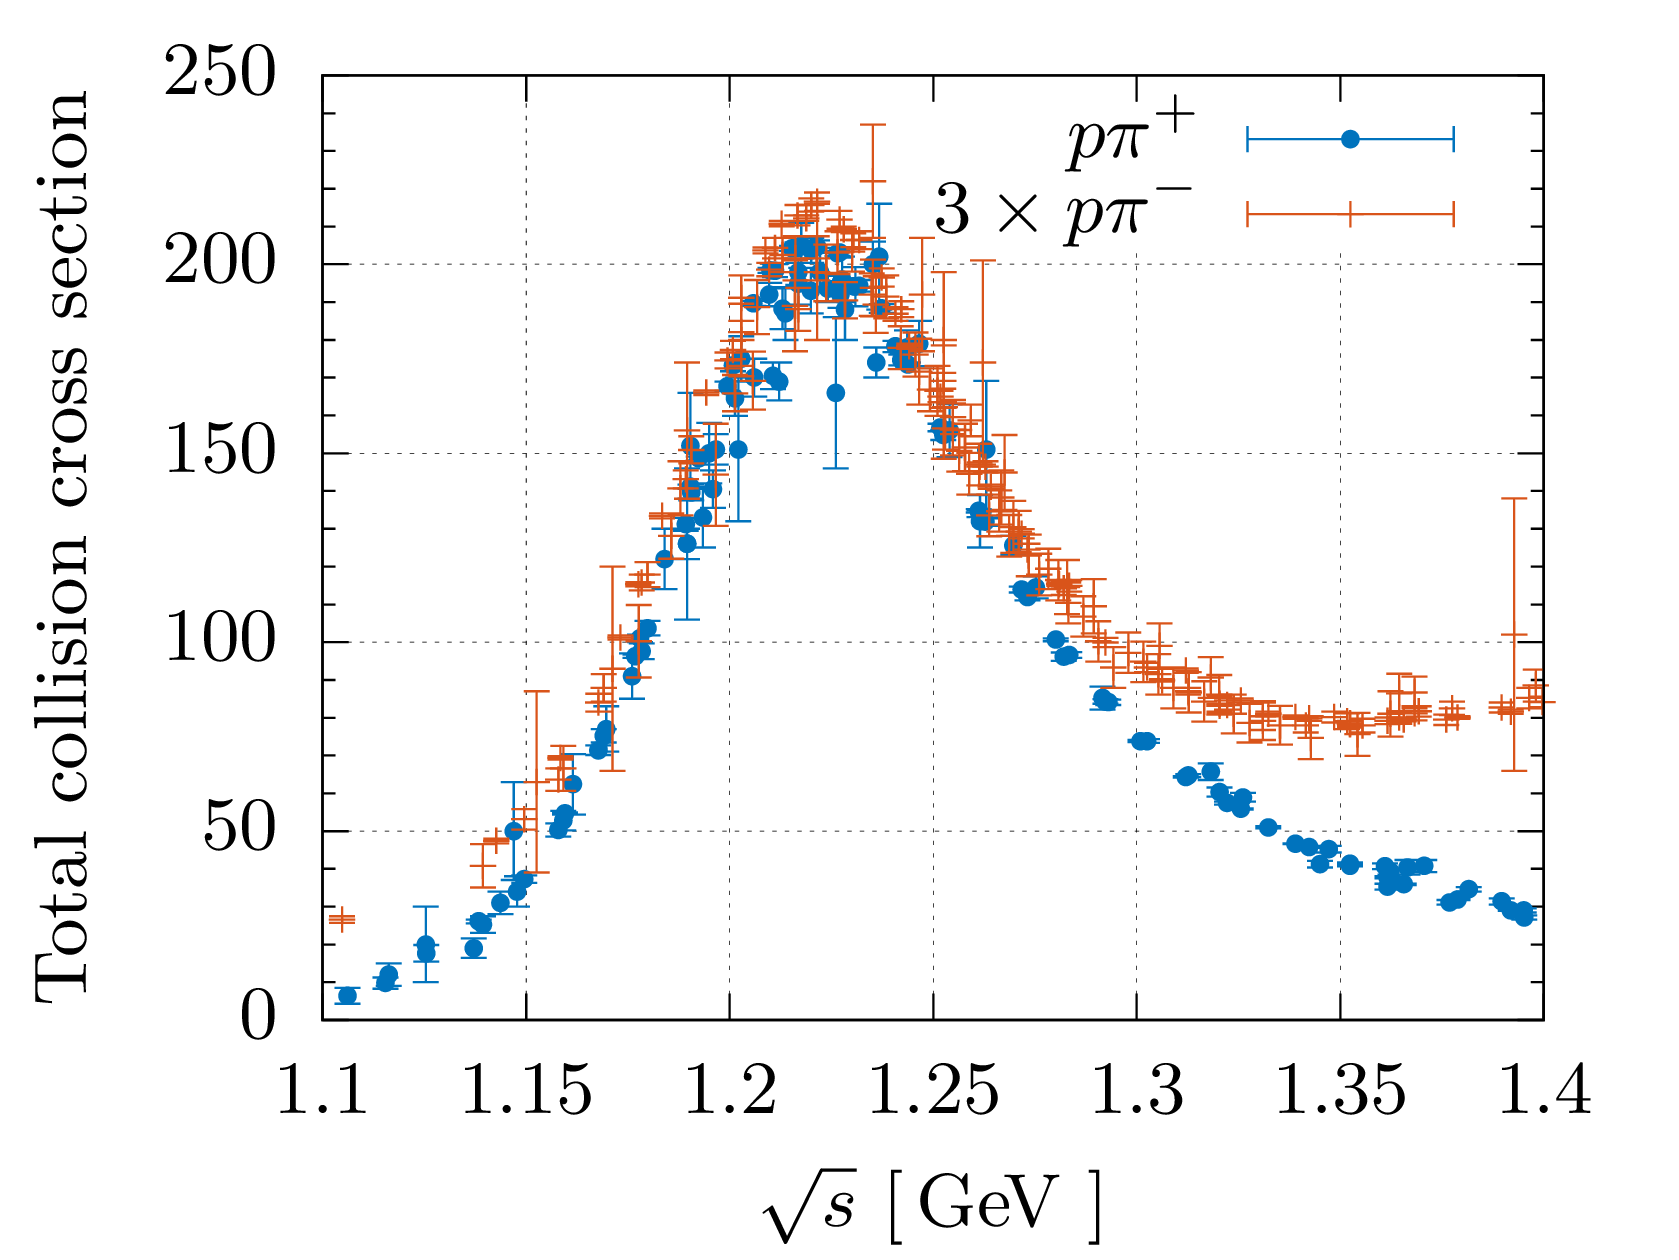
\includegraphics[scale=1.]{misc/pipp_xsec.png}
    \caption{Production rate of $\decay{\proton\pip}{\PDelta(1232)^{++}}$ and $\decay{\proton\pim}{\PDelta(1232)^0}$ with data taken from the Particle Data Group~\cite{ppiTotalSigma}. (Data files are courtesy of the COMPAS Group, IHEP, Protvino, Russia). Isospin conservation predicts an exact ratio of $3$ which is in good agreement with the measurements shown above (note the scaling of the $\proton\pim$ data).}
    \label{fig:ppiTotalSigma}
\end{figure}

An interesting case of isospin violation in strong decays is the decay $\decay{\Peta}{3 \pion}$. This strong decay of a $I^G \left( J^{PC} \right) = 0^+ \left( 0^{-+} \right)$ state into $1^- \left( 0^{-(+)} \right)$ states is forbidden by $G$-parity.
Since $G$-parity is a combination of isospin and $C$-parity and the latter is conserved, this decay indeed violates isospin symmetry.
Interestingly, $\decay{\Peta}{2 \pion}$ decays are forbidden by $C$-parity which makes the $3 \pion$ decays, albeit (approximately) forbidden, the dominant decay modes\footnote{This also explains the exceptionally narrow width of $\Peta$.}~\cite{etaDecays,etaTopippim,etaTopizpiz}
\begin{align*}
    \BR\left(\decay{\Peta}{\pip \pim \piz}\right) &= 22.6 \pm 0.5\,\% \,,\\
    \BR\left(\decay{\Peta}{\piz \piz \piz}\right) &= 34.0 \pm 0.8\,\% \,,\\
    \BR\left(\decay{\Peta}{\pip \pim}\right) &< 1.3 \times 10^{-5} \quad (\text{CL} = 90\%) \,,\\
    \BR\left(\decay{\Peta}{\piz \piz}\right) &< 3.5 \times 10^{-4} \quad (\text{CL} = 90\%) \,,
\end{align*}
and the branching fractions similar to the (isospin violating) electro-magnetic decay $\decay{\Peta}{\gamma\gamma}$~\cite{etaDecays}
\begin{equation*}
    \BR\left(\decay{\Peta}{\gamma\gamma}\right) = 38.5 \pm 0.5\,\% \,.
\end{equation*}
These measurements shine light onto the quantitative power of the isospin argument by showing, that strong, isospin forbidden decays are on the same level as QED transitions ($\mathcal{O}(\alpha^2)$ in this case).
In general, isospin breaking effects can be large in electro-weak decays but are suppressed when strong decays can contribute.
Furthermore, the suppression of isospin violation is considered largely independent of the momentum transfer ($Q$-value), \ie{}, isospin mixes two mass eigenstates, for example
$$\decay{\Lb}{\jpsi \left( \cos(\theta) \Lz + \sin(\theta) \Sigma^0 \right)},$$ 
where the mixing angle $\theta$ is largely independent of the momentum transfer~\cite{privcomGinoIsidori} and thus allows inferring the isospin suppression between decays with different $Q$-values.

\section{\texorpdfstring{\decay{\Sz}{\Lz\Pgamma}}{Σ → Λγ} Background}
\Lz and \Sigmares baryons are part of the baryon octet.
The former is an isospin singlet and the latter three resonances \Sm, \Sz, and \Sp form an isospin triplet.
The quantum numbers of the \Lz and the \Sz baryons are identical, including the common valence quarks (\uquark \dquark \squark), except for the isospin which separates the former as a singlet and the latter as part of the triplet.
The \Sz baryon can thus decay fast without quark transitions into the singlet state \Lz via emission of a soft photon.
Transitions between the \Sz and \Lz via strong interaction are forbidden due to the small isospin splitting, $m(\Sz) - m(\Lz) = 76.959(23)\mevcc$~\cite{pdg}, which is lighter than any meson mass.
Other decay channels besides \decay{\Sz}{\Lz\Pgamma} are $\BR(\decay{\Sz}{\Lz\Pgamma\Pgamma})<3\,\%$ (experimentally measured at a 90\,\% CL) and $\BR(\decay{\Sz}{\Lz\ep\en})= \num{5e-3}$ (theoretical \QED calculation)~\cite{SzToLzgg,SzToLzee}.

Due to the small isospin splitting, the photon of the radiative transition will almost always escape undetected at \lhcb and is therefore not included in the reconstruction step of the present analysis which makes the \Sz resonance a partially reconstructed background in most analyses with intermediate \Lz baryons.

\subsection{Limitations of \texorpdfstring{na\"ive \grpsutw{}}{naive SU(2)} Arguments}
Since both, \Lz and \Sz share the same valence quarks, the decision which of both actually hadronizes in decays is imposed by \QCD.
The production of \Lz and \Sz baryons in \QCD was studied at lepton colliders, \eg{}, by the \gls{besiii} collaboration in \jpsi and \psitwos decays \cite{LzSzProd}.
The results of Ref.~\cite{LzSzProd} are summarized in Tab.~\ref{tab:besiiiJpsiToLzLz}.

\begin{table}[htbp]
    \centering
    \caption{Results for branching fractions \BR of \Lz and \Sz production in charmonia decays taken from Ref.~\cite{LzSzProd}. Statistical and systematic uncertainties are added in quadrature. Additionally, we calculate the ratio of \Sz and \Lz branching fractions, based on the published results of Ref.~\cite{LzSzProd} and assign uncertainties obtained from linear error propagation while ignoring correlations.}
    \label{tab:besiiiJpsiToLzLz}
    \begin{tabular}{l%
                    S[separate-uncertainty=true,table-format=2.2(3)]%
                    c}
        \toprule
        Channel & {\BR~($\times 10^{-4}$)} & {Ratio} \\
        \midrule
        \decay{\jpsi}{\Lz\Lbar} & 19.43 \pm 0.33 & \multirow{2}{*}{\num{0.599 \pm 0.016}} \\
        \decay{\jpsi}{\Sz\Szbar} & 11.64 \pm 0.23 \\
        \decay{\psitwos}{\Lz\Lbar} & 3.97 \pm 0.12 & \multirow{2}{*}{\num{0.615 \pm 0.033}} \\
        \decay{\psitwos}{\Sz\Szbar} & 2.44 \pm 0.11 \\
        \bottomrule
    \end{tabular}
\end{table}

In the case of \Lz and \Sz production from charmonia resonances, hadrons are not only produced via QCD (OZI suppressed decays), but also via QED, \eg{}, \decay{\jpsi}{\decay{\gamma}{\Lz\Lbar}}.
Assuming isospin conservation for QCD, only the latter process gives rise to isospin breaking decays such as \decay{\jpsi}{\Lz \Szbar} which is a transition from an isospin singlet state $\ket{I=0, I_3=0}$ into $\ket{I=1,I_3=0}$.
Even though QED breaks isospin conservation, the single photon allows only one quark anti-quark pair to form a $I=0$ or $I=1$ state.
All other pairs still obey QCD and are thus isospin singlets, \ie{}, only final states of at most $\Delta I=1$ are possible.
The Clebsch-Gordan (CG) coefficients for a \Sz \Szbar pair are
$$\underbrace{\ket{1, 0}}_{\Sz} \otimes \underbrace{\ket{1, 0}}_{\Szbar} = \left\{ \frac{1}{3} \, \ket{0,0},\,\frac{2}{3} \, \ket{2, 0} \right\}.$$
Thus, even in the case of isospin violating $\Delta I=1$ processes, \Lz \Lbar and \Sz \Szbar pairs can only form a $I=0$ state.
Consequently, the branching ratio of \Lz \Lbar and \Sz \Szbar pairs should be governed by the corresponding CG coefficients, and thus be $1$ : $\sfrac{1}{3}$.
Experimentally, a ratio of $60\,\%$ is measured, thus pointing towards an additional isospin breaking contribution, such as final state interactions and possible corrections of a full \grpsuthree{} consideration.
%From a pure isospin consideration, a na\"ive expectation arises from Clebsch-Gordan (CG) coefficients and predicts a factor of $\sfrac{1}{3}$,
%$$\ket{1,0} \otimes \ket{1,0} = \left\{ \frac{1}{3} \, \ket{0,0},\,\frac{2}{3} \, \ket{2, 0} \right\},$$
%where $\ket{I, I_3}$ is an isospin configuration with magnitude $I$ and quantized projection $I_3$.
%Experimentally, however, a ratio of $60\,\%$ is measured, thus hinting towards an enhancement of \Sz resonances w.r.t.\ \Lz beyond angular momentum coupling effects.

When created in (OZI suppressed) strong decays, the initial isospin state of the \uquark-, \dquark- and \squark-quarks is well known due to the isospin conservation of \QCD, whereas the situation is more complicated in weak decays, since isospin conservation is not guaranteed anymore and thus the initial isospin state of the quarks is typically unknown.
\decay{\kaon}{\pion\pion} decays have a long history of revealing counter intuitive selection rules between different isospin states, \ie{}, the amplitudes of \decay{\KS}{\piz\piz}, \decay{\KS}{\pip\pim} and \decay{\Kp}{\pip\piz} can be used to unfold amplitudes corresponding to isospin states $I=0$ and $I=2$.\footnote{The $I=1$ final state is unreachable for pairs of pions due to their bosonic nature, \ie{}, bosons are described by symmetric wave functions, whereas combinations of odd angular momentum $L$ or odd isospin $I$ quantum numbers are antisymmetric. Hence $L$ and $I$ must either be both odd or both even. For kaon decays, $L=0$ and therefore $I$ can have only even values.}
Experimentally, the ratio of the amplitudes for $I=0$ and $I=2$ is measured to be larger than expected from the CG coefficients, thus hinting towards a suppression of large isospins beyond a na\"ive angular momentum coupling description.
In this particular case, this deviation is known as the so-called $\Delta I=\sfrac{1}{2}$ rule for kaons and is well described in theory, for example in the framework of chiral perturbation theory~\cite{DeltaIRule}.

%\subsection{From Emails with Sheldon}
%Gino Isidori / Jon Rosner: However, isospin is broken also in strong interactions by the quark masses. It is a small effect, but non zero (indeed we have \decay{\Peta}{\pion \pion \pion}, \Prho-\Pomega mixing...). So, I expect  \decay{\Lb}{\jpsi\Sz} to occur at a significantly lower rate than \decay{\Lb}{\jpsi \Lz}, but to be there. Actually the $m(\uquark)-m(\dquark)$ mass difference corresponds indeed to a $\Delta I = 1$ operator.
%
%Zoltan Ligeti: I do not think about isospin violation in terms of these Feynman diagrams.  The ($\bquark \cquarkbar \cquark \squarkbar$) part of the weak Hamiltonian (from integrating out the \W), pictured in the diagram you sent me, will generate both decays, but the \Sz final state should be substantially suppressed compared to the \Lz final state, as the former is isospin violating. I think it is definitely worth measuring!  We have very little data on how significant a suppression corresponds to isospin violation in these type of decays, it can teach us about QCD, SCET, factorization, etc.
%
%Roland: \decay{\Peta}{\pion \pion \pion}: hier schlaegt wieder mal die G-Paritaet zu: \Peta hat +, 3 Pionen haben -. Und G-Paritaet beruht auf C-Paritaet und Isospin. Da wir annehmen, dass C erhalten ist, ist der Isospin verletzt. Das ist in der Tat ein interessantes Beispiel, da vermutlich die elmgn. WW. (die Isospin verletzt) nicht ausreicht. Meines Wissens spielt dabei eine Rolle, dass die pis und das \Peta relativ leicht sind, sodass die kleine MAssendifferenz \dquark-\uquark ein messbaren $\Delta I$ Uebergang bewirken kann. Isospinverletzung gibt es (im Prinzip in grossem Stil) in der schwachen WW und der elmgn. WW.  Beide sind aber viel schwaecher als die starke WW, weshalb Isospinverletzung meist ein kleiner Effekt ist, wenn die starke WW auch beitragen kann. Darueberhinaus verletzen die Yukawa-Kopplungen des Higgs auch den Isospin, d.h. u und d haben verschiedene Massen.
%Das spielt immer dann eine Rolle, wenn die Q-Werte klein sind.

\subsection{Background Contamination by \texorpdfstring{\decay{\Sz}{\Lz\Pgamma}}{Σ → Λγ} at \lhcb}
Since the soft photon in \decay{\Sz}{\Lz\Pgamma} cannot be reconstructed at \lhcb, most analysis with intermediate \Lz resonances will be contaminated with the partially reconstructed background events of \Sz decays which are irreducible.

For example, this is the case in the charmless two-body decay \decay{\Bu}{\proton\Lbar}, analyzed at \lhcb~\cite{BuTopLzb}.
Penguin contributions with a \decay{\bquarkbar}{\squarkbar} loop are expected to dominate, but tree-level and annihilation diagrams also contribute.
Electro-weak penguins and tree diagrams create a \uquark\uquarkbar or \dquark\dquarkbar pair that couples with the spectator quark either into an isospin $I=\sfrac{1}{2}$ or $I=\sfrac{3}{2}$ state, corresponding to $\Delta I = 0$ and $\Delta I = 1$, respectively.
The other \quark\quarkbar pair is created from the QCD vacuum and thus does not change the total isospin.
In case of the annihilation diagram and gluon penguins, two \quark\quarkbar pairs are created form the QCD vacuum and only $\Delta I=0$ is possible.

%Here, the \dquark \dquarkbar vacuum pair is an isospin singlet, whereas the quarks from the quark transition \decay{\bquark}{\uquark \squark \uquarkbar} (tree or penguin diagram) and the spectator quark can form an isospin doublet and quadruplet state,
%\begin{equation}
%    \label{eq:BuTopLzbQuarks}
%    \underbrace{\ket{0, 0}}_{\text{vacuum}} \otimes \underbrace{\ket{\frac{1}{2}, +\frac{1}{2}} \otimes \ket{\frac{1}{2}, -\frac{1}{2}}}_{\bquarkbar \, \to \, \uquarkbar \, \squarkbar \uquark} \otimes \underbrace{\ket{\frac{1}{2}, +\frac{1}{2}}}_{\text{spectator}} = \left\{ \frac{2}{3} \, \ket{\frac{1}{2}, \frac{1}{2}},\, \frac{1}{3} \, \ket{\frac{3}{2}, \frac{1}{2}} \right\}.
%\end{equation}
The quark states can hadronize as either \proton\Lbar or \proton\Szbar, \ie{},
\begin{align*}
    \proton\Lbar &: \quad \ket{\frac{1}{2}, \frac{1}{2}} \otimes \ket{0, 0} = \ket{\frac{1}{2}, \frac{1}{2}} \,,\\
    \proton\Szbar &: \quad \ket{\frac{1}{2}, \frac{1}{2}} \otimes \ket{1, 0} = \left\{ \frac{1}{3} \, \ket{\frac{1}{2}, \frac{1}{2}},\, \frac{2}{3} \ket{\frac{3}{2}, \frac{1}{2}} \right\} \,.
\end{align*}
Inferring a suppression of $\Delta I=1$ from the $\Delta I=\sfrac{1}{2}$ selection rule for kaons, \Sz resonances would be suppressed by a factor of $\sfrac{1}{3}$. Vice-versa, if $\Delta I = 0$ would be suppressed, then electro-weak penguins and tree diagrams would induce an increase of \Sz hadronization.
The fit to recorded \decay{\Bu}{\proton\Lbar} events at \lhcb prefers the former option by finding $N(\decay{\Bu}{\proton\Szbar})$ being compatible with zero but $N(\decay{\Bu}{\proton\Lbar}) = 13.0^{+5.1}_{-4.3}$~\cite{BuTopLzb}.
We note, that the amount of available statistics in this channel is similar to \decay{\Lb}{\Dz\Lz} where we expect the very same suppression factor.
(Even without relying on \enquote{mysterious $\Delta I$ rule[s]}, \cf Ref.~\cite{DeltaIRule}.)

In Tab.~\ref{tab:SzInLbDecays} we show a selection of \Lb decays with an intermediate \Lz baryon together with the corresponding \Lz-\Sz asymmetry
\begin{equation}
    \label{eq:theory_lzszasym}
    a(\Lz : \Sz) := \frac{f(\Lz) - f(\Sz)}{f(\Lz) + f(\Sz)} \,,
\end{equation}
where $f(\Lz)$ and $f(\Sz)$ refer to the amounts of \Lz and \Sz, respectively.
An asymmetry of $-1$, $0$, $+1$ thus corresponds to a pure \Sz, balanced \Lz and \Sz, and pure \Lz decay, respectively.

For some of the decays listed in Tab.~\ref{tab:SzInLbDecays} \W-exchange diagrams are also possible (\eg{}, Ref.~\cite{wexchange}) which are often considered suppressed in the literature.
We note, that a strong suppression is only given for mesons due to the required spin alignment of the quark and anti-quark pair, but that this is not necessarily the case for baryons.

The decays $\decay{\Lb}{\Lz\Ph\Ph'}$, \decay{\Lb}{\Lz\Pphi} and \decay{\Lb}{\jpsi\Lz} were analyzed at \lhcb~\cite{LbToLzhh,LbToLzphi,LbToJpsiLz}, whereas the other decays are subject of the present analysis.
The ranges for the values of the \Lz-\Sz asymmetry arises from the yet unknown $\Delta I$ selection rules we mentioned above.
For example, the \uquark-quark produced via \W-exchange in the \decay{\Lb}{\Lz\Pphi} decay can either end within a $\ket{0, 0}$ or a $\ket{1, 0}$ state together with the spectator, corresponding to a \Lz-\Sz asymmetry of either $1$ or $-1$, respectively.
In the case of tree and penguin decays of the \Lb baryon, we can further constrain the possible combinations by observing, that the spectator diquark (\uquark \dquark) is an isospin singlet state $\ket{0, 0}$ which is, since not involved in the decay in leading order, conserved.
In decays via \W-exchange, this initial singlet state is broken, though, and the spectator quark can contribute in the subsequent isospin coupling.
\begin{table}[htbp]
    \centering
    \caption{Selection of \Lb decays with an intermediate \Lz baryon, primary quark transitions, and \Lz-\Sz asymmetry $a(\Lz:\Sz)$ as defined in Eq.~\eqref{eq:theory_lzszasym}. For decays via \W-exchange the spectator quark has to be included into the isospin coupling (flavor is shown in parentheses).}
    \label{tab:SzInLbDecays}
    \begin{tabular}{lllc}
        \toprule
        Channel & Quark transition && \Lz-\Sz asymmetry \\
        \midrule
        \decay{\Lb}{\Lz\pip\pim} & \decay{\bquark}{\uquark \squark \uquarkbar} & (tree \& penguin) & $\sfrac{1}{9} \ldots \sfrac{1}{3}$ \\
        & \decay{\bquark}{\squark \dquark \dquarkbar} & (penguin) & $\sfrac{1}{9} \ldots \sfrac{1}{3}$ \\
        & \decay{\bquark \uquark (\dquark)}{\uquark \squark (\dquark)} & (exchange) & $\sfrac{1}{9} \ldots \sfrac{1}{3}$ \\
        \midrule
        \decay{\Lb}{\Lz\Kp\pim} & \decay{\bquark}{\uquark \dquark \uquarkbar} & (tree \& penguin) & $-\sfrac{1}{6} \ldots \sfrac{1}{3}$ \\
        & \decay{\bquark}{\dquark \squark \squarkbar} & (penguin) & $\sfrac{1}{3}$ \\
        & \decay{\bquark \uquark (\dquark)}{\uquark \dquark (\dquark)} & (exchange) & $-\sfrac{1}{6} \ldots \sfrac{1}{3}$ \\
        \midrule
        \decay{\Lb}{\Lz\Kp\Km} & \decay{\bquark}{\squark \uquark \uquarkbar} & (tree \& penguin) & $0 \ldots \sfrac{1}{2}$ \\
        & \decay{\bquark}{\squark \squark \squarkbar} & (penguin) & $\sfrac{1}{2}$ \\
        & \decay{\bquark \uquark (\dquark)}{\uquark \squark (\dquark)} & (exchange) & $0 \ldots \sfrac{1}{2}$\\
        \midrule
        \decay{\Lb}{\Lz\Pphi} & \decay{\bquark}{\squark \squark \squarkbar} & (penguin) & $1$ \\
        & \decay{\bquark \uquark (\dquark)}{\uquark \squark (\dquark)} & (exchange) & $-1 \ldots 1$ \\
        \midrule
        \decay{\Lb}{\jpsi\Lz} & \decay{\bquark}{\cquark \cquarkbar \squark} & (tree \& penguin) & $1$ \\
        & \decay{\bquark \uquark (\dquark)}{\uquark \squark (\dquark)} & (exchange) & $-1 \ldots 1$ \\
        \midrule
        \decay{\Lb}{\Dz\Lz} & \decay{\bquark}{\cquark \uquarkbar \squark} & (tree) & $\sfrac{1}{2}$ \\
        & \decay{\bquark \uquark (\dquark)}{\cquark \squark (\dquark)} & (exchange) & $\sfrac{1}{2}$ \\
        \midrule
        \decay{\Lb}{\Dzb\Lz} & \decay{\bquark}{\uquark \squark \cquarkbar} & (tree) & $\sfrac{1}{2}$ \\
        \midrule
        \decay{\Xibz}{\Dz\Lz} & \decay{\bquark}{\cquark \dquark \uquarkbar} & (tree) & $-1 \ldots \sfrac{1}{2}$ \\
        & \decay{\bquark \uquark (\squark)}{\cquark \dquark (\squark)} & (exchange) & $\sfrac{1}{2}$ \\
        \midrule
        \decay{\Xibz}{\Dzb\Lz} & \decay{\bquark}{\uquark \dquark \cquarkbar} & (tree) & $-1 \ldots \sfrac{1}{2}$ \\
        \bottomrule
    \end{tabular}
\end{table}

Most interesting for the present analysis is the ratio of the absolute amount of reconstructed decays with intermediate \Lz and \Sz in order to estimate the background contamination of \decay{\Lb}{\Dz\Sz} in \decay{\Lb}{\Dz\Lz}.
Unfortunately, there are a couple of caveats with na\"ively interpreting the yields of the fitted modes.
For example in the analysis of $\decay{\Lb}{\Lz\Ph\Ph'}$ decays, the authors could only account for partially reconstructed background components with a missing soft photon in general, due to the lack of experimental data of further \Lb background candidates~\cite{LbToLzhh}.
Contributions of \decay{\Sz}{\Lz\Pgamma} are, however, most physically motivated, but only one reasonable instance.
Unfortunately, the partially reconstructed background \decay{\Sz}{\Lz\Pgamma} peak in roughly the same place as the cross-feed contribution, which is quite well understood, but as the corresponding signal yields are small, this results in a reasonable uncertainty on which contributions are which.
Additionally, the same problem occurs in the \decay{\Lb}{\Lc\Ph} control mode where the \Lc can either decay into \Lz \pip or \Sz \pip.
Both of these amplitudes are measured by the \gls{besiii} collaboration and found to be significantly greater than zero~\cite{LcBR} and thus pollute the interpretation of the fitted yields as the true charmless decays, without \Lc component.
Luckily for the present analysis, this effect is most pronounced in the \Lz\pip\pim final state (\cf{}~Chap.~\ref{chap:bkgs}).
The branching fractions for corresponding modes with kaons are considerably more suppressed.

\subsection{Summary}
Isospin (non-)conservation is helpful for deciding whether or not a decay is suppressed.
Finding exact branching ratios, though, can be error prone as we saw in the case of \Lz\Lbar vs.\ \Sz\Szbar production or due to yet unknown $\Delta I$ selection rules.
However, in the case of \decay{\Lb}{\Dz\Lz} the situation is much easier and we do not expect large corrections neither to the tree, nor to the \W-exchange diagram. 

Regarding the available statistics, we will not be able to constrain or extract the relative branching ratio but we find it noteworthy to mention, that the \Sz modes are of great interest for future experiments for at least two reasons:
First, for the same reasons \CP violation is expected in \decay{\Lb}{\PD\Lz}, it is also expected for \decay{\Lb}{\PD\Sz} with different strong phases.
Secondly, \grpsuthree{} considerations yield relations among the amplitudes of \decay{\Lb}{\Dz\PX} and \decay{\Xibz}{\Dz\PX} decays~\cite{privyuval}:
\begin{align*}
    1 - \sqrt{3} \frac{\mathcal{A}(\decay{\Lb}{\Dz\Lz})}{\mathcal{A}(\decay{\Lb}{\Dz\Sz})} + \sqrt{2} \frac{\mathcal{A}(\decay{\Xibz}{\Dz\Xiz})}{\mathcal{A}(\decay{\Lb}{\Dz\Sz})} &= 0 \,, \\
    1 + \sqrt{3} \frac{\mathcal{A}(\decay{\Lb}{\Dz\Lz})}{\mathcal{A}(\decay{\Lb}{\Dz\Sz})} - 2 \frac{\lambda_s}{\lambda_d} \frac{\mathcal{A}(\decay{\Xibz}{\Dz\Sz})}{\mathcal{A}(\decay{\Lb}{\Dz\Sz})} &= 0 \,, \\
    1 - 2 \frac{\lambda_d}{\lambda_s} \frac{\mathcal{A}(\decay{\Lb}{\Dz\Sz})}{\mathcal{A}(\decay{\Xibz}{\Dz\Sz})} + \sqrt{3} \frac{\mathcal{A}(\decay{\Xibz}{\Dz\Lz})}{\mathcal{A}(\decay{\Xibz}{\Dz\Sz})} &= 0 \,, \\
    1 - \sqrt{3} \frac{\mathcal{A}(\decay{\Lb}{\Dz\Lz})}{\mathcal{A}(\decay{\Lb}{\Dz\Sz})} + \sqrt{2} \frac{\lambda_s}{\lambda_d} \frac{\mathcal{A}(\decay{\Lb}{\Dz\neutron})}{\mathcal{A}(\decay{\Lb}{\Dz\Sz})} &= 0 \,,
\end{align*}
with
\begin{align*}
    \lambda_d &:= \Vuds\Vcb \,, \\
    \lambda_s &:= \Vuss\Vcb \,.
\end{align*}
These should be tested and used to constrain decays that are unavailable for current experiments such as \decay{\Lb}{\Dz\neutron}.

\section{\texorpdfstring{\CP Violation in \bquark-Baryon Decays}{CP Violation in b-Baryon Decays}}
\label{sec:lbcpv}
\CP violation is an interference effect and originates from the complex phases of the \gls{ckm} matrix.
In order to get a measurable physical quantity in amplitudes the given observable has to come from the superposition of two (or more) decay modes that contribute a \CP even and a \CP odd term (\gls{ckm} phases are \CP odd) such that the interference term does not cancel in the magnitude.
In general, such decay modes are categorized into three classes, direct \CP violation, \CP violation in mixing, and \CP violation in interference of mixing and decays (\cf{} any good text book about flavor physics for more details).
Mesons offer a rich laboratory for measuring \CP violation among all three classes, \eg{}, Refs.~\cite{bsmixing,BsTohh_timecpv}.
In baryonic systems, and in particular in decays of \bquark-baryons such as the \Lb or \Xibz baryon, there can be no mixing due to conservation of baryon number and therefore no indirect \CP violation.
Studies of direct \CP violations are often limited to measuring asymmetries, since the \CP even phases have to be taken from theory which makes the result model dependent and typically come with large uncertainties~\cite{LbCPVAsym1,LbCPVAsym2}.
Lately, two methods have been proposed to overcome this issue~\cite{CPVbeautiful,brLbToDzLz_pred}.
They reinterpret methods original proposed by Atwood, Dunietz and Soni~\cite{ads1,ads2}, referred to as \gls{ads}, and a method first proposed by Gronau, London and Wyler~\cite{glw1,glw2}, referred to as \gls{glw}, that are already successfully carried out in decays of mesons~\cite{BdToDzKstar}, now for decays of baryons.
As proposed, these methods allow a clean extraction of the \gls{ckm} phase $\gamma$ in a model independent way\footnote{In particular the proposed modes do not suffer from penguin pollution.} and at the same time neither require tagging nor time-dependence.
In particular, in the \gls{ads} method $\gamma$ can be extracted by the study of the six decays \decay{\Lb}{\Dz\Lz}, \decay{\Lb}{\Dzb\Lz}, $\decay{\Lb}{\PD_{\CP}\Lz}$, and the respective \Lbbar modes, where
\begin{equation*}
    \PD_{\CP} \equiv
    \begin{dcases}
        \frac{\ket{\Dz} + \ket{\Dzb}}{\sqrt{2}} & \text{if \CP-even modes are considered,} \\
        \frac{\ket{\Dz} - \ket{\Dzb}}{\sqrt{2}} & \text{else.}
    \end{dcases}
\end{equation*}
Key to the present analysis is the idea, to enhance the \CP violating contribution by reconstructing $\decay{\Lb}{[\Kp\pim]_{\PD}\Lz}$ which compensates the suppression of \decay{\Lb}{\Dzb\Lz} by favoring the Cabibbo (doubly) suppressed \decay{\Dz}{\Kp\pim} mode in the \decay{\Lb}{\Dz\Lz} decay (\cf{}~Fig.~\ref{fig:decaysLbToDzLz}).
\begin{figure}
    \centering
    \begin{subfigure}{.49\textwidth}
        \centering
        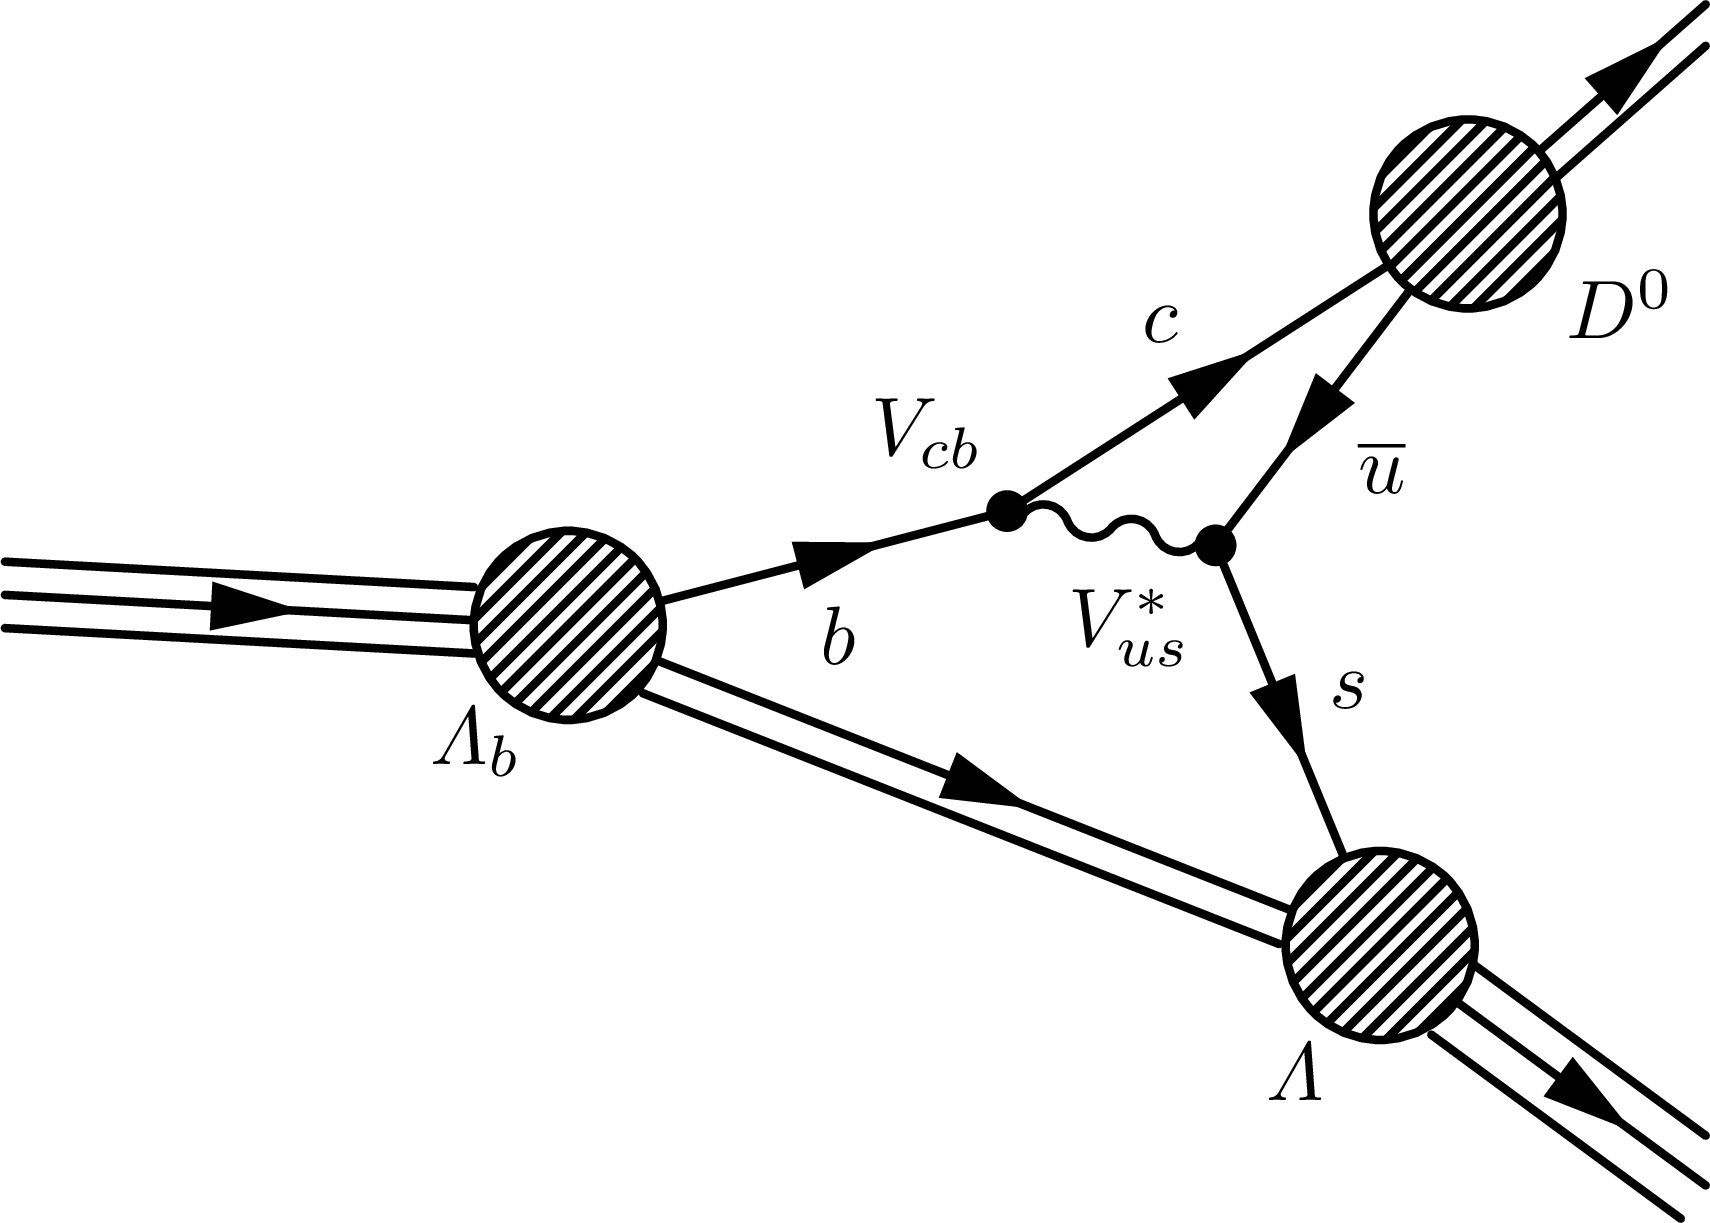
\includegraphics[scale=.1]{misc/decayLb2DzLz.png}
        \caption{\decay{\Lb}{\Dz\Lz}}
    \end{subfigure}
    \begin{subfigure}{.49\textwidth}
        \centering
        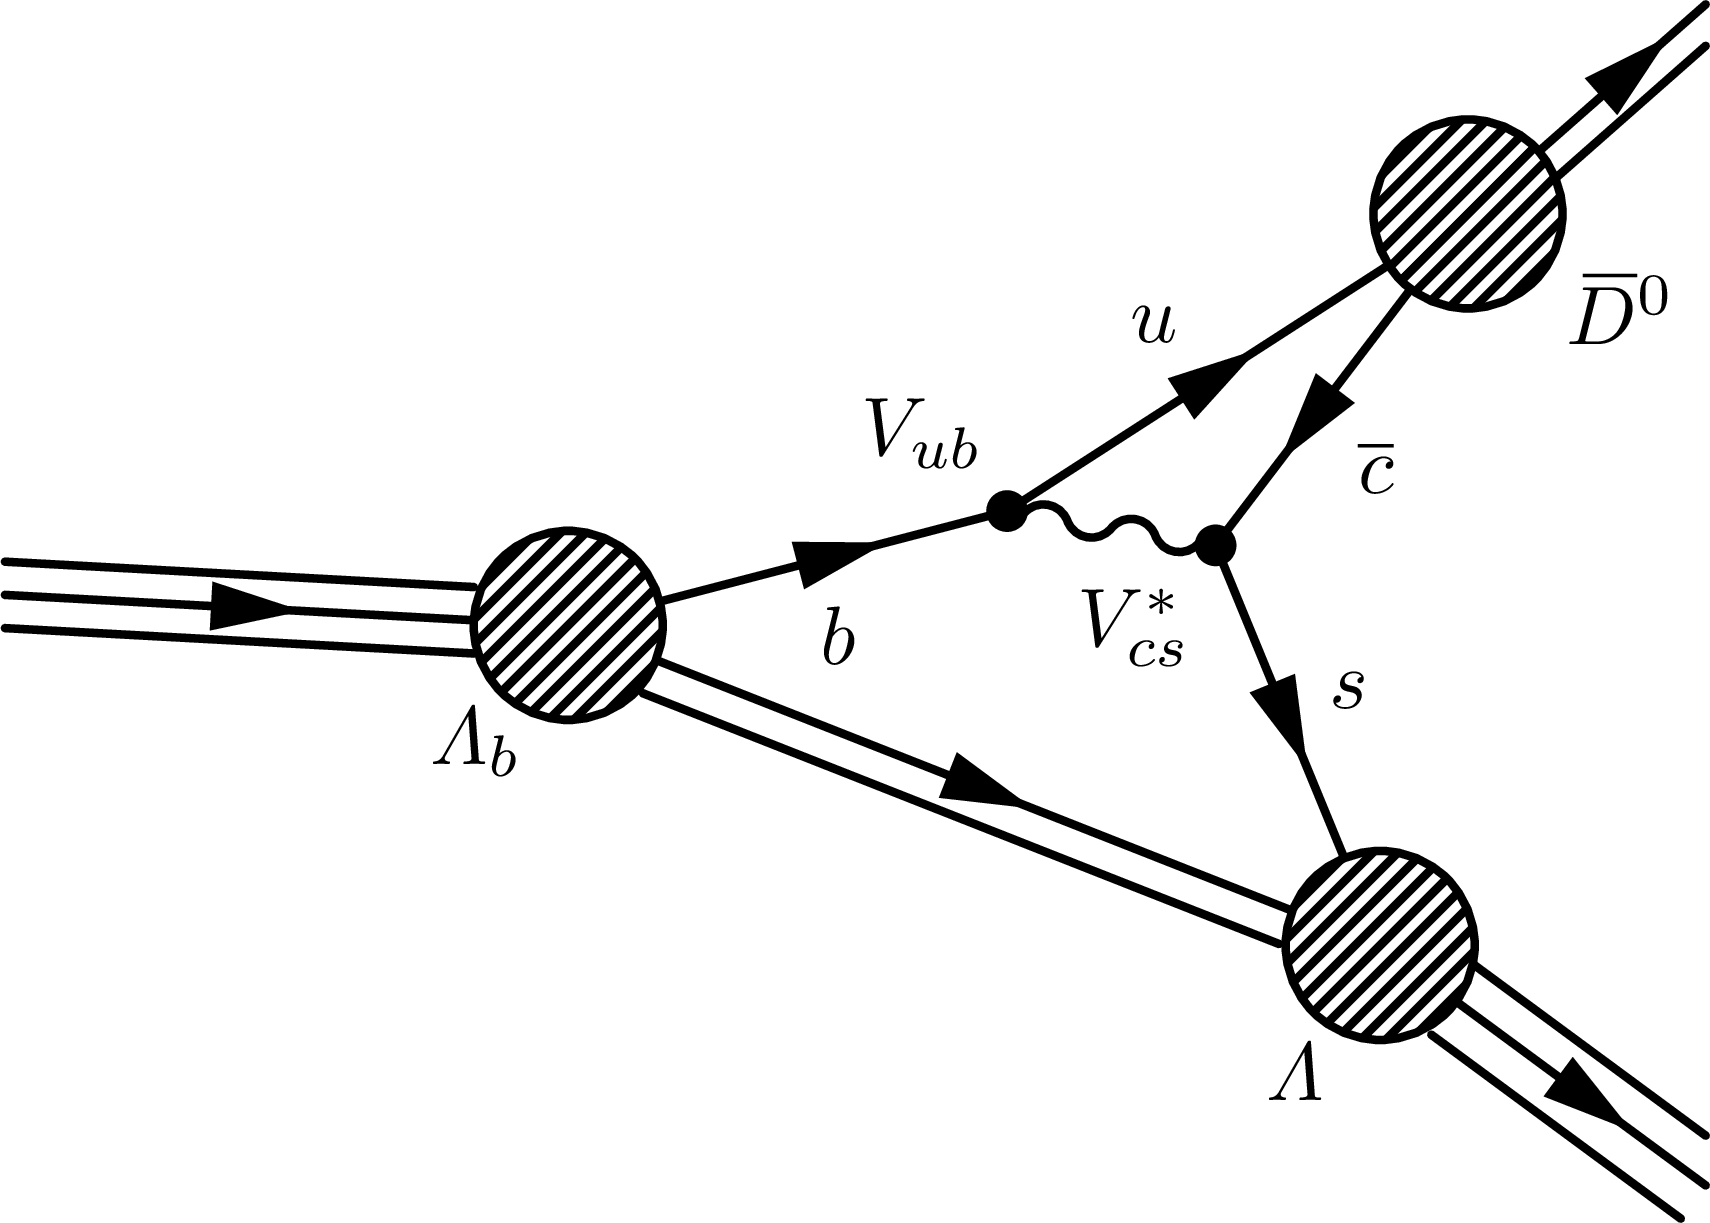
\includegraphics[scale=.1]{misc/decayLb2DzbLz.png}
        \caption{\decay{\Lb}{\Dzb\Lz}}
    \end{subfigure}
    \caption{Feynman diagrams of the decays \decay{\Lb}{\Dz\Lz} and \decay{\Lb}{\Dzb\Lz}. The latter decay is strongly suppressed w.r.t.\ to the former due to the \decay{\bquark}{\uquark} transition. The suppression can be reduced by reconstructing \decay{\PD}{\Kp\pim} which is Cabibbo doubly suppressed for the former but Cabibbo favored for the latter.}
    \label{fig:decaysLbToDzLz}
\end{figure}
Further, the statistics of the studies can be enriched by also including the four-body modes $\decay{\PD}{\Kpm\pimp\pip\pim}$.
Similarly, the same technique is applicable to other two-body decays, such as $\decay{\Xires_\bquark^{0/-}}{\PD\Xires^{0/-}}$ and $\decay{\Omegab}{\PD\Omegares^0}$ but also to the various backgrounds of the present analysis (\cf{}~Chap.~\ref{chap:bkgs}) and also three-body decays such as \decay{\Lb}{\Dz\proton\Km} or \decay{\Lb}{\Lz\pip\pim}~\cite{cpvinLbToLzpipi}. (The latter is also well suited for measurement of $T$ violation with triple products~\cite{tvinLbToLzpipi}.)
We note further that in all these modes, the \CP violation is encoded in the entire decay chain, do not rely on \CP violation in the \PD meson system and thus genuinely leverages the observation of \CP violation in baryon decays. 
The same holds for the cited \gls{glw} method where the \Dz and \Dzb are reconstructed in \CP eigenstates \Kp\Km and \pip\pim.

In contrast to the two-body decay modes, the three-body decay modes have to be studied in Dalitz plots that require a meticulous description of the various background and resonance contributions.
%In particular, the many resonances in \decay{\Lb}{\Dz\proton\Km} studies require thorough analyses~\cite{hviemann}.
On the contrary, two-body decays come with significant smaller sample sizes at \lhcb, due to the lower branching fraction, and reconstruction and trigger inefficiencies of the long living \Lz baryons, but offer a much easier to analyze decay topology.
Since none of the \decay{\Lb}{\PD\Lz} decays have been observed at the time of writing, the main focus of the present analysis is to establish a branching ratio for \decay{\Lb}{\Dz\Lz} by reconstructing \decay{\Dz}{\Km\pip} (and thus neglecting Cabibbo doubly suppressed contributions from \decay{\Lb}{\Dzb\Lz}).
We find the available dataset also sensitive to the decay \decay{\Xibz}{\Dz\Lz} which is on its own a candidate for measuring \CP violation.
We note that a \CP violation study of the \Xibz decay using the \gls{ads} method does not suffer from a contamination of charmless backgrounds\footnote{Due to the absence of \decay{\Xibz}{\Lz\Kp\pim} decays, \cf{}~Sec.~\ref{sec:bkgs_refl}.} as it is the case for \CP violation studies of the corresponding \Lb decay, whereas the expected amount \CP violation is much lower.

\chapter{The LHCb Detector at the LHC}
\label{chap:detector}
%\chapquote{Teamwork is essential. It allows you to blame someone else.}{Finagle's Rule.}
The \lhcb experiment is one of the four major \gls{hep} experiments at the Large Hadron Collider (\lhc) and understands its primary focus in the realm of \bquark- and \cquark-physics.
The  \lhc is a particle accelerator located at the \cern facility.
Its main component is a storage ring with a total length of \SI{26.7}{\kilo\meter} in which protons are collided symmetrically.
At the time of writing the \lhc is the most powerful particle accelerator in the world.\footnote{Although powerful, it will most likely not destroy earth~\cite{lhcdestroyworld1,lhcdestroyworld2}.}
Since the year 2011, the proton beam energy has increased from \SI{3.5}{\tera\electron\volt} to \SI{4}{\tera\electron\volt} in the year 2012 and to \SI{6.5}{\tera\electron\volt} in the year 2015.
The periods of data taking are divided into the so-called \gls{runone} and \gls{runtwo} where the former refers to the years 2011 and 2012 and the latter to the years 2015 until 2018, corresponding to and integrated luminosity of roughly 3\,\invfb and 6\,\invfb, respectively.

Due to the large center-of-mass energy at the \lhc the highly correlated \bquark- and \bquarkbar-hadrons are predominately produced in the same forward or backward cone.
The \lhcb detector is thus designed as a (single arm) forward spectrometer, covering a forward cone from \SI{15}{\mrad} to \SI{300}{\mrad} in the bending plane and \SI{15}{\mrad} to \SI{250}{\mrad} in the non-bending plane.
The detector configuration consists of several tracking stations and calorimeters to reconstruct charged and neutral particles.
An effective particle identification is provided by a large dipole magnet and two Cherenkov radiators.
Different stages of hard- and software triggers reduce the event rate to a frequency at which events can be stored to disks.

In the present analysis we analyze the full available \gls{runtwo} dataset, recorded in the years 2015 until 2018.
Data recorded during the years 2011 and 2012 (\gls{runone}) are not taken into account for several reasons: First, from a technical point of view the experimental setup was frequently changed during \gls{runone}.
This includes changes to the trigger configuration which would require a separate analysis of data recorded during 2011 and the first and second half of 2012.
Secondly, only the second half of 2012 includes an efficient dedicated \Lz trigger, diminishing the total selection efficiency of the previous parts.
Thirdly, even though the \Lb production fraction is larger at small energies, this advantage is overcompensated by far due to the smaller \bbbar cross-section, making \gls{runtwo} significantly more efficient in terms of the overall signal efficiency.
Taking into account the larger data sample in terms of luminosity we conclude that adding \gls{runone} data could not help to significantly improve our results, but would imply disproportionate larger complexity and is therefore disfavored.

\section{Experimental Setup}
In the following we give a short overview about a selection of detector components that are relevant for the present analysis.
More detailed information, illustrations and thorough descriptions of the entire detector can be found in Refs.~\cite{lhcbdet,lhcbPerformance_run1}.
\begin{figure}[htbp]
    \centering
    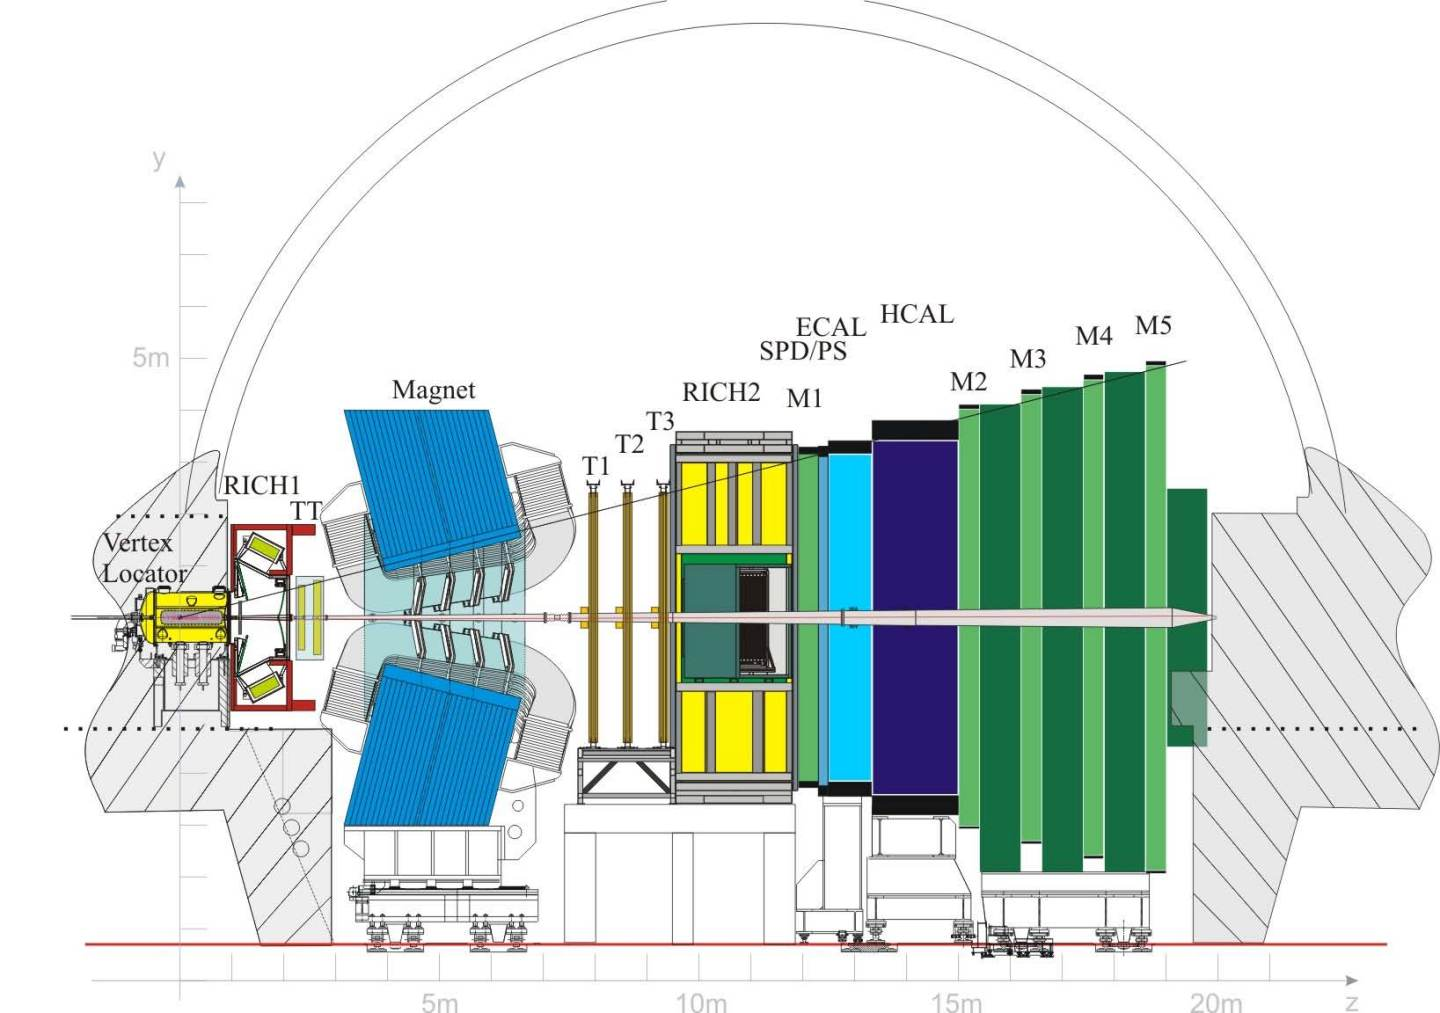
\includegraphics[width=.8\textwidth]{misc/lhcb_detector.png}
    \caption{Schematic view of the \lhcb detector by R.~Lindner (2008).}
\end{figure}

\subsection{Tracking}
\label{sec:detector_tracking}
A vertex locator (\gls{velo}) provides the precise measurements of tracks near of the \proton\proton interaction point.
Besides track reconstruction this information is also useful to distinguish primary vertices (\gls{pv}), \eg{}, from particles originating directly from the interaction point, and secondary vertices from long living \bquark- and \cquark-hadrons.
The \gls{velo} consists of \num{42} silicon modules, each of them equipped with radial and azimuthal strips.
The modules are semicircularly shaped and arranged in pairs such that they surround the beam pipe perpendicularly.
The pitches of the silicon sensors increase linearly from \SI{38}{\micro\meter} at the inner radius ($r=\SI{8.2}{\milli\meter}$) to \SI{102}{\micro\meter} at the outer radius ($r=\SI{42}{\milli\meter}$).
The spatial design of the modules was chosen such that charged particles with a pseudo rapidity $1.6 < \eta < 4.9$ cause at least three hits inside the \gls{velo}.
The total length of the \gls{velo} is not sufficient to cover all end vertices of long living $\PV^0$ particles such as the \Lz baryon or the \KS meson.
If both daughters of a $\PV^0$ two-body decay are reconstructed within the \gls{velo} we refer to the reconstructed tracks as long tracks (\gls{LL}).
Otherwise, if the reconstruction is only based on hits in the tracking stations TT and T1-T3, we refer to them as downstream tracks (\gls{DD}).
For the sake of brevity, we categorize entire decays chains, such as \decay{\Lb}{\Dz\Lz}, also as \gls{LL} (\gls{DD}) if both \Lz daughters are reconstructed as long (downstream) tracks.

Besides the \gls{velo}, four more tracking systems are placed, referred to as the TT, located upstream, and the modules T1, T2 and T3, located downstream of the spectrometer magnet.
The TT and the inner parts of the T1-T3 stations are constructed from p-on-n silicon microstrips detectors with a hit efficiency above 99\,\% and a hit resolution of approximately \SI{50}{\micro\meter}.
%The TT is \SI{150}{\centi\meter} wide and \SI{130}{\centi\meter} high.
The silicon microstrips are arranged in four layers, corresponding to an active area of approximately \SI{8}{\meter\squared}.
The resolution of the T1-T3 stations varies from the innermost towards the outer parts.
Whereas silicon strips are used for the inner parts, the outer parts of the T1-T3 stations are straw-tubes.
The straw-tubes measure the drift time of ionised charges with a total delay below \SI{75}{\nano\second}.

\subsection{Ring Imaging Cherenkov Detectors}
Two Ring Imaging Cherenkov detectors (\gls{rich}), referred to as RICH1 and RICH2, detect Cherenkov light.
Cherenkov radiation is an electromagnetic radiation that gets emitted by charged particles in a dielectric medium if the velocity $v$ of the particles is greater than the (group) velocity $c_m$ of the given medium.
For constant velocities the emitted light cone has a constant opening angle $\phi$,
\begin{equation*}
    \sin \frac{\phi}{2} = \frac{c_m}{v} = \frac{c_0}{nv} \,,
\end{equation*}
and thus directly allows the inference of $v$ if the refractive index $n$ (and the speed of light in vacuum $c_0$) is known.
Inside the \gls{rich} units, Cherenkov cones are mapped to spherical coordinates $(r,\vartheta)$, where $r$ is a function of the opening angle $\phi$ and $\vartheta$ is the azimuthal part of the Cherenkov photons trajectory.
This projection is achieved via spherical mirrors which reflect the photons to Hybrid Photon Detectors where they are detected.
By combining the measurements of the opening angle $\phi$ as a function of $v$ and the deflection in the magnetic field, a hypothesis for the invariant mass can be set and thus allow to identify the particle (\cf{} Sec.~\ref{sec:detector_pid}).
%Although vacuum could be used as a radiator in theory~\cite{vacuumcherenkov}, each \gls{rich} unit is filled with a different gas admixture, corresponding to different refractive indices to lower the Cherenkov thresholds and to allow a diverse momentum resolution.
Each \gls{rich} unit is filled with a different gas admixture, corresponding to different refractive indices to lower the Cherenkov thresholds and to allow a diverse momentum resolution.
Since \gls{runtwo}, RICH1 is filled with $\mathrm{C}_4\mathrm{F}_{10}$, whereas $\mathrm{CF}_4$ is used as the radiator in RICH2, making the units sensitive to the momentum ranges $2$ to $60\,\gevc$ and $15$ to $100\,\gevc$, respectively. (Particle dependent thresholds are listed in Tab.~\ref{tab:rich_thresholds}.)

\subsection{Calorimeters}
Neutral particles like photons are neither deflected in magnetic fields, nor do they emit Cherenkov light, nor are they detected in the \gls{velo}, TT and T1-T3, hence a calorimeter system is necessary.
The calorimeters bring a large amount of material into the detector as they have to stop the passing particles completely to measure the deposited energy.
In order to not affect the measurements in the tracking stations, they are placed downstream of them.
In total, four types of calorimeters are used in the \lhcb detector.
Together they provide the identification of electrons, protons and other hadrons, as well as the energies and positions of photons and neutral hadrons.
Furthermore, the calorimeter measurements are used to select candidates with high transverse momentum for the first trigger level \gls{lzero}.
The four calorimeter systems are a scintillating pad detector (\spd), a preshower calorimeter (\presh), an electromagnetic calorimeter (\ecal) and an hadronic calorimeter (\hcal).
The first two systems consist of plain scintillator tiles, separated from each other by a thin lead layer (2.5 radiation lengths), and the \ecal (25 radiation lenghts) and \hcal systems have a shashlik\footnote{A sampling scintillator and lead structure perpendicular to the beam axis.} and a sampling construction\footnote{A sampling scinitillator and iron structure parallel to the beam axis.}, respectively.
During the traversal, the particles are stopped in the lead and iron layers and deposit their energy.
This energy produces light in the (organic) scintillators which is transmitted via optical fibers to photo multipliers where the photons are detected.
Since the hit density varies over the calorimeter surface perpendicular to the beam axis, a variable lateral segmentation is adopted.
The outer dimension is chosen such that it projectively matches those of the tracking system and the inner dimension is limited by the beam pipe.
During \gls{runtwo}, the \ecal and \hcal are predominantly used for contributing to the trigger decisions, \cf{}~Sec.~\ref{sec:detector_trigger}.

\subsection{Muon System}
Although muons are charged particles their interaction is small compared to hadrons like pions or kaons due to their leptonic nature, and also small to the electron due their large invariant mass.
Muons thus do not deposit their entire energies in the calorimeters and dedicated muon systems are necessary.
In total, five rectangular shaped muon stations M1-M5 are placed up- and downstream of the calorimeter systems.
M1 is a triple gas electron multiplier and is placed upstream in front of the calorimeter stations in order to improve measurements of the transverse momentum within the trigger logic.
The stations M2-M5 are multi wire proportional chambers and are placed downstream behind all other detector units.
In order to discriminate muons against the abundant hadronic background and cosmic rays, muons are required to produce aligned hits in all five stations, corresponding to a minimum momentum above $6\,\gevc$.
The stations are interleaved by thick iron absorbers of 20 nuclear interaction lengths.
The chambers cover an active area of \SI{435}{\meter\squared}, have a time resolution below \SI{4.5}{\nano\second} and differ in their lateral segmentation similar to the tracking stations and the calorimeter systems.

\subsection{Dipole Magnet}
The spectrometer magnet is a warm dipole magnet with a saddle-shaped coil design in a window frame yoke with sloping poles.
It provides an integrated magnet field of roughly \SI{4}{\tesla\meter} for particles with a track length of \SI{10}{\meter}.
Three smaller dipole magnets inside this magnet compensate the impact on the \lhc beam.
In order to analyze and cancel asymmetries of the detector units between oppositely charged tracks, the polarity of the magnetic field can be switched.
In the following we refer to these states as \textit{mag.\ up} and \textit{mag.\ down}.
Unfortunately, the magnetic field is not known exactly throughout the entire detector (neither temporal, nor spatial), thus leading to an inexact calibration of the particle momenta.
Furthermore, charged particles loose energy by ionization or by emitting photons when they traverse material or are deflected in a magnet field.
The emitted particles (typically electrons or photons) tend to have low energies and therefore remain undetected.
Such losses are only reproduced partially in simulations, hence the reconstructed energy of particles is too low, resulting in asymmetries in the inferred momenta.
Additionally, misalignment effects of the detector units lower the resolution.

Software tools are available that mitigate these effects by correcting the momentum scale phenomenological.
During the present analysis we use a tool which calibrates the scale with the two-body decays \decay{\jpsi}{\mup\mun} and \decay{\Bd}{\jpsi\Kp} where in the former the dimuon pair and in the latter the \Kp is used for the calibration.
The samples are split w.r.t.\ the product of particle charge and magnet polarity and thus removes a potential bias due to whether the particles are deflected inwards or outwards by the magnet field.

\subsection{Trigger System}
\label{sec:detector_trigger}
The \lhc machine operates with a bunch crossing frequency of \SI{40}{\mega\hertz} which is unfeasible for any kind of unfiltered reconstruction or data storing.
A dedicated trigger system thus select bunch crossings with at least one inelastic $\proton\proton$ interaction and further reduces its rate below \SI{12.5}{\kilo\hertz} by applying filter criteria which, in general, aim to select \bquark- and \cquark-quark decays.
The trigger system is arranged in two different tiers, referred to as the low level trigger \gls{lzero} and the high level trigger \gls{hlt}.

The \gls{lzero} trigger is directly implemented in hardware and reduces the event rate below \SI{1.1}{\mega\hertz} by combining information of the calorimeters and the muon systems.
The complexity of \gls{lzero} decisions are strictly limited by the \lhc bunch crossing frequency and latency constraints, and allows only read-outs of the transverse energy deposited by showers in clusters in the calorimeter systems \spd, \presh, \ecal and \hcal, as well as transverse momenta measured in the muon chambers.

The trigger decision in the calorimeter is based on the transverse energy $E_T$ of single clusters where a cluster consists of $2 \times 2$ calorimeter cells.
The transverse energy of each cell $E_{T,i}$ is corrected by an inclination angle $\theta_i$ of a hypothetical neutral particle, accumulated,
\begin{equation*}
    E_T = \sum_{i=1}^4 E_{T,i} \sin \theta_i \,,
\end{equation*}
and tested against thresholds.
In particular, the \gls{lzero} decision for hadrons is based on single tracks and thus is insensitive to different decay topologies, \eg{}, \decay{\Lb}{\Dz\proton\pim} and \decay{\Lb}{\Dz(\decay{\Lz}{\proton\pim})} have a similar \gls{lzero} responses if the invariant mass of \proton \pim is close to $m(\Lz)$, whereas for \decay{\Lb}{\Dz\proton\pim} and \decay{\Lb}{\Dz\proton\Km} the \gls{lzero} response can vary due to different hadronic showers signatures of \pim and \Km.
Unlike the $E_T$ based decisions of showers in the calorimeters, the transverse momenta measured in the muon chambers does take combinations of up to two tracks into account and thus leverages an effective triggering of dimuon pairs for example in high statistics modes such as \decay{\Lb}{\jpsi\Lz}.

The \gls{lzero} trigger system rejects collisions for further processing if the transverse energy of clusters (calorimeter) or transverse momenta (muon chambers) are below certain thresholds.
The nominal value of each threshold is the objective of an online maximization of the signal efficiency under different \lhc conditions and are tuned during data taking.
\gls{mc} simulated events typically scale these thresholds and do not reflect temporal changes since this would imply an unnecessary waste of computing intensive detector simulations.
The fidelity of the \gls{lzero} trigger response in \gls{mc} simulated events thus has to be studied carefully if needed.

The latency of an individual \gls{lzero} decision is \SI{4}{\micro\second} which allows a subsequent read-out of the entire detector for the \gls{hlt} trigger which include a full off-line event reconstruction.
The \gls{hlt} was completely redesigned for the \gls{runtwo} data taking period due to changes of the bunch crossing frequency and the amount of visible interactions per bunch crossing, and now differs strongly from its previous design outlined in Ref.~\cite{lhcbDetector}.
During \gls{runtwo} the \gls{hlt} performs partial and full event reconstructions in software applications running on computing farms and stores the events at a rate of \SI{12.5}{\kilo\hertz}.
An in-depth description, as well as efficiency studies of the \lhcb trigger system can be found in Refs.~\cite{trigger11,trigger12} (\gls{lzero} and \gls{hlt} studies for \gls{runone}) and Ref.~\cite{triggerRun2} (\gls{lzero} and \gls{hlt} studies for \gls{runtwo}).

Terminology-wise, events of a decay directly involved in setting a trigger (line) are called \gls{tos} (trigger on signal) events.
If set, triggers typically cause the entire event to be stored to disk, including the decay tree initiated by the other associated \bquark- or \cquark-quark, even if not necessarily involved in the trigger decision.
These events are called \gls{tis} events (trigger independent of signal).
We note that both decay trees of a \bbbar or \ccbar pair can set trigger (lines).
In this case they are both considered \gls{tos} and \gls{tis}.

\subsection{PID}
\label{sec:detector_pid}
The particle identification (\gls{pid}) at \lhcb is built upon information of four different detector parts.
The calorimeters mainly contribute to the recognition and identification of neutral particles (\Pgamma, \piz) or electrons, muon chambers identify muons and the two \gls{rich} systems primarily identify charged hadrons (\pip, \pim, \Kp, \Km, \proton, \antiproton) and contribute to the identification of charged leptons (\electron, \muon) as well.

This information is gathered by two different approaches.
In the first method the likelihood information of each of the four subsystems is accumulated in a combined log-likelihood difference.
During analysis we refer to it as \gls{dll}, for example $\operatorname{\gls{dll}}(X-Y)$, where $X$ and $Y$ are two different mass hypotheses.
The second method utilizes a shallow neural network with the information of the four subsystems as the input layer, one hidden layer and six output neurons which are trained w.r.t.\ the particle hypotheses \electron, \muon, \kaon, \pion, \proton and \textit{ghost}, where the latter refers to trajectories that do not correspond to a single particle (\cf{}~\gls{ghostprob}).
These neural networks thus also encode correlations between the detector units and typically outperform the more canonical approach of linear adding log-likelihoods differences~\cite{lhcbPerformance_run1,lhcbDetector,lhcbmlpid}.
In the present analysis we refer to the numerical value of a neuron (output layer) corresponding to a particle hypothesis $X$ for a given particle $Y$ as $\texttt{ProbNNx}(Y)$.
The neurons are trained to yield large values if a given hypothesis is met, \eg{}, requiring large values for $\texttt{ProbNNk}(\proton)$ could be used as a veto against kaons for proton candidates.
The numerical value is normalized to the interval $[0,1]$ and is thus said to be interpretable as probabilities for the given particle hypothesis (hence the name).
We adopt the name but avoid the probability interpretation in the following.\footnote{This clearly depends on the given definition of \textit{probability}. Recent results show that the output of certain neural network can in fact be interpreted as probabilities via Bayesian inference~\cite{bayesnn1,bayesnn2}. However, the shallow networks used for \gls{pid} in the present analysis do not use such techniques.}

The \gls{pid} value of the \gls{rich} systems are based on $\operatorname{\gls{dll}}(X-Y)$ values where $X$ and $Y$ are two different mass hypotheses.
For the \gls{rich} to yield a meaningful number for this (i.e. not zero) it requires:
\begin{itemize}[itemsep=2pt,parsep=2pt]
    \item The track is in the acceptance of at least one of the two \gls{rich} radiator volumes.
    \item The expected signature in the \gls{rich} is different for $X$ and $Y$.
\end{itemize}
The former criterion does not change with the mass hypothesis assigned to a track, but depends dominantly on the path length of particles that traverse the \gls{rich} volumes.
The latter means that at least one of the two hypothesis $X$ or $Y$ (the lightest) needs to be above threshold, in at least one \gls{rich} radiator.
If one of $X$ or $Y$ is below threshold, that does not matter, as long as the other is above.
The momentum thresholds for different (charged) particles, calculated from the (measured) \gls{rich} refractive indices are given in Tab.~\ref{tab:rich_thresholds} below.
\begin{table}[htbp]
    \centering
    \caption{Momentum thresholds in \gevc of the RICH systems for different charged particles, calculated from the measured refractive indices of the RICH systems and the respective particle masses.}
    \label{tab:rich_thresholds}
    \begin{tabular}{lSS}
        \toprule
        Particle & {RICH1 [\gevc]} & {RICH2 [\gevc]} \\
        \midrule
        $\electron^\pm$ & 0.00978 & 0.0170 \\
        $\muon^\pm$ & 2.02 & 3.52 \\
        $\pion^\pm$ & 2.67 & 4.65 \\
        $\kaon^\pm$ & 9.45 & 16.4 \\
        $\proton$, $\antiproton$ & 17.9 & 31.3 \\
        $\Pd$, $\overline\Pd$ & 35.9 & 62.6 \\
        \bottomrule
    \end{tabular}
\end{table}

\section{Variables and Acronyms used as Selection Criteria}
\label{sec:selvar}
During analysis we frequently use abbreviations and acronyms which refer to variables that are used for discriminating background events.
Below, we give a short overview over the most common ones and occasionally refer to this list in the subsequent chapters.
\begin{description}
    \item[\dchisqip] Difference between the $\chi^2$ value of the \gls{pv} reconstructed with and without the track under consideration. Clearly, by adding an additional \gls{dof} the $\chi^2$ value will always improve, however the improvement is less pronounced for spurious than for genuine tracks on average.
    \item[\dll$(X-Y)$] Delta log-likelihood of \gls{pid} values of the \gls{rich} systems w.r.t.\ the different mass hypotheses $X$ and $Y$.
    \item[\dira] Cosine of the angle between the momentum of the particle and the direction vector from some reference vertex or 3D-point to the end-vertex of the particle.
    \item[\doca] Distance of closest approach for pairs of tracks. This quantity is evaluated before applying a \gls{dtf} since the latter forces this value to zero for all daughters of a common mother. In general, the \doca{} of the daughters of a (common) decay is small (albeit non-zero due to finite resolution effects) and large for random track combinations on average.
    \item[$|m(X) - \text{PDG}|$] The absolute difference between the invariant mass of particle \PX as obtained from four momentum addition and the respective nominal value (typically provided by the \gls{pdg}).
    \item[Best fit probability] If multiple \glspl{pv} are reconstructed for a single event the matching is ambiguous in \glspl{dtf} with constraint \gls{pv}. We disambiguate by choosing the \gls{pv} corresponding to the best fit in terms of the evaluated $\chi^2$ value and refer to it as the \textit{best} fit.
    \item[\Gls{ghostprob}] Output of a neural network based algorithm to identify tracks which do not correspond to the trajectory of a (single) true particle but rather originates from detector noise or multiple particles due to mismatching~\cite{ghostprob}.
%    \item[$\pt$] Magnitude of the component of particles three-momentum that is transverse to its flight direction. We note that this magnitude is a Lorentz invariant.
\end{description}


%\part{Analysis}
\chapter{Reconstruction and Stripping Efficiencies}
\label{chap:stripeff}
%\chapquote{}{}
The combined reconstruction and \gls{stripping} efficiency is determined with \gls{mc} simulated events.
A full \gls{mc} simulation of a single event includes a time consuming simulation of the interactions of the particle shower with the detector material, as well as the response of the detector itself.
The reconstruction efficiency of the \lhcb detector is well below 100\,\%, \eg{}, particles with a transverse momentum below a certain threshold will almost never be stored to disk due to the associated noisy detector response, unmet trigger requirements, or geometric cut-offs.
During simulations, decays which only produce such particles are skipped to save the time intensive simulation of the detector traversal.
This so-called \textit{Generator Cut} has no counterpart in recorded data but will not change the overall efficiency when the latter is defined wide enough such that it covers selection requirements which would filter out these events for good.
For the present analysis the \gls{stripping} phase obeys this requirement such that, from a technical point of view, the product of reconstruction and \gls{stripping} efficiency is given by\footnote{Trigger decisions are only set as \textit{trigger bits} at this point and are thus are not part of any selection requirement yet.}
\begin{equation}
    \label{eq:stripeff_defeps}
    \text{rec.} \times \text{strip.\ eff.} = \varepsilon_{\text{gen}} \times \frac{\texttt{\#DTT}}{\texttt{\#DST}} \,,
\end{equation}
where $\varepsilon_{\text{gen}}$ is the generator cut efficiency, and \texttt{\#DST} and \texttt{\#DTT} are technical abbreviations for the total amount of events after the detector simulation and the number of events after the respective \gls{stripping} phase.

These efficiencies are not stable during \gls{runtwo}, since (high) level triggers are under permanent changes as well as the simulation algorithms.
In Appx.~\ref{chap:apdx_stripeff} we list the trigger and simulation versions for the decays under consideration (\cf{}~Tab.~\ref{tab:apdx_simtrig}) and show graphical representations of the respective generator cut efficiencies (\cf{}~Fig.~\ref{fig:apdx_gencuteff}).
The combined reconstruction and \gls{stripping} efficiency is shown in Fig.~\ref{fig:stripeff_effs}.
The corresponding values are listed in Tab.~\ref{tab:apdx_ndstdtt1} and Tab.~\ref{tab:apdx_ndstdtt2}.
\begin{figure}[htbp]
    \centering
    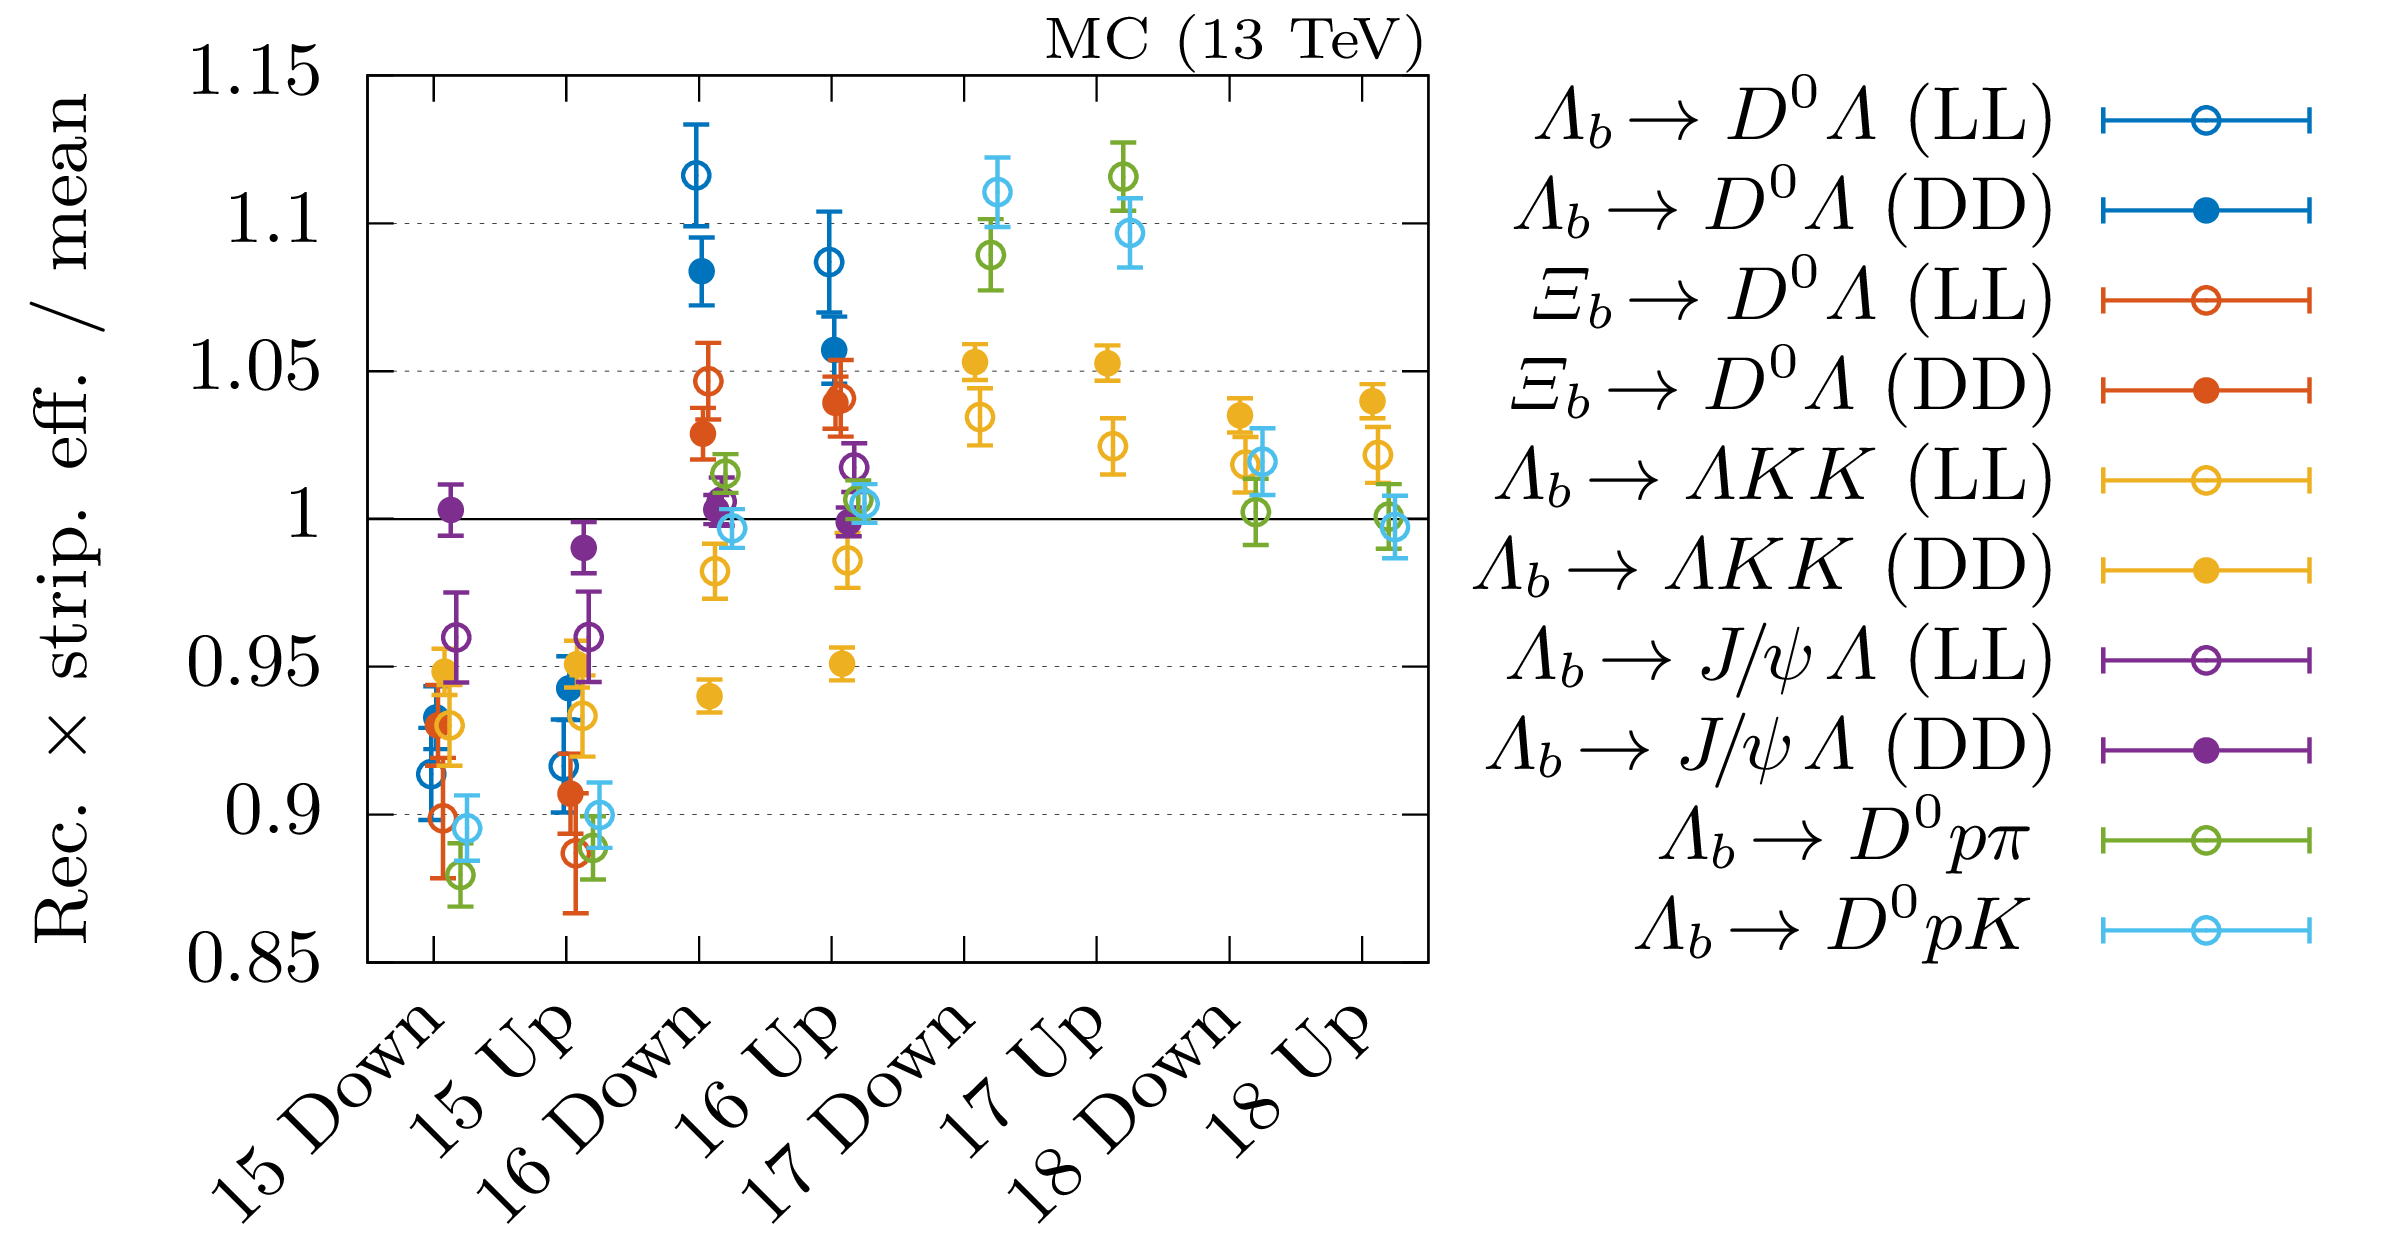
\includegraphics[scale=1.]{stripeff/effs.png}
    \caption{Combined reconstruction and \gls{stripping} efficiency for the decays under consideration. For the sake of brevity, magnet polarities are referred to as \textit{Down} and \textit{Up} for mag.\ down and mag.\ up, respectively. In order to compensate for their wide spread, each value is normalized to the respective weighted mean of each decay for the full available data set. (Not all decays are simulated for the years 2017 and 2018.) For example $y \approx 0.95$ for \decay{\Lb}{\Lz\kaon\kaon} (DD) at $x=$ 15 Down reads as a 5\,\% deviation from the weighted mean of all simulated \decay{\Lb}{\Lz\kaon\kaon} decays with \gls{DD} tracks, where $x$ and $y$ refer to the abscissa and ordinate, respectively.}
    \label{fig:stripeff_effs}
\end{figure}
The efficiencies shown in Fig.~\ref{fig:stripeff_effs} are normalized to the respective weighted mean of each decay for the full available data set (still separated w.r.t.\ the track types \gls{LL} and \gls{DD}) where we find the weighted mean $\varepsilon$ of $N$ efficiencies $p_i = n_i / N_i$ by calculating\footnote{In order to unfold relative deviations among different \gls{mc} simulated decays from biases introduced by fit models, we use \gls{truthmatched} events for this task.}
\begin{equation*}
    \varepsilon = \frac{\sum_i^N w_i \, p_i \, \varepsilon_{\text{gen},i}}{\sum_i^N w_i} \,,
\end{equation*}
where $w_i$ is the inverse sum in quadrature of the uncertainty of the generator cut efficiency $\sigma_{\text{gen},i}$ and the respective binomial uncertainty
\begin{equation*}
    w_i = \sigma_i^{-2} = \left(\sigma_{\text{gen},i}^2 + \frac{p_i (1 - p_i)}{N_i} \right)^{-1}.
\end{equation*}
Several things in Fig.~\ref{fig:stripeff_effs} are striking:
\begin{itemize}
    \item The discrepancy between simulated \decay{\Lb}{\Dz\Lz} and \decay{\Xibz}{\Dz\Lz} decays is larger than anticipated: The kinematics of both topologically identical decays should be very similar such that the deviation was more likely introduced by the various updates to the simulation framework (\texttt{Sim09c} $\to$ \texttt{Sim09h/g}). Therefore, we take simulated \decay{\Xibz}{\Dz\Lz} decays as the better proxy of genuine \decay{\Lb}{\Dz\Lz} decays than the dedicated \decay{\Lb}{\Dz\Lz} simulation for determining the combined generator cut and stripping efficiency.
    \item The efficiency drop for $\decay{\Lb}{\Dz\proton\Ph^-}$ for the year 2018: For the present analysis this drop affects \decay{\Lb}{\Dz\proton\pim} and stays unclear. For comparison we added the efficiency of \gls{mc} simulated \decay{\Lb}{\Dz\proton\Km} and \decay{\Lb}{\Lz\Kp\Km} where the drop is only visible for the former, hinting towards a correlation with the \Dz meson.
    \item The difference between \gls{LL} and \gls{DD} tracks is compatible for \decay{\Lb}{\jpsi\Lz} and \decay{\Lb}{\Lz\Kp\Km}: Even though the detector response for the former can be very different due to the dimuon pair in the final state, the difference between the track types of the \Lz daughters should be similar for the former and the latter. Further, we see that the variation of \gls{DD} tracks is smaller than for \gls{LL} tracks in both cases for the years 2015 and 2016.
    \item Similarly, the double ratio of \decay{\Lb}{\Dz\Lz} and \decay{\Xibz}{\Dz\Lz} and both track types is compatible with one. Hence, the ratio of the products of reconstruction and \gls{stripping} efficiency for \decay{\Lb}{\Dz\Lz} and \decay{\Xibz}{\Dz\Lz} does not depend on the track type in good approximation. 
\end{itemize}
The observed deviations do come with uncertainties and pinpointing exact causes is not possible.
When reliable values of the efficiencies are needed, we will therefore add a 10\,\% uncertainty to compensate for deviations that where introduced in the \gls{mc} simulated events but do not have any counterpart in recorded data.
This is a conservative approximation and will likely, based on the presented study, cover the true deviation.

%\section{Suppression Factors}
%\label{sec:stripeff_sups}
Taking the ratios of the combined reconstruction and \gls{stripping} efficiency of two \Lb decay modes gives access to suppression factors up to the \gls{stripping} process.
There are two relevant cases, first the relative suppression of \decay{\Lb}{\Dz\proton\pim} and \decay{\Lb}{\Dz\Lz}, needed for estimating the relative branching fraction of both, and secondly, the suppression of physical background contributions of \decay{\Lb}{\Dz\proton\pim} and \decay{\Lb}{\Lz\Kp\Km} in the invariant mass of \Dz and \Lz candidates.

For estimating the former, we use \gls{mc} simulated \decay{\Lb}{\Dz\proton\pim} events, reconstructed as \decay{\Lb}{\Dz\proton\pim}, and \gls{mc} simulated \decay{\Xib}{\Dz\Lz} events, reconstructed as \decay{\Lb}{\Dz\Lz} (the difference between reconstructed \Lb and \Xib is only the name tag).
The ratio as a function of different simulation conditions and track types of the \Lz daughters is shown in Fig.~\ref{fig:stripeff_Dzppi_vs_DzLz}.
\begin{figure}[htbp]
    \centering
    \begin{subfigure}{.49\textwidth}
        \centering
        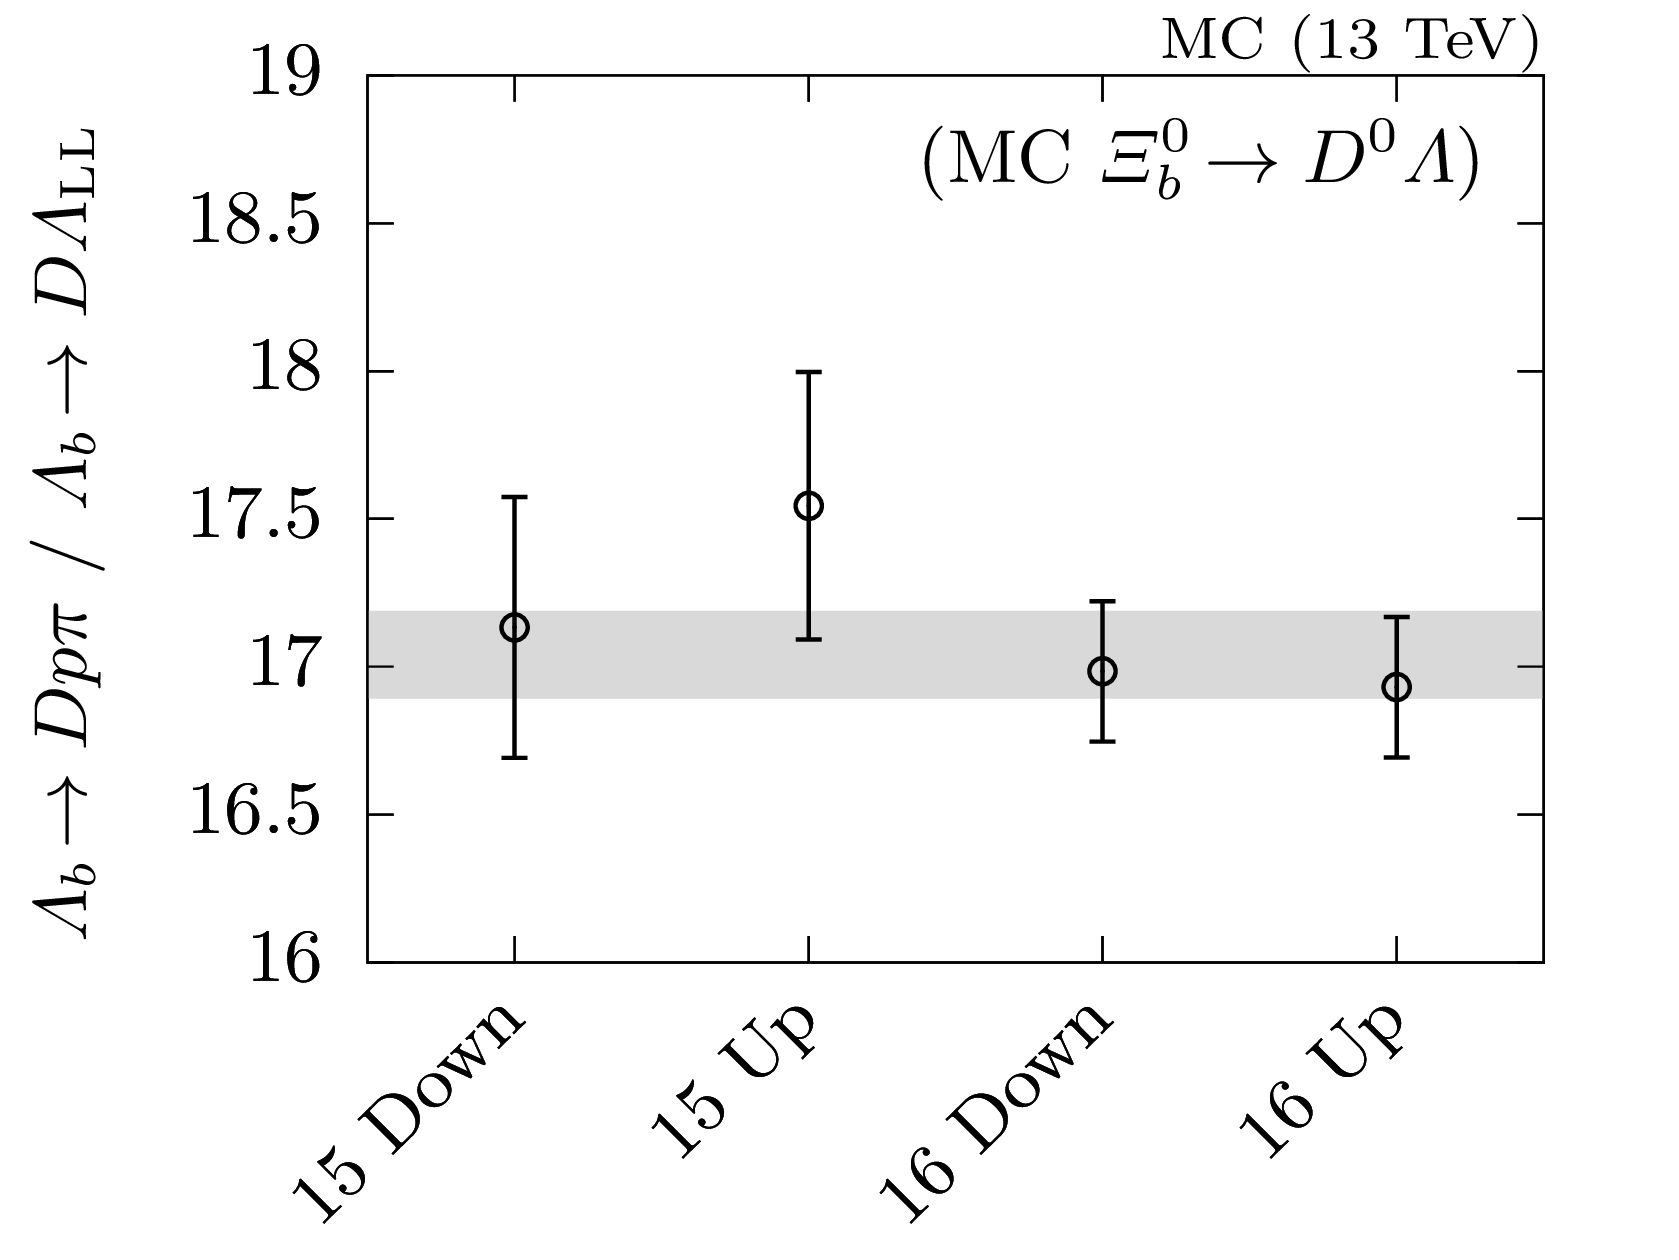
\includegraphics[scale=1.]{stripeff/ratio_Lb2Dzppi_Xib2DzLz_LL.png}
        \caption{\Lz reconstructed with \gls{LL} tracks}
    \end{subfigure}
    \begin{subfigure}{.49\textwidth}
        \centering
        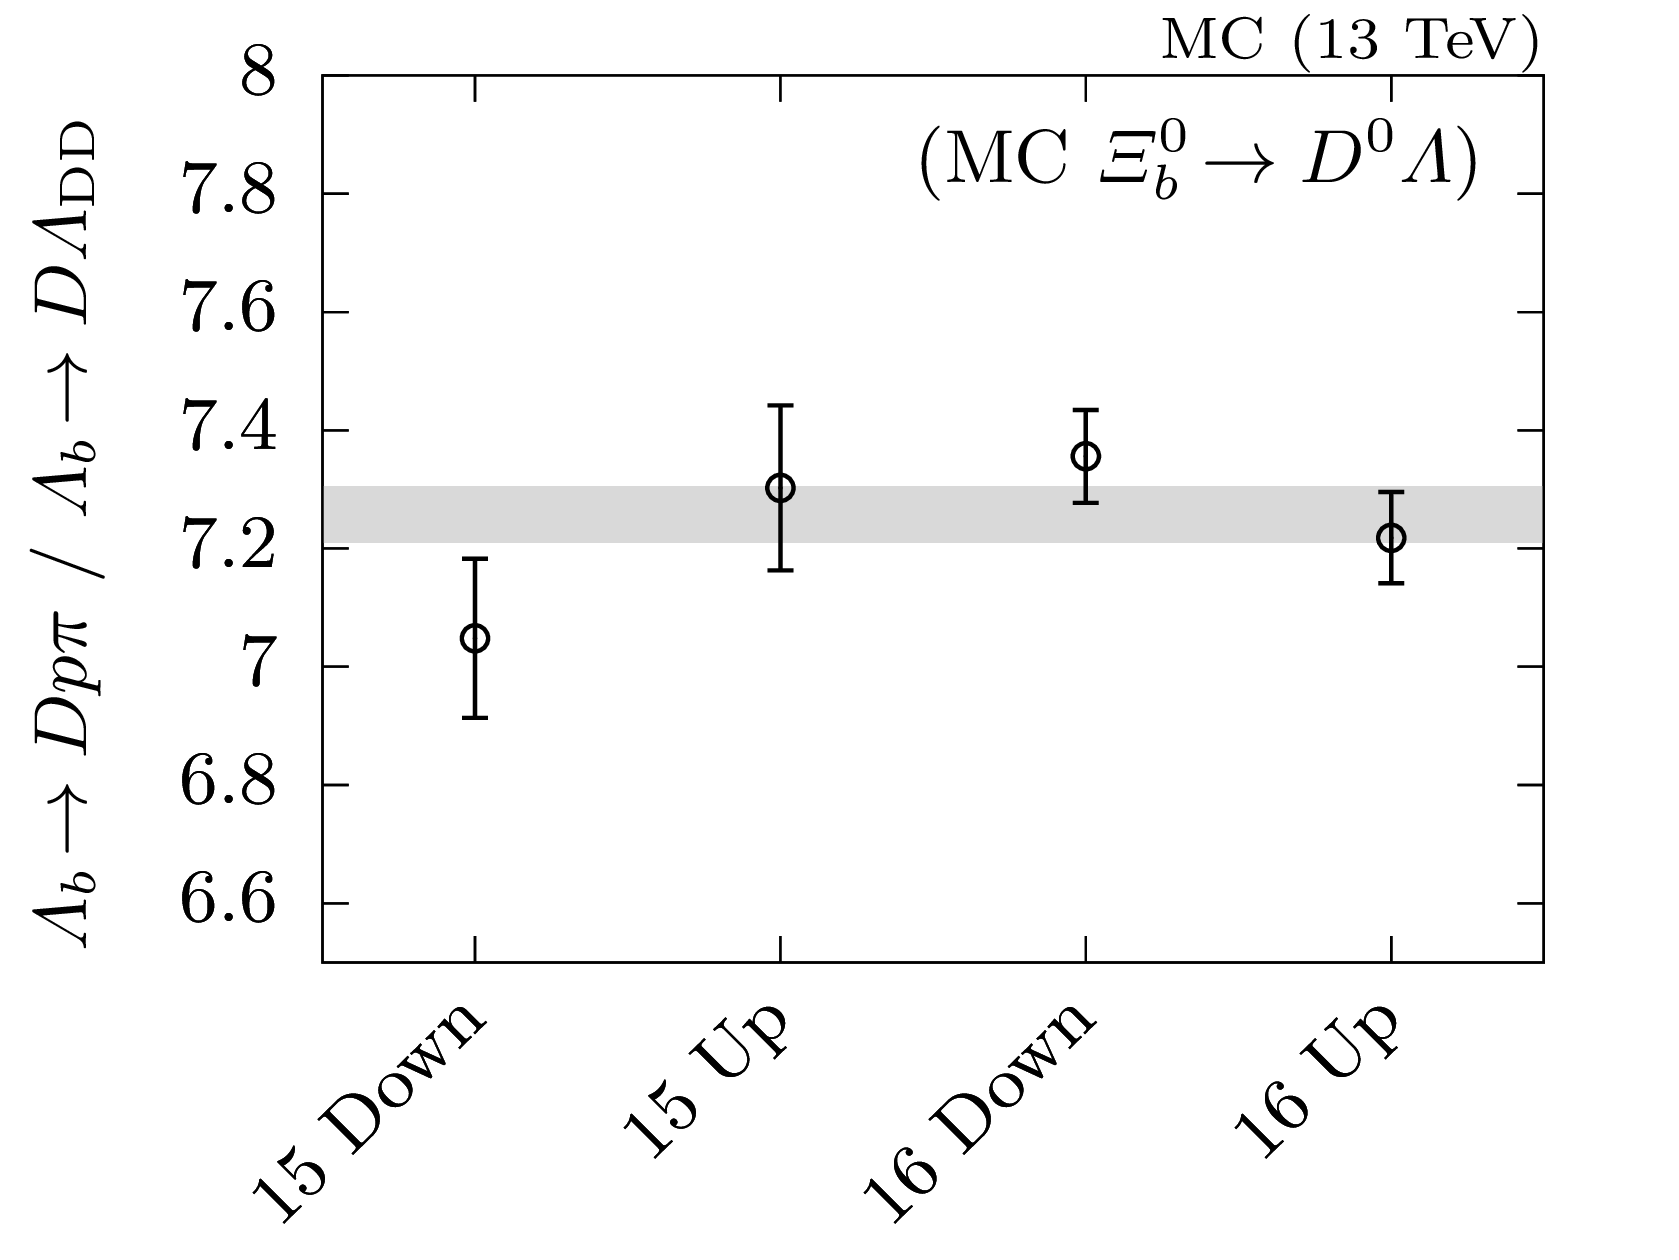
\includegraphics[scale=1.]{stripeff/ratio_Lb2Dzppi_Xib2DzLz_DD.png}
        \caption{\Lz reconstructed with \gls{DD} tracks}
    \end{subfigure}
    \caption{Ratio of the combined reconstruction and \gls{stripping} efficiency of \decay{\Lb}{\Dz\proton\pim} and \decay{\Lb}{\Dz\Lz} where we used \decay{\Xib}{\Dz\Lz} simulated decays as a proxy for the latter and differentiate between the track type of the \Lz daughters. The weighted means (grey box) are $17.04(15)$ and $7.26(5)$ for \gls{LL} tracks (left) and \gls{DD} tracks (right), respectively.}
    \label{fig:stripeff_Dzppi_vs_DzLz}
\end{figure}
The weighted means are $17.04(15)$ and $7.26(5)$ for \gls{LL} and \gls{DD} tracks, respectively.

The suppression factor $s$ of the background contribution of \decay{\Lb}{\Dz\proton\pim} in the invariant mass $m(\Dz\Lz)$ is only relevant for \gls{LL} tracks and is given by the ratio of the combined reconstruction and \gls{stripping} efficiency $\varepsilon$ of simulated \decay{\Lb}{\Dz\proton\pim} decays when reconstructed as \Dz\proton\pim and \Dz\Lz.
This suppression factor $s$ reduces the amount $n$ of reconstructed \decay{\Lb}{\Dz\proton\pim} decays, determined by an appropriate fitting technique in recorded data\footnote{In particular this means $n \neq \texttt{\#DTT}$ as used in Eq.~\eqref{eq:stripeff_defeps}.},
\begin{equation*}
    n / s = \left. n \middle/ \frac{\varepsilon\!\left( \decay{\Lb}{\Dz\proton\pim} \rightsquigarrow \Dz\proton\pim \right)}{\varepsilon\!\left( \decay{\Lb}{\Dz\proton\pim} \rightsquigarrow \Dz\Lz \right)} \right.,
\end{equation*}
where $\rightsquigarrow$ indicates the reconstruction state, hence $n/s$ is the expected amount of background contributions in $m(\Dz\Lz)$ up to the \gls{stripping} stage.

Since the recorded \decay{\Lb}{\Dz\proton\pim} sample allows a clean extraction of $n$, whereas the available samples of \decay{\Lb}{\Lz\Kp\Km} is noisier due to the smaller branching fraction and more pronounced background contributions (\cf{}~Ref.~\cite{LbToLzhh}), we also use $n$ for estimating the background contributions of charmless backgrounds.
We therefore take the results of the \gls{pdg},
\begin{align*}
    \frac{\BR(\decay{\Lb}{\Lz\Kp\Km})}{\BR(\decay{\Lb}{\Lc\pim})} &= (3.29 \pm 0.39) \times 10^{-3} \,, \\
    \frac{\BR(\decay{\Lb}{\Dz\proton\pim})}{\BR(\decay{\Lb}{\Lc\pim})} &= 0.13 \pm 0.01 \,,
\end{align*}
which are derived from the reported results of Refs.~\cite{LbToLzhh,LbToDzphAndLch}, and find
\begin{equation*}
    \kappa := \frac{\BR(\decay{\Lb}{\Dz\proton\pim})}{\BR(\decay{\Lb}{\Lz\Kp\Km})} = 40 \pm 6 \,,
\end{equation*}
assuming uncorrelated errors.
The latter assumption only holds for the statistical uncertainty strictly since both analyses are using different decay channels.
The systematic uncertainties though, do include a non-vanishing correlation, in particular because both analyses where carried out using data from the same detector.
Unfolding of correlated and uncorrelated fractions, however, is non-obvious and we will therefore use the conservative assumption of purely uncorrelated contributions which will slightly overestimate the total uncertainty.

Using $\kappa$ as the correction factor, the amount of reconstructed \decay{\Lb}{\Lz\Km\Kp} decays thus reads
\begin{equation*}
    n / s' = \left. n \middle/ \left( \kappa \times \frac{\varepsilon\!\left( \decay{\Lb}{\Dz\proton\pim} \rightsquigarrow \Dz\proton\pim \right)}{\varepsilon\!\left( \decay{\Lb}{\Lz\Km\Kp} \rightsquigarrow \Dz\Lz \right)} \times \frac{\BR(\decay{\Dz}{\Km\pip})}{\BR(\decay{\Lz}{\proton\pim})} \right) \right..
\end{equation*}
The values of $s$ and $s'$ are shown in Fig.~\ref{fig:stripeff_bkgsups}.
The weighted mean values are
\begin{subequations}
\label{eq:strip_effs_supfac}
\begin{align}
    s &= \num{24.4 \pm 0.4} \,, \\
    s' &= \begin{cases}
        \num{530 \pm 80} & \text{(\gls{LL})} \,, \\
        \num{210 \pm 30} & \text{(\gls{DD})} \,.
    \end{cases}
\end{align}
\end{subequations}

\begin{figure}[htbp]
    \centering
    \begin{subfigure}{.49\textwidth}
        \centering
        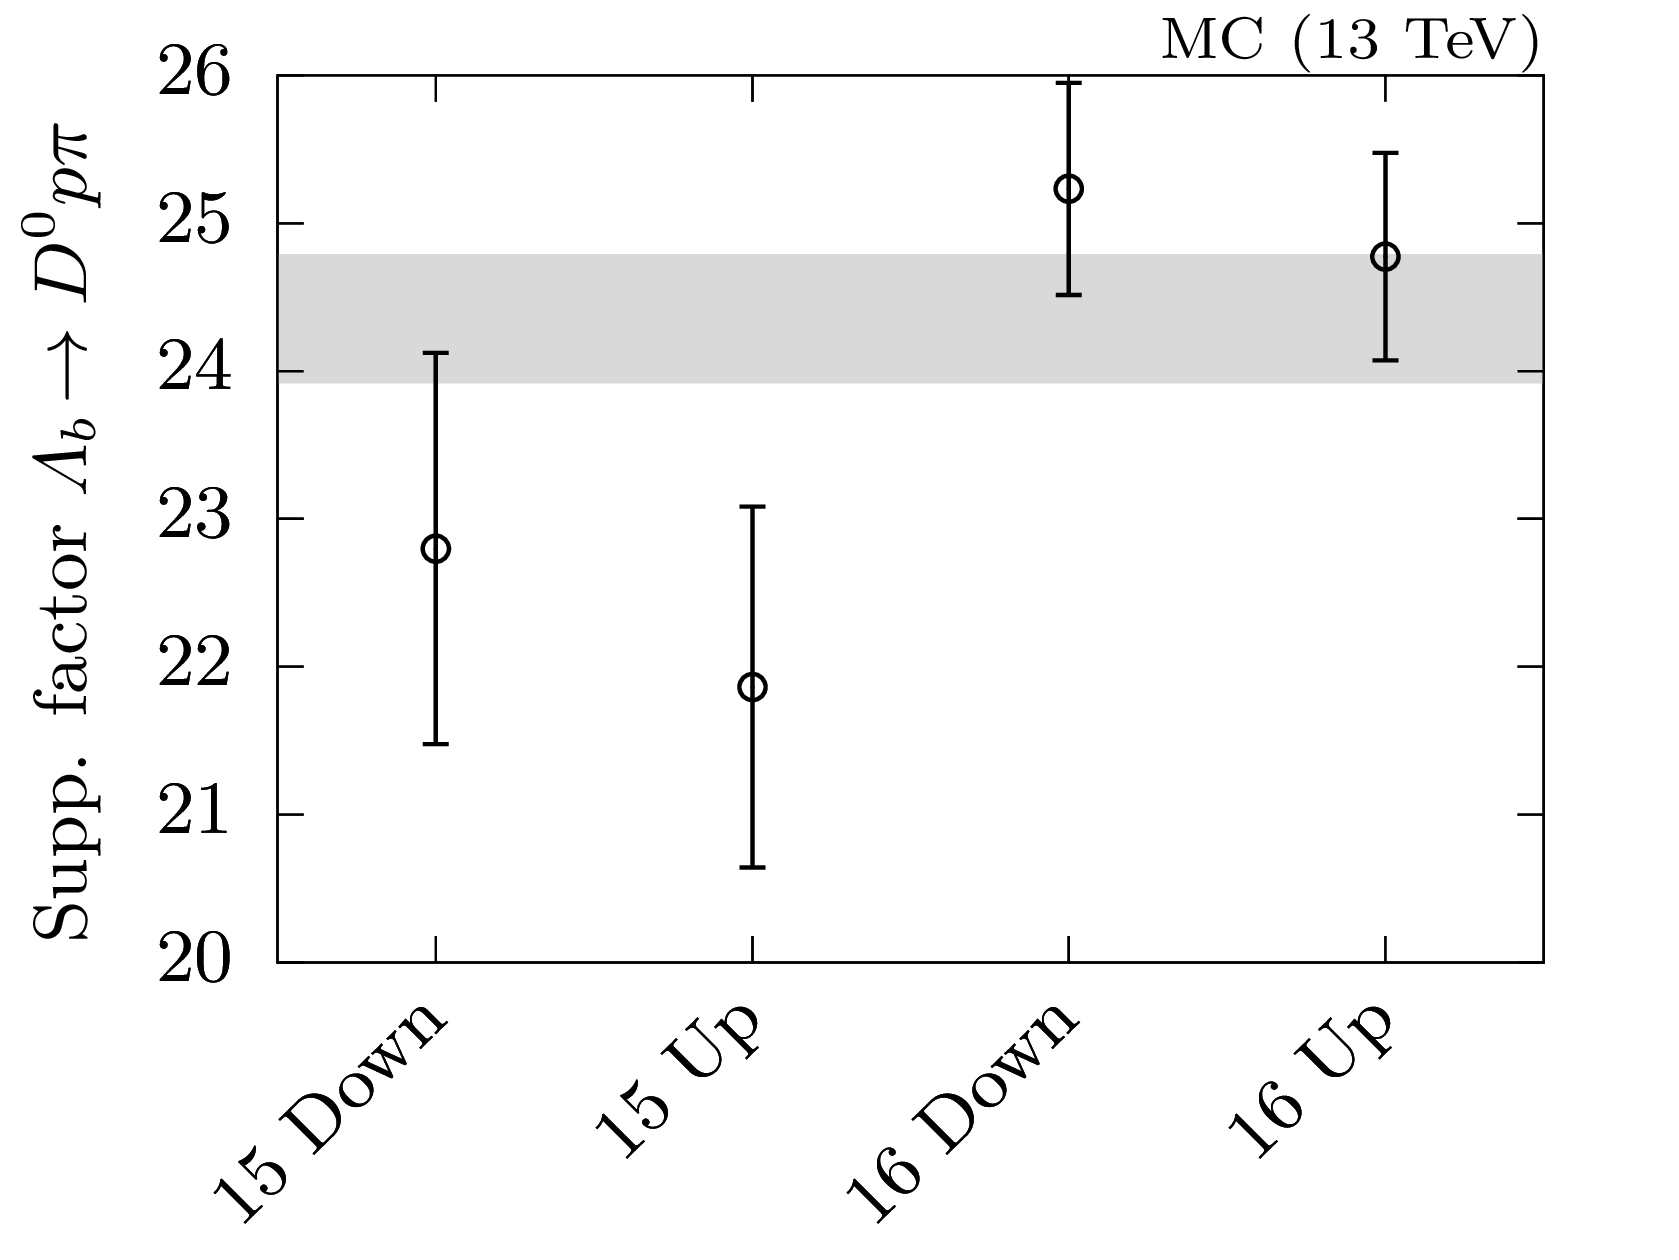
\includegraphics[scale=1.]{stripeff/bkgsup_Lb2Dzppi.png}
    \end{subfigure}
    \begin{subfigure}{.49\textwidth}
        \centering
        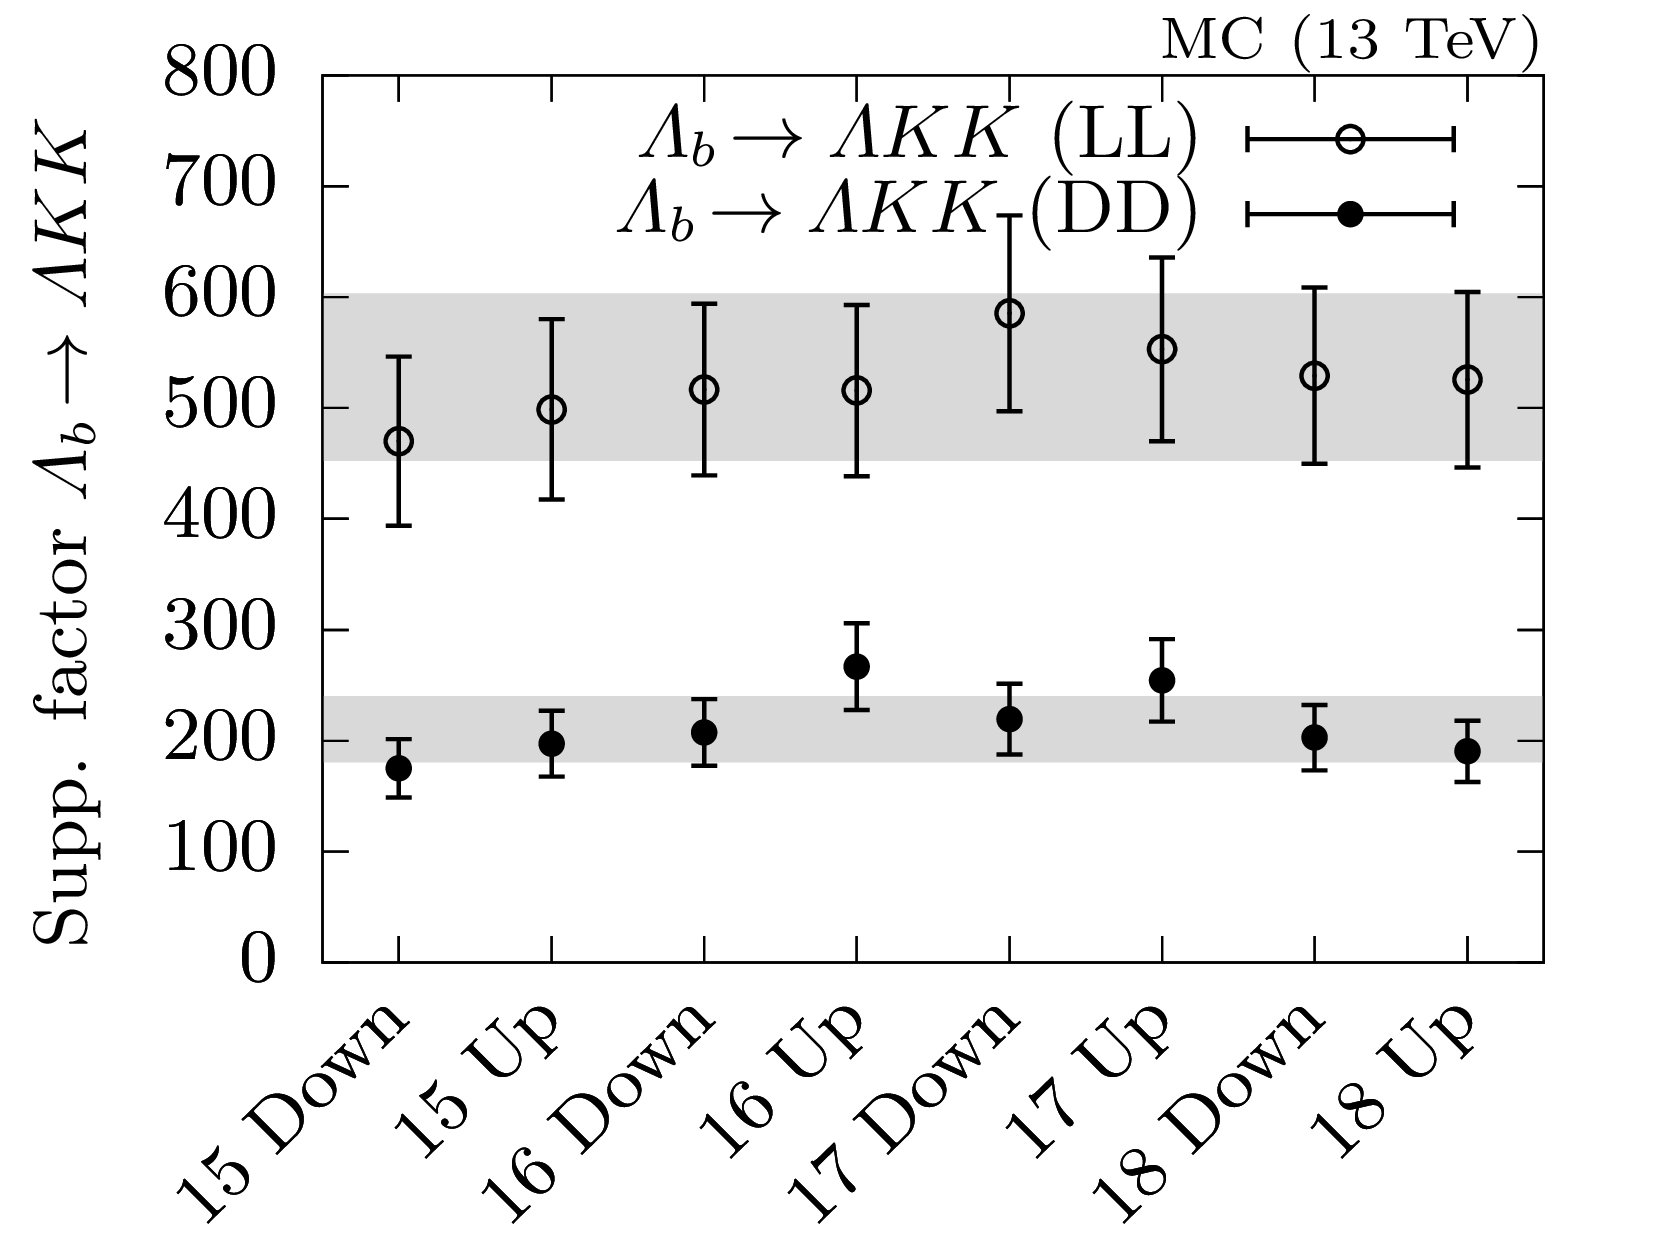
\includegraphics[scale=1.]{stripeff/bkgsup_Lb2LzKK.png}
    \end{subfigure}
    \caption{Suppression factors $s$ (left) and $s'$ (right) as defined in Eqs.~\eqref{eq:strip_effs_supfac} and respective weighted mean values (box).}
    \label{fig:stripeff_bkgsups}
\end{figure}


\chapter{Tuning MC Simulated Events by Determining Weights}
\label{chap:weights}
\chapquote{Light weight, baby!}{Ronnie Coleman.}
Monte Carlo (\gls{mc}) simulated events are a product from chaining various different software frameworks that use \gls{mc} methods to simulate the interaction and passage of particles through matter.
In particular the simulation of the passage of particles through matter highly relies on a high fidelity of the description of the detector assembly.
At the same time, a meticulous detector description slows down the simulation significantly and neither geometric, nor material specific properties of all sub-components can be known exactly.
For example, it is only possible to measure the magnetic field when the detector is partially disassembled.
The spatial distribution of the magnetic field of the assembled detector, which is a crucial input parameter for the particle simulation, thus already relies on error-prone estimations.
Further shortcomings are inaccurate alignments of detector units or imprecise physical input parameters, such as polarizations of initial state particles.

Some of these effects also limit the resolution of recorded data, but typically affect recorded data and \gls{mc} simulated events differently.
In the end, recorded data and \gls{mc} simulated events will never match exactly.
In particular, it is known that the distributions of transverse momentum \pt and pseudorapidity $\eta$ of simulated \Lb baryons can deviate significantly.

The idea of the following section is to weight simulated \Lb decays w.r.t.\ $\pt(\Lb)$ and $\eta(\Lb)$ in such a way that they match the distribution of recorded data.
When using the same set of selection requirements for simulated and recorded data, the extracted weights are selection independent scale factors (weights) that transform feature distributions of simulated \Lb decays to the corresponding distributions of recorded data.
In particular this means that those weights should not depend on kinematic properties, such as lifetime (and thus track type) of the respective daughters and grand-daughters of the \Lb, and thus are applicable also for different decay modes of the \Lb baryon.\footnote{We further use these weights to correct simulated \Xibz decays and incorporate deviations as a systematic uncertainty.}
In order to minimize trigger dependent deviations we only use \gls{lzero} \gls{tis} triggered \decay{\Lb}{\jpsi\Lz} events to extract weights and use them in a subsequent step for weighting \gls{mc} simulated \decay{\Lb/\Xibz}{\Dz\Lz} events.
%Using \gls{tis} instead of \gls{tos} triggered events minimized trigger dependent deviations of recorded and simulated data.

Properties that deviate between recorded and simulated data due to correlations with $\pt(\Lb)$ or $\eta(\Lb)$ will automatically improve with this technique.
We check this by comparing the momentum distribution $p(\Lb)$ of unweighted and weighted \gls{mc} simulated \decay{\Lb}{\jpsi\Lz} events. 

We try two different strategies for extracting weights.
The former minimizes deviations for both $\pt(\Lb)$ and $\eta(\Lb)$, whereas the latter uses $\pt(\Lb)$ only.
In the subsequent analysis we use the latter approach but incorporate deviations when using the weights obtained with the former strategy as a systematic uncertainty.
A description of the selection criteria used to increase the purity of the \decay{\Lb}{\jpsi\Lz} data samples is given in Sec.~\ref{sec:LbToJpsiLz_sel}.
A detailed explanation and discussion of the two different weighting schemes is given in Sec.~\ref{sec:LbToJpsiLz_w1} and Sec.~\ref{sec:LbToJpsiLz_w2}.
We further briefly motivate the use of sideband subtraction rather than relying on \gls{truthmatching} in Sec.~\ref{sec:LbToJpsiLz_tm_vs_ss}.

\section{The Decay \texorpdfstring{\decay{\Lb}{\jpsi\Lz}}{Λb → J/ψ Λ}}
\label{sec:LbToJpsiLz_sel}
The decay \decay{\Lb}{\jpsi\Lz} is a high statistics channel at \lhcb and was used there in the past to measure for example polarization effects \cite{LbToJpsiLz_polarization}.
Due to its large branching fraction this decay was one of the first discovered \Lb decay channels \cite{LbToJpsiLz_discovery} and measurements of the product of production fraction and branching fraction $f(\decay{\bquark}{\Lb}) \times \BR(\decay{\Lb}{\jpsi\Lz})$  at the \dzero and the \cdf collaborations~\cite{LbToJpsiLz_D0,LbToJpsiLz_CDF} are still used today for determining branching fractions from measurements of \Lb branching ratios.

%The quark transition in \decay{\Lb}{\jpsi\Lz} is \decay{\bquark}{\cquark\cquarkbar\squark} and is thus proportional to the product of \gls{ckm} matrix elements \Vcb \Vcss or $A\lambda^2$ in the \gls{wolfenstein}.
%In the Tab.~\ref{tab:LbToJpsiLz_qtransitions} below, we compare this amplitude in terms of \gls{ckm} matrix elements with the related modes \decay{\Bdsb}{\jpsi\KS}, as well as the respective decays for \decay{\Lb}{\Dz\Lz} and \decay{\Bdsb}{\Dz\KS}. 
%
%\begin{table}[htbp]
%    \centering
%    \caption{Quark transitions and \gls{ckm} matrix elements for \decay{\Lb}{\jpsi\Lz} and related modes.}
%    \label{tab:LbToJpsiLz_qtransitions}
%
%    \begin{tabular}{lll}
%    \toprule
%    Decay & Quark transition & \gls{ckm} matrix elements \\
%    \midrule
%    $\decay{\Lb}{\jpsi\Lz}$ & $\decay{(\bquark\uquark\dquark)}{(\cquark\cquarkbar)(\uquark\dquark\squark)}$ & $\Vcb \Vcss \sim A\lambda^2$ \\
%    $\decay{\Bdb}{\jpsi\KS}$ & $\decay{(\bquark\dquarkbar)}{(\cquark\cquarkbar)(\squark\dquarkbar)}$ & $\Vcb \Vcss \sim A\lambda^2$ \\
%    $\decay{\Bd}{\jpsi\KS}$ & $\decay{(\bquarkbar\dquark)}{(\cquark\cquarkbar)(\squarkbar\dquark)}$ & $\Vcbs \Vcs \sim A\lambda^2$ \\
%    $\decay{\Bsb}{\jpsi\KS}$ & $\decay{(\bquark\squarkbar)}{(\cquark\cquarkbar)(\squark\dquarkbar)}$ & $\Vcb \Vcds \sim A\lambda^3$ \\
%    $\decay{\Bs}{\jpsi\KS}$ & $\decay{(\bquarkbar\squark)}{(\cquark\cquarkbar)(\squarkbar\dquark)}$ & $\Vcbs \Vcd \sim A\lambda^3$ \\
%    \midrule
%    $\decay{\Lb}{\Dz\Lz}$ & $\decay{(\bquark\uquark\dquark)}{(\cquark\uquarkbar)(\uquark\dquark\squark)}$ & $\Vcb \Vuss \sim A\lambda^3$ \\
%    $\decay{\Lb}{\Dzb\Lz}$ & $\decay{(\bquark\uquark\dquark)}{(\cquarkbar\uquark)(\uquark\dquark\squark)}$ & $\Vub \Vcss \sim A\lambda^3$ \\
%    $\decay{\Xibz}{\Dz\Lz}$ & $\decay{(\bquark\uquark\squark)}{(\cquark\uquarkbar)(\uquark\dquark\squark)}$ & $\Vcb \Vuds \sim A\lambda^2$ \\
%    $\decay{\Xibz}{\Dzb\Lz}$ & $\decay{(\bquark\uquark\squark)}{(\cquarkbar\uquark)(\uquark\dquark\squark)}$ & $\Vub \Vcds \sim A\lambda^4$ \\
%    $\decay{\Bdb}{\Dz\KS}$ & $\decay{(\bquark\dquarkbar)}{(\cquark\uquarkbar)(\squark\dquarkbar)}$ & $\Vcb \Vuss \sim A\lambda^3$ \\
%    $\decay{\Bdb}{\Dzb\KS}$ & $\decay{(\bquark\dquarkbar)}{(\cquarkbar\uquark)(\squark\dquarkbar)}$ & $\Vub \Vcss \sim A\lambda^3$ \\
%    $\decay{\Bsb}{\Dz\KS}$ & $\decay{(\bquark\squarkbar)}{(\cquark\uquarkbar)(\squark\dquarkbar)}$ & $\Vcb \Vuds \sim A\lambda^2$ \\
%    $\decay{\Bsb}{\Dzb\KS}$ & $\decay{(\bquark\squarkbar)}{(\cquarkbar\uquark)(\squark\dquarkbar)}$ & $\Vub \Vcds \sim A\lambda^4$ \\
%    \bottomrule
%    \end{tabular}
%\end{table}
%
%Despite the fact that the \gls{ckm} matrix elements listed in Tab.~\ref{tab:LbToJpsiLz_qtransitions} do not take different production rates of the initial \bquark hadrons into account, which contribute non-negligible corrections due to differences in the fragmentation process of \bquark quarks to hadrons, these numbers show two things: \decay{\Lb}{\jpsi\Lz} is much less suppressed than \decay{\Lb}{\Dz\Lz}, whereas background contributions from \Bdb and \Bsb (\glspl{reflection}) are suppressed stronger.
%This makes \decay{\Lb}{\jpsi\Lz} a good candidate for systematic and calibration studies.

In the following we use $\decay{\Lb}{(\decay{\jpsi}{\mun\mup})(\decay{\Lz}{\proton\pim}})$ to extract weights for calibrating the \gls{mc} samples for \decay{\Lb}{\Dz\Lz}.
In order to minimize systematic uncertainties introduced by imprecise simulated trigger responses, only \gls{lzero} \gls{tis} triggered events are used.
In the following we will outline the selection steps which we divide into a preselection, a loose, and a tight selection.
%After applying the outlined selection requirements, we add a brief discussion about their efficiency and end with a short discussion about the distribution of the fit probability.

\subsection{Preselection}
\label{sec:LbToJpsiLz_presel}
We use the full recorded data set of \gls{runtwo} and the \gls{stripping} versions listed in Tab.~\ref{tab:LbToJpsiLz_vstripping}.
Despite their different naming, there are no major differences between different \gls{stripping} versions for the involved \gls{stripping} lines.
\begin{table}[htbp]
    \centering
    \caption{\Gls{stripping} and Reco versions used for reconstructing \decay{\Lb}{\jpsi\Lz}.}
    \label{tab:LbToJpsiLz_vstripping}

    \begin{tabular}{lll}
        \toprule
        Year & \Gls{stripping} & Reco \\
        \midrule
        2015 & \texttt{24r1} & \texttt{15a} \\
        2016 & \texttt{28r1} & \texttt{16} \\
        2017 & \texttt{29r2} & \texttt{17} \\
        2018 & \texttt{34} & \texttt{18} \\
        \bottomrule
    \end{tabular}
\end{table}
Mother particles are reconstructed from daughter particles that passed dedicated \textit{combination} selections.
Properties of the reconstructed mother particle are refined through the vertex fit procedure (no advanced constraints, such as mass or \gls{pv} constraints, are applied) and are subject to dedicated \textit{mother} selections, whereas properties of the respective daughter particles are not updated for subsequent selection steps.
%We use the results of the \gls{stripping} line \texttt{Stripping\-BetaS\-Lambdab2JpsiLambda\-Unbiased\-Line} and refine the \Lb selection with selection steps taken from the \gls{stripping} line \texttt{Stripping\-Lb2D0Lambda0\-\{LL,DD\}\-D02HH\-Beauty2Charm\-Line}.
All selection criteria of the preselection step are listed in Tab.~\ref{tab:LbToJpsiLz_stripsel}.

\subsection{Loose Selection}
\label{sec:LbToJpsiLz_loosesel}
A decay tree fit is applied and the corresponding $\chi^2_\text{DTF}$ distribution\footnote{We will later find that this distribution does not exactly follow the distribution of a \textit{true} $\chi^2$-distribution. For the sake of brevity we will nevertheless refer to it as a $\chi^2_\text{DTF}$.} is used for discriminating combinatorial background.
The $\chi^2_\text{DTF}$ distribution has 8 degrees of freedom (\cf{}~Sec.~\ref{chap:apdx_dtf} for a more detailed discussion):
\begin{itemize}[itemsep=2pt,parsep=2pt]
    \item Mass constraint of \Lz and \jpsi: 2 \gls{dof}
    \item \Lz vertex constraint: 1 \gls{dof}
    \item \decay{\Lb}{\mup\mun\Lz} vertex constraint: 3 \gls{dof}
    \item \Lb \gls{pv} constraint: 2 \gls{dof}
\end{itemize}
The \gls{pv} constraint leverages an ordering of different \gls{pv} hypotheses (if available) w.r.t.\ the goodness of a respective \gls{dtf} (in terms of $\chi^2_\text{DTF}$).
We use this to select only candidates corresponding to the best \gls{pv} hypothesis for the following steps.

The selection criteria of the loose selection are shown in Tab.~\ref{tab:LbToJpsiLz_loosesel} and are grouped into five categories:
Category 1 reduces combinatorial background in the signal region, category 2 ensures disjunct samples w.r.t.\ the track types \gls{LL} and \gls{DD}, and category 3 reduces disk consumption.
The momentum requirements for the final state particles in category 1 are motivated by the fact that particles do have to have a minimal velocity to emit Cherenkov radiation.
Cherenkov light is instrumented in the \gls{rich} detectors for the particle identification at \lhcb.
Particle identification (\gls{pid}) below this threshold and above $\gtrapprox 150\,$\gevc is ineffective.
(These selection requirements supersede the implicit cut-off of $p > 1.4\,$\gevc due to magnet banding.)
The fiducial selection criteria (category 4) are a common choice for initial state particles at \lhcb.
These selections help to avoid known issues with the fidelity of the detector geometry description in the inner- and outermost regions and turned out to be a conservative choice when the overall statistic is sufficient.
Category 5 minimizes the effect of poorly described trigger in simulated data which could potentially introduce a systematic difference between recorded and simulated events.

\begin{table}[htbp]
    \caption{Selection criteria of loose selection used for reconstructing \decay{\Lb}{\jpsi\Lz}. The selections are grouped into five categories which are explained in Sec.~\ref{sec:LbToJpsiLz_loosesel}.}
    \label{tab:LbToJpsiLz_loosesel}

    \centering
    \begin{tabular}{llc}
        \toprule
        Particle & Selection & Category \\
        \midrule
        \proton & $9 \le p \le 150\,$\gevc & 1 \\
        \pion & $3 \le p \le 150\,$\gevc & 1 \\
        \midrule
        \Lz & decay length $\ge 0$ & 1 \\
        \Lz (\gls{LL}) & $z$-pos.\ of decay vertex $<0.5\,$m & 2 \\
        \Lz (\gls{DD}) & $z$-pos.\ of decay vertex $\ge 0.5\,$m & 2 \\
        \midrule
        \Lb & $5.47 \le m \le 5.77\,\gevcc$ & 3 \\
        \Lb & $2 \le \eta \le 4.5$ & 4 \\
        \Lb & $\pt \le 20\,\gevc$ & 4 \\
        \Lb & \gls{lzero} \gls{tis} events only & 5 \\
        \bottomrule
    \end{tabular}
\end{table}

The data samples are split w.r.t.\ the different track types of the \Lz daughters which are referred to as \gls{LL} and \gls{DD}.
%In light of the available statistic mixed states, such as LD tracks, are not taken into account.
%In Fig.~\ref{fig:mLbToJpsiLz_loosesel} we show the invariant mass of \Lb candidates, reconstructed from recorded data.
In order to optimize a \gls{fom}, we define a signal region spanning $5.58 \le m(\jpsi\Lz) \le 5.66\,\gevcc$.
Events outside this region (upper and lower sideband) are considered pure combinatorial background, whereas events inside the signal region are considered to be an admixture of signal and (combinatorial) background events.
Physical background processes are neglected in this part of the analysis since no visible contributions are visible in the invariant mass distributions.% shown in Fig.~\ref{fig:mLbToJpsiLz_loosesel}.

%\begin{figure}[htbp]
%    \centering
%    \begin{subfigure}[b]{.49\textwidth}
%        \centering
%        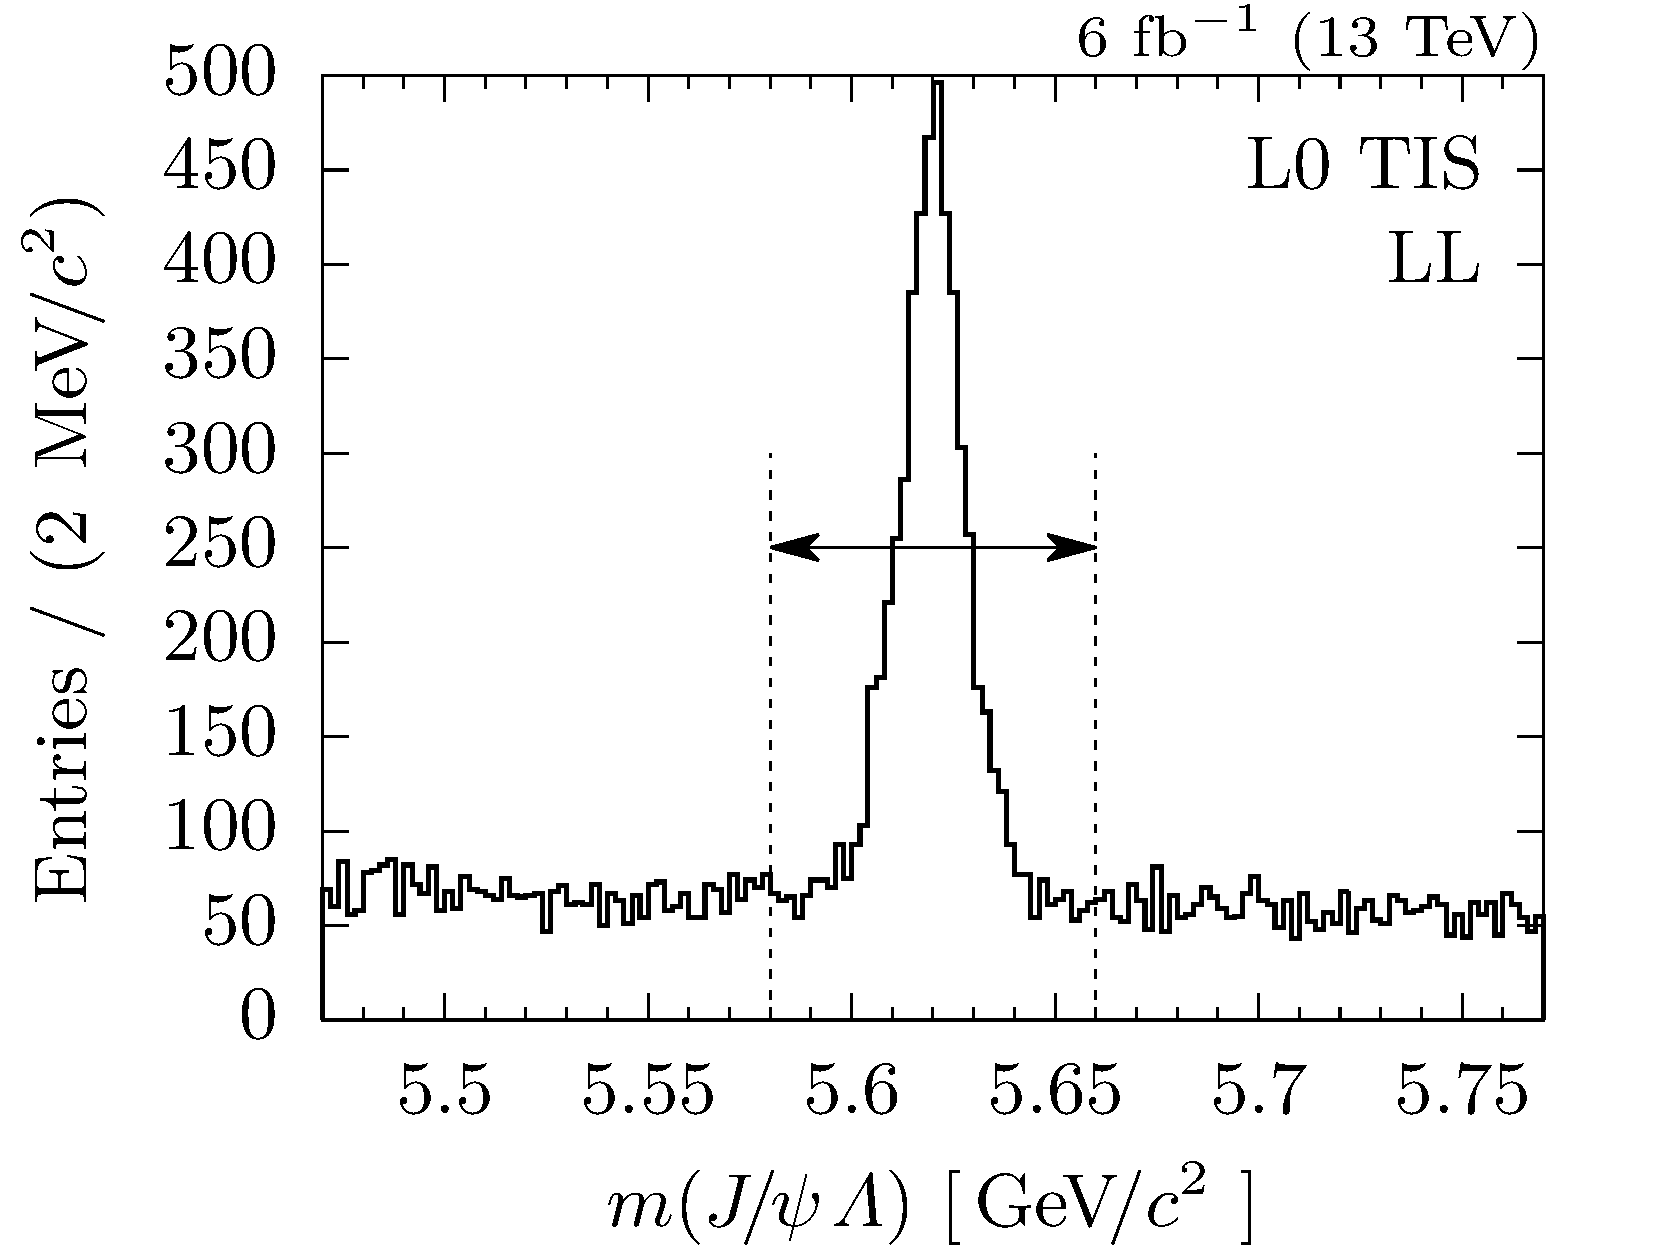
\includegraphics[scale=1.]{Lb2JpsiLz_weighting/hLbM_LL.png}
%        \caption{\Lz candidates rec.\ from \gls{LL} tracks}
%    \end{subfigure}
%    \begin{subfigure}[b]{.49\textwidth}
%        \centering
%        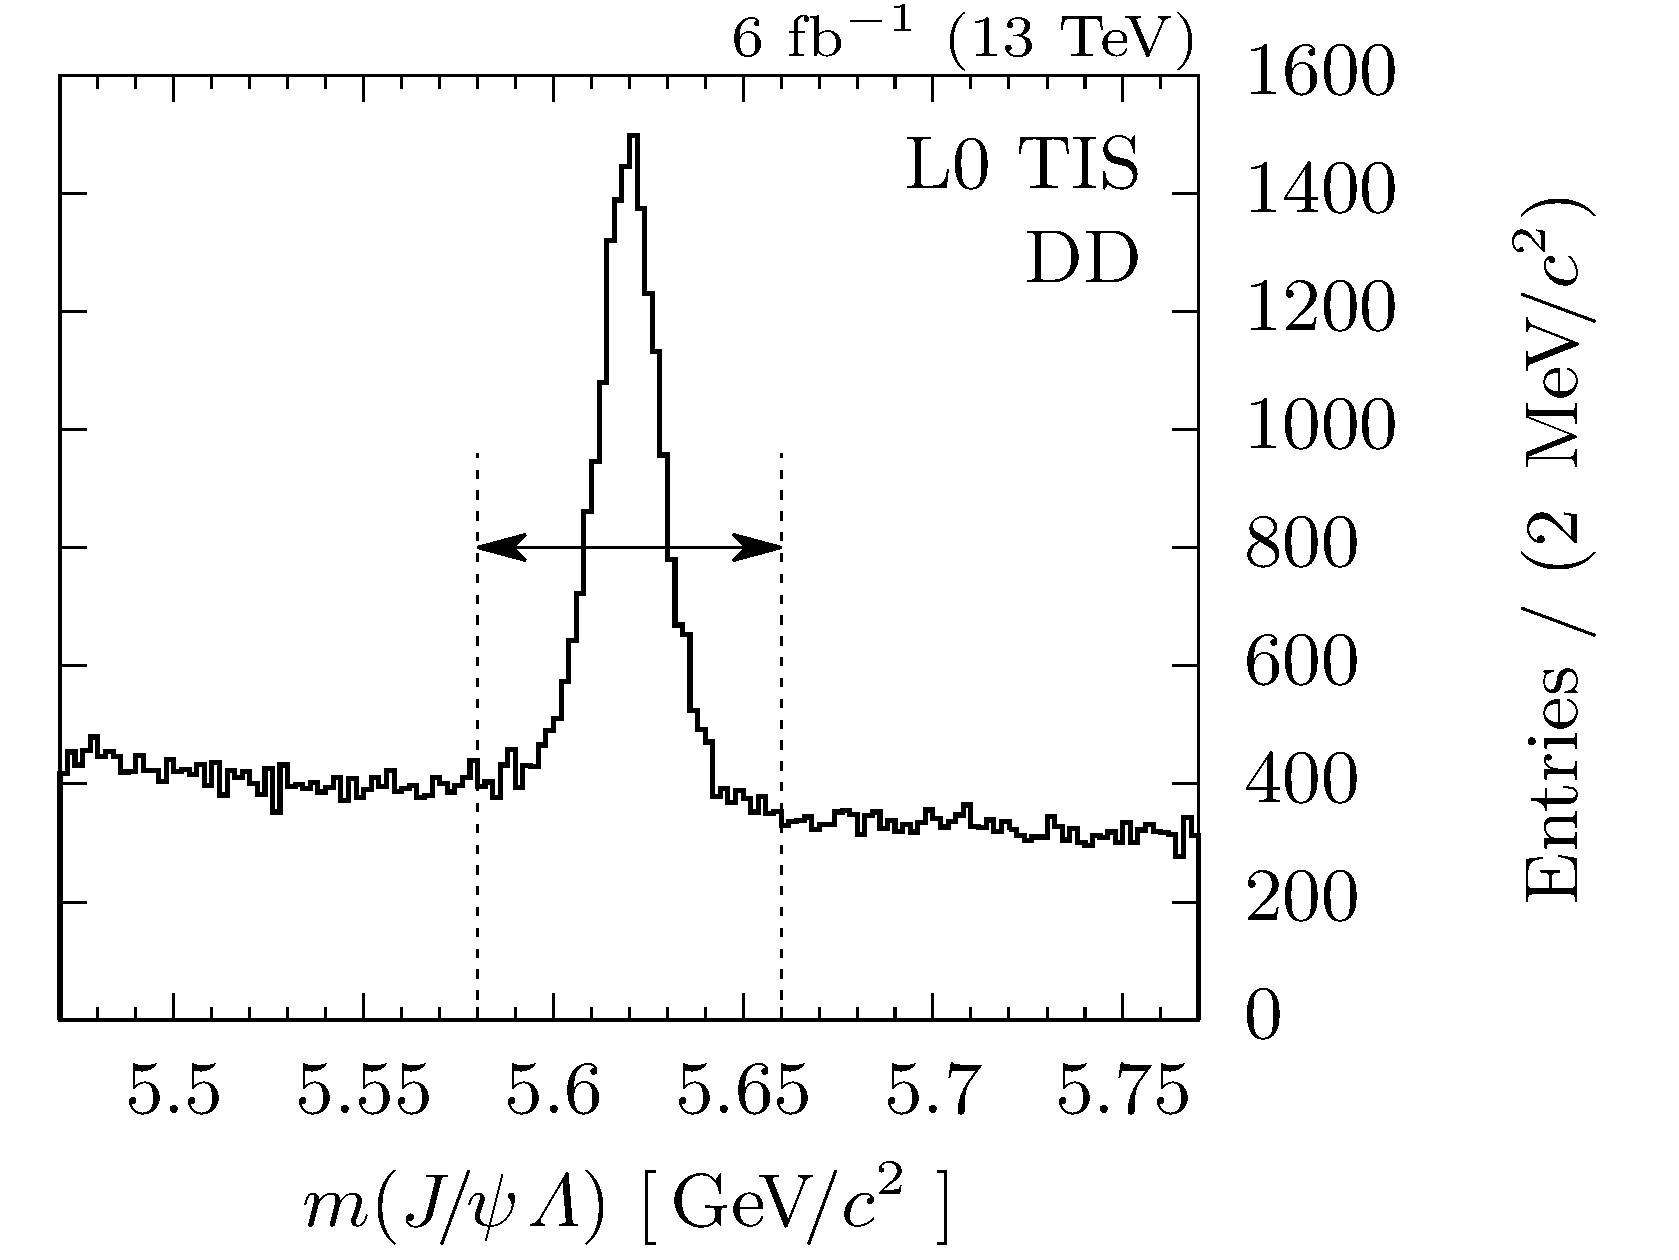
\includegraphics[scale=1.]{Lb2JpsiLz_weighting/hLbM_DD.png}
%        \caption{\Lz candidates rec.\ from \gls{DD} tracks}
%    \end{subfigure}
%    \caption{Combined invariant mass of \jpsi and \Lz candidates after loose selection from recorded data. (Including \gls{lzero} \gls{tis} only requirement.) The dashed lines indicate the \Lb signal region that is used for optimizing a \gls{fom} as part of the tight selection.}
%    \label{fig:mLbToJpsiLz_loosesel}
%\end{figure}

\subsection{Tight Selection}
The objective of the tight selection is to maximize the signal significance as the \gls{fom} for $n_\text{sig}$ signal events and $n_\text{bkg}$ background events in the defined signal region,
\begin{equation}
    \label{eq:fom_LbToJpsiLz}
    \mathrm{FoM} := \mathrm{FoM}(n_\text{sig}, n_\text{bkg}) = \frac{n_\text{sig}}{\sqrt{n_\text{sig} + n_\text{bkg}}} \,.
\end{equation}

The signal significance is maximized for selection requirements w.r.t.\ the $\chi^2_\text{DTF}$ distribution of the \gls{dtf} and the flight distance significance of the \Lz baryon, where the latter is defined as the flight distance $\mathrm{FD}(\Lz)$ over the corresponding standard deviation $u_\mathrm{FD}(\Lz)$ of the \Lz baryon,
\begin{equation*}
    \text{\Lz flight dist. sig.} := \frac{\mathrm{FD}(\Lz)}{u_\mathrm{FD}(\Lz)} \,.
\end{equation*}

The cumulative distributions for both of these features are shown in Fig.~\ref{fig:chi2dtf_LbToJpsiLz} and Fig.~\ref{fig:LzFDs_LbToJpsiLz} for recorded data in the defined signal region and \gls{mc} simulated events.
The cumulative distribution of $\chi^2_\text{DTF}$ indicates a strong separation power between signal and background events, whereas the cumulative distributions of the \Lz flight distance only show minor differences between recorded data and simulated events, hinting towards a low background contamination for the \Lz baryon, \ie{}, the background in $m(\jpsi\Lz)$ predominantly consists of combinatorial background events with genuine \Lz baryons.

\begin{figure}[htbp]
    \centering
    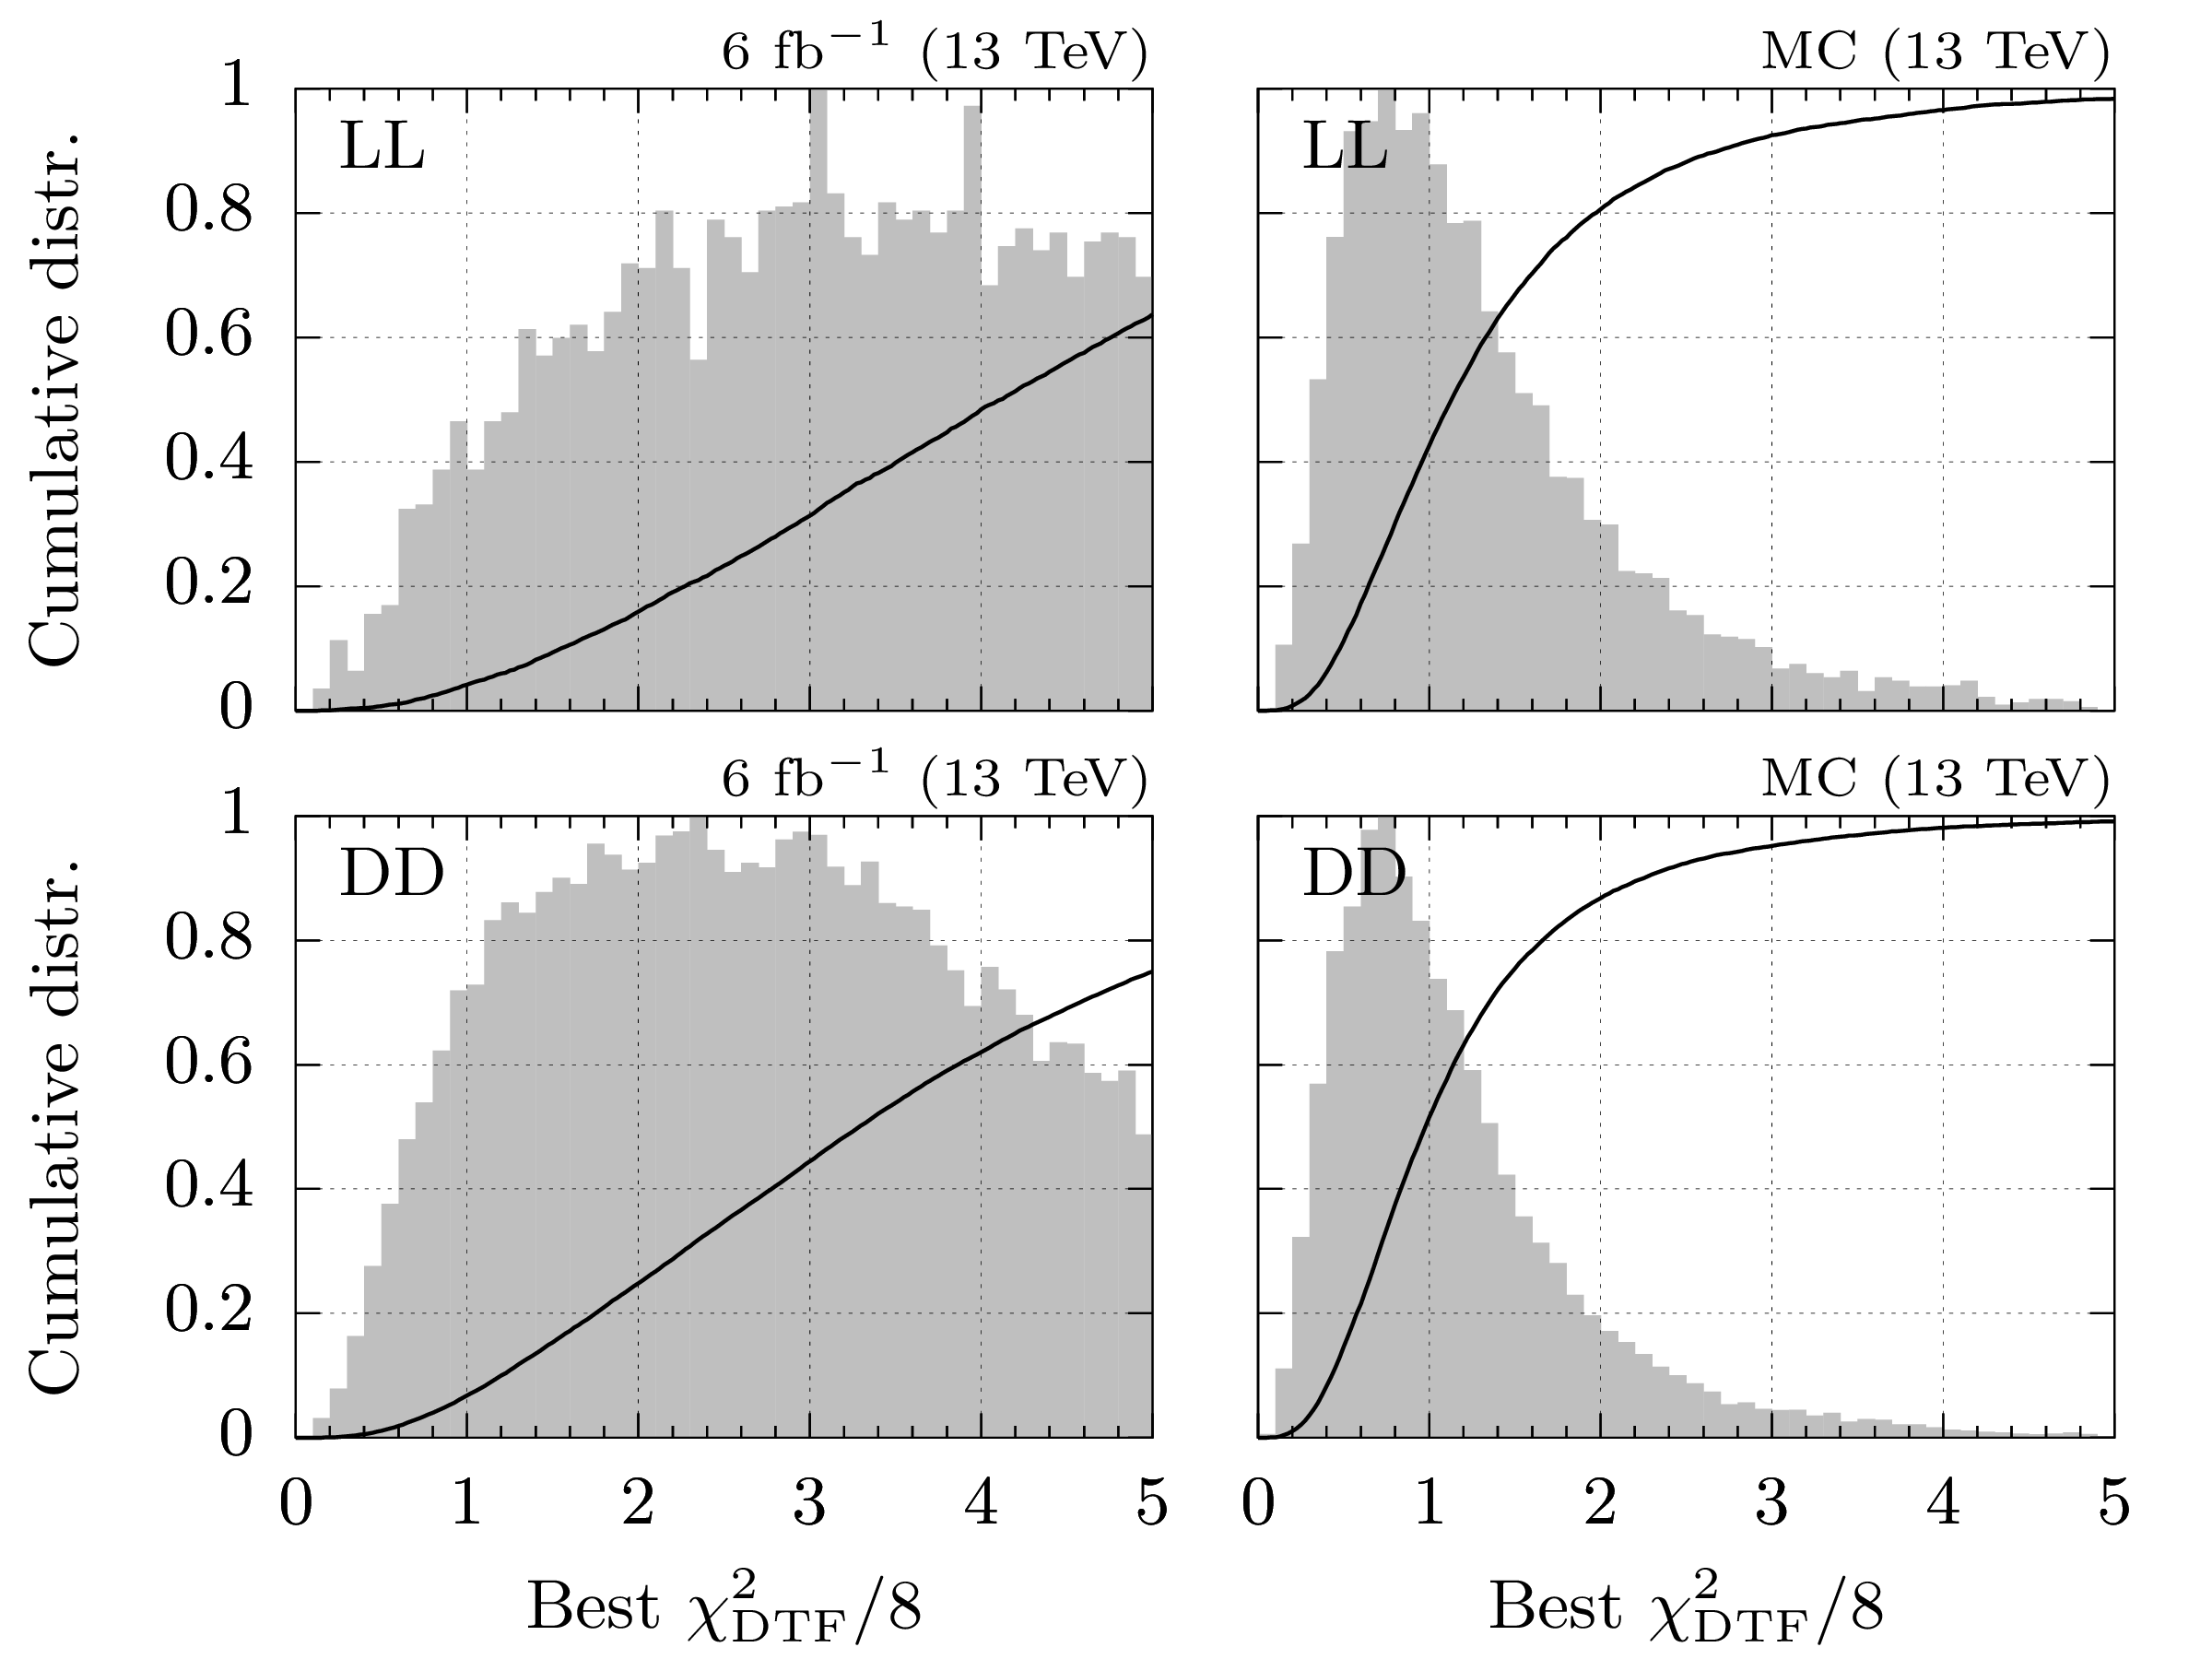
\includegraphics[scale=1.]{Lb2JpsiLz_weighting/chi2.png}
    \caption{Cumulative distribution (solid line) of the $\chi^2_\text{DTF}$ distribution over \gls{dof} for different track types (top and bottom), and for recorded data in the defined signal regions (left) and \gls{truthmatched} simulated events in the signal region (right). The gray shaded areas indicate the corresponding distributions of $\chi^2_\text{DTF}/\mathrm{\gls{dof}}$.}
    \label{fig:chi2dtf_LbToJpsiLz}
\end{figure}

\begin{figure}[htbp]
    \centering
    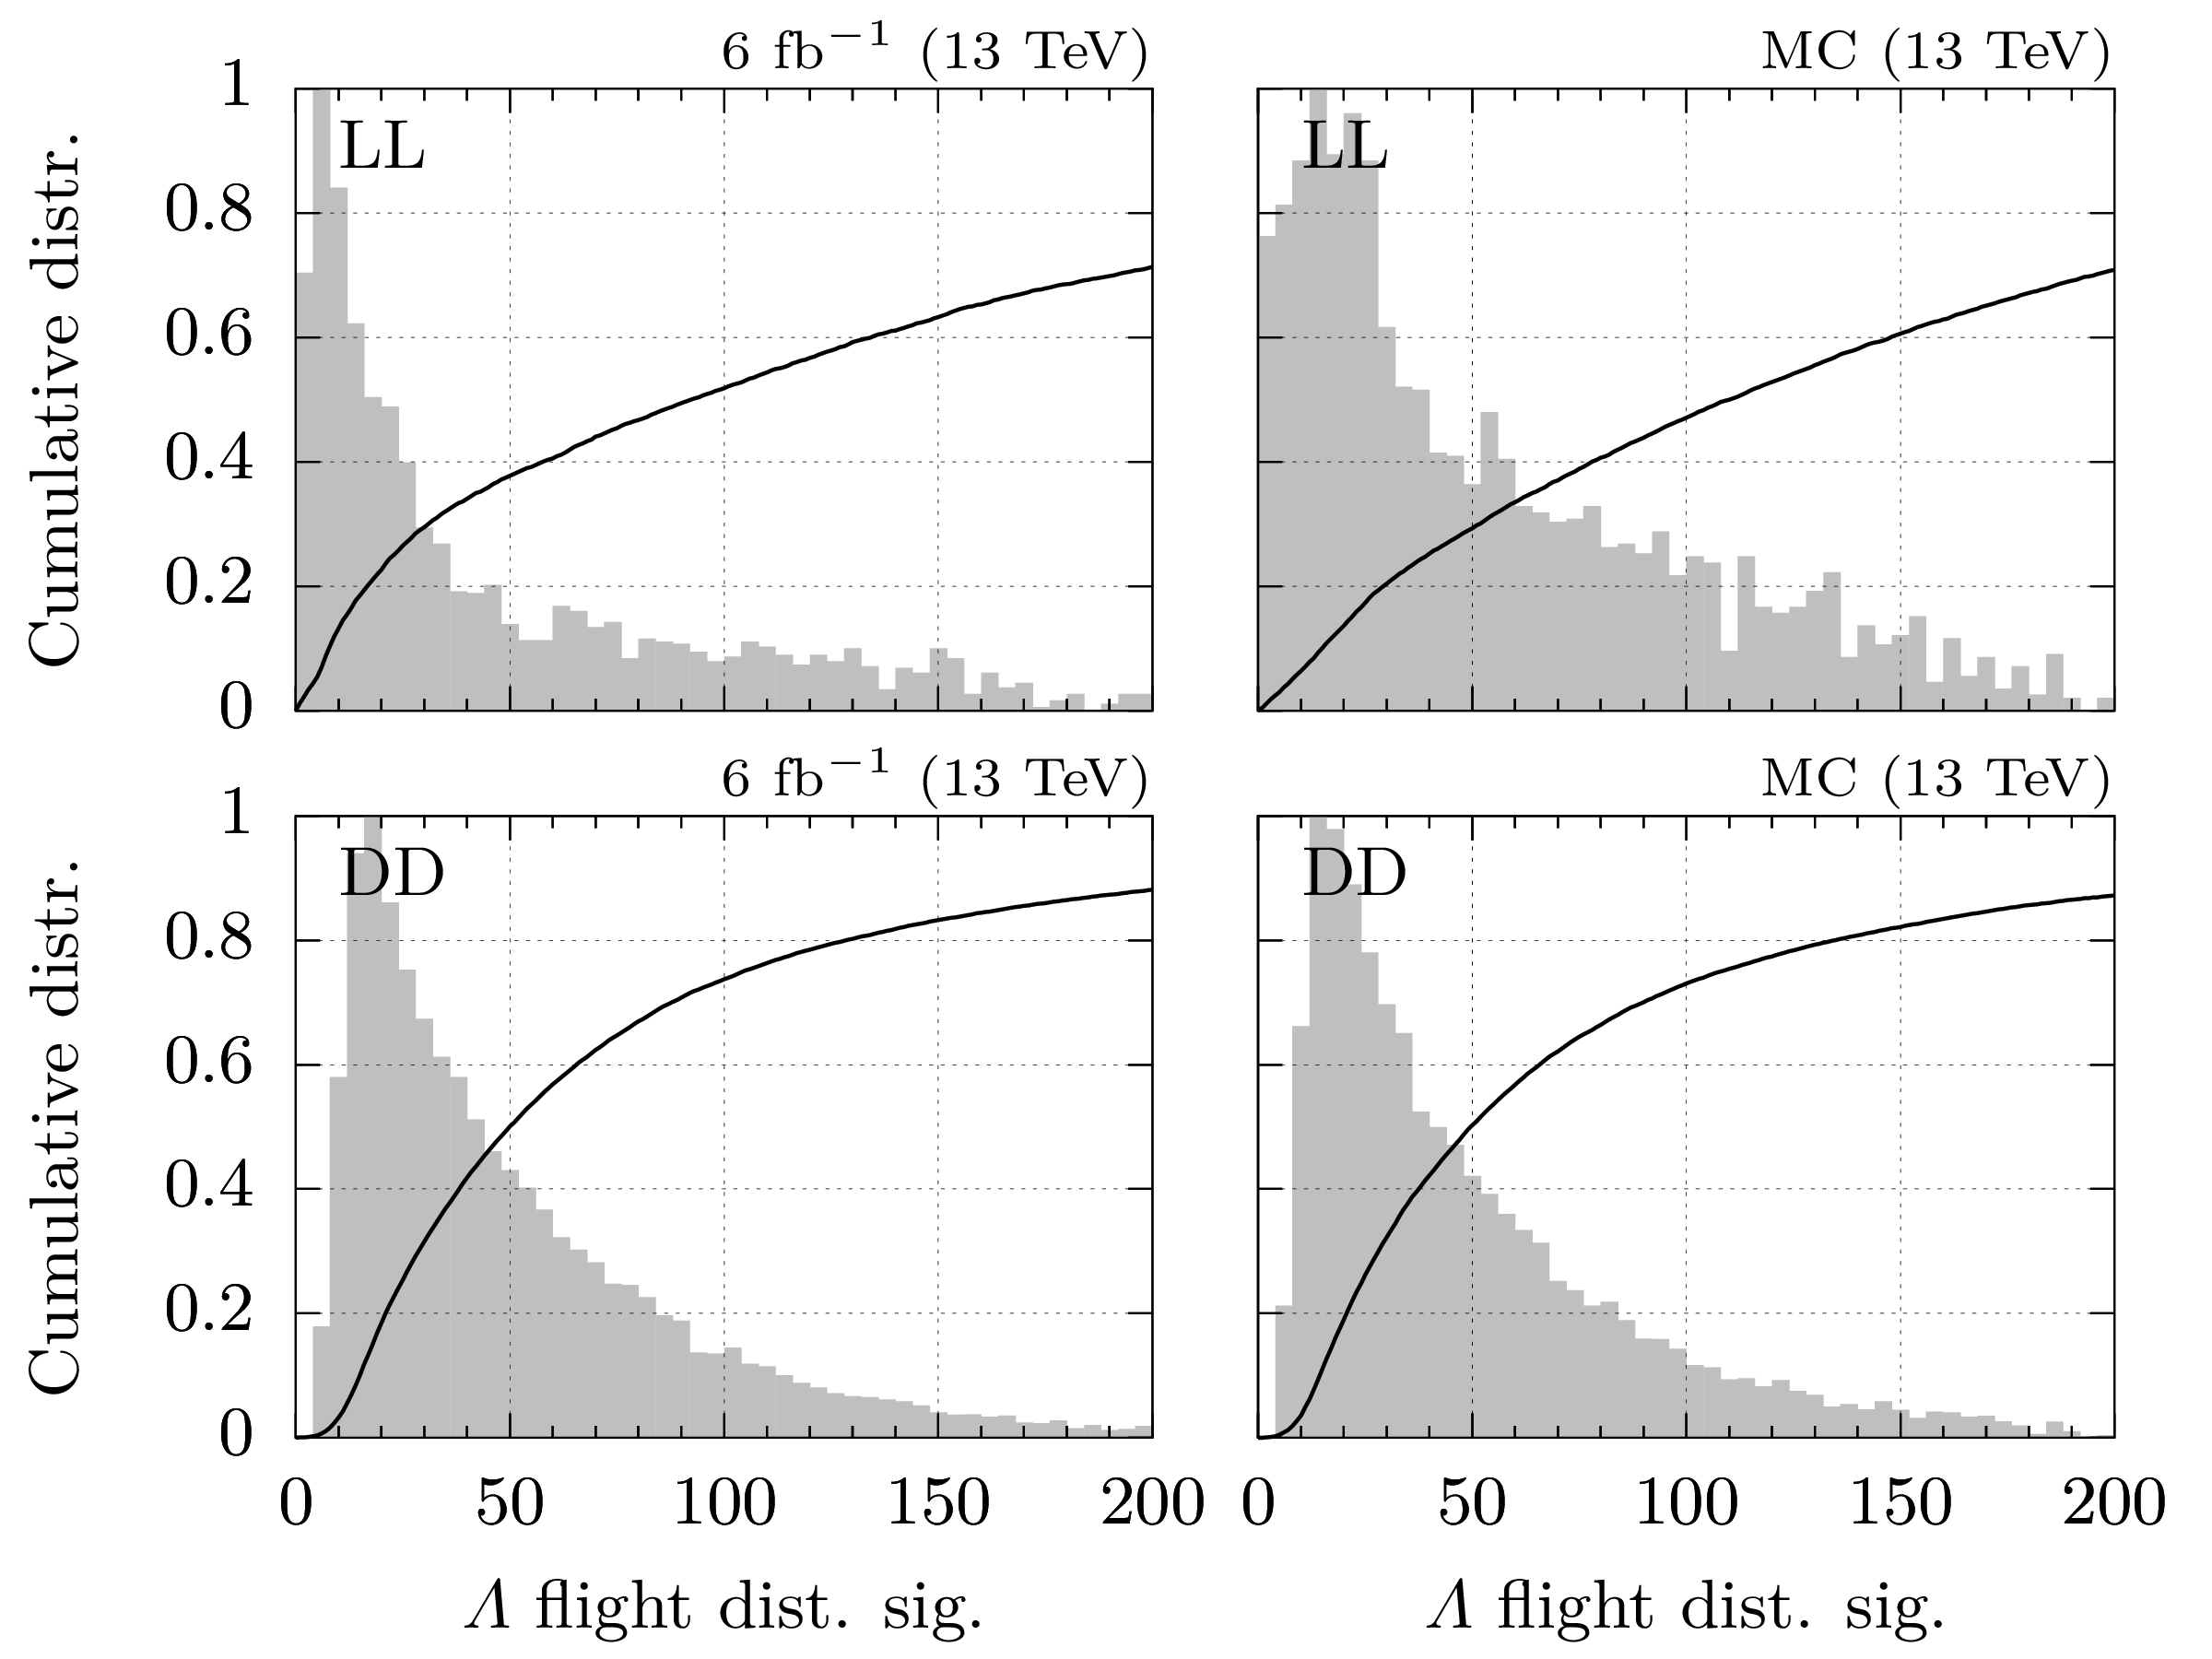
\includegraphics[scale=1.]{Lb2JpsiLz_weighting/LzFDs.png}
    \caption{Cumulative distribution (solid line) of the \Lz flight distance over the corresponding standard deviation for different track types (top and bottom), and for recorded data in the defined signal regions (left) and \gls{truthmatched} simulated events in the signal region (right). The gray shaded areas indicate the corresponding distributions of the respective significance of the flight distance itself.}
    \label{fig:LzFDs_LbToJpsiLz}
\end{figure}

The combinatorial background in $m(\jpsi\Lz)$ (rec.\ data) is sufficiently linear such that the \gls{fom} as defined in Eq.~\eqref{eq:fom_LbToJpsiLz} can be evaluated with a sideband-subtraction, \cf{}~Fig.~\ref{fig:LbToJpsiLz_weighting_fom}.
(Definition of the signal and background regions are given in Sec.~\ref{sec:LbToJpsiLz_loosesel}.) %and indicated in the invariant mass distribution $m(\jpsi\Lz)$ shown in Fig.~\ref{fig:mLbToJpsiLz_loosesel}.)
\begin{figure}[htbp]
    \centering
    \begin{subfigure}{\textwidth}
        \centering 
        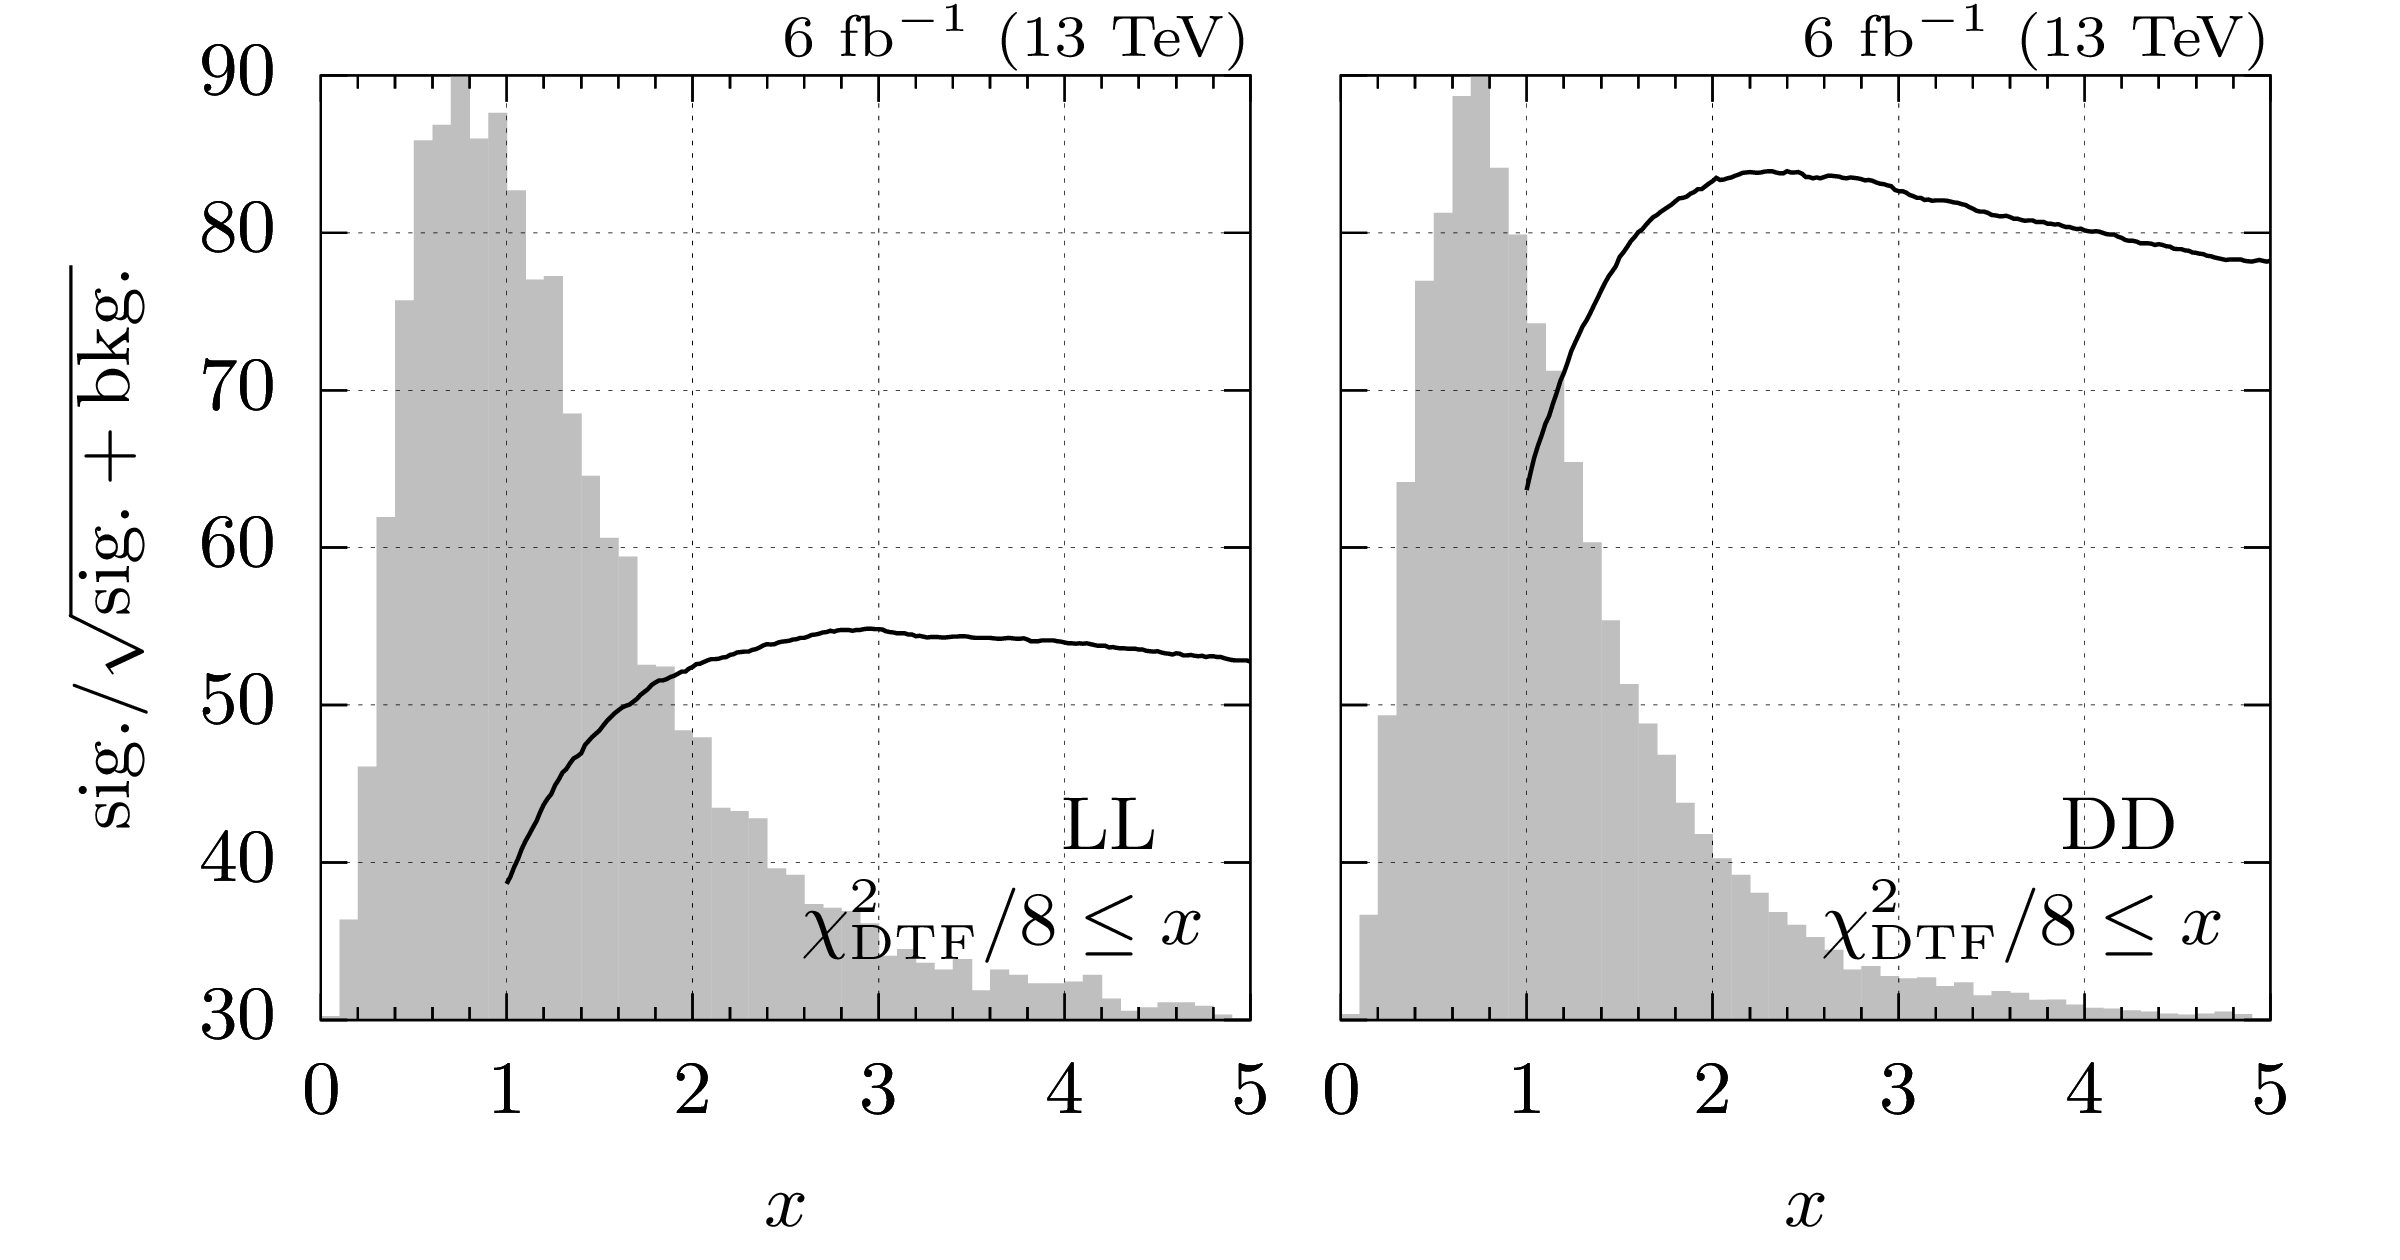
\includegraphics[scale=1.]{Lb2JpsiLz_weighting/sig_chi2.png}
        \caption{\Gls{fom} for veto events if $\chi^2_\text{DTF}/\mathrm{\gls{dof}} > x$.}
    \end{subfigure}
    \par\bigskip 
    \begin{subfigure}{\textwidth}
        \centering 
        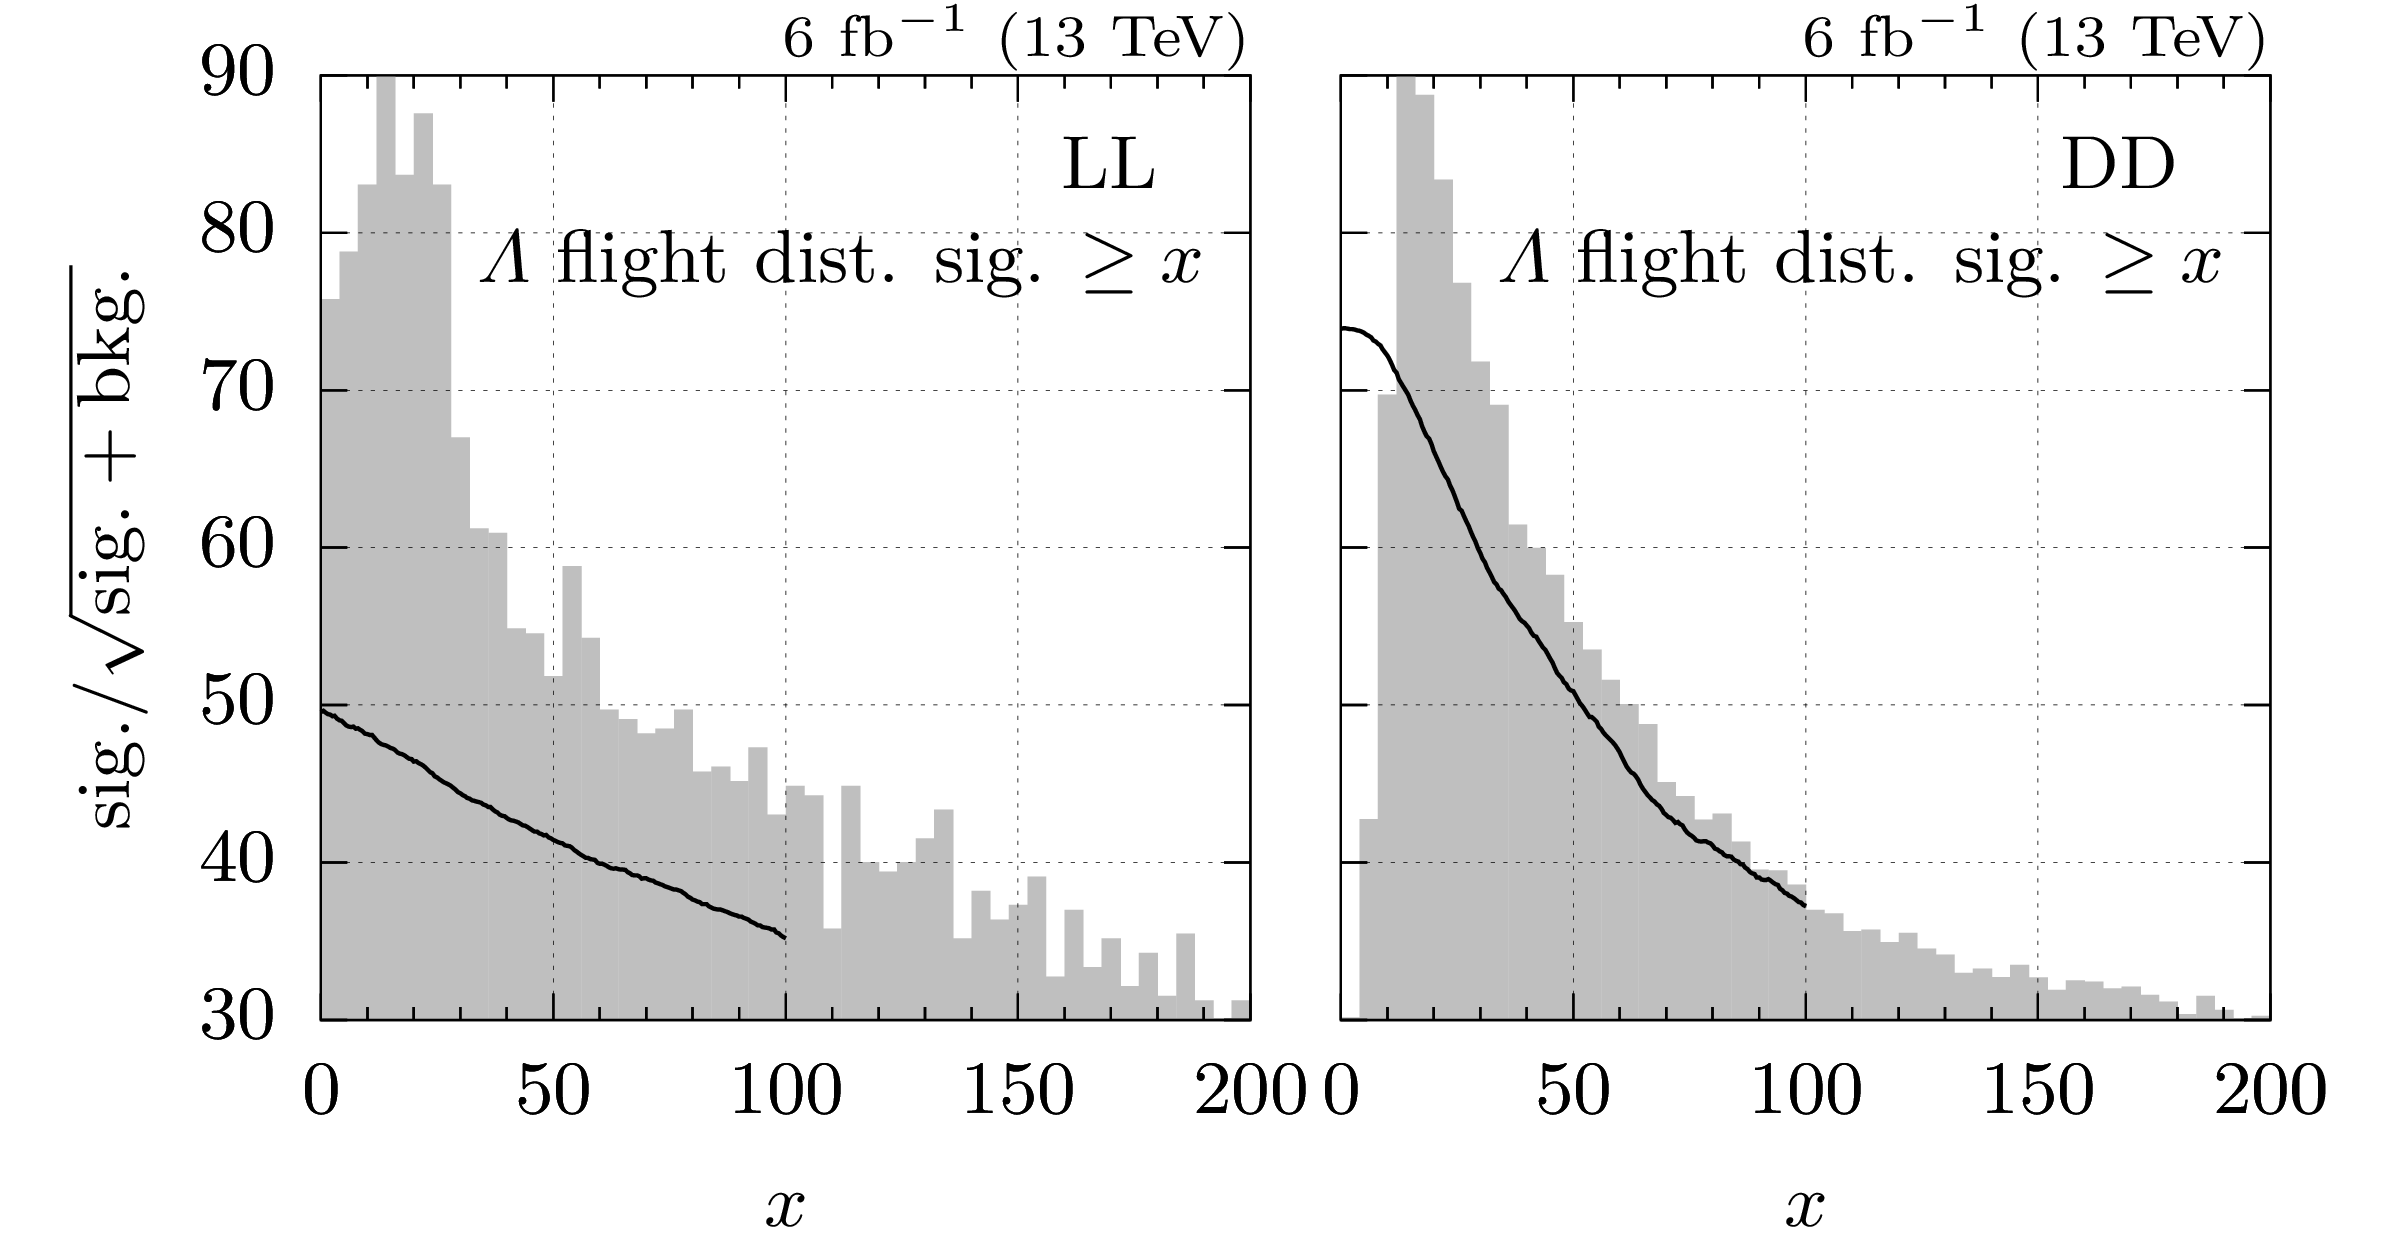
\includegraphics[scale=1.]{Lb2JpsiLz_weighting/sig_LzFDs.png}
        \caption{\Gls{fom} for veto events if \Lz flight distance significance $< x$.}
    \end{subfigure}
    \par\bigskip
    \begin{subfigure}{\textwidth}
        \centering 
        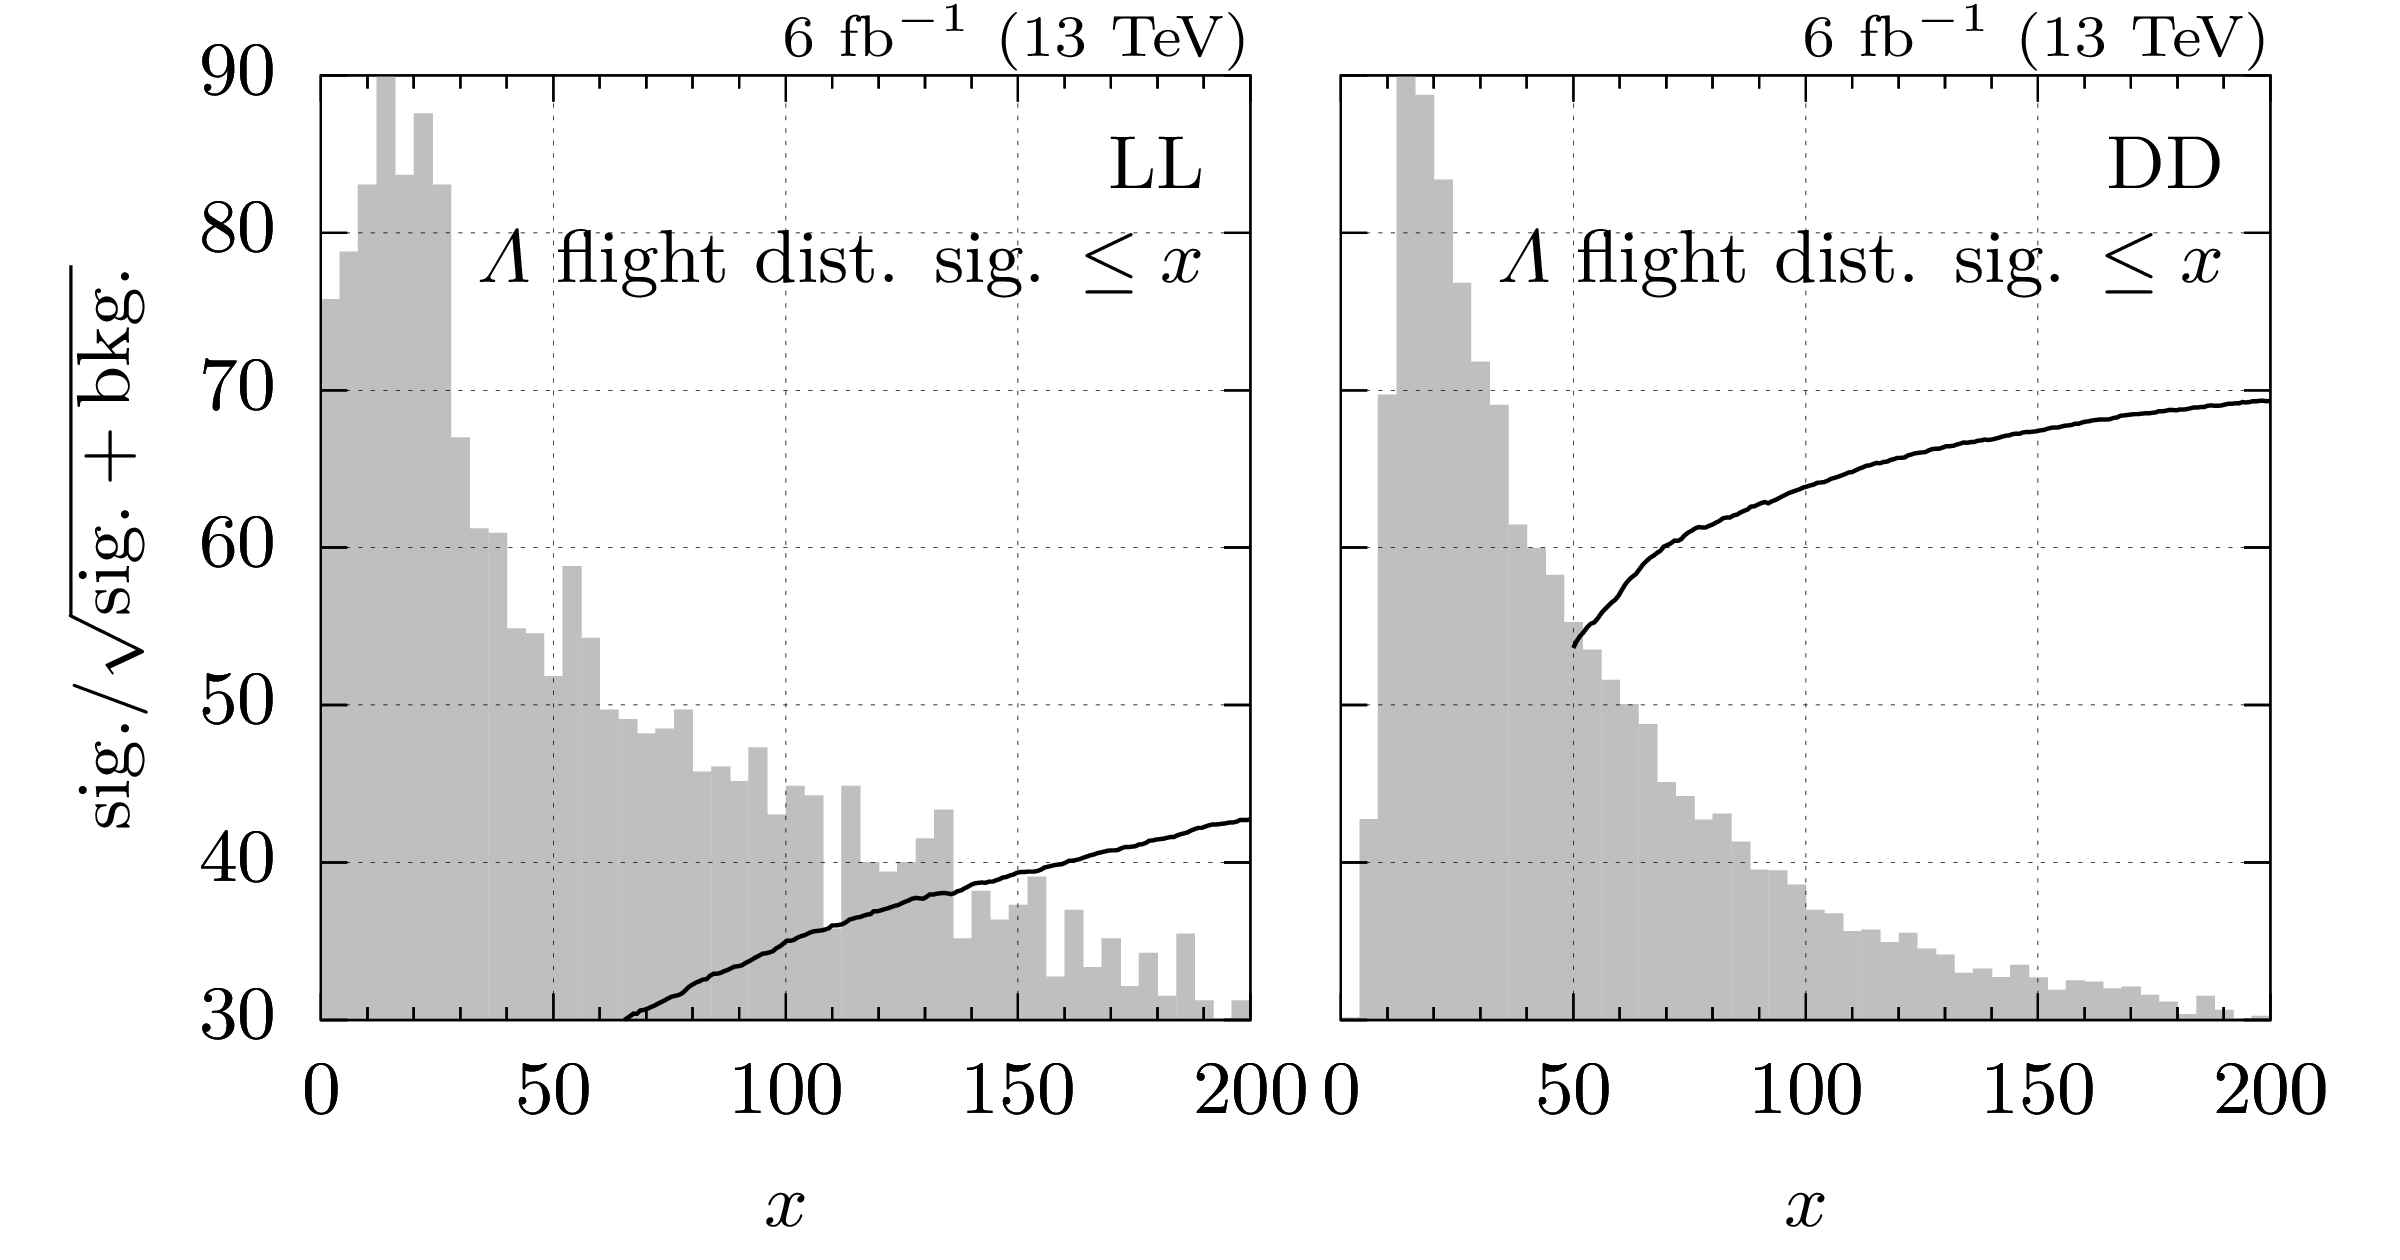
\includegraphics[scale=1.]{Lb2JpsiLz_weighting/isig_LzFDs.png}
        \caption{\Gls{fom} for veto events if \Lz flight distance significance $> x$.}
    \end{subfigure}
    \caption{\Gls{fom} defined as signal efficiency (solid black line) obtained by sideband-subtraction in recorded data and the corresponding distribution of \gls{truthmatched} simulated events (grey shaded area). The \gls{fom} of the \Lz flight distance significance is monotonic for requirements that either prefer large or low values and thus discourage an additional selection w.r.t.\ this feature.}
    \label{fig:LbToJpsiLz_weighting_fom}
\end{figure}
The signal significance for a selection w.r.t.\ $\chi^2_\text{DTF}$ has a maximum for \gls{LL} and \gls{DD} tracks, implying that signal events prefer smaller values of $\chi^2_\text{DTF}$, \ie{}, stronger support for the assumed hypothesis of the \gls{dtf}, and thus motivates the selection criterion for the tight selection
\begin{equation}
    \label{eq:LbToJpsiLz_tightsel}
    \chi^2_\text{DTF} \overset{!}{\le}
    \begin{cases}
        3 & \text{(LL)}, \\
        2 & \text{(DD)},
    \end{cases}
\end{equation}
whereas the \gls{fom} of the \Lz flight distance significance is monotonic for requirements that either prefer large or low values and thus discourage an additional selection w.r.t.\ this feature.
In Fig.~\ref{fig:mLbToJpsiLz_tightsel} we show the invariant mass $m(\jpsi\Lz)$ after applying this and all previously mentioned selection requirements.

\begin{figure}[htbp]
    \centering
    \begin{subfigure}[b]{.49\textwidth}
        \centering
        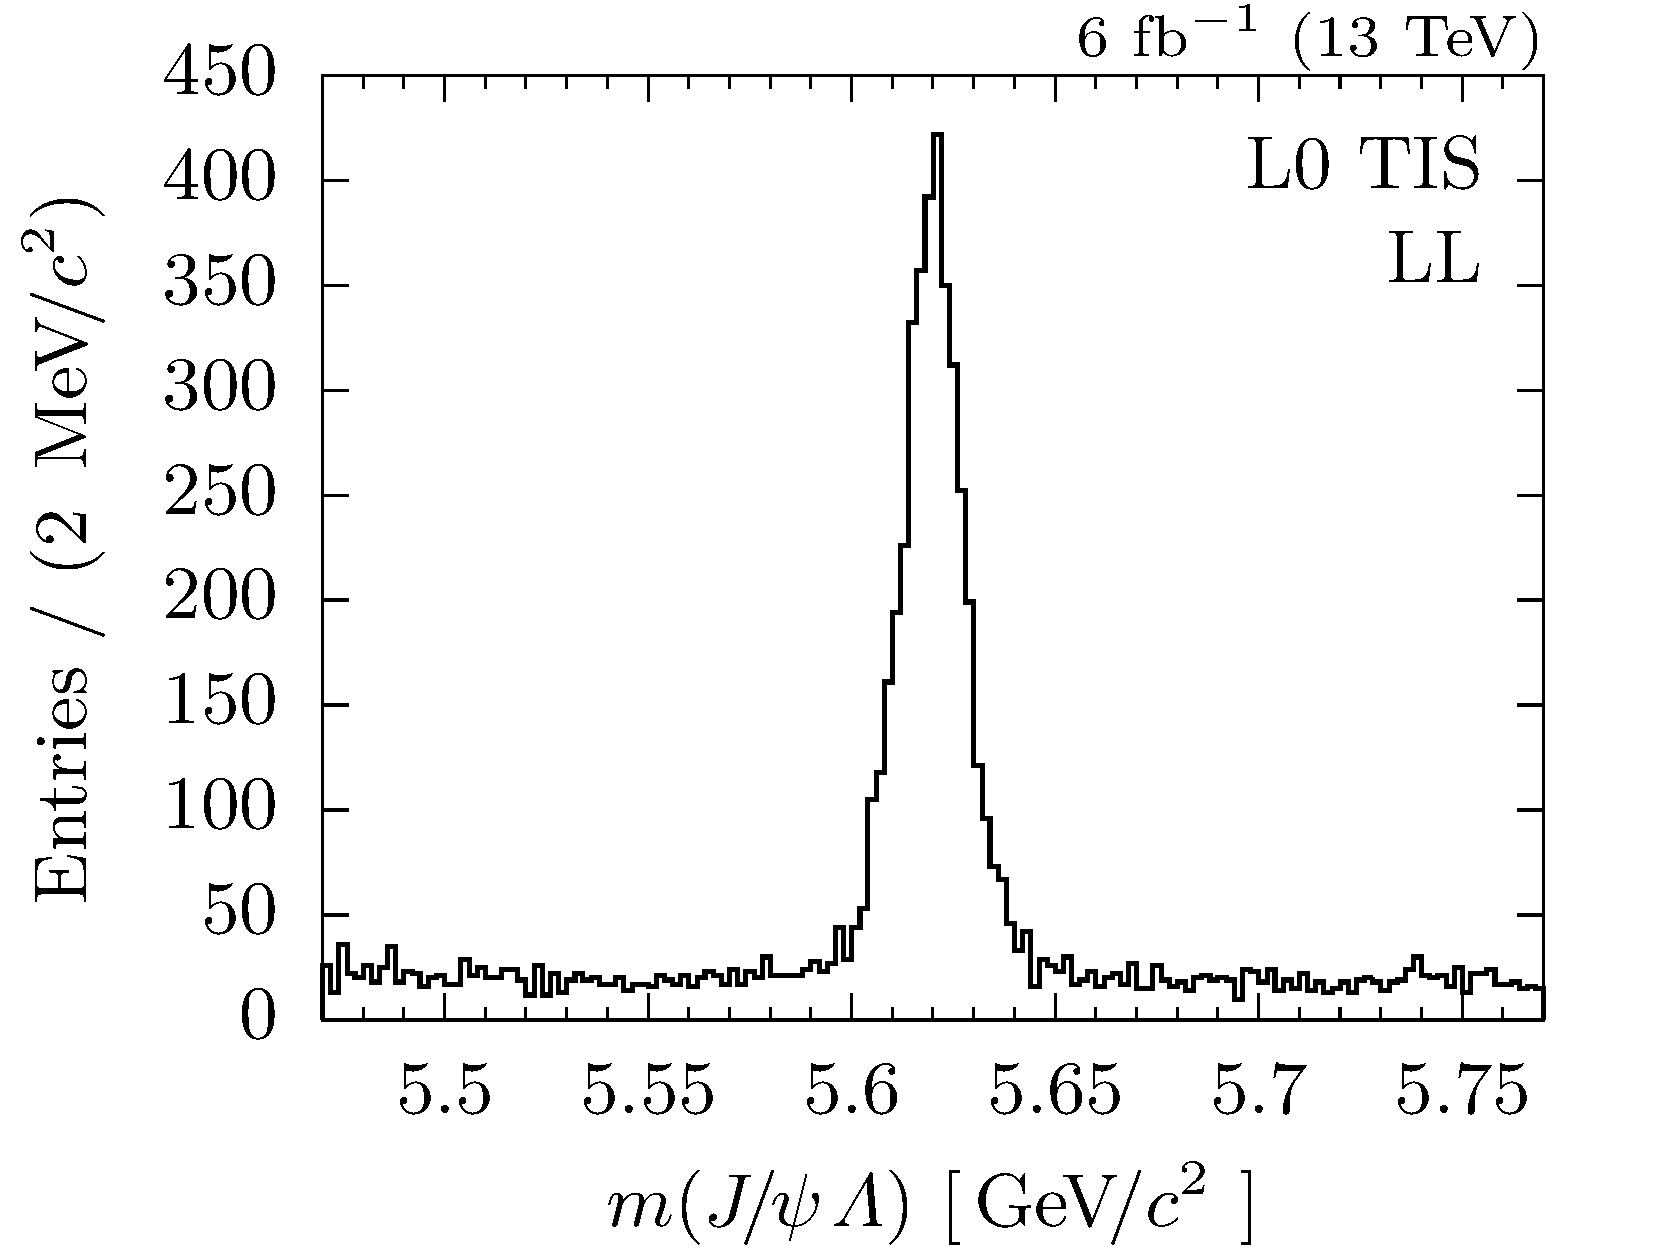
\includegraphics[scale=1.]{Lb2JpsiLz_weighting/hLbM_LL_final.png}
        \caption{\Lz candidates rec.\ from \gls{LL} tracks.}
    \end{subfigure}
    \begin{subfigure}[b]{.49\textwidth}
        \centering
        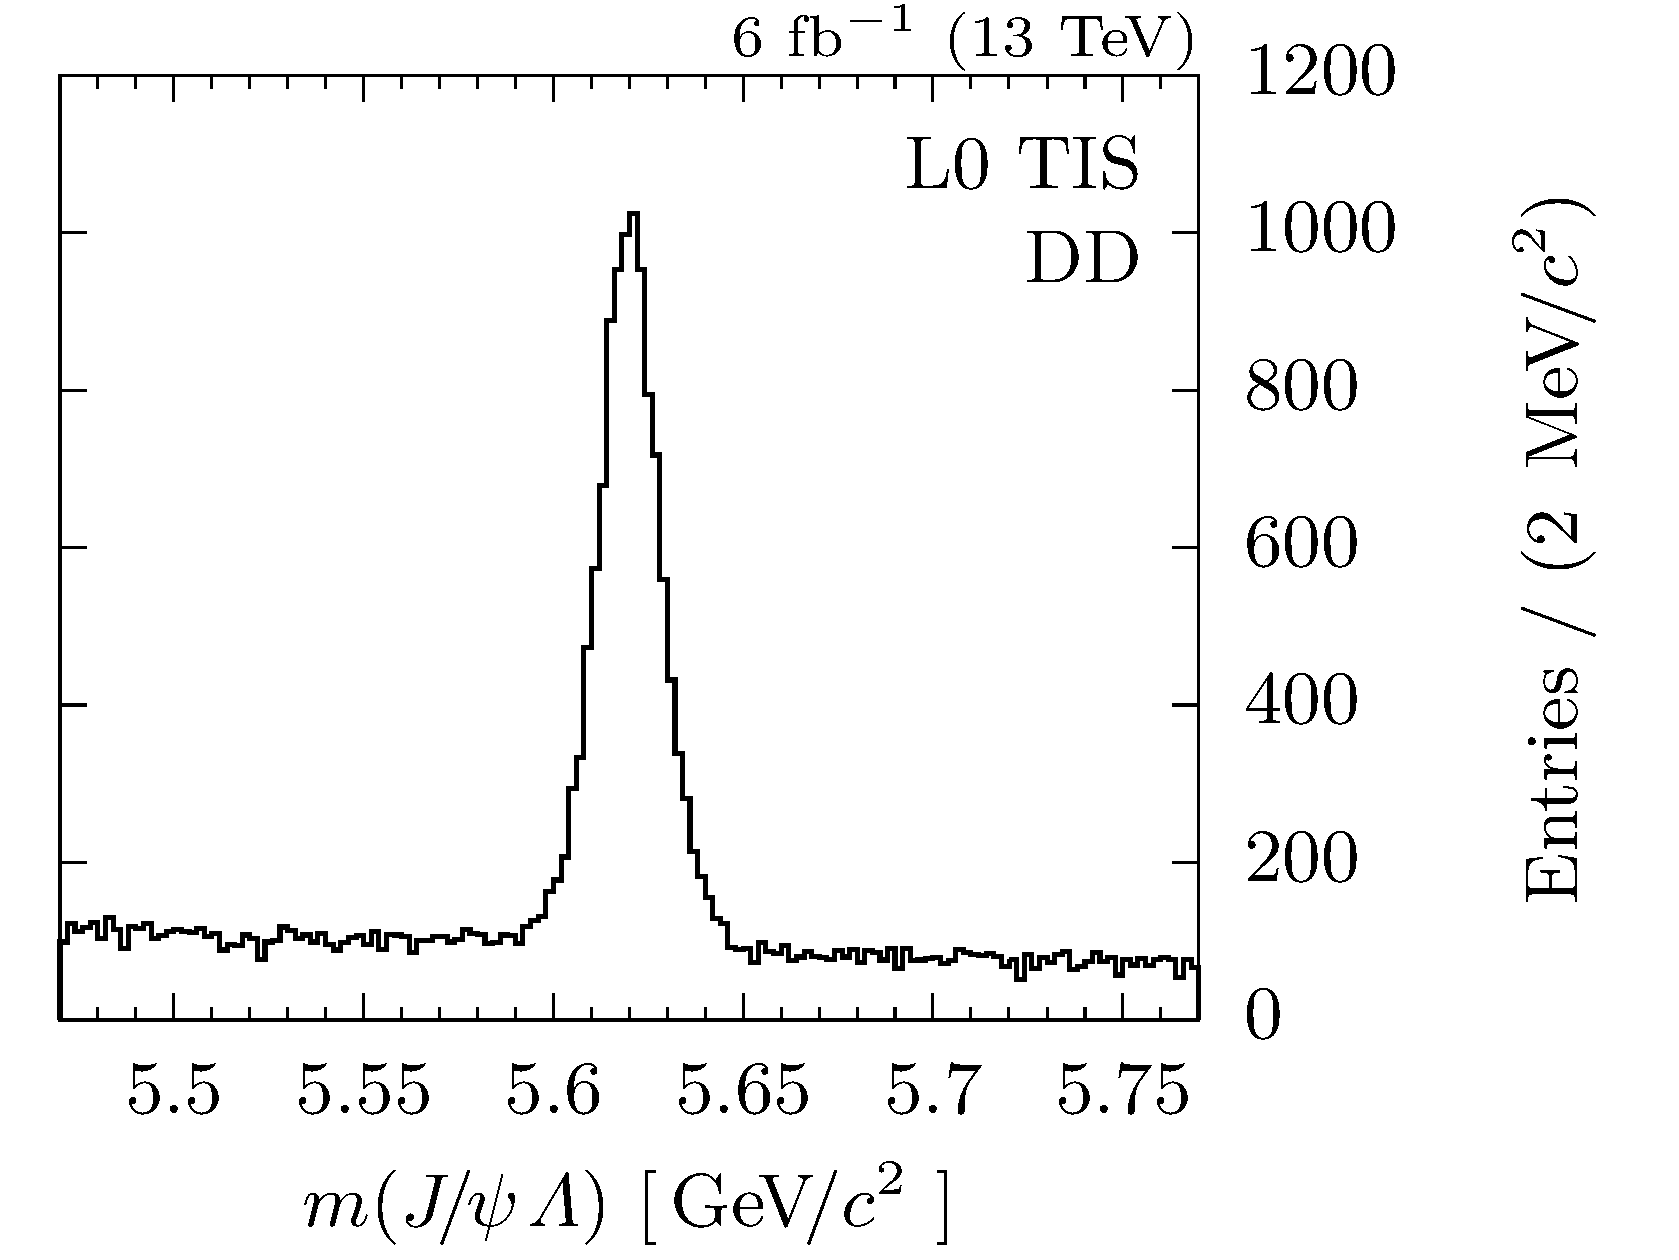
\includegraphics[scale=1.]{Lb2JpsiLz_weighting/hLbM_DD_final.png}
        \caption{\Lz candidates rec.\ from \gls{DD} tracks.}
    \end{subfigure}
    \caption{Combined invariant mass of \jpsi and \Lz candidates after tight selection from recorded data. (Including \gls{lzero} \gls{tis} only requirement.) This selection is used for determining the weights for tuning \gls{mc} simulated \Lb decays.}
    \label{fig:mLbToJpsiLz_tightsel}
\end{figure}

\subsubsection{Efficiency Determination of the Tight Selection}
\label{sec:weights_tightsel}
The technique of sideband subtraction also leverages the estimation of a data driven efficiency determination of the selections given in Eq.~\eqref{eq:LbToJpsiLz_tightsel} by evaluating
\begin{equation*}
    \varepsilon := \frac{n_\text{sig}}{n_\text{sig} + \bar n_\text{sig}} \,,
\end{equation*}
where $n_\text{sig}$ and $\bar n_\text{sig}$ are the amount of signal events that pass the selection and the amount of events that are rejected, respectively.
The uncertainty $u_\varepsilon$ of each of these figures is given by the uncertainty of the mean background ($f \sqrt{n_\text{sideband}} = \sqrt{f n_\text{bkg}}$), the fluctuation of the true background around the mean background in the signal region ($\sqrt{n_\text{bkg}}$) and the fluctuation of the true signal around the mean signal ($\sqrt{n_\text{sig}}$)
\begin{equation*}
    u_\varepsilon = \sqrt{n_\text{sig} + (1 + f) n_\text{bkg}}\,,
\end{equation*}
where $f$ is the scale factor that translates the number of observed background events in the sideband region $n_\text{sideband}$ to the estimated number of background events in the signal region $n_\text{bkg} = f \times n_\text{sideband}$.
The amounts $n_\text{sig}$ and $\bar n_\text{sig}$ are statistically independent, hence the uncertainty of the cut efficiency $\varepsilon$ can be extracted by ordinary error propagation.
In Tab.~\ref{tab:LbToJpsiLz_tighsel_eff} we show $n_\text{sig}$ with its associated uncertainty $\sqrt{(1 + f) n_\text{bkg}}$, as well as the selection efficiencies~$\varepsilon$.

\begin{table}[htbp]
    \centering
    \caption{Total amount of signal events $n_\text{sig}$ after applying the tight selection to recorded \decay{\Lb}{\jpsi\Lz} data, as well as the respective selection efficiency $\varepsilon$.}
    \label{tab:LbToJpsiLz_tighsel_eff}
    \begin{tabular}{ccc}
        \toprule
        & $n_\text{sig}$ & $\varepsilon$ \\
        \midrule
        \gls{LL} & $\num{3653} \pm 33$ & $(91.4 \pm 1.2) \,\%$ \\
        \gls{DD} & $\num{9590} \pm 70$ & $(79.1 \pm 0.9) \,\%$ \\
        \bottomrule
    \end{tabular}
\end{table}

\section{Extraction of Weights}
The features transverse momentum $\pt(\Lb)$ and pseudorapidity $\eta(\Lb)$ of the \Lb are not uncorrelated, but related via the identity relation
\begin{equation*}
    \eta = \operatorname{artanh} \frac{p_z}{p} = \operatorname{artanh} \sqrt{1 - \left( \frac{\pt}{p} \right)^2} \,,
\end{equation*}
where $\operatorname{artanh}$ is the inverse hyperbolic tangent (aka area hyperbolic tangent), and $p_z$ and $p$ the $z$-component and magnitude of the momentum, respectively.

%\begin{figure}[htbp]
%    \centering
%    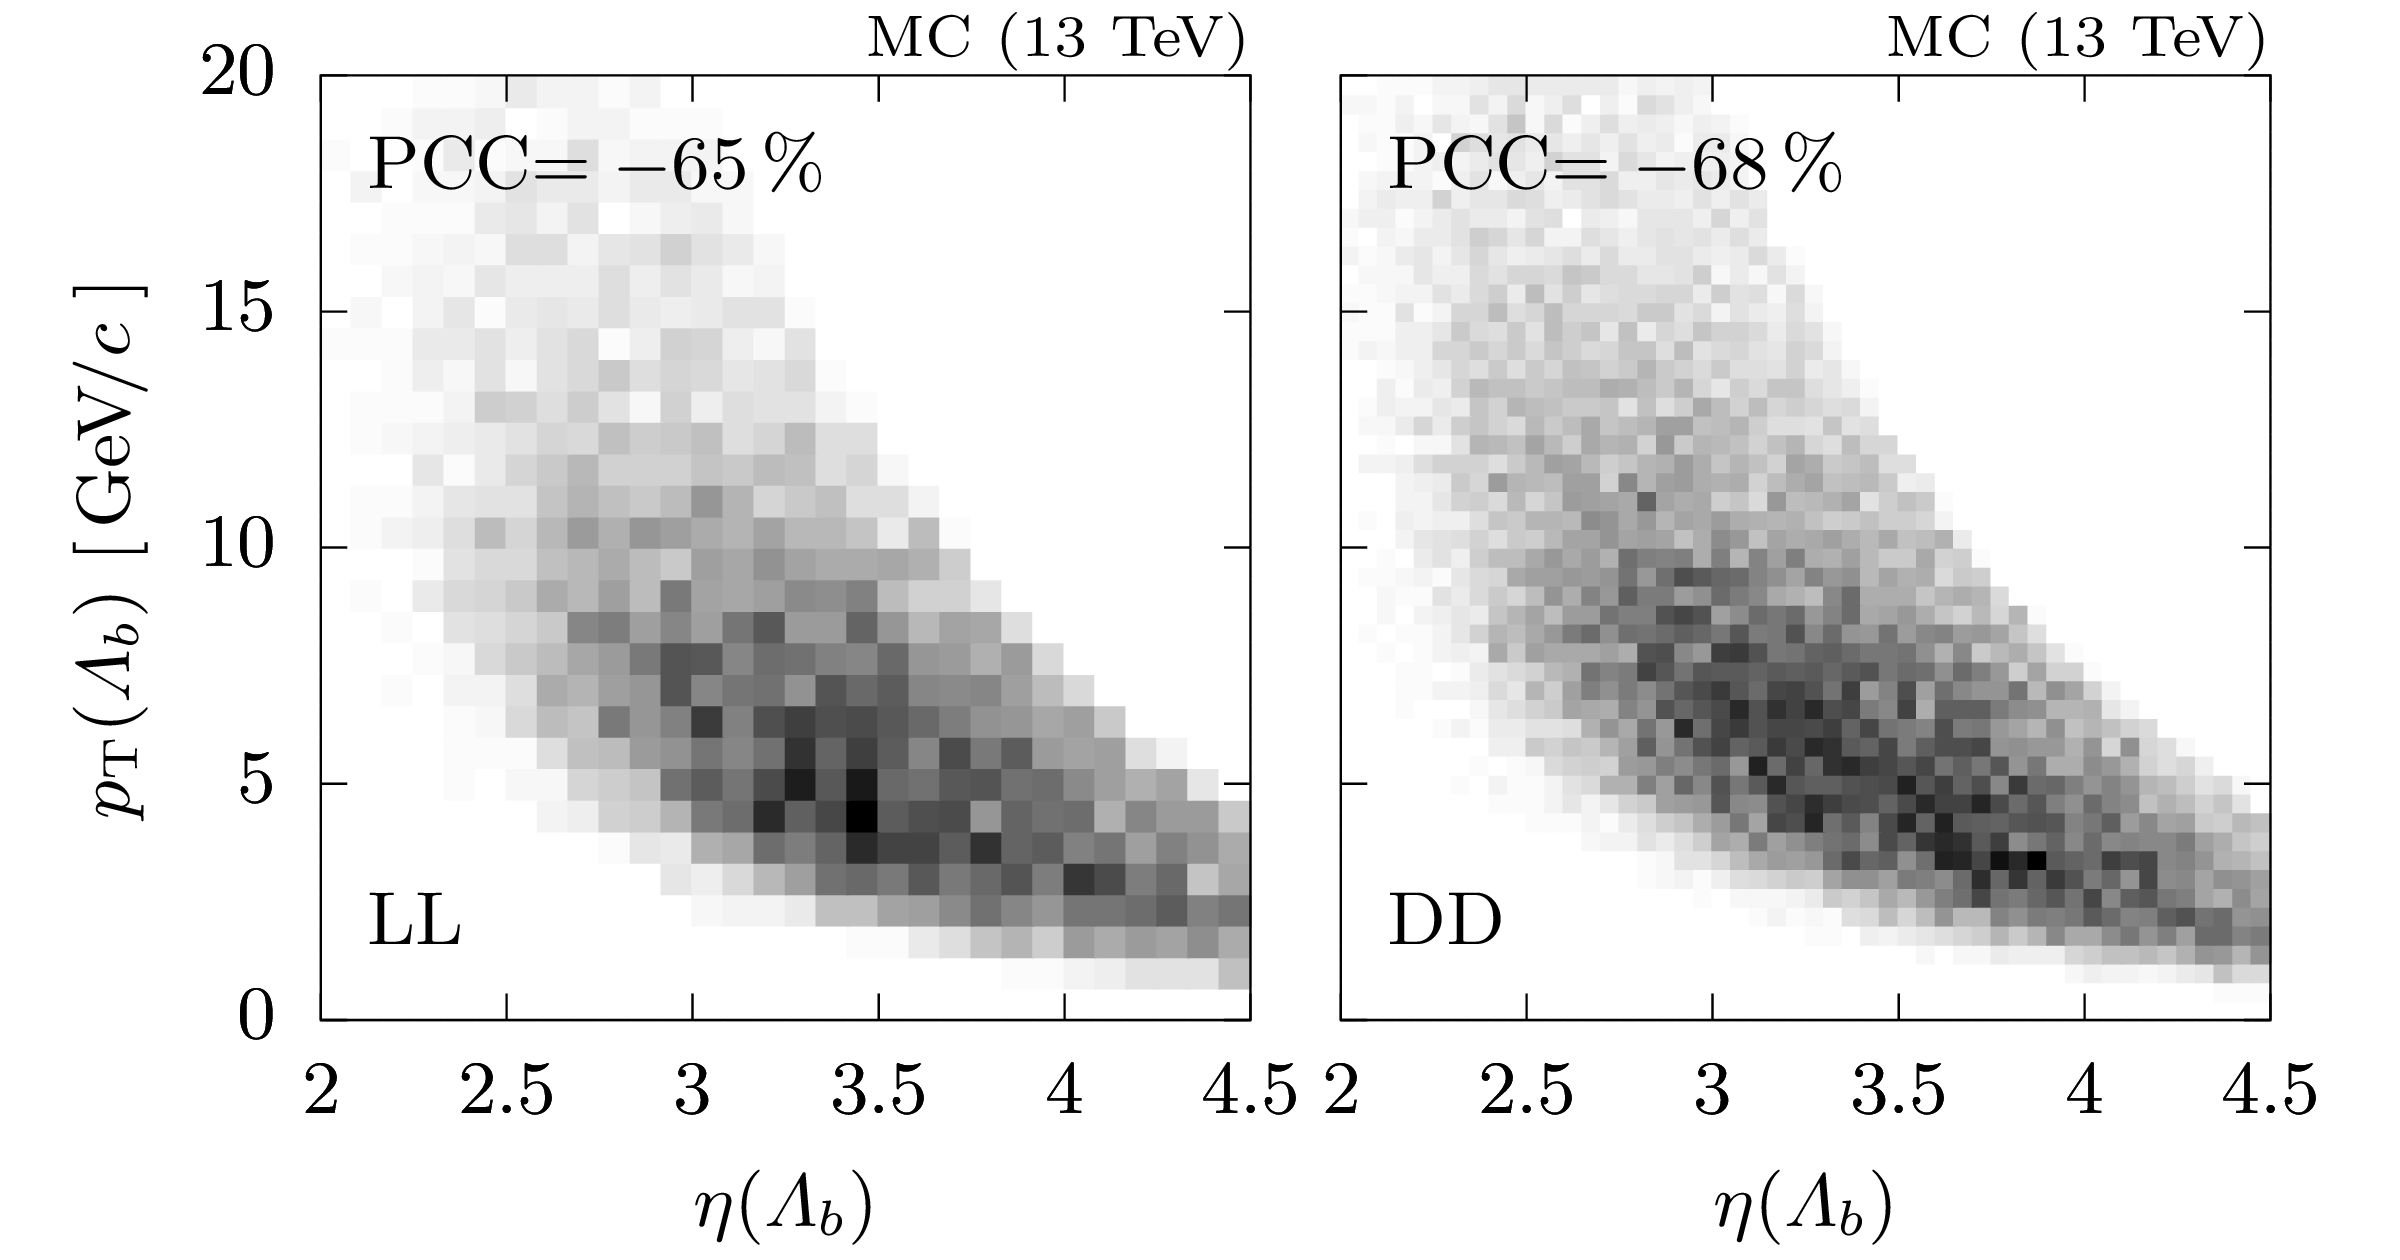
\includegraphics[scale=1.]{Lb2JpsiLz_weighting/corr_eta_pT.png}
%    \caption{Correlation between $\pt(\Lb)$ and $\eta(\Lb)$, as well as the corresponding \gls{pcc} values for \gls{LL} (left) and \gls{DD} tracks (right), estimated for \gls{truthmatched} MC simulated \decay{\Lb}{\jpsi\Lz} events.}
%    \label{fig:corr_eta_pT_LbToJpsiLz}
%\end{figure}
%
%In Fig.~\ref{fig:corr_eta_pT_LbToJpsiLz} we show the correlation between $\pt(\Lb)$ and $\eta(\Lb)$, as well as the corresponding \gls{pcc} values for \gls{LL} (left) and \gls{DD} tracks (right), estimated for \gls{truthmatched} MC simulated \decay{\Lb}{\jpsi\Lz} events.
%The correlation is approximately $-65\,\%$ and $-68\,\%$ for \gls{LL} and \gls{DD} tracks, respectively.
Due to this non-negligible correlation, altering one distribution will also affect the other and vice versa.
Ideally, the extraction of weight factors should be performed in the 2d-plane of both variables.
Reliable weights, though, also require decent statistics which turned out to be problematic, especially for \gls{LL} tracks.

We try two different schemes for extracting weights.
First, we only consider the respective marginal distributions and find the weights in an iterative approach.
The underlying assumption is a factorization of the weights in the 2d-plane $w(\pt, \eta) = w_1(\pt) \times w_2(\eta)$ and thus, per definition, ignores all correlation contributions.
We cross-check this assumption with a third quantity $p(\Lb)$ which is another marginal distribution in the $\pt$-$\eta$ space.

In this first scheme we discover unexpected deviations between the distributions of $\eta(\Lb)$ for different track types but at the same time a decent compatibility with one for all $\eta(\Lb)$ weights w.r.t.\ the given statistical uncertainties.
This motivates our second scheme where weights are extracted based on $\pt(\Lb)$ only.

\subsection{Truth Matched vs. Sideband Subtracted MC Simulated Events}
\label{sec:LbToJpsiLz_tm_vs_ss}

Similar to recorded data, \gls{mc} simulated events contain not only signal, but also background events coming either from true physical background processes or are combinatoric remnants.
A marked difference between recorded and simulated events is that the latter could be attached with a label and thus, in theory, can be unambiguously identified as signal (\gls{truthmatched}) or background event (\textit{unmatched}).
However, in practice this approach suffers from a non-zero mistag probability during reconstruction which introduces an unphysical error.
This error has no counter part in recorded data which is critical when correlated with the variables that are the objective of the weighting scheme.

\begin{figure}[htbp]
    \centering
    \begin{subfigure}{\textwidth}
        \centering
        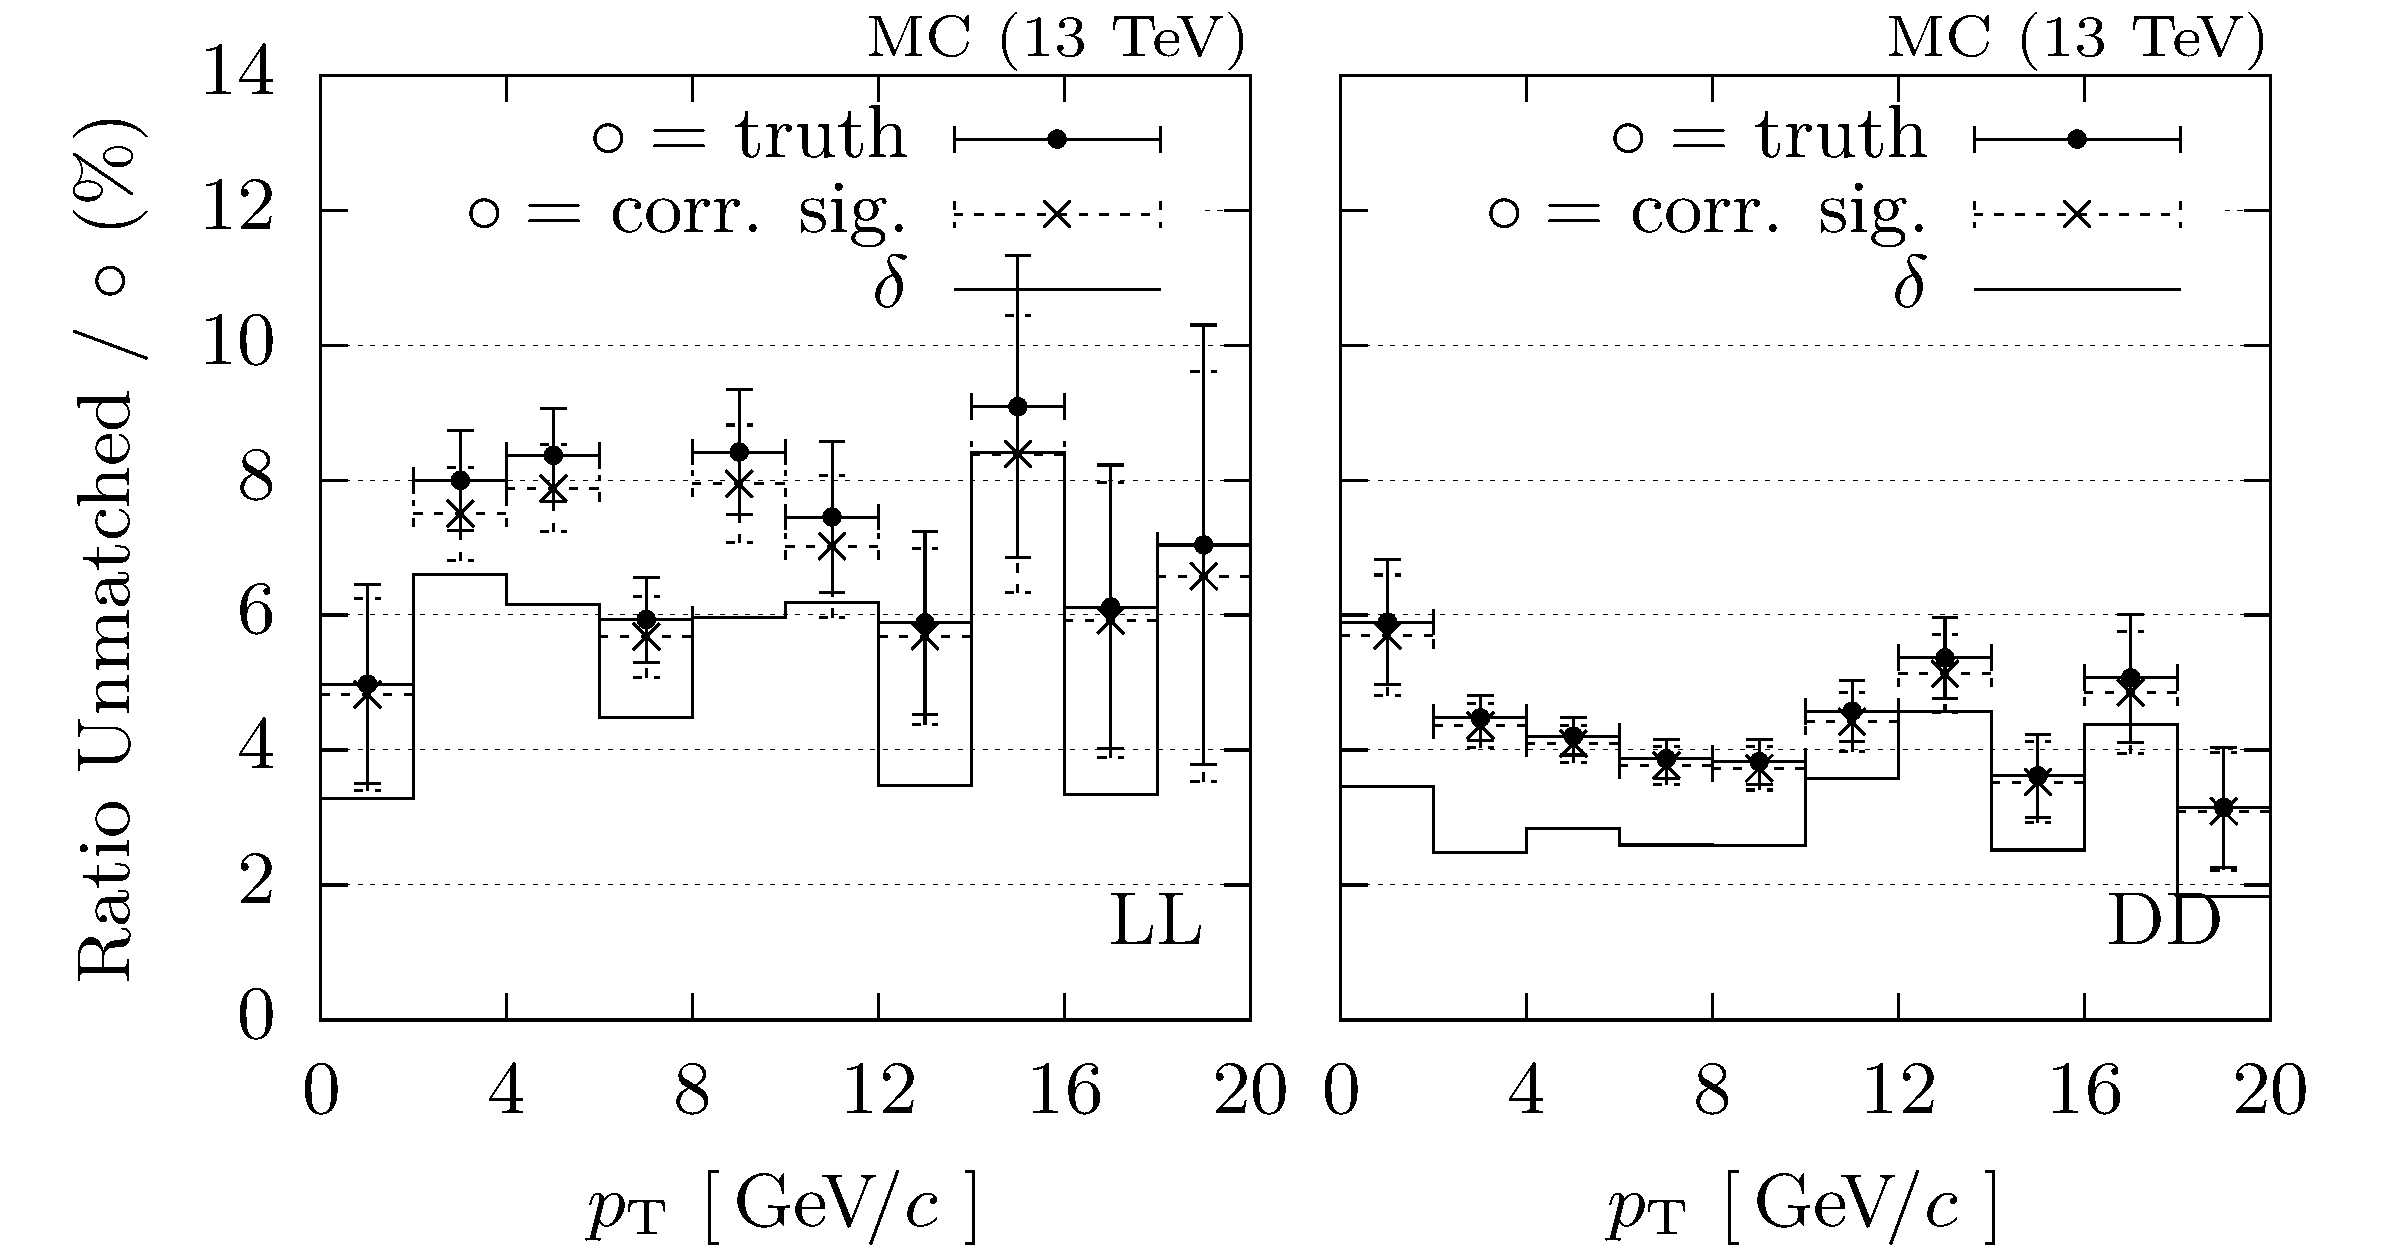
\includegraphics[scale=1.]{Lb2JpsiLz_weighting/htmratio_pT.png}
    \end{subfigure}
    \par\bigskip 
    \begin{subfigure}{\textwidth}
        \centering
        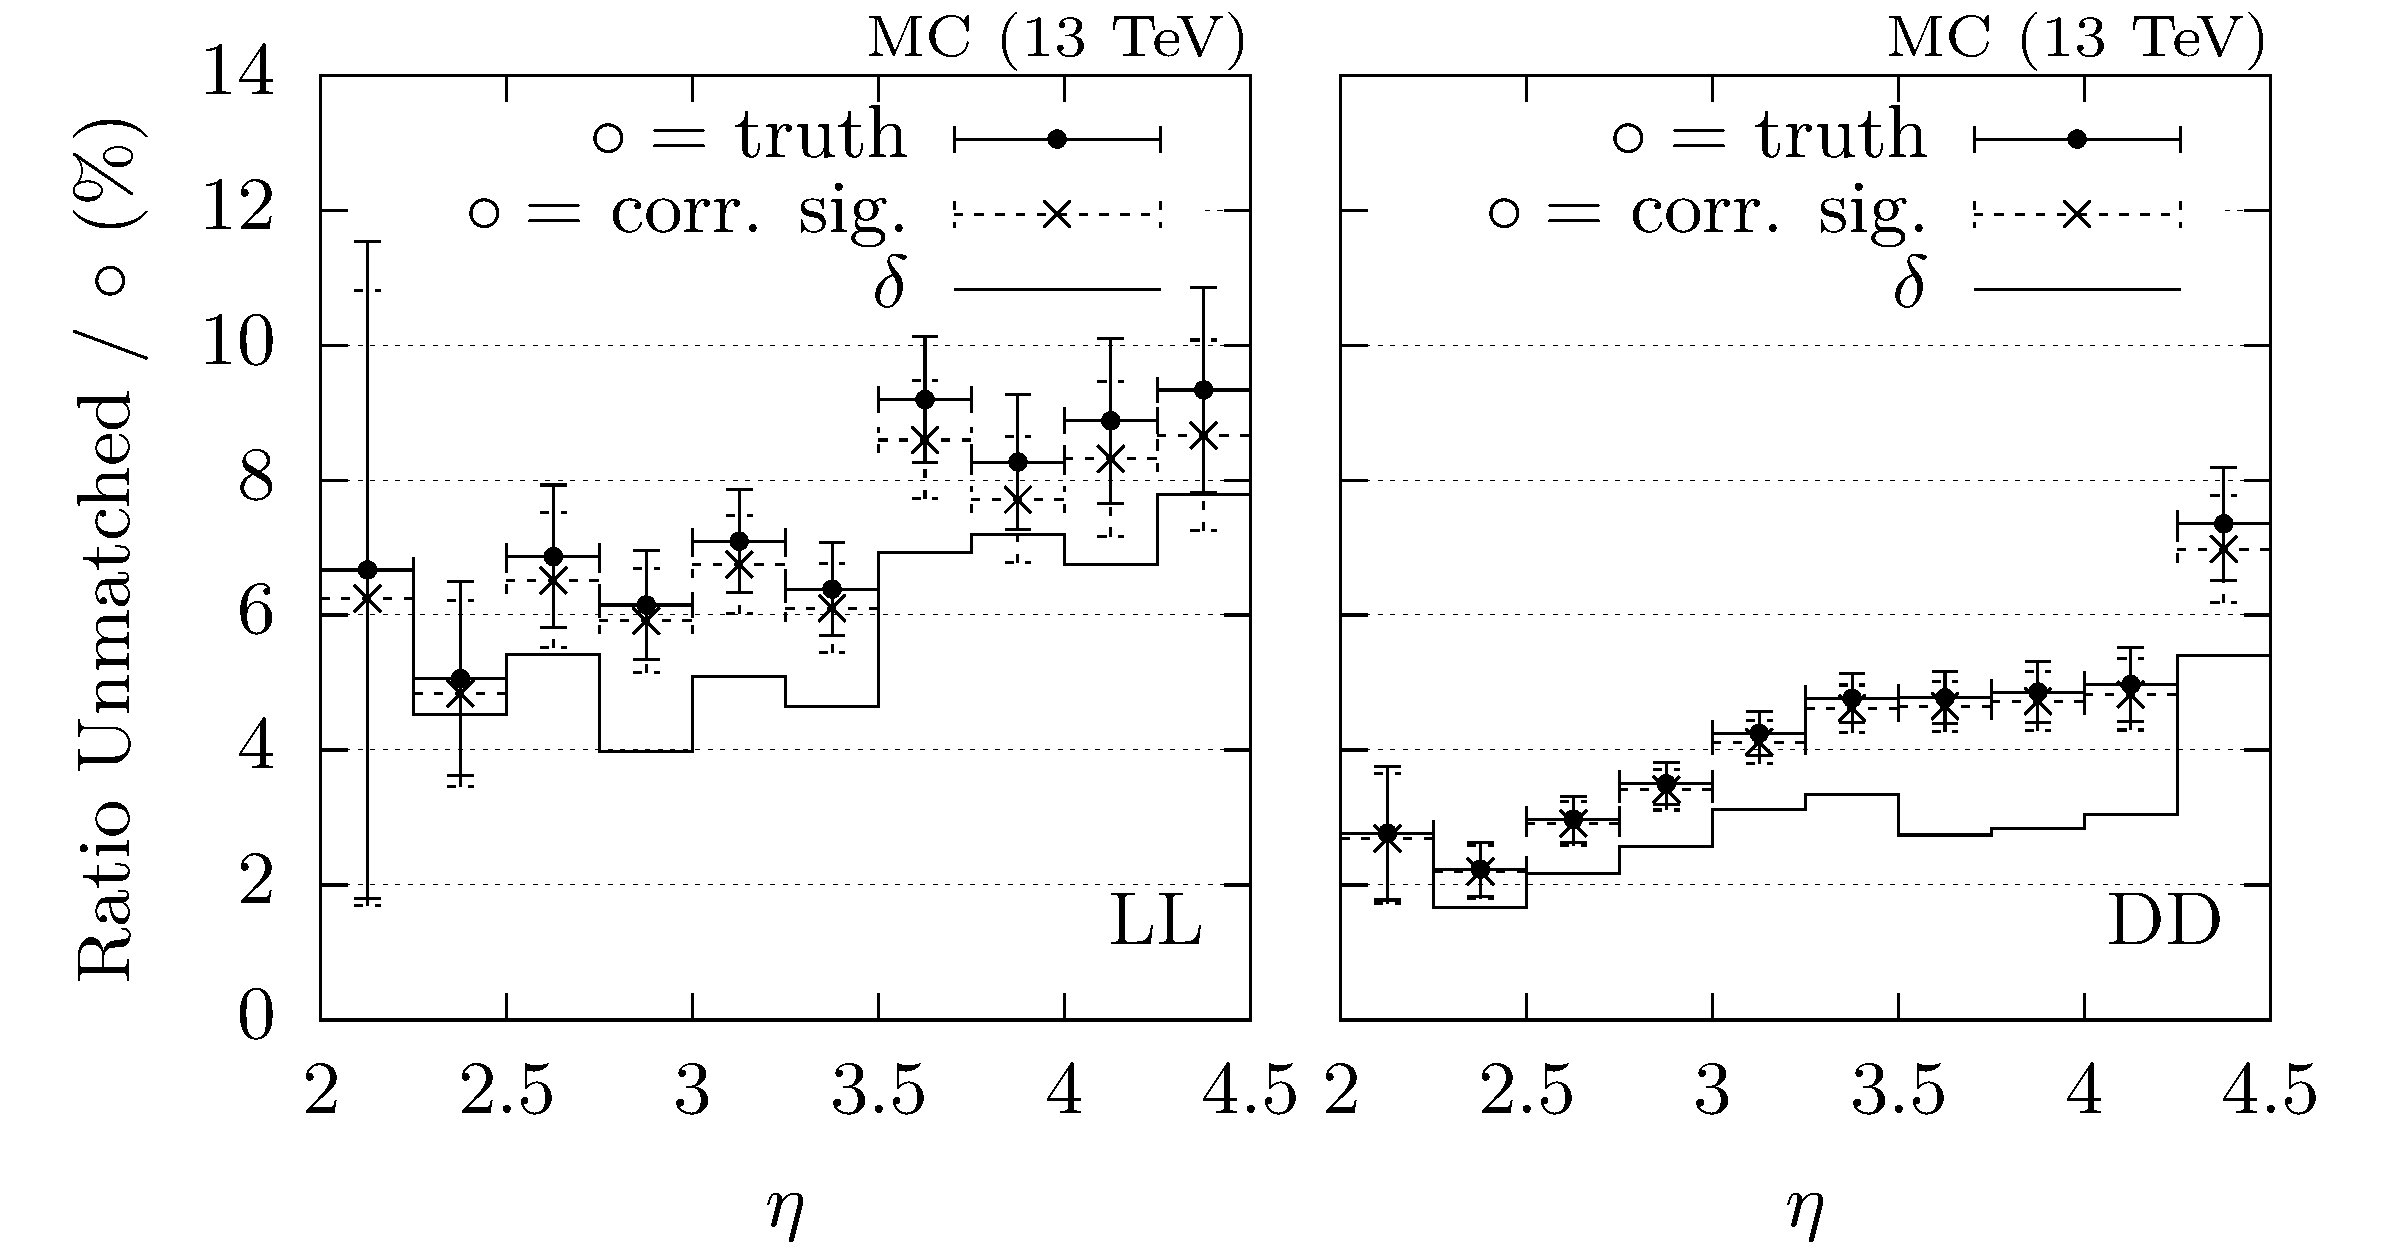
\includegraphics[scale=1.]{Lb2JpsiLz_weighting/htmratio_eta.png}
    \end{subfigure}
    \caption{Comparison of the ratio of unmatched and \gls{truthmatched} (referred to as \textit{truth}) with the ratio of unmatched and sideband corrected events (referred to as \textit{corr. sig.}) in bins of $\pt(\Lb)$ (top) and $\eta(\Lb)$ (bottom) for track types \gls{LL} (left) and \gls{DD} (right). The values of $\delta$, as defined in Eq.~\eqref{eq:weightdelta}, are shown at the same $y$-axis. The given error bars do not account for the strong correlations between unmatched and \gls{truthmatched} events.}
    \label{fig:htmratio_LbToJpsiLz}
\end{figure}

In the Fig.~\ref{fig:htmratio_LbToJpsiLz} we compare the ratio of unmatched and \gls{truthmatched} events with the ratio of unmatched and sideband corrected events as a function of $\pt(\Lb)$ and $\eta(\Lb)$.
The samples used for determining the ratios are pairwise uncorrelated, whereas the ratios themselves are strongly correlated which has to be taken into account when comparing the distribution of the ratios.
We define $\delta$ as the correction when using \gls{truthmatched} events during the weighting procedure instead of sideband corrected simulated events,
\begin{equation}
    \label{eq:weightdelta}
    1 + \delta := \frac{b'}{b} = 1 + \frac{\Delta}{a/b'} \,,
\end{equation}
where $a$, $b$ and $b'$ are the amount of unmatched, \gls{truthmatched} and sideband corrected simulated events, respectively and $\Delta$ is defined as the difference
\begin{equation*}
    \Delta := \frac{a}{b} - \frac{a}{b'} \,.
\end{equation*}
We note that in the limit of empty sidebands $b' = b+a$ and thus $\delta = a/b$, as expected.
From Fig.~\ref{fig:htmratio_LbToJpsiLz} we infer $\mathcal{O}(\delta) = 5\,\%$.
Non uniform contributions of $\delta$ will skew the distributions of the weights.
Further, if $\delta$ is correlated differently for \gls{LL} and \gls{DD}, this introduces an unphysical difference between the track types.
(An absolute difference of $\delta$ introduces a uniformly distributed difference and is thus less critical.)
From these figures, such a correlation cannot be excluded with high confidence and we will therefore not use \gls{truthmatched}, but sideband corrected \gls{mc} simulated events for the weighting process.

\subsection{Scheme 1}
\label{sec:LbToJpsiLz_w1}

In this first scheme we extract weights by iteratively improving the $\pt(\Lb)$ and $\eta(\Lb)$ dependent weight $w$,
\begin{equation*}
    w(\pt, \eta) = w_1(\pt) \times w_2(\eta) \,,
\end{equation*}
and validate its values in the $p(\Lb)$ distribution. 

In Fig.~\ref{fig:LbToJpsiLz_hpT_corr} and Fig.~\ref{fig:LbToJpsiLz_heta_corr} we show the distributions of $\pt(\Lb)$ and $\eta(\Lb)$ for recorded data, as well as for simulated events as obtained from sideband subtractions.
These distributions are used pairwise to get the binned ratio of recorded data and simulated events for each of these features as shown in Fig.~\ref{fig:LbToJpsiLz_hratio}, where each bin corresponds to the ratio of the respective bin in the histogram of reconstructed and \gls{mc} simulated data.

\begin{figure}[htbp]
    \centering
    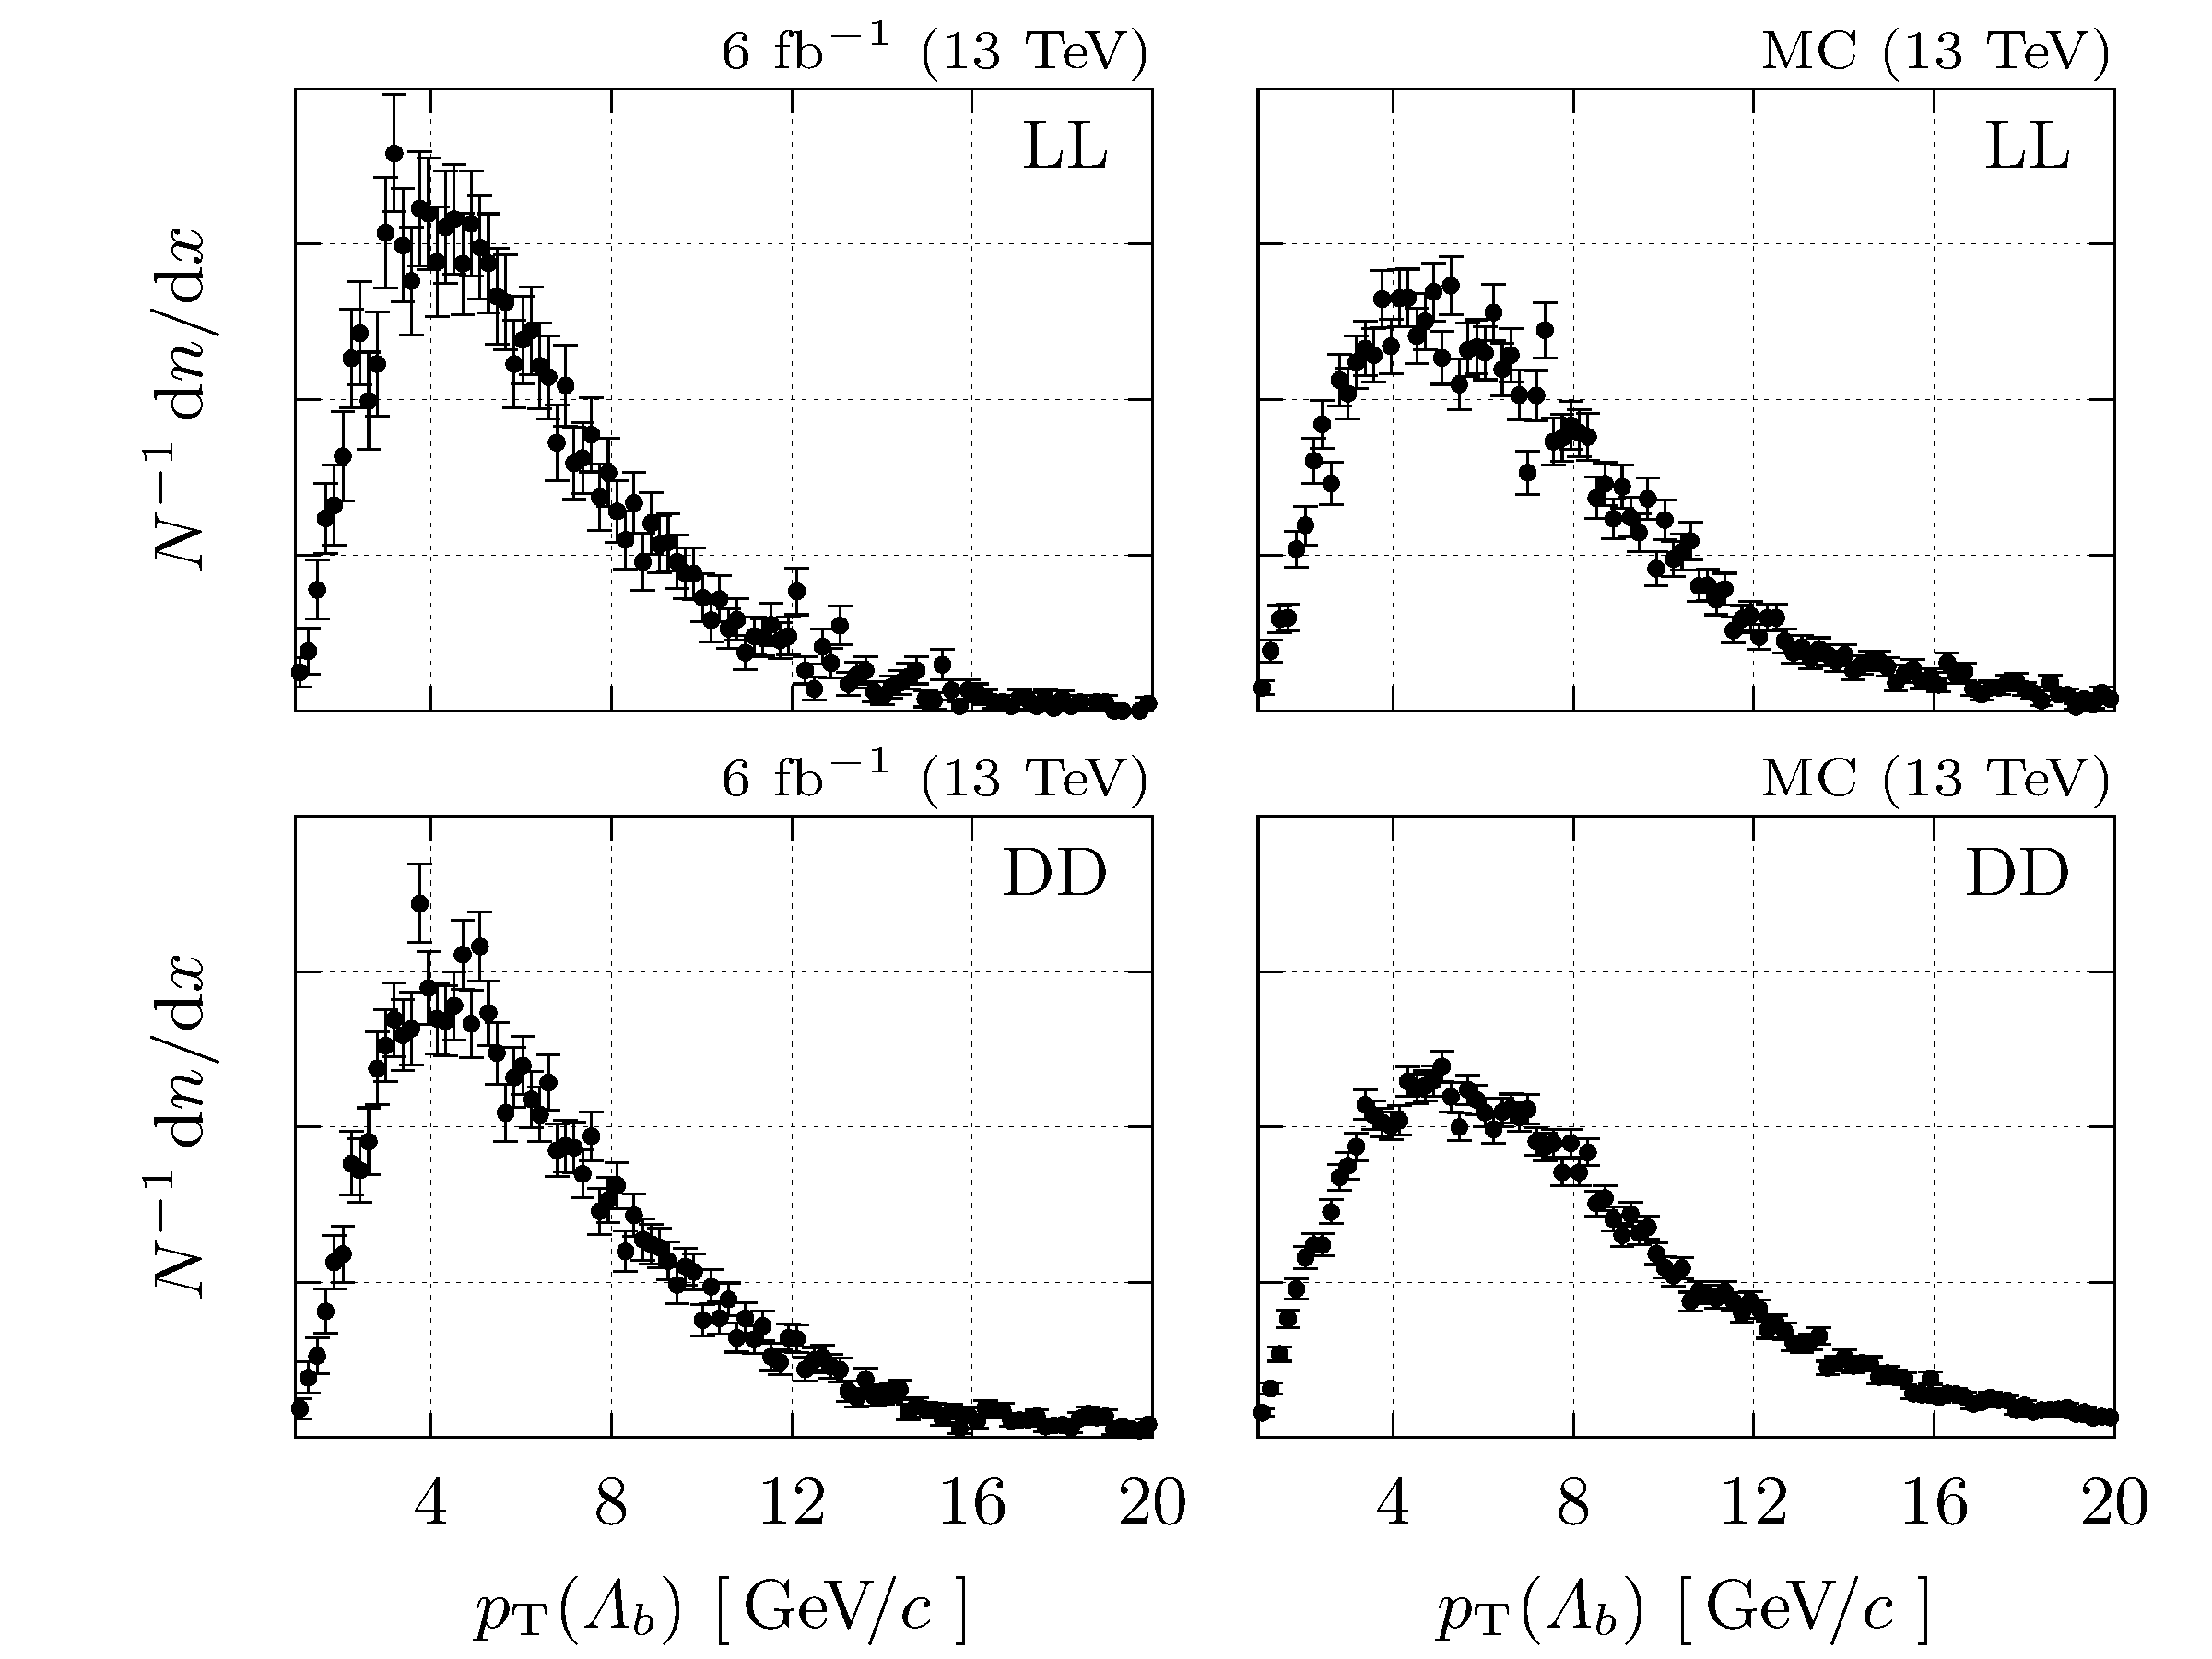
\includegraphics[scale=1.]{Lb2JpsiLz_weighting/hpT_corr.png}
    \caption{Distributions of the transverse momentum of the \Lb baryon for recorded data (left), simulated events (right) and different track types \gls{LL} and \gls{DD} (top and bottom) as obtained from sideband subtractions.}
    \label{fig:LbToJpsiLz_hpT_corr}
\end{figure}

\begin{figure}[htbp]
    \centering
    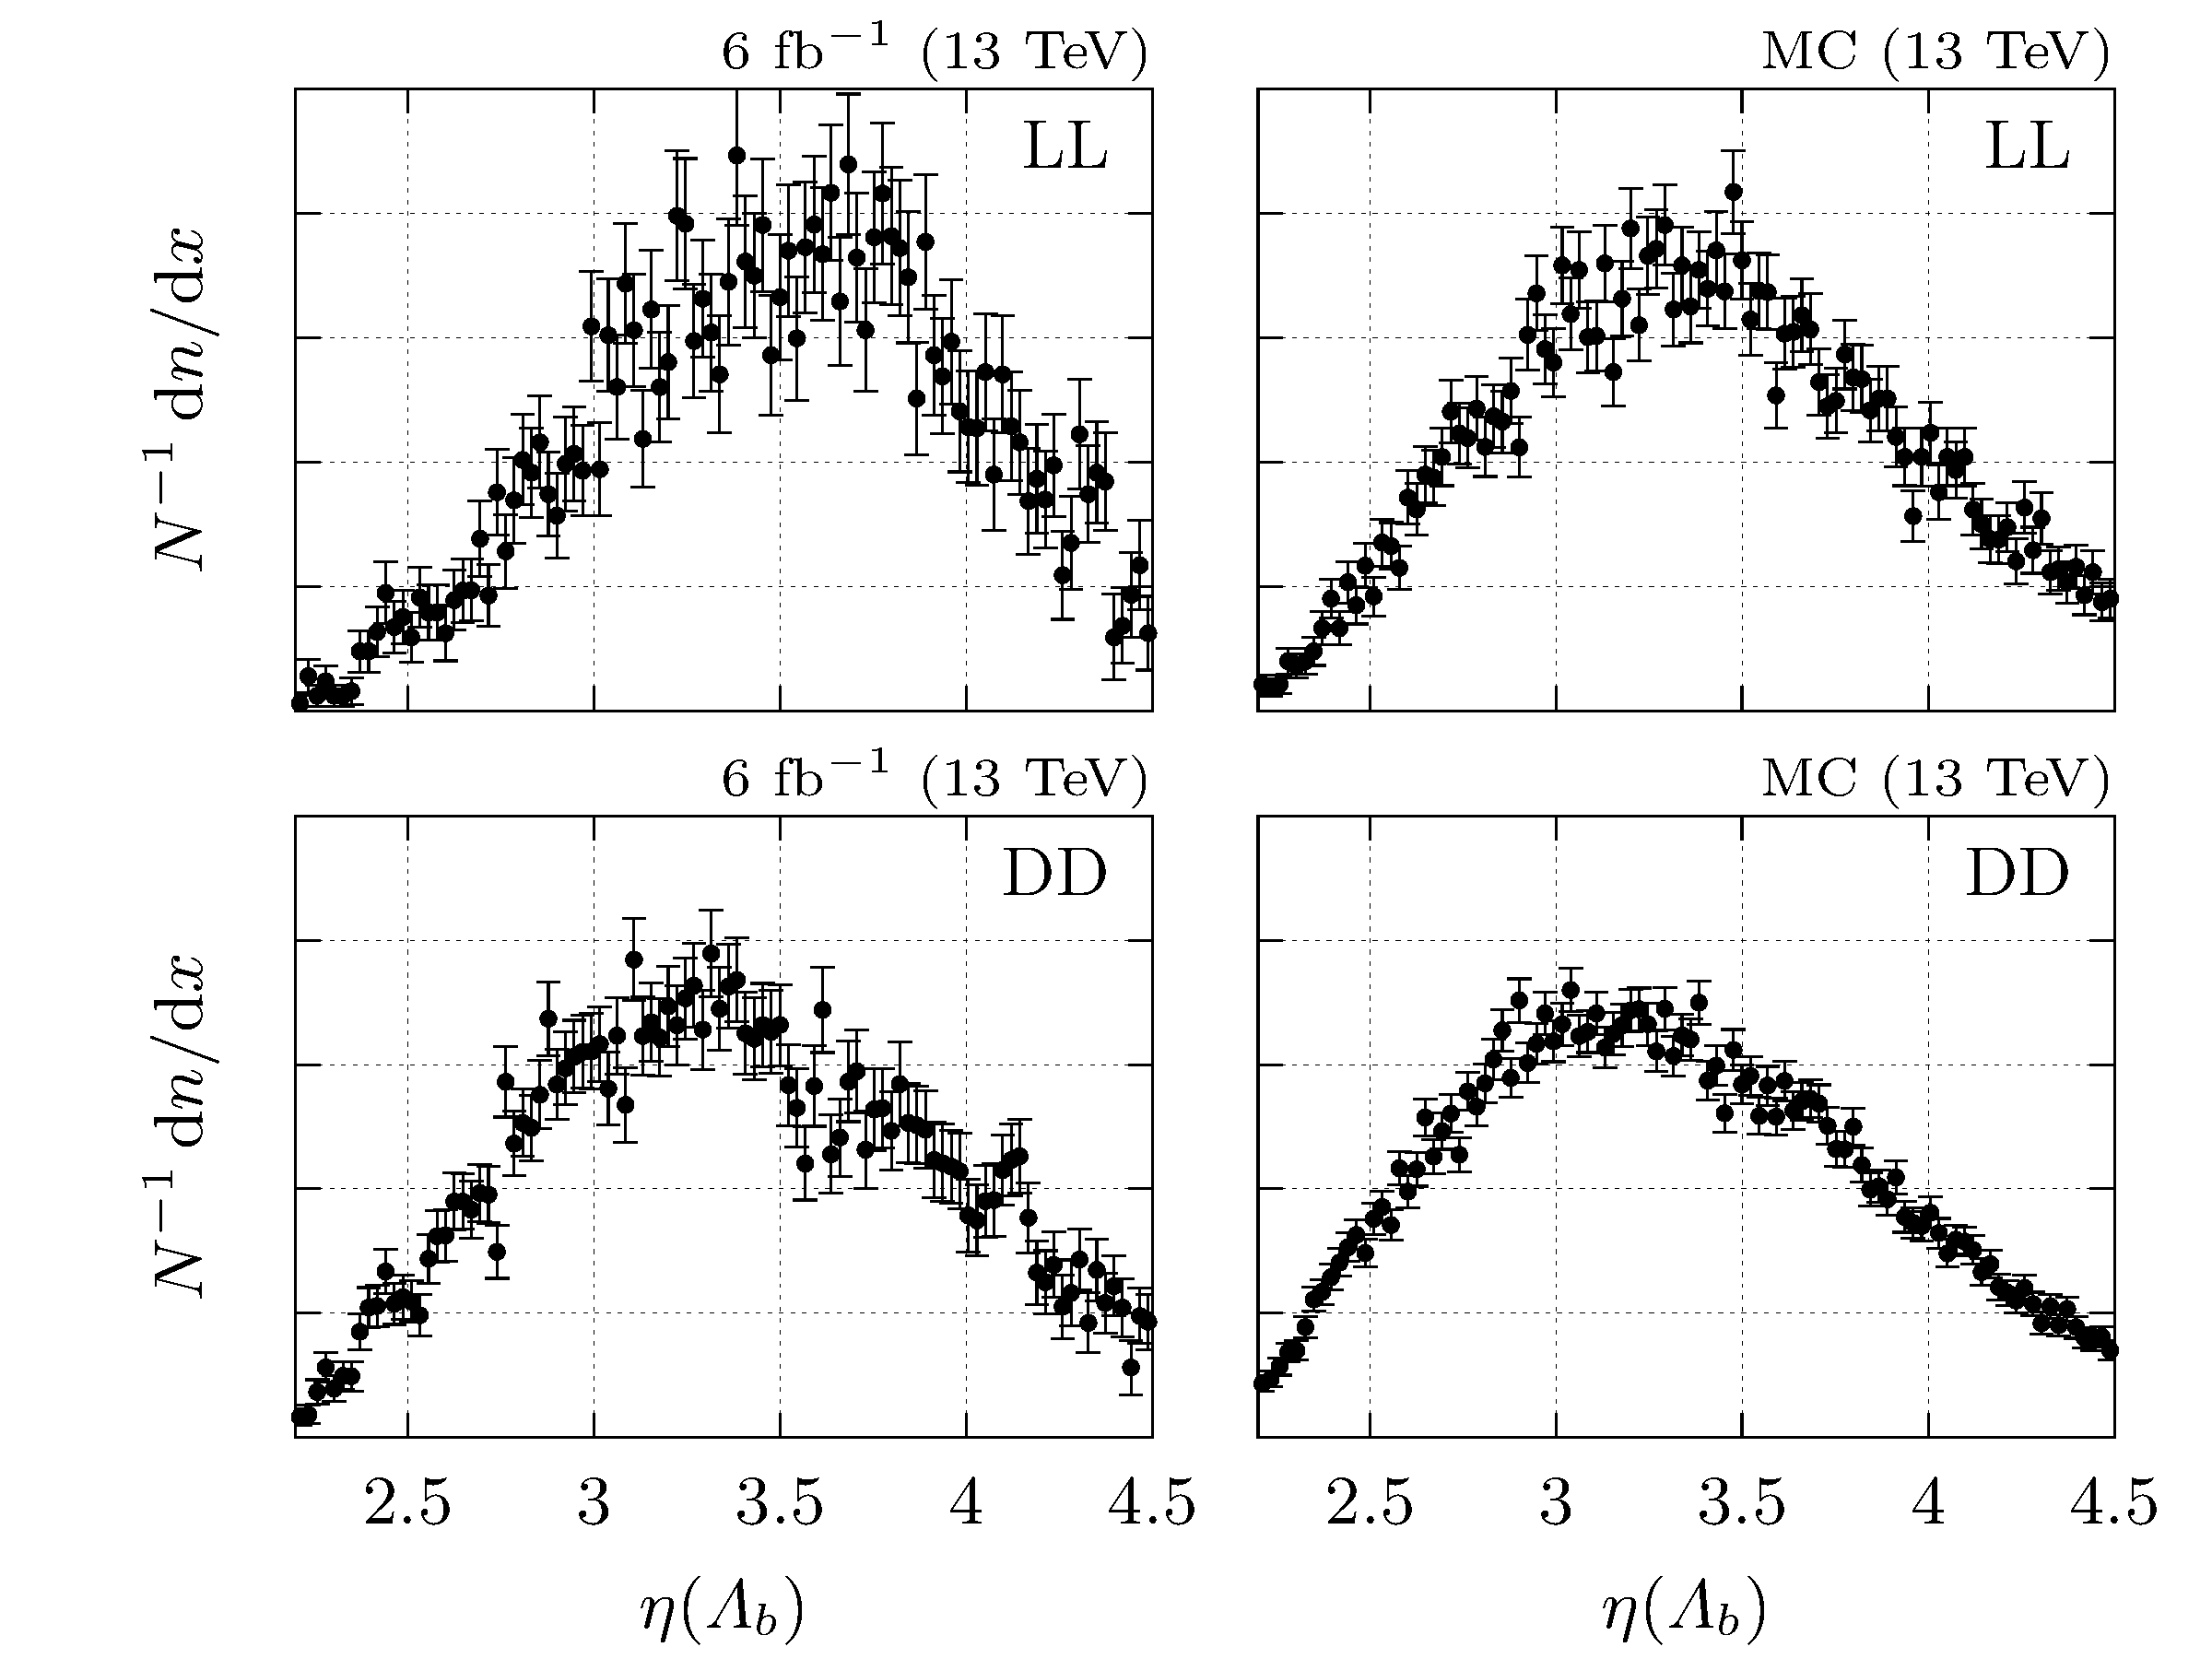
\includegraphics[scale=1.]{Lb2JpsiLz_weighting/heta_corr.png}
    \caption{Distributions of the pseudorapidity of the \Lb baryon for recorded data (left), simulated events (right) and different track types \gls{LL} and \gls{DD} (top and bottom) as obtained from sideband subtractions.}
    \label{fig:LbToJpsiLz_heta_corr}
\end{figure}

\begin{figure}[htbp]
    \centering
    \begin{subfigure}{\textwidth}
        \centering
        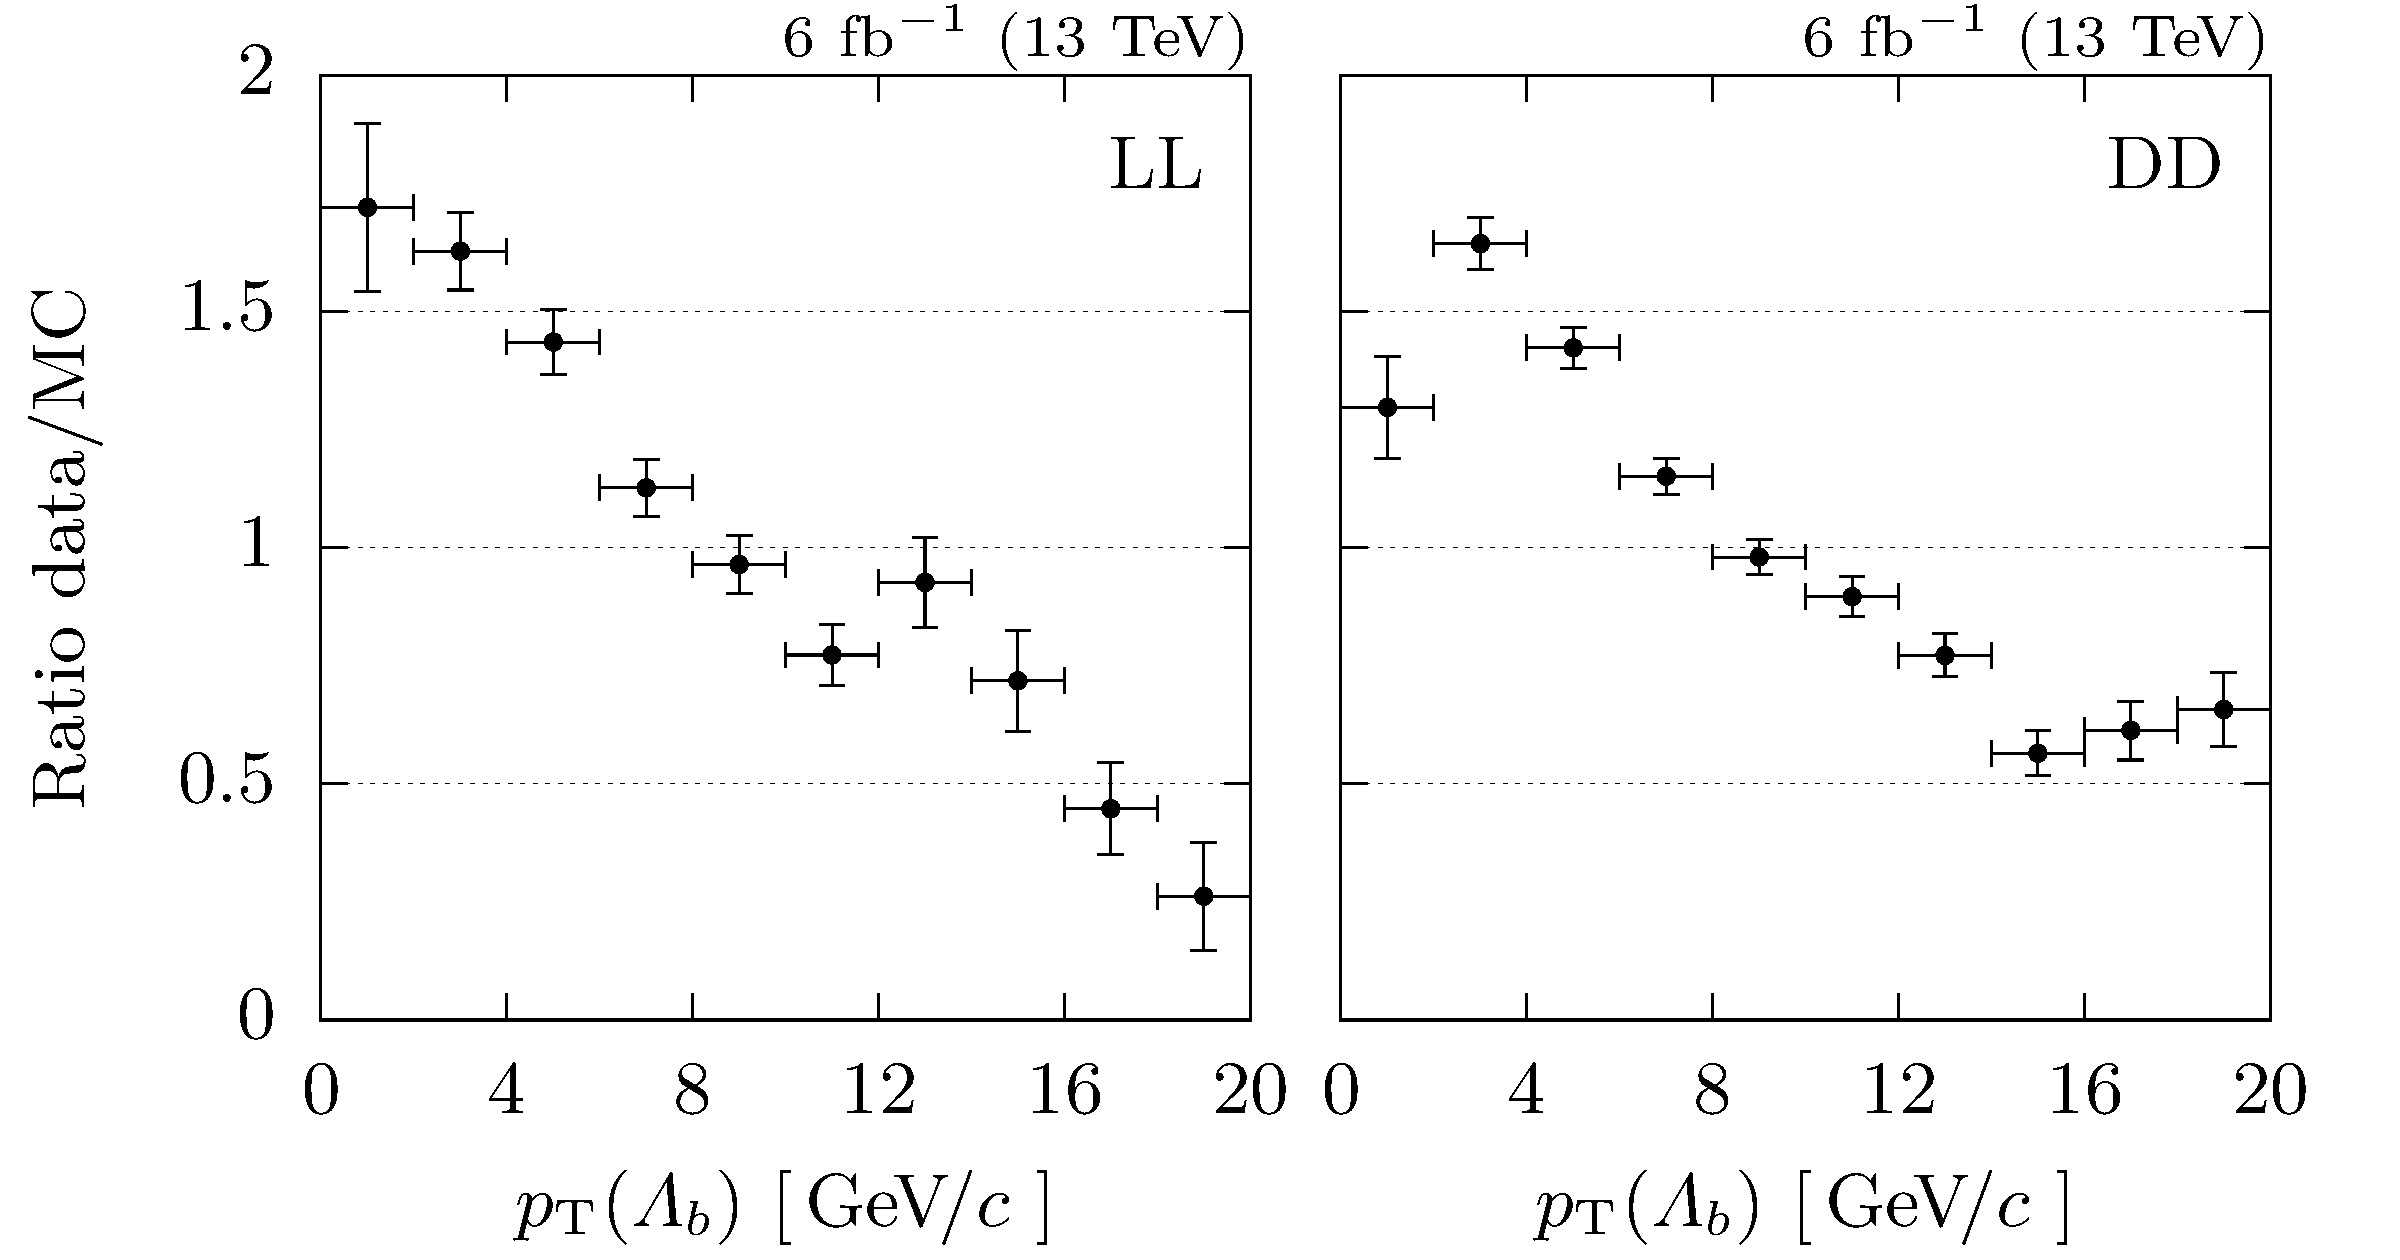
\includegraphics[scale=1.]{Lb2JpsiLz_weighting/hratio_pT.png}
    \end{subfigure}
    \par\bigskip 
    \begin{subfigure}{\textwidth}
        \centering
        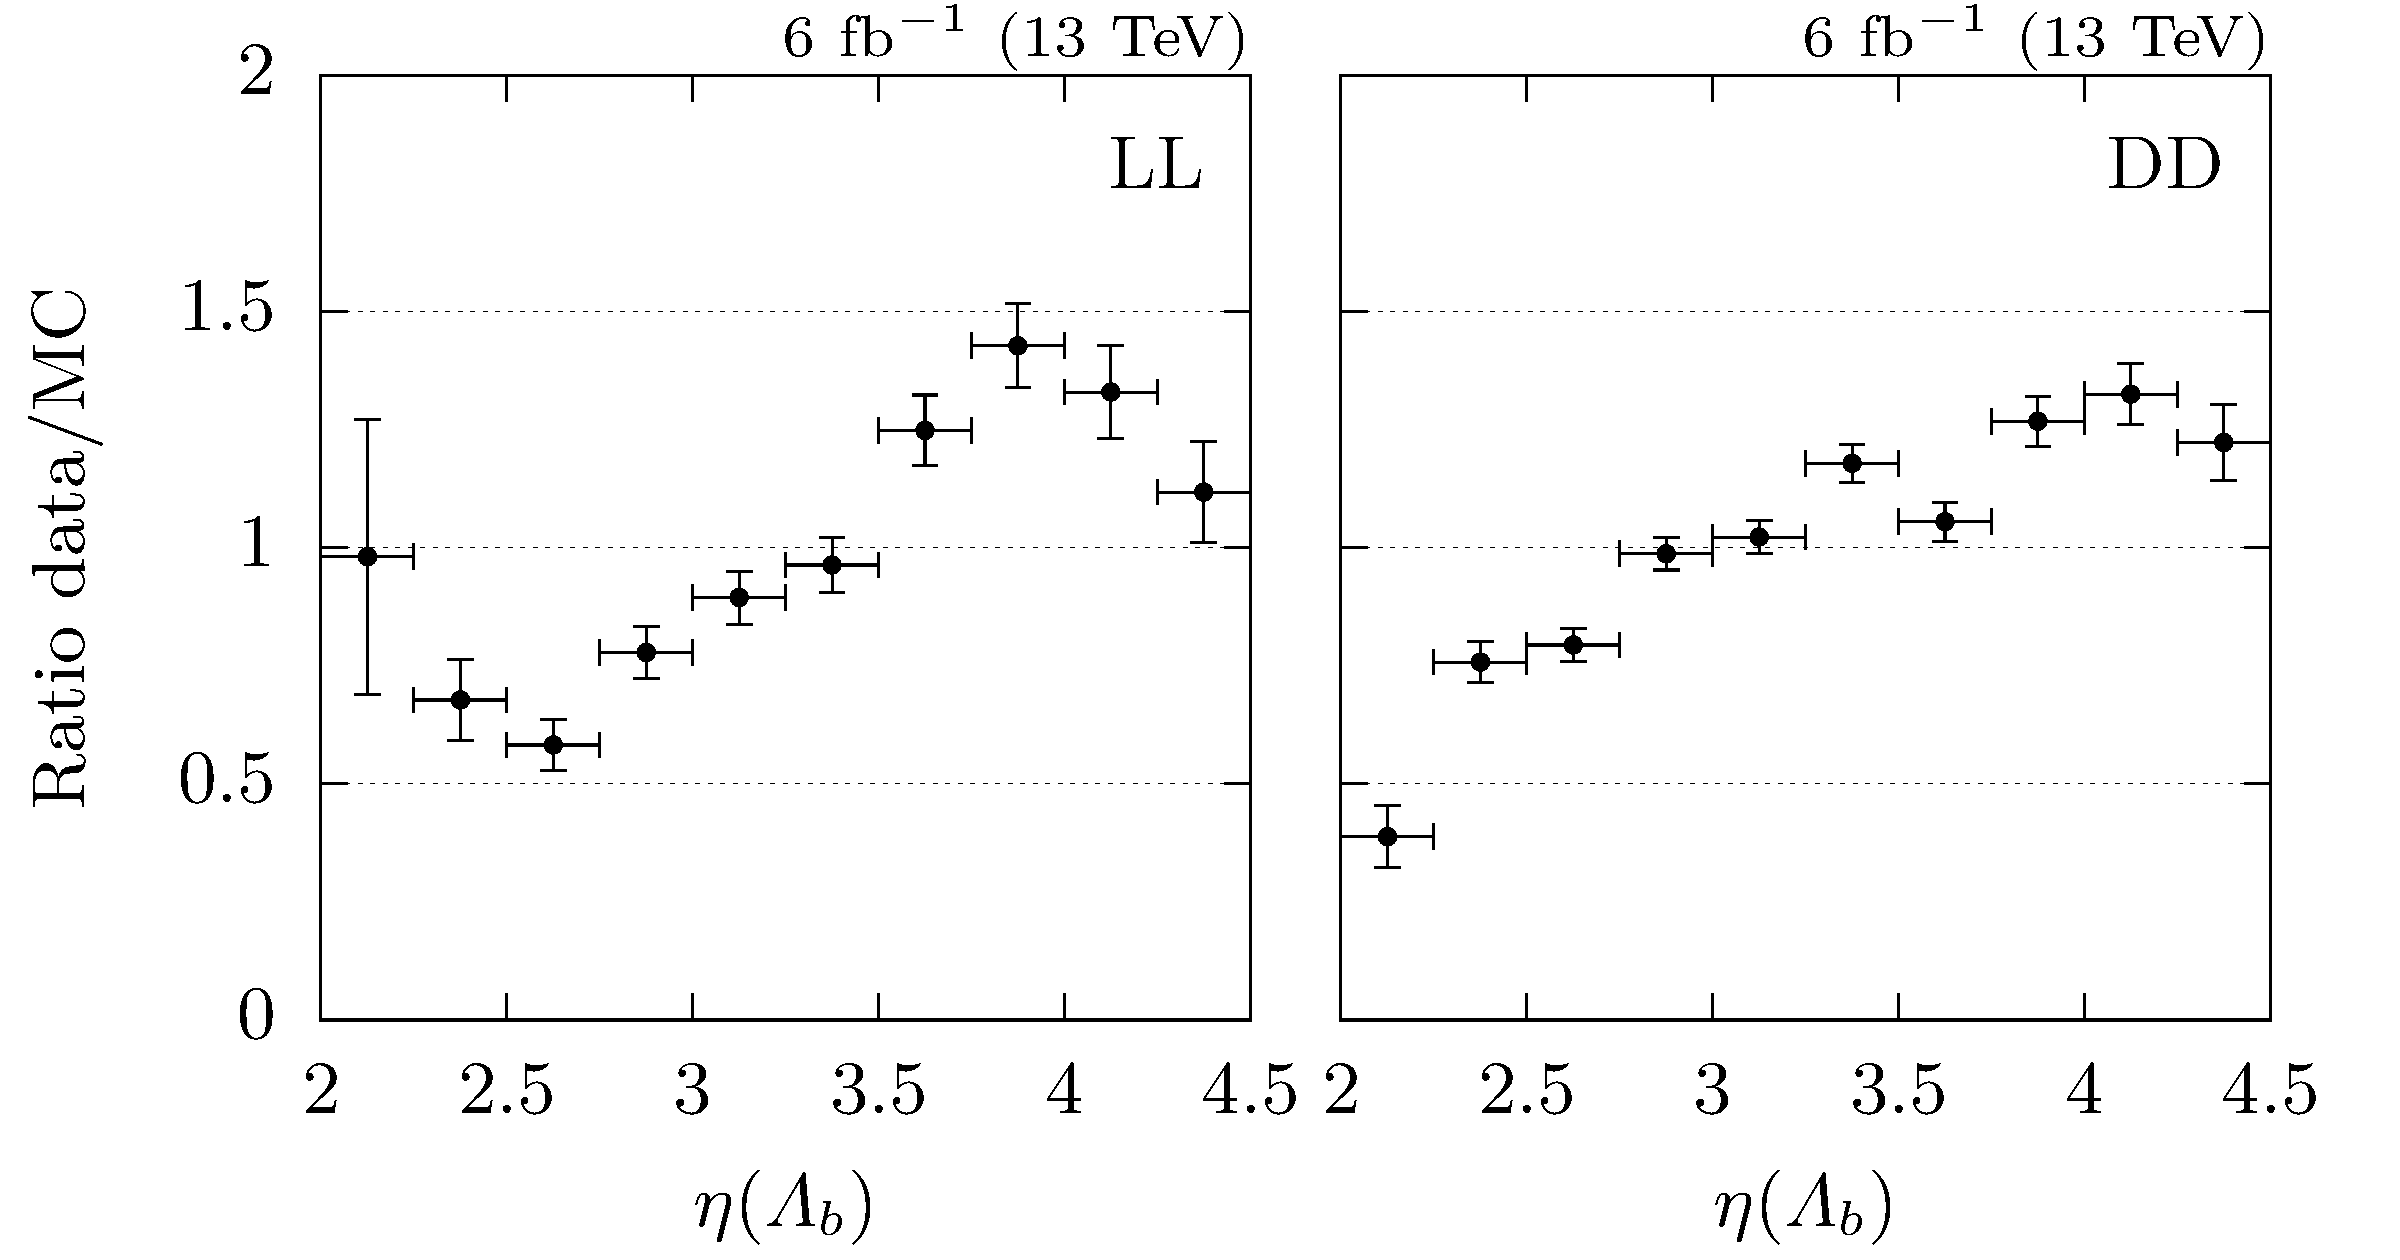
\includegraphics[scale=1.]{Lb2JpsiLz_weighting/hratio_eta.png}
    \end{subfigure}
    \par\bigskip 
    \begin{subfigure}{\textwidth}
        \centering
        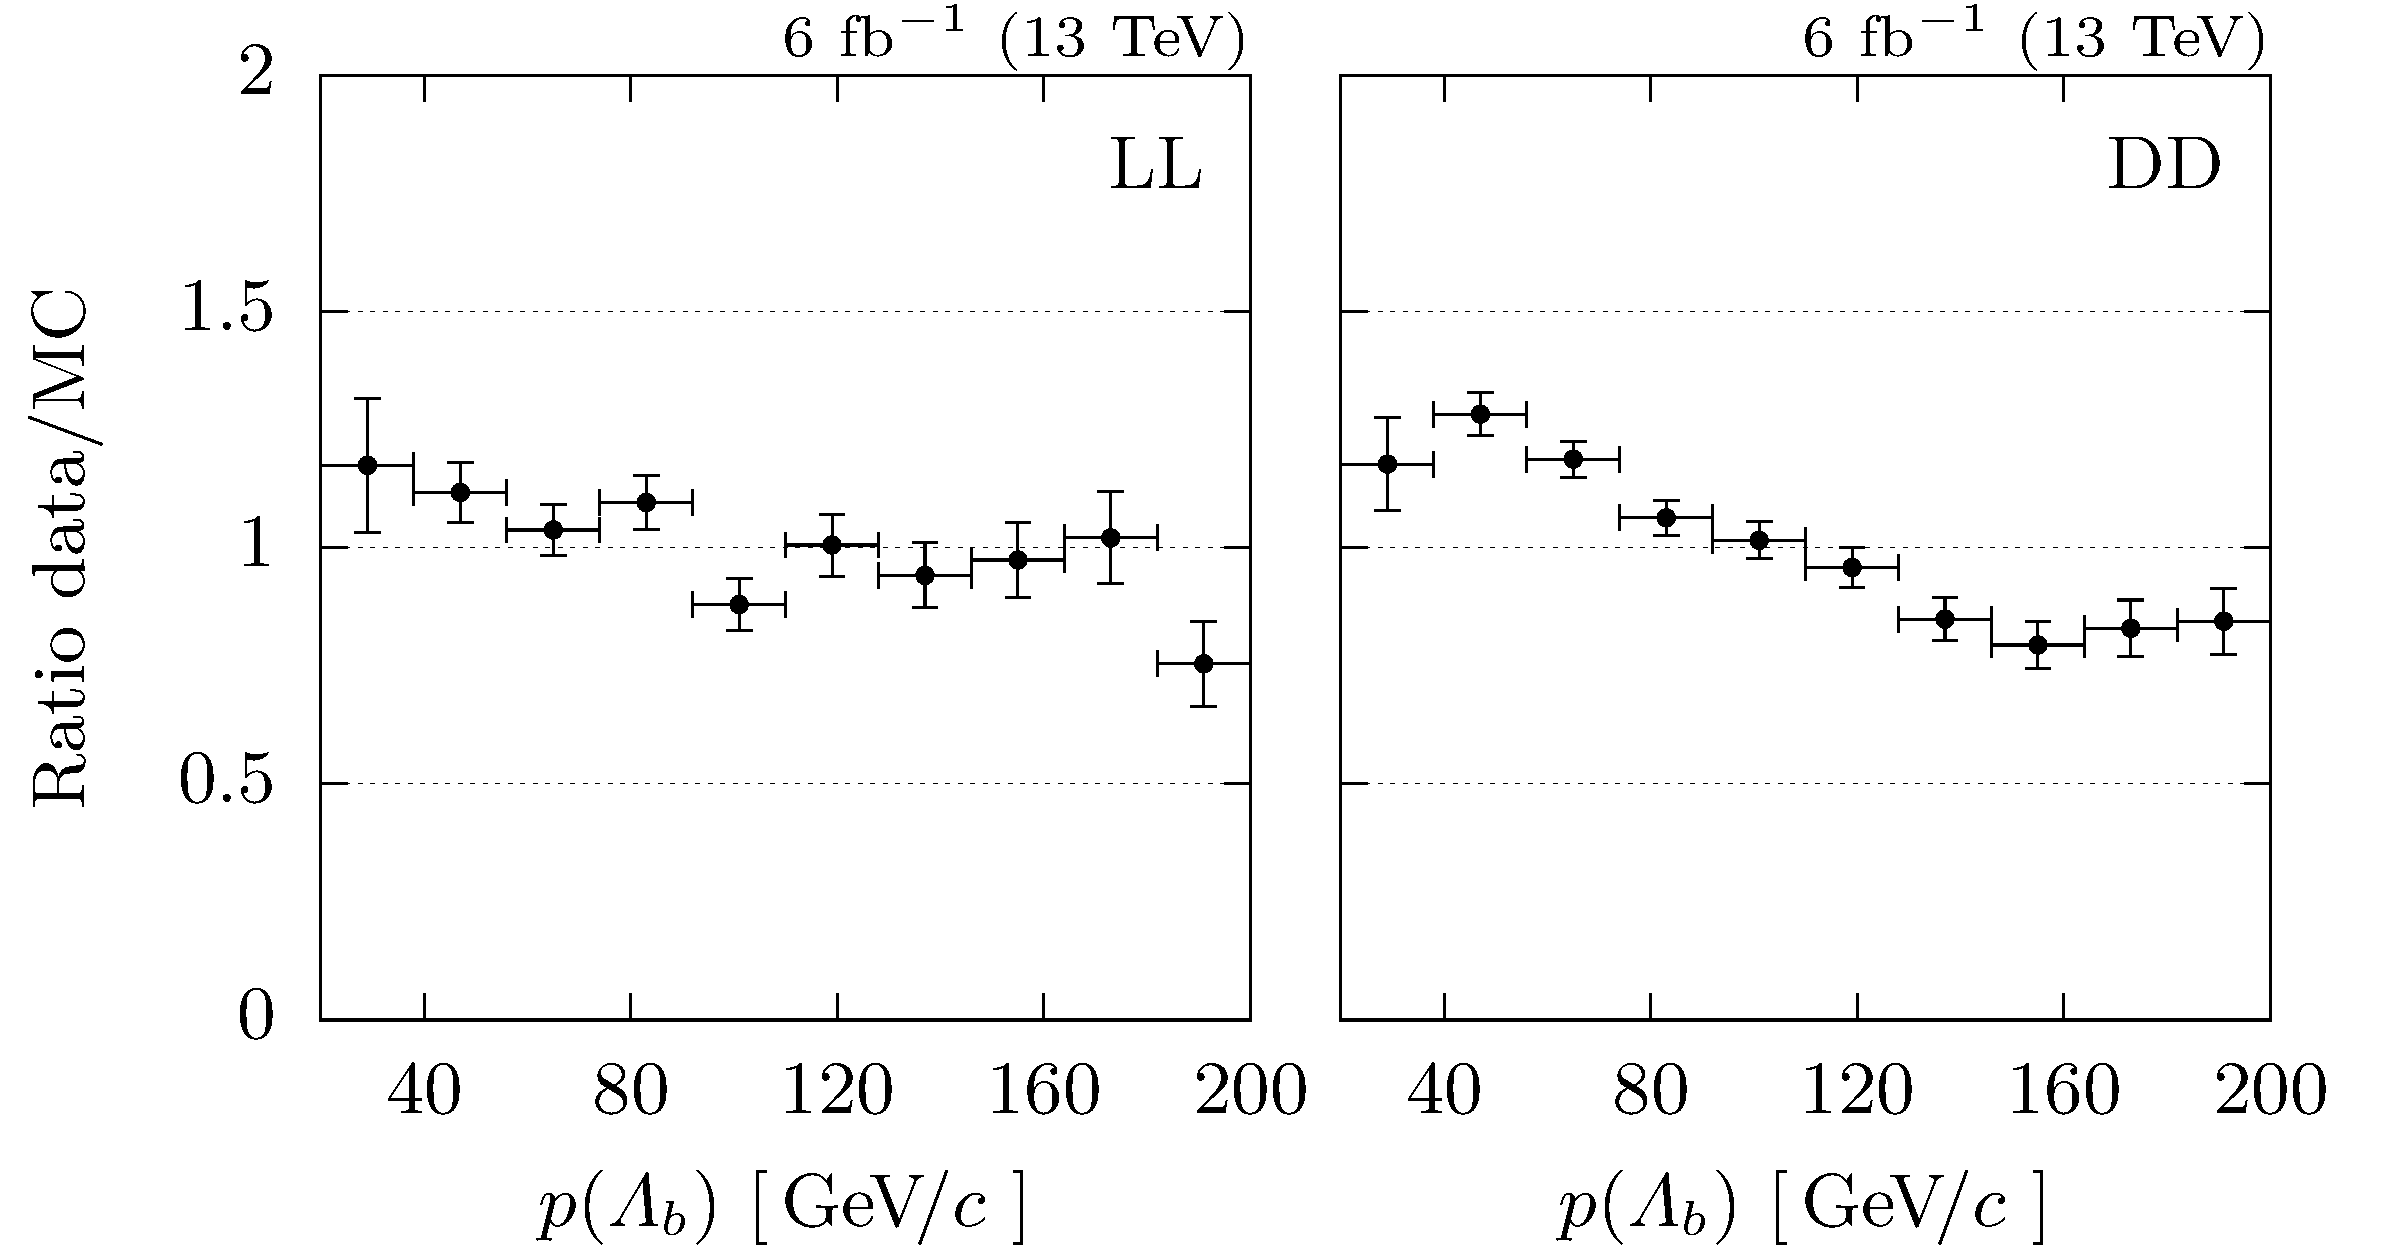
\includegraphics[scale=1.]{Lb2JpsiLz_weighting/hratio_p.png}
    \end{subfigure}
    \par\bigskip 
    \caption{Ratio of the (binned) distributions of the transverse momentum (top), pseudorapidity (middle) and three-momentum magnitude (bottom) of the \Lb baryon for recorded data and \gls{mc} simulated events. The ratios are split w.r.t.\ the track types \gls{LL} (left) and \gls{DD} (right).}
    \label{fig:LbToJpsiLz_hratio}
\end{figure}

After taking the ratios, the histograms are normalized to unity such that in case of a common underlying distribution every bin entry should be one (within uncertainty).
The distributions of the ratios show that this is neither the case for $\pt(\Lb)$ and $\eta(\Lb)$, nor for $p(\Lb)$.
This deviation is expected and motivates the recalibration of the \gls{mc} simulated events with weights.
In the following we will use the distribution of the three-momentum magnitude $p(\Lb)$ to benchmark the performance of the calibration.
If recorded data and simulated events follow the same underlying distribution, the sum
\begin{equation*}
    \chi^2 \equiv \sum_{i=1}^n \chi_i^2
\end{equation*}
of the normalized deviation from one $\chi_i^2$ for each bin $i$,
\begin{equation*}
    \chi_i^2 \equiv \left( \frac{r_i - 1}{u(r_i)} \right)^2 \,,
\end{equation*}
where $r_i$ and $u(r_i)$ is the central value and its uncertainty of the $i$-th bin, respectively, is then $\chi^2$-distributed with $n$ \gls{dof} (number of bins).
For \gls{LL} (\gls{DD}) we find $\chi^2 \approx 21$ ($\chi^2 \approx 109$) and thus reject the hypothesis of a common underlying distribution for recorded data and simulated events on a $>98\,\%$ confidence level according to Eq.~\eqref{eq:fitprob}.

Weights are calculated by taking the binned, normalized ratio of the marginal distributions of recorded and simulated events for \pt or $\eta$ in subsequent steps.
The data set is split w.r.t.\ the track types \gls{LL} and \gls{DD}.
The resulting histograms of ratios $w_1(\pt)$ and $w_2(\eta)$, binned for the given quantity \pt and $\eta$, are then used to calculated the \pt and $\eta$ dependent weight $w(\pt, \eta) := w_1(\pt) \times w_2(\eta)$ for a given simulated event.
The iteration procedure is structured as following:
\begin{enumerate}[itemsep=2pt,parsep=2pt]
    \item Initialize all weights with one.
    \item Update $w_1(\pt)$ using weight factors from the previous iteration.
    \item Update $w(\pt, \eta) = w_1(\pt) \times w_2(\eta)$.
    \item Update $w_2(\eta)$ using the updated $w_1(\pt)$ and $w_2(\eta)$ from the previous iteration.
    \item Update $w(\pt, \eta) = w_1(\pt) \times w_2(\eta)$.
    \item Continue with step 2 until convergence is reached. 
\end{enumerate}
%By design, at the end of each iteration, the ratio of recorded data and weighted simulated events should be one in the marginal distribution of $\eta(\Lb)$.
Each iteration yields a factor $w_1(\pt)$ and $w_2(\eta)$ for a given \pt and $\eta$ bin.
The final weights are their product.
%, \ie{}, $$w(\pt, \eta) = w_1(\pt) \times w_2(\eta).$$
The convergence of this approach is measured in the weight update for each bin, separately.

Starting from the first iteration the histograms for (weighted) simulated events are filled with tuples of the particle event with an associated weight $(x_i, w_i)$.
After filling, the content of a bin~$j$ is the sum of its weights~$w^{(j)}_i$ and the associated uncertainty~$u^{(j)}$ is
\begin{equation*}
    u^{(j)} = \sqrt{ \sum_i \left( w^{(j)}_i \right)^2 } \,.
\end{equation*}
We note that for $w^{(j)}_i = 1~\forall i,j$ this scheme is equivalent to unweighted events where the uncertainty of each bin with bin content $n$ is given by $\sqrt n$.

\begin{figure}[htbp]
    \centering
    \begin{subfigure}{\textwidth}
        \centering
        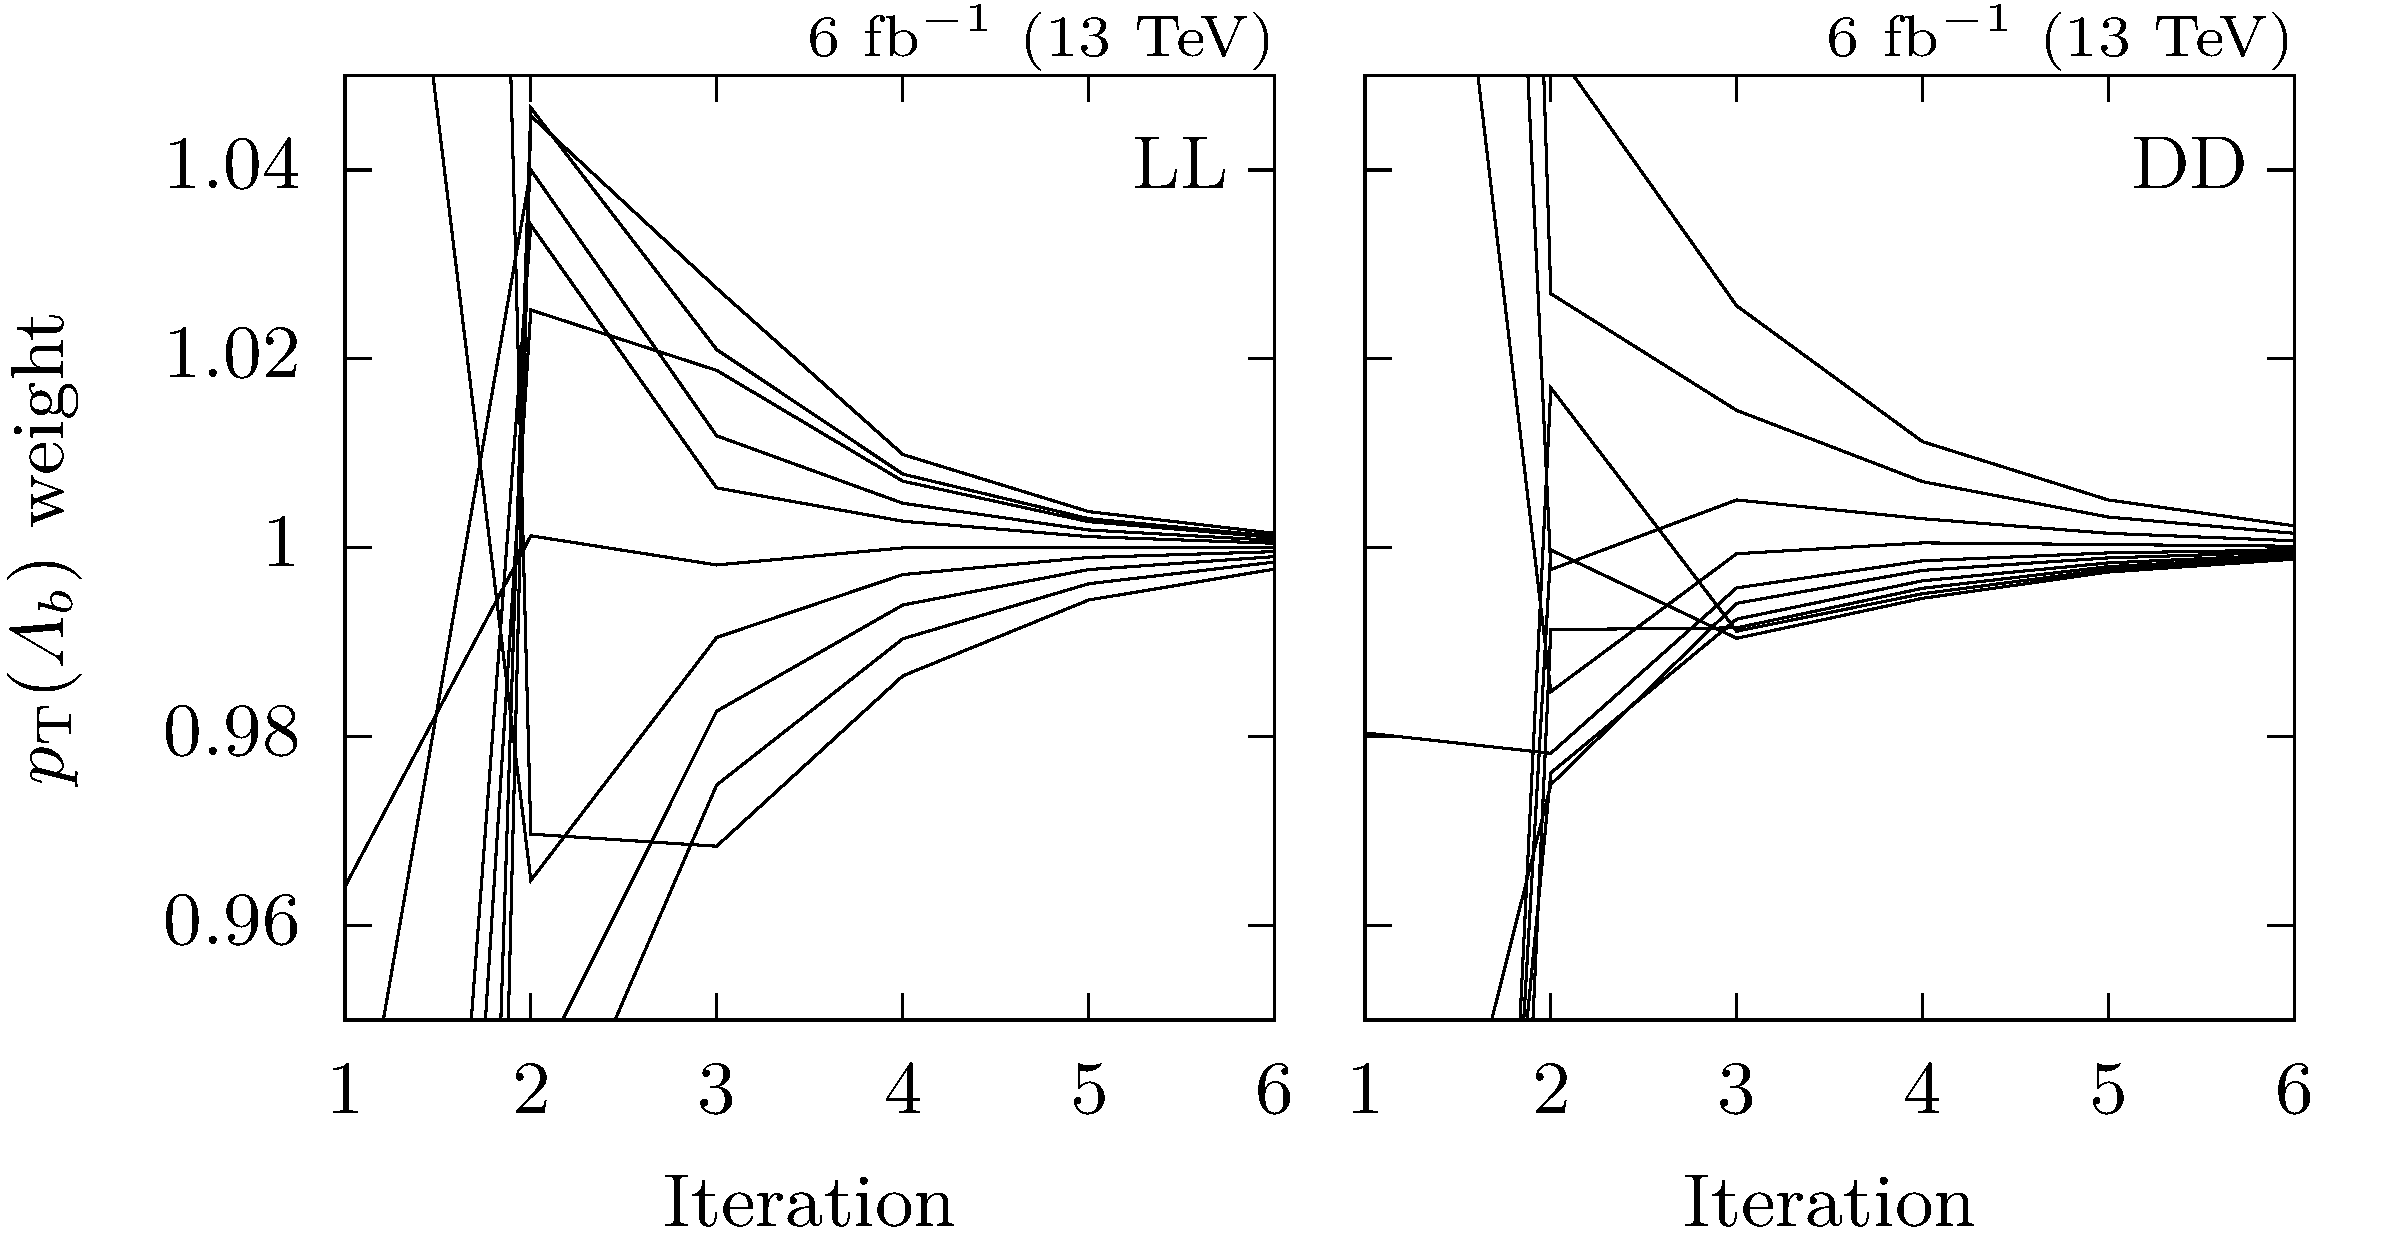
\includegraphics[scale=1.]{Lb2JpsiLz_weighting/conv_pT.png}
    \end{subfigure}
    \par\bigskip 
    \begin{subfigure}{\textwidth}
        \centering
        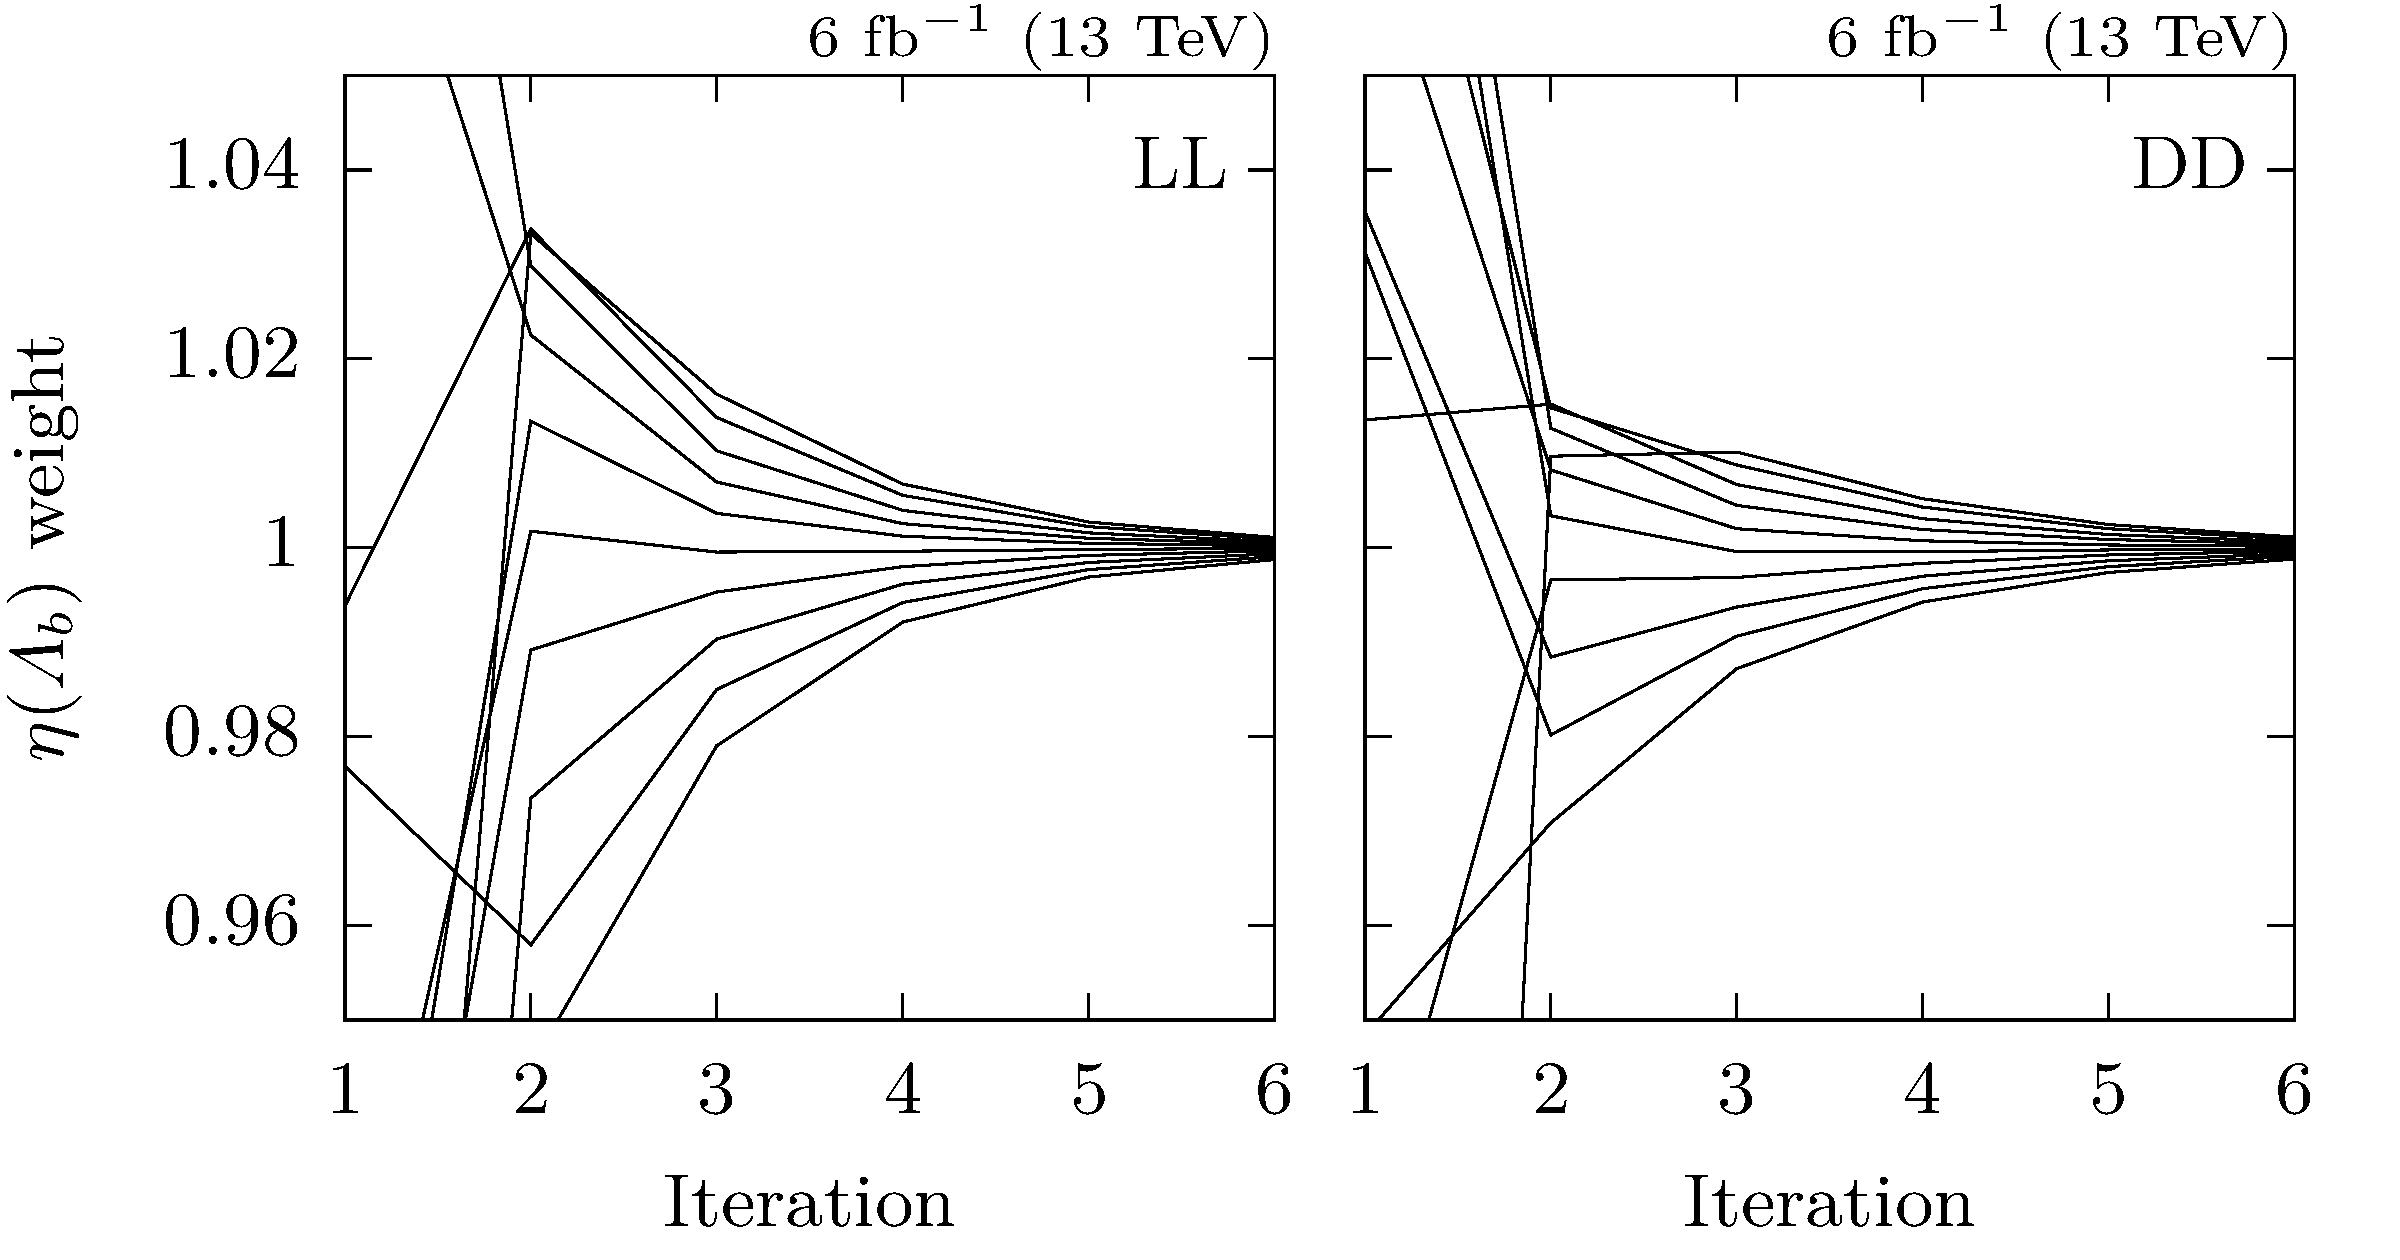
\includegraphics[scale=1.]{Lb2JpsiLz_weighting/conv_eta.png}
    \end{subfigure}
    \caption{Convergence of $w_1(\pt)$ (top) and $w_2(\eta)$ (bottom) during the iterative weighting process for \gls{LL} and \gls{DD} tracks (left and right).}
    \label{fig:LbToJpsiLz_conv}
\end{figure}

In Fig.~\ref{fig:LbToJpsiLz_conv} we show the convergence of the iterative weighting process for \gls{LL} and \gls{DD} tracks.
Each solid line is the weight update of a bin as a function of the iteration number.
Convergence is achieved when all multiplicative updates have approached the value one.
In the above case, we stop the iteration after six iterations and consider the product of all weight updates (starting with the value one of the zeroth iteration) as the converged final weight for each bin.

The significance of the obtained weights is quantized in the $p$-values corresponding to the hypothesis of a common underlying distribution for recorded and simulated events, \ie{}, $w_1(p_T)=1$ and $w_2(\eta)=1$, respectively.
These $p$-values are listed in Tab.~\ref{tab:LbToJpsiLz_pvalues} after six successive iterations.
Incompatibilities with these hypotheses are expected and indicate the necessity of the scaling process, whereas the $p$-value for $r(p)=1$, where $r(p)$ is the (binned) ratio of the three-momentum magnitude distribution of recorded data and simulated events, exhibits the improvement of features that are scaled implicitly due to correlations with \pt and $\eta$.
The change of $r(p)$ during the iterations is also listed in Tab.~\ref{tab:LbToJpsiLz_pvalues} and shows the improvement of the fidelity of the \gls{mc} simulated events due to the scaling with $w(\pt,\eta)$.

%\begin{figure}[htbp]
%    \centering
%    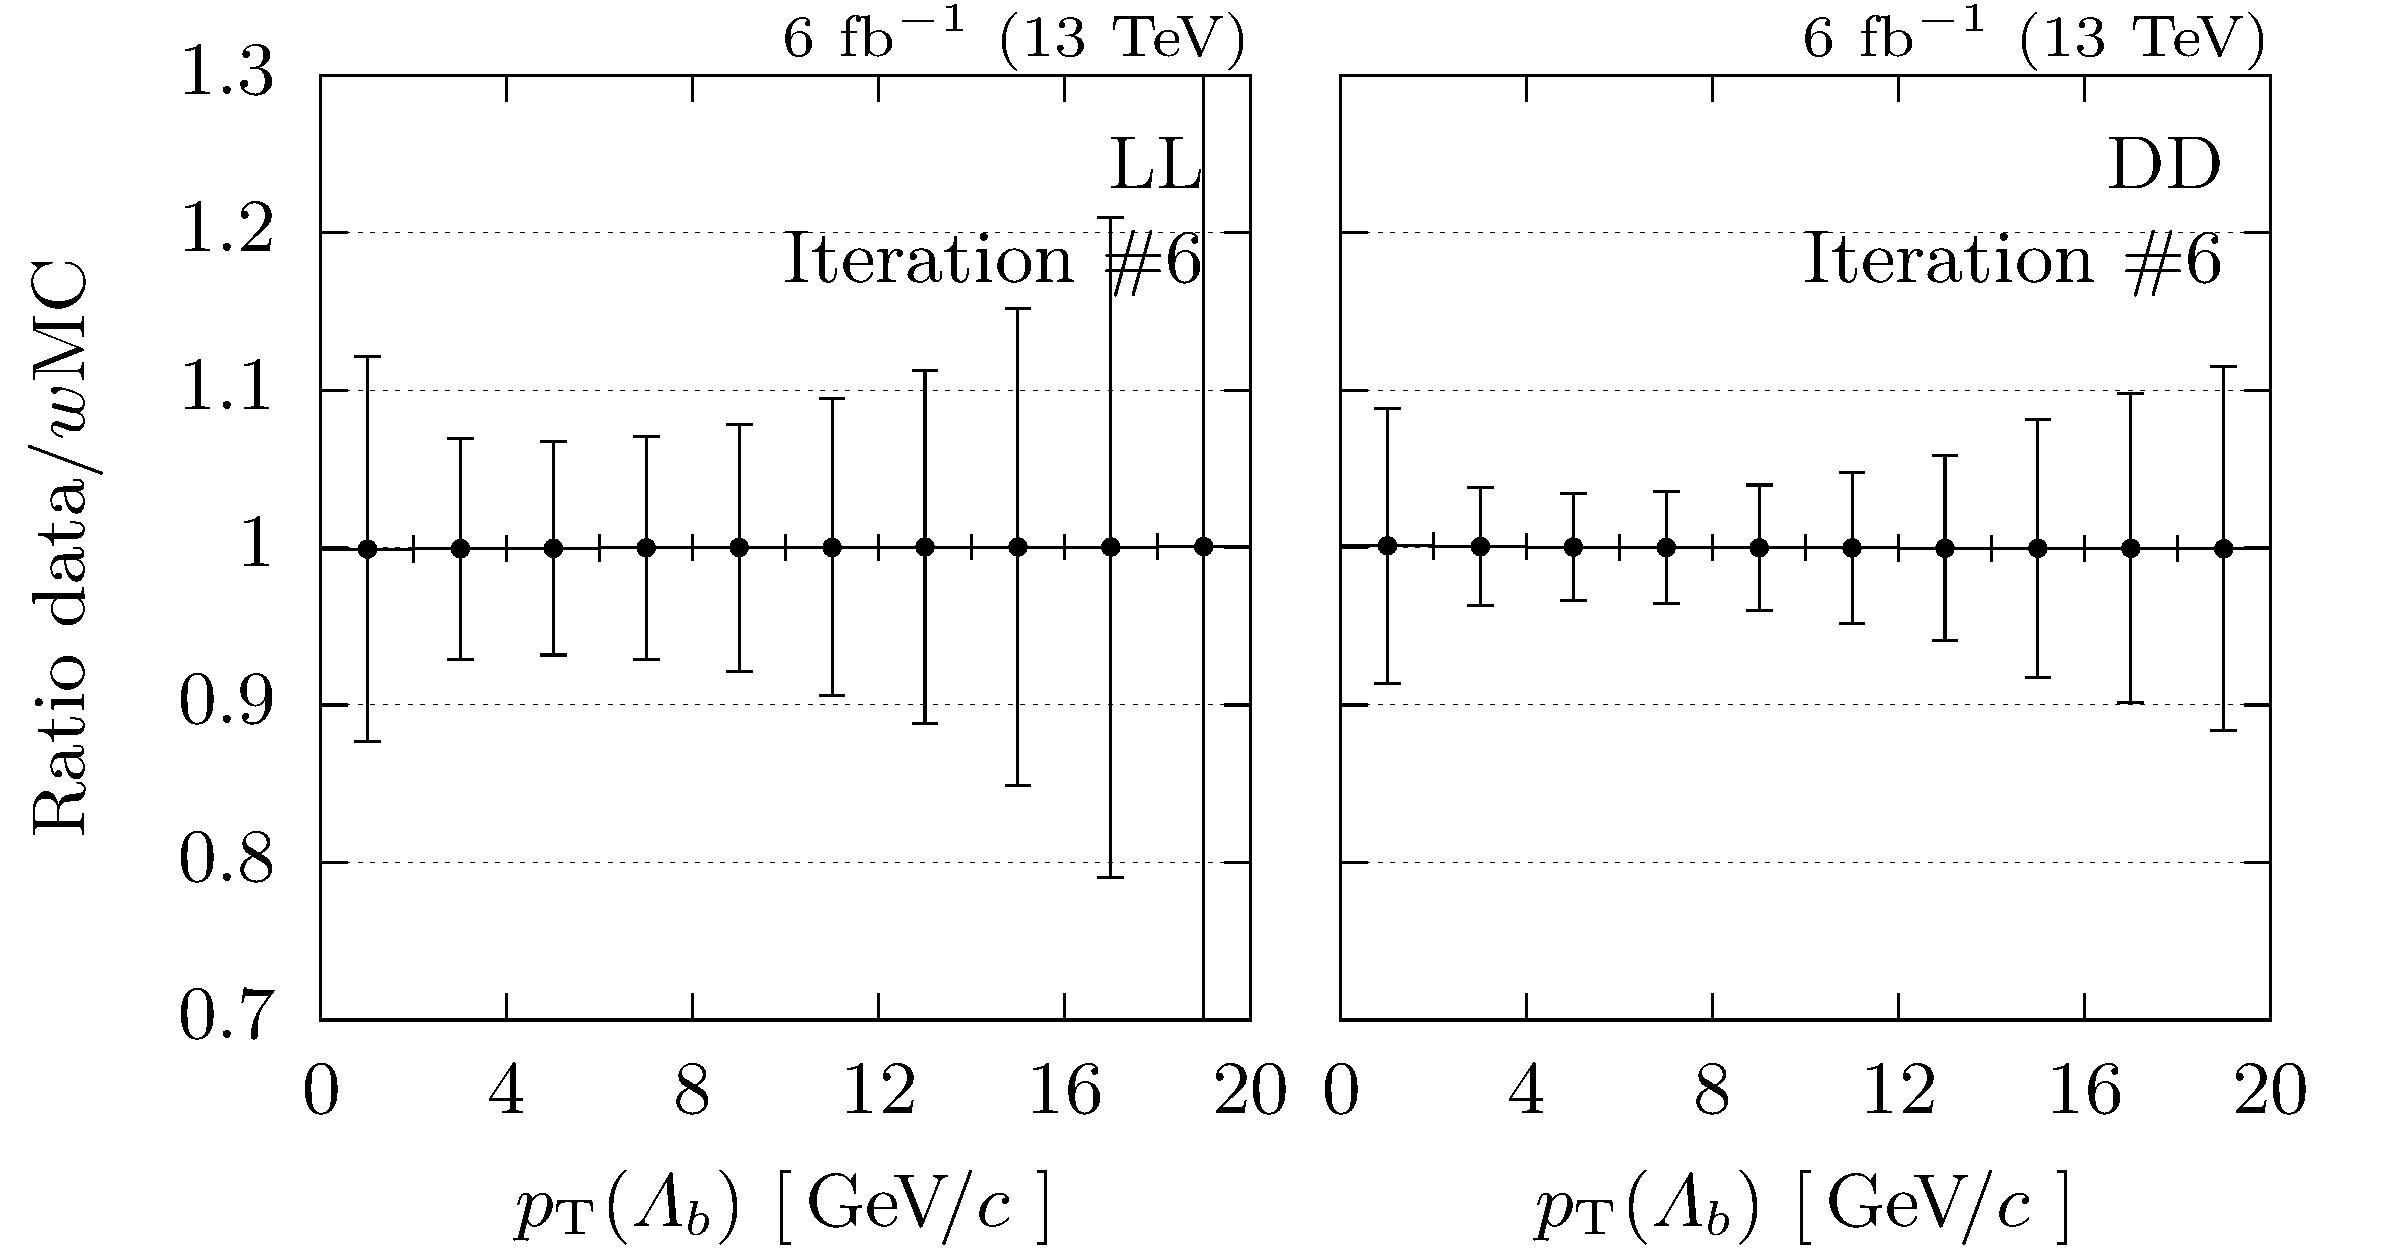
\includegraphics[scale=1.]{Lb2JpsiLz_weighting/hratio_pT_final.png}
%    \caption{Ratio of recorded data and weighted MC simulated events after six successive iterations in $\pt(\Lb)$ bins.}
%\end{figure}

%\begin{figure}[htbp]
%    \centering
%    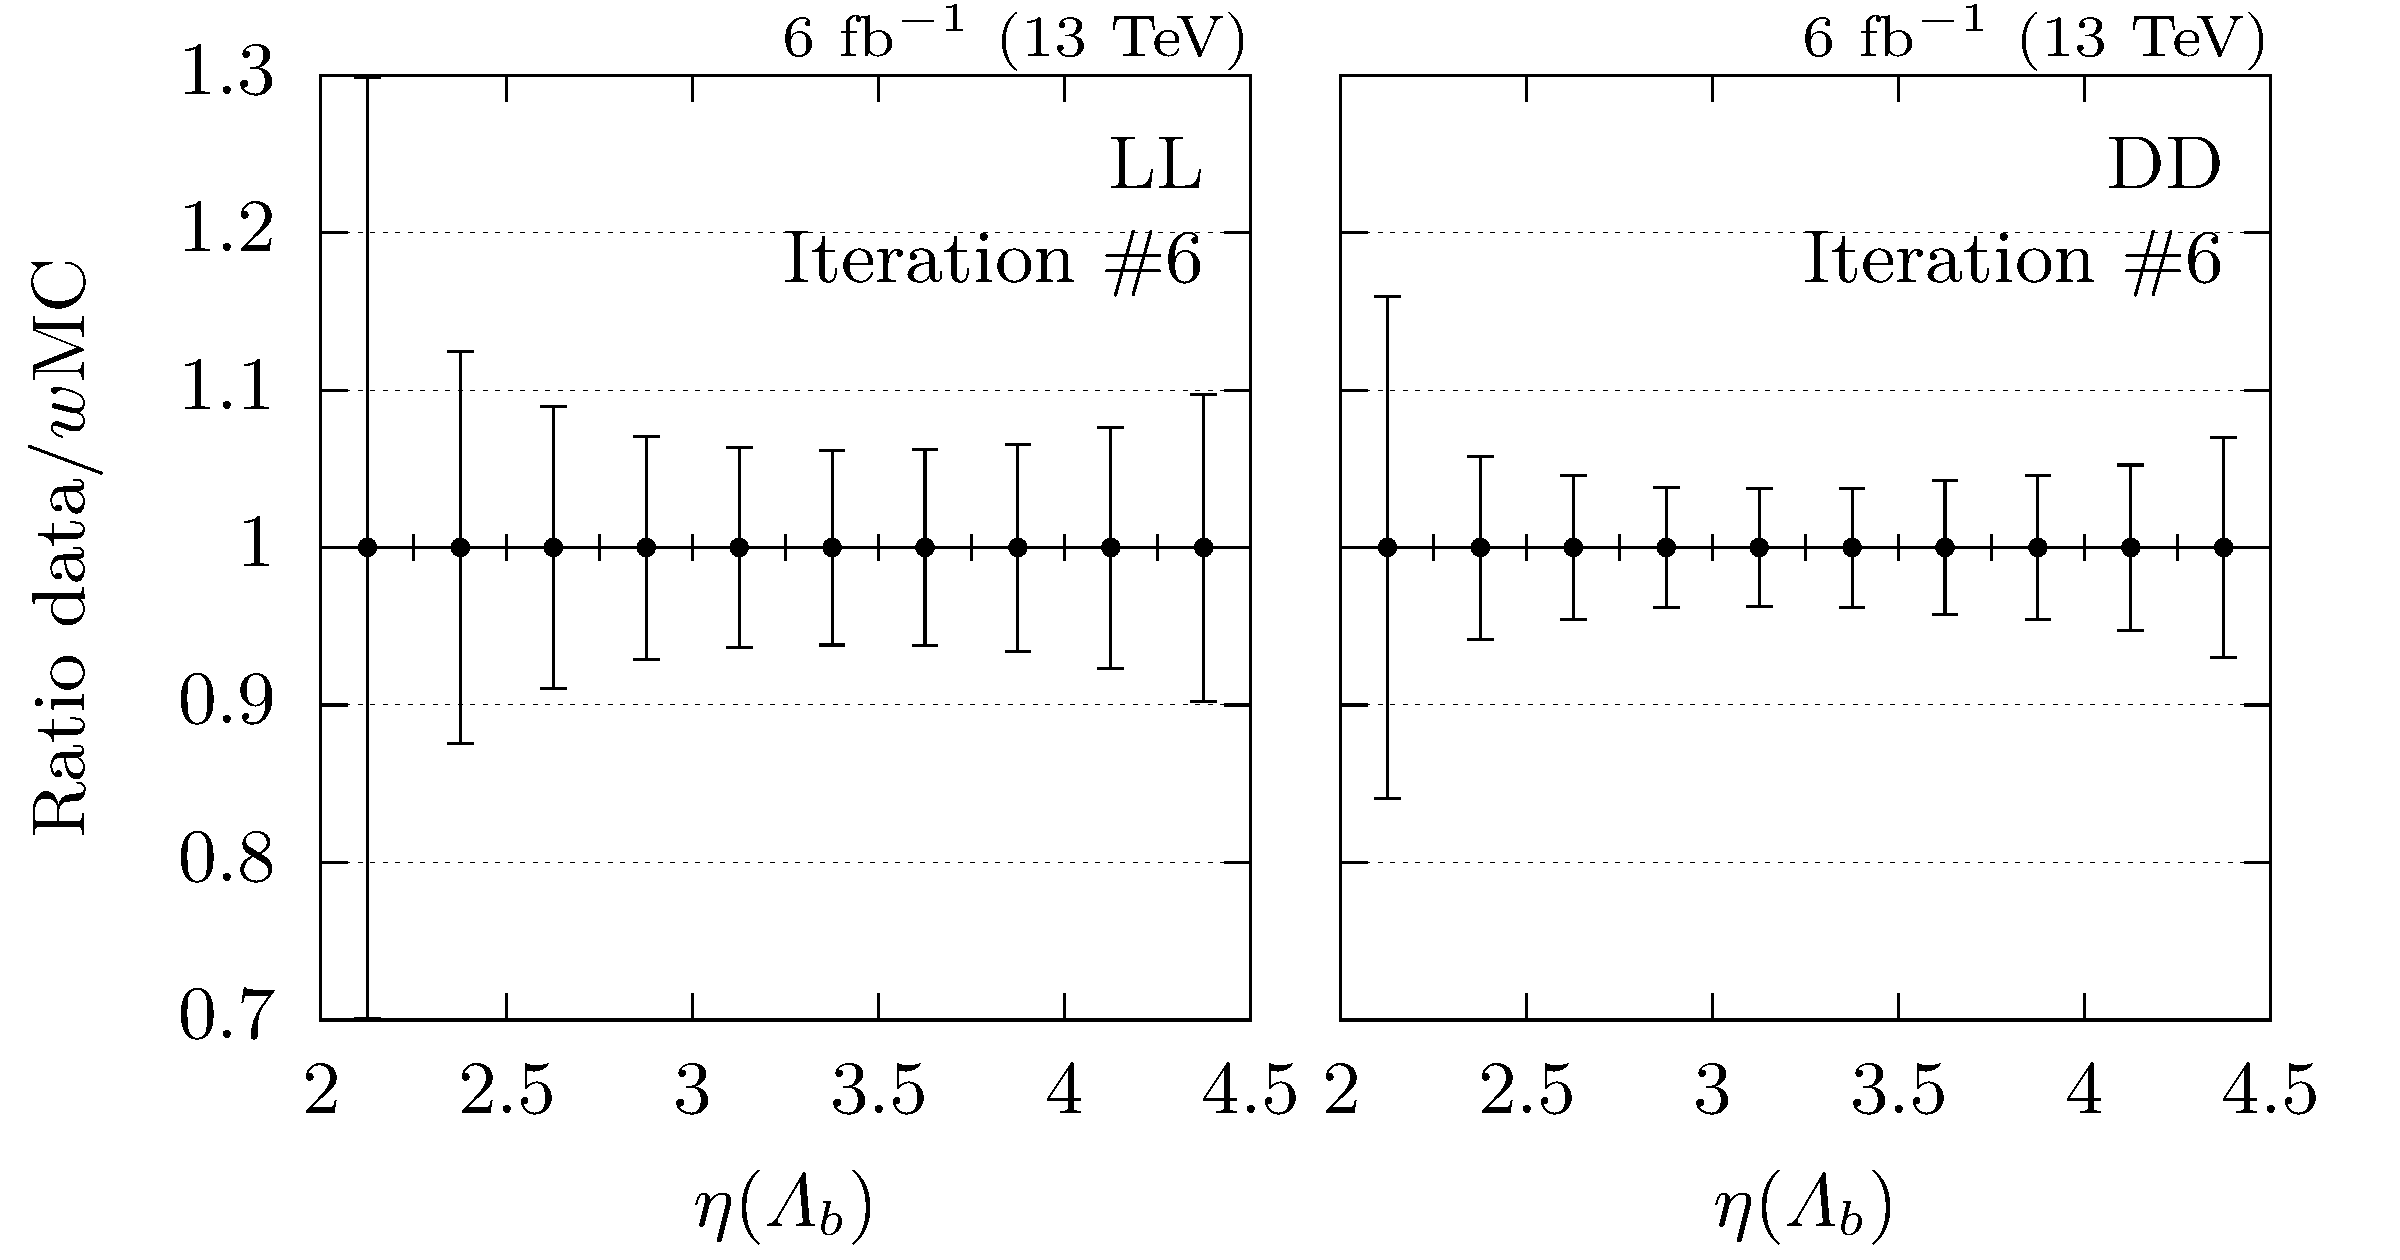
\includegraphics[scale=1.]{Lb2JpsiLz_weighting/hratio_eta_final.png}
%    \caption{Ratio of recorded data and weighted MC simulated events after six successive iterations in $\eta(\Lb)$ bins.}
%\end{figure}

%\begin{figure}[htbp]
%    \centering
%    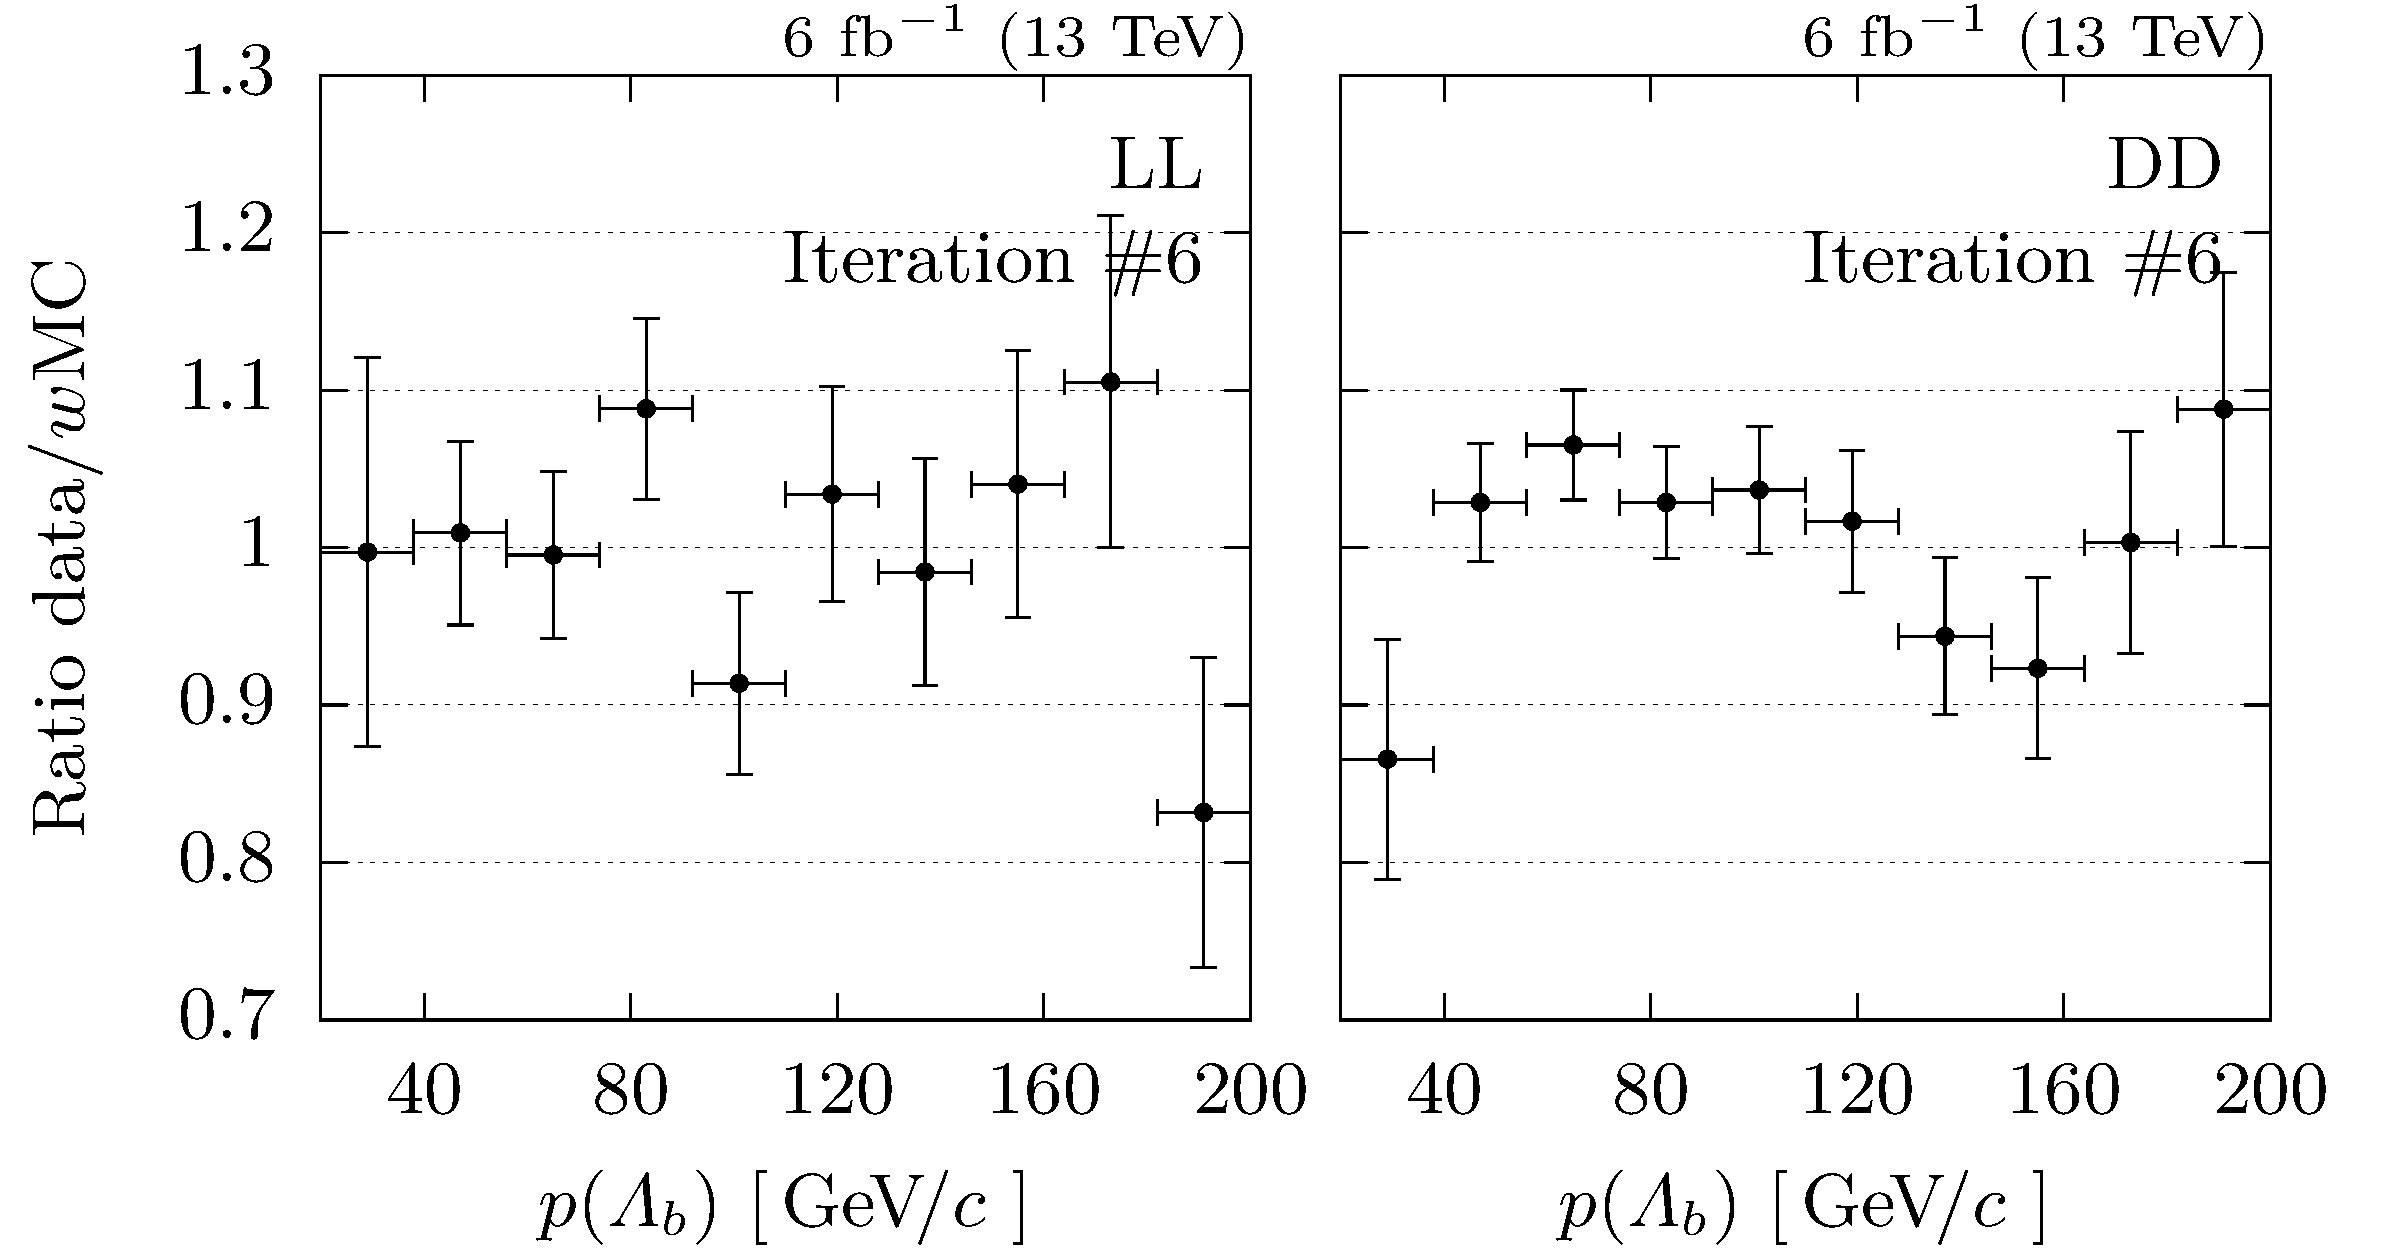
\includegraphics[scale=1.]{Lb2JpsiLz_weighting/hratio_p_final.png}
%    \caption{Ratio of recorded data and weighted MC simulated events after six successive iterations in $p(\Lb)$ bins.}
%\end{figure}

\begin{figure}[htbp]
    \centering
    \begin{subfigure}{\textwidth}
        \centering
        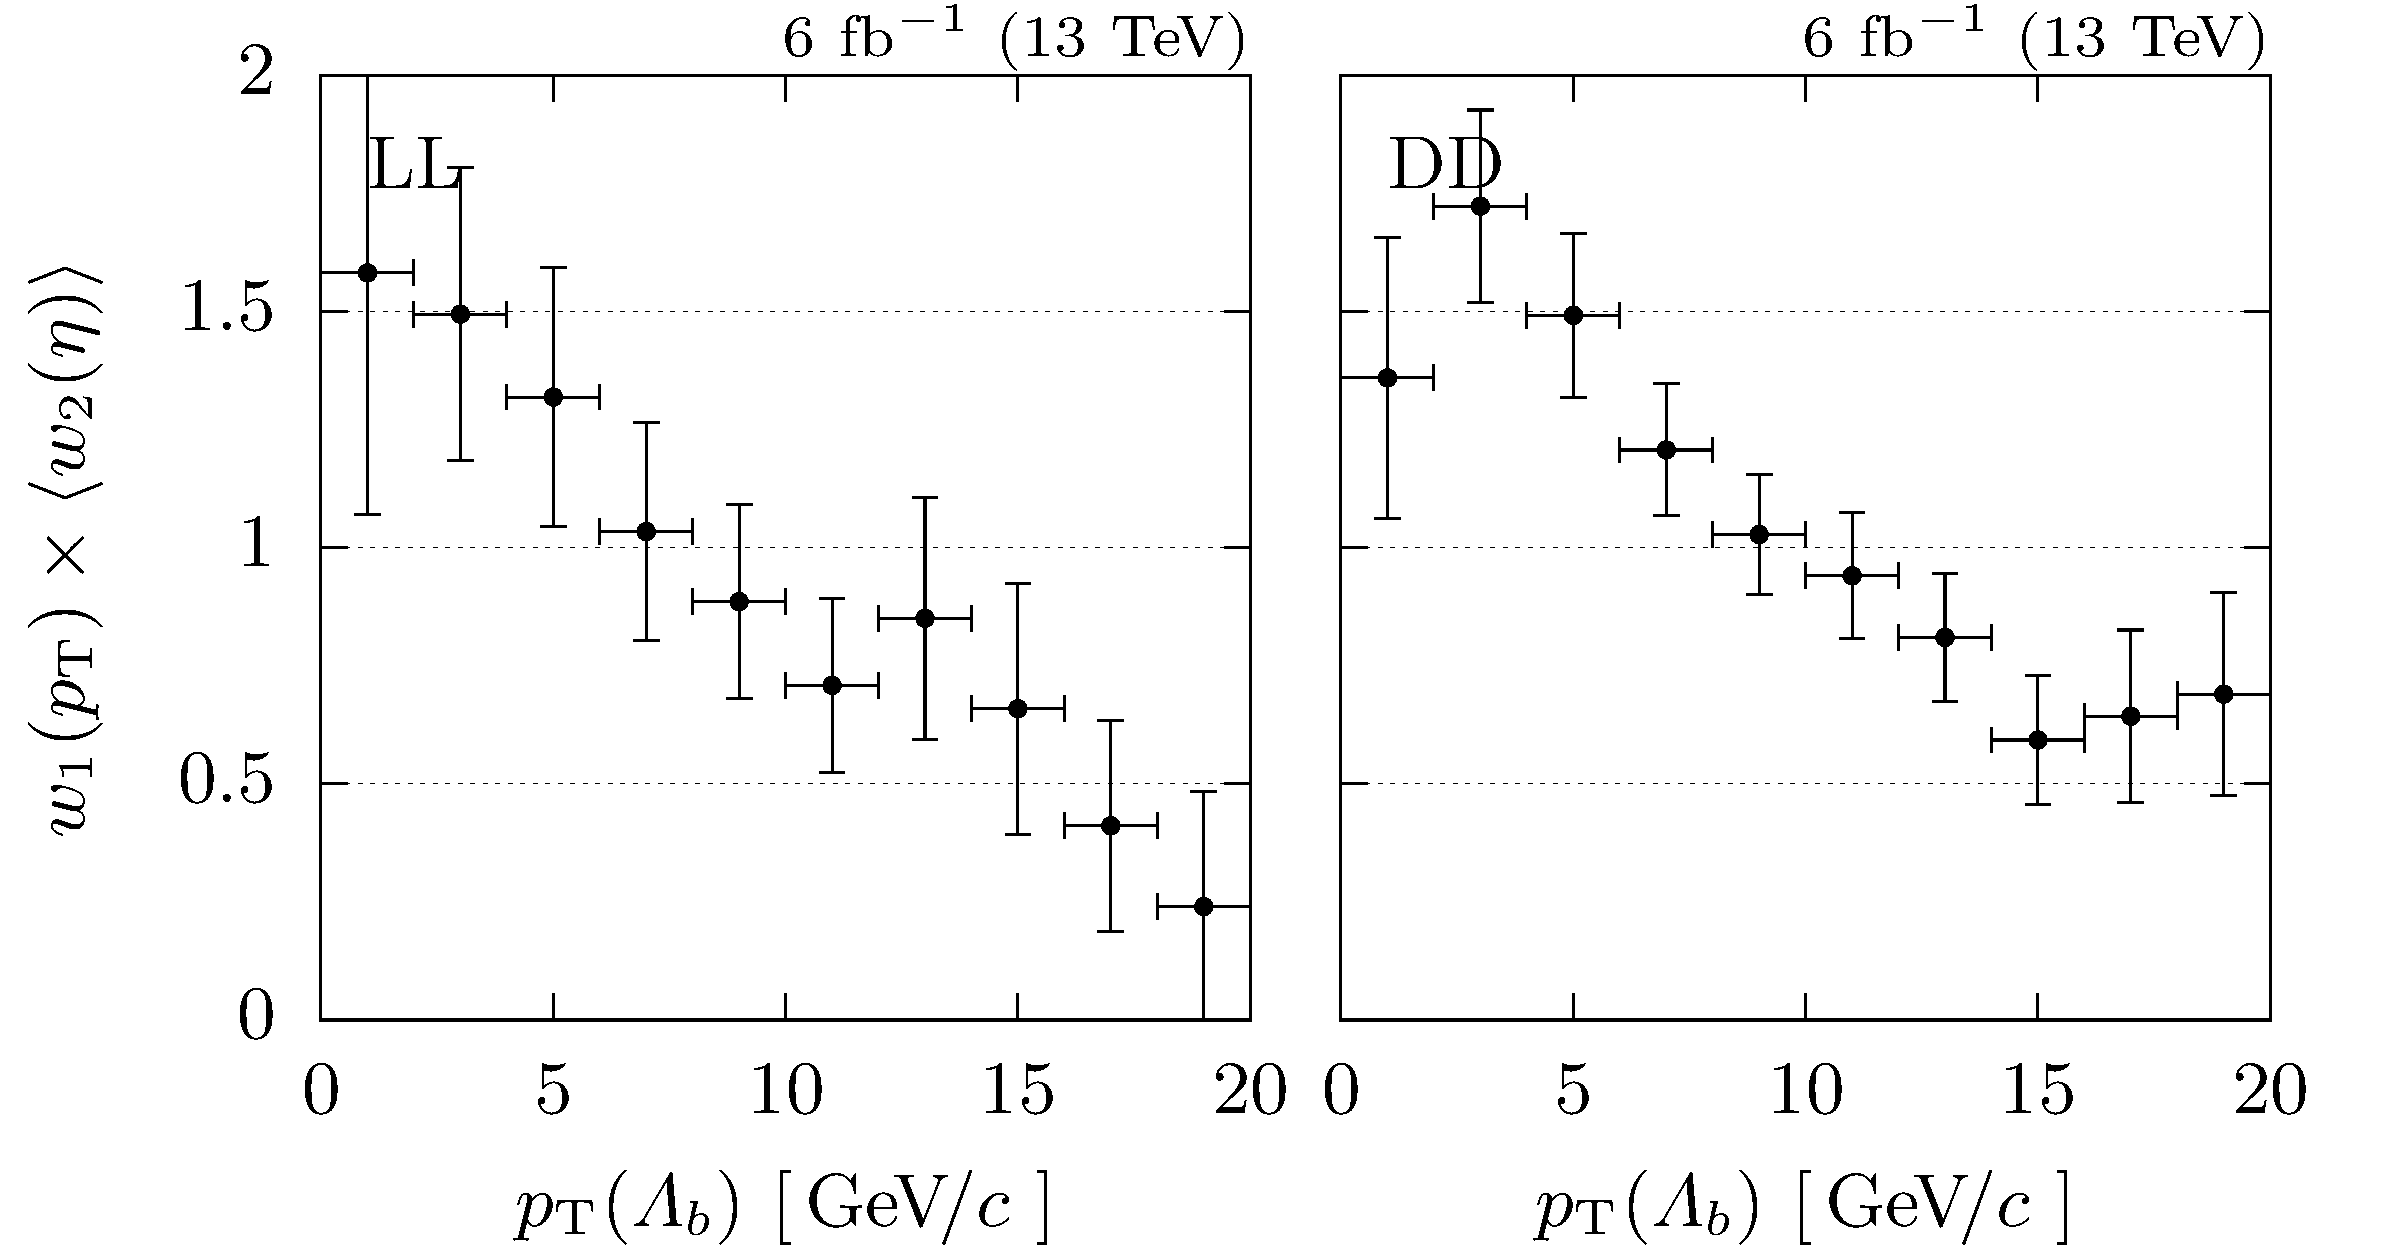
\includegraphics[scale=1.]{Lb2JpsiLz_weighting/avgw_prod_pT.png}
    \end{subfigure}
    \par\bigskip 
    \begin{subfigure}{\textwidth}
        \centering
        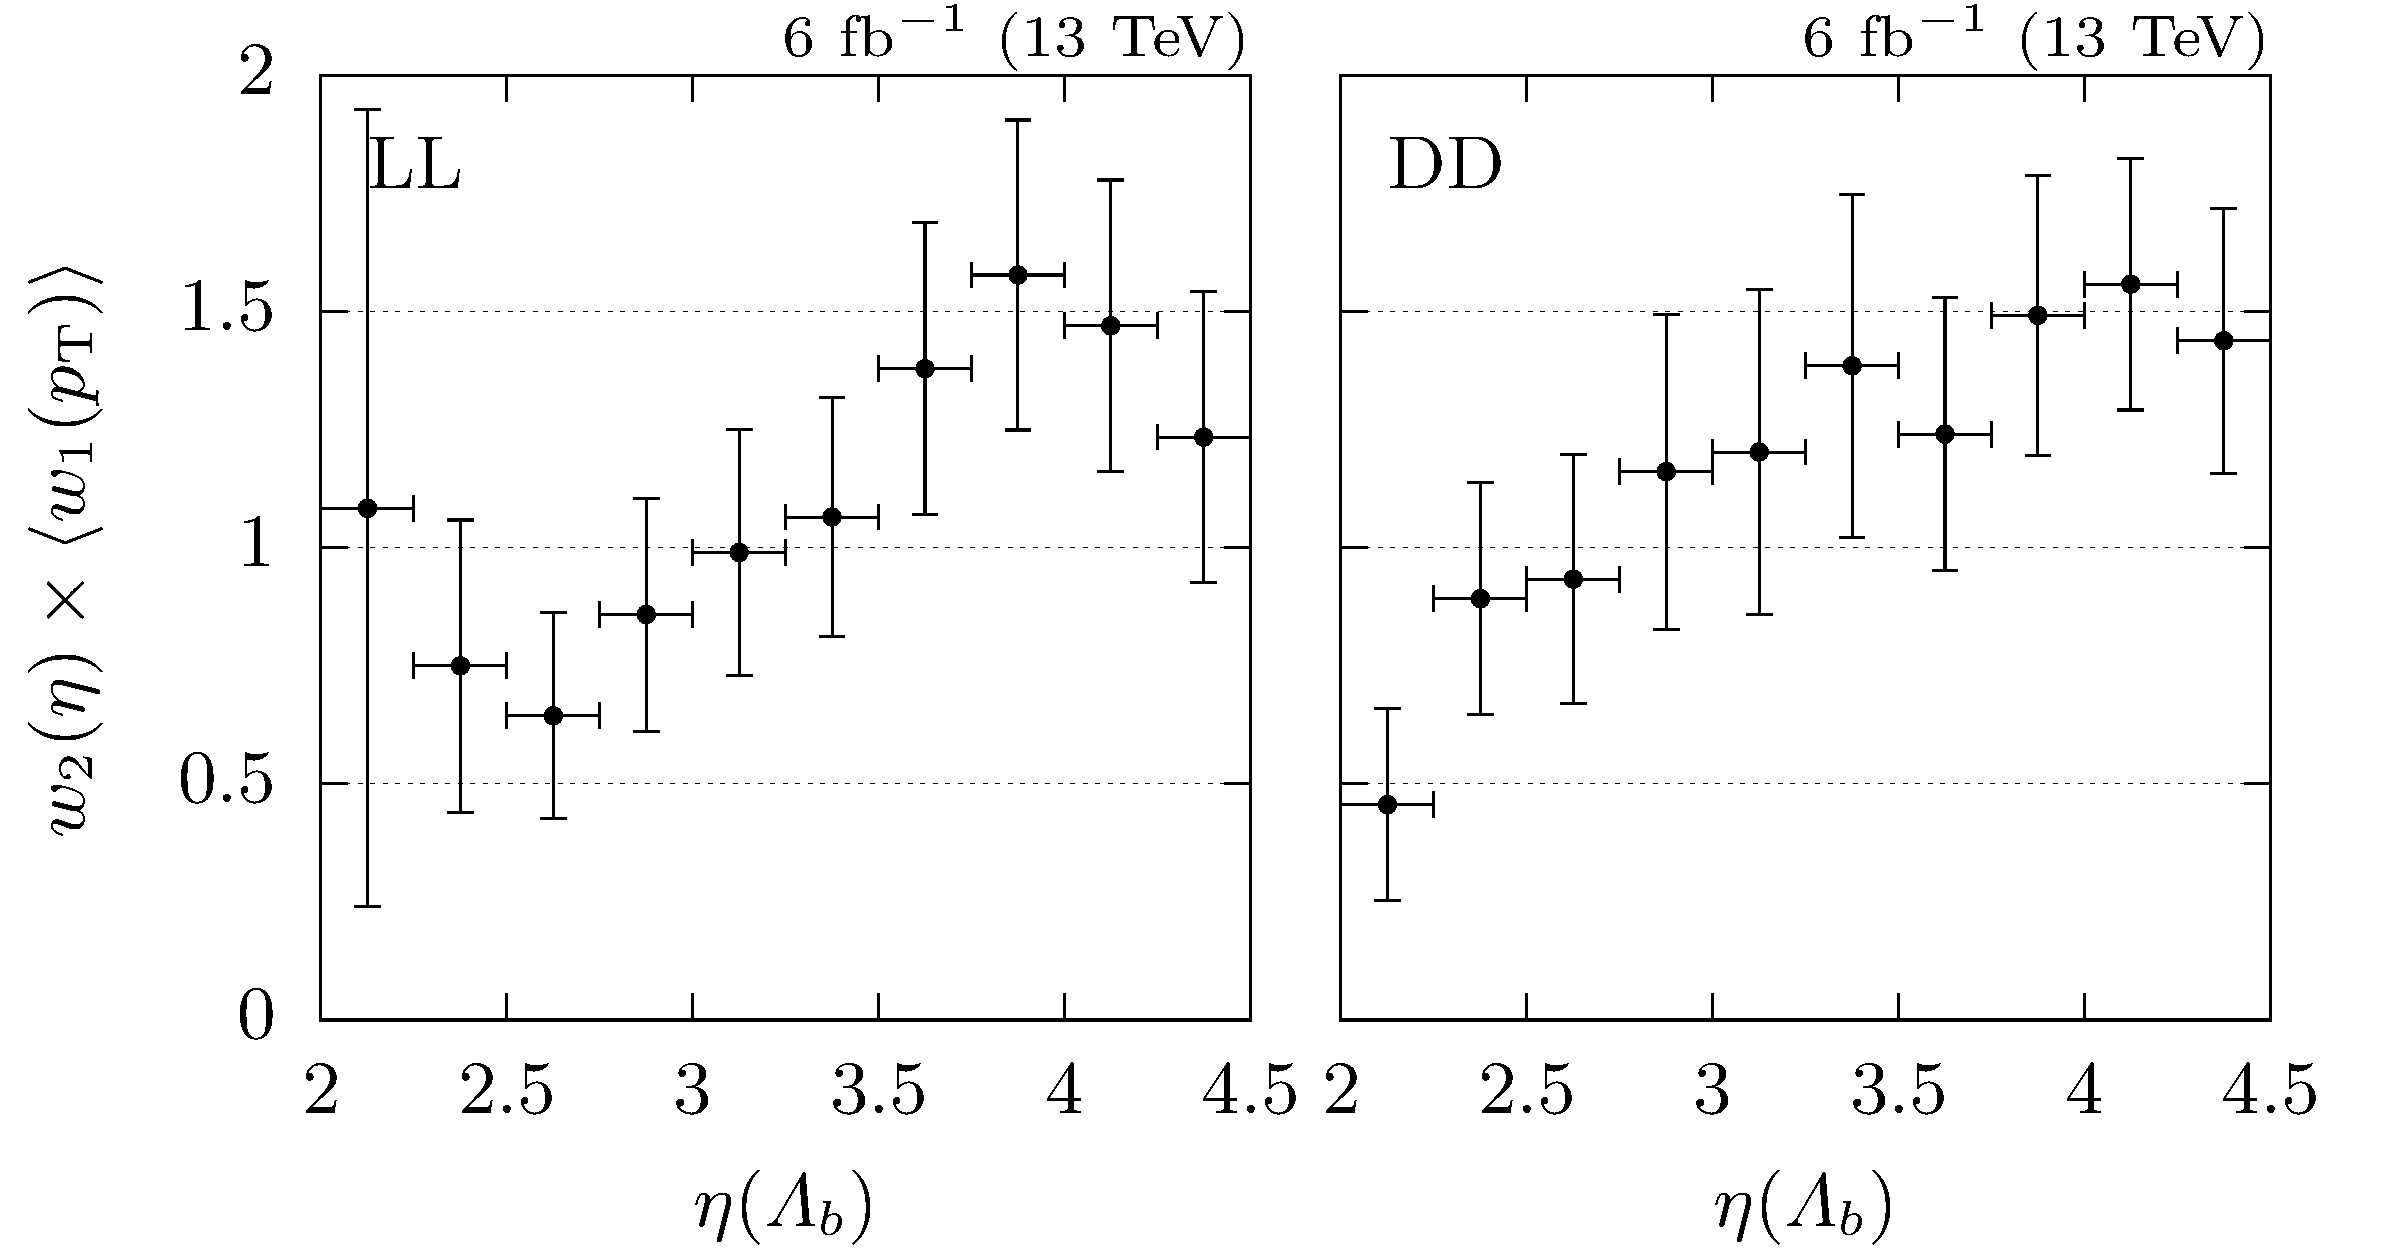
\includegraphics[scale=1.]{Lb2JpsiLz_weighting/avgw_prod_eta.png}
    \end{subfigure}
    \caption{Product of $w_1(\pt)$ and the mean of $w_2(\eta)$ (top) and vice versa (bottom) for \gls{LL} (left) and \gls{DD} (right) tracks.}
    \label{fig:LbToJpsiLz_avgw_prod}
\end{figure}

\begin{table}[htbp]
    \centering
    \caption{$p$-values w.r.t.\ the hypotheses $w_1(\pt)=1$ and $w_2(\eta)=1$ after six successive iterations, as well as the change of the $p$-value for $r(p)=1$, where $r(p)$ is the (binned) ratio of the three-momentum magnitude distribution of recorded data and simulated events, during the iterations.}
    \label{tab:LbToJpsiLz_pvalues}
    \begin{tabular}{ccc}
        \toprule
        & \gls{LL} & \gls{DD} \\
        \midrule
        $w_1(\pt)$ & $3\,\%$ & $0\,\%$ \\
        $w_2(\eta)$ & $71\,\%$ & $59\,\%$ \\
        \midrule
        $r(p)$ & $2\,\% \mapsto 53\,\%$ & $0\,\% \mapsto 24\,\%$ \\
        \bottomrule
    \end{tabular}
\end{table}

It is worthwhile to mention that the final weights do differ from the initial ratio of recorded and yet unweighted simulated events due to the correlation between \pt and $\eta$.
It is the product of $w_1(\pt)$ and $w_2(\eta)$ that will eventually reproduce the initially observed ratios, not the marginal distributions themself.
A visualization of this is given in the Fig.~\ref{fig:LbToJpsiLz_avgw_prod} that shows the product of $w_1(\pt)$ and the mean of $w_2(\eta)$ and vice versa for \gls{LL} and \gls{DD} tracks.

%\begin{figure}[htbp]
%    \centering
%    \begin{subfigure}{\textwidth}
%        \centering
%        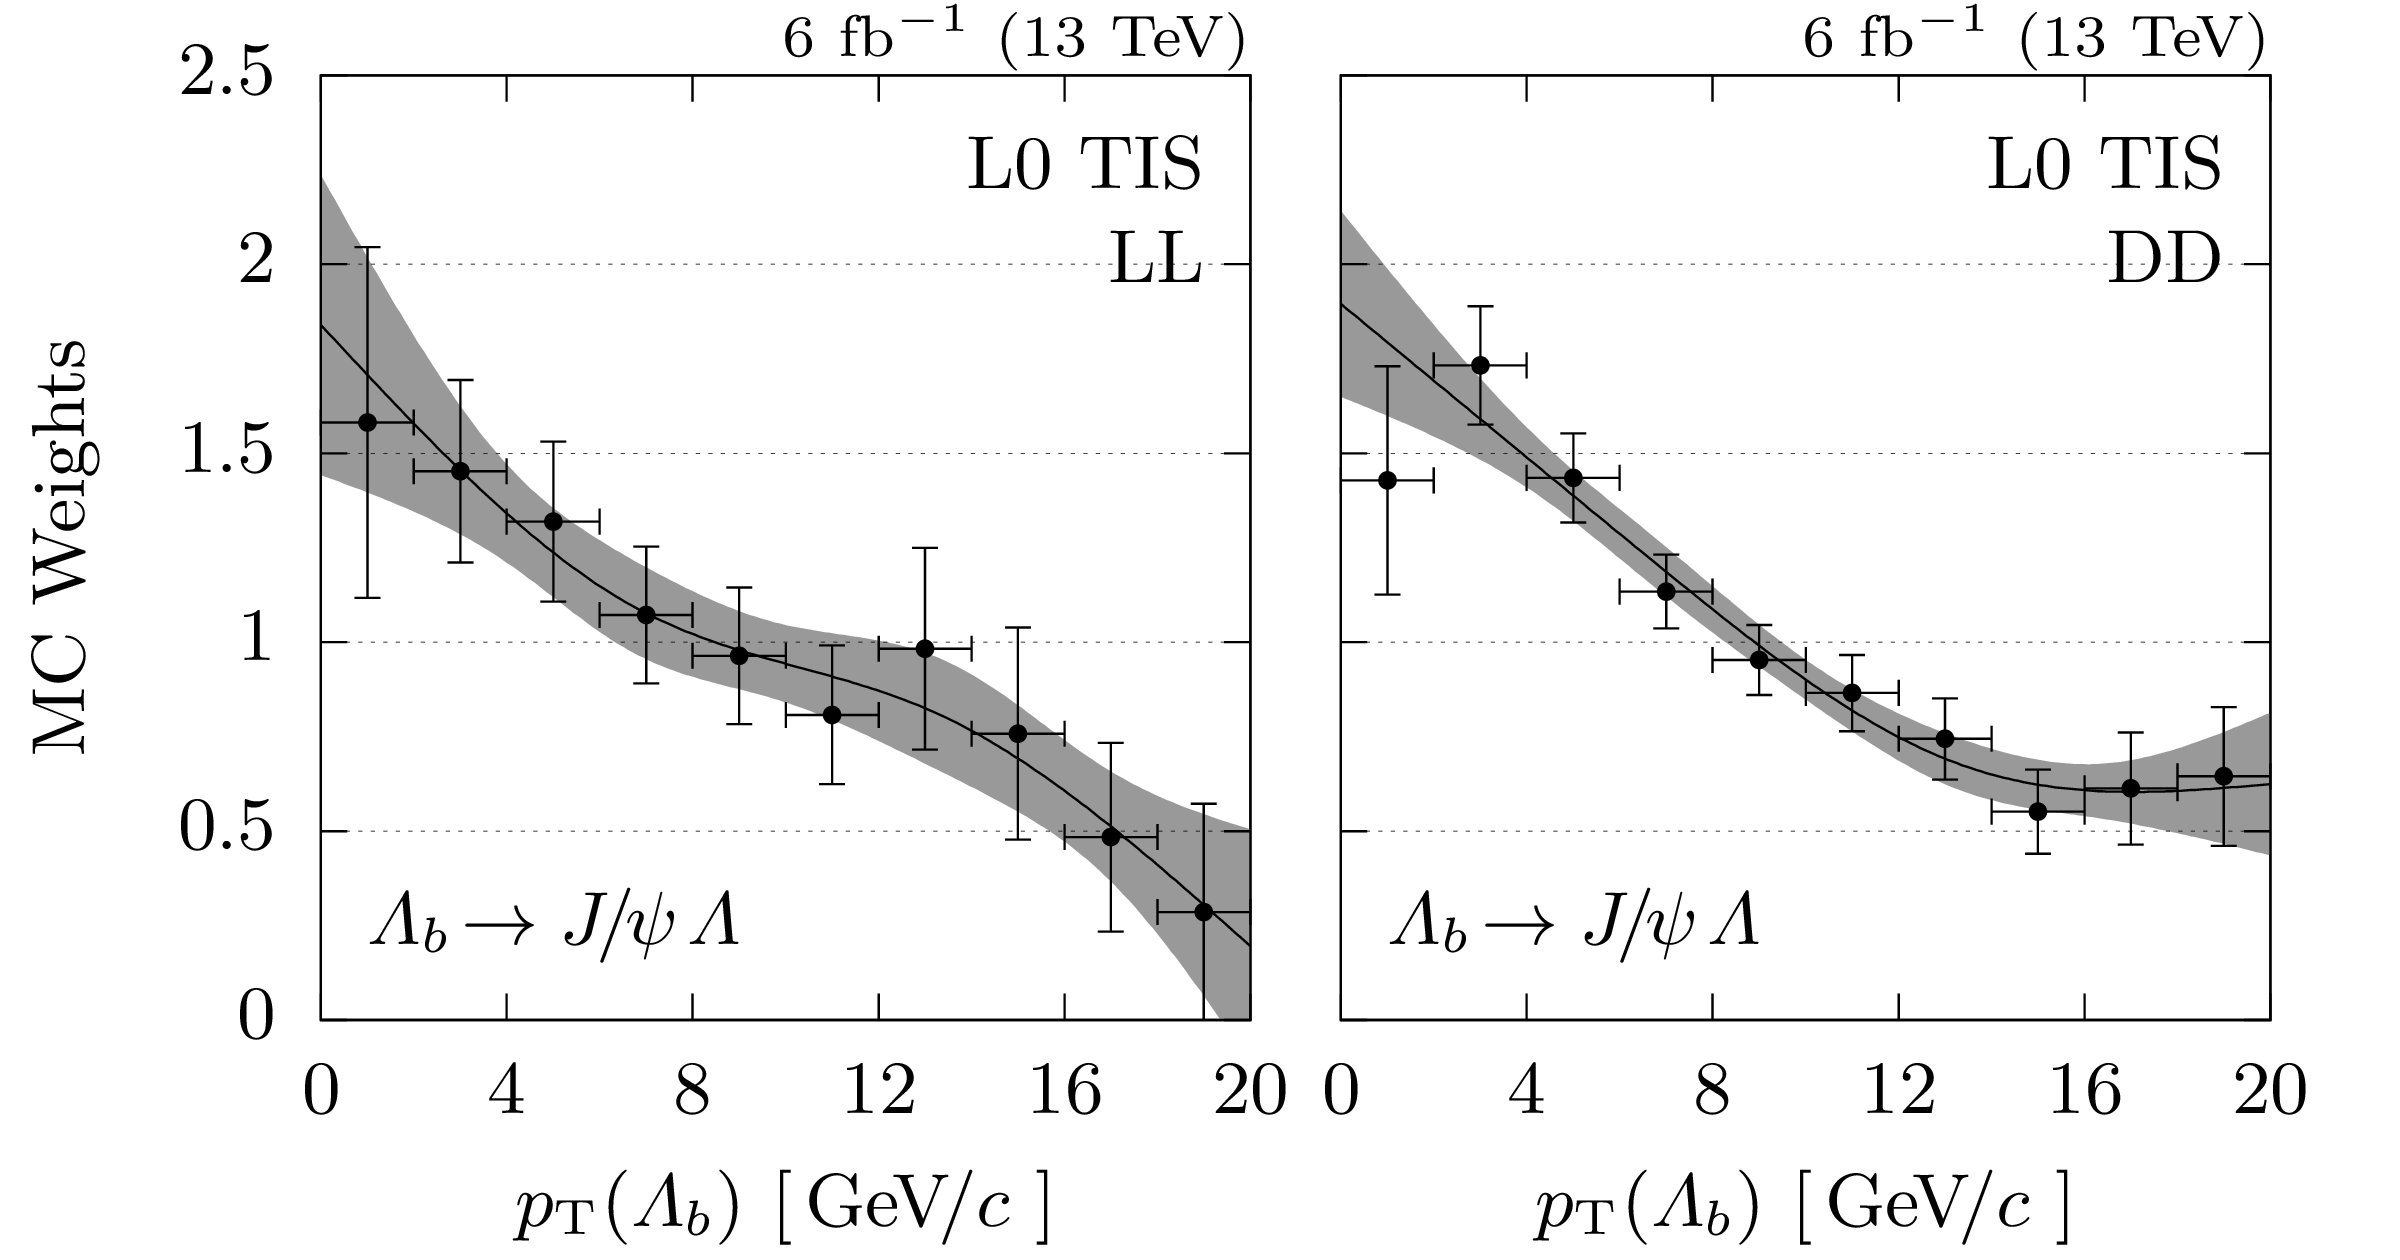
\includegraphics[scale=1.]{Lb2JpsiLz_weighting/weights_pT.png}
%    \end{subfigure}
%    \par\bigskip 
%    \begin{subfigure}{\textwidth}
%        \centering
%        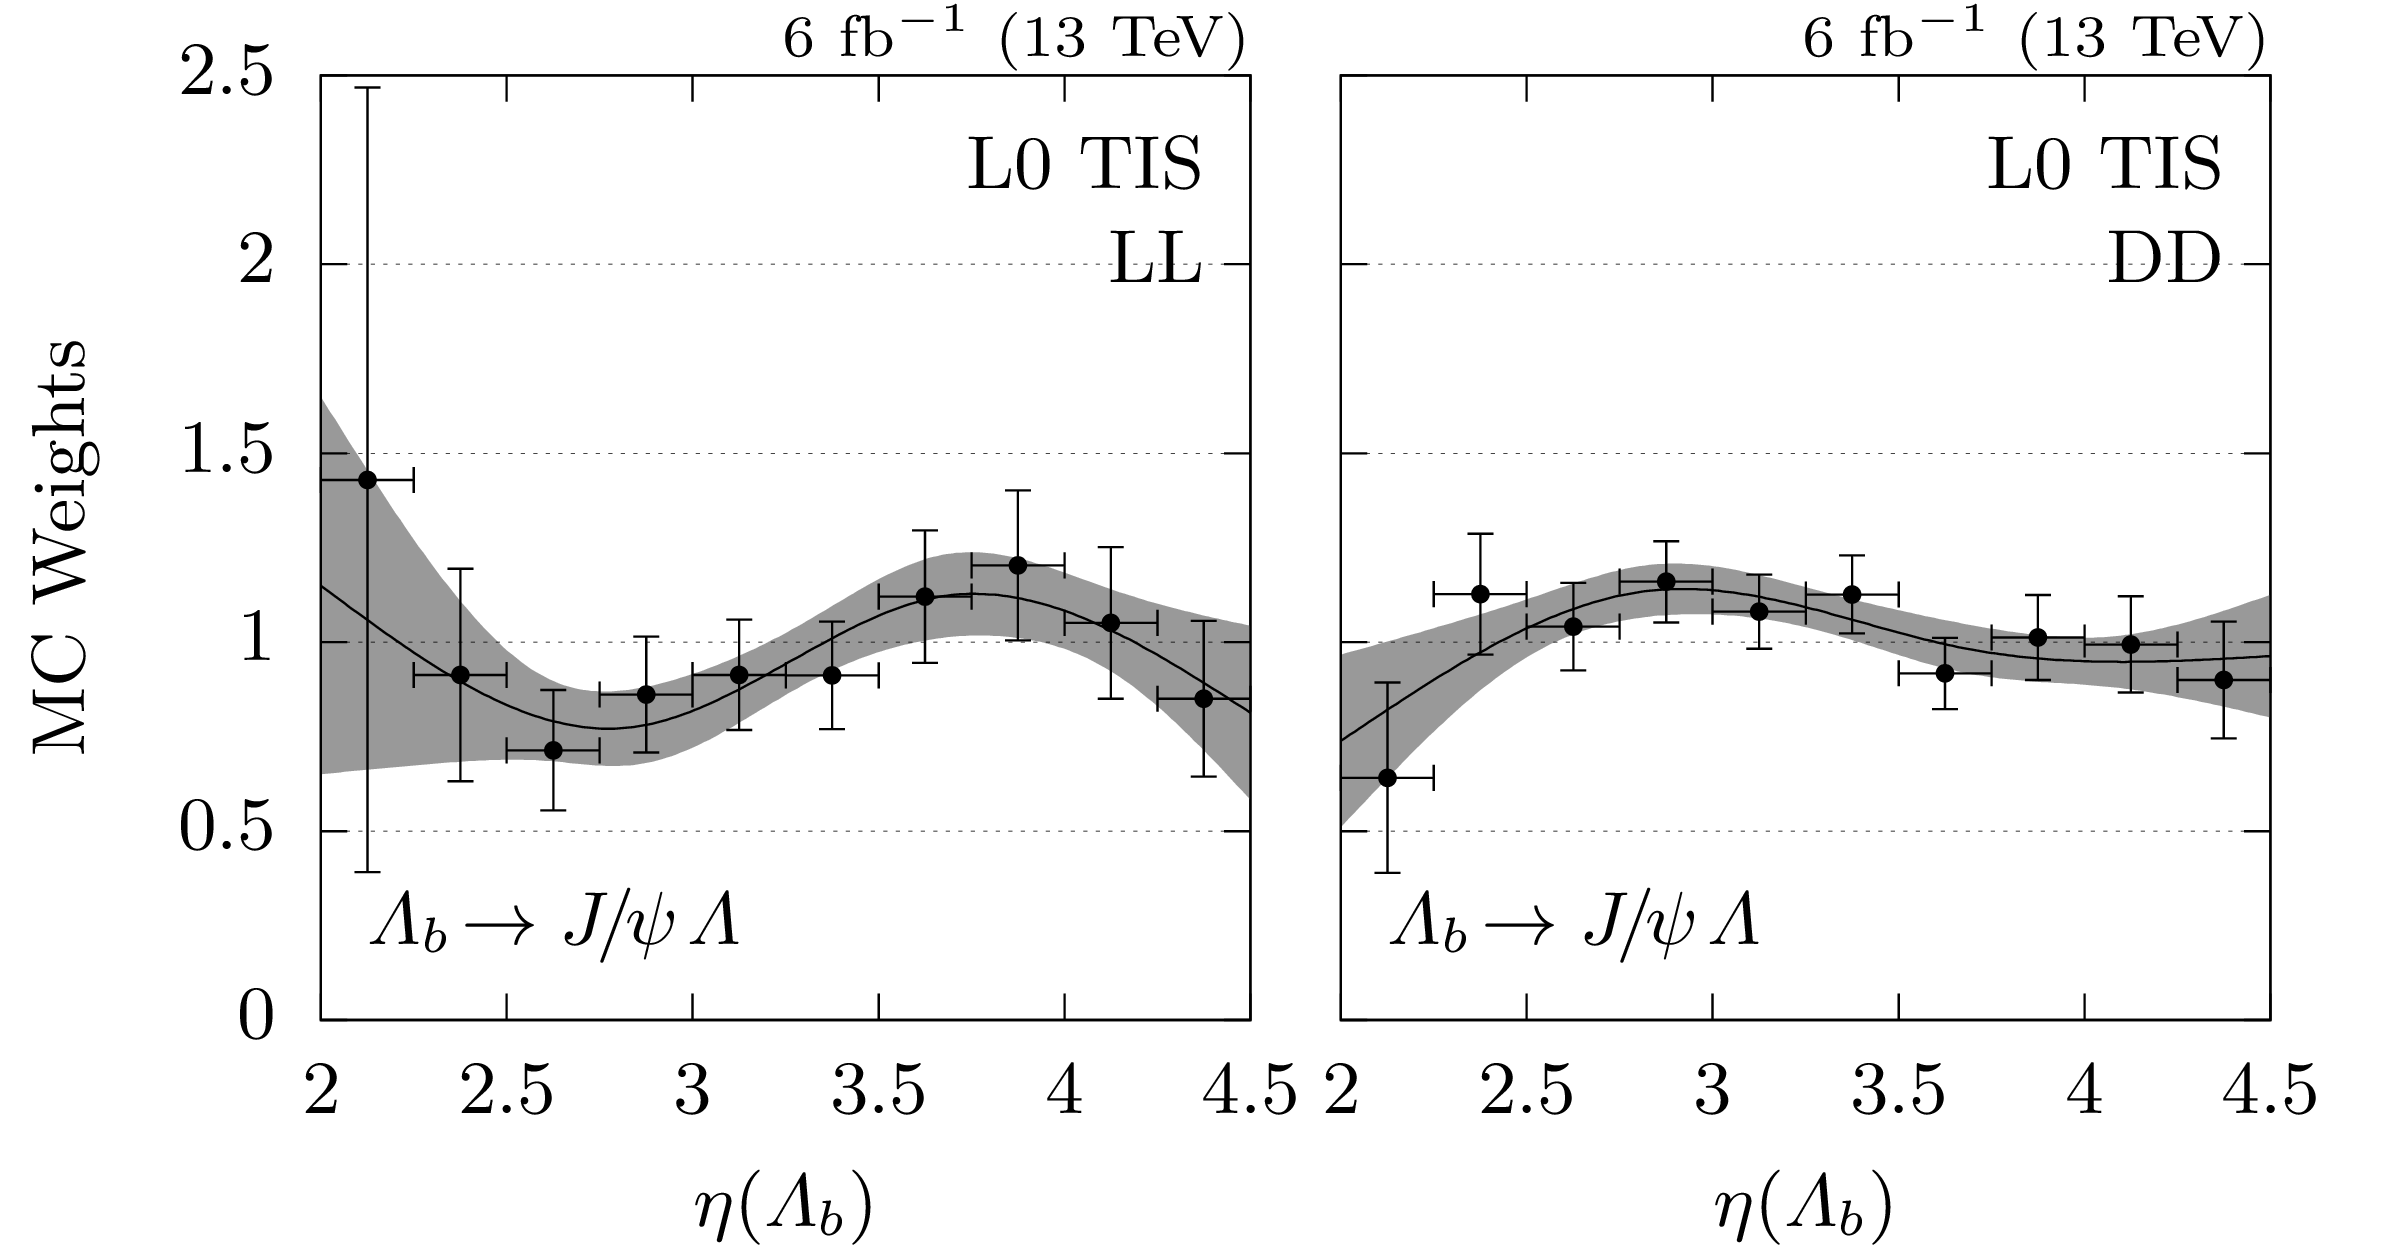
\includegraphics[scale=1.]{Lb2JpsiLz_weighting/weights_eta.png}
%    \end{subfigure}
%    \caption{Weights $w_1(\pt)$ (top) and $w_2(\eta)$ (bottom) for \gls{LL} (left) and \gls{DD} (right) tracks, as well as four independent equidistant (natural) cubic spline fits, each with four \gls{dof}.}
%    \label{fig:LbToJpsiLz_weights}
%\end{figure}

A priori, the distribution of weights cannot expected to be smooth, since each bin is corrected individually.
However, due to correlations, each \pt bin is linked to an entire set of $\eta$ bins and vice versa.
A correction of one bin will therefore also influence the weights of neighboring bins, hence a smoothing algorithm can be applied to reduce \gls{dof} and compensate uncertainties partially of each bin.

The separate weighting of \gls{LL} and \gls{DD} tracks was chosen, because doing so takes different selection criteria and heterogeneous sample sizes trivially into account.
However, separate weighting is not physically motivated, since the genuine \pt and $\eta$ distributions of $\Lb$ particles should be the same and independent of a specific decay mode or the track type of a \mbox{(grand-)daughter}.
In order to include this physical constraint back in, smoothing by fitting (natural) equidistant cubic splines with four \gls{dof} (\cf{}~Appx.~\ref{chap:csplines}) is performed separately for $w_1(\pt)$ and $w_2(\eta)$, but simultaneously for the different track types.
The resulting fits are shown in Fig.~\ref{fig:LbToJpsiLz_weights_simfit} together with the distributions of $w_1(\pt)$ and $w_2(\eta)$ and show an unphysical discrepancy between \gls{LL} and \gls{DD} tracks for $w_2(\eta)$.

%An equidistant (natural) cubic spline fit with four \gls{dof} is used to smooth $w_1(\pt)$ and $w_2(\eta)$ for both track types, separately.
%The result is shown in Fig.~\ref{fig:LbToJpsiLz_weights}.
%The discrepancy between \gls{LL} and \gls{DD} tracks for $w_2(\eta)$ is not physical since the true \pt and $\eta$ distributions of all $\Lb$ particles should be the same and independent of a specific decay mode or the track type of a (grand-)daughter.
%
\begin{figure}[htbp]
    \begin{subfigure}{\textwidth}
        \centering
        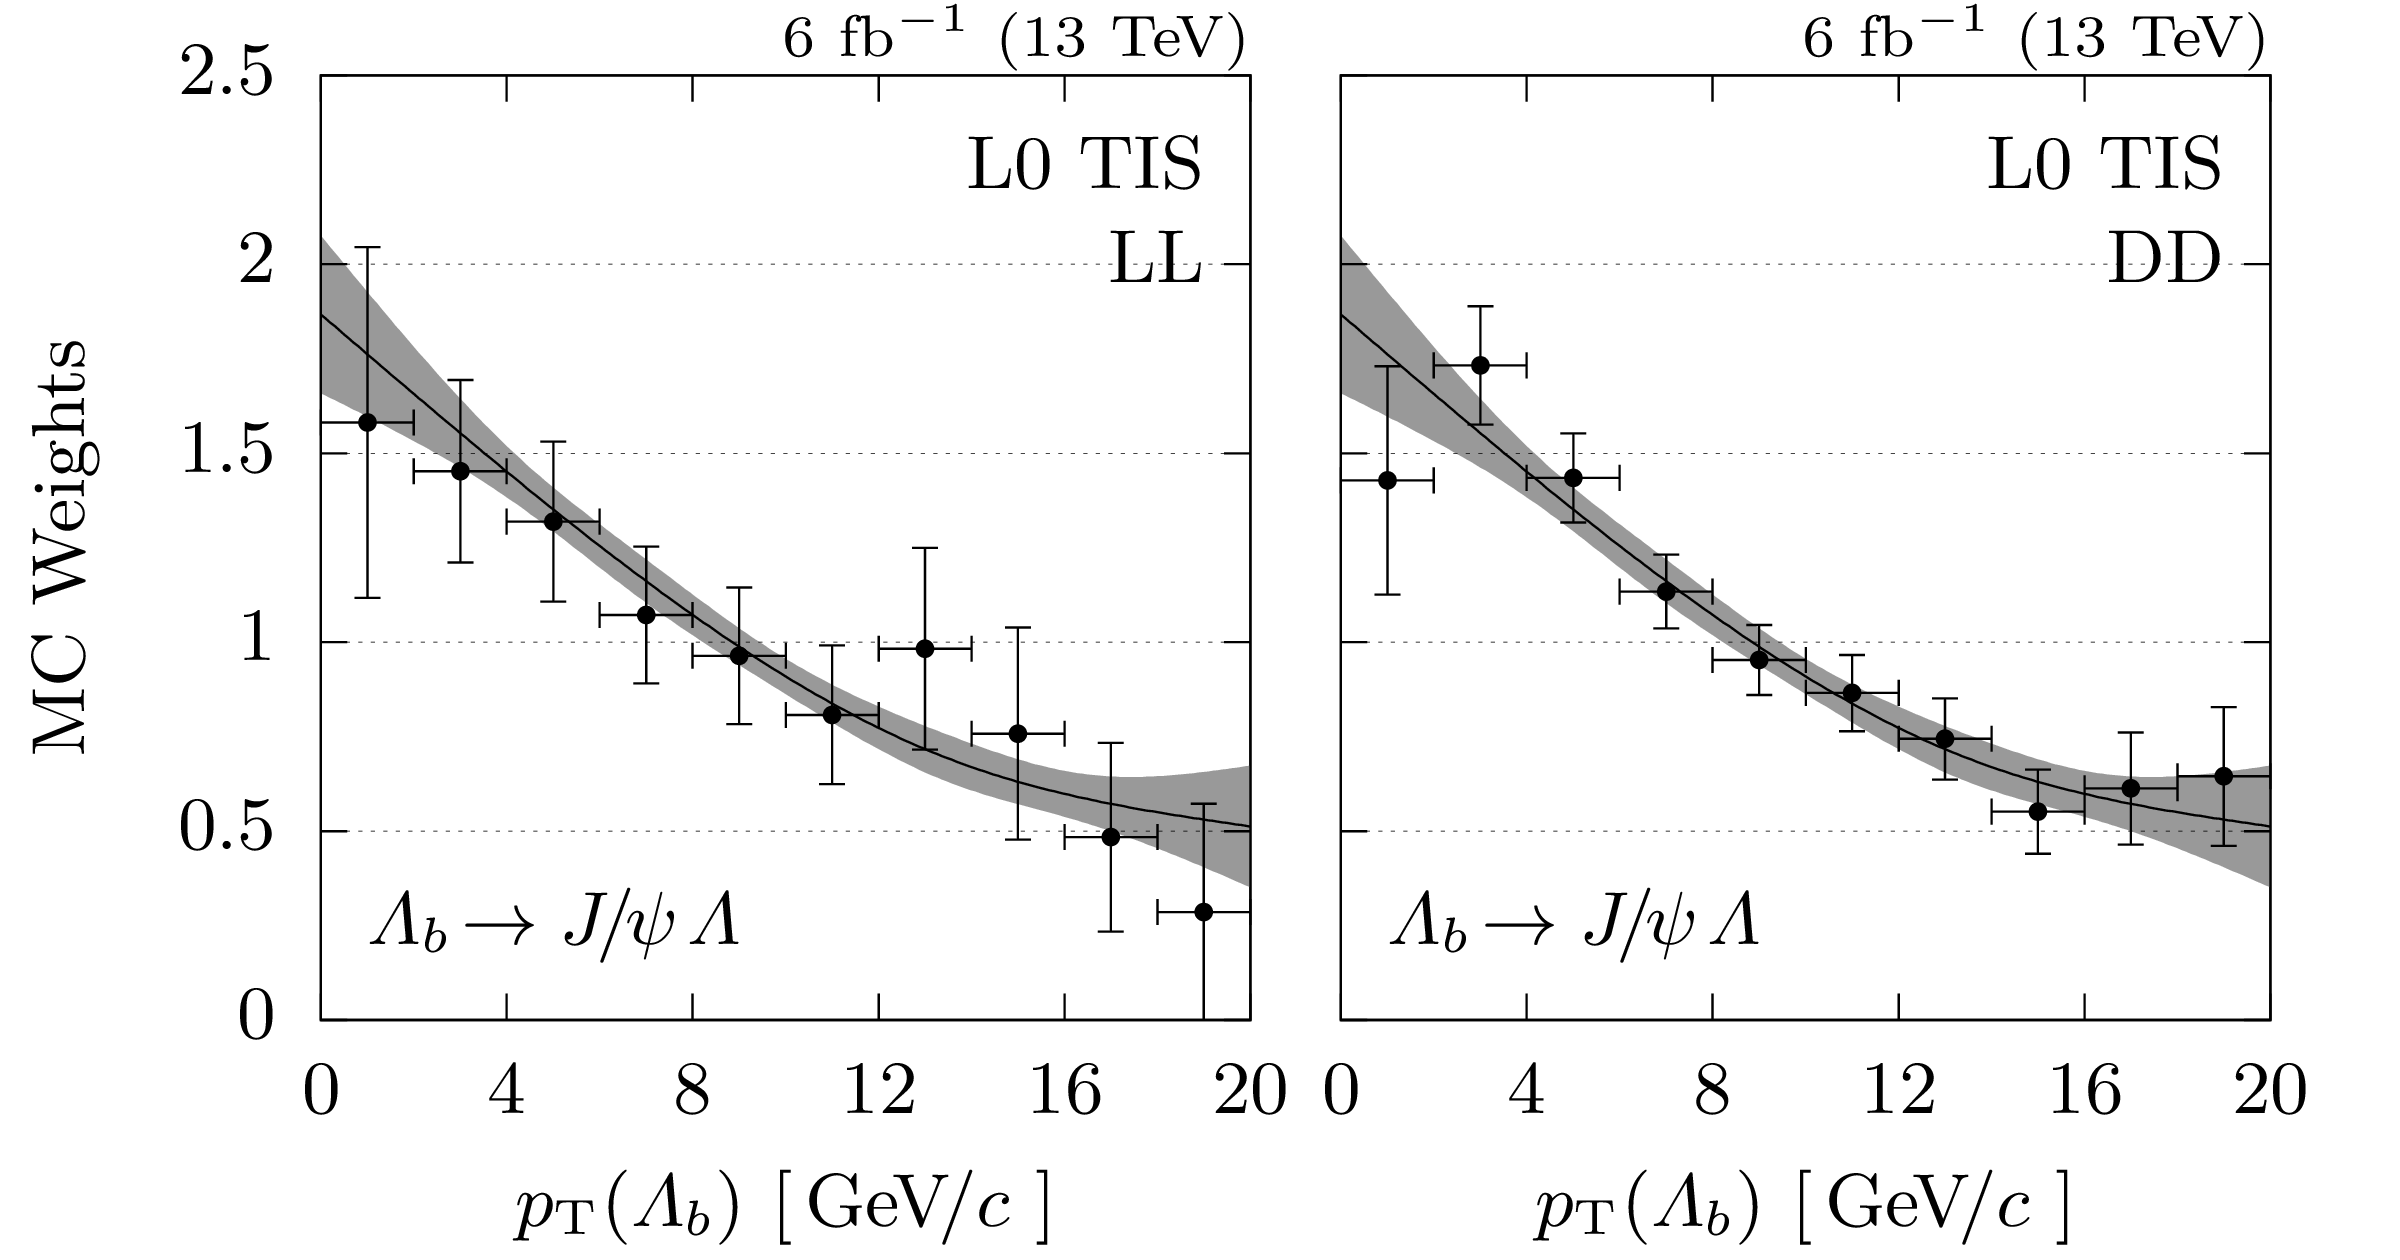
\includegraphics[scale=1.]{Lb2JpsiLz_weighting/weights_pT_simfit.png}
    \end{subfigure}
    \par\bigskip 
    \begin{subfigure}{\textwidth}
        \centering
        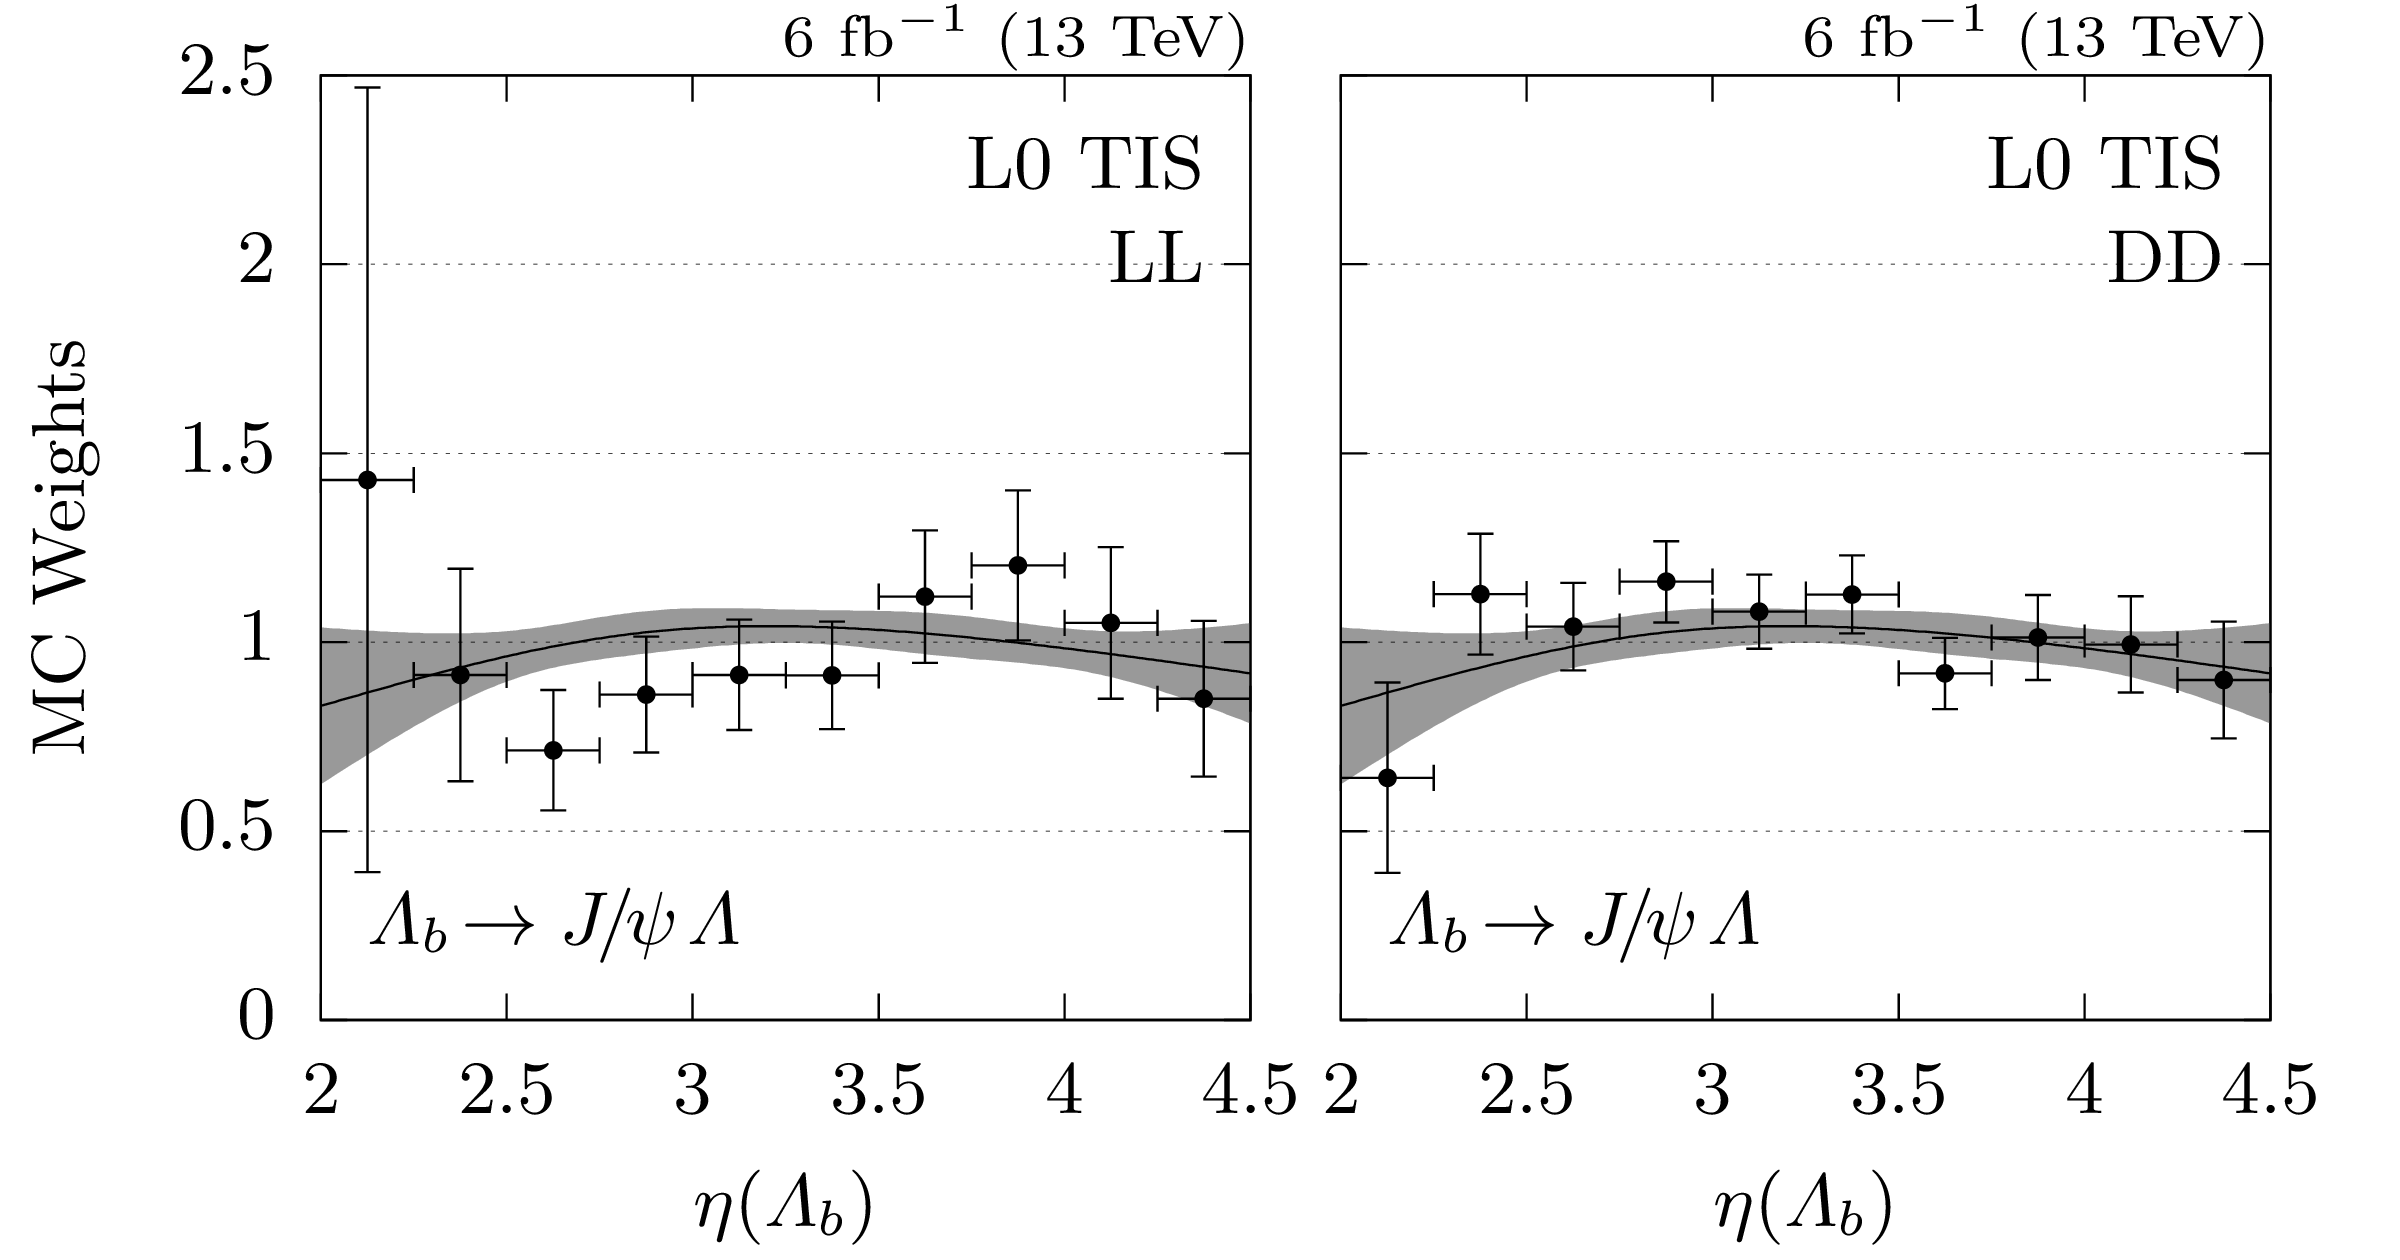
\includegraphics[scale=1.]{Lb2JpsiLz_weighting/weights_eta_simfit.png}
    \end{subfigure}
    \caption{Weights $w_1(\pt)$ (top) and $w_2(\eta)$ (bottom) for \gls{LL} (left) and \gls{DD} (right) tracks, as well as two equidistant (natural) cubic spline fits, each with four \gls{dof}. The distributions for \gls{LL} and \gls{DD} tracks are fitted simultaneously.}
    \label{fig:LbToJpsiLz_weights_simfit}
\end{figure}

\begin{figure}[htbp]
    \begin{subfigure}{\textwidth}
        \centering
        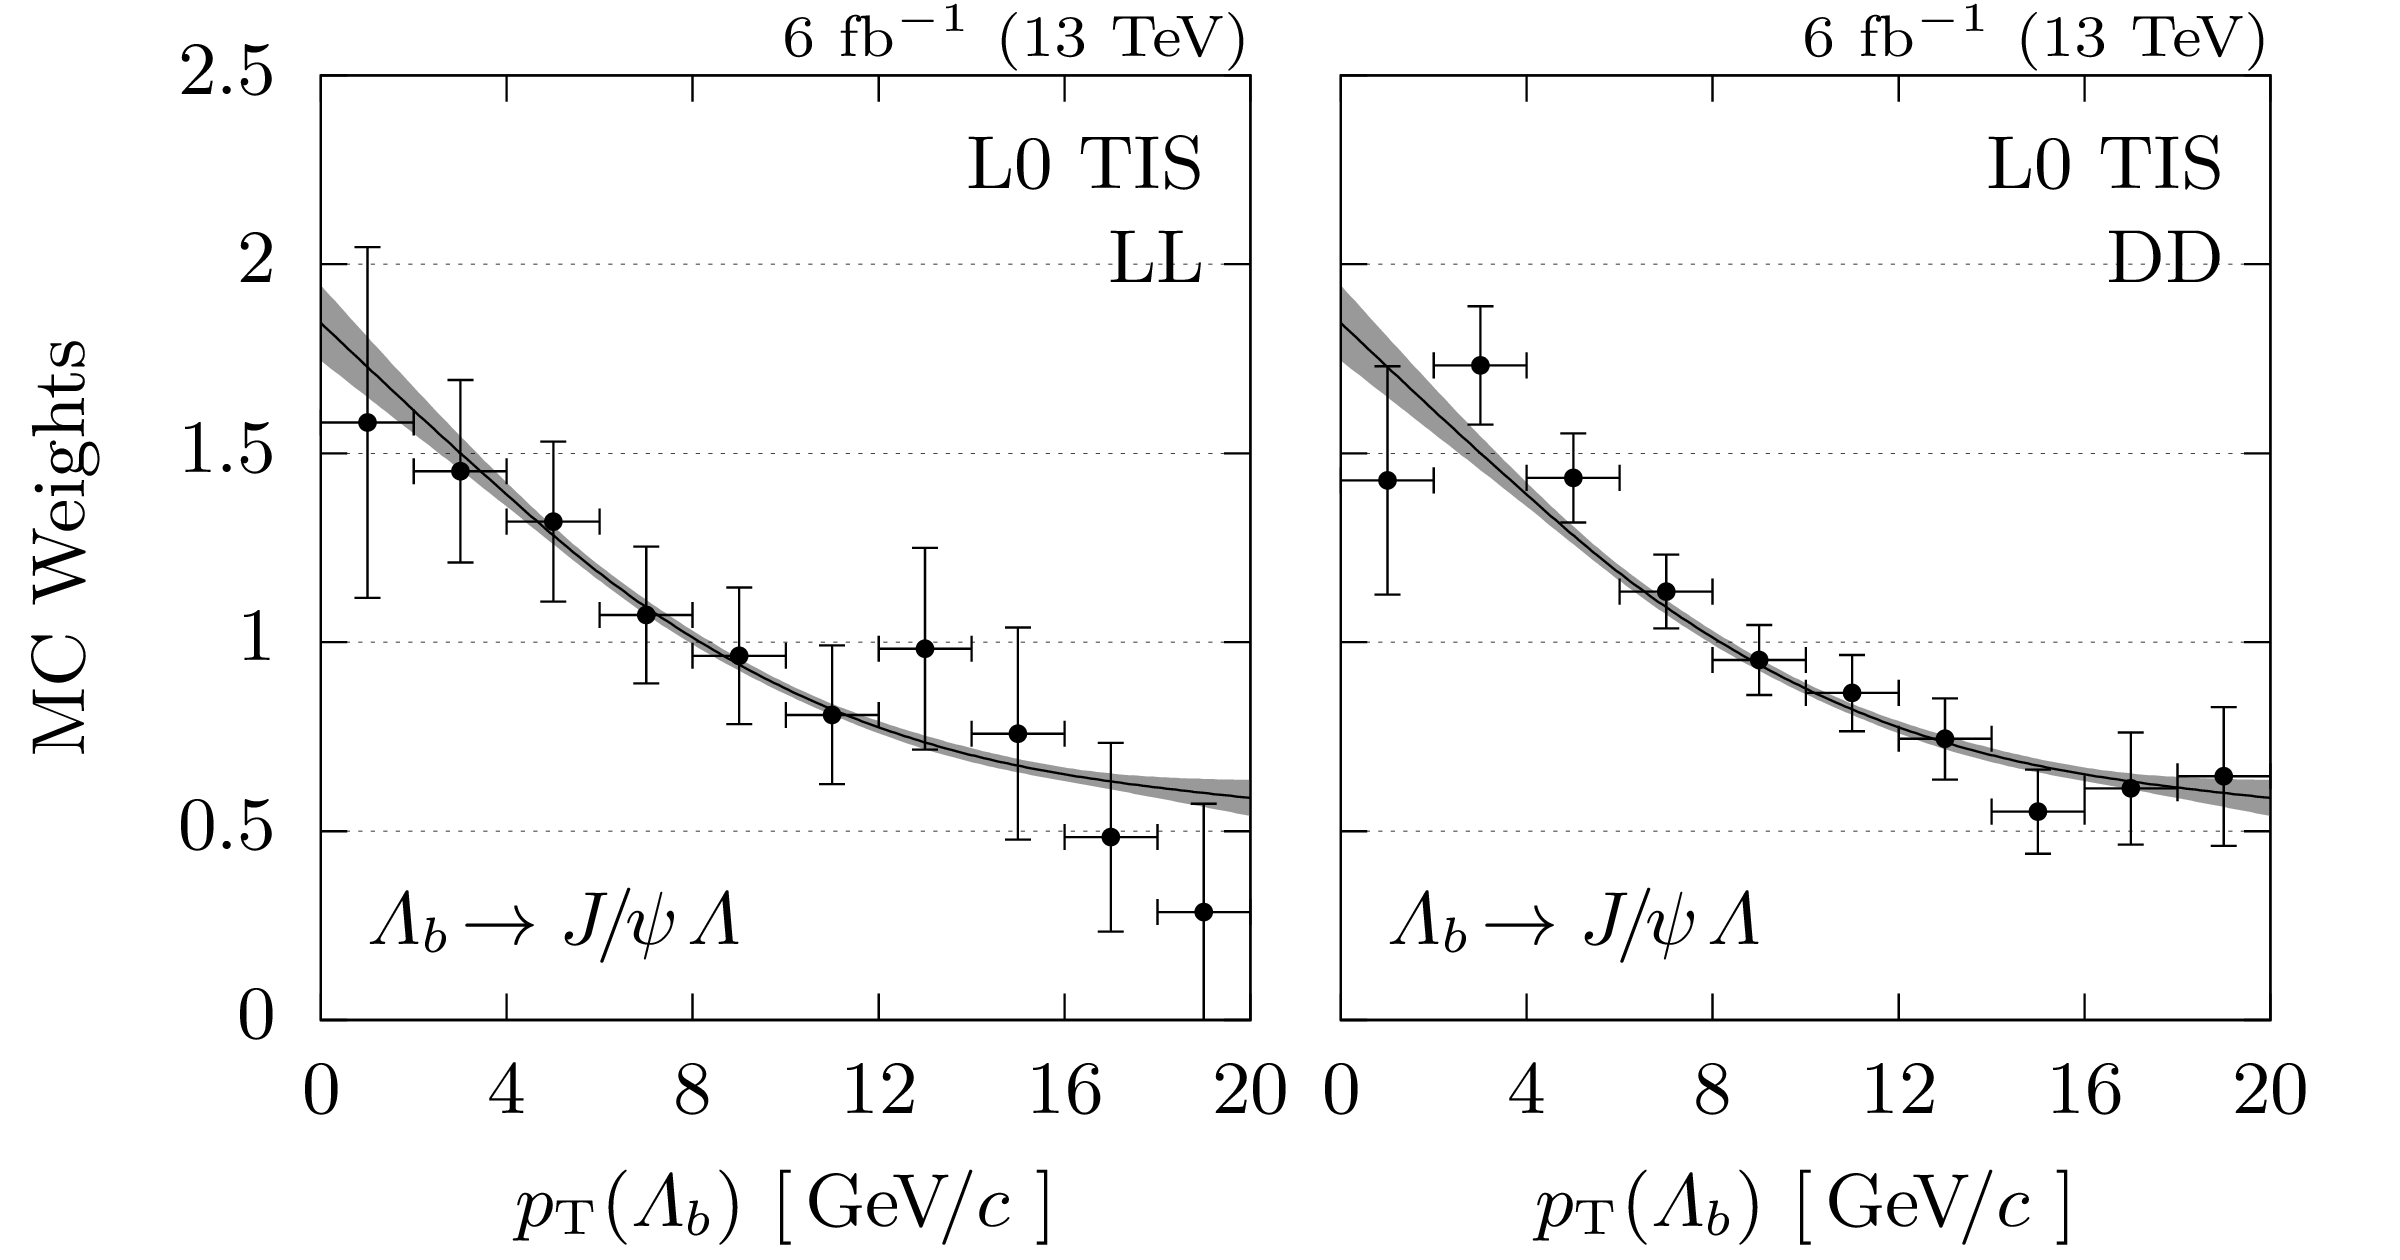
\includegraphics[scale=1.]{Lb2JpsiLz_weighting/weights_pT_avg.png}
    \end{subfigure}
    \par\bigskip 
    \begin{subfigure}{\textwidth}
        \centering
        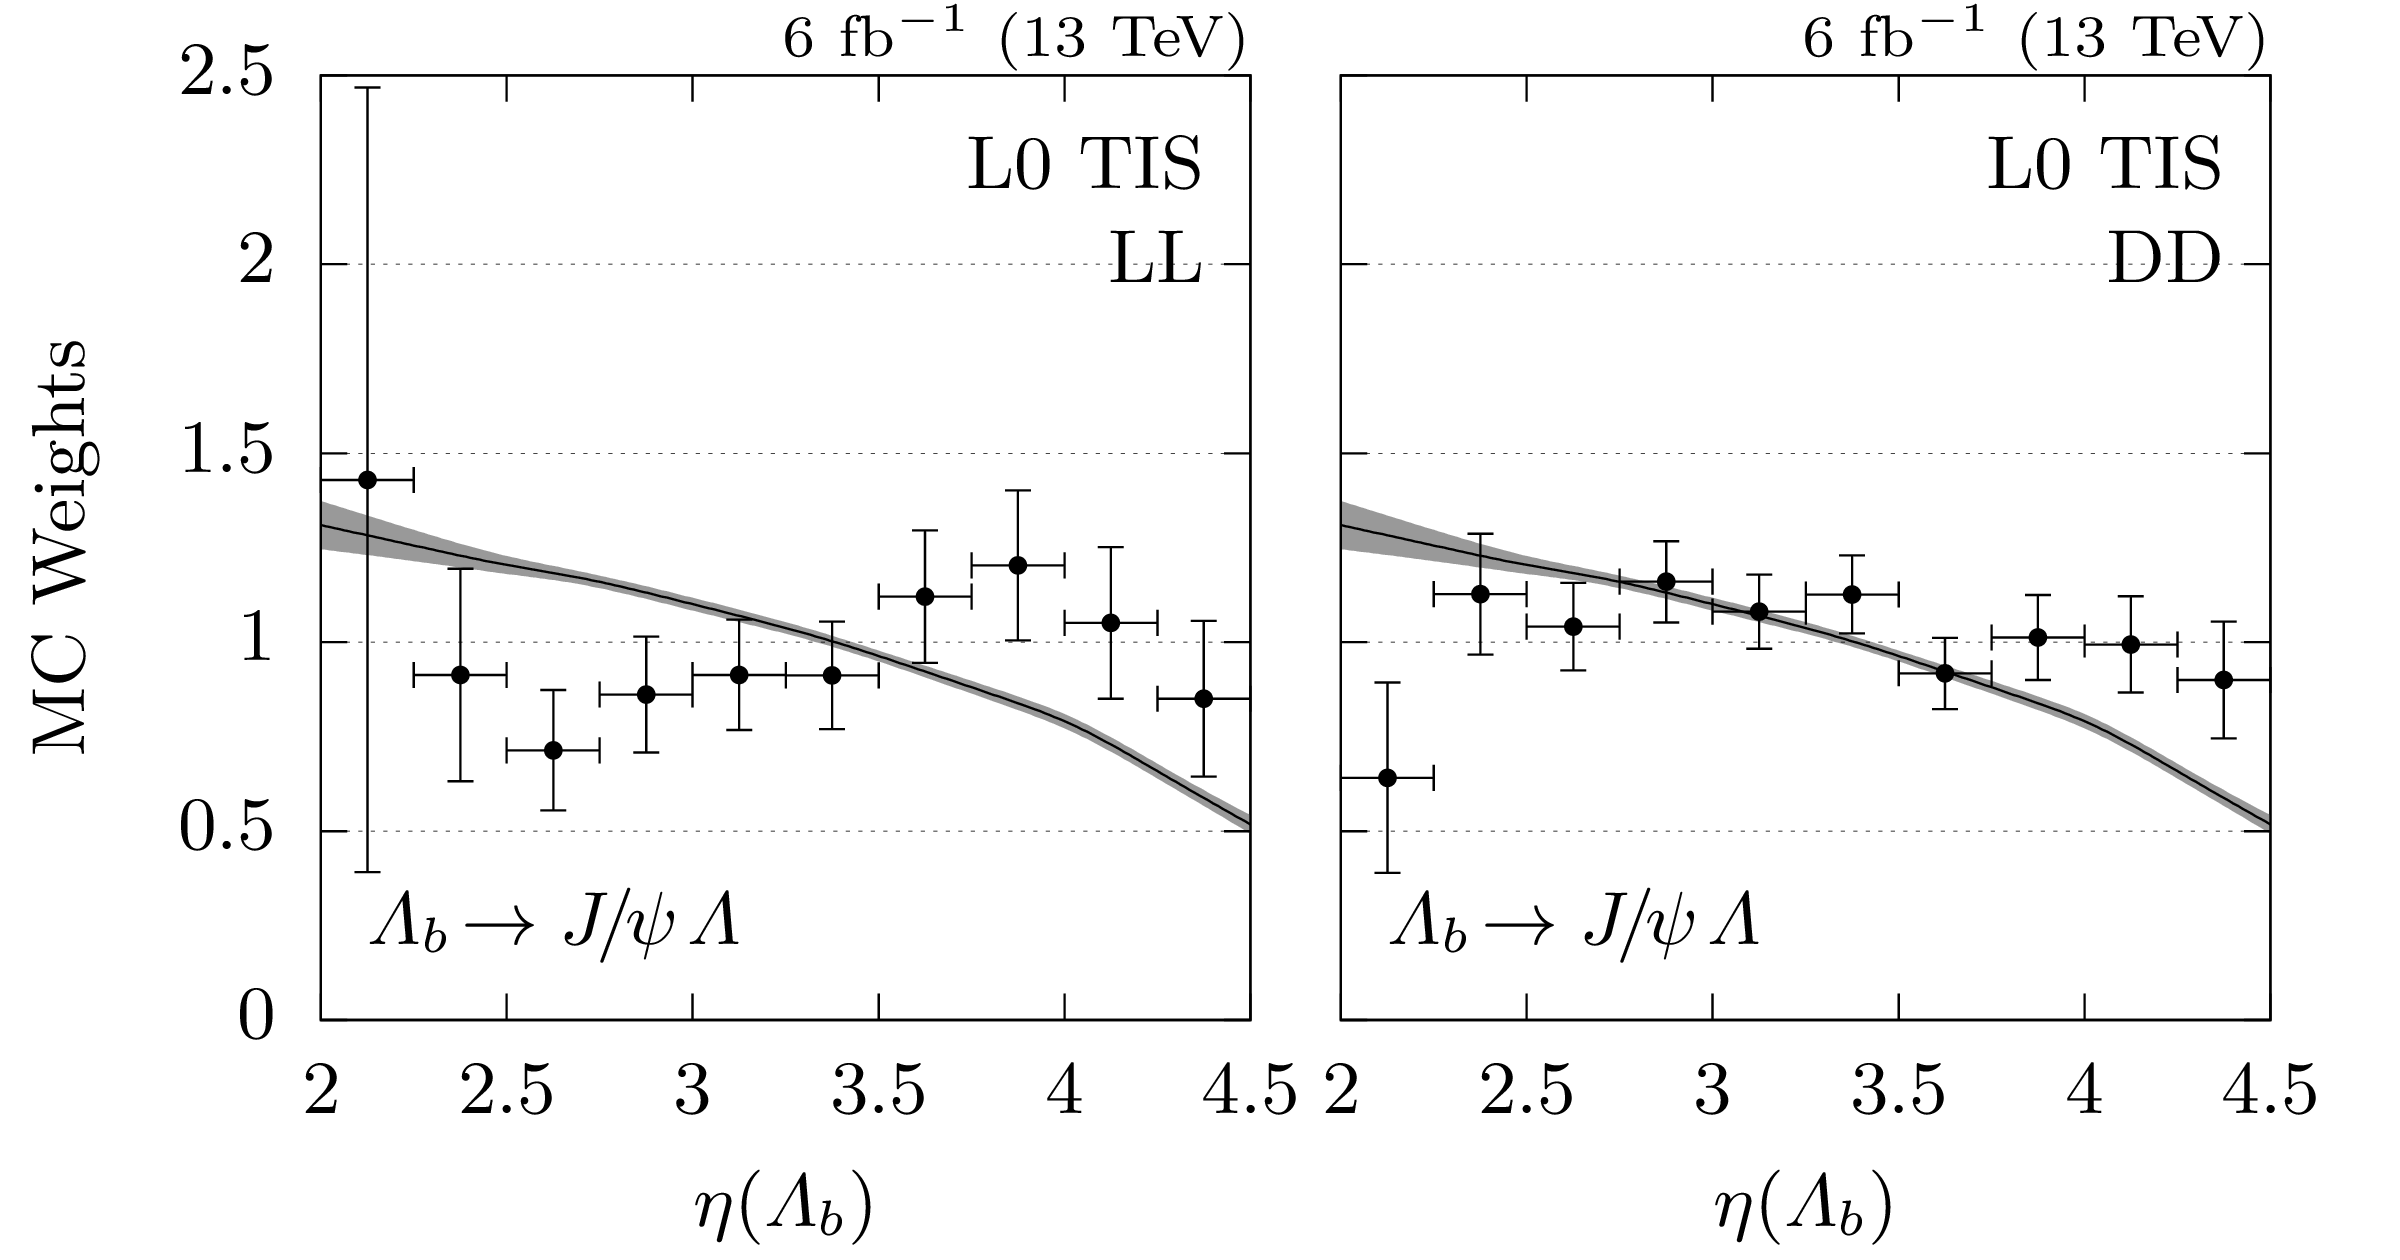
\includegraphics[scale=1.]{Lb2JpsiLz_weighting/weights_eta_avg.png}
    \end{subfigure}
    \caption{Averaged fit results of weights for \decay{\Lb}{\jpsi\Lz} (simultaneously for \gls{LL} and \gls{DD} tracks) and \decay{\Lb}{\Dz\proton\Km} events (taken from Ref.~\cite{hviemann}).}
    \label{fig:LbToJpsiLz_weights_avg}
\end{figure}

%The fit probability is approximately $99.7\,\%$ ($\chi^2 \approx 7$, \gls{dof}=$20$) and $83\,\%$ ($\chi^2 \approx 14$, \gls{dof}=$20$) for $w_1(\pt)$ and $w_2(\eta)$, respectively.

Since the weights $w_1(\pt)$ and $w_2(\eta)$ should neither depend on kinematic properties of \Lb daughters, nor on the decay channel itself, sensitivity is increased by combining our weights with weights extracted in a \decay{\Lb}{\Dz\proton\pim} analysis \cite{hviemann}.
(All final state particles are long tracks in this decay.)
We find a common set of weights by determining the weighted average of our simultaneously fitted $w(\pt, \eta)$ distribution and the corresponding one of the \decay{\Lb}{\Dz\proton\pim} analysis.
The fit results are shown in Fig.~\ref{fig:LbToJpsiLz_weights_avg} and exhibit a good agreement for $w_1(\pt)$, but large deviations for $w_2(\eta)$.
%(The latter predominantly arises from the larger statistics\footnote{The advantage of the higher statistics is compensated by the fact that the \decay{\Lb}{\jpsi\Lz} decay mode is much cleaner and easier to separate from background components.} of \decay{\Lb}{\Dz\proton\pim} at \lhcb.)
The combination reduces the statistical uncertainty and hints towards a difference between \gls{LL} and \gls{DD} that was already visible previously, but yet insignificant.
In comparison with the distributions of the non-normalized ratios of \gls{LL} and \gls{DD}, this difference is mostly promoted as an accumulation in the ratio of recorded and simulated data for \gls{LL} tracks and $\eta(\Lb) \gtrapprox 3.25$.

In Appx.~\ref{chap:apdx_weights} we summarize some investigations that exclude various possible explanations for the observed deviations in $w_2(\eta)$.
Eventually, the reason for this discrepancy stays unclear and motivates the second weighting scheme, outlined in the next section.

\subsection{Scheme 2}
\label{sec:LbToJpsiLz_w2}
In the considered sample of \decay{\Lb}{\jpsi\Lz} events, the weights $w_2(\eta)$ are compatible with one in good approximation, \cf{}~Tab.~\ref{tab:LbToJpsiLz_pvalues}.
Hence, a conservative approximation is to use $w(p_T, \eta) = 1 \times w'_2(p_T)$.
Since $p_T(\Lb)$ and $\eta(\Lb)$ are correlated, it is not sufficient to simply set $w_2(p_T) \equiv w_2'(p_T)$ in $w(p_T, \eta) = w_1(p_T) \times w_2(\eta)$.
Instead the ratio of recorded data and unweighted simulated events is taken as weights.
(Since there is only one variable, there is no need to perform this in an iterative approach.)

\begin{figure}[htbp]
    \centering
    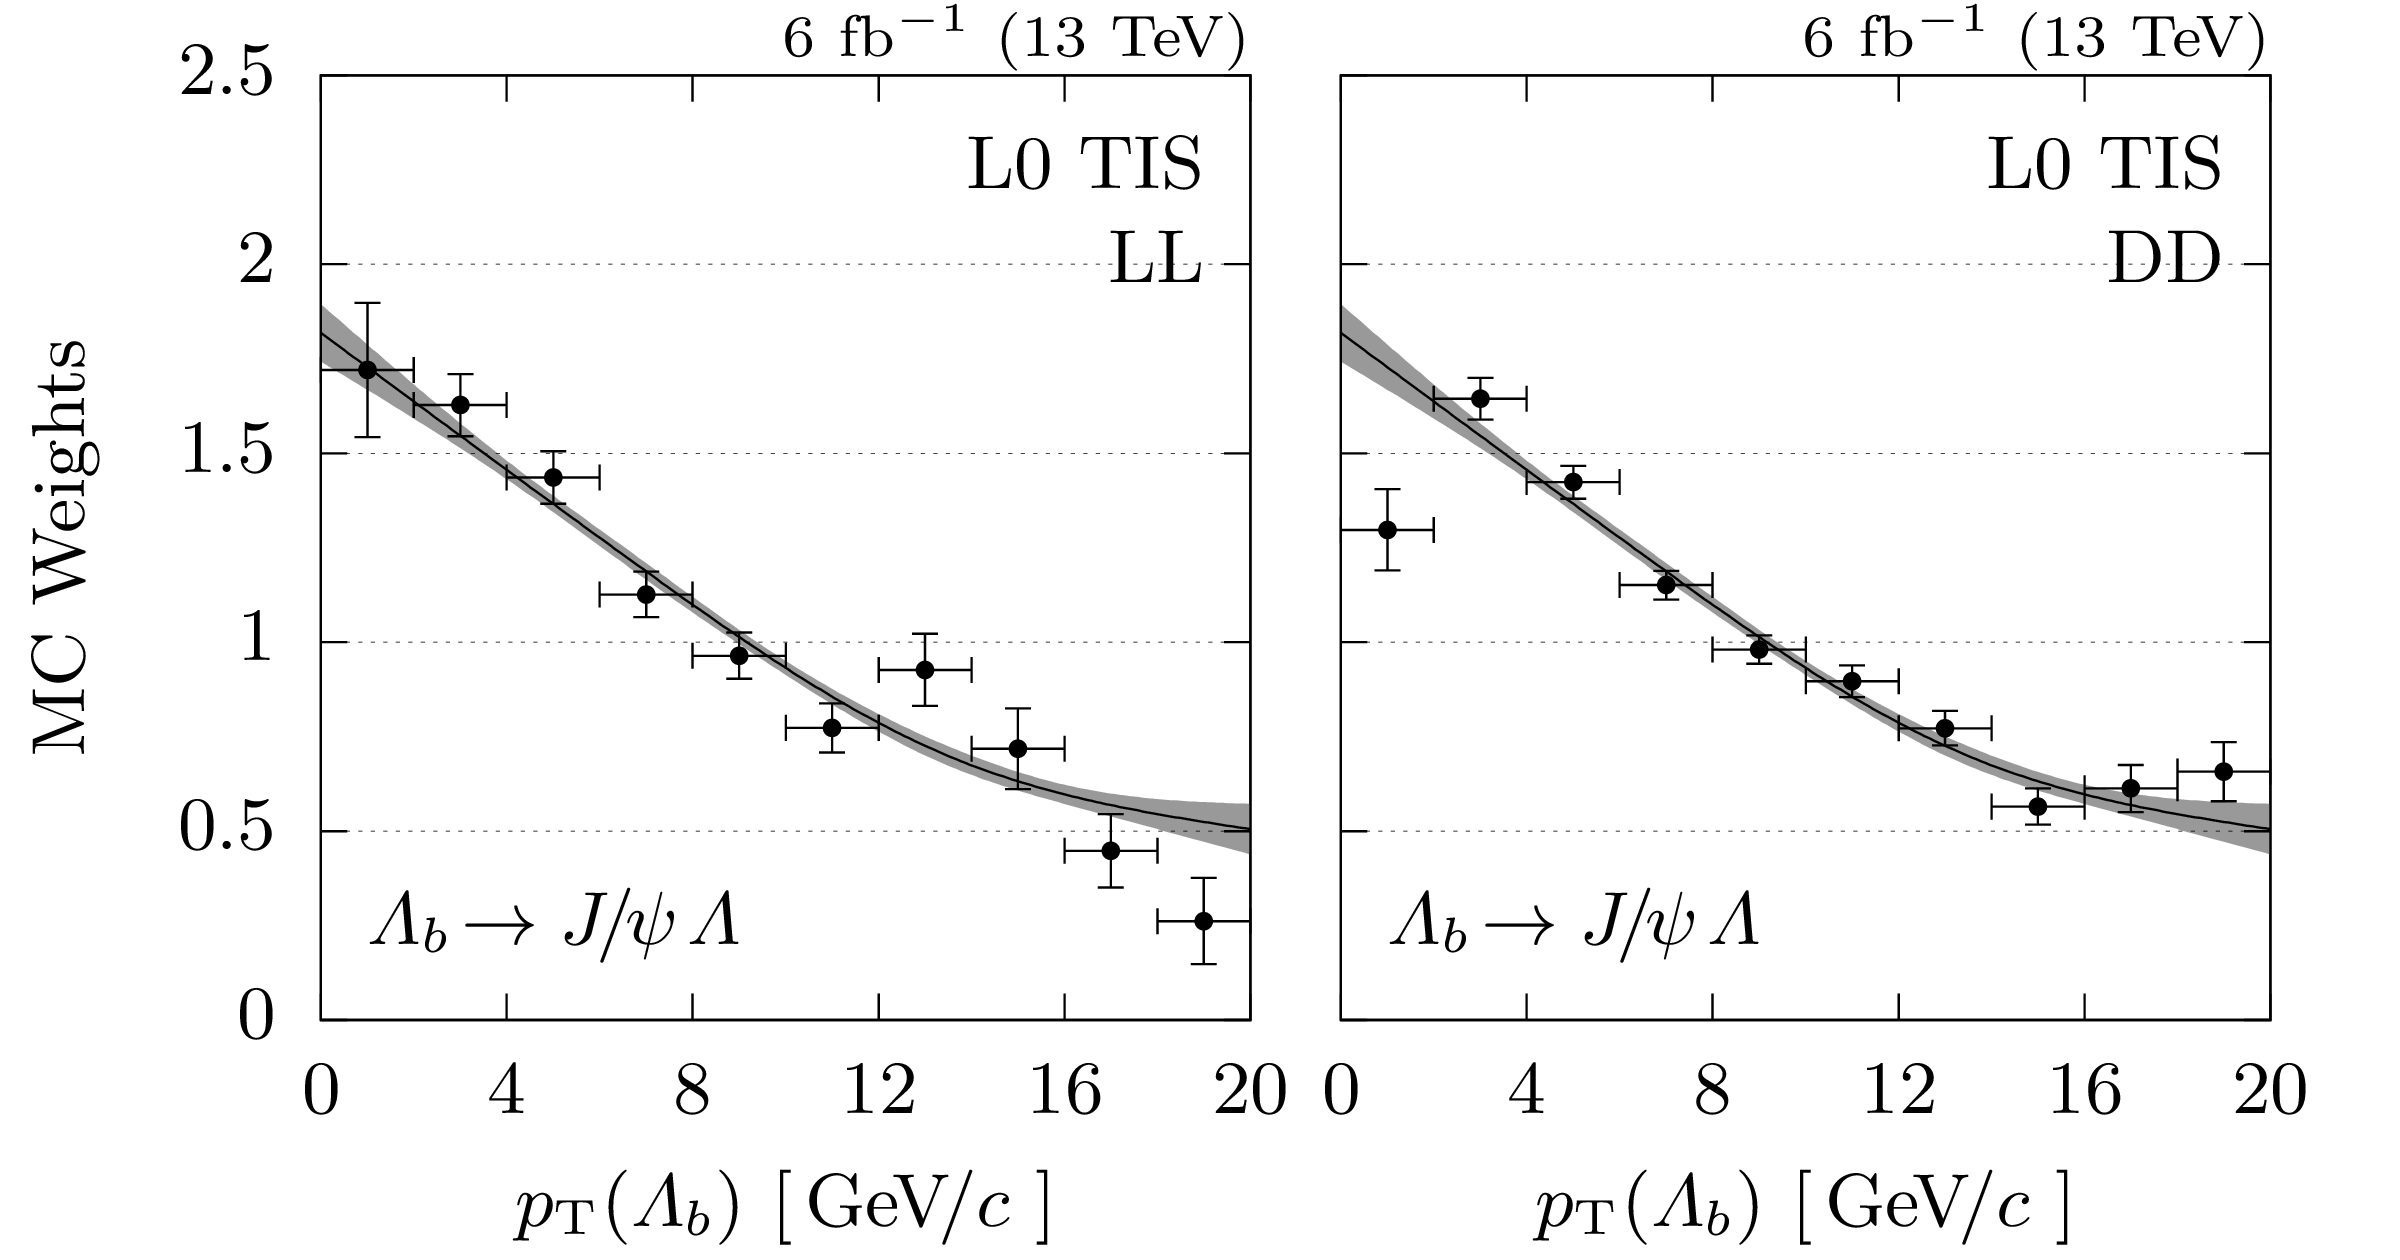
\includegraphics[scale=1.]{Lb2JpsiLz_weighting/weights_altfit.png}
    \caption{$\pt$-dependent weights obtained by weighting scheme 2, as well as spline fit, evaluated simultaneously for \gls{LL} and \gls{DD} tracks.}
    \label{fig:LbToJpsiLz_weights_altfit}
\end{figure}

The ratios are smoothed using a (natural) cubic spline with four \gls{dof} (\cf{}~Appx.~\ref{chap:csplines}).
Again, the spline is fitted simultaneously to \gls{LL} and \gls{DD} tracks.
Subsequently, the smoothed weights are used to weight the \gls{mc} simulated events.
The resulting distributions, as well as the corresponding spline fits for $\pt(\Lb)$ and both track types are shown in Fig.~\ref{fig:LbToJpsiLz_weights_altfit}.

In Fig.~\ref{fig:LbToJpsiLz_hratio_altfinal} we show the ratio of recorded data and weighted \gls{mc} simulated events for $\pt(\Lb)$ and $p(\Lb)$.
The combined $p$-values for both track types w.r.t.\ the hypothesis of a common underlying distribution for recorded and simulated events are approximately $8\,\%$ ($\chi^2 \approx 30$) and $0.1\,\%$ ($\chi^2 \approx 45$) for the $p(\Lb)$ and $\pt(\Lb)$ distributions, respectively.
These values do not include uncertainties of the spline fit and thus reflect only the $p$-value for a specific choice of weighting function.

\begin{figure}[htbp]
    \centering
    \begin{subfigure}{\textwidth}
        \centering
        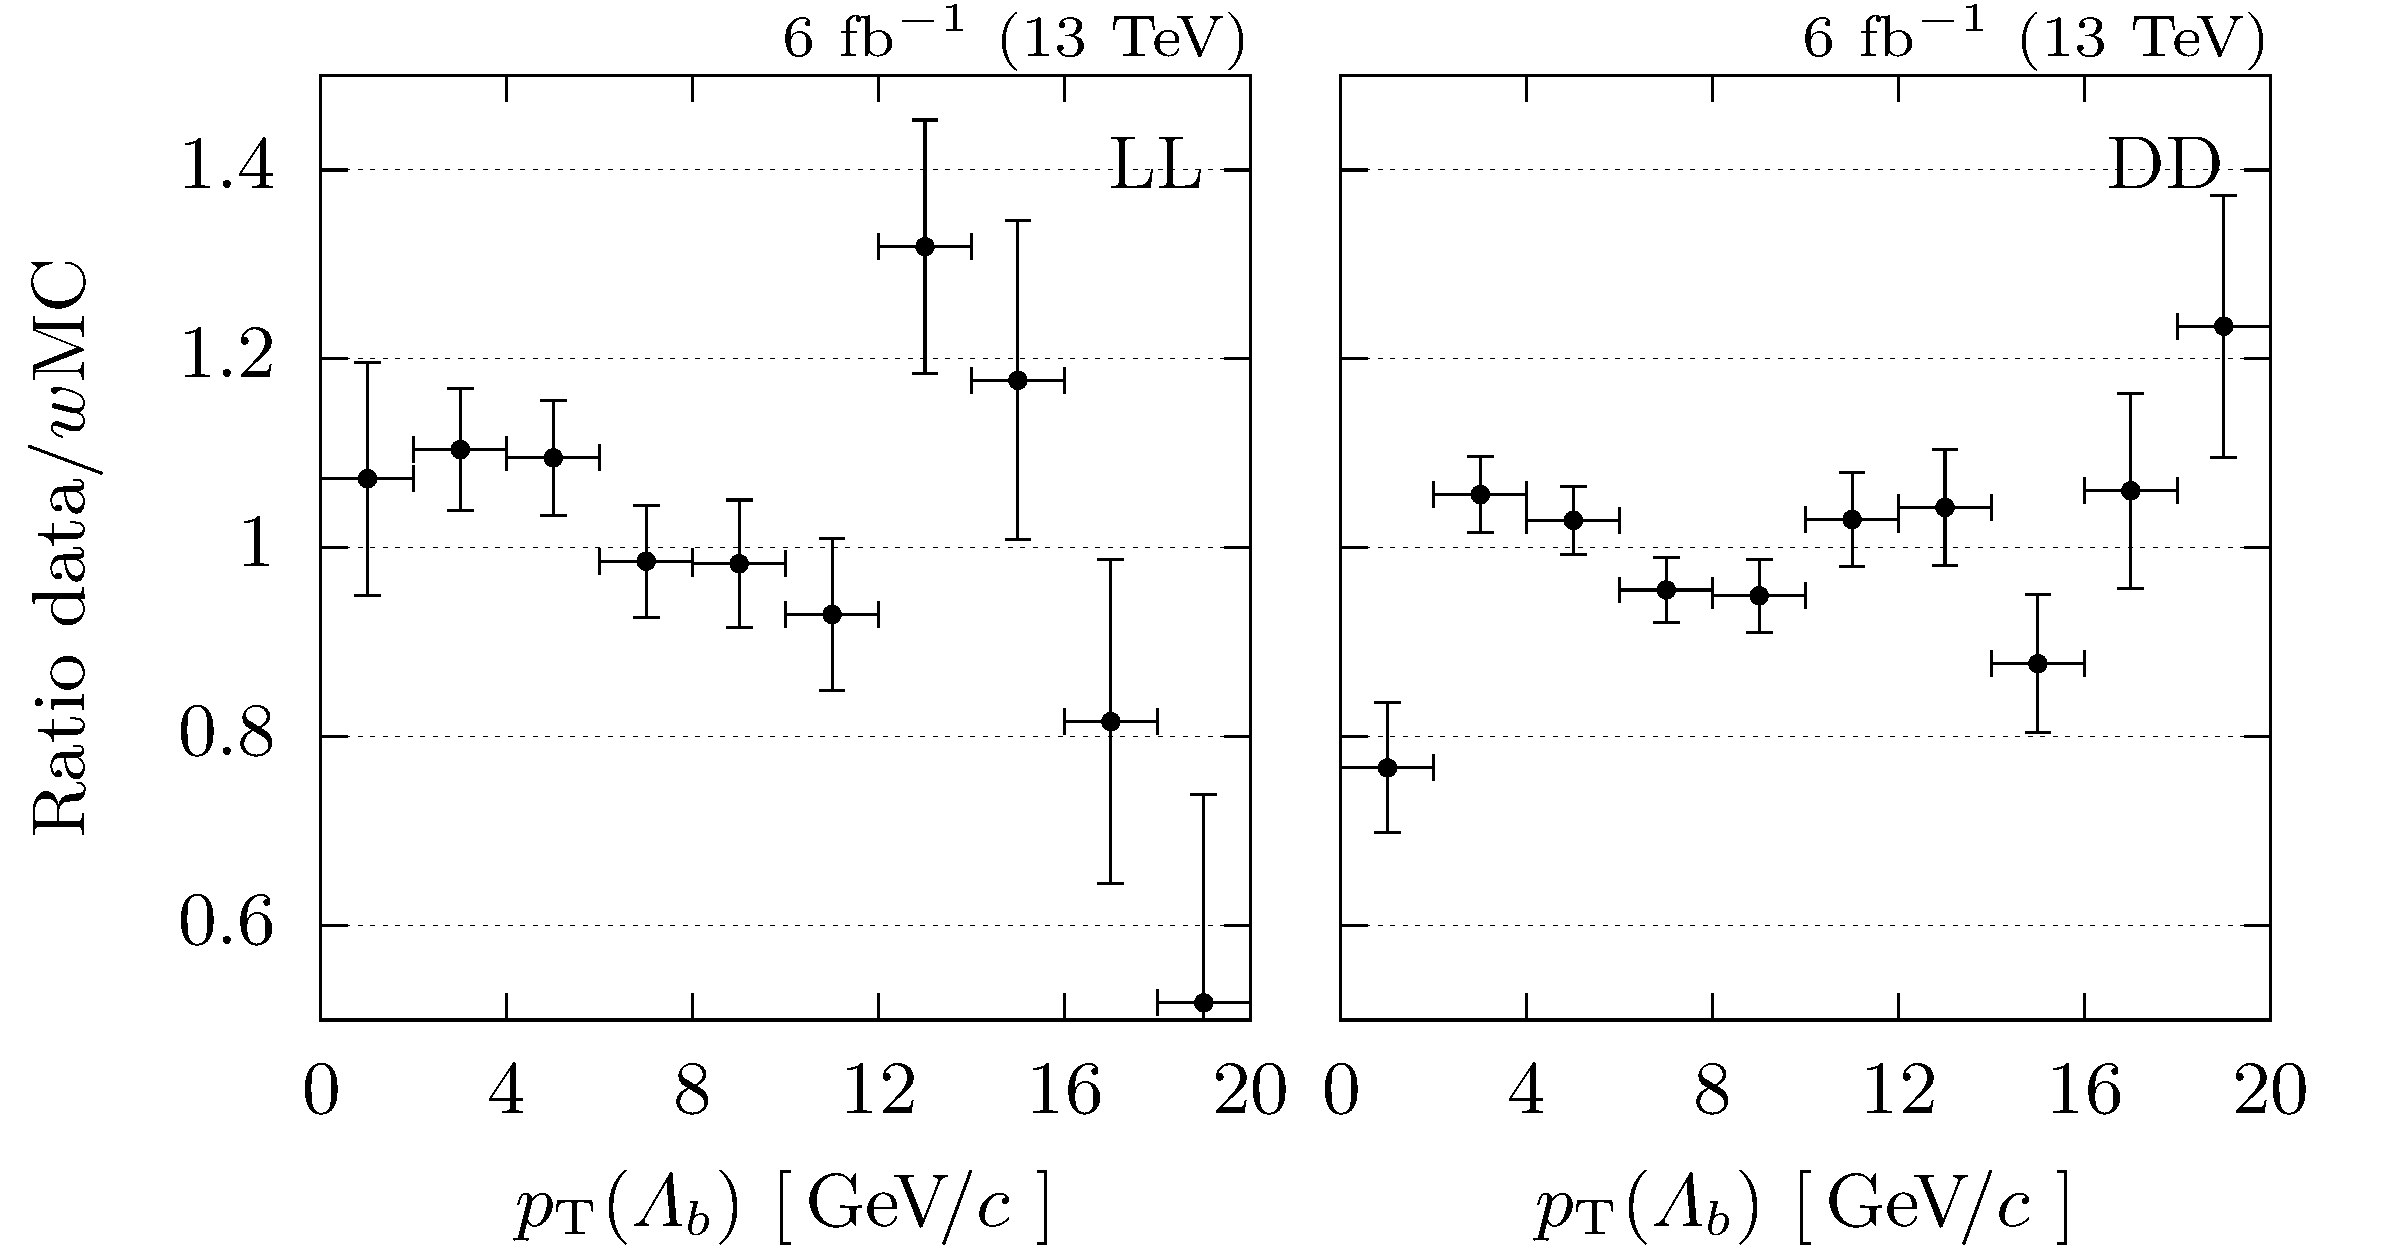
\includegraphics[scale=1.]{Lb2JpsiLz_weighting/hratio_pT_altfinal.png}
    \end{subfigure}
    \par\bigskip 
    \begin{subfigure}{\textwidth}
        \centering
        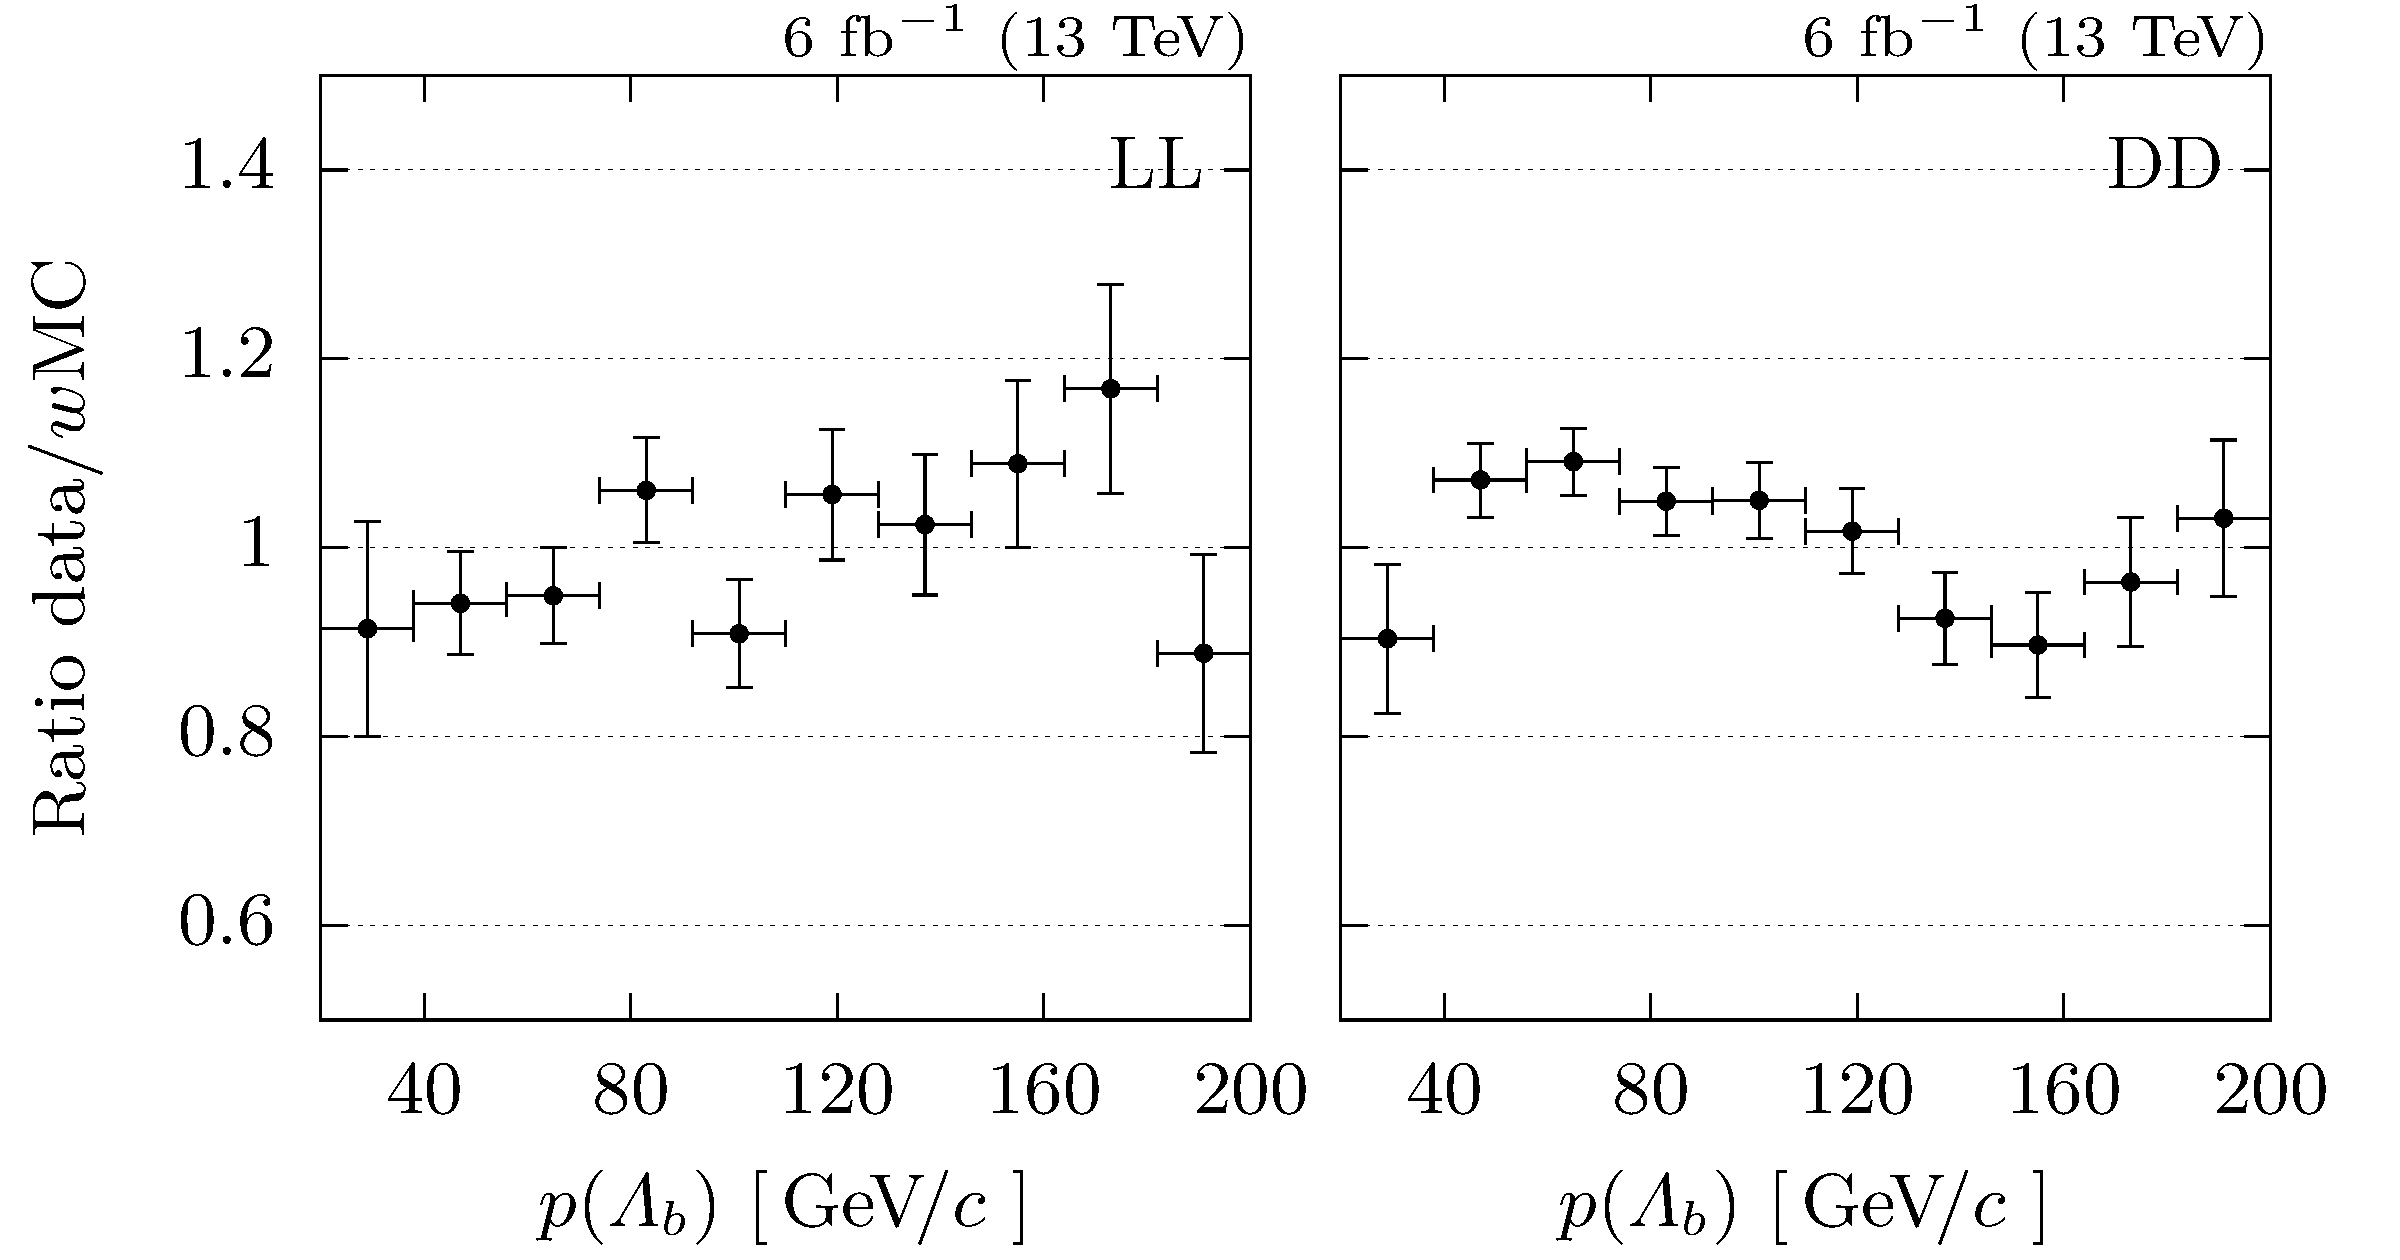
\includegraphics[scale=1.]{Lb2JpsiLz_weighting/hratio_p_altfinal.png}
    \end{subfigure}
    \caption{Ratio of recorded data and weighted \gls{mc} simulated events according to weighting scheme 2 for the transverse momentum of the \Lb baryon $\pt(\Lb)$ (top) and its three-momentum magnitude $p(\Lb)$ (bottom).}
    \label{fig:LbToJpsiLz_hratio_altfinal}
\end{figure}

\begin{frame}{How to find genuine decays? \textemdash Example \decay{\Lz}{\proton\pim}}
    \begin{columns}
        \begin{column}{.55\textwidth}
            \begin{itemize}
                \item Create \Lz candidates: $\{\Lz\} := \{\proton\} \otimes \{\pim\}$
                \item Use inv.\ mass $m(\Lz)\ftnt{} \overset{?}{=} m(\proton\pim)$ as proxy
                \item Separate components:
                \begin{enumerate}
                    \item Combinatorial background \\ \scalebox{.8}{(random track combinations)}
                    \item physical background \\ \scalebox{.8}{(\eg{}, \decay{\KS}{\textcolor{vertexDarkRed}{\pip}\pim})}
                    \item genuine \decay{\Lz}{\proton\pim} decays
                \end{enumerate}
            \end{itemize}
        \end{column}
        \begin{column}{.45\textwidth}
            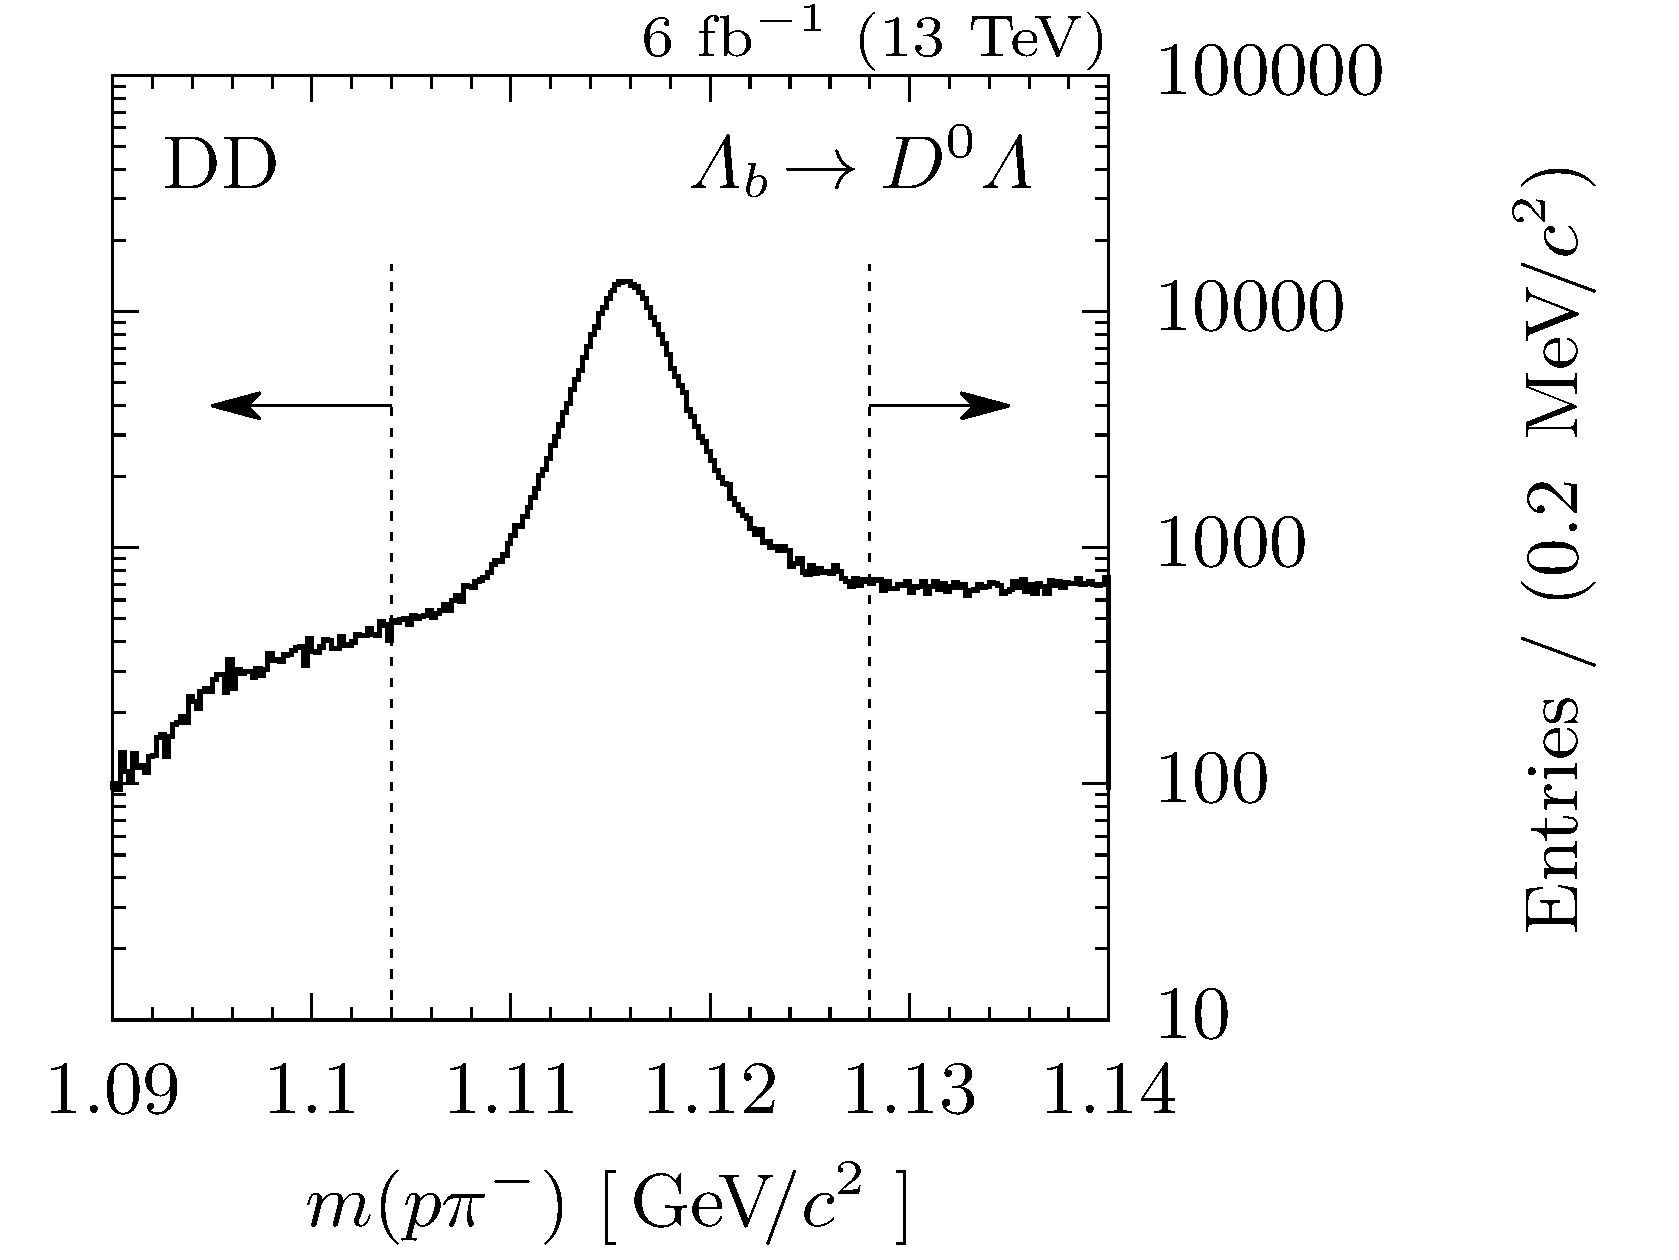
\includegraphics[width=\textwidth]{mvaLz/hLzM_DD}\\
            \hspace{5mm} \footnotesize (\ftnt PDG: $m(\Lz) \approx 1.117\gevcc$)
        \end{column}
    \end{columns}

    \vspace{5mm}

    \scalebox{0.8}{\vbox{%
    Technical detail: only (weak) Cabibbo suppressed decays possible for \Lz
    \vspace{-2mm}
    \begin{itemize}
        \item \textit{long} lifetime
        \item some \Lz decay outside (inside) of first detector element: refer to as \textbf{DD} (\textbf{LL})
        \item different detector response, separate analysis necessary
    \end{itemize}}}
\end{frame}

\begin{frame}[plain,noframenumbering]
    \centering
    \scalebox{2.}{Do the same for \decay{\Lb/\Xibz}{\Dz\Lz}?}

    \ie{}, $\{ \Lb/\Xibz \} := \underbrace{\{ \Km \} \otimes \{ \pip \}}_{\{ \Dz \}} \otimes \underbrace{\{ \proton \} \otimes \{ \pim \}}_{\{ \Lz \}}$
\end{frame}

\begin{frame}{Searching for \decay{\Lb/\Xibz}{\Dz\Lz}}
    \begin{columns}
        \begin{column}{.55\textwidth}
            \textbf{No signal visible!}
            \begin{itemize}
                \item Background (at this stage) mainly combinatorial
                \item Need to increase
                \begin{itemize}
                    \item purity of $\{ \Dz \}$
                    \item purity of $\{ \Lz \}$
                    \item filter $\{ \Dz \} \otimes \{ \Lz \}$ for $\decay{\Lb/\Xibz}{\Dz\Lz}$ decays by constraining physical properties
                \end{itemize}
                \item (Carefully analyse physical backgrounds\ftntdagger)
            \end{itemize}
        \end{column}
        \begin{column}{.45\textwidth}
            \only<1>{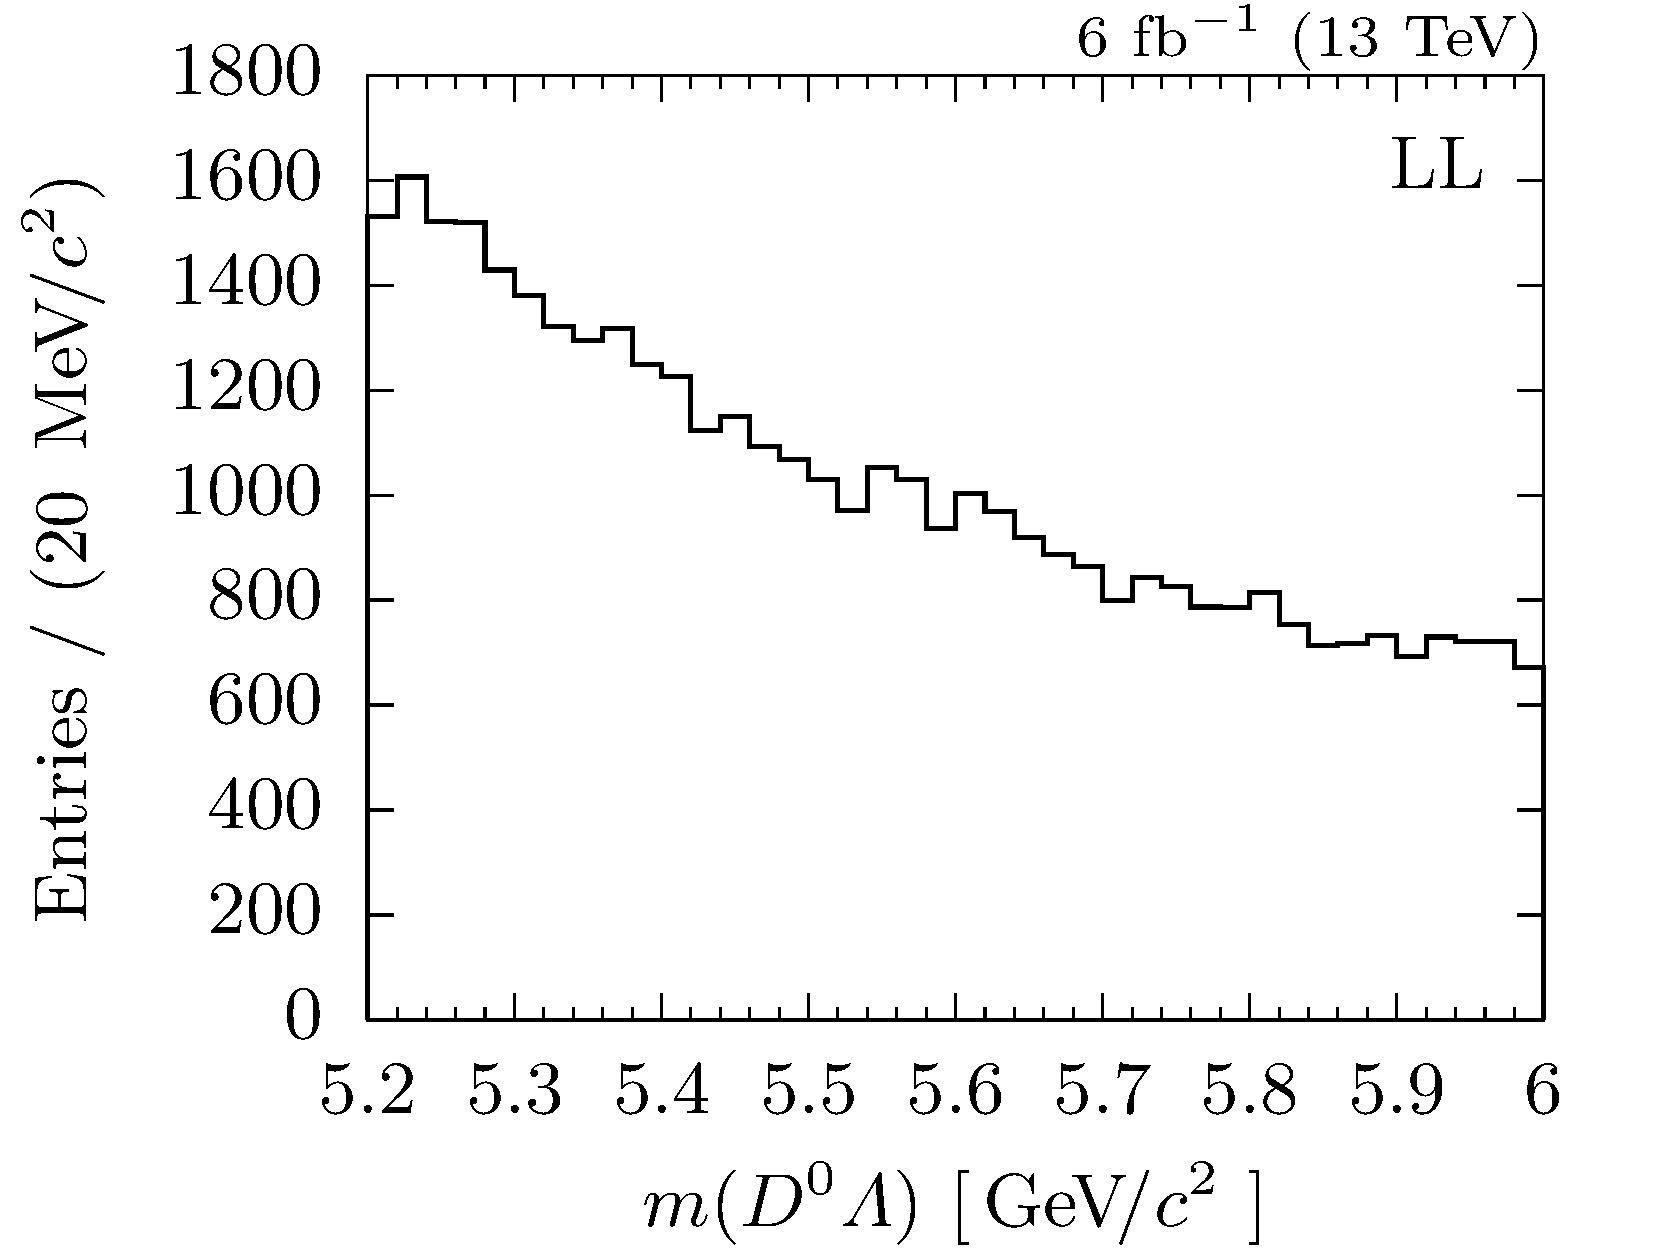
\includegraphics[width=\textwidth]{mvaLbDz/hDzLzM_LL}}%
            \only<2>{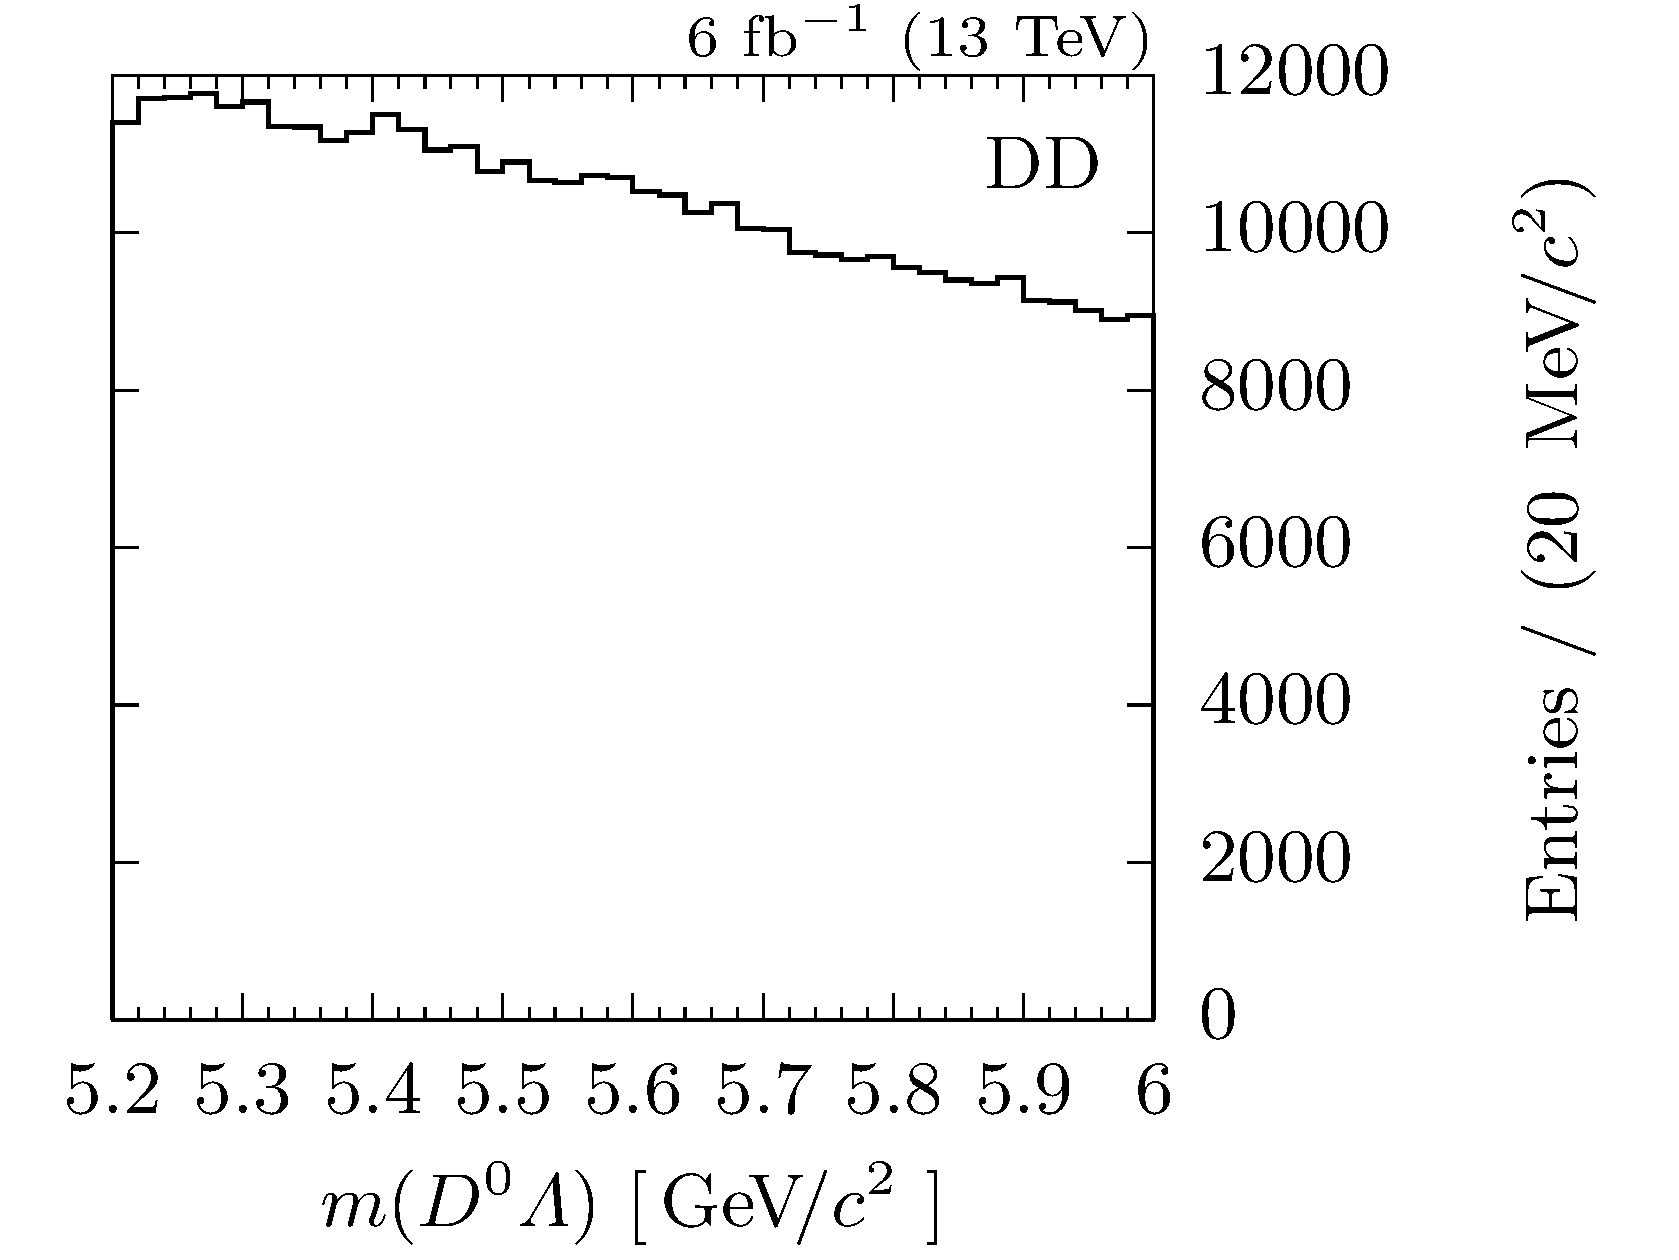
\includegraphics[width=\textwidth]{mvaLbDz/hDzLzM_DD}}%
            \\
            \hspace{5mm} \footnotesize (PDG: $m(\Lb) \approx 5.620\gevcc$,\\
            \hspace{5mm} \footnotesize \phantom{(}PDG: $m(\Xibz) \approx 5.792\gevcc$)
        \end{column}
    \end{columns}
\end{frame}

\begin{frame}{Searching for \decay{\Lb/\Xibz}{\Dz\Lz}}
    \begin{columns}
        \begin{column}{.6\textwidth}
            \textbf{Use ML to rescue!} Classification problem
            \begin{itemize}
                \item Separate \textit{\textbf{signal}} (genuine \decay{\Lb/\Xibz}{\Dz\Lz})
                \item \ldots from (combinatorial) \textit{\textbf{background}}
                \item Labels?
                \begin{itemize}
                    \item use MC simulated decays for class \textit{signal}\ftntdagger{}
                    \item use recorded data from sidebands for class \textit{background}
                \end{itemize}
            \end{itemize}
        \end{column}
        \begin{column}{.4\textwidth}
            \centering
            
\includegraphics[width=.5\textwidth]{needle_haystack}\\
            {\tiny (Image: R.~Diepenheim on \texttt{thenounproject.com})}
        \end{column}
    \end{columns}

    \vspace{5mm}

    \footnotesize \ftntdagger{} calibration needed (not discussed here)
\end{frame}

\begin{frame}{MVA methodoloy}
    \begin{tikzpicture}[>=triangle 45,
                        node/.style={rectangle,align=center,rounded corners}]
        \node[draw,node] (data) {$X, y, w$};
        \node[draw,node,right=1cm of data] (presel) {Loose / \\ (pre-)selection\ftntdagger};
        \node[draw,node,right=2cm of presel] (pProbNNp) {\texttt{ProbNNp}\ftnt{}};
        \node[draw,node,above=.5cm of pProbNNp] (clfLbDz) {\Lb-\Dz classifier};
        \node[draw,node,above=.5cm of clfLbDz] (clfLz) {\Lz classifier};
        \node[draw,node,below=.5cm of pProbNNp] (kProbNNk) {\texttt{ProbNNk}\ftnt{}};
        \node[draw,node,below=.5cm of kProbNNk] (dtf) {DTF prob.};
        \node[draw,node,right=2cm of pProbNNp] (fclf) {Rectangular\\ cut classifier};

        \draw[->] (data) -- (presel);
        \draw[->] (presel) -- (pProbNNp);
        \draw[->] (presel.north east) + (0,-1mm) -- (clfLz.west);
        \draw[->] (presel.north east) + (0,-3mm) -- (clfLbDz.west);
        \draw[->] (presel.south east) + (0, 3mm) -- (kProbNNk.west);
        \draw[->] (presel.south east) + (0, 1mm) -- (dtf.west);
        \draw[->] (pProbNNp) -- (fclf);
        \draw[->] (clfLz.east) -- ($(fclf.north west) + (0,-1mm)$);
        \draw[->] (clfLbDz.east) -- ($(fclf.north west) + (0,-3mm)$);
        \draw[->] (kProbNNk.east) -- ($(fclf.south west) + (0,3mm)$);
        \draw[->] (dtf.east) -- ($(fclf.south west) + (0,1mm)$);
    \end{tikzpicture}

    \textbf{Training:} classify $m$ data $X \in \mathbb{R}^{m \times n}$ with $n$ features using labels $y \in \{ \text{sig.}, \text{bkg.} \}^m$ and calibration factors\ftntdagger{} $w \in \mathbb{R}^m$ with $\mathcal{O}(m) = 10k$, $n = 18$

    \vspace{5mm}
    \footnotesize \ftnt{} pre-trained shallow NN
\end{frame}

\begin{frame}{Example: \Lz classifier}
    \begin{columns}
        \begin{column}{.55\textwidth}
            \begin{itemize}
                \item 5 features of $\{ \Lz \}$: 
                \begin{enumerate}
                    \item transverse momentum
                    \item angle between momentum and connecting line between \proton\proton-IA point (PV) and \Lz decay vertex
                    \item $\chi^2$ improvement of PV with \Lz track
                    \item fit prob.\ of decay vertex
                    \item significance of flight distance
                \end{enumerate}
                \item Separate classifiers for LL and DD
                \item Optimize hyper-parameters of 5 classifiers using grid search w.r.t.\ ROC-AUC\ftnt{} value
            \end{itemize}
        \end{column}
        \begin{column}{.45\textwidth}
            \centering
            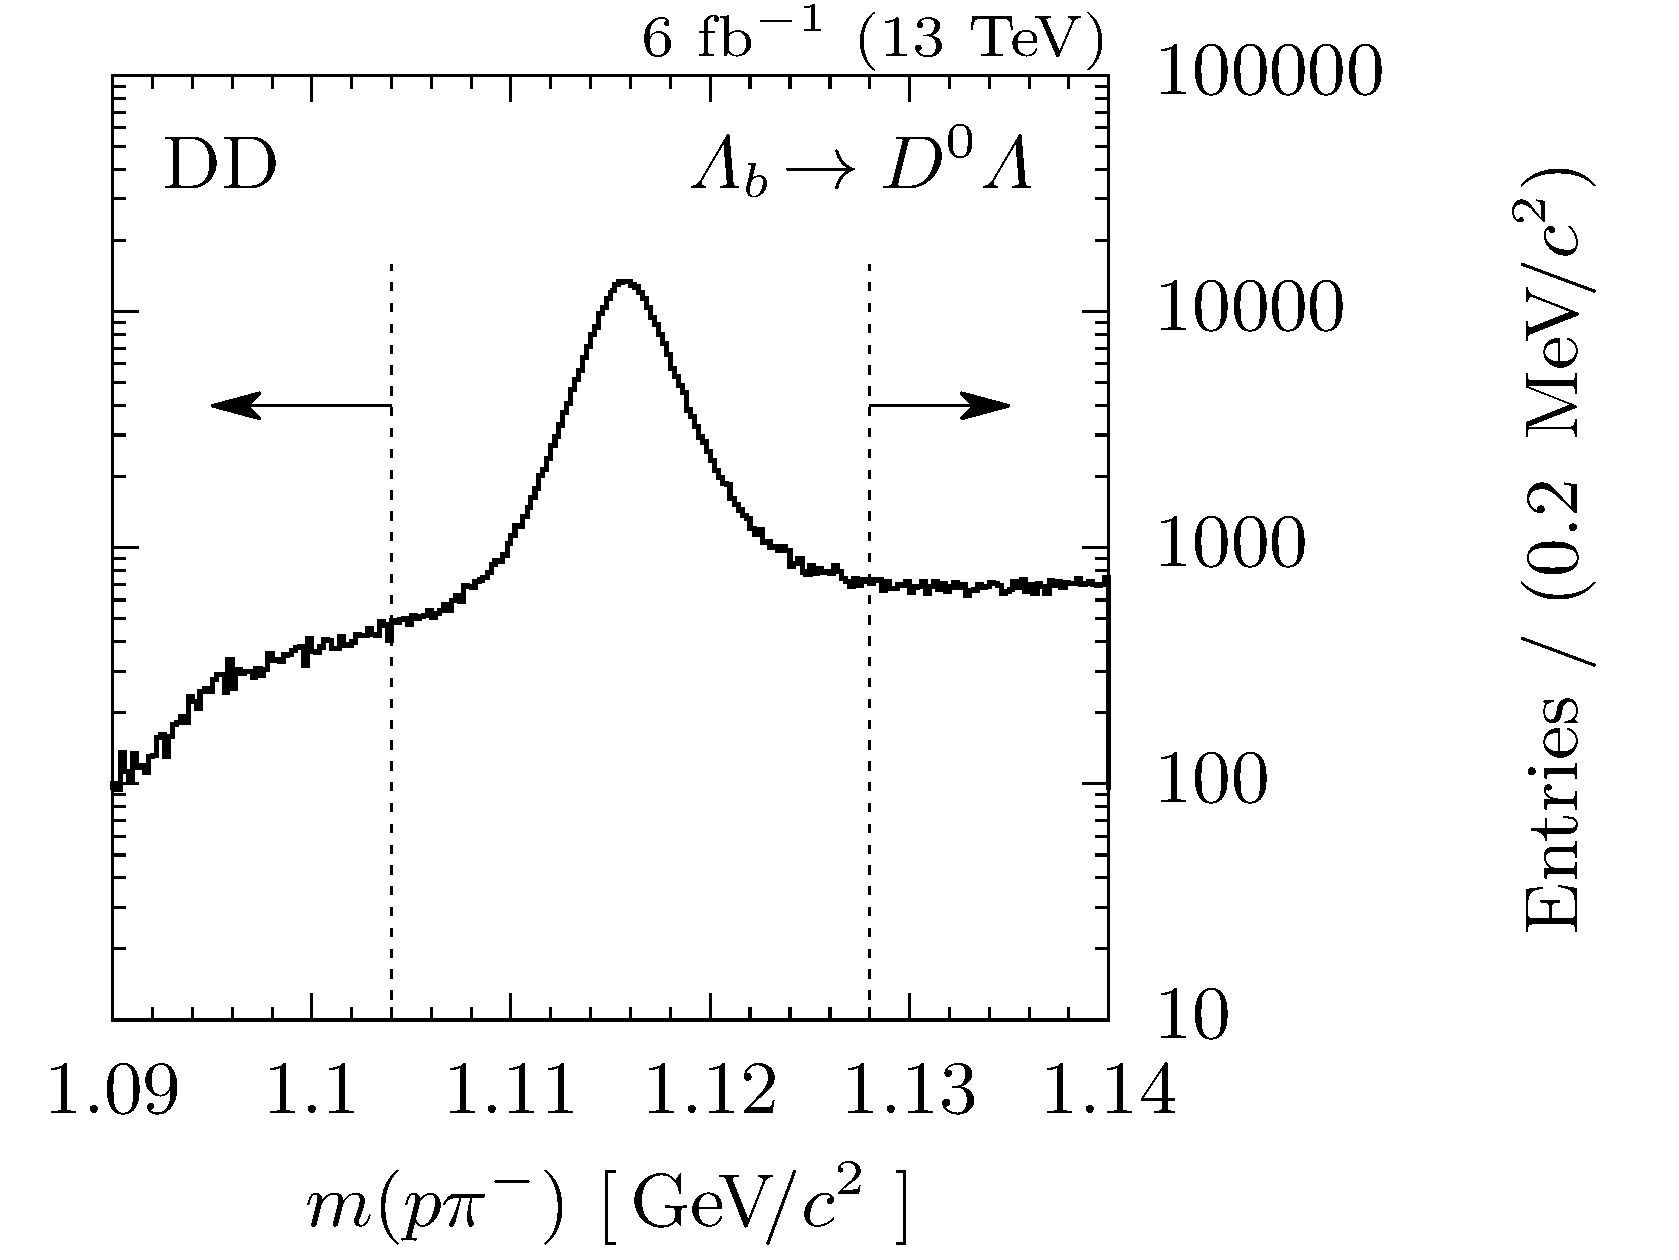
\includegraphics[scale=1.]{mvaLz/hLzM_DD}
        \end{column}
    \end{columns}

    \vspace{5mm}
    \footnotesize \ftnt{} Prob.\ that clf.\ will rank randomly chosen \textit{sig.} instance higher than randomly chosen \textit{bkg.} one
\end{frame}

\begin{frame}{Example: \Lz classifier}
    \begin{columns}
        \begin{column}{.45\textwidth}
            \scalebox{1.2}{\Lz classifier}
            \begin{itemize}
                \item \textcolor{vertexDarkRed}{5 features of $\{ \Lz \}$}
                \item Separate classifiers for LL and \textbf{DD}
                \item Optimize hyper-parameters of 5 classifiers using grid search w.r.t.\ ROC-AUC\ftnt{} value
            \end{itemize}
        \end{column}
        \begin{column}{.5\textwidth}
            \centering
            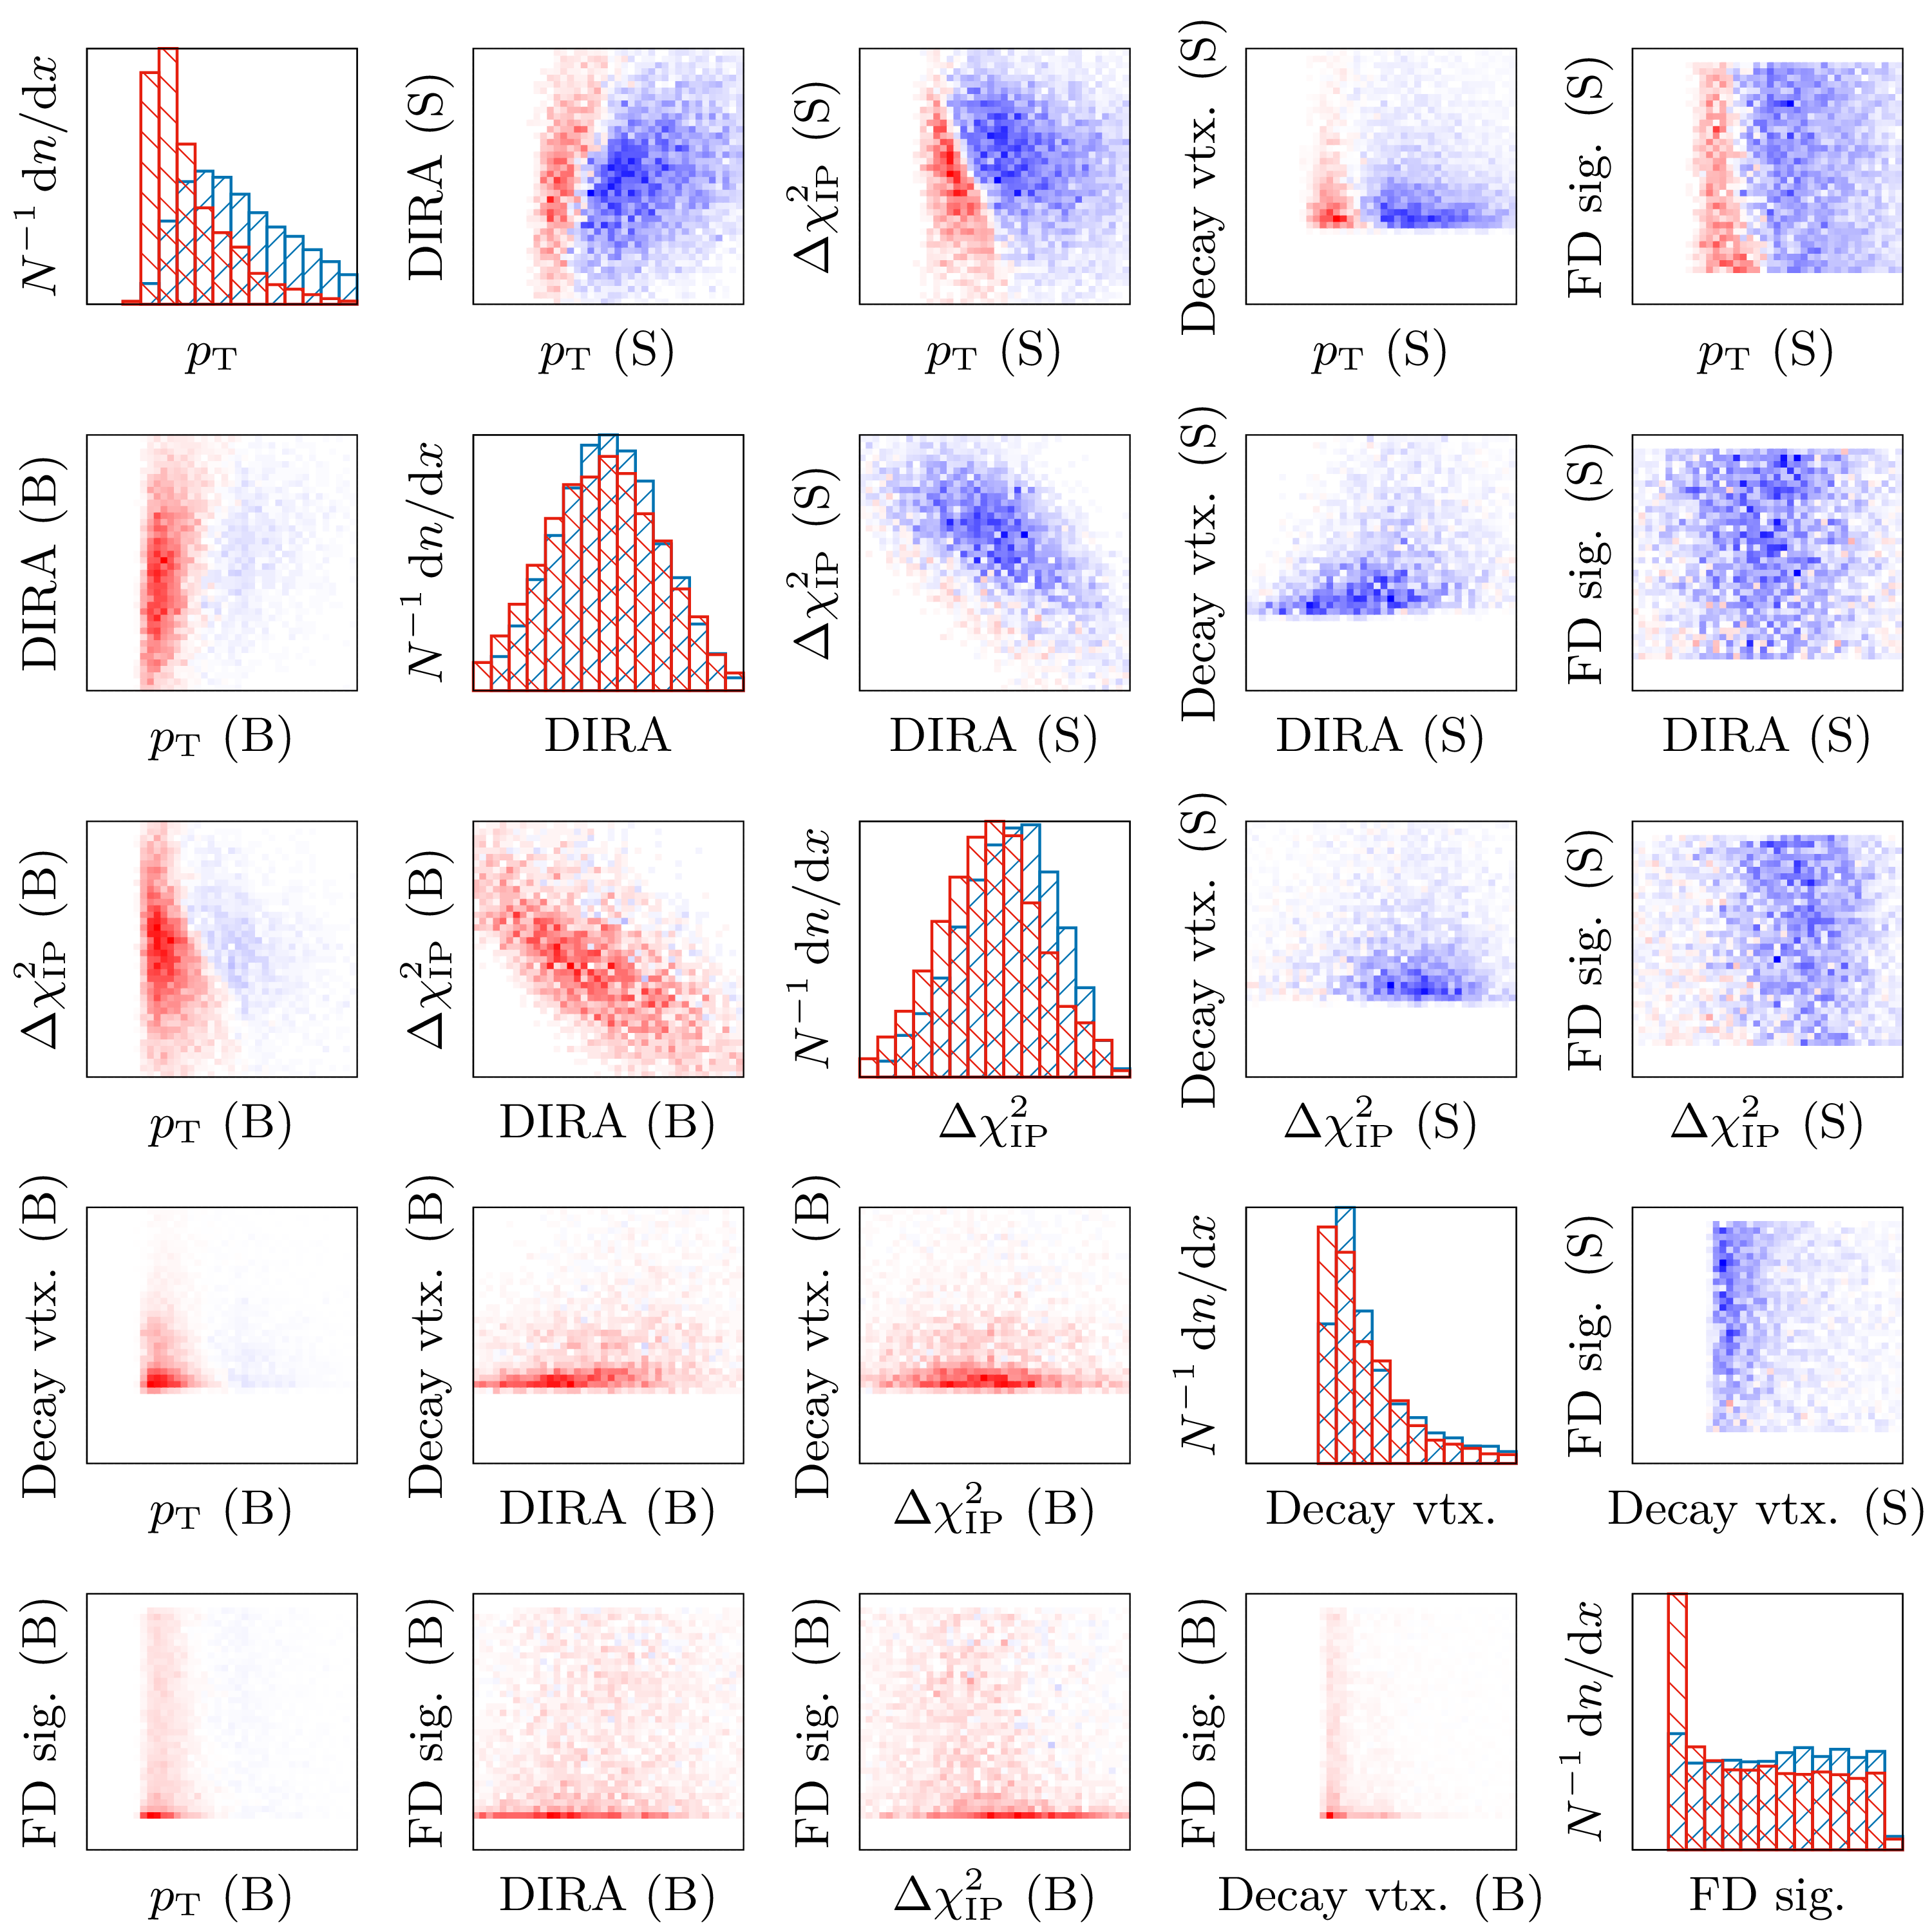
\includegraphics[height=.9\textheight]{mvaLz/mvaLz_corr_DD}\\
            (track type \textbf{DD})
        \end{column}
    \end{columns}
\end{frame}

\begin{frame}{Example: \Lz classifier}
    \begin{columns}
        \begin{column}{.45\textwidth}
            \scalebox{1.2}{\Lz classifier}
            \begin{itemize}
                \item 5 features of $\{ \Lz \}$
                \item Separate classifiers for LL and \textbf{DD}
                \item Optimize hyper-parameters of \textcolor{vertexDarkRed}{5 classifiers} using grid search w.r.t.\ ROC-AUC\ftnt{} value
            \end{itemize}
        \end{column}
        \begin{column}{.5\textwidth}
            \centering
            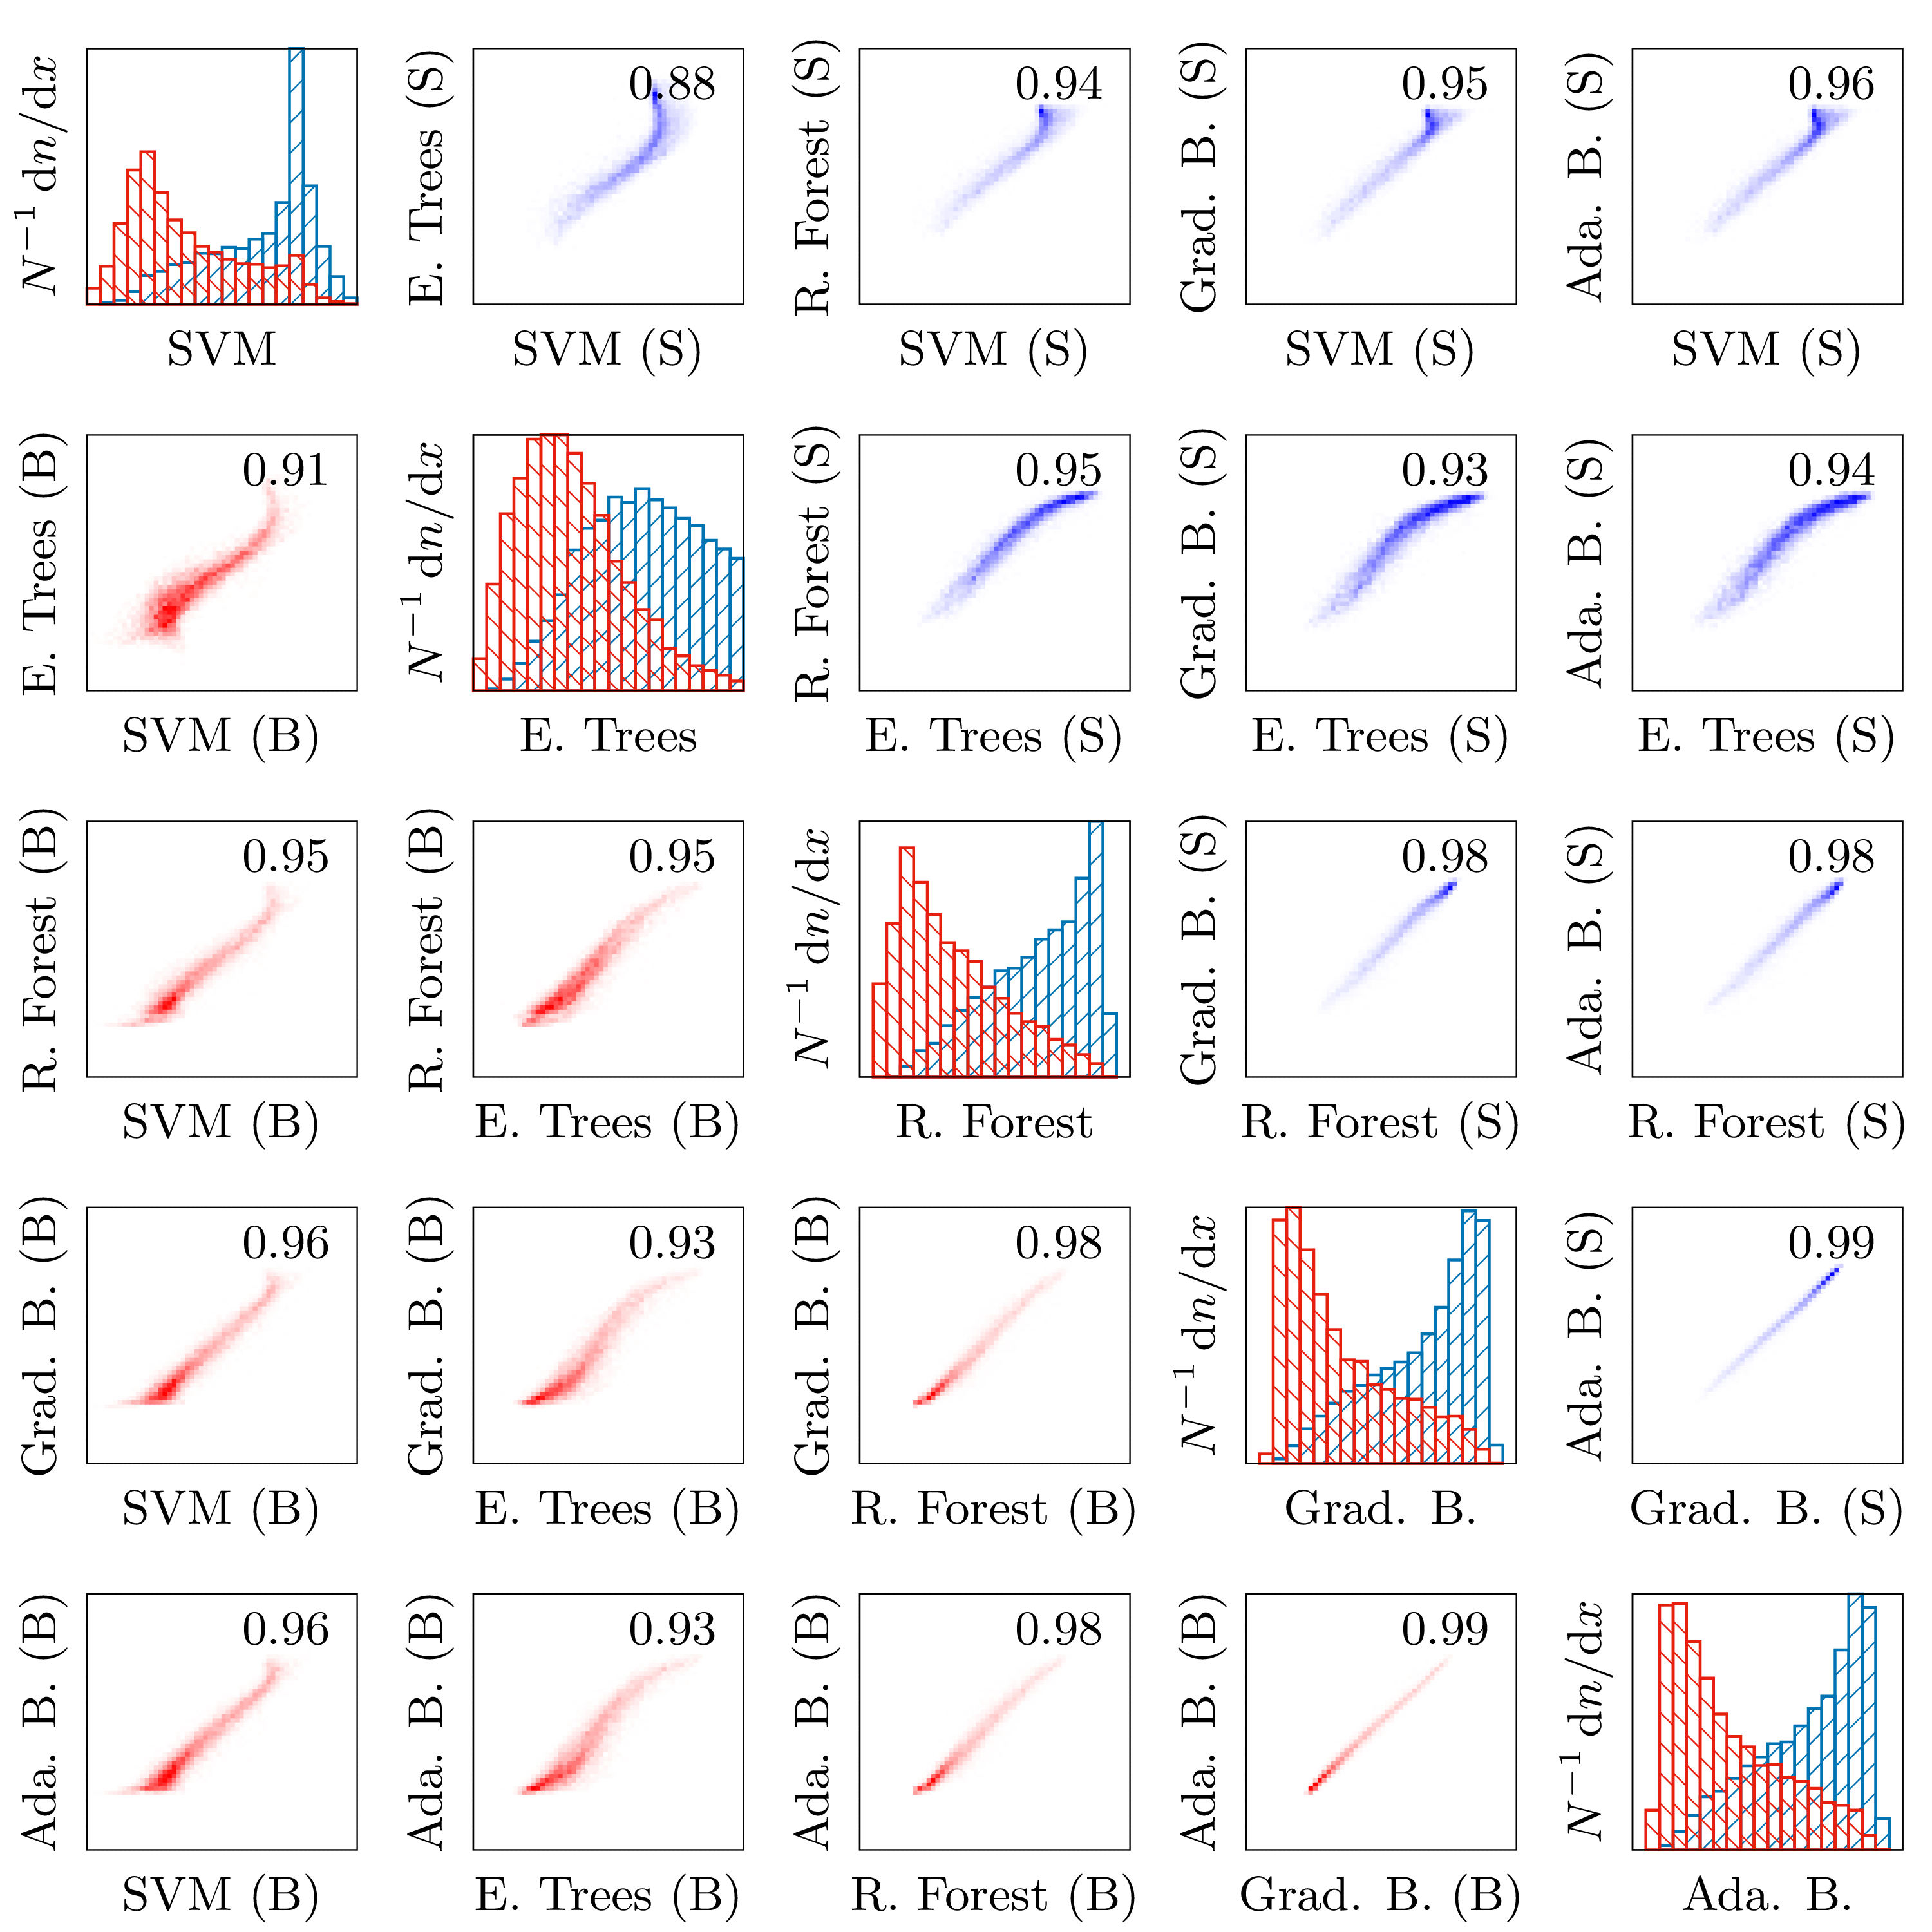
\includegraphics[height=.9\textheight]{mvaLz/stack_features_DD}\\
            (track type \textbf{DD})
        \end{column}
    \end{columns}
\end{frame}

\begin{frame}{Example: \Lz classifier}
    \begin{columns}
        \begin{column}{.45\textwidth}
            \scalebox{1.2}{\Lz classifier}
            \begin{itemize}
                \item 5 features of $\{ \Lz \}$
                \item Separate classifiers for LL and \textbf{DD}
                \item Optimize hyper-parameters of \textcolor{vertexDarkRed}{5 classifiers} using grid search w.r.t.\ ROC-AUC\ftnt{} value
            \end{itemize}
        \end{column}
        \begin{column}{.5\textwidth}
            \centering
            \includegraphics[height=.9\textheight]{mvaLz/stack_pcafeatures_DD}\\
            (track type \textbf{DD})
        \end{column}
    \end{columns}
\end{frame}

\begin{frame}{Fusion of high level classifiers}
    \begin{columns}
        \begin{column}{.5\textwidth}
            \centering
            \includegraphics[height=.9\textheight]{mva/features_DD}\\
            (track type DD)
        \end{column}
        \begin{column}{.45\textwidth}
            \scalebox{1.2}{Fusion of high level classifiers}
            \begin{itemize}
                \item Optimize rectangular cut classifier (to avoid MC fidelity issues\ftntdagger)
                \item \ldots using classifier outputs as features
                \begin{enumerate}
                    \item \Lz classifier
                    \item \Lb-\Dz classifier
                    \item \texttt{ProbNNp}
                    \item \texttt{ProbNNk}
                    \item Decay tree fit
                \end{enumerate}
                \item (Compare rect.\ cut clf.\ eff.\ against decision tree\ftntdagger)
            \end{itemize}
        \end{column}
    \end{columns}
\end{frame}

\begin{frame}{Classifier fusion}
    \begin{columns}
        \begin{column}{.5\textwidth}
            \scalebox{1.2}{Optimize rect.\ cut clf.}
            \begin{itemize}
                \item Minimize FPR\ftnt{} at given TPR\ftnt\ftnt{}
                \item Numerically noisy: use simulated annealing for finding minimum 
                \item Set thresholds at TPR $\approx 50\,\%$ (LL) and TPR $\approx 30\,\%$ (DD)
                \item (Refine \textit{optimal} TPR with in a second, tight max.\ step only using $\Lz / \Lb$-$\Dz$ classifiers\ftntdagger)
            \end{itemize}
        \end{column}
        \begin{column}{.5\textwidth}
            \only<1>{\includegraphics[scale=1.]{mva/roc}}%
            \only<2>{\includegraphics[scale=1.]{mva/significance}}%
        \end{column}
    \end{columns}

    \vspace{5mm}

    \footnotesize
    \phantom{\ftnt}\ftnt FPR: \underline{f}alse \underline{p}ositive \underline{r}ate, \ie{}, genuine bkg.\ predicted as sig.\\
    \ftnt\ftnt TPR: \underline{t}rue \underline{p}ositive \underline{r}ate, \ie{}, genuine sig.\ predicted as sig.
\end{frame}

\chapter{The Normalization Channel \texorpdfstring{\decay{\Lb}{\Dz\proton\pim}}{Λb → Dpπ}}
\label{chap:norm}
A normalization channel should comprise two key characteristics: First, the decay topology should be as close as possible to the primary decay channel such that common uncertainties and biases cancel.
Secondly, the normalization channel should be well established, clean to extract and contribute to the error budget as little as possible.

Obvious candidates for the present analysis are \decay{\Lb}{\Dz\proton\pim}, \decay{\Lb}{\Lz\Kp\pim}, \decay{\Lb}{\jpsi\Lz} and \decay{\Bbar{}^0_{(\squark)}}{\Dzb\KS}.
Despite its large branching fraction and clean reconstruction, the \jpsi\Lz mode, in particular if the \jpsi is reconstructed in its dimuon mode, will differ strongly in its detector response and trigger signature and thus requires a careful study of the corresponding simulation fidelity of both modes and therefore is not an ideal candidate.
The branching fractions of the other modes, as reported by the \gls{pdg}, are
\begin{align*}
    \BR(\decay{\Lb}{\Dz\proton\pim}) &= (6.3 \pm 0.7) \times 10^{-4} \,, \\
    \BR(\decay{\Lb}{\Lz\Kp\pim}) &= (5.7 \pm 1.3) \times 10^{-6} \,, \\
    \BR(\decay{\Bd}{\Dzb\Kz}) &= (5.2 \pm 0.7) \times 10^{-5} \,, \\
    \BR(\decay{\Bs}{\Dzb\Kzb}) &= (4.3 \pm 0.9) \times 10^{-4} \,,
\end{align*}
which do not include the \bquark-hadron production fractions which themselves depend on the kinematics of the \bquark~quark~\cite{LHCb_bProdFrac_7,LHCb_bProdFrac_13}.
Further, only roughly half of the \Kz mesons decay as \KS and within a similar detector acceptance as \Lz baryons.\footnote{Neglecting small \CP{} violating corrections and assuming similar lifetimes of the \KS state and the \Lz baryon.}
The other part will most likely escape undetected.
Taking both effects into account qualifies \decay{\Lb}{\Dz\proton\pim} as the most efficient candidate.

The final states of the charmless three-body decay approximate the signature of \decay{\Lb}{\Dz\Lz} best, but this advantage is compensated by its small branching fraction and the noisy background (\cf{}~Ref.~\cite{LbToLzhh}).
We note that this valuation will likely change in the future and future experiments might rank charmless three-body decays as their most suitable normalization candidate if provided with a sufficiently large set of \Lb decays.

The listed \bquark-meson decays also have a long living $\PV^0$ particle in their decay chain.
During analysis, \decay{\KS}{\pip\pim} decays have to be grouped w.r.t.\ their track types \gls{LL} and \gls{DD}, similar to \decay{\Lz}{\proton\pim}.
On the one hand, this leverages the access to track type specific properties which could cancel partially in the branching ratio, on the other hand, splitting the data sample hampers the analysis and, even though \KS and \Lz are both $\PV^0$ particles, the final states \pip\pim and \proton\pim can cause different signatures in the \lhcb{} detector which make \Dz\proton\pim the better proxy for \Dz\Lz, especially for \gls{LL} tracks.
At the same time, the fidelity of \gls{mc} simulated \Lb decays is known for being imperfect, especially in terms of kinematic distributions.
Using \Lb decays in the primary decay, as well as the normalization mode minimizes this uncertainty source in the branching fraction.

Considering the listed arguments, we use \decay{\Lb}{\Dz\proton\pim} as the normalization mode.
We will briefly discuss the decay in Sec.~\ref{sec:LbToDzppi_thedecay} and will then outline the selection strategy.
In Sec.~\ref{sec:LbToDzppi_yields} we will then extract signal yields which we will use later for determining the branching fraction.

\section{The Decay \texorpdfstring{\decay{\Lb}{\Dz\proton\pim}}{Λb → Dpπ}}
\label{sec:LbToDzppi_thedecay}
The decay \decay{\Lb}{\Dz\proton\pim} is a high statistics channel and leveraged the discovery of the \Lb baryon in 1981 \cite{Lbdisc}.
The final states are the same as in \decay{\Lb}{\Dz\Lz} but due to the different quark transitions, it is much less susceptible for \CP violation.\footnote{Changing the pion to a kaon reduces the branching fraction by a factor of $\lambda^2$ (\gls{wolfenstein}) but now allows an effective extraction of the \gls{ckm} phase $\gamma$ (\cf{} Sec.~\ref{sec:lbcpv}).} 
The large branching fraction gives a good signal to background ratio after applying simple rectangular selection requirements.
Rather than optimizing these selection requirements for \decay{\Lb}{\Dz\proton\pim}, the opulent signal to background ratio allows the use of a subset of the optimized requirements for the primary decay \decay{\Lb}{\Dz\Lz} with some minor corrections. 
These selections are split into a preselection and a loose selection part which are outlined in the following sections.

\subsection{Preselection}
We use the full recorded data set of \gls{runtwo} and the \gls{stripping} versions listed in Tab.~\ref{tab:LbToDzLz_vstripping}.
Despite their different naming, the selection requirements vary slightly.
These differences are compensated by adopting the tightest selection requirement among conflicting values if necessary.

\begin{table}[htbp]
    \centering
    \caption{\Gls{stripping} and Reco versions used for reconstructing \decay{\Lb}{\Dz\proton\pim}.}
    \label{tab:LbToDzppi_vstripping}

    \begin{tabular}{lll}
        \toprule
        Year & \Gls{stripping} & Reco \\
        \midrule
        2015 & \texttt{24r1} & \texttt{15a} \\
        2016 & \texttt{28r1} & \texttt{16} \\
        2017 & \texttt{29r2} & \texttt{17} \\
        2018 & \texttt{34} & \texttt{18} \\
        \bottomrule
    \end{tabular}
\end{table}

All selection criteria of the preselection step are listed in Tab.~\ref{tab:LbToDzppi_stripsel} where we use the same nomenclature that we introduced in Sec.~\ref{sec:LbToJpsiLz_presel}.
Additionally, at least one \gls{hlt} trigger flag among \texttt{Hlt2.*IncPhi.*Decision} or \texttt{Hlt2Topo.*Decision} is required, \cf{}~Refs.~\cite{triggerRun2,HTL2TopoLines} for more detailed information.

\subsection{Loose Selection}
\label{sec:LbToDzppi_loosesel}
Similar to the previous analyses of \decay{\Lb}{\jpsi\Lz} and \decay{\Lb}{\Dz\Lz} decays, we select only events corresponding to the best \gls{pv} hypothesis for the following steps.
All selection criteria of the loose selection are shown in Tab.~\ref{tab:LbToDzppi_loosesel} and are grouped into five categories.
Again, categories~1 to 4 are the same that we used and described previously in Sec.~\ref{sec:LbToJpsiLz_loosesel} and Sec.~\ref{sec:LbToDzLz_loosesel}.
The purpose of selection requirements of category~5 is to reject physical backgrounds such as \decay{\Bd}{\Dzb\pip\pim}, \decay{\Bd}{\Dzb\Km\pip} or \decay{\Bs}{\Dzb\Km\pip} and \decay{\Lb}{\Dz\proton\Km} by requiring a minimal threshold w.r.t.\ $\texttt{ProbNNp}(\proton)$ and a veto against large values of $\texttt{ProbNNk}(\pion)$, respectively.
Since most of the charge tracks in an event are caused by genuine pions, the former selection requirement also helps to suppress combinatorial background (category~1).
The combined efficiency for \gls{mc} simulated events is $71.10(25)\,\%$ where the uncertainty only takes statistical fluctuations into account (\cf{}~Sec.~\ref{sec:LbToDzLz_loosesel}).

\begin{table}[htbp]
    \caption{Selection criteria of loose selection used for reconstructing \decay{\Lb}{\Dz\proton\pim}. The selections are grouped into four categories which are explained in Sec.~\ref{sec:LbToDzppi_loosesel}.}
    \label{tab:LbToDzppi_loosesel}
    \centering
    \begin{tabular}{llc}
        \toprule
        Particle & Selection & Category \\
        \midrule
        \pion & $3 \le p \le 150\,$\gevc & 1 \\
        \kaon & $3 \le p \le 150\,$\gevc & 1 \\
        \proton & $9 \le p \le 150\,$\gevc & 1 \\
        \proton & \texttt{ProbNNp} $\ge 0.2$ & 1, 5 \\
        \pi & \texttt{ProbNNk} $\le 0.3$ & 5 \\
        \midrule
        \Dz & $0 \le$ FD sig. $\le 100$ & 1 \\
        \Dz & \dchisqip w.r.t.\ best \gls{pv} $\ge 5$ & 1 \\
        \midrule
        \Lb & \dchisqip w.r.t.\ best \gls{pv} $\le 25$ & 1 \\
        \Lb & $5 \le m \le 6\,\gevcc$ & 3 \\
        \Lb & $2 \le \eta \le 4.5$ & 4 \\
        \Lb & $\pt \le 20\,\gevc$ & 4 \\
        \midrule
        \Lb & $\exists$ converged \gls{dtf} & 1 \\
        \Lb & $\chi_\mathrm{DTF}^2 / \text{\gls{dof}} \le 10$ & 1 \\
        \bottomrule
    \end{tabular}
\end{table}

\subsection{Calibration}
\label{sec:norm_calibration}
Three-body decays typically have resonances among their final states, whereas in two-body decays the only possible resonance is the mother of the decay chain itself.
In particular, \decay{\Lb}{\Dz\proton\pim} decays have a rich set of resonances among \Dz\proton and \Dz\pim pairs~\cite{LbToDzphAndLch}.
These resonances are not taken into account during the generation of the \gls{mc} simulated decays.
Instead, the decays are simulated flat in the so-called \textit{square Dalitz plot} (\cf{} Refs.~\cite{dalitz1,dalitz2} and in particular Ref.~\cite{BsToDKpi} for the definition of a square Dalitz plot).
In order to make recorded data and \gls{mc} simulated event comparable we calibrate the former by assigning weights to each event.\footnote{Technically, the parameters $m'$ and $\theta'$ (\cf{}~Ref.~\cite{BsToDKpi}), are evaluated with a \Gls{dtf} where all intermediate particle masses (\ie{}, including $m(\Lb)$ itself) are constrained to increase the resolution of the Dalitz distribution.}
The weights are the inverted values of the (normalized) smoothed square Dalitz plot profile, where the smoothing is performed in bins using a $5 \times 5$ kernel function
\begin{equation*}
    \mathcal{K} = \begin{pmatrix}
        0 & 0 & 1 & 0 & 0 \\
        0 & 2 & 2 & 2 & 0 \\
        1 & 2 & 5 & 2 & 1 \\
        0 & 2 & 2 & 2 & 0 \\
        0 & 0 & 1 & 0 & 0
    \end{pmatrix}.
\end{equation*}
The smoothed profile is the result of a convolution with $\mathcal{K}$ and a subsequent normalization where kernel pixels that extends past the boundary are set to zero (Kernel Crop).
Below, we apply this efficiency correction to recorded data after the respective selection steps but suppress an explicit mention for the sake of brevity.
As a consequence, we also use (binned) weighted minimum $\chi^2$-fits in the following instead of a (single entry) maximum likelihood method.
Calibrating the recorded data changes the shapes of the physical background, whereas the impact on the fitted signal yields is less than $14\,\%$.

\section{Yield Extraction}
\label{sec:LbToDzppi_yields}
The distribution of the invariant mass $m(\Dz\proton\pim)$ after applying the loose selection requirements is shown in Fig.~\ref{fig:LbToDzppi_mLb_nocuts}.
\begin{figure}[htbp]
    \centering
    \includegraphics[scale=1.]{Lb2Dzppi_mvaxcheck/mLb_nocuts.png}
    \caption{Invariant mass distribution of \Dz, \proton and \pim candidates after applying the loose selection requirements. The regions I and III are used for extracting the shape of the combinatorial background. Region II indicates the signal region that is used for extracting the signal yield. The dashed line indicate the fitted shape of the combinatorial background.}
    \label{fig:LbToDzppi_mLb_nocuts}
\end{figure}
An exhaustive fit model that comprises a precise signal model, as well as all background components such as partially reconstructed \decay{\Lb}{\Dstarz\proton\pim} (large enhancement between $5.3\,\gevcc$ and $5.5\,\gevcc$) or \glspl{reflection} from \decay{\Lb}{\Dz\proton\Km} decays or other \Bd and \Bs decays requires a thorough analysis of all these components, \cf{}~Ref.~\cite{LbToDzphAndLch}.
For the present analysis we find that a simple yet flexible fit model suffices, while not contributing to the overall error budget excessively.
Within this fit model, the signal region is limited tightly to $5.58 \le m(\Dz\proton\pim) \le 5.66\,\gevcc$ (region II in Fig.~\ref{fig:LbToDzppi_mLb_nocuts}) and thus reduces the impact of physical background contribution, in particular of \glspl{reflection} below $m(\Lb)$.
The shape of the combinatorial background is parametrized with the exponential function given in Eq.~\eqref{eq:apdx_pdfs_exprel2} and is extracted from a lower sideband $5.2 \le m(\Dz\proton\pim) \le 5.3\,\gevcc$ and an upper sideband $5.7 \le m(\Dz\proton\pim) \le 6\,\gevcc$, referred to as region I and III in Fig.~\ref{fig:LbToDzppi_mLb_nocuts}.
The signal yield is obtained by extrapolating the fitted background \gls{pdf} into region~II, scaling with the number of events in regions~I and III, and subtracting the result from the number of events in region~II.
Applying this fitting strategy to the distribution of the invariant mass $m(\Dz\proton\pim)$ after the loose selection, as shown in Fig.~\ref{fig:LbToDzppi_mLb_nocuts}, yields $7.04(6) \times 10^4$ signal events where the uncertainty only takes statistical fluctuations into account.
In order to estimate the systematic uncertainty we use the same fitting strategy to extract the yields from two further reduced samples, where the former (latter) sample is obtained by requiring $\texttt{ProbNNk} \ge 0.3$ ($0.57$) for the kaon and a \gls{dtf} probability above $0.01$.
The thresholds of the selection requirements w.r.t.\ the \texttt{ProbNNk} responses are the optimized values for \gls{LL} and \gls{DD} tracks that we found for the \decay{\Lb}{\Dz\Lz} decay in Chap.~\ref{chap:mva}, whereas the threshold w.r.t.\ the \gls{dtf} probability is chosen ad hoc and proven to significantly improve the signal to background ratio.
Both samples are shown in Fig.~\ref{fig:LbToDzppi_hLbM_no_clf}.
\begin{figure}[htbp]
    \centering
    \begin{subfigure}{.49\textwidth}
        \centering
        \includegraphics[scale=1.]{Lb2Dzppi_mvaxcheck/hLbM_LL_no_clf.png}
    \end{subfigure}
    \begin{subfigure}{.49\textwidth}
        \centering
        \includegraphics[scale=1.]{Lb2Dzppi_mvaxcheck/hLbM_DD_no_clf.png}
    \end{subfigure}
    \caption{Combined invariant mass distributions of \Dz, \proton and \pim candidates, as well as the fit of the combinatorial background (dashed line). The distributions are the result of a set of selection criteria that resembles part of the tight selection for \gls{LL} (left) and \gls{DD} (right) \decay{\Lb}{\Dz\Lz} decays.}
    \label{fig:LbToDzppi_hLbM_no_clf}
\end{figure}

Requiring both of these selection criteria results in a cleaner data sample but also unveils a bias of the fit model at the lower tail of the \Lb signal peak.
The fitted yields of these two fits are shown in Tab.~\ref{tab:LbToDzppi_xcheckN}.
Applying the very same fitting strategy to \gls{mc} simulated events gives access to the (\gls{mc} predicted) efficiency of the required selection and allows the extrapolation to the total amount of events before requiring the selection.
Both of these extrapolated numbers should match the number we found with our first fit.
The deviation is an admixture of deviations due to fidelity issues of the \gls{mc} simulated events and an overestimation of the signal yield due to a bias of the fitting model.
A conservative approach to approximate the systematic uncertainty of the fit is to ignore the former part and take the entire deviation between the three fitted yields as an upper limit of the uncertainty interval,
\begin{equation*}
    n = 7.0(5) \times 10^4 \,.
\end{equation*}
The uncertainty corresponds to a relative uncertainty of $7\,\%$ which is sufficient for the sake of the present analysis.
As stated, this approximation is conservative and renders additional studies, such as the unfolding of the strongly correlated systematic uncertainties of the three samples, unnecessary.
\begin{table}[htbp]
    \centering
    \caption{Efficiencies of applying additional selection criteria (\gls{LL}~sel.) and (\gls{DD}~sel.) on top of the loose selection of \decay{\Lb}{\Dz\proton\pim} decays, evaluated by fitting \gls{mc} simulated events. These efficiencies are then used to extrapolate (ext.) the fitted yields (fit~2) of recorded data and compared with the fitted yield (fit~1) of the respective distribution after requiring only the loose selection.}
    \label{tab:LbToDzppi_xcheckN}
    \begin{tabular}{lll}
        \toprule
        & \multicolumn{1}{c}{\gls{LL} sel.} & \multicolumn{1}{c}{\gls{DD} sel.} \\
        \midrule
        %MC efficiency & $77.009(34)\,\%$ & $71.77(4)\,\%$ \\
        %ec.\ data (fit 2) & $5.776(34) \times 10^4$ & $5.282(32) \times 10^4$ \\
        %ec.\ data (ext.) & $7.50(4) \times 10^4$ & $7.36(4) \times 10^4$ \\
        \gls{mc} efficiency & $77.020(34)\,\%$ & $71.70(4)\,\%$ \\
        Rec.\ data (fit 2) & $5.746(34) \times 10^4$ & $5.301(32) \times 10^4$ \\
        Rec.\ data (ext.) & $7.45(4) \times 10^4$ & $7.39(4) \times 10^4$ \\
        \midrule
        %Rec.\ data (fit 1) & \multicolumn{2}{c}{{$7.07(6) \times 10^4$}} \\
        Rec.\ data (fit 1) & \multicolumn{2}{c}{{$7.04(6) \times 10^4$}} \\
        \bottomrule
    \end{tabular}
\end{table}

In Chap.~\ref{chap:br} we argue that only events with a positive \gls{lzero} \gls{tis} trigger decision are needed for the normalization of the branching ratio.
The corresponding distributions of the invariant mass $m(\Dz\proton\pim)$ and the respective fits for recorded data are shown in Fig.~\ref{fig:LbToDzppi_hLbM_no_clf_tis}.
The fits yield (including our $7\,\%$ uncertainty estimation) $n = 3.93(28) \times 10^4$ and $n = 3.60(25) \times 10^4$ for the \gls{LL} and \gls{DD} selection, respectively.
\begin{figure}[htbp]
    \centering
    \begin{subfigure}{.49\textwidth}
        \centering
        \includegraphics[scale=1.]{br/hLbM_LL_no_clf_tis.png}
    \end{subfigure}
    \begin{subfigure}{.49\textwidth}
        \centering
        \includegraphics[scale=1.]{br/hLbM_DD_no_clf_tis.png}
    \end{subfigure}
    \caption{Combined invariant mass of \Dz, \proton and \pim candidates from recorded data. The selection criteria resembles parts of the tight selection for \gls{LL} (left) and \gls{DD} \decay{\Lb}{\Dz\Lz} decays. Additionally, the \gls{lzero} \gls{tis} trigger is required.}
    \label{fig:LbToDzppi_hLbM_no_clf_tis}
\end{figure}


\chapter{Physical Backgrounds}
\label{chap:bkgs}
\chapquote{Today's prediction is tomorrow's prior.}{Glen Cowan, during TAE summer school 2017}
Regarding G.~Cowan's quote about tomorrow's prior, decays that were first observed during \gls{runone}, such as $\decay{\Lb}{\Lz\Ph\Ph'}$ and \decay{\Bsb}{\Dz\KS} not only have become today's prior, they already have to be considered as background candidates in \gls{runtwo} analyses.
In this section we discuss those and other physical background contributions which we separate into non-resonant backgrounds (Sec.~\ref{sec:bkgs_nonres}), partially reconstructed backgrounds (Sec.~\ref{sec:bkgs_part}), and \glspl{reflection} (Sec.~\ref{sec:bkgs_refl}).
While we find that most background contributions can be neglected due to a sufficiently strong suppression, partially reconstructed decays including \Dstarz resonances or \Sz baryons, stay a nuisance and enter the fit model of the subsequent $m(\Dz\Lz)$ fit.

\section{Non-Resonant Background}
\label{sec:bkgs_nonres}
\decay{\Lb}{\Dz\proton\pim} decays have the potential of being a dangerous (non-resonant) background for the \decay{\Lb}{\Dz\Lz} mode, if the \Lz daughters are reconstructed as \gls{LL} tracks.
If not sufficiently suppressed, this background is irreducible in the $m(\Dz\Lz)$ distribution and very hard to unfold from genuine \decay{\Lb}{\Dz\Lz} decays by conventional fitting approaches.
Luckily for the present analysis, the kinematic suppression of the \gls{stripping} phase already gives a strong suppression,\footnote{Mostly due to the required finite mass window around $m(\Lz)$.} as shown in Chap.~\ref{chap:stripeff}.
Applying the dedicated tight \decay{\Lb}{\Dz\Lz} selection (\cf{}~Sec.~\ref{sec:LbToDzLz_tightsel}) gives an additional suppression and accepts \num{65} of \num{46740} (weighted) events, where the latter is the amount of events that already pass the dedicated pre- and loose \decay{\Lb}{\Dz\Lz} selection steps.\footnote{Technically, we use so-called \textit{filtered} events for this task. Filtered events give larger yields but estimating the combined reconstruction and \gls{stripping} efficiency is more challenging than for ordinary simulated events (which we used for the latter task).}
A 95\,\% confidence interval of the corresponding efficiency is $[1.1 \ldots 1.8]\,\times 10^{-3}$.
The efficiencies of each selection step individually, without requiring any of the other criteria, are shown in Tab.~\ref{tab:LbToDzppi_bkg_tightseleffs}.
\begin{table}[htbp]
    \centering
    \caption{Efficiencies of applying the tight selection criteria as found in Sec.~\ref{sec:LbToDzLz_tightsel} of the \decay{\Lb}{\Dz\Lz} selection to genuine \decay{\Lb}{\Dz\proton\pim} decays, evaluated with \gls{mc} simulated events.}
    \label{tab:LbToDzppi_bkg_tightseleffs}
    \begin{tabular}{lS[separate-uncertainty=false]}
        \toprule
        Selection criterion & {Efficiency [\%]} \\
        \midrule
        \Lz Clf. $\ge 0.67$ & 4.68 \pm 0.10 \\
        \Lb-\Dz Clf. $\ge 0.73$ & 19.26 \pm 0.18 \\
        \texttt{ProbNNp} $\ge 0.6$ & 22.87 \pm 0.19 \\
        \texttt{ProbNNk} $\ge 0.3$ & 23.35 \pm 0.20 \\
        \Gls{dtf} prob. $\ge 0.012$ & 0.61 \pm 0.04 \\
        \midrule
        Combination & 0.139 \pm 0.017 \\
        \bottomrule
    \end{tabular}
\end{table}
Combining this efficiency with the suppression factor of the \gls{stripping} phase leverages the estimation of an upper limit of the accumulated probability $P$ of seeing at most $n$ genuine \decay{\Lb}{\Dz\proton\pim} events in the invariant mass of \Dz and \Lz candidates:
\begin{equation*}
    P = \sum_{k=0}^n \begin{pmatrix} N \\ k \end{pmatrix} p^k (1-p)^{N-k} \,.
\end{equation*}
In Fig.~\ref{fig:LbToDzppi_bkg_efflimit} we show the accumulated probability for $p=9 \times 10^{-5}$ (dashed line) which corresponds to a conservative approximation of both factors.
\begin{figure}[htbp]
    \centering
    \includegraphics[scale=1.]{Lb2Dzppi_bkg/binom_prob_acc.png}
    \caption{Probability of seeing more than $n$ genuine \decay{\Lb}{\Dz\proton\pim} decays in $m(\Dz\Lz)$. The solid (dashed) line corresponds to our choice of selection steps, including (excluding) the additional selection requirements w.r.t.\ $m(\proton\pim)$ and the \Lz flight distance significance.}
    \label{fig:LbToDzppi_bkg_efflimit}
\end{figure}
We argue that this suppression on its own is not sufficient.
In the following we will therefore tighten the mass window of $m(\proton\pim)$ around $m(\Lz)$ and establish a veto against small values of the \Lz flight distance significance.
These additional requirements decrease the combined efficiency to at most $p=8 \times 10^{-6}$ at a 95\,\% CL (solid line in Fig.~\ref{fig:LbToDzppi_bkg_efflimit}), corresponding to a probability of seeing not more than three events above $99\,\%$.

\begin{figure}[htbp]
    \centering
    \begin{subfigure}{.49\textwidth}
        \centering
        \includegraphics[scale=1.]{Lb2Dzppi_bkg/mLz_loose.png}
    \end{subfigure}
    \begin{subfigure}{.49\textwidth}
        \centering
        \includegraphics[scale=1.]{Lb2Dzppi_bkg/mLz.png}
    \end{subfigure}
    \caption{Combined invariant mass of \proton and \pim candidates of simulated \decay{\Lb}{\Dz\proton\pim} decays, reconstructed and fitted via a \gls{dtf} as \decay{\Lb}{\Dz\Lz}. The loose selection (left) and tight selection (right) are the dedicated \decay{\Lb}{\Dz\Lz} selections as described in Sec.~\ref{sec:LbToDzLz_prepro}.}
    \label{fig:LbToDzppi_bkg/mLz}
\end{figure}
In Fig.~\ref{fig:LbToDzppi_bkg/mLz} we show the invariant mass distribution of $m(\proton\pim)$ before and after applying the dedicated \decay{\Lb}{\Dz\Lz} tight selection.
Apparently, it is not flat but strongly (asymmetrically) suppressed for $m(\proton\pim)>m(\Lz)$.
We find that this structure is introduced by requiring a minimum flight distance (\cf{}~Sec.~\ref{sec:LbToDzLz_loosesel}) and simultaneously constraining the \Lz mass in a \gls{dtf} (\cf{} Appx.~\ref{chap:apdx_dtf} for a more detailed description of this correlation.)
We choose
\begin{align*}
    m(\proton\pim) - m(\Lz_\text{PDG}) &\overset{!}{>} -4\mev \,, \\
    \text{\Lz FD sig.} &\overset{!}{>} 25 \,,
\end{align*}
where $m(\Lz_\text{PDG})$ is taken from Ref.~\cite{pdg},
as thresholds for $m(\proton\pim)$ and the flight distance significance of the \Lz baryon which leaves, when applied in combination, only one event left (weight $1.12$).
In Fig.~\ref{fig:Lb2Dzppi_bkg_fdsig_cdf} we show the cumulative distribution of the latter in combination with and without the tight selection.
With $n<2$ and a preselection suppression factor of $20$ this corresponds to an 95\,\% confidence interval of $[0.26 \ldots 8]\,\times 10^{-6}$.
\begin{figure}[htbp]
    \centering
    \includegraphics[scale=1.]{Lb2Dzppi_bkg/fdsig_cdf.png}
    \caption{Cumulative distribution of selections w.r.t.\ the flight distance significance of the (spurious) \Lz candidates from \decay{\Lb}{\Dz\proton\pim} decays after (solid line) and before (dashed line) applying the dedicated tight \decay{\Lb}{\Dz\Lz} selection.}
    \label{fig:Lb2Dzppi_bkg_fdsig_cdf}
\end{figure}

We refer to Ref.~\cite{LbToDzphAndLch} for studies of Dalitz plots of \decay{\Lb}{\Dz\proton\pim} decays and note that the \Lz baryon is located at low values of $m^2_{\proton\pion}$ and large values of $m^2_{\PD\proton}$.
Both areas show no large resonance structures and thus support the conservative trait of our approximation.

\section{Partially Reconstructed Backgrounds}
\label{sec:bkgs_part}
In the present analysis partially reconstructed backgrounds come from intermediate states that decay to either a soft photon or a soft neutral pion.
These low energetic particles typically escape undetected at \lhcb and thus making the respective backgrounds irreducible.
In particular, we will consider \decay{\Lb/\Xibz}{\Dz\Sz} and \decay{\Xibz}{\Dz\Xiz} decays, as well as \decay{\Lb/\Xibz}{\Dstarz\Lz}, where in the former cases the \Pgamma (\piz) from \decay{\Sz}{\Lz\Pgamma} (\decay{\Xiz}{\Lz\piz}), and in the latter case the \Pgamma (\piz) from \decay{\Dstarz}{\Dz\Pgamma} (\decay{\Dstarz}{\Dz\piz}) is lost.
We devoted the entire Sec.~\ref{sec:isospin} of our theory part to the discussion of the irreducible \decay{\Sz}{\Lz\Pgamma} background.
In addition we analyze its kinematics, as well as the kinematics of the other partially reconstructed background sources in depth in Appx.~\ref{chap:apdx_partbkg}.
Since these backgrounds are irreducible we will encounter them in our fitting model.

\section{Reflections}
\label{sec:bkgs_refl}
Apart from random track combinations, non-resonant and partially reconstructed decays, so-called \textit{\glspl{reflection}} potentially contaminate the signal region in the invariant mass distribution $m(\Dz\Lz)$.
\Glspl{reflection} are fully reconstructed decays where a spurious mass hypothesis was assigned to at least one of the particles within the respective decay chain.
Since reconstruction is typically performed in the upstream direction of the respective decay chain, this wrong assignment also propagates as a shift and dilution of the mass distributions.
Decays, such as \decay{\Bsb}{\Dz\KS}, can contaminate the signal region if the kaon decay \decay{\KS}{\pip\pim} becomes a \gls{reflection} by misidentifying the \pip as a proton and thus fakes a \decay{\Lz}{\proton\pim} decay.
This smears the invariant mass distribution of the \KS, as well as the \Bs meson mass distribution and consequently introduces background contributions to the invariant mass distribution $m(\Dz\Lz)$.

For a given $n$-body decay the invariant mass of the mother $M$ is given by the invariant masses $m_i$ and three-momenta $\vec{p}_i$ of the daughters via the relation
\begin{equation*}
    M^2 = \left( \sum_{i=1}^n \sqrt{m_i^2 + \vec{p}_i^{\,2}} \right)^2 - \left( \sum_{i=1}^n \vec{p}_i \right)^2 \,.
\end{equation*}
The shift of $M$ in case of a spurious mass hypothesis $m_j \to m_j + \delta m_j$ is non-linear in $\delta m_j$ and depends on the respective momenta, hence the transformation of the invariant mass distributions due to \glspl{reflection} is non-trivial and depend on the momentum distributions.

In the following we discuss the two main sources of \glspl{reflection} in the present analysis.
In Sec.~\ref{sec:bkgs_charmless} we study charmless three-body decays and then discuss the possible contamination of genuine \KS decays in Sec.~\ref{sec:bkgs_ks}.
Both background candidates are eventually found to be negligible given the amount of available statistics after applying the dedicated tight \decay{\Lb}{\Dz\Lz} selection and are thus not included in the subsequent $m(\Dz\Lz)$ fit model.

\subsection{Charmless Decays}
\label{sec:bkgs_charmless}
Charmless three-body decays $\decay{\Lb/\Xibz}{\Lz\Ph\Ph'}$ are a nuisance in searches for \CP violation in \decay{\Lb}{\Dz\Lz} decays when $\Ph\Ph'$ are spuriously reconstructed as $\decay{\Dz}{\Ph\Ph'}$.
The reported branching fractions are (\cf{}~Refs.~\cite{pdg,LbToLzhh})
\begin{align*}
    \BR(\decay{\Lb}{\Lz\Kp\Km}) &= (1.62 \pm 0.23) \times 10^{-5} \,, \\
    \BR(\decay{\Lb}{\Lz\Kp\pim}) &= (5.7 \pm 1.3) \times 10^{-6} \,, \\
    \BR(\decay{\Lb}{\Lz\pip\pim}) &= (4.7 \pm 1.9) \times 10^{-6} \,, 
\end{align*}
and thus will appear as physical background in the relevant \gls{ads} and \gls{glw} modes.
Similarly, \decay{\Xibz}{\Lz\Kp\Km}, \decay{\Xibz}{\Lz\Km\pip} and \decay{\Xibz}{\pip\pim} decays are background candidates in \decay{\Xibz}{\Dz\Lz} analyses.
All these modes are hard to control and require decent statistics to, for example, estimate their contribution to the signal yields by analyzing the combined invariant masses of \Dz and \Lz candidates in slices of the \Dz flight distance.
Beneficially for the present analysis, the \decay{\Lb}{\Lz\Km\pip} decay is suppressed w.r.t.\ \decay{\Lb}{\Lz\Kp\pim} with at least a factor of a box diagram and neither \decay{\Lb}{\Lz\Km\pip}, nor \decay{\Xibz}{\Lz\Km\pip} were observed experimentally at the time of writing.

For the present analysis where we reconstruct the \Dz meson as \decay{\Dz}{\Km\pip}, the \decay{\Lb}{\Lz\Kp\Km} background only enters indirectly via \gls{reflection}.
Below, we show that we can suppress the contribution coming from \decay{\Lb}{\Lz\Kp\Km} decays (largest branching fraction) sufficiently and thus renders dedicated analyses of the remaining \decay{\Lb}{\Lz\Ph\Ph'} modes unnecessary.
We use weighted, \gls{truthmatched} \gls{mc} simulated events\footnote{Generated flat in phase space.} for this task where we rely on the established weights without adding acceptance corrections due to the limited dataset.

First, we apply the dedicated \decay{\Lb}{\Dz\Lz} preselection step with the tightened requirements we established in Sec.~\ref{sec:bkgs_nonres} which already greatly reduces the \decay{\Lb}{\Lz\Kp\Km} data set from \num{2875} to \num{570} and \num{7055} to \num{1785} events\footnote{The reduced numbers are the accumulated weights of the \gls{mc} simulated events.} for \gls{LL} and \gls{DD} tracks, respectively.\footnote{This strong suppression is driven by the fact that the dedicated \decay{\Lb}{\Dz\Lz} preselection step already includes requirements w.r.t.\ the fit probability, \Dz flight distance, etc.}
Secondly, we apply the selection steps w.r.t.\ the \gls{dtf} probability, and the responses of the \texttt{ProbNNp} and \texttt{ProbNNk} classifiers for the \proton and \Km, respectively.
The corresponding efficiencies are listed in Tab.~\ref{tab:bkgs_charmless_nonclfeff}.
The efficiencies for the selection requirements w.r.t.\ \texttt{ProbNNp} and \texttt{ProbNNk} are compatible with those we found for genuine \decay{\Lb}{\Dz\Lz} decays, whereas the \gls{dtf} reveals its strong separation power due to the \Dz mass constraint.
\begin{table}[htbp]
    \centering
    \caption{Efficiencies of the dedicated \decay{\Lb}{\Dz\Lz} tight selection requirements when applied to \decay{\Lb}{\Lz\Kp\Km}, reconstructed as \decay{\Lb}{\Dz\Lz}, and genuine \decay{\Lb}{\Dz\Lz} decays. The efficiencies are obtained from weighted \gls{mc} simulated events.}
    \label{tab:bkgs_charmless_nonclfeff}
    \begin{tabular}{l%
                    S[separate-uncertainty=false,table-format=2.2(2)]%
                    S[separate-uncertainty=false,table-format=2.2(2)]%
                    S[separate-uncertainty=false,table-format=2.2(2)]%
                    S[separate-uncertainty=false,table-format=2.2(2)]}
        \toprule
        & \multicolumn{2}{c}{{\decay{\Lb}{\Lz\Kp\Km}}} & \multicolumn{2}{c}{{\decay{\Lb}{\Dz\Lz}}} \\
        & {\gls{LL} [\%]} & {\gls{DD} [\%]} & {\gls{LL} [\%]} & {\gls{DD} [\%]} \\
        \midrule
        \Gls{dtf} prob. & 43.5 \pm 2.1 & 28.1 \pm 1.1 & 89.16 \pm 0.31 & 82.07 \pm 0.24 \\
        $\texttt{ProbNNp}(\proton)$ & 94.2 \pm 1.0 & 86.6 \pm 0.8 & 92.87 \pm 0.26 & 81.54 \pm 0.25 \\
        $\texttt{ProbNNk}(\kaon)$ & 91.3 \pm 1.2 & 84.7 \pm 0.9 & 92.51 \pm 0.26 & 84.50 \pm 0.23 \\
        \midrule
        Combination & 26.4 \pm 1.8 & 24.9 \pm 1.0 & 88.51 \pm 0.32 & 88.67 \pm 0.20 \\
        \bottomrule 
    \end{tabular}
\end{table}

The efficiencies of applying the \Lz and \Lb-\Dz classifier selection requirements are estimated after applying all previous discussed selections and are listed in Tab.~\ref{tab:bkg_charmless_clfeff}.
Interestingly, both classifiers show a strong separation power, except for the \Lz classifier when applied to \gls{LL} tracks.
In order to understand this behavior we train \glspl{svm} on the reduced data set using all pairwise combinations of two features to estimate each feature importance.
For the \Lb-\Dz classifier we find that almost the entire separation power stems from the \Dz flight distance feature.
This is expected, since in the case of genuine \decay{\Lb}{\Lz\Kp\Km} decays, the fitted flight distance of the \Kp\Km pair is smaller on average than for genuine \Dz meson.
More surprisingly, the \Lz classifier is also capable to separate between genuine \decay{\Lb}{\Dz\Lz} and \decay{\Lb}{\Lz\Kp\Km} decays.
The rather large deviation for \gls{LL} and \gls{DD} tracks is rooted in the mild thresholds of the former but adjusts when the thresholds are raised.
Using the same technique we used previously, we find that the separation power is driven by deviations in the \pt distributions which we discuss in detail in Appx.~\ref{sec:apdx_charmlessrel_Lzp}.
\begin{table}[htbp]
    \centering
    \caption{Efficiencies of the optimized \decay{\Lb}{\Dz\Lz} tight selection requirements when applied to \decay{\Lb}{\Lz\Kp\Km}, reconstructed as \decay{\Lb}{\Dz\Lz}, and genuine \decay{\Lb}{\Dz\Lz} decays. The efficiencies are obtained from weighted \gls{mc} simulated events after applying the selection steps listed in Tab.~\ref{tab:bkgs_charmless_nonclfeff}.}
    \label{tab:bkg_charmless_clfeff}
    \begin{tabular}{l%
                    S[separate-uncertainty=false,table-format=2.2(2)]%
                    S[separate-uncertainty=false,table-format=2.2(2)]%
                    S[separate-uncertainty=false,table-format=2.2(2)]%
                    S[separate-uncertainty=false,table-format=2.2(2)]}
        \toprule
        & \multicolumn{2}{c}{{\decay{\Lb}{\Lz\Kp\Km}}} & \multicolumn{2}{c}{{\decay{\Lb}{\Dz\Lz}}} \\
        & {\gls{LL} [\%]} & {\gls{DD} [\%]} & {\gls{LL} [\%]} & {\gls{DD} [\%]} \\
        \midrule
        \Lz Clf. & 97.5 \pm 1.1 & 34.3 \pm 2.7 & 96.54 \pm 0.21 & 50.3 \pm 0.4 \\
        \Lb-\Dz Clf. & 68 \pm 4 & 31.0 \pm 2.6 & 80.0 \pm 0.5 & 47.0 \pm 0.4 \\
        \midrule
        Combination & 67 \pm 4 & 18.9 \pm 2.1 & 77.9 \pm 0.5 & 33.5 \pm 0.4 \\
        \bottomrule 
    \end{tabular}
\end{table}

Applying the entire dedicated \decay{\Lb}{\Dz\Lz} tight selection leaves 122 and 72 weighted events left for \gls{LL} and \gls{DD} tracks, respectively.
Their corresponding invariant mass distributions $m(\Dz\Lz)$ are shown in Fig.~\ref{fig:LbToLzKK_bkg_hLbM}. (We refer to Appx.~\ref{sec:apdx_charmlessrefl_mass} for a brief discussion of these mass distributions.)
Using the suppression factor for \gls{LL} and \gls{DD} tracks that we established in Sec.~\ref{chap:stripeff}, we expect $7.8(15)$ and $4.8(9)$ genuine \decay{\Lb}{\Lz\Kp\Km} events after the dedicated \decay{\Lb}{\Dz\Lz} tight selection steps.
\begin{figure}[htbp]
    \centering
    \begin{subfigure}{.49\textwidth}
        \centering
        \includegraphics[scale=1.]{Lb2LzKK_bkg/hLbM_LL.png}
    \end{subfigure}
    \begin{subfigure}{.49\textwidth}
        \centering
        \includegraphics[scale=1.]{Lb2LzKK_bkg/hLbM_DD.png}
    \end{subfigure}
    \caption{Combined invariant mass of \decay{\Dz}{\Km\pip} and \decay{\Lz}{\proton\pim} candidates from \gls{mc} simulated \decay{\Lb}{\Lz\Km\Kp} decays for \gls{LL} (left) and \gls{DD} (right) tracks.}
    \label{fig:LbToLzKK_bkg_hLbM}
\end{figure}

In theory, these amounts could be suppressed further by requiring a minimal flight distance of the \Dz candidates.
For example, requiring
\begin{equation}
    \label{eq:bkgs_dzfdsigreq}
    \text{\Dz FD sig.} > 2 \,,
\end{equation}
reduces the expectation of genuine \decay{\Lb}{\Lz\Kp\Km} events to $2.6(6)$ and $0.79(26)$, but also suppresses \decay{\Lb}{\Dz\Lz} to $83.6(5)\,\%$ and $80.7(5)\,\%$ for \gls{LL} and \gls{DD}, respectively (\cf{}~Fig.~\ref{fig:apdx_charmlessrel_fdDz}).
Alternatively, the reflection shape can be parametrized and fitted in recorded data.
However, regarding the limited data sample, we find in Chap.~\ref{chap:fit} that an unfolding from \decay{\Xibz}{\Dstarz\Lz} contributions is not possible and since the latter component is disfavored by our fit model, we argue that \decay{\Lb}{\Lz\Kp\Km} contributions in the signal region are negligible without further suppression.
We cross-check this assumption by requiring Eq.~\eqref{eq:bkgs_dzfdsigreq} and fitting the invariant mass of \Dz and \Lz candidates from recorded data in configuration 1.
(See Chap.~\ref{chap:fit} for a description of the fit model and its configurations, as well as Fig.~\ref{fig:fit_hLbM_dsig2} for a projection of the fit to recorded data.)
The fitted signal yield of \decay{\Lb}{\Dz\Lz} decays reduces from $31(7)$ to $23(6)$.
Assuming a reduction of $82\,\%$ (combination of both track types), the expected yield is $25.4(21)$ and thus includes the fitted yield within two standard deviations.
We thus conclude that \decay{\Lb}{\Lz\Kp\Km} events contribute negligible in the signal region.
Since \decay{\Xibz}{\Lz\Km\pip} decays are expected to behave similarly and due to the additional \gls{ckm} suppression w.r.t.\ \decay{\Xibz}{\Dz\Lz} decays, we argue further that the contribution of charmless backgrounds in the \Xibz mode is negligible, too.

\subsection{\texorpdfstring{\KS}{Neutral Kaon} Reflections from \texorpdfstring{\bquark}{b}-Meson Decays}
\label{sec:bkgs_ks}
In the decay \decay{\Lb}{\Dz\Lz} we expect \glspl{reflection} coming from \Bd and \Bs meson decays to \Dz\KS, caused by a misidentification of the \pip in \decay{\KS}{\pip\pim}.
The leading contribution to the decays \decay{\Bdb}{\Dz\KS} and \decay{\Bsb}{\Dz\KS} are internal, color-suppressed tree diagrams, where the former includes the Cabibbo suppressed \decay{\bquark}{\cquark\squark\uquarkbar} transition and the latter the Cabibbo favored \decay{\bquark}{\cquark\dquark\uquarkbar} transition.
The respective \Bd branching fraction is well established, measured by the \gls{babar} and \gls{belle} collaborations~\cite{BdToDK1,BdToDK2}, and the \Bs mode was first observed and measured at \lhcb~\cite{BsToDK}:
\begin{align*}
    \mathcal{B}(\decay{\Bdb}{\Dz\Kzb}) &= (5.2 \pm 0.7) \times 10^{-5} \,,\\
    \mathcal{B}(\decay{\Bsb}{\Dz\Kz}) &= (4.3 \pm 0.9) \times 10^{-4} \,.
\end{align*}
Besides being very useful for leveraging access to the \gls{ckm} phase $\gamma$ and even $\phi_\squark$ in the latter case, both branching fractions are significantly larger than the expected branching fraction of \decay{\Lb}{\Dz\Lz}~\cite{brLbToDzLz_pred},
%\begin{equation}
%    \label{eq:bkgs_LbToDzLz_pred}
%    \mathcal{B}(\Lb \to D^0 \Lz) = 4.56 \times 10^{-6} \,,
%\end{equation}
making them also background candidates for the present analysis.
However, it is the fraction $\kappa$ of misidentified \Bd and \Bs mesons in the signal region of \decay{\Lb}{\Dz\Lz} that has to be considered.
This fraction can be estimated by the product of ratios of the \bquark-hadron productions (I), the branching fractions of the respective decay modes (II), the reconstruction efficiencies (III), and the selection efficiencies (IV):
\begin{multline*}
    \kappa(\PB^0_{(\squark)}) := \underbrace{\frac{f_{\PB^0_{(\squark)}}}{f_{\Lb}}}_{\text{I}} \times \underbrace{\frac{\mathcal{B}(\decay{\Bbar{}^0_{(\squark)}}{\Dz\KS})}{\mathcal{B}(\decay{\Lb}{\Dz\Lz})} \times \frac{\mathcal{B}(\decay{\KS}{\pip\pim})}{\mathcal{B}(\decay{\Lz}{\proton\pim})}}_{\text{II}} \\
    \times \underbrace{\frac{\varepsilon_\text{rec}(\decay{\Bbar{}^0_{(\squark)}}{\Dz\KS})}{\varepsilon_\text{rec}(\decay{\Lb}{\Dz\Lz})}}_{\text{III}} \times \underbrace{\frac{\varepsilon_\text{sel}(\decay{\Bbar{}^0_{(\squark)}}{\Dz\KS})}{\varepsilon_\text{sel}(\decay{\Lb}{\Dz\Lz})}}_{\text{IV}}.
\end{multline*}
%The objective of the this section is to minimize $\kappa$ by tuning factor IV.
The relative production rates (I) are measured by \lhcb~\cite{LHCb_bProdFrac_7,LHCb_bProdFrac_13}.
Factor II is found by inserting the theory prediction from Ref.~\cite{brLbToDzLz_pred} and the respective established branching ratios,\footnote{The kaon in the decay of the \Bd (\Bs) meson is produced in an unmixed flavor eigenstate \Kzb (\Kz), whereas the time-evolution propagates the mass eigenstates \KL and \KS. Here, we assume $|\langle \KS | \Kz \rangle|^2 = |\langle \KS | \Kzb \rangle|^2 = 1/2$ and thus neglecting \CP{} violating effects in the kaon system which are known to be at a level of $10^{-3}$~\cite{pdg}.}:
\begin{equation*}
    \frac{\mathcal{B}(\decay{\Bbar{}^0_{(\squark)}}{\Dz\KS})}{\mathcal{B}(\decay{\Lb}{\Dz\Lz})} \times \frac{\mathcal{B}(\decay{\KS}{\pip\pim})}{\mathcal{B}(\decay{\Lz}{\proton\pim})} =
    \begin{cases}
        6.2(8) & \text{for } \decay{\Bdb}{\Dz\KS} \,, \\
        51(11) & \text{for } \decay{\Bsb}{\Dz\KS} \,.
    \end{cases}
\end{equation*}
The final approximation will be dominated by the vague uncertainty of the theory prediction for $\mathcal{B}(\decay{\Lb}{\Dz\Lz})$, hence we aim for an upper limit of $\kappa$.
In this context we assume the ratio of the reconstruction efficiencies (III) to be one in good approximation.
Factor IV for \decay{\Bsb}{\Dz\KS} is found using weighted simulated events and used as an upper limit of \decay{\Bdb}{\Dz\KS}.
Due to the lack of a sufficient amount of \gls{mc} simulated events we use the simulation framework \texttt{RapidSim}~\cite{rapidsim} instead.
These simulated events are calibrated with weights obtained from \decay{\Bd}{\jpsi\KS} rather than \decay{\Lb}{\jpsi\Lz} decays due to the initial \bquark-meson, using the same techniques outlined in Sec.~\ref{sec:LbToJpsiLz_w1}.
Similar to the previous sections,\footnote{For the sake of brevity we abstain from a detailed discussion. The chosen techniques are equivalent to the ones that were outlined previously, and the remarkable strong suppression of rectangular selections w.r.t.\ mass and \texttt{ProbNNp} tolerate large uncertainties. \texttt{RapidSim}'s fidelity issues concerning the resolution of \KS particles is found to be negligible in this context.} we find a sufficient suppression, due to the very broad $m(\proton\pim)$ distribution for misidentified \decay{\KS}{\pip\pim} decays, on its own allowing a suppression (factor IV) below $3\,\%$ without loosing any genuine \decay{\Lz}{\proton\pim} event.
Applying the entire \decay{\Lb}{\Dz\Lz} tight selection eventually reduces $\kappa(\Bsb)$ below $4\,\%$ at a 95\,\% confidence level, rendering an additional suppression, \eg{}, via a $m(\Kz)$ veto unnecessary.

\chapter{Yield Estimation}
\label{chap:fit}
\chapquote{With four parameters I can fit an elephant, and with five I can make him wiggle his trunk.}{Discovered by John von Neumann and exercised in Ref.~\cite{fourparams}.}
In this chapter we establish a fit model to extract signal yields from \num{260} signal candidates which are left after applying the previously outlined selection criteria to the \gls{runtwo} data sample.
This sparse data sample forces us to assume certain constraints and work with approximations.
We outline our assumptions and meticulously evaluate our fit model which eventually allows us to obtain signal yields and yield significances for the decay modes \decay{\Lb}{\Dz\Lz} and \decay{\Xibz}{\Dz\Lz}.

\section{The Fit Model}
\label{sec:fit_model}
Due to the small amount of available recorded signal candidates that passed the dedicated filtering steps and the absence of a precise background model in terms of statistics and polarization, we base our fit model onto the following assumptions:
\begin{itemize}
    \item The kinematic properties of the final states of signal and background events are following similar distributions, since they would have been filtered out by the preceding filtering steps otherwise. Their resolution is thus given by the signal shape of the \Lb or \Xibz baryon which are accessible through the respective \gls{mc} simulated decays in good approximation. This assumption is based on the short lifetime of the \bquark-hadrons w.r.t.\ the detector resolution, corresponding to a natural width of roughly $0.4\,\millievcc$.
    \item Due to the absence of a priori knowledge concerning the polarization of the \Dstarz and \Sz states in \decay{\Lb}{\Dstarz\Lz} and \decay{\Lb}{\Dz\Sz}, it is not possible to unfold the contribution of the latter from the broad $\Dz\piz$ and $\Dz\Pgamma$ decay modes of the former (\cf{}~Tab.~\ref{tab:apdx_partbkg_boundaries}). We verify this assumption with pseudo-experiments. The same assumption holds for the very broad (potential) background of \decay{\Xibz}{\Dz\Xiz} decays.
    \item For similar reasons we fix the yield ratio of the fit components of \decay{\Dstarz}{\Dz\piz} and \decay{\Dstarz}{\Dz\Pgamma} to its central value of $1.83$ measured by the \gls{babar} and \gls{besiii} collaborations and fitted by the \gls{pdg}~\cite{DstarBrs1,DstarBrs2,pdg}. Further, neither the ratio of the fitted yields of \decay{\Lb}{\Dz\Lz} and \decay{\Lb}{\Dstarz\Lz}, nor of \decay{\Xibz}{\Dz\Lz} and \decay{\Xibz}{\Dstarz\Lz}, nor of \decay{\Lb}{\Dz\Lz} and \decay{\Xibz}{\Dz\Lz} itself, should depend on the track type of the daughters of the \Lz baryon and are therefore fitted simultaneously for both track types. For \decay{\Lb}{\Dz\Lz} and \decay{\Xibz}{\Dz\Lz}, we cross-check this assumption with \gls{mc} simulated events. The double ratio (\cf{}~Tab.~\ref{tab:fit_ndatasamples}) is $1.026(23)$ and barely significantly deviates from one. The central value is less than $3\,\%$ which is negligible w.r.t.\ the total systematic uncertainties.
    \item The combinatorial background follows an exponential function which we parametrize according to Eq.~\eqref{eq:apdx_pdfs_exprel}. Our choice of parameter $k$'s sign is physically motivated but not required during the fits. We note that this implicitly includes the linear model $1 \pm kx$ for small values of $k$ and in particular the uniformly distributed (combinatorial) background for $k=0$.
\end{itemize}
The fit is applied to the combined invariant mass of \Dz and \Lz candidates and evaluated simultaneously on the unbinned datasets of simulated and recorded events of both track types.
The total amount of available events for each of these six samples is listed in Tab.~\ref{tab:fit_ndatasamples}.
\begin{table}[htbp]
    \centering
    \caption{Amount of \gls{mc} simulated and recorded events available for fitting. The fit is evaluated simultaneously in all six samples. Further, we give the (weighted) fraction for the \gls{mc} simulated events w.r.t.\ the amount of events $N$, after the preselection. The double ratio of these fractions is $1.025(24)$ and thus barely deviate from one significantly.}
    \label{tab:fit_ndatasamples}
    \begin{tabular}{l%
                    S[table-format=5.2]%
                    S[separate-uncertainty=false,table-format=2.1(2)]%
                    S[table-format=5.2]%
                    S[separate-uncertainty=false,table-format=2.2(2)]}
        \toprule
        & \multicolumn{2}{c}{{\Gls{LL}}} & \multicolumn{2}{c}{{\Gls{DD}}} \\
        & {$n$} & {$n/N$ [\%]} & {$n$} & {$n/N$ [\%]} \\
        \midrule
        %MC sim.\ \decay{\Lb}{\Dz\Lz} & 5682 & 36.0 \pm .4 & 5548 & 15.42 \pm .19 \\
        %MC sim.\ \decay{\Xibz}{\Dz\Lz} & 6244 & 35.0 \pm .4 & 6432 & 15.37 \pm .18 \\
        \gls{mc} sim.\ \decay{\Lb}{\Dz\Lz} & 5682 & 36.0 \pm .4 & 5548 & 13.81 \pm .19 \\
        \gls{mc} sim.\ \decay{\Xibz}{\Dz\Lz} & 6244 & 35.0 \pm .4 & 6432 & 13.27 \pm .18 \\
        rec.\ data & 113 & {--} & 147 & {--} \\
        \bottomrule
    \end{tabular}
\end{table}
The fit model is a normalized, weighted sum of the three components $\mathcal{S}$, $\mathcal{D}$ and $\mathcal{B}$, describing the \Lb / \Xibz signal, the \Dstarz background and the combinatorial background, respectively,
\begin{equation}
    \label{eq:fit_likelihood}
    \mathcal{L} := \left\lVert \begin{pmatrix} \mathcal{S} \\ \mathcal{D} \\ \mathcal{B} \end{pmatrix} \right\rVert_{\vec f} \equiv (1-f_1) \times \mathcal{S} \, + \, (1-f_2)f_1 \times \mathcal{D} \, + \, f_1 f_2 \times \mathcal{B} \,.
\end{equation}
For brevity we introduced the shorthand notation 
\begin{equation*}
    \left\lVert \vec{\mathcal{V}} \right\rVert_{\vec f} \, := \sum_{j=1}^n p_j \! \left( \vec{f}\, \right) \times \mathcal{V}_j \,,
\end{equation*}
which wraps the (normalized) weighted sum of the components $\vec{\mathcal{V}} = (\mathcal{V}_1, \ldots \mathcal{V}_n)$ with weights $\vec{f} = (f_1, \ldots f_{n-1})$, by defining $p_j$ according to
\begin{align*}
    p_j &:= (1-f_j) \prod_{i=1}^{j-1} f_i \quad \text{for } j < n \,, \\
    p_n &:= \prod_{i=1}^{n-1} f_i \,.
\end{align*}
Using this notation we define $\mathcal{S}$ and $\mathcal{D}$ for \Lb and \Xib:
\begin{align*}
    \mathcal{S} &:= \left\lVert \begin{pmatrix} \mathcal{G}^{(2)}(\Xib) \\ \mathcal{G}^{(2)}(\Lb) \end{pmatrix} \right\rVert_{f_s} \,, \\
    \mathcal{D} &:= \left\lVert \begin{pmatrix} \mathcal{K}(\Xib) * \mathcal{G}^{(2)}_c(\Lb) \\ \mathcal{K}(\Lb) * \mathcal{G}^{(2)}_c(\Lb) \end{pmatrix} \right\rVert_{f_\Dstar} \,,
\end{align*}
where $\mathcal{G}^{(2)}$ ($\mathcal{G}_c^{(2)}$) refers to a double Gaussian with shared (zero) mean
\begin{equation*}
    \mathcal{G}^{(2)} := \left\lVert \begin{pmatrix} \mathcal{G}_1 \\ \mathcal{G}_2 \end{pmatrix} \right\rVert_{f_\mathcal{G}} \,,
\end{equation*}
and $\mathcal{K}$ are the kernel functions for \decay{\Lb/\Xibz}{\Dstarz\Lz} decays as introduced in Appx.~\ref{chap:apdx_partbkg}.
More precisely, the latter is composed of the fixed superposition of the \Dstarz modes \decay{\Dstarz}{\Dz\piz} and \decay{\Dstarz}{\Dz\Pgamma}, and is convoluted with the resolution function as motivated previously.
During evaluation of the likelihood for the \gls{mc} simulated samples, the corresponding signal component is separated by enforcing $(f_1,f_s)=(0,0)$ or $(f_1,f_s)=(0,1)$.
Besides that, $f_2$ and $f_s$ are constrained to not depend on the track type, whereas $f_1$ is allowed to vary among different track types.
Similarly, the Gaussian shapes
\begin{align*}
    \mathcal{G}_1 &:= \begin{cases}
        \mathcal{G}(x|\mu,\sigma_1^\text{(LL)}) & \text{for \gls{LL}} \,,\\
        \mathcal{G}(x|\mu + \Delta \mu,\sigma_1^\text{(DD)}) & \text{for \gls{DD}} \,,\\
    \end{cases} \\ 
    \mathcal{G}_2 &:= \begin{cases}
        \mathcal{G}(x|\mu,\sigma_2^\text{(LL)}) & \text{for \gls{LL}} \,,\\
        \mathcal{G}(x|\mu + \Delta \mu,\sigma_2^\text{(DD)}) & \text{for \gls{DD}} \,,\\
    \end{cases}
\end{align*}
are allowed to deviate among different track types.
This includes $f_\mathcal{G}$ and the shared mean value, technically encoded by the shared shift $\Delta \mu$.

The unbinned, single entry fit w.r.t.\ Eq.~\eqref{eq:fit_likelihood} is performed with different configurations of fixed and floating parameters and within the two different mass ranges $5.5 \le m(\Dz\Lz) \le 6\,\gevcc$ and $5.2 \le m(\Dz\Lz) \le 6\,\gevcc$.
We tried different combinations of floating and fixed polarizations in the \Dstar kernel functions $\mathcal{K}$ but could not obtain reasonable results.
Thus we stick to an unpolarized description, leaving with six configurations which yield converging fits:
\begin{enumerate}
    \item Using the narrow mass range $5.5 \le m(\Dz\Lz) \le 6\,\gevcc$ cuts off most of the \decay{\Lb}{\Dstarz\Lz} background. The value of the fraction $f_\Dstar$ is thus fixed to zero, making $f_2$ the yield of \decay{\Xibz}{\Dstarz\Lz} and leaves 22 floating parameters that are optimized by the fit. The fit converges successfully, but prefers $f_2=1$ (upper boundary). The fitted values are listed in Tab.~\ref{tab:fit_fitres1}. In Fig.~\ref{fig:fit_hLbM_data_fit1} we show the accumulated projection of recorded data and the fit function. Other projections are shown in Appx.~\ref{chap:apdx_fitsupp}. 
    \item In order to extract the significance of the signal yields observed with the previous fit, we fix all contributions coming from \gls{mc} simulated events, keep $f_\Dstar$ fixed to zero and disable \Dstarz contributions in accordance with the previous results by enforcing $f_2$ to one. The likelihood Eq.~\eqref{eq:fit_likelihood} is then maximized with $f_s$ fixed to one and zero, corresponding to the removal of the \Xibz and \Lb component, respectively, and then compared with the results when $f_s$ is a floating parameter. The projection of recorded data of the former two fits is shown in Fig.~\ref{fig:fit_hLbM_data_fit23} together with respective fit projections. Since the fits with $f_s$ set to one and zero have exactly one \gls{dof} less than the fit which allows floating values for $f_s$, the difference of their respective log-likelihoods $\Delta \! \ln \mathcal{L}$ can be used to approximate the (statistical) significance $S = \sqrt{-2 \Delta \! \ln \mathcal{L}}$. Doing so, we estimate a signal significance of $S=5.5$ and $S=1.8$ for the decays \decay{\Lb}{\Dz\Lz} and \decay{\Xibz}{\Dz\Lz}, respectively. This approximation is based on Wilks theorem~\cite{wilkstheorem} whose applicability is tested with a pseudo-experiment in Sec.~\ref{sec:fit_wilkstest}.
    \item In order to estimate the significance of the \decay{\Lb}{\Dstarz\Lz} background, we reevaluate the fit using the broad mass range $5.2 \le m(\Dz\Lz) \le 6\,\gevcc$ and keep all fit parameters floating. The invariant mass distributions and fit projections of recorded data are shown in Fig.~\ref{fig:fit_hLbM_data_fit3}. We note that $f_2$ does not depend on the track type, presumably causing the combinatorial background for \gls{LL} tracks to overshoot at low $m(\Dz\Lz)$ values.
    \item Extending the fit model and allowing $f_2$ to take on different values for different tack types fixes the issues that we observed during the previous fit (\cf{}~Fig.~\ref{fig:fit_hLbM_data_fit4}). The fitted values for $f_2$ are $0.66(12)$ and $0.98(9)$ for \gls{LL} and \gls{DD} tracks, respectively, differ strongly and cannot be physically motivated.
    \item We repeat the fit in configuration 3 but this time replace the resolution function used for smearing the \Dstarz kernel functions $\mathcal{K}$ with the centralized \Xibz signal shape.
    \item We artificially enrich the data set by drawing $n$ instances from a smeared, unpolarized \decay{\Lb}{\Dz\Sz} distribution, as derived in Appx.~\ref{chap:apdx_partbkg}, to the recorded data sample. The amount of drawn instances $n$ is fixed to $\sfrac{1}{3}$ of the fitted \Lb signal yield in accordance with our estimations in Sec.~\ref{sec:isospin}. Since we expect genuine \decay{\Lb}{\Dz\Sz} in the recorded data, we consider this is a conservative approximation of this background. We abstain from a similar cross-check of \decay{\Xibz}{\Dz\Sz} decays due to the low \decay{\Xibz}{\Dz\Lz} yields and the unclear branching ratio of the \Sz mode.
    \item In the previous configurations the mass difference $m(\Xibz) - m(\Lb)$ was fixed to its nominal value $172.5\,\mevcc$. The \gls{pdg} states an uncertainty of $0.4\,\mevcc$ which we use to test the sensitivity of our model to this value by setting $m(\Xibz) - m(\Lb)$ to $172.1\,\mevcc$ (7a) and $172.9\,\mevcc$ (7b).
\end{enumerate}
Regarding the yields of the decays \decay{\Lb}{\Dz\Lz} and \decay{\Xibz}{\Dz\Lz}, the results of the outlined fits are compatible and give almost identical values for both modes as listed in Tab.~\ref{tab:fit_rawyields}.

\begin{figure}[htbp]
    \centering
    \includegraphics[scale=1.]{fit/hLbM_data_fit1.png}
    \caption{Combined invariant mass of \Dz and \Lz candidates (of both track types), as well as the accumulated projection of the fit in configuration 1. Since $f_2$ is compatible with one (at upper limit), the corresponding \Dstarz background contribution is suppressed (graphically).}
    \label{fig:fit_hLbM_data_fit1}
\end{figure}

\begin{table}
    \centering
    \caption{Corrected yields as obtained from (unbinned, single-entry) likelihood maximization in the configurations 1 and 3 - 7. The extraction and correction of the yields is discussed in Sec.~\ref{sec:fit_yields}.}
    \label{tab:fit_rawyields}
    \begin{tabular}{l%
                    S[separate-uncertainty=true,table-format=2.0(2)]%
                    S[separate-uncertainty=true,table-format=2.0(2)]%
                    S[separate-uncertainty=true,table-format=2.0(2)]%
                    S[separate-uncertainty=true,table-format=1.0(1)]%
                    S[separate-uncertainty=true,table-format=1.1(2)]%
                    S[separate-uncertainty=true,table-format=2.1(2)]}
        \toprule
        & \multicolumn{3}{c}{{\decay{\Lb}{\Dz\Lz}}} & \multicolumn{3}{c}{{\decay{\Xibz}{\Dz\Lz}}} \\
        Configuration & {\gls{LL} \& \gls{DD}} & {\gls{LL}} & {\gls{DD}} & {\gls{LL} \& \gls{DD}} & {\gls{LL}} & {\gls{DD}} \\
        \midrule
        Fit 1 & 31 \pm 7 & 16 \pm 5 & 15 \pm 5 & 6 \pm 4 & 3.2 \pm 2.2 & 3.0 \pm 2.2 \\
        Fit 3 & 32 \pm 7 & 16 \pm 5 & 16 \pm 5 & 6 \pm 4 & 2.8 \pm 2.1 & 2.9 \pm 2.3 \\
        Fit 4 & 32 \pm 7 & 16 \pm 5 & 16 \pm 5 & 6 \pm 4 & 3.1 \pm 2.2 & 2.9 \pm 2.2 \\
        Fit 5 & 32 \pm 7 & 16 \pm 5 & 16 \pm 5 & 6 \pm 4 & 2.9 \pm 2.2 & 2.9 \pm 2.3 \\
        Fit 6 & 32 \pm 7 & 16 \pm 5 & 16 \pm 5 & 6 \pm 4 & 3.0 \pm 2.2 & 3.0 \pm 2.3 \\
        Fit 7a & 32 \pm 7 & 16 \pm 5 & 16 \pm 5 & 6 \pm 4 & 3.1 \pm 2.3 & 2.8 \pm 2.2 \\
        Fit 7b & 32 \pm 7 & 16 \pm 5 & 16 \pm 5 & 6 \pm 4 & 3.0 \pm 2.4 & 3.2 \pm 2.3 \\
        \bottomrule
    \end{tabular}
\end{table}

\section{Yield Extraction}
\label{sec:fit_yields}
According to our definition of the likelihood in Eq.~\eqref{eq:fit_likelihood} the expanded fractions of \decay{\Lb}{\Dz\Lz} and \decay{\Xibz}{\Dz\Lz} are $(1-f_1) \times f_s$ and $(1-f_1) \times (1-f_s)$, respectively.
The yields for each track type are found by multiplication with the amount of recorded events of the given track type $n_\text{LL}$ and $n_\text{DD}$.
Consequently, the accumulated expanded fraction for both track types is given by the weighted sum of the track type dependent fractions where $n_\text{LL}$ and $n_\text{DD}$ are the respective weights.
We note that for estimating the yields by multiplication with $N=n_\text{LL} + n_\text{DD}$, the statistical uncertainty of $n_\text{LL}$ and $n_\text{DD}$ only contributes in $N$, not in the weights since they are part of the chosen (exact) projection of the fit.\footnote{This Poisson part contributes less than $7\,\%$ to the total uncertainty of the estimated yields. The rest is the multinomial error.}
Besides that, we find that ordinary error propagation with the fitted correlations of $f_1$ and $f_s$ and symmetric uncertainties is sufficient due to the low asymmetry of each of the respective asymmetric uncertainties of $3\,\%$ or less.

In order to investigate a possible bias of the yields and to test the validity of the error estimates we run a pseudo-experiment where we draw $N=n_\text{LL} + n_\text{DD}$ random events from the fitted \gls{pdf} (configuration 1) and apply the very same unbinned maximum likelihood fit to these generated data that was used to obtain the parameters of the \gls{pdf} itself. 
In Fig.~\ref{fig:fit_toys_bias} we show the distribution of the fitted yields of the \decay{\Lb}{\Dz\Lz} and \decay{\Xibz}{\Dz\Lz} components after \num{1000} consecutive runs of the outlined technique. (Also see Appx.~\ref{chap:apdx_fitsupp} for more figures of the pseudo-experiments.)
\begin{figure}[htbp]
    \centering
    \begin{subfigure}{.49\textwidth}
        \centering
        \includegraphics[scale=1.]{fit/hnLb.png}
    \end{subfigure}
    \begin{subfigure}{.49\textwidth}
        \centering
        \includegraphics[scale=1.]{fit/hnXib.png}
    \end{subfigure}
    \caption{Difference of the fitted signal yields of pseudo-experiments and recorded data (residual) where the latter was used during generation of the former, as well as the difference of the respective expected and actual sample mean ($\bar r$) and standard deviation ($\sigma$). If $\bar r = 0$ and if the standard deviation is consistent with those found by the fit to recorded data, then the fit is unbiased and has valid error estimations, respectively.}
    \label{fig:fit_toys_bias}
\end{figure}
For an unbiased fit with valid error estimates, both distributions should be distributed according to a clipped Gaussian distribution (\cf{} Appx.~\ref{chap:apdx_clipgaus}).
If so, the sample mean and the standard deviation would follow Eq.~\eqref{eq:apdx_clipgaus_mean} and Eq.~\eqref{eq:apdx_clipgaus_std}, respectively, and the difference of the expected and actual sample mean (referred to as $\bar r$ in Fig.~\ref{fig:fit_toys_bias}) should be compatible with zero.
From Fig.~\ref{fig:fit_toys_bias} we see that the expectations are met for both standard deviations and the mean value of the pseudo-experiments of the \decay{\Lb}{\Dz\Lz} fit, within the respective uncertainties, corresponding to a valid error estimation and an unbiased fit, respectively.
For fitted \decay{\Xibz}{\Dz\Lz} yields though, the results are larger by an offset of $0.29(14)$ on average, which is less than $5\,\%$ of the nominal value.
In a first order approximation we correct for this bias by subtracting fitted yields with the offset.
The corrected signal yields are listed in Tab.~\ref{tab:fit_rawyields}.

\section{Validation of Yield Significances with Pseudo-Experiments}
\label{sec:fit_wilkstest}
When calculating the signal yield significances we made use of Wilks theorem~\cite{wilkstheorem} that states, as the sample size tends to infinity, twice the log-likelihood ratio
\begin{equation*}
    2 \, \log \frac{\mathcal{L}_1}{\mathcal{L}_2} \equiv 2 \, \Delta\!\log \mathcal{L} \,,
\end{equation*}
tends to a $\chi^2$-distribution with $k$ \gls{dof}, where $k$ is the absolute difference of the \gls{dof} of $\mathcal{L}_1$ and $\mathcal{L}_2$.
This approximation works best if all $k$ \gls{dof} are uncorrelated (trivially given for $k=1$), but quickly becomes worse otherwise.
In order to verify the quality of the approximation we again use a pseudo-experiment.
We generate three sample sets where the first consists of instances drawn from the full fitted \gls{pdf}, and the latter two are drawn from a modified \gls{pdf} where $f_s$ is set to zero and one to disable the \Lb and \Xibz signal component, respectively, and $f_1$ is adjusted to retain the same ratio between the remaining signal mode and the combinatorial background~$\mathcal{B}$ (\cf{}~Appx.~\ref{chap:apdx_fitsupp} and in particular Fig.~\ref{fig:fit_toy_pdf_cdf} and Fig.~\ref{fig:fit_hLbM_toy_noLb} for more details).
In total we generate \num{1000} samples for each set and track type, and each sample consists of $50$ ($70$) instances which corresponds to the amount of events of \gls{LL} (\gls{DD}) tracks within the fit range.
Each sample is fitted (in configuration 2, \cf{} Sec.~\ref{sec:fit_model}) and the log-likelihood ratios are calculated.
The resulting distribution of twice these ratios is shown in Fig~\ref{fig:toyfit_deltaL_noLbXib}, as well as the expected (clipped) $\chi^2$-distribution as derived in Appx.~\ref{chap:apdx_clipgaus}.
\begin{figure}[htbp]
    \centering
    \begin{subfigure}{.49\textwidth}
        \centering
        \includegraphics[scale=1.]{fit/deltaL_noLb.png}
    \end{subfigure}
    \begin{subfigure}{.49\textwidth}
        \centering
        \includegraphics[scale=1.]{fit/deltaL_noXib.png}
    \end{subfigure}
    \caption{Distribution of twice the log-likelihood ratio for \num{1000} samples of a pseudo-experiment (Toy MC) used for validating the estimated \Lb (left) and \Xibz (right) yield significances. The samples are generated under the null hypothesis (no signal) and can thus benchmark our actual observation of twice the log-likelihood ratio of roughly $31$ (left) and $3$ (right). The validity is based on Wilks theorem and is ensured, when the distribution follows a (clipped) $\chi^2$-distribution (dashed line).} 
    \label{fig:toyfit_deltaL_noLbXib}
\end{figure}
The distributions appear to be in good agreement with the expected (clipped) $\chi^2$-distributions and thus validate the estimated yield significance.

\chapter{Estimation of Branching Ratios}
\label{chap:br}
\chapquote{If enough data is collected, anything may be proven by statistical methods.}{Williams and Holland's Law, from Arthur Bloch's book \textit{Murphy's Law}.}
With the available dataset and the established fit model we transform the measured yields of \decay{\Lb}{\Dz\Lz} and \decay{\Xibz}{\Dz\Lz} decays into branching ratios.
In Sec.~\ref{sec:br_Lb} we determine the branching fraction of \decay{\Lb}{\Dz\Lz} w.r.t.\ the three-body decay \decay{\Lb}{\Dz\proton\pim} and discuss systematic uncertainties.
In Sec.~\ref{sec:br_Xib} we then determine the branching ratio of the \Xibz decay w.r.t.\ its \Lb counterpart which can be directly extracted from the fit.
Since the \Xibz yield has a low significance we estimate two-sided confidence intervals and upper limits for this ratio.

\section{Branching Ratio \texorpdfstring{$\BR(\decay{\Lb}{\Dz\Lz}) / \BR(\decay{\Lb}{\Dz\proton\pim})$}{B(Λb → DΛ) / B(Λb → Dpπ)}}
\label{sec:br_Lb}
The data sample used for extracting the signal significances in the previous chapter was an admixture of \gls{lzero} \gls{tis} and \gls{lzero} \gls{tos} triggered events.
Especially for the former, \gls{mc} techniques cannot simulate the efficiency reliably.
For the given dataset the amount of events with a negative \gls{lzero} \gls{tis} trigger decision (\ie{}, only \gls{lzero} \gls{tos} trigger is set) is very low (\cf{}~Fig.~\ref{fig:fit_hLbM_data_LLDD_otos}) and only four such events are found in the signal bin ($5.60 < m(\Dz\Lz) \le 5.64\,\gevcc$).
We argue that excluding those four events by requiring a positive \gls{lzero} \gls{tis} trigger decision does not significantly impact the overall significance, but renders dedicated studies of \gls{lzero} \gls{tos} trigger decisions, that would come with their own set of statistical and systematic uncertainties, needless. 
In contrast to \gls{lzero} \gls{tos} triggered events, the \gls{lzero} \gls{tis} efficiency cancels in good approximation in ratios of decays with common final states, such as \decay{\Lb}{\Dz\Lz} and \decay{\Lb}{\Dz\proton\pim}.
The quality of the approximation even improves, if contributions of non-trivial correlations among the \bquark-hadrons, that were produced during the \proton\proton interaction, cancel in the ratio because they are of the same type (\eg{}, both are \Lb baryons).
Since both conditions are met for \decay{\Lb}{\Dz\Lz} and \decay{\Lb}{\Dz\proton\pim}, we discard events with a negative \gls{lzero} \gls{tis} trigger decision for the estimation of the branching fraction.

Applying the fit in configuration 1 to the reduced data sample yields
\begin{equation*}
    n_\text{TIS}(\decay{\Lb}{\Dz\Lz}) = 28 \pm 7 =
    \begin{cases}
        14 \pm 5 & \text{\gls{LL}}, \\
        14 \pm 5 & \text{\gls{DD}}.
    \end{cases}
\end{equation*}
The projections of this fit for \gls{LL} and \gls{DD} tracks are shown in Fig.~\ref{fig:fit_hLbM_data_fit1_LLDD_tis}.
\begin{figure}[htbp]
    \centering
    \begin{subfigure}[b]{\textwidth}
        \centering
        \includegraphics[scale=1.]{fit/hLbM_data_LL_otos-fit.png}
    \end{subfigure}
    \par\bigskip 
    \begin{subfigure}[b]{\textwidth}
        \centering
        \includegraphics[scale=1.]{fit/hLbM_data_DD_otos-fit.png}
    \end{subfigure}
    \caption{Combined invariant mass of \Dz and \Lz candidates of track type \gls{LL} (top) and \gls{DD} (bottom) from recorded data, as well as the corresponding projections of the simultaneous fit in configuration 1. For recorded data a positive \gls{lzero} \gls{tis} trigger decision is required.}
    \label{fig:fit_hLbM_data_fit1_LLDD_tis}
\end{figure}

The branching ratio is determined by correcting the ratio of the fitted yields by their combined reconstruction and stripping efficiency $\varepsilon_\text{rec\,\&\,strip}$ (\cf{}~Chap.~\ref{chap:stripeff}), the efficiency of the tight selection $\varepsilon_\text{sel}$ and the branching fraction of the \decay{\Lz}{\proton\pim} decay:
\begin{multline*}
    \frac{\BR(\decay{\Lb}{\Dz\Lz})}{\BR(\decay{\Lb}{\Dz\proton\pim})} = 
    \frac{n_\text{TIS}(\decay{\Lb}{\Dz\Lz})}{n_\text{TIS}(\decay{\Lb}{\Dz\proton\pim})} \times 
    \frac{\varepsilon_\text{rec\,\&\,strip}(\decay{\Lb}{\Dz\proton\pim})}{\varepsilon_\text{rec\,\&\,strip}(\decay{\Lb}{\Dz\Lz})} \\
    \times \frac{\varepsilon_\text{sel}(\decay{\Lb}{\Dz\proton\pim})}{\varepsilon_\text{sel}(\decay{\Lb}{\Dz\Lz})} \times
    \frac{1}{\BR(\decay{\Lz}{\proton\pim})} =
    \begin{cases}
        0.015 \pm 0.005 \pm 0.003 & \text{(\gls{LL})}, \\
        0.017 \pm 0.005 \pm 0.004 & \text{(\gls{DD})}, \\
    \end{cases} 
\end{multline*}
where the first (second) error is the total statistical (systematic) uncertainty as the result of an ordinary error propagation.
The components of this propagation are listed in Tab.~\ref{tab:br_uLb} and are discussed below:
\begin{description}
    \item[\decay{\Lb}{\Dz\Lz / \proton\pim} fit] Fitted yields of \gls{lzero} \gls{tis} triggered \decay{\Lb}{\Dz\Lz} and \decay{\Lb}{\Dz\proton\pim} events. The statistical error of the former is dominated by the multinomial part of the fit model. Different variations of this fit model (\cf{}~Sec.~\ref{sec:fit_model}) did not reveal major deviations and we therefore approximate the systematic uncertainty being less than $1:14$ ($<10\,\%$). The total error of the latter is dominated by the systematic uncertainty from the respective fit model (\cf{}~Sec.~\ref{sec:LbToDzppi_yields}).
    \item[$\text{Rec.} \times \text{strip. ratio}$] Ratio of the combined reconstruction and stripping efficiency as derived in Chap.~\ref{chap:stripeff}. The figures are given relative to the total amount of generated \decay{\Lb}{\Dz\Lz} decays and thus also account for the splitting ratio of \decay{\Lz}{\proton\pim} into \gls{LL} and \gls{DD} tracks. The assumed systematic uncertainty of $10\,\%$ is discussed in Chap.~\ref{chap:stripeff}. We note that the statistical uncertainty is correlated among \decay{\Lb}{\Dz\Lz} decays of both track types since both of them use the same sample of \decay{\Lb}{\Dz\proton\pim} candidates for normalization. However, the magnitude of the statistical uncertainties is small compared to the other contributions. Thus they can be neglected.
    \item[\decay{\Lb}{\Dz\Lz / \proton\pim} tight sel.] Efficiency of the tight selection and \decay{\Lb}{\Dz\proton\pim} veto for the former, and efficiency of a subset of the tight selection for the latter, estimated with \gls{mc} simulated events. In order to avoid a potential bias, we use the subset of the available \gls{mc} simulated \decay{\Lb}{\Dz\Lz} decays not used during training (and hyper-parameters optimization) of the classifier at the cost of a slightly larger statistical uncertainty (\cf{}~Sec.~\ref{sec:LbToDzLz_tightsel}). This restriction does not affect the efficiency estimation with \gls{mc} simulated \decay{\Lb}{\Dz\proton\pim} decays since this sample was not involved in the training procedure of the classifiers. The origin of the systematic uncertainties is discussed in Appx.~\ref{chap:apdx_mva_xcheck} and considered a conservative approximation, since parts might cancel in the branching ratio due to the common set of thresholds. The large amount of available \gls{mc} simulated \decay{\Lb}{\Dz\proton\pim} decays yields a small systematic uncertainty which can be neglected (including its correlation) in the context of the full error analysis.
    \item[MC calibration] In Chap.~\ref{chap:weights} we established two different calibration schemes. We use Scheme 2 for the calibration of \gls{mc} simulated events and take the deviation to Scheme 1 as a systematic uncertainty.
\end{description}

\begin{table}[htbp]
    \centering
    \caption{Nominal values ($n$), as well as statistical ($u_\text{stat}$) and systematic ($u_\text{sys}$) uncertainties involved in the estimation of the branching ratio of \decay{\Lb}{\Dz\Lz} and \decay{\Lb}{\Dz\proton\pim} for both track types. Uncertainties which are (partially) correlated among the estimated branching ratios of \gls{LL} and \gls{DD} tracks are marked with $\dagger$.}
    \label{tab:br_uLb}
    \begin{tabular}{lrrrrrr}
        \toprule
        & \multicolumn{3}{c}{\gls{LL}} & \multicolumn{3}{c}{\gls{DD}} \\
        & $n$ & $u_\text{stat}$ & $u_\text{sys}$ & $n$ & $u_\text{stat}$ & $u_\text{sys}$ \\
        \midrule
        \decay{\Lb}{\Dz\Lz} fit (\gls{lzero} \gls{tis}) & $14$ & $31\,\%$ & $<10\,\%$ & $14$ & $33\,\%$ & $<10\,\%$ \\
        \decay{\Lb}{\Dz\proton\pim} fit (\gls{lzero} \gls{tis}) & $\num{39300}$ & $<1\,\%$ & $7\,\%$ & $\num{36000}$ & $<1\,\%$ & $7\,\%$ \\
        $\text{Rec.} \times \text{strip. ratio}^\dagger$ & $17.04$ & $<1\,\%$ & $10\,\%$ & $7.26$ & $<1\,\%$ & $10\,\%$ \\
        \decay{\Lb}{\Dz\Lz} tight sel. & $0.348$ & $2.9\,\%$ & $7\,\%$ & $0.136$ & $6.6\,\%$ & $19\,\%$ \\
        \decay{\Lb}{\Dz\proton\pim} tight sel.${}^\dagger$ & $0.5476$ & $<1\,\%$ & $4.3\,\%$ & $0.5098$ & $<1\,\%$ & $4.9\,\%$ \\
        \gls{mc} calibration & \multicolumn{1}{c}{--} & \multicolumn{1}{c}{--} & $1.9\,\%$ & \multicolumn{1}{c}{--} & \multicolumn{1}{c}{--} & $5.5\,\%$ \\
        $1 / \BR(\decay{\Lz}{\proton\pim})^\dagger$ \cite{pdg} & $1.565$ & \multicolumn{1}{c}{--} & $<1\,\%$ & $1.565$ & \multicolumn{1}{c}{--} & $<1\,\%$ \\
        \midrule
        && $31\,\%$ & $18\,\%$ && $33\,\%$ & $26\,\%$ \\
        \bottomrule
    \end{tabular}
\end{table}

The results for \gls{LL} and \gls{DD} tracks can be combined and averaged to improve the overall significance
\begin{equation*}
    \frac{\BR(\decay{\Lb}{\Dz\Lz})}{\BR(\decay{\Lb}{\Dz\proton\pim})} = 0.016 \pm 0.004 \pm 0.003 \,.
\end{equation*}
Combining the ratio with the measured branching fraction
\begin{equation*}
    \BR(\decay{\Lb}{\Dz\proton\pim}) = (6.3 \pm 0.7) \times 10^{-4} \,,
\end{equation*}
as reported by the \gls{pdg}, yields
\begin{equation}
    \label{eq:br_fracLb}
    \frac{\BR(\decay{\Lb}{\Dz\Lz})}{\BR(\decay{\Lb}{\Dz\proton\pim})} \times \BR(\decay{\Lb}{\Dz\proton\pim}) = (9.9 \pm \underbrace{2.3 \pm 1.6 \pm 1.1}_{3.0}) \times 10^{-6} \,,
\end{equation}
where the first (second) uncertainty is statistical (systematic) and the third error is the (external) uncertainty of the normalization.
The total uncertainty is $3.0 \times 10^{-6}$.
Our result thus is compatible with the theory prediction from Ref.~\cite{brLbToDzLz_pred}
\begin{equation*}
    \BR_\mathrm{pred}(\decay{\Lb}{\Dz\Lz}) = 4.56 \times 10^{-6}
\end{equation*}
within two standard deviations.
We note that the measurement of $\BR(\decay{\Lb}{\Dz\proton\pim})$, although dominated by an \lhcb measurement, is not correlated with our measurement since the \lhcb analysis uses data recorded during \gls{runone} rather than \gls{runtwo} as we do in the present analysis~\cite{pdg,LbToDzphAndLch}.

\section{Branching Ratio \texorpdfstring{$\BR(\decay{\Xibz}{\Dz\Lz}) / \BR(\decay{\Lb}{\Dz\Lz})$}{B(Ξb → DΛ) / B(Λb → DΛ)}}
\label{sec:br_Xib}
The constraint fit to the combined invariant mass of \Dz and \Lz candidates of both track types allows a clean extraction of the branching ratio 
\begin{equation}
    \label{eq:br_XibLb_ratio_theo}
    \frac{\BR(\decay{\Xibz}{\Dz\Lz})}{\BR(\decay{\Lb}{\Dz\Lz})} = \frac{f_{\Lb}}{f_{\Xibz}} \times \frac{1 - f_s}{f_s},
\end{equation}
where $f_{\Lb} / f_{\Xibz}$ is the ratio of the fragmentation fractions of $\bquark$-quarks into \Lb and \Xibz baryons, and $f_s$ is a fit parameter that we established in Sec.~\ref{sec:fit_model}. (Not to be confused with the fragmentation fractions of $\bquark$-quarks into \Bs mesons.)
The systematic uncertainty of this technique is very low in comparison to the large statistical uncertainty.
Fidelity issues in \gls{mc} simulated events play a minor role and enter only if they induce a non-trivial correction to the ratio Eq.~\eqref{eq:br_XibLb_ratio_theo} which is disfavored by the \gls{mc} simulated \decay{\Lb}{\Dz\Lz} and \decay{\Xibz}{\Dz\Lz} decays (\cf{}~Tab.~\ref{tab:fit_ndatasamples}).
In particular we find that the nominal value of the branching ratio is largely independent of our choice of the \gls{mc} calibration.

We estimate two confidence intervals (CI) following a frequentist interpretation by using pseudo-experiments, and two CIs using a Bayesian interpretation by scanning the fitted likelihood profiles of $f_s$ and assuming a uniformly distributed prior $(1 - f_s) / f_s$.
All these intervals are shown in Fig.~\ref{fig:br_xiblb_brs} and Tab.~\ref{tab:br_xiblb_brs} with $68\,\%$ and $90\,\%$ CL.
(We note that the upper boundary of the two-sided \textit{shortest} CIs (in both interpretations) with a $90\,\%$ CL are equivalent to $95\,\%$ CL upper limits.)
We also estimate a Bayesian upper limit when requiring a minimal flight distance significance of \Dz candidates to suppress charmless \Xibz backgrounds (\cf{}~Sec.~\ref{sec:bkgs_charmless}) and append the result to Tab.~\ref{tab:br_xiblb_brs}.
In Appx.~\ref{chap:apdx_brxiblb} we give a more detailed overview about the estimation of these CIs.
\begin{figure}[htbp]
    \centering
    \includegraphics[scale=1.]{br/xiblb_brs.png}
    \caption{Two-sided CIs with 68\,\% and 90\,\% coverage for $(1 - f_s) / f_s$, estimated using different frequentist and Bayesian approaches. We note that the upper boundaries of the (two-sided) central CIs with 90\,\% CL are identical with 95\,\% CL upper limits.}
    \label{fig:br_xiblb_brs}
\end{figure}

\begin{table}[htbp]
    \centering
    \caption{Two-sided CIs with 68\,\% and 90\,\% coverage, as well as 95\,\% CL upper limits for $(1 - f_s) / f_s$, estimated using different frequentist and Bayesian approaches. The limits shown in the last row ($\dagger$) are the results of a fit when an additional veto against charmless \Xibz backgrounds is required.}
    \label{tab:br_xiblb_brs}
    \begin{tabular}{llll}
        \toprule
        Method & \multicolumn{1}{c}{68\,\% CL} & \multicolumn{1}{c}{90\,\% CL} & \multicolumn{1}{c}{95\,\% CL} \\
        \midrule
        Freq. CI (central) & $[0.089 \, \ldots \, 0.363]$ & $[0.023 \, \ldots \, 0.474]$ & $[0 \, \ldots \, 0.474]$ \\
        Freq. CI (shortest) & $[0.130 \, \ldots \, 0.418]$ & $[0.063 \, \ldots \, 0.519]$ & \multicolumn{1}{c}{--} \\
        Bayes CI (central) & $[0.133 \, \ldots \, 0.438]$ & $[0.075 \, \ldots \, 0.589]$ & $[0 \, \ldots \, 0.589]$ \\
        Bayes CI (shortest) & $[0.085 \, \ldots \, 0.372]$ & $[0.031 \, \ldots \, 0.517]$ & \multicolumn{1}{c}{--} \\
        Bayes CI (upper limit${}^\dagger$) & \multicolumn{1}{c}{--} & $[0 \, \ldots \, 0.437]$ & $[0 \, \ldots \, 0.537]$ \\
        \bottomrule
    \end{tabular}
\end{table}

The measurements of absolute branching fractions are difficult to perform at hadron colliders without using external input.
In particular, measurements of absolute \Xib branching fractions are limited by the amount of available data, thus it is still common to report branching ratios involving \Xib baryons in product with the respective \bquark-fragmentation ratios.
Lately, first indirect measurements of $f_{\Xibz}/f_{\Lb}$ were carried out by the \lhcb collaboration~\cite{fXibzfLb} and leveraged the predictions $f_{\Xibz}/f_{\Lb} = 0.065(20)$~\cite{fXibzfLb_theo1} and $f_{\Xibz}/f_{\Lb} = 0.054(20)$~\cite{fXibzfLb_theo2}.
Still, it is known from precise measurements of \bquark-fragmentations into different \bquark-mesons and \Lb baryons that these values depend on transverse momentum and pseudo-rapidity~\cite{LHCb_bProdFrac_7,LHCb_bProdFrac_13}.
A first measurement of $f_{\Xibm}/f_{\Lb}$ at different center-of-mass energies confirms this dependence for \Xib baryons~\cite{fXibmfLb}.
Since measurements and predictions of $f_{\Xibz}/f_{\Lb}$ are still rare and kinematic dependencies are not yet included in the predictions, we stick to the common practice and only report the product of the branching fraction $\BR(\decay{\Xibz}{\Dz\Lz}) / \BR(\decay{\Lb}{\Dz\Lz})$ and the fragmentation ratio $f_{\Xibz}/f_{\Lb}$.

\section{Summary and Outlook}
%\chapquote{Prediction is very difficult, especially if it's about the future.}{Niels Bohr, physicist and Nobel laureate.}
Using the full available \gls{runtwo} data set we find the decay \decay{\Lb}{\Dz\Lz} with a statistical significance of $5.5$ standard deviations and estimate the branching ratio
\begin{equation}
    \label{eq:br_Lbbr}
    \frac{\BR(\decay{\Lb}{\Dz\Lz})}{\BR(\decay{\Lb}{\Dz\proton\pim})} = 0.016 \pm 0.004 \pm 0.003 \,,
\end{equation}
where the first uncertainty is statistical and the second is systematic.
An excess of \decay{\Xibz}{\Dz\Lz} candidates is observed with a statistical significance of $1.8$ standard deviations and used to estimate upper limits, \eg{},
\begin{equation}
    \label{eq:br_Xibzbr}
    \frac{f_{\Xibz}}{f_{\Lb}} \times \frac{\BR(\decay{\Xibz}{\Dz\Lz})}{\BR(\decay{\Lb}{\Dz\Lz})} < 0.5 \quad (\text{CL} = 95\,\%) \,.
\end{equation}
Let us recap how these results were obtained:
In Chap.~\ref{chap:weights} we calibrated \gls{mc} simulated events and used them together with recorded data to train binary classifiers in Chap.~\ref{chap:mva} to separate signal and combinatorial background.
Contributions from physical backgrounds were analyzed in Chap.~\ref{chap:bkgs} and were either found negligible after requiring dedicated selections or were included in the fit model described in Chap.~\ref{chap:fit}.
Studies of the normalization mode were presented in Chap.~\ref{chap:norm}.

The results reported in Eq.~\eqref{eq:br_fracLb}, Eq.~\eqref{eq:br_Lbbr}, and Eq.~\eqref{eq:br_Xibzbr} are limited statistically, even though the intermediate particles are reconstructed in their dominant modes, \ie{}, \decay{\Dz}{\Km\pip} and \decay{\Lz}{\proton\pim}.
The inclusion of more decay modes, for example \decay{\Dz}{\Km\pip\pip\pim}, can increase the significances slightly and allow \CP measurements.
However, to actually measure \gls{ckm} parameters, at least the Cabibbo suppressed decays \decay{\Dz}{\Km\Kp} and \decay{\Dz}{\pim\pip} have to be reconstructed, corresponding to the requirement of roughly $1 / \lambda^2 \approx 20$ times more data.
This is in reach within the next runs of the \lhc.
Additionally, charmless \Lb decays will enter into these modes as non-resonant background and require rich statistics to control, for example by analyzing the lifetime of \Dz candidates.

A sufficiently large data sample which would allow the reconstruction of the Cabibbo doubly suppressed modes \decay{\Dz}{\Kp\pim}, would not just leverages an extraction of the \gls{ckm} parameter $\gamma$ using \gls{ads} and \gls{glw} methods in decays of baryons, but would also allow a clean extraction of $\BR(\decay{\Xibz}{\Dz\Lz})$ due to the absence of charmless backgrounds in this mode.
On top, an extraction of \Sz modes (both in \Lb and \Xibz) similar to Ref.~\cite{IsospinInLbToJpsiLz} would become feasible and thus would allow inference of yet unseen modes such as \decay{\Xibz}{\Dz\Xiz} or \decay{\Lb}{\Dz\neutron}.


\newpage
\printglossaries
{\hypersetup{colorlinks,breaklinks,urlcolor=[rgb]{0,0,0},linkcolor=[rgb]{0,0,0},citecolor=[rgb]{0,0,0}}
\begin{thebibliography}{xxx}

	\bibitem{Nishijima1955}
	\href{https://doi.org/10.1143/PTP.13.285}{K.~Nishijima, \enquote{Charge Independence Theory of V Particles}, Prog.\ Theo.\ Phys.\ \textbf{13}, 285 (1955).}

	\bibitem{GellMann1956}
	\href{https://doi.org/10.1007/BF02748000}{M.~Gell-Mann, \enquote{The interpretation of the new particles as displaced charge multiplets}, Il Nuovo Cimento \textbf{4}, 848 (1956).}

	\bibitem{Kobayashi1973}
	\href{https://doi.org/10.1143/PTP.49.652}{M.~Kobayashi \textit{et al.}, \enquote{\CP-Violation in the Renormalizable Theory of Weak Interaction}, Prog.\ Theo.\ Phys.\ \textbf{49}, 652 (1973).}

	\bibitem{Cabibbo1963}
	\href{https://doi.org/10.1103/PhysRevLett.10.531}{N.~Cabibbo, \enquote{Unitary Symmetry and Leptonic Decays}, Phys.\ Rev.\ Lett.\ \textbf{10}, 531 (1963).}

	\bibitem{wolfenstein}
	\href{https://doi.org/10.1103/PhysRevLett.51.1945}{L.~Wolfenstein, \enquote{Parametrization of the Kobayashi-Maskawa Matrix}, Phys.\ Rev.\ Lett.\ \textbf{51}, 1945 (1983).}

	\bibitem{Browder2008}
	\href{https://doi.org/10.1088/1126-6708/2008/02/110}{T.~Browder \textit{et al.}, \enquote{On the physics case of a super flavour factory}, J.\ High\ Energ.\ Phys.\ \textbf{02}, 110 (2008).}

	\bibitem{Ciuchini2011}
	\href{https://doi.org/10.1146/annurev-nucl-102010-130424}{M.~Ciuchini and A.~Stocchi, \enquote{Physics Opportunities at the Next Generation of Precision Flavor Physics}, Annu.\ Rev.\ Nucl.\ Part.\ Sci.\ \textbf{61} (2011).}

	\bibitem{Fukuda1998}
	\href{https://doi.org/10.1103/PhysRevLett.81.1562}{Super-Kamiokande Collaboration, \enquote{Evidence for Oscillation of Atmospheric Neutrinos}, Phys.\ Rev.\ Lett.\ \textbf{81}, 1562 (1998).}

	\bibitem{Ahmad2001}
	\href{https://doi.org/10.1103/PhysRevLett.87.071301}{SNO Collaboration, \enquote{Measurement of the Rate of $\neue + \Pd \to \proton \proton \en$ Interactions Produced by ${}^{8}\!B$ Solar Neutrinos at the Sudbury Neutrino Observatory}, Phys.\ Rev.\ Lett.\ \textbf{87}, 071301 (2001).}

	\bibitem{Ahmad2002}
	\href{https://doi.org/10.1103/PhysRevLett.89.011301}{SNO Collaboration, \enquote{Direct Evidence for Neutrino Flavor Transformation from Neutral-Current Interactions in the Sudbury Neutrino Observatory}, Phys.\ Rev.\ Lett.\ \textbf{89}, 011301 (2002).}

	\bibitem{Maki1962}
	\href{https://doi.org/10.1143/PTP.28.870}{Z.~Maki \textit{et al.}, \enquote{Remarks on the Unified Model of Elementary Particles}, Prog.\ Theo.\ Phys.\ \textbf{28}, 870 (1962).}

	\bibitem{nucpv}
	\href{https://doi.org/10.1038/s41586-020-2177-0}{T2K Collaboration, \enquote{Constraint on the matter-antimatter symmetry-violating phase in neutrino oscillations}, Nature \textbf{580}, 339 (2020).}

	\bibitem{Mannel2007}
	\href{https://doi.org/10.1016/j.nuclphysbps.2006.12.083}{T.~Mannel, \enquote{Theory and Phenomenology of \CP Violation}, Nucl.\ Phys.\ \textbf{B167}, 170 (2007).}

	\bibitem{LHCb_strongCP}
	\href{https://doi.org/10.1016/j.physletb.2016.11.032}{LHCb Collaboration, \enquote{Search for the \CP-violating strong decays $\decay{\Peta}{\pip\pim}$ and $\decay{\Peta'(958)}{\pip\pim}$}, Phys.\ Lett.\ \textbf{B764}, 233 (2017).}

	\bibitem{pdg}
	\href{https://link.aps.org/doi/10.1103/PhysRevD.98.030001}{Particle Data Group, Phys.\ Rev.\ \textbf{D98}, 030001 (2018).}

	\bibitem{Xibzdisc}
	\href{https://doi.org/10.1103/PhysRevLett.107.102001}{CDF Collaboration, \enquote{Observation of the \Xibz Baryon}, Phys.\ Rev.\ Lett.\ \textbf{107}, 102001 (2011).}

	\bibitem{Xibmdisc1}
	\href{https://doi.org/10.1103/PhysRevLett.99.052001}{D0 Collaboration, \enquote{Direct Observation of the Strange \bquark Baryon $\Xibm$}, Phys.\ Rev.\ Lett.\ \textbf{99}, 052001 (2007).}

	\bibitem{Xibmdisc2}
	\href{https://doi.org/10.1103/PhysRevLett.99.052002}{D0 Collaboration, \enquote{Observation and Mass Measurement of the Baryon $\Xibm$}, Phys.\ Rev.\ Lett.\ \textbf{99}, 052002 (2007).}

	\bibitem{Lbdisc}
	\href{https://doi.org/10.1007/BF02822406}{M.~Basile \textit{et al.}, \enquote{Evidence for a new particle with naked \textit{beauty} and for its associated production in high-energy (\proton\proton) interactions}, Lett.\ Nuovo Cimento \textbf{31}, 97 (1981).}

	\bibitem{rtXibztLb_theory}
	\href{https://arxiv.org/abs/hep-ph/9508408}{I.I.~Bigi, \enquote{The QCD Perspective on Lifetimes of Heavy-Flavour Hadrons}, arXiv:hep-ph/9508408 (1995).}

	\bibitem{fXibzfLb}
	\href{https://doi.org/10.1103/PhysRevLett.113.032001}{LHCb Collaboration, \enquote{Precision Measurement of the Mass and Lifetime of the \Xibz Baryon}, Phys.\ Rev.\ Lett.\ \textbf{113}, 032001 (2014).}

	\bibitem{NNScattering}
	\href{https://doi.org/10.1103/PhysRevC.63.034005}{R.~Machleidt and H.~Müther, \enquote{Charge symmetry breaking of the nucleon-nucleon interaction: \Prho-\Pomega mixing versus nucleon mass splitting}, Phys.\ Rev.\ \textbf{C63}, 034005 (2001).}

	\bibitem{QuarkModel}
	\href{https://doi.org/10.1016/S0031-9163(64)92001-3}{M.~Gell-Mann, \enquote{A schematic model of baryons and mesons}, Phys.\ Lett.\ \textbf{8}, 214 (1964).}

	\bibitem{LatticeCBaryons1}
	\href{https://doi.org/10.1103/PhysRevD.64.094509}{R.~Lewis \textit{et al.}, \enquote{Charmed baryons in lattice QCD}, Phys.\ Rev.\ \textbf{D64}, 094509 (2001).}

	\bibitem{LatticeCBaryons2}
	\href{https://doi.org/10.1103/PhysRevD.87.094512}{PACS-CS Collaboration, \enquote{Charmed baryons at the physical point in $2+1$ flavor lattice QCD}, Phys.\ Rev.\ \textbf{D87}, 094512 (2013).}

	\bibitem{IsospinInLbToJpsiLz}
	\href{https://doi.org/10.1103/PhysRevLett.124.111802}{LHCb Collaboration, \enquote{Isospin Amplitudes in \decay{\Lz^0_\bquark}{\jpsi/\Lz(\Sz)} and \decay{\Xibz}{\jpsi/\Xiz(\Lz)} Decays}, Phys.\ Rev.\ Lett.\ \textbf{124}, 111802 (2020).}

	\bibitem{ppiTotalSigma}
	\href{http://pdg.lbl.gov/2019/hadronic-xsections/}{Particle Data Group, Phys.\ Rev.\ \textbf{D98}, 030001 (2018). Data files for total collision cross sections of \proton \pim and \proton \pip, \enquote{Hadron(photon)-hadron(photon) collisions}, courtesy of the COMPAS Group (IHEP, Protvino, Russia)\\ \texttt{http://pdg.lbl.gov/2019/hadronic-xsections/}}

	\bibitem{KstarToKrhoKomega}
	\href{https://doi.org/10.1016/0550-3213(81)90114-0}{C.~Daum \textit{et al.}, \enquote{Diffractive production of strange mesons at $63\gev$}, Nucl.\ Phys.\ \textbf{B187}, 1 (1981).}

	\bibitem{etaDecays}
	\href{https://doi.org/10.1103/PhysRevLett.99.122001}{CLEO Collaboration, \enquote{Measurement of Prominent $\Peta$ Decay Branching Fractions}, Phys.\ Rev.\ Lett.\ \textbf{99}, 122001 (2007).}

	\bibitem{etaTopippim}
	\href{https://doi.org/10.1134/S1063778807040102}{A.M.~Blik \textit{et al.}, \enquote{Searches for rare and forbidden neutral decays of $\Peta$ mesons at the GAMS-$4\pi$ facility}, Phys.\ At.\ Nucl.\ \textbf{70}, 693 (2007).}

	\bibitem{etaTopizpiz}
	\href{https://doi.org/10.1016/j.physletb.2004.12.025}{KLOE Collaboration, \enquote{Upper limit on the $\decay{\Peta}{\pip\pim}$ branching ratio with the KLOE detector}, Phys.\ Lett.\ \textbf{B606}, 276 (2005).}

	\bibitem{privcomGinoIsidori}
	Private communication with G.~Isidori (Oct.~2019).

	\bibitem{SzToLzgg}
	\href{https://doi.org/10.1016/0550-3213(75)90469-1}{J.~Colas \textit{et al.}, \enquote{Search for Electromagnetic Decays of Neutral Hyperons in the 1210-1500 MeV Mass Range and of Neutral Mesons in the 150-600 MeV Mass Range}, Nucl.\ Phys.\ \textbf{B91}, 253 (1975).}

	\bibitem{SzToLzee}
	\href{https://doi.org/10.1103/PhysRev.109.1019}{G.~Feinberg, \enquote{Internal Pair Creation in \Sz Decay}, Phys.\ Rev.\ \textbf{109}, 1019 (1958).}

	\bibitem{LzSzProd}
	\href{https://doi.org/10.1103/PhysRevD.95.052003}{BESIII Collaboration, \enquote{Study of \jpsi and $\Ppsi(3686)$ decay to \Lz\Lbar and \Sz\Szbar final states}, Phys.\ Rev.\ \textbf{D95}, 052003 (2017).}

	\bibitem{DeltaIRule}
	\href{https://doi.org/10.1016/0370-2693(91)90463-Z}{J.~Kambor \textit{et al.}, \enquote{\decay{\PK}{2\pion} and \decay{\PK}{3\pion} decays in next-to-leading order chiral perturbation theory}, Phys.\ Lett.\ \textbf{B261}, 496 (1991).}

	\bibitem{BuTopLzb}
	\href{https://doi.org/10.1007/JHEP04(2017)162}{LHCb Collaboration, \enquote{Evidence for the two-body charmless baryonic decay $\decay{\Bu}{\proton\Lbar}$}, J.\ High\ Energ.\ Phys.\ \textbf{04}, 162 (2017).}

	\bibitem{wexchange}
	\href{https://doi.org/10.1016/0370-2693(94)01513-C}{ARGUS Collaboration, \enquote{Evidence for W-exchange in charmed baryon decays}, Phys.\ Lett.\ \textbf{B342}, 397 (1995).}

	\bibitem{LbToLzhh}
	\href{https://doi.org/10.1007/JHEP05(2016)081}{LHCb Collaboration, \enquote{Observations of $\decay{\Lz^0_\bquark}{\Lz\Kp\pim}$ and $\decay{\Lz^0_\bquark}{\Lz\Kp\Km}$ decays and searches for other $\Lz^0_\bquark$ and $\Xi^0_\bquark$ decays to $\Lz\Ph^+\Ph'{}^-$ final states}, J.\ High\ Energ.\ Phys.\ \textbf{05}, 81 (2016).}

	\bibitem{LbToLzphi}
	\href{https://doi.org/10.1016/j.physletb.2016.05.077}{LHCb Collaboration, \enquote{Observation of the \decay{\Lz^0_\bquark}{\Lz\Pphi} decay}, Phys.\ Lett.\ \textbf{B759}, 282 (2016).}

	\bibitem{LbToJpsiLz}
	\href{https://doi.org/10.1007/JHEP03(2019)126}{LHCb Collaboration, \enquote{Measurement of the ratio of branching fractions of the decays \decay{\Lz^0_\bquark}{\psitwos\Lz} and \decay{\Lz^0_\bquark}{\jpsi \Lz}}, J.\ High\ Energ.\ Phys.\ \textbf{03}, 126 (2019).}

	\bibitem{LcBR}
	\href{https://doi.org/10.1103/PhysRevLett.116.052001}{BESIII Collaboration, \enquote{Measurements of absolute hadronic branching fractions of $\Lz^+_\cquark$ baryon}, Phys.\ Rev.\ Lett.\ \textbf{116}, 052001 (2016).}

	\bibitem{privyuval}
	Private communication with A.~Dery, M.~Ghosh, Y.~Grossman and S.~Schacht (Jan.~2020).

	\bibitem{bsmixing}
	\href{https://doi.org/10.1103/PhysRevLett.117.061803}{LHCb Collaboration, \enquote{Measurement of the \CP Asummetry in \Bs-\Bsb Mixing}, Phys.\ Rev.\ Lett.\ \textbf{117}, 061803 (2016).}

	\bibitem{BsTohh_timecpv}
	\href{https://doi.org/10.1103/PhysRevD.98.032004}{LHCb Collaboration, \enquote{Measurement of \CP asymmetries in two-body $\PB^0_{(\squark)}$-meson decays to charged pions and kaons}, Phys.\ Rev.\ \textbf{D98}, 032004 (2018).}

	\bibitem{LbCPVAsym1}
	\href{https://doi.org/10.1038/nphys4021}{LHCb Collaboration, \enquote{Measurement of matter-antimatter differences in beauty baryon decays}, Nature\, Phys.\ \textbf{13}, 391 (2017).}

	\bibitem{LbCPVAsym2}
	\href{https://doi.org/10.1016/j.physletb.2018.10.039}{LHCb Collaboration, \enquote{Search for \CP violation in \decay{\Lz^0_\bquark}{\proton\Km} and \decay{\Lz^0_\bquark}{\proton\pim} decays}, Phys.\ Lett.\ \textbf{B787}, 124 (2018).}

	\bibitem{CPVbeautiful}
	\href{https://doi.org/10.1007/BF01589716}{I.~Dunietz, \enquote{\CP violation with beautiful baryons}, Z.\ Phys.\ \textbf{C56}, 129 (1992).}

	\bibitem{brLbToDzLz_pred}
	\href{https://doi.org/10.1103/PhysRevD.65.073029}{A.K.~Giri \textit{et al.}, \enquote{Possibility of extracting the weak phase $\gamma$ from \decay{\Lb}{\Lz\Dz} decays}, Phys.\ Rev.\ \textbf{D65}, 073029 (2002).}

	\bibitem{ads1}
	\href{https://doi.org/10.1103/PhysRevLett.78.3257}{D.~Atwood \textit{et al.}, \enquote{Enhanced \CP Violation with \decay{\PB}{\PK\Dz(\Dzb)} Modes and Extraction of the Cabibbo-Kobayashi-Maskawa Angle $\gamma$}, Phys.\ Rev.\ Lett.\ \textbf{78}, 3257 (1997).}

	\bibitem{ads2}
	\href{https://doi.org/10.1103/PhysRevD.63.036005}{D.~Atwood \textit{et al.}, \enquote{Improved methods for observing \CP violation in \decay{\Bpm}{\PK\PD} and measuring the CKM angle $\gamma$}, Phys.\ Rev.\ \textbf{D63}, 036005 (2001).}

	\bibitem{glw1}
	\href{https://doi.org/10.1016/0370-2693(91)90034-N}{M.~Gronau \textit{et al.}, \enquote{On determining a weak phase from charged \PB decay asymmetries}, Phys.\ Lett.\ \textbf{B265}, 172 (1991).}

	\bibitem{glw2}
	\href{https://doi.org/10.1016/0370-2693(91)91756-L}{M.~Gronau \textit{et al.}, \enquote{How to determine all the angles of the unitarity triangle from $\decay{\PB_\dquark^0}{\PD\KS}$ and $\decay{\PB_\squark^0}{\PD\Pphi}$}, Phys.\ Lett.\ \textbf{B253}, 483 (1991).}

	\bibitem{BdToDzKstar}
	\href{https://doi.org/10.1007/JHEP08(2019)041}{LHCb Collaboration, \enquote{Measurement of \CP observables in the process \decay{\Bd}{\PD\Kstarz} with two- and four-body \PD decays}, J.\ High\ Energ.\ Phys.\ \textbf{08}, 041 (2019).}

	\bibitem{cpvinLbToLzpipi}
	\href{https://doi.org/10.1103/PhysRevD.58.096013}{X.H.~Guo and A.W.~Thomas, \enquote{Direct \CP violation in \decay{\Lb}{\neutron(\Lz)\pip\pim} decays via \Prho-\Pomega mixing}, Phys.\ Rev.\ \textbf{D58}, 096013 (1998).}

	\bibitem{tvinLbToLzpipi}
	\href{https://doi.org/10.1103/PhysRevD.69.017901}{S.~Arunagiri and C.Q.~Geng, \enquote{$T$-violating triple product asymmetries in \decay{\Lb}{\Lz\pip\pim} decay}, Phys.\ Rev.\ \textbf{D69}, 017901 (2004).}

	\bibitem{lhcdestroyworld1}
	\href{https://doi.org/10.5170/CERN-2003-001}{J.-P.~Blaizot \textit{et al.}, \enquote{Study of potentially dangerous events during heavy-ion collisions at the LHC: report of the LHC safety study group}, CERN-2003-001 (2003).}

	\bibitem{lhcdestroyworld2}
	\href{https://doi.org/10.1088/0954-3899/35/11/115004}{J.~Ellis \textit{et al.} (LHC Safety Assessment Group), \enquote{Review of the safety of LHC collisions}, J.\ Phys.\ G.\ Nucl.\ Partic.\ \textbf{35}, 11 (2008).}

	\bibitem{lhcbdet}
	\href{https://doi.org/10.1088/1748-0221/3/08/s08005}{LHCb Collaboration, \enquote{The LHCb Detector at the LHC}, J.\ Instrum. \textbf{3}, S08005 (2008).}

	\bibitem{lhcbPerformance_run1}
	\href{https://doi.org/10.1142/S0217751X15300227}{LHCb Collaboration, \enquote{LHCb Detector Perfomance}, Int.\ J.\ Mod.\ Phys.\ \textbf{A30}, 1530022 (2015).}

	\bibitem{lhcbDetector}
	\href{https://doi.org/10.1088/1748-0221/3/08/S08005}{LHCb Collaboration, \enquote{The LHCb Detector at the LHC}, J.\ Instrum. \textbf{3} (2008).}

	\bibitem{trigger11}
	\href{https://doi.org/10.1088/1748-0221/8/04/p04022}{LHCb Collaboration, \enquote{The LHCb trigger and its performance in 2011}, J.\ Instrum.\ \textbf{8} (2013).}

	\bibitem{trigger12}
	\href{https://doi.org/10.1088/1742-6596/513/1/012001}{J.~Albrecht \textit{et al.} (LHCb HLT project), \enquote{Performance of the LHCb High Level Trigger in 2012}, J.\ Phys.\ Conf.\ Ser.\ \textbf{513}, 012001 (2014).}

	\bibitem{triggerRun2}
	\href{https://doi.org/10.1088/1748-0221/14/04/P04013}{LHCb Collaboration, \enquote{Design and performance of the LHCb trigger and full real-time reconstruction in Run 2 of the LHC}, J.\ Instrum.\ \textbf{14} (2019).}

	\bibitem{lhcbmlpid}
	\href{https://doi.org/10.1088/1742-6596/1085/4/042038}{D.~Derkach \textit{et al.} (on behalf of the LHCb Collaboration), \enquote{Machine-Learning-based global particle-identification algorithms at the LHCb experiment}, J.\ Phys.\ Conf.\ Ser.\ \textbf{1085} (2018).}

	\bibitem{bayesnn1}
	\href{https://arxiv.org/abs/1703.04977}{A.~Kendall and Y.~Gal, \enquote{What Uncertainties Do We Need in Bayesian Deep Learning for Computer Vision?}, arXiv:1703.04977 (2017).}

	\bibitem{bayesnn2}
	\href{https://arxiv.org/abs/1901.02731}{K.~Shridhar \textit{et al.}, \enquote{A Comprehensive guide to Bayesian Convolutional Neural Network with Variational Inference}, arXiv:1901.02731 (2019).}

	\bibitem{ghostprob}
	\href{https://cds.cern.ch/record/2255039/files/LHCb-PUB-2017-011.pdf}{M.D.~Cian \textit{et al.}, \enquote{Fast neural-net based fake track rejection in the LHCb reconstruction}, LHCb-PUB-2017-011 (2017).}

	\bibitem{LbToDzphAndLch}
	\href{https://doi.org/10.1103/PhysRevD.89.032001}{LHCb Collaboration, \enquote{Studies of beauty baryon decays to $\Dz\proton\Ph^-$ and $\Lz^+_\cquark\Ph^-$ final states}, Phys.\ Rev.\ \textbf{D89}, 032001 (2014).}

	\bibitem{LbToJpsiLz_polarization}
	\href{https://doi.org/10.1016/j.physletb.2013.05.041}{LHCb Collaboration, \enquote{Measurement of the \decay{\Lb}{\jpsi\Lz} decay amplitudes and the \Lb polarisation in \proton\proton collisions at $\sqrt{s} = 7\,$TeV}, Phys.\ Lett.\ \textbf{B724}, 27 (2013).}

	\bibitem{LbToJpsiLz_discovery}
	\href{https://doi.org/10.1016/0370-2693(91)90311-D}{UA1 Collaboration, \enquote{First observation of the beauty baryon \Lb in the decay channel \decay{\Lb}{\jpsi\Lz} at the CERN proton-antiproton collider}, Phys.\ Lett.\ \textbf{B273}, 540 (1991).}

	\bibitem{LbToJpsiLz_D0}
	\href{https://doi.org/10.1103/PhysRevD.84.031102}{D0 Collaboration, \enquote{Measurement of the production fraction times branching fraction $f(\decay{\bquark}{\Lb} \cdot \BR(\decay{\Lb}{\jpsi\Lz})$}, Phys.\ Rev.\ \textbf{D84}, 031102 (2011).}

	\bibitem{LbToJpsiLz_CDF}
	\href{https://doi.org/10.1103/PhysRevD.55.1142}{CDF Collaboration, \enquote{Observation of \decay{\Lb}{\jpsi\Lz} at the Fermilab proton-antiproton collider}, Phys.\ Rev.\ \textbf{D55}, 1142 (1997).}

	\bibitem{hviemann}
	Private communication with H.~Viemann (Aug.~2019) about his (at that time) ongoing analysis of the decay \decay{\Lb}{\Dz\proton\Km}.

	\bibitem{firsthepdnn}
	\href{https://doi.org/10.1038/ncomms5308}{P.~Baldi \textit{et al.}, \enquote{Searching for exotic particles in high-energy physics with deep learning}, Nat.\ Commun.\ \textbf{5}, 4308 (2014).}

	\bibitem{motheroftaggers}
	\href{https://doi.org/10.1007/JHEP05(2017)006}{G.~Kasieczka \textit{et al.}, \enquote{Deep-learning top taggers or the end of QCD?}, J.\ High Energ.\ Phys. \textbf{05}, 6 (2017).}

	\bibitem{toptaggerlandscape}
	\href{https://doi.org/10.21468/SciPostPhys.7.1.014}{G.~Kasieczka \textit{et al.}, \enquote{The Machine Learning landscape of top taggers}, SciPost Phys.\ \textbf{7}, 014 (2019).}

	\bibitem{BuToKmue}
	\href{https://doi.org/10.1103/PhysRevLett.123.241802}{LHCb Collaboration, \enquote{Search for Lepton-Flavor Violating Decays $\decay{\Bu}{\Kp\muon^\pm\electron^\mp}$}, Phys.\ Rev.\ Lett.\ \textbf{123}, 241802 (2019).}

	\bibitem{HTL2TopoLines}
	\href{http://inspirehep.net/record/928798}{M.~Williams \textit{et al.}, \enquote{The HTL2 Topological Lines}, LHCb-PUB-2011-002 (2011).}

	\bibitem{imbalclf1}
	\href{https://doi.org/10.1007/s13755-018-0051-3}{R.A.~Bauder and T.M.~Khoshgoftaar, \enquote{The effects of varying class distribution on learner behavior for medicare fraud detection with imbalanced big data}, Health Inf.\ Sci.\ Syst.~\textbf{6}, 9 (2018).}

	\bibitem{imbalclf2}
	\href{https://doi.org/10.1007/s13748-016-0094-0}{B.~Krawczyk, \enquote{Learning from imbalanced data: open challenges and future directions}, Prog.\ Artif.\ Intell.\ \textbf{5}, 221 (2016).}

	\bibitem{earlystopping_gd}
	\href{https://doi.org/10.1007/s00365-006-0663-2}{Y.~Yao \textit{et al.}, \enquote{On Early Stopping in Gradient Descent Learning}, Constr.\ Approx.\ \textbf{26}, 289 (2007).}

	\bibitem{earlystopping_nn}
	\href{https://doi.org/10.1007/978-3-642-35289-8_5}{L.~Prechelt, \enquote{Early Stopping -- But When?}, ISBN:978-3642352898 (2012).}

	\bibitem{earlystopping_boosting1}
	\href{https://doi.org/10.1214/aos/1079120128}{W.~Jiang, \enquote{Process consistency for AdaBoost}, Ann.\ Statist.\ \textbf{32}, 13 (2004).}

	\bibitem{earlystopping_boosting2}
	\href{https://doi.org/10.1214/009053605000000255}{T.~Zhang and B.~Yu, \enquote{Boosting with early stopping: Convergence and consistency}, Ann.\ Statist.\ \textbf{33}, 1538 (2005).}

	\bibitem{earlystopping_svm}
	\href{https://doi.org/10.1016/j.neucom.2006.12.019}{T.V.~Bandos \textit{et al.}, \enquote{Statistical criteria for early-stopping of support vector machines}, Neurocomputing \textbf{70}, 13 (2007).}

	\bibitem{unreasonableeffdata1}
	\href{https://doi.org/10.3115/1073012.1073017}{M.~Banko and E.~Brill, \enquote{Scaling to Very Very Large Corpora for Natural Language Disambiguation}, Proceedings of ACL 2001, 26 (2001).}

	\bibitem{unreasonableeffdata2}
	\href{https://doi.org/10.1109/MIS.2009.36}{A.~Halvey \textit{et al.}, \enquote{The Unreasonable Effectiveness of Data}, IEEE Intell.\ Syst.\ \textbf{24}, 2 (2009).}

	\bibitem{cwola}
	\href{https://doi.org/10.1007/JHEP10(2017)174}{E.M.~Metodiev \textit{et al.}, \enquote{Classification without labels: learning from mixed samples in high energy physics}, J.\ High Energy.\ Phys \textbf{10}, 174 (2017).}

	\bibitem{weaklysupclass}
	\href{https://doi.org/10.1007/JHEP05(2017)145}{L.M.~Dery \textit{et al.}, \enquote{Weakly supervised classification in high energy physics}, J.\ High Energ.\ Phys.\ \textbf{05}, 145 (2017).}

	\bibitem{curseofdim}
	\href{https://press.princeton.edu/books/hardcover/9780691652214/adaptive-control-processes}{R.E.~Bellman, \enquote{Adaptive Control Processes}, ISBN:978-0691652214 (1961).}

	\bibitem{kernelpca}
	\href{https://doi.org/10.1007/BFb0020217}{B.~Schölkopf \textit{et al.}, \enquote{Kernel principal component analysis}, Artificial Neural Networks, ICANN (1997).}

	\bibitem{lle}
	\href{https://doi.org/10.1126/science.290.5500.2323}{S.T.~Roweis and L.~K.~Saul, \enquote{Nonlinear Dimensionality Reduction by Locally Linear Embedding}, Science \textbf{290}, 5500 (2000).}

	\bibitem{simannealing}
	\href{https://doi.org/10.1126/science.220.4598.671}{S.~Kirkpatrick \textit{et al.}, \enquote{Optimization by Simulated Annealing}, Science \textbf{220}, 4598 (1983).}

	\bibitem{punzi}
	\href{https://arxiv.org/abs/physics/0308063}{G.~Punzi, \enquote{Sensitivity of searches for new signals and its optimization}, arXiv:physics/0308063 (2003).}

	\bibitem{LHCb_bProdFrac_7}
	\href{https://doi.org/10.1103/PhysRevD.85.032008}{LHCb Collaboration, \enquote{Measurement of $b$ hadron production fractions in 7 TeV $pp$ collisions}, Phys.\ Rev.\ \textbf{D85}, 032008 (2012).}

	\bibitem{LHCb_bProdFrac_13}
	\href{https://doi.org/10.1103/PhysRevD.100.031102}{LHCb Collaboration, \enquote{Measurement of $b$ hadron production fractions in 13 TeV $pp$ collisions}, Phys.\ Rev.\ \textbf{D100}, 031102 (2019).}

	\bibitem{dalitz1}
	\href{https://doi.org/10.1080/14786441008520365}{R.H.~Dalitz, \enquote{CXII. On the analysis of \Ptau-meson data and the nature of the \Ptau-meson}, Philos.\ Mag.\ \textbf{44}, 357 (1953).}

	\bibitem{dalitz2}
	\href{https://doi.org/10.1103/PhysRev.94.1046}{R.H.~Dalitz, \enquote{Decay of \Ptau Mesons of Known Charge}, Phys.\ Rev.\ \textbf{94}, 1046 (1954).}

	\bibitem{BsToDKpi}
	\href{https://doi.org/10.1103/PhysRevD.90.072003}{LHCb Collaboration, \enquote{Dalitz plot analysis of \decay{\Bsb}{\Dzb\Km\pip} decays}, Phys.\ Rev.\ \textbf{D90}, 072003 (2014).}

	\bibitem{BdToDK1}
	\href{https://doi.org/10.1103/PhysRevD.74.031101}{BABAR Collaboration, \enquote{Measurement of $\decay{\Bdb}{\PD^{(*)0}\Kb^{(*)0}}$ branching fractions}, Phys.\ Rev.\ \textbf{D74}, 031101 (2006).}

	\bibitem{BdToDK2}
	\href{https://doi.org/10.1103/PhysRevLett.90.141802}{Belle Collaboration, \enquote{Observation of \decay{\Bdb}{\Dz\Kzb} and \decay{\Bdb}{\Dz\Kstarzb} Decays}, Phys.\ Rev.\ Lett.\ \textbf{90}, 141802 (2003).}

	\bibitem{BsToDK}
	\href{https://doi.org/10.1103/PhysRevLett.116.161802}{LHCb Collaboration, \enquote{Observation of $\decay{\B{}^0_\squark}{\Dzb\kaon^0_{\mathrm{\scriptscriptstyle S}}}$ and Evidence for $\decay{\B{}^0_\squark}{\Dzb\kaon^0_{\mathrm{\scriptscriptstyle S}}}$ Decays}, Phys.\ Rev.\ Lett.\ \textbf{116}, 161802 (2016).}

	\bibitem{rapidsim}
	\href{https://doi.org/10.1016/j.cpc.2017.01.029}{G.A.~Cowan \textit{et al.}, \enquote{RapidSim: An application for the fast simulation of heavy-quark hadron decays}, Comput.\ Phys.\ Commun.\ \textbf{214}, 239 (2017).}

	\bibitem{fourparams}
	\href{https://doi.org/10.1119/1.3254017}{J.~Mayer \textit{et al.}, \enquote{Drawing an elephant with four complex parameters}, Am.\ J.\ Phys.\ \textbf{78}, 648 (2010).}

	\bibitem{DstarBrs1}
	\href{https://doi.org/10.1103/PhysRevD.72.091101}{BABAR Collaboration, \enquote{Measurement of the branching ratios $\Gamma(\decay{\Dss}{\Dsp\piz}) / \Gamma(\decay{\Dss}{\Dsp\Pgamma})$ and $\Gamma(\decay{\Dstarz}{\Dz\piz}) / \Gamma(\decay{\Dstarz}{\Dz\Pgamma})$}, Phys.\ Rev.\ \textbf{D72}, 091101 (2005).}

	\bibitem{DstarBrs2}
	\href{https://doi.org/10.1103/PhysRevD.91.031101}{BESIII Collaboration, \enquote{Precision measurement of the \Dstarz decay branching fractions}, Phys.\ Rev.\ \textbf{D91}, 031101 (2015).}

	\bibitem{wilkstheorem}
	\href{https://doi.org/10.1214/aoms/1177732360}{S.S.~Wilks, \enquote{The Large-Sample Distribution of the Likelihood Ratio for Testing Composite Hypotheses}, Ann.\ Math.\ Statist.\ \textbf{9}, 60 (1938).}

	\bibitem{fXibzfLb_theo1}
	\href{https://doi.org/10.1140/epjc/s10052-019-6925-y}{D.~Wang, \enquote{Sum rules for \CP asymmetries of charmed baryon decays in the $\mathrm{SU}(3)_\mathrm{F}$ limit}, Eur.\ Phys.\ J.\ \textbf{C79}, 429 (2019).}

	\bibitem{fXibzfLb_theo2}
	\href{https://doi.org/10.1140/epjc/s10052-018-5704-5}{H.~Jiang, F.~Yu, \enquote{Fragmentation-fraction ratio $f_{\Xib}/f_{\Lb}$ in \bquark- and \cquark-baryon decays}, Eur.\ Phys.\ J.\ \textbf{C78}, 224 (2018).}

	\bibitem{fXibmfLb}
	\href{https://doi.org/10.1103/PhysRevD.99.052006}{LHCb Collaboration, \enquote{Measurement of the mass and production rate of \Xibm baryons}, Phys.\ Rev.\ \textbf{D99}, 052006 (2019).}

	\bibitem{pythia}
	\href{https://doi.org/10.1088/1126-6708/2006/05/026}{T.~Sjostrand, S.~Mrenna, P.~Skands, \enquote{PYTHIA 6.4 Physics and Manual}, J.\ High\ Energ.\ Phys.\ \textbf{05}, 26 (2006).}

	\bibitem{lhcbpythia}
	\href{https://doi.org/10.1088/1742-6596/331/3/032047}{I.~Belyaev \textit{et al.}, \enquote{Handling of the generation of primary events in Gauss, the LHCb simulation framework}, J.\ Phys.\ Conf.\ Ser.\ \textbf{331} (2011).}

	\bibitem{evtgen}
	\href{https://doi.org/10.1016/S0168-9002(01)00089-4}{D.J.~Lange, \enquote{The EvtGen particle decay simulation package}, Nucl.\ Instrum.\ Meth.\ \textbf{A462}, 152 (2001).}

	\bibitem{photos}
	\href{https://doi.org/10.1140/epjc/s2005-02396-4}{P.~Golonka, Z.~Was, \enquote{PHOTOS Monte Carlo: a precision tool for QED correctionsin \PZ and \PW decays}, Eur.\ Phys.\ J.\ \textbf{C45}, 97 (2006).}

	\bibitem{geant41}
	\href{https://doi.org/10.1016/S0168-9002(03)01368-8}{S.~Agostinelli \textit{et al.}, \enquote{\textsc{Geant4}--a simulation toolkit}, Nucl.\ Instrum.\ Meth.\ \textbf{A506}, 250 (2003).}

	\bibitem{geant42}
	\href{https://doi.org/10.1109/TNS.2006.869826}{J.~Allison \textit{et al.}, \enquote{Geant4 Developments and Applications}, IEEE Trans.\ Nulc.\ Sci.\ \textbf{53}, 270 (2006).}

	\bibitem{geant43}
	\href{https://doi.org/10.1088/1742-6596/331/3/032023}{M.~Clemencic \textit{et al.}, \enquote{The LHCb Simulation Application, Gauss: Design, Evolution and Experience}, J.\ Phys.\ Conf.\ Ser.\ \textbf{331} (2011).}

	\bibitem{kalmandtf}
	\href{https://doi.org/10.1016/j.nima.2005.06.078}{W.D.~Hulsbergen, \enquote{Decay chain fitting with a Kalman filter}, Nucl.\ Instrum\ Meth.\ \textbf{A552}, 566 (2005).}

	\bibitem{splines}
	R.H.~Bartels \textit{et al.}, \enquote{An Introduction to Splines for Computer Graphics and Geometric Modeling}, ISBN:978-1558604001 (1998).

	\bibitem{eigenvaluesoftrimat}
	\href{https://doi.org/10.1016/j.cam.2005.08.047}{C.M.~da~Fonseca, \enquote{On the eigenvalues of some tridiagonal matrices}, J.\ Comput.\ Appl.\ Math.\ \textbf{200}, 283 (2007).}

	\bibitem{invtrimat}
	\href{https://doi.org/10.1016/0024-3795(94)90414-6}{R.A.~Usmani, \enquote{Inversion of a tridiagonal Jacobi matrix}, Linear Algebra Appl.\ \textbf{212-213}, 413 (1994).}

	\bibitem{LbToJpsiLz_thpol}
	\href{https://doi.org/10.1103/PhysRevD.88.114018}{T.~Gutsche \textit{et al.}, \enquote{Polarization effects in the cascade decay $\Lb\!\to\Lz(\!\to\proton\pim) + \jpsi(\!\to(\ellp\ellm)$ in the covariant confined quark model}, Phys.\ Rev.\ \textbf{D88}, 114018 (2013).}

	\bibitem{lookelsewhere}
	\href{https://doi.org/10.1140/epjc/s10052-010-1470-8}{E.~Gross and O.~Vitells, \enquote{Trial factors for the look elsewhere effect in high energy physics}, Eur.\ Phys.\ J.\ \textbf{C70}, 525 (2010).}

	\bibitem{crossval1}
	\href{http://www.jstor.org/stable/2984809}{M.~Stone, \enquote{Cross-Validatory Choice and Assessment of Statistical Predictions}, J.\ R.\ Stat.\ Soc.\ \textbf{B36}, 111 (1974).}

	\bibitem{crossval2}
	\href{http://www.jmlr.org/papers/volume11/cawley10a/cawley10a.pdf}{G.C.~Cawley and N.L.C.~Talbot, \enquote{On Over-fitting in Model Selection and Subsequent Selection Bias in Performance Evaluation}, J.\ Mach.\ Learn.\ Res.\ \textbf{11}, 2079 (2010).}

	\bibitem{wassersteinl1equiv}
	\href{https://arxiv.org/abs/1509.02237v2}{A.~Ramdas \textit{et al.}, \enquote{On Wasserstein Two Sample Testing and Related Families of Nonparametric Tests}, arXiv:1509.02237 (2015).}

	\bibitem{svmmulticlass}
	\href{https://doi.org/10.1109/72.991427}{C.~Hsu and C.~Lin, \enquote{A comparison of methods for multiclass support vector machines}, IEEE T.\ Neural Networ.\ \textbf{13}, 415 (2002).}

	\bibitem{svm}
	\href{https://doi.org/10.1007/BF00994018}{C.~Cortes and V.~Vapnik, \enquote{Support-vector networks}, Mach.\ Learn.\ \textbf{20}, 273 (1995).}

	\bibitem{stacking}
	\href{https://doi.org/10.1016/S0893-6080(05)80023-1}{D.H.~Wolpert, \enquote{Stacked generalization}, Neural Networks \textbf{5}, 241 (1992).}

	\bibitem{bagging}
	\href{https://doi.org/10.1023/A:1018054314350}{L.~Breiman, \enquote{Bagging predictors}, Mach.\ Learn.\ \textbf{24}, 123 (1996).}

	\bibitem{rforest}
	\href{https://doi.org/10.1109/ICDAR.1995.598994}{T.K.~Ho, \enquote{Random decision forests}, Proceedings of 3rd International Conference on Document Analysis and Recognition (Montreal), \textbf{1}, 278 (1995).}

	\bibitem{etrees}
	\href{https://doi.org/10.1007/s10994-006-6226-1}{P.~Geurts \textit{et al.}, \enquote{Extremely randomized trees}, Mach.\ Learn.\ \textbf{63}, 3 (2006).}

	\bibitem{gboosting}
	L.~Breiman, \enquote{Arcing the Edge} Technical Report 486, University of California at Berkeley (1997).

	\bibitem{adaboosting}
	\href{https://doi.org/10.1006/jcss.1997.1504}{Y.~Freund and R.E.Schapire, \enquote{A Decision-Theoretic Generalization of On-Line Learning and an Application to Boosting}, J.\ Comput.\ Syst.\ Sci.\ \textbf{55}, 119 (1997).}

	\bibitem{handsonml}
	A.~Geron, \enquote{Hands-On Machine Learning with Scikit-Learn, Keras, and TensorFlow: Concepts, Tools, and Techniques to Build Intelligent Systems}, ISBN:978-1492032649 (2017).

	\bibitem{nnexplain1}
	\href{https://doi.org/10.1371/journal.pone.0130140}{S.~Bach \textit{et al.}, \enquote{On Pixel-Wise Explanations for Non-Linear Classifier Decisions by Layer-Wise Relevance Propagation}, PLoS One \textbf{10} (2015).}

	\bibitem{nnexplain2}
	\href{https://doi.org/10.1109/ICCV.2017.371}{R.C.~Fong and A.~Vedaldi, \enquote{Interpretable Explanations of Black Boxes by Meaningful Perturbation}, ICCV, 3449 (2017).}

	\bibitem{nnexplain3}
	\href{https://doi.org/10.1016/j.dsp.2017.10.011}{G.~Montavon \textit{et al.}, \enquote{Methods for interpreting and understanding deep neural networks}, Digit.\ Signal Process.\ \textbf{73} (2018).}

	\bibitem{nnexplain_hep1}
	\href{https://arxiv.org/abs/1611.01046}{G.~Louppe \textit{et al.}, \enquote{Learning to Pivot with Adversarial Networks}, arXiv:1611.01046 (2017).}

	\bibitem{nnexplain_hep2}
	\href{https://doi.org/10.1007/s41781-018-0012-1}{S.~Wunsch \textit{et al.}, \enquote{Identifying the Relevant Dependencies of the Neural Network Response on Characteristics of the Input Space}, Comput.\ Softw.\ Big Sci.\ \textbf{2}, 5 (2018).}

	\bibitem{LbDecaysIntoLzVector}
	\href{https://doi.org/10.1016/j.physletb.2005.04.014}{Z.J.~Ajaltouni \textit{et al.}, \enquote{\Lb decays into \Lz-vector}, Phys.\ Lett.\ \textbf{B614}, 3 (2005).}

	\bibitem{NeymanPearson}
	\href{https://www.jstor.org/stable/91247}{J.~Neyman, E.S.~Pearson, \enquote{On the Problem of the Most Efficient Tests of Statistical Hypotheses}, 	Proc.\ R.\ Soc.\ Lond. \textbf{A231}, 289 (1933).}

\end{thebibliography}}


\appendix
%\part{Appendix}
\addtocontents{toc}{\protect\setcounter{tocdepth}{0}}
\addtocontents{lof}{\protect\setcounter{tocdepth}{0}}

\chapter{Reconstruction and Stripping Efficiencies}
\label{chap:apdx_stripeff}

\begin{figure}[htbp]
    \centering
    \begin{subfigure}{\textwidth}
        \centering
        \includegraphics[scale=1.]{stripeff/egeffs1516.png}
    \end{subfigure}
    \par\bigskip 
    \begin{subfigure}{\textwidth}
        \centering
        \includegraphics[scale=1.]{stripeff/egeffs1718.png}
    \end{subfigure}
    \caption{Generator cut efficiencies of various decays for different simulation conditions. For the sake of brevity magnet polarities are referred to as \textit{Down} and \textit{Up} for mag.\ down and mag.\ up, respectively. In order to compensate for their wide numerical spread (\cf{}~Tab.~\ref{tab:apdx_simtrig}), each value is normalized to the respective mean of each decay for the full available data set. (Not all decays are simulated for the years 2017 and 2018.)}
    \label{fig:apdx_gencuteff}
\end{figure}

\begin{table}[htbp]
    \centering
    \caption{Simulation and trigger versions, as well as generator cut efficiencies (Gen.\ Cut) and amounts (\#\texttt{DST}) for different decays and simulation conditions. For the sake of brevity, magnet configurations mag.\ down and mag.\ up are abbreviated with $\downarrow$ and $\uparrow$, respectively.}
    \label{tab:apdx_simtrig}
    \begin{tabular}{llllS[separate-uncertainty=false]S[table-format=8.0]}
        \toprule
        Decay & Year & Simulation & Trigger & {Gen. Cut [\%]} & {\#\texttt{DST}} \\
        \midrule
        \midrule
        \decay{\Lb}{\Dz\Lz} & 2015\,$\downarrow$ & \texttt{Sim09c} & \texttt{0x411400a2} & 21.12 \pm 0.07 & 2009840 \\
        & 2015\,$\uparrow$ & \texttt{Sim09c} & \texttt{0x411400a2} & 21.28 \pm 0.07 & 2000794 \\
        & 2016\,$\downarrow$ & \texttt{Sim09c} & \texttt{0x6138160F} & 21.27 \pm 0.07 & 2040356 \\
        & 2016\,$\uparrow$ & \texttt{Sim09c} & \texttt{0x6138160F} & 21.05 \pm 0.07 & 2004574 \\
        \midrule
        \decay{\Xibz}{\Dz\Lz} & 2015\,$\downarrow$ & \texttt{Sim09h} & \texttt{0x411400a2} & 21.29 \pm 0.07 & 1000273 \\
        & 2015\,$\uparrow$ & \texttt{Sim09h} & \texttt{0x411400a2} & 21.29 \pm 0.07 & 1000140 \\
        & 2016\,$\downarrow$ & \texttt{Sim09g} & \texttt{0x6139160F} & 21.12 \pm 0.07 & 3005698 \\
        & 2016\,$\uparrow$ & \texttt{Sim09g} & \texttt{0x6139160F} & 21.17 \pm 0.07 & 3001062 \\
        \midrule
        \decay{\Lb}{\Dz\proton\pim} & 2015\,$\downarrow$ & \texttt{Sim09d} & \texttt{0x411400a2} & 15.50 \pm 0.06 & 151253 \\
        & 2015\,$\uparrow$ & \texttt{Sim09d} & \texttt{0x411400a2} & 15.61 \pm 0.06 & 156266 \\
        & 2016\,$\downarrow$ & \texttt{Sim09d} & \texttt{0x6139160F} & 15.61 \pm 0.06 & 606368 \\
        & 2016\,$\uparrow$ & \texttt{Sim09d} & \texttt{0x6139160F} & 15.64 \pm 0.05 & 604536 \\
        & 2017\,$\downarrow$ & \texttt{Sim09f} & \texttt{0x62661709} & 17.25 \pm 0.19 & 13356991 \\
        & 2017\,$\uparrow$ & \texttt{Sim09f} & \texttt{0x62661709} & 17.57 \pm 0.18 & 13370991 \\
        & 2018\,$\downarrow$ & \texttt{Sim09f} & \texttt{0x617d18a4} & 17.23 \pm 0.19 & 7100997 \\
        & 2018\,$\uparrow$ & \texttt{Sim09f} & \texttt{0x617d18a4} & 17.61 \pm 0.19 & 7621996 \\
        \midrule
        \decay{\Lb}{\Dz\proton\Km} & 2015\,$\downarrow$ & \texttt{Sim09d} & \texttt{0x411400a2} & 17.04 \pm 0.06 & 154815 \\
        & 2015\,$\uparrow$ & \texttt{Sim09d} & \texttt{0x411400a2} & 16.92 \pm 0.06 & 154293 \\
        & 2016\,$\downarrow$ & \texttt{Sim09d} & \texttt{0x6139160F} & 16.94 \pm 0.06 & 607837 \\
        & 2016\,$\uparrow$ & \texttt{Sim09d} & \texttt{0x6139160F} & 16.93 \pm 0.06 & 604865 \\
        & 2017\,$\downarrow$ & \texttt{Sim09f} & \texttt{0x62661709} & 18.04 \pm 0.19 & 13316384 \\
        & 2017\,$\uparrow$ & \texttt{Sim09f} & \texttt{0x62661709} & 17.87 \pm 0.19 & 13857088 \\
        & 2018\,$\downarrow$ & \texttt{Sim09f} & \texttt{0x617d18a4} & 18.29 \pm 0.20 & 7382992 \\
        & 2018\,$\uparrow$ & \texttt{Sim09f} & \texttt{0x617d18a4} & 18.17 \pm 0.19 & 7487998 \\
        \midrule
        \decay{\Lb}{\Lz\Kp\Km} & 2015\,$\downarrow$ & \texttt{Sim09c} & \texttt{0x411400a2} & 22.42 \pm 0.08 & 1002336 \\
        & 2015\,$\uparrow$ & \texttt{Sim09c} & \texttt{0x411400a2} & 22.51 \pm 0.08 & 1004828 \\
        & 2016\,$\downarrow$ & \texttt{Sim09c} & \texttt{0x6138160F} & 22.31 \pm 0.08 & 2502437 \\
        & 2016\,$\uparrow$ & \texttt{Sim09c} & \texttt{0x6138160F} & 22.45 \pm 0.08 & 2500360 \\
        & 2017\,$\downarrow$ & \texttt{Sim09f} & \texttt{0x62661709} & 22.57 \pm 0.08 & 2508342 \\
        & 2017\,$\uparrow$ & \texttt{Sim09f} & \texttt{0x62661709} & 22.55 \pm 0.08 & 2503107 \\
        & 2018\,$\downarrow$ & \texttt{Sim09f} & \texttt{0x617d18a4} & 22.37 \pm 0.07 & 2501960 \\
        & 2018\,$\uparrow$ & \texttt{Sim09f} & \texttt{0x617d18a4} & 22.35 \pm 0.07 & 2504022 \\
        \midrule
        \decay{\Lb}{\jpsi\Lz} & 2015\,$\downarrow$ & \texttt{Sim09c} & \texttt{0x411400a2} & 19.89 \pm 0.05 & 519498 \\
        & 2015\,$\uparrow$ & \texttt{Sim09c} & \texttt{0x411400a2} & 19.79 \pm 0.05 & 506398 \\
        & 2016\,$\downarrow$ & \texttt{Sim09c} & \texttt{0x6139160F} & 19.84 \pm 0.05 & 2008494 \\
        & 2016\,$\uparrow$ & \texttt{Sim09c} & \texttt{0x6139160F} & 19.83 \pm 0.05 & 2008422 \\
        \bottomrule
    \end{tabular}
\end{table}

\begin{sidewaystable}[htbp]
    \centering
    \caption{Total amounts (\#\texttt{DTT}) and product of generator cut efficiency and fractions (\#\texttt{DTT} over \#\texttt{DST}) in percent for different decays (Gen.\ Decay) and data taking condition when reconstructed in the given decay mode (Rec.\ Decay). For the sake of brevity, magnet configurations mag.\ down and mag.\ up are abbreviated with $\downarrow$ and $\uparrow$, respectively. (Part 1/2)}
    \label{tab:apdx_ndstdtt1}
    \begin{tabular}{lllS[table-format=6.0]S[separate-uncertainty=false]S[table-format=6.0]S[separate-uncertainty=false]}
        \toprule
        &&& \multicolumn{2}{c}{{\gls{LL}}} & \multicolumn{2}{c}{{\gls{DD}}} \\
        Gen.\ Decay & Rec.\ Decay & Year & {\#\texttt{DTT}} & {\% \texttt{DTT}} & {\#\texttt{DTT}} & {\% \texttt{DTT}} \\
        \midrule
        \midrule
        \decay{\Lb}{\Dz\Lz} & \decay{\Lb}{\Dz\Lz} & 2015\,$\uparrow$ & 3572 & 0.0375 \pm 0.0006 & 8361 & 0.0879 \pm 0.0010 \\
        && 2015\,$\downarrow$ & 3540 & 0.0377 \pm 0.0006 & 8350 & 0.0888 \pm 0.0010 \\
        && 2016\,$\uparrow$ & 4399 & 0.0459 \pm 0.0007 & 9793 & 0.1021 \pm 0.0011 \\
        && 2016\,$\downarrow$ & 4252 & 0.0447 \pm 0.0007 & 9482 & 0.0996 \pm 0.0011 \\
        \midrule
        \decay{\Xibz}{\Dz\Lz} & \decay{\Lb}{\Dz\Lz} & 2015\,$\uparrow$ & 1980 & 0.0421 \pm 0.0010 & 4813 & 0.1024 \pm 0.0015 \\
        && 2015\,$\downarrow$ & 1953 & 0.0416 \pm 0.0009 & 4692 & 0.0999 \pm 0.0015 \\
        && 2016\,$\uparrow$ & 6984 & 0.0491 \pm 0.0006 & 16126 & 0.1133 \pm 0.0010 \\
        && 2016\,$\downarrow$ & 6918 & 0.0488 \pm 0.0006 & 16227 & 0.1144 \pm 0.0010 \\
        \midrule
        \decay{\Lb}{\Dz\proton\pim} & \decay{\Lb}{\Dz\proton\pim} & 2015\,$\uparrow$ & 7045 & 0.722 \pm 0.009 & {--} & {--} \\
        && 2015\,$\downarrow$ & 7302 & 0.729 \pm 0.009 & {--} & {--} \\
        && 2016\,$\uparrow$ & 32373 & 0.833 \pm 0.005 & {--} & {--} \\
        && 2016\,$\downarrow$ & 31933 & 0.826 \pm 0.005 & {--} & {--} \\
        && 2017\,$\uparrow$ & 692296 & 0.894 \pm 0.010 & {--} & {--} \\
        && 2017\,$\downarrow$ & 696910 & 0.916 \pm 0.009 & {--} & {--} \\
        && 2018\,$\uparrow$ & 339065 & 0.823 \pm 0.009 & {--} & {--} \\
        && 2018\,$\downarrow$ & 355522 & 0.821 \pm 0.009 & {--} & {--} \\
        \midrule
        \decay{\Lb}{\Dz\proton\Km} & \decay{\Lb}{\Dz\proton\Km} & 2015\,$\uparrow$ & 6850 & 0.754 \pm 0.009 & {--} & {--} \\
        && 2015\,$\downarrow$ & 6908 & 0.758 \pm 0.009 & {--} & {--} \\
        && 2016\,$\uparrow$ & 30117 & 0.839 \pm 0.006 & {--} & {--} \\
        && 2016\,$\downarrow$ & 30247 & 0.846 \pm 0.006 & {--} & {--} \\
        && 2017\,$\uparrow$ & 690195 & 0.935 \pm 0.010 & {--} & {--} \\
        && 2017\,$\downarrow$ & 716056 & 0.923 \pm 0.010 & {--} & {--} \\
        && 2018\,$\uparrow$ & 346474 & 0.858 \pm 0.009 & {--} & {--} \\
        && 2018\,$\downarrow$ & 346040 & 0.840 \pm 0.009 & {--} & {--} \\
        \bottomrule
    \end{tabular}
\end{sidewaystable}

\begin{sidewaystable}[htbp]
    \centering
    \caption{Total amounts (\#\texttt{DTT}) and product of generator cut efficiency and fractions (\#\texttt{DTT} over \#\texttt{DST}) in percent for different decays (Gen.\ Decay) and data taking condition when reconstructed in the given decay mode (Rec.\ Decay). For the sake of brevity, magnet configurations mag.\ down and mag.\ up are abbreviated with $\downarrow$ and $\uparrow$, respectively. (Part 2/2)}
    \label{tab:apdx_ndstdtt2}
    \begin{tabular}{lllS[table-format=6.0]S[separate-uncertainty=false]S[table-format=6.0]S[separate-uncertainty=false]}
        \toprule
        &&& \multicolumn{2}{c}{{\gls{LL}}} & \multicolumn{2}{c}{{\gls{DD}}} \\
        Gen.\ Decay & Rec.\ Decay & Year & {\#\texttt{DTT}} & {\% \texttt{DTT}} & {\#\texttt{DTT}} & {\% \texttt{DTT}} \\
        \midrule
        \midrule
        \midrule
        \decay{\Lb}{\Dz\proton\pim} & \decay{\Lb}{\Dz\Lz} & 2015\,$\uparrow$ & 309 & 0.0317 \pm 0.0018 & {--} & {--} \\
        && 2015\,$\downarrow$ & 334 & 0.0334 \pm 0.0018 & {--} & {--} \\
        && 2016\,$\uparrow$ & 1283 & 0.0330 \pm 0.0009 & {--} & {--} \\
        && 2016\,$\downarrow$ & 1289 & 0.0333 \pm 0.0009 & {--} & {--} \\
        \midrule
        \decay{\Lb}{\Dz\Kp\Km} & \decay{\Lb}{\Dz\Kp\Km} & 2015\,$\uparrow$ & 4870 & 0.1089 \pm 0.0016 & 17622 & 0.3942 \pm 0.0033 \\
        && 2015\,$\downarrow$ & 4881 & 0.1093 \pm 0.0016 & 17648 & 0.3953 \pm 0.0033 \\
        && 2016\,$\uparrow$ & 12903 & 0.1151 \pm 0.0011 & 43827 & 0.3908 \pm 0.0023 \\
        && 2016\,$\downarrow$ & 12865 & 0.1155 \pm 0.0011 & 44038 & 0.3953 \pm 0.0023 \\
        && 2017\,$\uparrow$ & 13463 & 0.1212 \pm 0.0011 & 48639 & 0.4377 \pm 0.0025 \\
        && 2017\,$\downarrow$ & 13322 & 0.1200 \pm 0.0011 & 48581 & 0.4376 \pm 0.0025 \\
        && 2018\,$\uparrow$ & 13339 & 0.1193 \pm 0.0011 & 48118 & 0.4303 \pm 0.0024 \\
        && 2018\,$\downarrow$ & 13407 & 0.1197 \pm 0.0011 & 48428 & 0.4323 \pm 0.0024 \\
        \midrule
        \decay{\Lb}{\Dz\Kp\Km} & \decay{\Lb}{\Dz\Lz} & 2015\,$\uparrow$ & 165 & 0.00369 \pm 0.00029 & 443 & 0.0099 \pm 0.0005 \\
        && 2015\,$\downarrow$ & 157 & 0.00352 \pm 0.00028 & 397 & 0.0089 \pm 0.0004 \\
        && 2016\,$\uparrow$ & 435 & 0.00388 \pm 0.00019 & 1084 & 0.00967 \pm 0.00030 \\
        && 2016\,$\downarrow$ & 429 & 0.00385 \pm 0.00019 & 829 & 0.00744 \pm 0.00026 \\
        && 2017\,$\uparrow$ & 408 & 0.00367 \pm 0.00018 & 1088 & 0.00979 \pm 0.00030 \\ 
        && 2017\,$\downarrow$ & 442 & 0.00398 \pm 0.00019 & 961 & 0.00866 \pm 0.00028 \\
        && 2018\,$\uparrow$ & 418 & 0.00374 \pm 0.00018 & 1091 & 0.00976 \pm 0.00030 \\
        && 2018\,$\downarrow$ & 421 & 0.00376 \pm 0.00018 & 1162 & 0.01037 \pm 0.00031 \\
        \midrule
        \decay{\Lb}{\jpsi\Lz} & \decay{\Lb}{\jpsi\Lz} & 2015\,$\uparrow$ & 4072 & 0.1559 \pm 0.0025 & 14344 & 0.549 \pm 0.005 \\
        && 2015\,$\downarrow$ & 3989 & 0.1559 \pm 0.0025 & 13870 & 0.542 \pm 0.005 \\
        && 2016\,$\uparrow$ & 16537 & 0.1633 \pm 0.0013 & 55604 & 0.5492 \pm 0.0027 \\
        && 2016\,$\downarrow$ & 16731 & 0.1652 \pm 0.0013 & 55387 & 0.5469 \pm 0.0027 \\
        \bottomrule
    \end{tabular}
\end{sidewaystable}

\chapter{Stripping Selections}
In this appendix we list preselection steps of the so-called \textit{\gls{stripping}} phase during reconstruction of \decay{\Lb}{\jpsi\Lz}, \decay{\Lb}{\Dz\Lz}, and \decay{\Lb}{\Dz\proton\pim} decays in Tab.~\ref{tab:LbToJpsiLz_stripsel}, Tab.~\ref{tab:LbToDzLz_stripsel} and Tab.~\ref{tab:LbToDzppi_stripsel}, respectively.
The optimization of these selection requirements was not objective of the present analysis and, due to the deep encoding in the data storing process during data taking, should be considered immutable in the context of the present analysis.
Most requirements are considered \textit{loose} and are superseded by thresholds in the subsequent selection steps.
We refer to Sec.~\ref{sec:selvar} for an explanation of the acronyms and abbreviations.

\begin{table}[htbp]
    \centering
    \caption{Selection criteria of the preselection step used for reconstructing \decay{\Lb}{\jpsi\Lz}. \textit{Combination} selections are evaluated before applying a vertex fit, whereas \textit{mother} selections are refined by such a fit. Variables and acronyms are explained Sec.~\ref{sec:selvar}.}
    \label{tab:LbToJpsiLz_stripsel}

    \begin{tabular}{lll}
        \toprule
        Particle & Type & Selection \\
        \midrule
        \muon & \multicolumn{1}{c}{--} & $\pt > 0.5\,\gevc$ \\
        \muon & \multicolumn{1}{c}{--} & $\operatorname{\dll}(\muon - \pion) > 0$ \\
        \midrule
        \proton & \multicolumn{1}{c}{--} & $p > 2\,\gevc$ \\
        \proton & \multicolumn{1}{c}{--} & $\pt > 0.25\,\gevc$ \\
        \proton (L) & \multicolumn{1}{c}{--} & $\operatorname{\dll}(\proton - \pion) > -5$ \\
        \proton (L) & \multicolumn{1}{c}{--} & min. $\chi^2$ dist.\ to any \gls{pv} $> 9$ \\
        \proton (D) & \multicolumn{1}{c}{--} & min. $\chi^2$ dist.\ to any \gls{pv} $> 4$ \\
        \midrule
        \pion & \multicolumn{1}{c}{--} & $p > 2\,\gevc$ \\
        \pion & \multicolumn{1}{c}{--} & $\pt > 0.1\,\gevc$ \\
        \pion (L) & \multicolumn{1}{c}{--} & $\operatorname{\dll}(\proton - \pion) > -5$ \\
        \pion (L) & \multicolumn{1}{c}{--} & min. $\chi^2$ dist.\ to any \gls{pv} $> 9$ \\
        \pion (D) & \multicolumn{1}{c}{--} & min. $\chi^2$ dist.\ to any \gls{pv} $> 4$ \\
        \midrule
        at least one final state & \multicolumn{1}{c}{--} & $p > 10\,\gevc$ \\
        at least one final state & \multicolumn{1}{c}{--} & $\pt > 1.7\,\gevc$ \\
        at least one final state & \multicolumn{1}{c}{--} & $\chi^2 / $\gls{dof} of track fit $<4$ \\
        at least one final state & \multicolumn{1}{c}{--} & min. dist.\ to any \gls{pv} $>4 \sigma$ and $> 0.1\,$mm \\
        \midrule
        \jpsi & combination & $|m(\jpsi) - \text{\pdg}| < 150\,\mevcc$ \\
        \jpsi & combination & $\chi^2$ of $\operatorname{\doca}(\mup,\mun) < 20$ \\
        \jpsi & mother & $|m(\jpsi) - \text{\pdg}| < 80\,\mevcc$ \\
        \jpsi & mother & $\chi^2$ of end vertex $<16$ \\
        \midrule
        \Lz (\gls{LL}) & combination & $|m(\Lz) - \text{\pdg}| < 50\,\mevcc$ \\
        \Lz (\gls{DD}) & combination & $|m(\Lz) - \text{\pdg}| < 80\,\mevcc$ \\
        \Lz (\gls{LL}) & combination & $\chi^2$ of $\operatorname{\doca}(\proton,\pim) < 30$ \\
        \Lz (\gls{DD}) & combination & $\chi^2$ of $\operatorname{\doca}(\proton,\pim) < 25$ \\
        \Lz & mother & $|m(\Lz) - \text{\pdg}| < 15\,\mevcc$ \\
        \Lz & mother & $\chi^2$ of end vertex $<20$ \\
        \midrule
        \Lb & combination & $5.02 \le m(\Lb) \le 6.22\,\gevcc$ \\
        \Lb & mother & $5.12 \le m(\Lb) \le 6.12\,\gevcc$ \\
        \Lb & mother & $\chi^2 / $\gls{dof} of end vertex $<10$ \\
        \Lb & mother & lifetime w.r.t.\ best \gls{pv} $>0.2\,$ps \\
        \Lb & mother & \dchisqip w.r.t.\ best \gls{pv} $<25$ \\
        \Lb & mother & \dira{} w.r.t.\ best \gls{pv} $>0.999$ \\
        \bottomrule
    \end{tabular}
\end{table}

\begin{table}[htbp]
    \centering
    \caption{Selection criteria of the preselection step used for reconstructing \decay{\Lb}{\Dz\Lz}. \textit{Combination} selections are evaluated before applying a vertex fit, whereas \textit{mother} selections are refined by such a fit. Variables and acronyms are explained Sec.~\ref{sec:selvar}. At this early stage of the analysis, the final states of \Dz are not treated differently and in order to avoid ambiguity with the \pion from \decay{\Lz}{\proton\pim} we refer to them as \Ph for the sake of brevity.}
    \label{tab:LbToDzLz_stripsel}
    \begin{tabular}{lll}
        \toprule
        Particle & {Type} & Selection \\
        \midrule
        \proton & \multicolumn{1}{c}{--} & $p > 2\,\gevc$ \\
        \proton & \multicolumn{1}{c}{--} & $\pt > 0.25\,\gevc$ \\
        \proton (L) & \multicolumn{1}{c}{--} & $\operatorname{\dll}(\proton - \pion) > -5$ \\
        \proton (L) & \multicolumn{1}{c}{--} & min. $\chi^2$ dist.\ to any \gls{pv} $> 9$ \\
        \proton (D) & \multicolumn{1}{c}{--} & min. $\chi^2$ dist.\ to any \gls{pv} $> 4$ \\
        \midrule
        \pion & \multicolumn{1}{c}{--} & $p > 2\,\gevc$ \\
        \pion & \multicolumn{1}{c}{--} & $\pt > 0.1\,\gevc$ \\
        \pion (L) & \multicolumn{1}{c}{--} & $\operatorname{\dll}(\proton - \pion) > -5$ \\
        \pion (L) & \multicolumn{1}{c}{--} & min. $\chi^2$ dist.\ to any \gls{pv} $> 9$ \\
        \pion (D) & \multicolumn{1}{c}{--} & min. $\chi^2$ dist.\ to any \gls{pv} $> 4$ \\
        \midrule
        \Ph & \multicolumn{1}{c}{--} & $p > 1\,\gevc$ \\
        \Ph & \multicolumn{1}{c}{--} & $\pt > 0.1\,\gevc$ \\
        \Ph & \multicolumn{1}{c}{--} & min. $\chi^2$ dist.\ to any \gls{pv} $> 4$ \\
        \Ph & \multicolumn{1}{c}{--} & $\chi^2 / $\gls{dof} of track fit $<4$ \\
        \Ph & \multicolumn{1}{c}{--} & \gls{ghostprob} $<0.4$ \\
        \midrule
        at least one final state & \multicolumn{1}{c}{--} & $p > 10\,\gevc$ \\
        at least one final state & \multicolumn{1}{c}{--} & $\pt > 1.7\,\gevc$ \\
        at least one final state & \multicolumn{1}{c}{--} & $\chi^2 / $\gls{dof} of track fit $<4$ \\
        at least one final state & \multicolumn{1}{c}{--} & min. dist.\ to any \gls{pv} $>4 \sigma$ and $> 0.1\,$mm \\
        all final states $i$ & \multicolumn{1}{c}{--} & $\sum_i \pt^{(i)} > 5\,\gevc$ \\
        any \Ph & \multicolumn{1}{c}{--} & $\pt > 0.5\,\gevc$ \\
        any \Ph & \multicolumn{1}{c}{--} & $p > 5\,\gevc$ \\
        \midrule
        \Dz & combination & $1764.84 \le m(\Km\pip) \le 1964.84\,\mevcc$ \\
        \Dz & combination & $\operatorname{\doca}(\Km,\pip) < 0.5\,$mm \\
        \Dz & mother & $\chi^2 / $\gls{dof} of end vertex $<10$ \\
        \Dz & mother & $\chi^2$ distance to best \gls{pv} $>36$ \\
        \midrule
        \Lz (\gls{LL}) & combination & $|m(\Lz) - \text{\pdg}| < 50\,\mevcc$ \\
        \Lz (\gls{DD}) & combination & $|m(\Lz) - \text{\pdg}| < 80\,\mevcc$ \\
        \Lz (\gls{LL}) & combination & $\chi^2$ of $\operatorname{\doca}(\proton,\pim) < 30$ \\
        \Lz (\gls{DD}) & combination & $\chi^2$ of $\operatorname{\doca}(\proton,\pim) < 25$ \\
        \Lz & mother & $|m(\Lz) - \text{\pdg}| < 15\,\mevcc$ \\
        \Lz & mother & $\chi^2$ of end vertex $<20$ \\
        \midrule
        \Lb & combination & $5.02 \le m(\Lb) \le 6.22\,\gevcc$ \\
        \Lb & mother & $5.12 \le m(\Lb) \le 6.12\,\gevcc$ \\
        \Lb & mother & $\chi^2 / $\gls{dof} of end vertex $<10$ \\
        \Lb & mother & lifetime w.r.t.\ best \gls{pv} $>0.2\,$ps \\
        \Lb & mother & \dchisqip w.r.t.\ best \gls{pv} $<25$ \\
        \Lb & mother & \dira{} w.r.t.\ best \gls{pv} $>0.999$ \\
        \bottomrule
    \end{tabular}
\end{table}

\begin{table}[htbp]
    \centering
    \caption{Selection criteria of preselection used for reconstructing \decay{\Lb}{\Dz\proton\pim}. \textit{Combination} selections are evaluated before applying a vertex fit, whereas \textit{mother} selections are refined by such a fit. Variables and acronyms are explained Sec.~\ref{sec:selvar}. At this early stage of the analysis, the final states of \Dz are not treated differently and in order to avoid ambiguity with the \pim from \decay{\Lb}{\Dz\proton\pim} we refer to them as \Ph for the sake of brevity.}
    \label{tab:LbToDzppi_stripsel}
    \begin{tabular}{lll}
        \toprule
        Particle & {Type} & Selection \\
        \midrule
        \Ph & \multicolumn{1}{c}{--} & $p > 1\,\gevc$ \\
        \proton & \multicolumn{1}{c}{--} & $p > 2\,\gevc$ \\
        \pion & \multicolumn{1}{c}{--} & $p > 2\,\gevc$ \\
        \midrule
        \proton & \multicolumn{1}{c}{--} & $\operatorname{\dll}(\proton - \pion) > -10$ \\
        \pion & \multicolumn{1}{c}{--} & $\operatorname{\dll}(\kaon - \pion) < 20$ \\
        \midrule
        at least one final state & \multicolumn{1}{c}{--} & $p > 10\,\gevc$ \\
        at least one final state & \multicolumn{1}{c}{--} & $\pt > 1.7\,\gevc$ \\
        at least one final state & \multicolumn{1}{c}{--} & $\chi^2 / $\gls{dof} of track fit $<4$ \\
        at least one final state & \multicolumn{1}{c}{--} & min. dist.\ to any \gls{pv} $>4 \sigma$ and $> 0.1\,$mm \\
        all final states & \multicolumn{1}{c}{--} & $\pt > 0.1\,\gevc$ \\
        all final states & \multicolumn{1}{c}{--} & min. $\chi^2$ dist.\ to any \gls{pv} $> 4$ \\
        all final states & \multicolumn{1}{c}{--} & $\chi^2 / $\gls{dof} of track fit $<4$ \\
        all final states & \multicolumn{1}{c}{--} & \gls{ghostprob} $<0.4$ \\
        all final states $i$ & \multicolumn{1}{c}{--} & $\sum_i \pt^{(i)} > 5\,\gevc$ \\
        any among $\{\proton, \pion\}$ & \multicolumn{1}{c}{--} & $\pt > 0.5\,\gevc$ \\
        any among $\{\proton, \pion\}$ & \multicolumn{1}{c}{--} & $p > 5\,\gevc$ \\
        any \Ph & \multicolumn{1}{c}{--} & $\pt > 0.5\,\gevc$ \\
        any \Ph & \multicolumn{1}{c}{--} & $p > 5\,\gevc$ \\
        \midrule
        \Dz & combination & $1764.84 \le m(\Km\pip) \le 1964.84\,\mevcc$ \\
        \Dz & combination & $\operatorname{\doca}(\Km,\pip) < 0.5\,$mm \\
        \Dz & mother & $\chi^2 / $\gls{dof} of end vertex $<10$ \\
        \Dz & mother & $\chi^2$ distance to best \gls{pv} $>36$ \\
        \midrule
        \proton\pim & combination & $\pt > 1\,\gevc$ \\
        \proton\pim & combination & $m(\proton\pion) < 5\,\gevcc$ \\
        \proton\pim & combination & $\operatorname{\doca}(\proton,\pim) < 0.5\,$mm \\
        \proton\pim & mother & $\chi^2$ of end vertex $<16$ \\
        \proton\pim & mother & $\chi^2$ dist.\ to best \gls{pv} $>16$ \\
        \midrule
        \Lb & combination & $5.02 \le m(\Lb) \le 6.22\,\gevcc$ \\
        \Lb & mother & $5.12 \le m(\Lb) \le 6.12\,\gevcc$ \\
        \Lb & mother & $\chi^2 / $\gls{dof} of end vertex $<10$ \\
        \Lb & mother & lifetime w.r.t.\ best \gls{pv} $>0.2\,$ps \\
        \Lb & mother & \dchisqip w.r.t.\ best \gls{pv} $<25$ \\
        \Lb & mother & \dira{} w.r.t.\ best \gls{pv} $>0.999$ \\
        \bottomrule
    \end{tabular}
\end{table}

\chapter{Decay Tree Fit}
\label{chap:apdx_dtf}
In complex decay chains, such as \decay{\Lb}{(\decay{\Dz}{\Km\pip})(\decay{\Lz}{\proton\pim})}, typically only the very first particle in the decay chain (\Lb) and the final state particles (\Km, \pip, \proton and \pim) produce signatures in the detector.
In general, the initial particle is produced during the high energetic \proton\proton-scattering which causes a plethora of detector signatures.
Its position is therefore directly reconstructible and referred to as the primary vertex (\gls{pv}), whereas the latter are reconstructed as (charged) tracks from multiple vertices, measured by various detector modules.
The matching of both is ambiguous in general and is additionally impeded by measurement inaccuracies.
A decay tree fit (\gls{dtf}) refines those measurements in one global fit w.r.t.\ a set of constraints and allows an ordering of the different track and \gls{pv} combinations by their respective $\chi^2$ value.
A \gls{dtf} is a fit of constraints\footnote{Technically, at \lhcb the \gls{dtf} is implemented as a Kalman filter, \cf{}~Ref.~\cite{kalmandtf} for more details.} and therefore a correction of the measured track parameters w.r.t.\ given hypotheses.
The measurements are assumed as external constraints with uncertainties, whereas the assumed hypotheses are encoded as strict internal constraints.
A \gls{dtf} without any constraints is pointless and has zero \gls{dof}.
For $n$ measured points and $0<k<n$ constraints the number of parameters is $n-k$ since each constraint can be used to eliminate one measured point by giving it in terms of the remaining measurements.
Hence the \gls{dof} of the $\chi^2$ of the \gls{dtf} is $n-(n-k)=k$.

A \gls{dtf} is used to fit an entire decay chain which can include intermediate states.
Each intermediate state can either be a short-living resonance or an intermediate state with a finite decay length.
Whether or not an intermediate state is considered short- or long-living depends on the detector resolution.
For the \lhcb detector, \jpsi mesons are considered to be short-living, whereas \Dz mesons or \Lz baryons are categorized as long-living intermediate states.
Each intermediate state contributes to the set of constraints by forcing origin- and decay-vertex to be fixed points.
For \decay{\Lb}{(\decay{\Dz}{\Km\pip})(\decay{\Lz}{\proton\pim})} this leads to a set of three constraints, \ie{}, three \gls{dof} in total (\cf{}~Fig.~\ref{fig:detector_decaytops}):
\begin{itemize}
    \item The \proton and \pim tracks should not be skewed. Their common intersection is the decay vertex of the \Lz baryon.
    \item Similarly, both, \Km and \pip, should intersect at the decay vertex of the \Dz meson.
    \item The tracks of the intermediate states \Lz and \Dz that are inferred by four-momentum conservation of the final state particles, should not be skewed lines either, but form the decay vertex of the \Lb baryon. Consequently, this vertex is also the origin vertex of the intermediate states and can be used to determine the lifetime of the respective states.
\end{itemize}
 
For long-living intermediate states that decay via a two-body channel, each vertex constraint contributes one additional \gls{dof} to the $\chi^2$ of the respective \gls{dtf}.
For short-living intermediate states or decay channels with more than two final states the contribution is larger.
For example, the total \gls{dof} of the vertex constraints of a \gls{dtf} of a \decay{\Lb}{(\decay{\jpsi}{\ell^+ \ell^-})(\decay{\Lz}{\proton\pim})} decay sums up to four, since the \jpsi meson is a resonance and thus effectively makes the decay vertex of the \Lb a three point vertex \decay{\Lb}{\ell^+ \ell^- \Lambda} that comes with three \gls{dof}.

Additional constraints can be applied, \eg{}, in most cases it makes sense to constrain the origin vertex of the very first particle of a given decay chain to the \gls{pv} and since this is a fixed point this constraint adds two \gls{dof} to the fit.
Another useful constraint is a mass constraint which forces the invariant mass, given by four-momentum addition of an intermediate state, to match a given particle hypothesis.
Each mass constraint adds one additional \gls{dof} to the fit.
\begin{figure}[htbp]
    \centering
    \begin{subfigure}{.49\textwidth}
        \centering
        \includegraphics[scale=.12]{misc/dtf_Lb2DzLz.png}
        \caption{\decay{\Lb}{\Dz\Lz}}
    \end{subfigure}
    \begin{subfigure}{.49\textwidth}
        \centering
        \includegraphics[scale=.12]{misc/dtf_Lb2JpsiLz.png}
        \caption{\decay{\Lb}{\jpsi\Lz}}
    \end{subfigure}
    \caption{Decay topologies as seen by a \gls{dtf} of the decays \decay{\Lb}{\Dz\Lz} (left) and \decay{\Lb}{\jpsi\Lz} (right). At \lhcb the \jpsi is a (short-living) resonance and the decay vertex of the \Lb baryon appears as a three-point vertex \decay{\Lb}{\ellp\ellm\Lz} during reconstruction (four \gls{dof} w/o \gls{pv} or mass constraints), whereas the flight lengths of the \Dz meson and \Lz baryon can be measured significantly and finite decay lengths can be accommodated in a \gls{dtf} (three \gls{dof} w/o \gls{pv} or mass constraints).}
    \label{fig:detector_decaytops}
\end{figure}

Constraining the mass of resonances, in general improves the resolution of related kinematic features, but does also introduce non-trivial distortions of background components.
For example, during the analysis of the background contribution of \decay{\Lb}{\Dz\proton\pim} decays in the invariant mass of \Dz and \Lz candidates, we discovered a dilution of the flight distance of \Lz candidates.
In case of genuine \decay{\Lb}{\Dz\proton\pim} decays, the distribution of the flight distance of \proton\pim combinations, spuriously forming a \Lz candidate, is symmetrically smeared around zero due to resolution effects in presence of no $m(\Lz)$ mass constraint and is uncorrelated with the invariant mass $m(\proton\pim)$ as shown in Fig.~\ref{fig:LbToDzppi_LzM_FDsig2}.
Constraining $m(\Lz)$ to its nominal value significantly increases the smearing and introduces a strong correlation between the flight distance and the invariant mass $m(\proton\pim)$ as shown in Fig.~\ref{fig:LbToDzppi_LzM_FDsig}. (Clearly, the latter has to be evaluated before applying the \gls{dtf} and forcing its value to the nominal value.)
The reason for this behavior is that a mass constraint (similar to a \gls{pv} constraint) affects the opening angle of the daughters of the \Lz candidate:
If the combined invariant mass of the \proton and \pim is below the constrained value of $m(\Lz)$, the \gls{dtf} pushes the three-momentum magnitudes towards larger values during the optimization.
A correlation with the decay tree of the corresponding \Dz is evaded by simultaneously increasing the opening angle between the three-momentum vectors which corresponds to an increase of the reconstructed flight distance.
Similarly, invariant masses above $m(\Lz)$ pushes the opening angle towards smaller values and thus decrease the reconstructed flight distance.
\begin{figure}[htbp]
    \centering
    \begin{subfigure}{.49\textwidth}
        \includegraphics[scale=1.]{Lb2Dzppi_bkg/h2d_LzM_FDsig2.png}
        \caption{\Gls{dtf} without $m(\Lz)$ constraint.}
        \label{fig:LbToDzppi_LzM_FDsig2}
    \end{subfigure}
    \begin{subfigure}{.49\textwidth}
        \includegraphics[scale=1.]{Lb2Dzppi_bkg/h2d_LzM_FDsig.png}
        \caption{\Gls{dtf} with $m(\Lz)$ constraint.}
        \label{fig:LbToDzppi_LzM_FDsig}
    \end{subfigure}
    \caption{Correlation of the combined invariant mass of \proton and \pim candidates of genuine \decay{\Lb}{\Dz\proton\pim} decays, reconstructed as \decay{\Lb}{\Dz\Lz} and the flight distance significance in presence of a \gls{dtf}. Constraining the invariant mass $m(\proton\pim)$ to $m(\Lz)$ (dashed line) introduces a significant correlation and increases the smearing of the flight distance distribution compared to the case of a \gls{dtf} without a $m(\Lz)$ constraint (left). (Note the different scaling of the $y$-axis.) The invariant mass shown on the $x$-axes (left and right) is the result of a four-momentum addition before applying the respective \glspl{dtf}.}
\end{figure}

In Fig.~\ref{fig:LbToDzppi_mLz_raw} we compare the effects of requiring a minimal flight distance and a minimal \gls{dtf} probability for the quoted example of the non-resonant background \decay{\Lb}{\Dz\proton\pim} in $m(\Dz\Lz)$.
The data are simulated \decay{\Lb}{\Dz\proton\pim} decays after a preselection step.
Before applying neither of both criteria, the distribution of the invariant mass is flat in good approximation.
Requiring a minimal \gls{dtf} probability symmetrically rejects events which are too far off the fixed $m(\Lz)$ value, whereas the flight distance criterion rejects only events above this value, resulting in the strongly asymmetric distribution we witnessed in Sec.~\ref{sec:bkgs_nonres}.
\begin{figure}[htbp]
    \centering
    \includegraphics[scale=1.]{Lb2Dzppi_bkg/mLz_raw.png}
    \caption{Effect of requiring a minimal flight distance (\Lz FD) and a minimal \gls{dtf} probability (DTF) to simulated \decay{\Lb}{\Dz\proton\pim} decays that are reconstructed and fitted as \decay{\Lb}{\Dz\Lz} to the combined invariant mass of \proton and \pim candidates.}
    \label{fig:LbToDzppi_mLz_raw}
\end{figure}


\chapter{Fit Probability}
\label{chap:apdx_fitprob}
In Sec.~\ref{sec:weights_tightsel} we use the distribution of $\chi^2_\text{DTF}$ of a \gls{dtf} to suppress combinatorial background.
An interesting transformation of the $\chi^2_\text{DTF}$ distribution is achieved via the regularized upper incomplete gamma function
\begin{equation}
    \label{eq:fitprob}
    \chi^2 \mapsto \frac{1}{\Gamma \left(\text{DoF}/2 \right)} \; \int\limits_{\chi^2/2}^{\infty} \! \mathrm{d}t \, t^{\text{DoF}/2 - 1} \mathrm{e}^{-t} \,,
\end{equation}
where $\Gamma(s)$ is the complete gamma function.
The result of this transformation, which we refer to as the \textit{fit probability} $\operatorname{Prob}(\chi^2, n)$, is the probability that an observed  $\chi_\text{obs}^2$ exceeds the value $\chi^2$ by chance, even for a correct model.
The fit probability itself is distributed uniformly for $\chi^2$-distributed events with $\text{DoF}$ degrees of freedom.

\begin{figure}[htbp]
    \centering
    \includegraphics[scale=1.]{Lb2JpsiLz_weighting/fitProb_vs_chi2pndof.png}
    \caption{Fit probability as a function of $\chi^2$ with $8$ \gls{dof} as defined in Eq.~\eqref{eq:fitprob}.}
    \label{fig:fitprob_vs_chi2}
\end{figure}

For the selection requirements of the established tight selection of \decay{\Lb}{\jpsi\Lz} decays, $\chi^2_\text{DTF} / \text{\gls{dof}} = 3$ ($2$) for \gls{LL} (\gls{DD}) tracks with $\text{\gls{dof}} = 8$ (\cf{}~Fig.~\ref{fig:fitprob_vs_chi2}), the inverted fit probability is
\begin{align*}
    1 - \operatorname{Prob}(3 \times 8, 8) &= 99.8\,\% \,, \\
    1 - \operatorname{Prob}(2 \times 8, 8) &= 95.8\,\% \,. \\
\end{align*}
These numbers do not reproduce those found in data (\cf{}~Tab.~\ref{tab:LbToJpsiLz_tighsel_eff}) and thus
$\chi^2_\text{DTF} / \text{\gls{dof}}$ is not exactly $\chi^2$-distributed with $8$ \gls{dof}.
In Fig.~\ref{fig:fitprob_LbToJpsiLz} we show the fit probability distribution of \gls{LL} and \gls{DD} tracks, and for recorded data and (\gls{truthmatched}) simulated events.
Although none of these distributions are flat as expected from a $\chi^2$-distribution, there is no significant discrepancy between recorded data and simulated events visible.\footnote{In Appx.~\ref{chap:apdx_mva_xcheck} we discuss the effect of deviations for large $\chi^2$ values. These deviations are a nuisance for efficiency estimations, but not for the estimation of the calibration factors.}
The reason for the deviation from the expected uniform distribution at small fit probability values is unclear.
Small fit probability values mean large $\chi^2$ values such that the accumulation at small fit probability values translates into too many \glspl{dtf} with large $\chi^2$ values, \ie{}, deviations of a Gaussian shape that raises $\chi^2$-tail contributions.

There are two main reasons which could potentially cause accumulations at small fit probability values: Non-Gaussian effects and an incomplete uncertainty budget of the applied track fit.
Due to the central limit theorem, the former effect will get diluted for many different contributions, eventually, whereas the latter remains, even for many different effects.
Examples that typically contribute to both of these categories are instrumental misalignment and imprecise material calculations which both introduce additional scattering and other kinds of interactions.
Additionally, both of these could potentially impair the spatial and temporal resolution of the magnetic field.
On top of that, scattering at large angles of charged particles (all final state particles in the present analysis are charged) with atomic electrons or nuclei, bend tracks that are assumed to be straight lines in the \gls{dtf} approach.
All these effects increases the $\chi^2$ value of the \gls{dtf} and will affect the fit probability calculation if the corresponding uncertainties are incompletely described during the track fit.

\begin{figure}[htbp]
    \centering
    \includegraphics[scale=1.]{Lb2JpsiLz_weighting/hfitProb.png}
    \caption{Fit probability of \gls{LL} and \gls{DD} tracks (top and bottom), and for recorded data (left) and \gls{truthmatched}, simulated events (right).}
    \label{fig:fitprob_LbToJpsiLz}
\end{figure}


\chapter{Cubic Splines and their derivatives}
\label{chap:csplines}
Throughout the present analysis we occasionally use cubic splines for smoothing distributions, by fitting $y_i$ for a fixed set of $(x_i, y_i)$ tuples and calculating a spline between these points.
Typically, each $y_i$ can be associated with an uncertainty and in order to propagate this uncertainty to the resulting spline fit, the derivatives of a spline function are needed.
Due to the lack of available implementations for this specific problem, we roll out our own implementation of cubic splines, based on the theory described below.

Splines are a model independent way to interpolate between grid points.
Cubic splines realize this interpolation with polynomial pieces of the form
\begin{equation*}
    f_i(t) = a_i + b_i t + c_i t^2 + d_i t^3 \quad \text{for } i=1 \ldots k \,,
\end{equation*}
where $t$ is a parameter $t \in [0,1]$.
For $n= k+1$ grid points $(x_0, y_0),\ldots,(x_k, y_k)$ there are $k$ polynomial pieces $f_i$.
Each parameter $t$ maps for the polynomial piece $f_i$ from the interval $t \in [0,1]$ to $x \in [x_i,x_{i+1}]$
\begin{equation*}
    t = t(x) = \frac{x-x_i}{x_{i+1}-x_i}
\end{equation*}
such that 
\begin{equation*}
    f(x) =
    \begin{cases}
        f_1(t) & \text{for }x \in [x_0,x_1] \\
        \vdots \\
        f_k(t) & \text{for }x \in [x_{k-1},x_k]
    \end{cases}
\end{equation*}
has a gapless coverage on $[x_0,x_k]$.
Each polynomial piece brings $4$ \gls{dof}.
Following Ref.~\cite{splines} these \gls{dof} are fixed by simultaneously satisfying the following set of constraints:
\begin{itemize}[itemsep=2pt,parsep=2pt]
    \item $f_i(0) = y_i$ for $i=1 \ldots k\,$,
    \item $f_i(1) = y_{i+1}$ for $i=1 \ldots k\,$,
    \item $f'_i(1) = f'_{i+1}(0)$ for $i=1 \ldots (k-1)\,$,
    \item $f''_i(1) = f''_{i+1}(0)$ for $i=1 \ldots (k-1)$ and,
    \item $f''_1(0) = f''_k(1) = 0$ (natural splines).
\end{itemize}
These are $k + k + (k-1) + (k-1) + 2 = 4k$ relations that constrain all $4k$ coefficients $a_i$, $b_i$, $c_i$ and $d_i$.
The latter relation defines \textit{natural} (cubic) splines and is a boundary condition.
Other common boundary conditions are:
\begin{itemize}[itemsep=2pt,parsep=2pt]
    \item \textit{not-a-knot}: The third derivative is also continuous at $(x_1, y_1)$ and $(x_k, y_k)$.
    \item \textit{periodic}: The interpolated functions is assumed to be periodic, i.e. $(x_0, y_0) \equiv (x_n, y_n)$.
    \item \textit{clamped}: The first derivative at curve ends are zero.
\end{itemize}
The coefficients $a_i, b_i, c_i$ and $d_i$ are unambiguously defined by the given set of grid points $y_0,\ldots,y_k$:
\begin{align*}
    a_i &= y_i \,, \\
    b_i &= D_i \,, \\
    c_i &= 3(y_{i+1} - y_{i}) - 2D_i - D_{i+1} \,, \\
    d_i &= 2(y_i - y_{i+1}) + D_i + D_{i+1} \,,
\end{align*}
with $D_i := f'_i(0)$.
This set of equations translates into solving the matrix equation
\begin{equation*}
    \underbrace{\begin{pmatrix}
        2 & 1 \\
        1 & 4 & 1 \\
        & 1 & 4 & 1 \\
        & & 1 & 4 & 1 \\
        & & & \ddots & \ddots & \ddots \\
        & & & & 1 & 4 & 1 \\
        & & & & & 1 & 2 \\
    \end{pmatrix}}_{=: T}
    \begin{pmatrix}
        D_0 \\ D_1 \\ D_2 \\ D_3 \\ \vdots \\ D_{k-1} \\ D_k
    \end{pmatrix} = 3
    \begin{pmatrix}
        y_1 - y_0 \\
        y_2 - y_0 \\
        y_3 - y_1 \\
        \vdots \\
        y_{k-1} - y_{k-3} \\
        y_k - y_{k-2} \\
        y_k - y_{k-1}
    \end{pmatrix}.
\end{equation*}
The matrix $T$ as defined above is a special case of the more general class of non-singular tridiagonal matrices
\begin{equation*}
    \tilde{T} = \begin{pmatrix}
        a_1 & b_1 \\
        c_1 & a_2 & b_2 \\
        & c_2 & a_3 & b_3 \\
        & & \ddots & \ddots & \ddots \\
        & & & c_{n-2} & a_{n-1} & b_{n-1} \\
        & & & & c_{n-1} & a_n \\
    \end{pmatrix}
\end{equation*}
(missing entries correspond to nil entries).
The solution for $\tilde{T}^{-1}$ can be found in Refs.~\cite{eigenvaluesoftrimat,invtrimat} and reads for the case $\tilde{T}=T$:
\begin{equation*}
    \left( T^{-1} \right)_{ij} = \left( T^{-1} \right)_{ji} = (-1)^{i+j} \, \theta_{n-j} \frac{\theta_{i-1}}{\theta_n} \quad \text{for } i \le j \,,
\end{equation*}
where $\theta_i$ is defined recursively by
\begin{equation*}
    \theta_i = a_i \, \theta_{i-1} - \theta_{i-2} \quad \text{for }i=2,3,\ldots,n
\end{equation*}
with initial conditions $\theta_0 = 1$, $\theta_1=a_1=2$.

From the construction of the coefficients we see that they are linear in $y_i$ (in particular there are no cross combinations such as $y_i y_j$) and there are no constant offsets.
Therefore, derivation w.r.t.\ $y_j$ of $f_i$ is the same as replacing $y_r = \delta_{rj}$ for $r = 0 \ldots k$.
Derivatives of $f_i$ w.r.t.\ $y_i$ are again cubed polynomials in $t$,
\begin{equation}
    \label{eq:cspline_derivs}
    \frac{\partial f_i}{\partial y_j} = a_{ij} + b_{ij} t + c_{ij} t^2 + d_{ij} t^3 \,.
\end{equation}
For $n=4$ the numerical values of the coefficients $a_{ij}$, $b_{ij}$, $c_{ij}$ and $d_{ij}$ are
\begin{align*}
    a_{i,j+1} &= \begin{pmatrix}
        1 & 0 & 0 & 0 \\
        0 & 1 & 0 & 0 \\
        0 & 0 & 1 & 0 \\
    \end{pmatrix}_{i,j+1}, \\
    b_{i,j+1} &= 780 \times \begin{pmatrix}
        -989 & \phantom{+} 1254 & -336 & \phantom{+} 90 \\
        -362 & -168 & \phantom{+} 672 & -180 \\
        \phantom{+} 97 & -582 & -12 & \phantom{+} 630 \\
    \end{pmatrix}_{i,j+1}, \\
    c_{i,j+1} &= 780 \times \begin{pmatrix}
        0 & 0 & 0 & 0 \\
        \phantom{+} 627 & -1422 & \phantom{+} 1008 & -270 \\
        -168 & \phantom{+} 1008 & -1692 & \phantom{+} 1080 \\
    \end{pmatrix}_{i,j+1}, \\
    d_{i,j+1} &= 780 \times \begin{pmatrix}
        \phantom{+} 209 & -474 & \phantom{+} 336 & -90 \\
        -265 & \phantom{+} 810 & -900 & \phantom{+} 450 \\
        \phantom{+} 71 & -426 & \phantom{+} 924 & -930 \\
    \end{pmatrix}_{i,j+1} . \\
\end{align*}
These derivatives do no longer depend on the particular choice of $y_i$ and they are symmetric under $i \leftrightarrow (n-i)$, $j \leftrightarrow (k-j)$ and $t \leftrightarrow (1-t)$ transformations:
\begin{equation*}
    \frac{\partial f_i(t)}{\partial y_j} = \frac{\partial f_{n-i}(1-t)}{\partial y_{k-j}} \,,
\end{equation*}
for $k$ splines and $n=k+1$ grid points.
In particular, these equations read for $t=0$ or $t=1$
\begin{equation*}
    a_{i,j+1} = (a + b + c + d)_{n-i,k-j+1} = \delta_{i,j+1} \,.
\end{equation*}
Since these derivatives are the coefficients of a $f_i$ expansion w.r.t.\ the grid points $y_i$, \ie{},
\begin{equation*}
    f_i(t) = \sum_{j=0}^k q_{ij} y_j = \sum_{j=0}^k \frac{\partial f_i(t)}{\partial y_j} y_j \quad \text{for }i=1 \ldots k \,,
\end{equation*}
they obey
\begin{equation*}
    \frac{\partial f_i(t=0)}{\partial y_j} = \frac{\partial f_{i-1}(t=1)}{\partial y_j} = \delta_{ij} \,,
\end{equation*}
that appear as maxima and periodic knots in Fig.~\ref{fig:cspline_derivs}.
\begin{figure}[htbp]
    \centering
    \includegraphics[scale=1.]{cspline/spline.png}
    \caption{Natural cubic spline (dashed line, right axis) of $n=7$ equidistant $(x_i, y_i)$ tuples (dots, right axis), as well as its derivatives w.r.t.\ $y_i$ (solid lines, left axis).}
    \label{fig:cspline_derivs}
\end{figure}

We note once more that $q_{ij}$ is not a function of $y_i$ and is unambiguously defined by $n$.
This is also given for other expansions of $f_i$ w.r.t.\ the grid points, for instance in the \textit{sinc-interpolation}
\begin{equation*}
    f_i(t) = \sum_{j=0}^k \operatorname{sinc}((t - j) \pi) y_j
\end{equation*}
which resembles the shape of the derivatives shown in Fig.~\ref{fig:cspline_derivs} in good approximation.
The expansion coefficients $q_{ij}$ of the sinc-interpolation do not even depend on $n$ anymore and there is no need to invert a $n \times n$ band matrix.
However, this computational benefit is compensated by the fact that sinc-interpolations tend to overshoot compared to the cubic spline approach, even if damped with a Gaussian function, as shown in Fig.~\ref{fig:cspline_sinc}.
\begin{figure}[htbp]
    \centering
    \includegraphics[scale=1.]{cspline/sinc.png}
    \caption{Sinc-interpolation w/o and with Gaussian damping ($\sigma=1$), as well as a natural cubic spline for $n=7$ equidistant $(x_i,y_i)$ tuples (dots).}
    \label{fig:cspline_sinc}
\end{figure}

\chapter{Weighting Scheme 1 Supplementaries}
\label{chap:apdx_weights}
Below, we summarize some investigations that exclude various possible explanations for the observed deviations in $w_2(\eta)$ (Scheme 1) that we established in Chap.~\ref{chap:weights}.

\section{Influence of Polarizations}
Theoretically, polarizations could cause deviations, when not properly reproduced in simulated events.
The significant polarization of the \Lz particle in \decay{\Lb}{\jpsi\Lz} was predicted~\cite{LbToJpsiLz_thpol} and measured by the \lhcb collaboration~\cite{LbToJpsiLz_polarization}.
However, assuming \CP conservation, polarization effects should cancel exactly for \Lb and \Lbbar.
Since the weighting procedure outlined above considers combined data sets of \Lb and \Lbbar (raw asymmetry in data $1 - n(\Lb)/n(\Lbbar) = -3.9(1.9)\,\%$ for \gls{LL} and $-8.4(1.6)\,\%$ for \gls{DD}) and no enhancement is observed in $\eta(\Lb)$ distributions where samples where explicitly split w.r.t.\ the proton charge, we exclude that polarization effects introduce such an effect.

\section{Influence of Misalignment}
A major difference to the final state particles \proton\pim in \decay{\Lb}{\Dz\proton\pim} is that the origin vertex of \proton\pim in \decay{\Lb}{\jpsi\Lz} is well displaced, even for \gls{LL} tracks.
Large values of the $z$-position of the \Lz decay vertex correspond to the case that less layers of the \gls{velo} are passed by the final state particles and the sensitivity to misalignment effects become stronger.
We therefore consider the double ratio of recorded data and \gls{mc} simulated events for $\eta < 3.25$ and $\eta \ge 3.25$:
\begin{multline*}
    \frac{\mathrm{d}}{\mathrm{d}z} \left( \frac{\mathrm{data}, \, \eta(\Lambda_b) < 3.25}{\mathrm{MC}, \, \eta(\Lambda_b) < 3.25} \middle/ \frac{\mathrm{data}, \, \eta(\Lambda_b) \ge 3.25}{\mathrm{MC}, \, \eta(\Lambda_b) \ge 3.25} \right) < 0 \\
    \Leftrightarrow \quad \text{missing MC events for $\eta > 3.25$ and large $z$}.
\end{multline*}
The normalized double ratio and a fit of a linear function $f(x|c_1,c_2) = c_1 + c_2 x$ is shown in Fig.~\ref{fig:LbToJpsiLz_hdratio_Lz_endvtx}.
The uncertainty band of the fit is calculated by ordinary error propagation
\begin{equation*}
    u_f = \sqrt{\sum_{ij} \left( \frac{\partial f}{\partial c_i} \frac{\partial f}{\partial c_j} \right)^2 \operatorname{cov}(c_i, c_j)} = \sqrt{u_{c_1}^2 + x^2 u_{c_2}^2 + 2x \, \operatorname{cov}(c_1, c_2)} \,.
\end{equation*}
No tension for a preferred slope is visible w.r.t.\ the given uncertainties.

\begin{figure}[htbp]
    \centering
    \includegraphics[scale=1.]{Lb2JpsiLz_weighting/hdratio_Lz_endvtx.png}
    \caption{Normalized double ratio of $(\eta < 3.25) / (\eta \ge 3.25)$ and rec.\ data $/$ \gls{mc} sim.\ events as a function of the $z$-position of the \Lz decay vertex for \gls{LL} (left) and \gls{DD} (right) tracks.}
    \label{fig:LbToJpsiLz_hdratio_Lz_endvtx}
\end{figure}

\section{Influence of $\chi^2_\text{DTF}$}
In order to exclude that the difference between \gls{LL} and \gls{DD} tracks is introduced by the $\chi^2_\text{DTF}$ selection criterion, we compare the distribution of the ratio of recorded data and simulated events, parametrized in $\eta(\Lb)$, for $\chi^2_\text{DTF}/\text{\gls{dof}}$ below and above the respective $50\,\%$ quantiles of \gls{LL} and \gls{DD} tracks.
The ratios are shown in Fig.~\ref{fig:LbToJpsiLz/hratio_q50_chi2} and unveil the very same deviation that was observed previously between \gls{LL} and \gls{DD} tracks for small values of $\eta$ in both $50\,\%$ quantiles.
We therefore exclude the hypothesis that $\chi^2_\text{DTF}$ selections introduced the observed deviation.

\begin{figure}[htbp]
    \centering
    \includegraphics[scale=1.]{Lb2JpsiLz_weighting/hratio_q50_chi2.png}
    \caption{Ratios of recorded data and simulated events, parametrized in $\eta(\Lb)$ for lower and upper $50\,\%$ quantiles of $\chi^2_\text{DTF}/\text{\gls{dof}}$.}
    \label{fig:LbToJpsiLz/hratio_q50_chi2}
\end{figure}

\section{Influence of temporal changes during data taking}
\gls{mc} simulated events are only available for the years 2015 and 2016, whereas we use the full data set of recorded data of \gls{runtwo} in order to increase the significance of the extracted weights.
Since neither the center of mass energy, nor major changes to the apparatus separate the data recorded in the years 2015 and 2016 from those recorded in 2017 and 2018, the same set of weights is expected when using recorded data of the years 2015 and 2016 only, albeit with larger uncertainties.
In Fig.~\ref{fig:LbToJpsiLz_hratio_year} we show $w_2(\eta)$ only using recorded data of the years 2015 and 2016.

\begin{figure}[htbp]
    \centering
    \includegraphics[scale=1.]{Lb2JpsiLz_weighting/hratio_year.png}
    \caption{Weighting factor $w_2(\eta)$ for \gls{LL} (left) and \gls{DD} (right) tracks found by using recorded data of the years 2015 and 2016 instead of full \gls{runtwo} data.}
    \label{fig:LbToJpsiLz_hratio_year}
\end{figure}

Further, we check the impact of magnet polarity and splitting w.r.t.\ the sign of magnet polarity and proton charge ($+1$ for \proton and $-1$ for \antiproton) on the observed accumulation of events for $\eta(\Lb) \gtrapprox 3.25$ and \gls{LL} tracks, and show the corresponding distributions of $w_2(\eta)$ in Fig.~\ref{fig:LbToJpsiLz_hratio_polpid}.
The accumulation in the subsample for a negative product of proton charge and magnet polarity, $Q(p) \times \text{pol.} < 0$, appears pronounced in comparison with $Q(p) \times \text{pol.} > 0$, indicating an misalignment or dead pixels in the left detector hemisphere in a up- to downstream orientation.
(Mag.\ up\ and mag.\ down\ are associated with $+1$ and $-1$, respectively.)
However, these effects are insignificant and it is unclear why they seem to be absent in \decay{\Lb}{\Dz\proton\pim} but are not correlated with the $z$-position of the $\Lz$ decay vertex.

\begin{figure}[htbp]
    \centering
    \includegraphics[scale=1.]{Lb2JpsiLz_weighting/hratio_polpid.png}
    \caption{Samples split w.r.t.\ the sign of the product of proton charge and magnet polarity.}
    \label{fig:LbToJpsiLz_hratio_polpid}
\end{figure}

\section{Summary}
The reason for the deviation stays unclear.
For the decay \decay{\Lb}{\jpsi\Lz} (\gls{lzero} \gls{tis} triggered), this effect could be a statistical fluctuation, due to misalignment effects that are not reproduced well in the simulated events, or other reasons.
The deviation w.r.t.\ \decay{\Lb}{\Dz\proton\pim} decays (\gls{lzero} \gls{tos} triggered) is significant but the reason also stays unclear.
Further it is unclear, whether \gls{tos} triggered \decay{\Lb}{\Dz\Lz} will be distributed similar to \decay{\Lb}{\jpsi\Lz} and \decay{\Lb}{\Dz\proton\pim} or deviate from both.
(It is worthwhile to mention that for perfect simulations there should not be any deviation in any of these samples.)

\chapter{Confusion Matrix}
\label{chap:confmat}
Our definitions of \textit{true} and \textit{false}, as well as \textit{positive} and \textit{negative} in the context of classification throughout the present analysis are listed in the confusion matrix, shown in Fig.~\ref{fig:confmat}.
The matrix reads as following: a row listed the predicted class label and a column shows the genuine class label, \eg{}, we refer to events that are predicted being of class \textit{background}, but are actually genuine \textit{signal} events as \gls{fn}, whereas we refer to genuine background events, that are spuriously classified as \textit{signal}, as \gls{fp}.

\begin{figure}[htbp]
    \centering
    \setlength\unitlength{.8cm}
    \begin{picture}(4,5.5)
        \multiput(0,0)(0,2){3}{\line(1,0){4}}
        \multiput(0,0)(2,0){3}{\line(0,1){4}}

        \put(1,1){\makebox(0,0){FN}}
        \put(3,1){\makebox(0,0){TN}}

        \put(1,3){\makebox(0,0){TP}}
        \put(3,3){\makebox(0,0){FP}}

        \put(-.7,3){\rotatebox[origin=c]{90}{Sig.}}
        \put(-.7,1){\rotatebox[origin=c]{90}{Bkg.}}

        \put(1,4.5){\makebox(0,0){Sig.}}
        \put(3,4.5){\makebox(0,0){Bkg.}}

        \put (-1.5,2){\rotatebox[origin=c]{90}{Predicted}}
        \put(2,5.3){\makebox(0,0){Actual}}
    \end{picture}
    \caption{Confusion matrix as used in the present analysis for the classes \textit{signal} (Sig.) and \textit{background} (Bkg.). The abbreviations \gls{tp}, \gls{fp}, \gls{fn} and \gls{tn} refer to \textit{true positive}, \textit{false positive}, \textit{false negative}, and \textit{true negative}, respectively.}
    \label{fig:confmat}
\end{figure}


\chapter{Cross-Validation}
\label{chap:crossval}
Advanced machine learning algorithms typically come with a set of hyper-parameters, \eg{}, the $C$ and $\gamma$ parameter of \glspl{svm} or the number of trees in a random forest that are fixed before the learning process begins and are not objective of the training process itself.
The choice of these values can impact the performance of the trained model and help convergence, yet optimal values are unknown a priori. 
In a canonical approach one splits a second test set and uses it to optimize the hyper-parameters since optimizing on the training (test) set could seed overfitting\footnote{Especially when scanning the hyper-parameter space exhaustively, this problem is similar to the so-called \textit{look elsewhere effect}~\cite{lookelsewhere}.} (selection bias) which clearly comes by the costs of a reduced training set.
Cross-validation (\eg{}, Refs.~\cite{crossval1,crossval2}) is an alternative technique that allows to optimize hyper-parameters on the training set without suffering from overfitting.
In the present analysis we use a 5-fold cross-validation scheme where the training set is partitioned into five, equally sized folds (\cf{}~Fig.~\ref{fig:apdx_crossval}).
Hyper-parameters are optimized on each of these folds by training the classifier on four and evaluated on the last fold (4+1).
The loss of accuracy in terms of a large uncertainty due to the small sample size of each of the folds used for the evaluation is compensated by combining the results of the five independent folds.
\begin{figure}[htbp]
    \centering
    \includegraphics[scale=1.]{apdx_crossval/crossval.png}
    \caption{Outline of a 5-fold cross-validation where hyper-parameters are optimized on folds of the training set instead of the test set.}
    \label{fig:apdx_crossval}
\end{figure}


\chapter{Principal Component Analysis}
\label{chap:pca}
The Principal Component Analysis (\gls{pca}) is an unsupervised machine learning technique which is often used to reduce the dimensionality of a given feature set.
A data set is decorrelated by diagonalization of the respective covariance matrix and subsequently ordered by the standard deviation of each feature.
A reduction is achieved by pruning features with a low standard deviation (after being decorrelated).

The latter step is driven by the motivation that features with low standard deviations carry less information than is needed to describe the distribution of the data.
We note, however, that in classification tasks the information needed to distinguish between a given set of categories can be dominantly encoded in the features with a low standard deviation.
We show such an example in Fig.~\ref{fig:apdx_pca}.
\begin{figure}[htbp]
    \centering
    \begin{subfigure}{.49\textwidth}
        \centering
        \includegraphics[scale=1.]{apdx_pca/corr_data.png}
    \end{subfigure}
    \begin{subfigure}{.49\textwidth}
        \centering
        \includegraphics[scale=1.]{apdx_pca/corr_pca.png}
    \end{subfigure}
    \caption{Distribution of the two features $x$, $y$ of a joint data sample of two categories (circle and triangle). The canonical \gls{pca} transformation decorrelates the distribution by introducing rotated features PCA 1 and PCA 2, ordered by their respective standard deviations.}
    \label{fig:apdx_pca}
\end{figure}

In the given example, PCA 1 clearly is not helpful at all for distinguishing between the two categories, whereas PCA 2, albeit having a lower standard deviation, separates both distributions significantly.
We propose to use the $l_1$ Wasserstein distance for ordering the \gls{pca} components instead of the standard deviation.
As opposed to the more general $p$-th Wasserstein distance, the calculation of the $l_1$ distance is computational feasible, \ie{},
\begin{equation*}
    l_1(u, v) = \int \! \mathrm{d}x \, |U(x) - V(x)| \,,
\end{equation*}
where $U$ and $V$ are the cumulative distributions of $u$ and $v$, respectively (\cf{}~Ref.~\cite{wassersteinl1equiv}).
In Fig.~\ref{fig:apdx_hpca} we show the $l_1$ distance for our pseudo-experiment.
The $l_1$ distance appear to be a much better criterion for sorting \gls{pca} components than the standard deviation in the canonical approach.
We note that in direct comparison with other metrics, such as the Kolmogorov-Smirnov test, the Wasserstein $l_1$ distance is also much more stable (numerically) for distributions that differ strongly.
\begin{figure}[htbp]
    \centering
    \begin{subfigure}{.49\textwidth}
        \centering
        \includegraphics[scale=1.]{apdx_pca/hist_pca1.png}
    \end{subfigure}
    \begin{subfigure}{.49\textwidth}
        \centering
        \includegraphics[scale=1.]{apdx_pca/hist_pca2.png}
    \end{subfigure}
    \caption{Distribution of PCA 1 (left) and PCA 2 (right). Even though PCA 1 has a larger standard deviation, it is not helpful at all for distinguishing between the two categories (circle and triangle). In our proposed solution the Wasserstein metric $l_1$ is used which rank PCA 2 well above PCA 1 in this case.}
    \label{fig:apdx_hpca}
\end{figure}

\chapter{Support Vector Machines}
\label{chap:svm}
Support Vector Machines (\glspl{svm}) are supervised machine learning models that are used in their canonical form for linear (binary\footnote{Multiclass classification can be achieved via techniques such as \textit{one-against-all} or \textit{one-against-one}~\cite{svmmulticlass}.}) classification and regression, as well as for anomaly detection (\eg{}, Ref.~\cite{svm}).
In its simplest form (hard margin), the training objective of an \gls{svm} for a binary classification task is the parametrization of a hyperplane with normal vector $\vec{w}$ and offset $b$ (\ie{}, $\vec{y}$ in plane $\Leftrightarrow$ $\vec{w} \cdot \vec{y} + b = 0$) such that $|\vec w|_2$ becomes minimal and all instances of different classes are separated by the hyperplane, \ie{},
$$t_i \left( \vec{w} \cdot \vec{x}^{\,(i)} + b \right) \ge 1 \; \forall \, i,$$
where $x^{\,(i)} \in \mathbb{R}^n$ is the feature vector of the $i$-th instance and $t_i$ is given by the respective label vector $y_i \in \mathbb{R}^n$,
\begin{equation*}
t_i := \begin{cases}
    +1 & \text{if } y_i \sim \text{signal}, \\
    -1 & \text{if } y_i \sim \text{background}. \\
\end{cases}
\end{equation*}
Instances with the minimal distance $t_i \left( \vec{w} \cdot \vec{x}^{\,(i)} + b \right) = 1$ are considered to lie on the \textit{margin} and are thus referred to as the \textit{supporting vectors} of the classifier (hence the name).
Obviously, the hard margin problem is only solvable for linearly separable data.
By introducing slack variables $\zeta_i \ge 0$ for each instance $i$, this constraint is relaxed
\begin{equation}
    \label{eq:apdx_svm}
    \underset{\vec w, b, \vec \zeta}{\operatorname{argmin}} \, \frac{1}{2} |\vec{w}|_2^2 + C |\vec \zeta|_1
    \quad \text{subject to }
    t_i \left( \vec w \cdot \vec{x}^{\,(i)} + b \right) \ge 1 - \zeta_i
    \text{ and }
    \zeta_i \ge 0 \; \forall \, i \,.
\end{equation}
This relation makes the slack vector $\zeta_i$ ($\vec{\zeta} \in \mathbb{R}^m$) interpretable as a measure of the margin violation of the $i$-th instance.
The objective of the optimization thus reads as the simultaneous maximization of the margin, $\operatorname{argmin} |\vec w |_2 \equiv \operatorname{argmin} |\vec w |_2^2$, and minimization of the margin violations, $\operatorname{argmin} |\vec \zeta |_1 $.
The relative weight between those contrary optimization goals is given by the regularization parameter $C$.

Practically, $C$ is a hyper-parameter that controls the influence of outliers and regularizes the decision boundary of an \gls{svm}.
In Fig.~\ref{fig:apdx_svm} we show the decision boundaries of (linear) \glspl{svm} that were trained on randomly generated data with $C=1$ and $C=10$.
The generated data set is partitioned w.r.t.\ two classes (\textit{circle} and \textit{triangle}) and appended by one outlier instance of class \textit{circle} at $(x,y)=(1.5,-0.5)$.
The influence of this outlier is tested by training one classifier with the full dataset and the other one on a reduced data set where the outlier was removed.
\begin{figure}[htbp]
    \centering
    \begin{subfigure}{.49\textwidth}
        \centering
        \includegraphics[scale=1.]{apdx_outliers/clf12.png}
    \end{subfigure}
    \begin{subfigure}{.49\textwidth}
        \centering
        \includegraphics[scale=1.]{apdx_outliers/clf34.png}
    \end{subfigure}
    \caption{Decision boundaries of linear \glspl{svm} with different values for their respective regularization parameter $C$, trained on either the full data set (solid line) or a data set where the outlier at $(x,y)=(1.5,-0.5)$ was removed (dashed line).}
    \label{fig:apdx_svm}
\end{figure}

By their very nature, \glspl{svm} are linear classifiers for a given feature space $\vec{x}$.
The dimensionality can yet be increased by encoding higher order combinations such as $x_i^2$ or $x_i \, x_j$ in $\vec{x}$ itself, \eg{},
$$\vec x \equiv \begin{pmatrix} x_1 \\ x_2 \end{pmatrix} \; \overset{\vec\phi}{\longmapsto} \; \vec\phi \left( \vec x \right) = \begin{pmatrix} x_1 \\ x_2 \\ x_1^2 \\ x_1 \, x_2 \\ x_2^2 \end{pmatrix}.$$
The optimization problem Eq.~\eqref{eq:apdx_svm}, as well its corresponding Lagrangian dual are quadratic programming (QP) problems.
The latter QP however, only depends on inner products $\vec{x}^{\,(i)} \cdot \vec{x}^{\,(j)}$ as opposed to Eq.~\eqref{eq:apdx_svm} that depends on $\vec{x}^{\,(i)}$ itself.
This allows the application of the Mercer's theorem that guarantees the existence of a kernel function $K\! \left( \vec{x}^{\,(i)}, \vec{x}^{\,(j)} \right)$ such that 
$$\vec{x}^{\,(i)} \cdot \vec{x}^{\,(j)} \; \overset{\vec \phi}{\longmapsto} \; \vec \phi\! \left( \vec{x}^{\,(i)} \right) \cdot \vec \phi\! \left( \vec{x}^{\,(j)} \right) \equiv K\! \left( \vec{x}^{\,(i)}, \vec{x}^{\,(j)} \right),$$
if $\vec\phi$ respects the Mercer's condition.
In the present analysis we frequently use the (Gaussian) RBF kernel,
$$K\! \left( \vec{x}^{\,(i)}, \vec{x}^{\,(j)} | \gamma \right) \equiv \exp \left\{ -\gamma \left| \vec{x}^{\,(i)} - \vec{x}^{\,(j)} \right|_2^2 \right\},$$
which corresponds to a function $\vec \phi(\vec x)$ that maps $\vec x$ into an infinite-dimensional space and thus leverages the training of complex, non-linear classifier using \glspl{svm}.

For $m$ training instances and $n$ features, the complexity of training \glspl{svm} scales between $\mathcal{O}(m^2 \times n)$ and $\mathcal{O}(m^3 \times n)$, due to the inversion of the kernel matrix which makes \glspl{svm}, even if they are versatile machine learning models on small to medium sized data sets, impractical to use on large data sets.

\chapter{Ensemble Learning}
\label{chap:apdx_forest}
\chapquote{Trees sprout up just about everywhere in computer science.}{Donald Knuth, in his book \textit{Combinatorial Algorithms} (4A).}
Ensemble learning techniques build upon the observation that an ensemble of weak learners, \ie{}, classifiers that were not provided with the complete set of available information during training (\eg{}, in terms of number of training instances or number of features), can outperform single classifiers that where provided with the entire available information, when aggregated properly.

A straightforward realization of an ensemble learner is called \textit{stacking}~\cite{stacking} where the output of trained classifiers (tier 1) is fed into another classifier (tier 2).
This tier 2 classifier aggregates the outputs of tier 1, uses them as its feature set and outputs the final decision.

Another kind of ensemble learning is achieved by bagging (short for bootstrap aggregation)~\cite{bagging} where the same classifier is trained on different random subsets of the training set.
Additional randomness (and thus a greater diversity) is achieved by only using certain random subsets of the available feature set.
This again increases the diversity among the classifiers which typically increase the bias of each classifier but decreases the overall bias and variance of the aggregation.
When bagging and feature sampling is used for growing decision trees, the aggregation (typically referred to as the \textit{forest}), is called a \textit{Random Forest}~\cite{rforest}.
Each tree of such a forest is trained by optimizing thresholds which partition the data set at each node.
The thresholds are optimized w.r.t.\ a certain criterion (\eg{}, Gini impurity or entropy\footnote{Gini impurity $G = 1 - \sum_k p_k^2$ and entropy $H = -\sum_k p_k \ln p_k$, where $p_k \in [0,1]$ is the fraction of class $k$ in a given set.}) where first, the best thresholds for each of the given features is found and secondly, the overall best threshold among the optimized thresholds is used for partitioning.
If the first step is replaced by drawing a random threshold, the forest is called (a forest of) \textit{Extra Trees} (short for \textit{Extremely Randomized Trees})~\cite{etrees}.

\textit{Boosting} is yet another ensemble learning technique where sequentially trained classifiers try to correct their predecessor.
When using decision trees, two major kinds of boosting are common, \ie{}, \textit{Gradient Boosting} and \textit{Adaptive Boosting}~\cite{gboosting,adaboosting}.
For the former (typically referred to as \textit{\gls{bdt}}) regression trees are fitted to the residual errors of the predecessor which makes the aggregation the linear sum of all trained classifiers.
The latter (typically referred to as \textit{Ada.~\gls{bdt}}) uses weights instead of the residuals in order to increase the focus on misclassified events in subsequent evaluations.
Note that in order to deal with residuals, regression trees have to be used rather than ordinary binary decision trees and thus mean squared errors (MSE) are used as a criterion.
Technically, the aggregation is achieved by summing the decisions of the sequentially trained classifiers in a loss function.
For \glspl{bdt} using gradient and adaptive boosting the loss function is referred to as \textit{deviance} and \textit{exponential}, respectively.
More information is given in the literature, in particular in Ref.~\cite{handsonml}.


\chapter{MVA Supplementaries}
\label{chap:apdx_mvasupp}

\begin{figure}[htbp]
    \centering
    \includegraphics[scale=1.]{mvaLz/stack_features_LL.png}
    \caption{Distributions of the responses and correlations of the tier~1.1 \Lz classifiers for \gls{LL} tracks, separated for signal (S) and background (B). On top of the correlation distributions we show the \gls{pcc} as a measure for the linear correlation.}
    \label{fig:mvaLz_stack_features_LL}
\end{figure}

\begin{figure}[htbp]
    \centering
    \includegraphics[scale=1.]{mvaLz/stack_features_DD.png}
    \caption{Distributions of the responses and correlations of the tier~1.1 \Lz classifiers for \gls{DD} tracks, separated for signal (S) and background (B). On top of the correlation distributions we show the \gls{pcc} as a measure for the linear correlation.}
    \label{fig:mvaLz_stack_features_DD}
\end{figure}

\begin{figure}[htbp]
    \centering
    \includegraphics[scale=1.]{mvaLz/stack_pcafeatures_LL.png}
    \caption{Distributions of the responses and correlations of the tier~1.1 \Lz classifiers for \gls{LL} tracks after \gls{pca} transformation, separated for signal (S) and background (B). On top of the correlation distributions we show the \gls{pcc} as a measure for the linear correlation.}
    \label{fig:mvaLz_stack_pcafeatures_LL}
\end{figure}

\begin{figure}[htbp]
    \centering
    \includegraphics[scale=1.]{mvaLz/stack_pcafeatures_DD.png}
    \caption{Distributions of the responses and correlations of the tier~1.1 \Lz classifiers for \gls{DD} tracks after \gls{pca} transformation, separated for signal (S) and background (B). On top of the correlation distributions we show the \gls{pcc} as a measure for the linear correlation.}
    \label{fig:mvaLz_stack_pcafeatures_DD}
\end{figure}

\begin{figure}[htbp]
    \centering
    \begin{subfigure}[b]{.49\textwidth}
        \centering
        \includegraphics[scale=1.]{mvaLz/roc.png}
        \caption{\Lz classifier}
    \end{subfigure}
    \begin{subfigure}[b]{.49\textwidth}
        \centering
        \includegraphics[scale=1.]{mvaLbDz/roc.png}
        \caption{\Lb-\Dz classifier}
    \end{subfigure}
    \caption{\Gls{roc} curves of the \glspl{svm} used as the \Lz classifier (left) and \Lb-\Dz classifier (right) for \gls{LL} and \gls{DD} tracks.}
    \label{fig:mvaLzLbDz_roc}
\end{figure}

\begin{figure}[htbp]
    \centering
    \begin{subfigure}[b]{.49\textwidth}
        \centering
        \includegraphics[scale=1.]{mvaLbDz/convergence_LL.png}
    \end{subfigure}
    \begin{subfigure}[b]{.49\textwidth}
        \centering
        \includegraphics[scale=1.]{mvaLbDz/convergence_DD.png}
    \end{subfigure}
    \caption{Convergence of the \glspl{svm} (\Lb-\Dz classifier) given by the \gls{rocauc} values for different sample sizes where a sample size of $100\,\%$ corresponds to the size of the full trainings set. The \gls{rocauc} is evaluated via a 5-fold cross-validation scheme on the training (solid line) and testing folds (dashed line).}
    \label{fig:mvaLbDz_convergence}
\end{figure}

\begin{figure}[htbp]
    \centering
    \begin{subfigure}[b]{.49\textwidth}
        \centering
        \includegraphics[scale=1.]{mvaLbDz/hDzLzM_LL.png}
    \end{subfigure}
    \begin{subfigure}[b]{.49\textwidth}
        \centering
        \includegraphics[scale=1.]{mvaLbDz/hDzLzM_DD.png}
    \end{subfigure}
    \caption{Combined invariant mass of \Dz and \Lz candidates after loose selection from recorded data, as used for training the \Lb-\Dz classifier (background class).}
    \label{fig:mvaLbDz_hDzLzM}
\end{figure}

\begin{figure}[htbp]
    \centering
    \begin{subfigure}{.49\textwidth}
        \centering
        \includegraphics[scale=1.]{mva/hDzM_LL.png}
    \end{subfigure}
    \begin{subfigure}{.49\textwidth}
        \centering
        \includegraphics[scale=1.]{mva/hDzM_DD.png}
    \end{subfigure}
    \par\bigskip 
    \begin{subfigure}{.49\textwidth}
        \centering
        \includegraphics[scale=1.]{mva/hLzM_LL.png}
    \end{subfigure}
    \begin{subfigure}{.49\textwidth}
        \centering
        \includegraphics[scale=1.]{mva/hLzM_DD.png}
    \end{subfigure}
    \caption{Invariant masses of the \Dz candidates (top) and \Lz candidates (bottom), reconstructed from recorded data that are classified as \textit{signal} \decay{\Lb}{\Dz\Lz} decays by the final \gls{mva} classifier.}
    \label{fig:mva_hm}
\end{figure}

\begin{figure}[htbp]
    \centering
    \begin{subfigure}{.49\textwidth}
        \centering
        \includegraphics[scale=1.]{mva/hDzM_LL_MC.png}
    \end{subfigure}
    \begin{subfigure}{.49\textwidth}
        \centering
        \includegraphics[scale=1.]{mva/hDzM_DD_MC.png}
    \end{subfigure}
    \par\bigskip 
    \begin{subfigure}{.49\textwidth}
        \centering
        \includegraphics[scale=1.]{mva/hLzM_LL_MC.png}
    \end{subfigure}
    \begin{subfigure}{.49\textwidth}
        \centering
        \includegraphics[scale=1.]{mva/hLzM_DD_MC.png}
    \end{subfigure}
    \par\bigskip 
    \begin{subfigure}{.49\textwidth}
        \centering
        \includegraphics[scale=1.]{mva/hLbM_LL_MC.png}
    \end{subfigure}
    \begin{subfigure}{.49\textwidth}
        \centering
        \includegraphics[scale=1.]{mva/hLbM_DD_MC.png}
    \end{subfigure}
    \caption{Invariant masses of \gls{mc} simulated \Dz, \Lz and \Lb candidates (top to bottom), \gls{truthmatched} as genuine \decay{\Lb}{\Dz\Lz} decays that are classified as \textit{signal} \decay{\Lb}{\Dz\Lz} decays by the final \gls{mva} classifier.}
    \label{fig:mva_hm_MC}
\end{figure}

\chapter{Cross-Checking the Efficiency Estimates of MVA Features}
\label{chap:apdx_mva_xcheck}
\chapquote{Dowerjai, no prowerjai.}{Vladimir Lenin, allegedly.}
In the realm of machine learning, interpretability of trained models has become an important topic and new explanation methods pop up frequently, \eg{}, Refs.~\cite{nnexplain1,nnexplain2,nnexplain3}.
In \gls{hep} applications and in particular in the context of (binary) classification problems where training instances of the labels \textit{signal} and \textit{background} are drawn from separate sources, \ie{}, from \gls{mc} simulated events (signal) and recorded data (background), the question arises to what degree these training data are representative of the real data.
Again, various approaches came up lately to tackle this question
when the training data are not representative of the real data, \eg{}, Refs.~\cite{nnexplain_hep1,nnexplain_hep2}.
In the context of the present analysis, we limit ourself to the study of the fidelity of the classifier responses that we evaluate with \gls{mc} simulated events in order to obtain the efficiencies of our classification.
If certain nuisance parameters would be present, which would help our classifiers to learn to distinguish recorded data from simulated events rather than signal and background signatures (in recorded data), the classifiers, as well as estimated efficiencies would be worthless.

To keep our model verifiable w.r.t.\ the estimated efficiencies without using sophisticated yet complex approaches as proposed in Ref.~\cite{nnexplain_hep1}, we split our classifiers into two disjoint sub-classifiers (\cf{}~Sec.~\ref{sec:LbToDzLz_tightsel}) which can now be verified using a data driven approach.
These two classifiers, the \Lz classifier and the \Lb-\Dz classifier, are applied to recorded \decay{\Lb}{\jpsi\Lz} and \decay{\Lb}{\Dz\proton\pim} candidates which we used previously for estimating the calibration factors (\cf{}~Chap.~\ref{chap:weights}) and the normalization (\cf{}~Chap.~\ref{chap:norm}), respectively.
The rich statistics and the clean data samples allow an efficiency estimation using recorded data, leveraging the direct comparison of these figures with the predictions from simulated events.\footnote{This approach implicitly assumes common fidelity issues of the respective features among the simulated \Lb decays.}

In Sec.~\ref{sec:apdx_mva_xcheck_effest} we outline our strategy for extracting the efficiencies.
We will find a sufficient fidelity of all used classifiers.
The proxy modes also allow an estimation of the fidelity of the \gls{dtf} probability distribution where we witness a large deviation for \gls{DD} tracks.
The deviation, as well as the implication are discussed in Sec.~\ref{sec:apdx_mva_xcheck_pdtf}.

\section{Efficiency Estimation}
\label{sec:apdx_mva_xcheck_effest}
The efficiency $\varepsilon_f$ of a feature $f$ is defined as the ratio
\begin{equation*}
    \varepsilon_f := \frac{n_F}{n_{F \setminus f}} \,,
\end{equation*}
where $n_F$ is the amount of events that are left after requiring the full selection $F$ (see below) and $n_{F \setminus f}$ is the corresponding amount if feature $f$ is left out.
The definition of the full selection $F$ depends on the proxy mode.
Whether or not a feature is included in $F$ of a given proxy mode is listed in Tab.~\ref{tab:apdx_mva_xcheck_effs}, as well as the estimated efficiencies.
If a given feature $f$ is included in $F$, it obeys the selection thresholds of the dedicated \decay{\Lb}{\Dz\Lz} tight selection (\cf{}~Sec.~\ref{sec:LbToDzLz_tightsel}), except for the \gls{dtf} probability of the \decay{\Lb}{\Dz\proton\pim} proxy.
(The performance of the \gls{dtf} probability is discussed separately in Sec.~\ref{sec:apdx_mva_xcheck_pdtf}.)
\begin{table}[htbp]
    \centering
    \caption{Efficiency estimates of the tier~2 features, obtained from recorded data and \gls{mc} simulated events, as well as the corresponding (daughters of the) proxy modes. The efficiencies $\varepsilon_f$ are defined as the ratio of the amounts $n_F$ and $n_{F \setminus f}$, where $n_F$ is the amount of events that are left after requiring features to obey the dedicated \decay{\Lb}{\Dz\Lz} tight selection (if having a counter part in the proxy mode) and $n_{F \setminus f}$ is the corresponding amount if feature $f$ is left out. In the last column we list the residuals of the ratios which are taken as systematic deviations due to an imperfect simulation fidelity. In the bottom row we give the sum in quadrature of these uncertainties.}
    \label{tab:apdx_mva_xcheck_effs}
    \begin{tabular}{ll%
                    S[separate-uncertainty=false,table-format=2.2(2)]%
                    S[separate-uncertainty=false,table-format=2.2(2)]%
                    S[separate-uncertainty=false,table-format=2.2(2)]%
                    S[separate-uncertainty=false,table-format=2.2(2)]%
                    S[separate-uncertainty=false,table-format=2.1(2)]%
                    S[separate-uncertainty=false,table-format=2.1(2)]}
        \toprule
        && \multicolumn{2}{c}{{Rec.\ data [\%]}} & \multicolumn{2}{c}{{\gls{mc} sim. [\%]}} & \multicolumn{2}{c}{{$1 - \text{ratio}$ [\%]}} \\
        Feature & Proxy & \gls{LL} & \gls{DD} & \gls{LL} & \gls{DD} & \gls{LL} & \gls{DD} \\
        \midrule
        \Lz Clf. & \jpsi\Lz & 85.5 \pm 1.3 & 23.4 \pm 0.6 & 85.8 \pm 0.7 & 23.82 \pm 0.19 & 0.4 \pm 1.8 & 1.6 \pm 2.6 \\
        \Lb-\Dz Clf. & \PD\proton\pion & 80.6 \pm 0.7 & 38.8 \pm 0.4 & 78.35 \pm 0.06 & 37.79 \pm 0.05 & -2.9 \pm 0.8 & -2.8 \pm 1.1 \\
        \Gls{dtf} & \jpsi\Lz & 85.4 \pm 1.4 & 59.3 \pm 1.7 & 87.9 \pm 0.7 & 72.6 \pm 0.7 & 2.9 \pm 1.8 & 18.3 \pm 2.5 \\
        \Gls{dtf} & \PD\proton\pion & 94.1 \pm 0.7 & 94.4 \pm 1.1 & 97.96 \pm 0.09 & 97.67 \pm 0.18 & 3.9 \pm 0.8 & 3.3 \pm 1.2 \\
        $\texttt{ProbNNp}(\proton)$ & \jpsi\Lz & 90.5 \pm 1.3 & 81.9 \pm 3.2 & 94.4 \pm 0.8 & 83.7 \pm 0.8 & 4.1 \pm 1.6 & 2 \pm 4 \\
        $\texttt{ProbNNk}(\kaon)$ & \PD\proton\pion & 89.8 \pm 0.7 & 81.2 \pm 1.0 & 91.23 \pm 0.08 & 84.26 \pm 0.15 & 1.8 \pm 0.8 & 3.6 \pm 1.2 \\
        \midrule
        &&&&&& {$7\,\%$} & {$19\,\%$} \\
        \bottomrule
    \end{tabular}
\end{table}
The amounts $n_F$ and $n_{F \setminus f}$ are obtained using the outlined fit approaches in Sec.~\ref{sec:weights_tightsel} and Sec.~\ref{sec:LbToDzppi_yields}.
In order to test the sensitivity of the calibration of recorded \decay{\Lb}{\Dz\proton\pim} data (\cf{}~Sec.~\ref{sec:norm_calibration}) we estimate the efficiency with and without calibration and find deviations below $5\,\%$, \ie{}, our feature selection only depends weakly on resonance structures.
In Fig.~\ref{fig:LbToDzppi_mvaxcheck_hLbM} we show the invariant mass distributions used for extracting the efficiency of the \texttt{ProbNNk} classifier as an example.
Since the efficiency is obtained by taking the ratio of fitted yields, the bias of the fit model as discussed in Sec.~\ref{sec:LbToDzppi_yields} only plays a minor role in the ratio.
In the case of \decay{\Lb}{\jpsi\Lz}, the subset of the dedicated \decay{\Lb}{\Dz\Lz} tight selection, even though not optimized for the proxy mode, suppresses almost all background events as shown in Fig.~\ref{fig:LbToJpsiLz_mvaxcheck_hLbM_allcuts}, again allowing a low-bias extraction of the feature efficiencies.
\begin{figure}[htbp]
    \centering
    \begin{subfigure}{.49\textwidth}
        \centering
        \includegraphics[scale=1.]{Lb2Dzppi_mvaxcheck/hLbM_LL_allcuts.png}
    \end{subfigure}
    \begin{subfigure}{.49\textwidth}
        \centering
        \includegraphics[scale=1.]{Lb2Dzppi_mvaxcheck/hLbM_DD_allcuts.png}
    \end{subfigure}
    \par\bigskip 
    \begin{subfigure}{.49\textwidth}
        \centering
        \includegraphics[scale=1.]{Lb2Dzppi_mvaxcheck/hLbM_LL_no_kProbNNk.png}
    \end{subfigure}
    \begin{subfigure}{.49\textwidth}
        \centering
        \includegraphics[scale=1.]{Lb2Dzppi_mvaxcheck/hLbM_DD_no_kProbNNk.png}
    \end{subfigure}
    \caption{Background fits to the invariant mass $m(\Dz\proton\pim)$ used for extracting the signal yield of \decay{\Lb}{\Dz\proton\pim} decays. The abbreviations \textit{LL sel.} and \textit{DD sel.} refer to the choice of thresholds which obey the dedicated \decay{\Lb}{\Dz\Lz} tight selection for \gls{LL} and \gls{DD} tracks, respectively. The yields are used to estimate the efficiency of the \texttt{ProbNNk} classifier by taking the ratio of the fitted yields $n_F$ (top) and $n_{F \setminus f}$ (bottom).}
    \label{fig:LbToDzppi_mvaxcheck_hLbM}
\end{figure}

\begin{figure}[htbp]
    \centering
    \begin{subfigure}{.49\textwidth}
        \centering
        \includegraphics[scale=1.]{Lb2JpsiLz_mvaxcheck/hLbM_dtf_LL.png}
    \end{subfigure}
    \begin{subfigure}{.49\textwidth}
        \centering
        \includegraphics[scale=1.]{Lb2JpsiLz_mvaxcheck/hLbM_dtf_DD.png}
    \end{subfigure}
    \caption{Invariant mass distribution of \jpsi and \Lz candidates, refined via a \gls{dtf}, as used for estimating $n_F$ (\decay{\Lb}{\jpsi\Lz} proxy mode).}
    \label{fig:LbToJpsiLz_mvaxcheck_hLbM_allcuts}
\end{figure}

Deviations from one in the ratios of $\varepsilon_f$ of recorded data and simulated events are considered as systematic uncertainties due to fidelity issues of simulated events.
The sum in quadrature of the residuals (as listed in Tab.~\ref{tab:apdx_mva_xcheck_effs}) is used as a conservative approximation of the overall uncertainty.

\section{Fidelity of the DTF Probability Distribution}
\label{sec:apdx_mva_xcheck_pdtf}
Splitting our handcrafted classifier into two parts, \ie{}, the \Lz and \Lb-\Dz classifier, leverages the outlined cross checking of the estimated efficiency in the proxy modes \decay{\Lb}{\jpsi\Lz} and \decay{\Lb}{\Dz\proton\pim}, respectively.
This assumption of similar distributions among our primary mode \decay{\Lb}{\Dz\Lz} and the proxy modes does not hold for the $\chi_\text{DTF}^2$ distribution of the \gls{dtf} if they are not genuinely $\chi^2$-distributed with the correct \gls{dof}.\footnote{If $\chi^2$ distributed with the correct \gls{dof} the distributions transform under Eq.~\eqref{eq:fitprob} to uniform distributions and are thus equal.}
On the one hand, the \gls{dtf} probability is not uniformly distributed as discussed in Appx.~\ref{chap:apdx_fitprob}.
On the other hand we have no other way to cross-check the efficiency of the \gls{dtf} probability and therefore will stick to this approach anyhow and consider the results as approximations.

As listed in Tab.~\ref{tab:apdx_mva_xcheck_effs} we determined $\varepsilon_f$ for the \gls{dtf} probability in both proxy modes where we took the thresholds of the dedicated \decay{\Lb}{\Dz\Lz} tight selection for the \decay{\Lb}{\jpsi\Lz} proxy and $0.01$ for the \decay{\Lb}{\Dz\proton\pim} proxy.
The choice of the latter is rooted in a correlation between the \gls{dtf} probability and the bias of the respective fit model.
We consider this a minor issue due to redundancies in the \decay{\Lb}{\jpsi\Lz} mode.
Further, we find that the large deviation for \gls{DD} tracks dominantly is caused by large $\chi_\text{DTF}^2$ values (see below) and thus would likely have shown up also for this lowered threshold, if present.

In Fig.~\ref{fig:apdx_mva_xcheck_hLbM_DD_no_pdtf_fit} we show the fit that we used to extract $n_{F \setminus f}$ for the \gls{dtf} probability (\gls{DD} tracks).
Regarding the logarithmic $y$-axis we exclude that the deviation is introduced by a bias of the fit model.
In Fig.~\ref{fig:apdx_mva_xcheck_cdf_pdtf} we show the cumulative distribution of the \gls{dtf} probabilities for \gls{LL} and \gls{DD} tracks.
We see that the deviation for \gls{DD} tracks comes from an initial offset at large $\chi_\text{DTF}^2$ values and then keeps this difference.
Based on this we conclude that this effect has to be attributed to the \Lz baryon itself, due to the good agreement for \gls{LL} tracks in both proxy modes.
Since daughters of track type \gls{DD} of the \Lz baryons are the only particles in our consideration whose momentum information is not taken from the \gls{velo} (by definition), this issue is likely to be rooted in an incomplete error matrix for \gls{DD} tracks.
Correcting this error matrix is out of scope of the present analysis and we will therefore take the full deviation as an systematic uncertainty.

\begin{figure}[htbp]
    \centering
    \includegraphics[scale=1.]{Lb2JpsiLz_mvaxcheck/hLbM_dtf_DD_no_pdtf_fit.png}
    \caption{Combined invariant mass of \jpsi and \Lz candidates used to extract the signal yield $n_{F \setminus f}$ for the \gls{dtf} probability (\gls{DD} tracks) via sideband subtraction. The sideband subtraction is evaluated twice, once using only the lower sideband, and a second time using only the upper sideband. The difference between both evaluations is taken as a systematic uncertainty. We note that regarding the large signal to background ratio, biases of the fitting technique affect the numerical value of the yield only slightly.}
    \label{fig:apdx_mva_xcheck_hLbM_DD_no_pdtf_fit}
\end{figure}

\begin{figure}[htbp]
    \centering
    \includegraphics[scale=1.]{Lb2JpsiLz_mvaxcheck/cdf_pdtf.png}
    \caption{Cumulative distribution function (CDF) of the \gls{dtf} probability distributions for \gls{LL} and \gls{DD} tracks. The CDFs are extracted via sideband subtraction and are thus binned. The solid and dashed line refer to recorded data and simulated events, respectively. The $y$-value of a bin with high-edge $x$ thus corresponds to the sum of all events with \gls{dtf} probability $\le x$. In particular, the first bin includes the effects of $\chi_\text{DTF}^2$ cut-offs at large values.}
    \label{fig:apdx_mva_xcheck_cdf_pdtf}
\end{figure}

\chapter{Kinematics of the Charmless Three-Body Decay \texorpdfstring{\decay{\Lb}{\Lz\Kp\Km}}{Λb → ΛKK}}
The charmless three-body decay \decay{\Lb}{\Lz\Kp\Km} appears as a peaking background in $m(\Dz\Lz)$ if not sufficiently suppressed.
In Sec.~\ref{sec:bkgs_charmless} we establish such a suppression and benefit from some particular kinematic features we want to discuss in this chapter.
First, we discuss the distribution of the reflected mass $m(\Lz\Km\pip)$ in Sec.~\ref{sec:apdx_charmlessrefl_mass} and introduce some notation.
We then study the momentum distribution of the \Lz baryon in Sec.~\ref{sec:apdx_charmlessrel_Lzp} which leveraged the strong separation power of the \Lz classifier.

\section{Mass Distributions}
\label{sec:apdx_charmlessrefl_mass}
For describing the relativistic kinematic of three-body decays $\decay{M}{1\,2\,3}$ one often uses combined squared masses of two daughters, \eg{}, $m_{12}^2$.
Following the notation of the \gls{pdg}, these squared masses are given by the four momenta $p_i$ of the daughters
\begin{equation*}
    m^2_{ij} := \left( p_i + p_j \right)^2 \,, \\
\end{equation*}
and obey useful relations, such as
\begin{equation}
    \label{eq:apdx_charmelssrefl_mijsum}
    m_{12}^2 + m_{23}^2 + m_{13}^2 = M^2 + m_1^2 + m_2^2 + m_3^2 \,,
\end{equation}
where $M$ ($m_i$) refers to the mass of the decaying mother (daughter $i$).
Eq.~\eqref{eq:apdx_charmelssrefl_mijsum} can be rewritten
\begin{equation*}
    m_{12}^2 = M^2 + m_3^2 - 2ME_3 \,,
\end{equation*}
where $E_3$ is the energy of particle 3 in the rest frame (CMS) of $M$ and thus allows the determination of the kinematic boundaries of $m_{ij}^2$, \eg{},
\begin{align*}
    \operatorname{max} m_{23}^2 &= \left( E_2^* + E_3^* \right)^2 - \left( \sqrt{ \left( E_2^* \right)^2 - m_2^2} - \sqrt{ \left( E_3^* \right)^2 - m_3^2} \right)^2 \,, \\
    \operatorname{min} m_{23}^2 &= \left( E_2^* + E_3^* \right)^2 - \left( \sqrt{ \left( E_2^* \right)^2 - m_2^2} + \sqrt{ \left( E_3^* \right)^2 - m_3^2} \right)^2 \,,
\end{align*}
where
\begin{align*}
    E_2^* &= \frac{m_{12}^2 - m_1^2 + m_2^2}{2 m_{12}} \quad \text{and} \\
    E_3^* &= \frac{M^2 - m_{12}^2 - m_3^2}{2 m_{12}}
\end{align*}
are the energies of particle~2 and 3 in the rest frame of $m_{12}$.

In the context of, the present analysis the three-body decay \decay{\Lb}{\Lz\Km\Kp} appears as a (non-resonant) \gls{reflection} in the $m(\Dz\Lz)$ distribution.
More generally, a \gls{reflection} occurs if w.l.o.g.\ particle 3 with genuine mass $m_3$ is reconstructed using the spurious mass hypothesis $m_x$.
If so, the reconstructed invariant mass of the mother in the CMS $\tilde{M}_\text{cms}$ is given by
\begin{multline*}
    \tilde M_\text{cms} = \sqrt{m_1^2 + \vec{p}_1^{\,2}} + \sqrt{m_2^2 + \vec{p}_2^{\,2}} + \sqrt{m_x^2 + \vec{p}_3^{\,2}} \\
    = \frac{M^2 + m_1^2 - m_{23}^2}{2M} + \frac{M^2 + m_2^2 - m_{13}^2}{2M} + \sqrt{ \left( \frac{M^2 + m_3^2 - m_{12}^2}{2M} \right)^2 - m_3^2 + m_x^2}
%    = \frac{M^2 - m_3^2 + m_{12}^2}{2M} + \sqrt{ \left( \frac{M^2 + m_3^2 - m_{12}^2}{2M} \right)^2 - m_3^2 + m_x^2}
\end{multline*}
and thus
\begin{equation}
    \label{eq:apdx_charmlessrefl_Mcms}
    \tilde M_\text{cms} \left(m_{12}^2 | m_x \right) = \frac{M^2 - m_3^2 + m_{12}^2}{2M} + \sqrt{ \left( \frac{M^2 + m_3^2 - m_{12}^2}{2M} \right)^2 - m_3^2 + m_x^2} \,.
\end{equation}
We note two things:
First, only if $m_x = m_3$ then $\tilde M_\text{cms} = M$ for any frame of reference.
Otherwise, Eq.~\eqref{eq:apdx_charmlessrefl_Mcms} only holds in the CMS of $M$.
Secondly, if the invariant mass is determined in the laboratory system whilst already assuming the spurious mass hypothesis, then the energy and thus the boost of the respective particle is also wrong.
In this case, this will result in a smearing due to the inaccurate boosting of $\tilde{M}_\text{cms}$, degrading Eq.~\eqref{eq:apdx_charmlessrefl_Mcms} to an approximation rather than an exact solution.

In Fig.~\ref{fig:apdx_charmlessrefl_dalitz} we show the Dalitz plot~\cite{dalitz1,dalitz2} of $m^2_{23} = m^2_{\kaon\kaon}$ and $m^2_{12} = m^2_{\Lz\Km}$, as well as the correlation of $m^2_{12}$ with the reflected mass $m(\Lz\Km\pip)$ together with the approximate solution Eq.~\eqref{eq:apdx_charmlessrefl_Mcms}.
\begin{figure}[htbp]
    \centering
    \includegraphics[scale=1.]{Lb2LzKK_bkg/dalitz.png}
    \caption{Dalitz plot (right) of $m^2_{23} = m^2_{\kaon\kaon}$ and $m^2_{12} = m^2_{\Lz\Km}$, as well as the correlation of $m^2_{12}$ with the reflected mass $m(\Lz\Km\pip)$ using simulated data (left). The solid, orange line on the left indicates the reflected invariant $\tilde M_\text{cms}$ in the CMS of $M$, according to Eq.~\eqref{eq:apdx_charmlessrefl_Mcms}. The data are filtered w.r.t.\ the (smeared) vicinity of $m_{2x}^2=m^2_{\Km\pip}$ to the \Dz mass.}
    \label{fig:apdx_charmlessrefl_dalitz}
\end{figure}
The data points are calculated from unsmeared values taken from simulations with the framework \texttt{RapidSim}~\cite{rapidsim} and filtered w.r.t.\ the (smeared) vicinity of $m_{2x}^2=m^2_{\Km\pip}$ to the \Dz mass.
(See Ref.~\cite{LbToLzhh} for Dalitz plots from recorded data. Given the limited data sample, resonance structures are not obvious to identify, however, known \Lb decays, such as \decay{\Lb}{\Lz\Pphi}~\cite{LbToLzphi}, are well separated in $m^2_{\kaon\kaon}$.)
The distribution of the invariant mass $m(\Lz\Km\pip)$ in the CMS is (approximately) proportional to the product of the inverted derivative of Eq.~\eqref{eq:apdx_charmlessrefl_Mcms} (solid line in the left part of Fig.~\ref{fig:apdx_charmlessrefl_dalitz}) and the density of $m^2_{12} \equiv m^2_{\Lz\Km}$, where the latter is flat for the central part of $m^2_{\Lz\Km}$, due to the narrow mass range centered around the $m(\Dz)$ mass.
At the sharp edges of the Dalitz distribution (\ie{}, the kinematic boundaries) $m^2_{\Lz\Km}$ gets sliced, resulting in a smearing of $m(\Lz\Km\pip)$.
The peak in the $m(\Lz\Km\pip)$ distribution (\cf{}~Fig.~\ref{fig:LbToLzKK_bkg_hLbM}), caused by the steepness of the inverted derivative of Eq.~\eqref{eq:apdx_charmlessrefl_Mcms}, is thus naturally smeared.
We note that this smearing is often exclusively and imprecisely attributed to \textit{resolution effects} of the apparatus but in fact is an admixture of the outlined natural smearing in the CMS, a broadening due to boosting and eventually due to the quoted resolution effects.

\section{Kinematics of the \texorpdfstring{\Lz}{Λ} Baryon in Two and Three-Body Decays}
\label{sec:apdx_charmlessrel_Lzp}
Na\"ively, one might not expect major deviations between the kinematics of the \Lz baryon in the \decay{\Lb}{\Dz\Lz} decay and its charmless counterpart.
However, we saw deviations in the respective \pt distributions in Sec.~\ref{sec:bkgs_charmless} and saw the \Lz classifier picking up this deviation to effectively separate between both decays.

In Fig.~\ref{fig:apdx_charmlessrefl_pLz} we show the three-momentum magnitudes of \Lz baryons in the \Lb rest frame.
For the two-body decays \decay{\Lb}{\Dz\Lz}, this value is a $\delta$-spike (dashed line in Fig.~\ref{fig:apdx_charmlessrefl_pLz}), sitting at 
\begin{equation*}
    p^* = \sqrt{ \frac{ \left[ m_{\Lb}^2 - (m_{\Dz} + m_{\Lz})^2 \right] \left[ m_{\Lb}^2 - (m_{\Dz} - m_{\Lz})^2 \right]}{4m_{\Lb}^2}} \,,
\end{equation*}
whereas in three-body decays the distribution is broad.
The maximal value in the latter case corresponds to the configuration where the \Lz goes back-to-back with the $\Ph\Ph'$ pair of the respective \decay{\Lb}{\Lz\Ph\Ph'} pair, allowing slightly larger values if $m_{\Ph} + m_{\Ph'} < m_{\Dz}$, but the majority of configurations results in values below $p^*$ as shown in Fig.~\ref{fig:apdx_charmlessrefl_pLz}.
\begin{figure}[htbp]
    \centering
    \begin{subfigure}{.49\textwidth}
        \centering
        \includegraphics[scale=1.]{Lb2LzKK_bkg/hpLz_cms_Lb2LzKK_true.png}
    \end{subfigure}
    \begin{subfigure}{.49\textwidth}
        \centering
        \includegraphics[scale=1.]{Lb2LzKK_bkg/hpLz_cms_Lb2LzKK_dtf.png}
    \end{subfigure}
    \caption{Distribution of three-momentum magnitudes of \Lz baryons in the \Lb rest frame for \gls{LL} and \gls{DD} tracks for \gls{mc} simulated \decay{\Lb}{\Lz\Km\Kp} decays (data points) and \decay{\Lb}{\Dz\Lz} decays (dashed line). On the left we show the unsmeared values and on the right the refined values after applying a \gls{dtf} assuming \decay{\Lb}{\Dz\Lz} decays.}
    \label{fig:apdx_charmlessrefl_pLz}
\end{figure}
In Fig.~\ref{fig:apdx_charmlessrel_ptLz} we show the normalized \pt distributions of the two and three-body decays.
The deviation between both is not as pronounced as the deviation between the flight distance significances of the \Dz meson (\cf{}~Fig.~\ref{fig:apdx_charmlessrel_fdDz}) that we utilize in the \Lb-\Dz classifier but still holds a certain separation power that explains the suppression capability of the \Lz classifier against charmless decays.
\begin{figure}[htbp]
    \centering
    \begin{subfigure}{.49\textwidth}
        \centering
        \includegraphics[scale=1.]{Lb2LzKK_bkg/hLzpT_LL.png}
    \end{subfigure}
    \begin{subfigure}{.49\textwidth}
        \centering
        \includegraphics[scale=1.]{Lb2LzKK_bkg/hLzpT_DD.png}
    \end{subfigure}
    \caption{Transverse momentum distribution of \Lz baryons from \gls{mc} simulated \decay{\Lb}{\Dz\Lz} and \decay{\Lb}{\Lz\Km\Kp} decays. The distributions are normalized in order to compensate their largely different yields for the sake of comparison. The transverse momentum of the charmless three-body decay seemingly prefer smaller values (both for \gls{LL} tracks on the left, and \gls{DD} tracks on the right) for reasons we elaborate in Sec.~\ref{sec:apdx_charmlessrel_Lzp}.}
    \label{fig:apdx_charmlessrel_ptLz}
\end{figure}

\begin{figure}[htbp]
    \centering
    \begin{subfigure}{.49\textwidth}
        \centering
        %\includegraphics[scale=1.]{Lb2LzKK_bkg/hDzFDsig_LL.png}
        \includegraphics[scale=1.]{Lb2LzKK_bkg/hDzFDsig_cdf_LL_filtered.png}
    \end{subfigure}
    \begin{subfigure}{.49\textwidth}
        \centering
        %\includegraphics[scale=1.]{Lb2LzKK_bkg/hDzFDsig_DD.png}
        \includegraphics[scale=1.]{Lb2LzKK_bkg/hDzFDsig_cdf_DD_filtered.png}
    \end{subfigure}
    %\caption{Flight distance significance of \Dz mesons from MC simulated \decay{\Lb}{\Dz\Lz} and \decay{\Lb}{\Lz\Km\Kp} decays, where the latter is reflected as \decay{\Lb}{\Lz\Km\pip} and spuriously reconstructed as \decay{\Lb}{\Dz\Lz}. The distributions are normalized in order to compensate their largely different yields for the sake of comparison.}
    \caption{CDF of flight distance significance of \Dz mesons from \gls{mc} simulated \decay{\Lb}{\Dz\Lz} and \decay{\Lb}{\Lz\Km\Kp} decays where the latter is reflected as \decay{\Lb}{\Lz\Km\pip} and spuriously reconstructed as \decay{\Lb}{\Dz\Lz}. For comparison reason we also show the CDF of a Gaussian function (Error function).}
    \label{fig:apdx_charmlessrel_fdDz}
\end{figure}

In the present analysis, \decay{\Lb}{\Lz\Km\Kp} is considered a background, hence the implication of applying a \gls{dtf} assuming a decay tree \decay{\Lb}{\Dz\Lz} is of interest.
In the right part of Fig.~\ref{fig:apdx_charmlessrefl_pLz} we show the three-momentum magnitude of the \Lz baryon in the \Lb rest frame after applying such a \gls{dtf}.
Unsurprisingly, the values are smeared and shifted towards larger values.
As a consequence, the very same behavior is observed when comparing the invariant masses $m(\Dz\Lz)$ before and after applying the \gls{dtf}, shown in Fig.~\ref{fig:LbToLzKK_bkg_hLbM} and Fig.~\ref{fig:apdx_charmlessrel_mLb_dtf}, respectively.

\begin{figure}[htbp]
    \centering
    \begin{subfigure}{.49\textwidth}
        \centering
        \includegraphics[scale=1.]{Lb2LzKK_bkg/hLb_dtf_M_LL.png}
    \end{subfigure}
    \begin{subfigure}{.49\textwidth}
        \centering
        \includegraphics[scale=1.]{Lb2LzKK_bkg/hLb_dtf_M_DD.png}
    \end{subfigure}
    \caption{Combined invariant mass of \decay{\Dz}{\Km\pip} and \decay{\Lz}{\proton\pim} candidates from \gls{mc} simulated \decay{\Lb}{\Lz\Km\Kp} decays after applying a \gls{dtf} assuming the decay tree \decay{\Lb}{\Dz\Lz}.}
    \label{fig:apdx_charmlessrel_mLb_dtf}
\end{figure}

%\begin{figure}[htbp]
%    \centering
%    \begin{subfigure}{.49\textwidth}
%        \centering
%        \includegraphics[scale=1.]{Lb2LzKK_bkg/top2features_clfLz_LL.png}
%    \end{subfigure}
%    \begin{subfigure}{.49\textwidth}
%        \centering
%        \includegraphics[scale=1.]{Lb2LzKK_bkg/top2features_clfLz_DD.png}
%    \end{subfigure}
%    \par\bigskip
%    \begin{subfigure}{.49\textwidth}
%        \centering
%        \includegraphics[scale=1.]{Lb2LzKK_bkg/top2features_clfLbDz_LL.png}
%    \end{subfigure}
%    \begin{subfigure}{.49\textwidth}
%        \centering
%        \includegraphics[scale=1.]{Lb2LzKK_bkg/top2features_clfLbDz_DD.png}
%    \end{subfigure}
%    \caption{}
%\end{figure}

\chapter{Partially Reconstructed Backgrounds}
\label{chap:apdx_partbkg}
Decays where at least one particle is lost during reconstruction are called \textit{partially reconstructed} decays.
In the following we discuss decays akin to \decay{\Lb}{\Dstarz\Lz} with \decay{\Dstarz}{\Dz\PX} where the \PX is lost during reconstruction.
In particular, this description is applicable for the decays \decay{\Lb/\Xibz}{\Dstarz\Lz} with \decay{\Dstarz}{\Dz\piz} and \decay{\Dstarz}{\Dz\Pgamma}, as well as \decay{\Lb/\Xibz}{\Dz\Sz} with \decay{\Sz}{\Lz\Pgamma}, and \decay{\Xibz}{\Dz\Xiz} with \decay{\Xiz}{\Lz\piz} which are considered as critical (partially reconstructed) background events in the invariant mass distribution of \decay{\Lb/\Xibz}{\Dz\Lz} events.
\begin{figure}[htbp]
    \centering
    \includegraphics[scale=1.]{misc/decay_Lb2DstarLz.png}
    \caption{Decay topology of \decay{\Lb}{\Dstarz\Lz} with \decay{\Dstarz}{\Dz\PX} in the \Lb rest frame.}
    \label{fig:apdx_partbkg_decay}
\end{figure}
In the following we briefly introduce the notation and then find a explicit solution for the contribution of the various partially reconstructed backgrounds to the invariant mass $m(\Dz\Lz)$ as a function of the opening angle $\theta$ (\cf{}~Fig.~\ref{fig:apdx_partbkg_decay}).
We then discuss the implications of polarization effects and establish a universal fit model.

\section{Kinematics of Partially Reconstructed Decays}
The invariant mass is a Lorentz scalar and can thus be calculated in any frame of reference.
For the sake of simplicity, we choose the CMS of the \Lb particle and determine the spurious, reconstructed invariant mass of the \Lb, denoted as $M$, here, without contributions from the left out particle \PX as
\begin{equation}
    \label{eq:apdx_partbkg_M}
    M = \sqrt{\left(E_{\Lz} + E_{\PD} \right)^2 - \left(p - p_{\parallel,\PD} \right)^2 - \left(p_{T,\PD}\right)^2} \,,
\end{equation}
where $E_{\Lz}$ and $E_{\PD}$ are the energies of the \Lz and \Dz, $p$ is the momentum of the \Lb and \Dstarz, and $p_{\parallel,\PD}$ and $p_{T,\PD}$ are the parallel and transversal components of the \Dz momentum vector w.r.t.\ the flight direction of the \Dstarz particle, respectively.

The energy of the \Lz particle is given by its invariant mass $m_{\Lz}$ and its momentum $p$
\begin{equation*}
    E_{\Lz} = \sqrt{m_{\Lz}^2 + p^2} \,,
\end{equation*}
where $p$ is given by the invariant masses of the \Lb, \Dstarz and \Lz particle
\begin{equation*}
    p = \frac{\sqrt{ \left(m_{\Lb}^2 - \left(m_{\Dstar} + m_{\Lz} \right)^2 \right) \left( m_{\Lb}^2 - \left(m_{\Dstar} - m_{\Lb} \right)^2 \right) }}{2 m_{\Lb}^2} \,.
\end{equation*}
The energy and momentum of the \Dz particle is found by boosting the corresponding energy $E'_{\PD}$ from the CMS of its mother \Dstarz into the CMS of the \Lb:
\begin{align*}
    E_{\PD} &= \gamma \sqrt{m_{\PD}^2 + p^2} + \sqrt{\gamma^2 - 1} \, p' \cos \theta \,, \\
    p_{\parallel,\PD} &= \sqrt{\left( \gamma^2 - 1 \right) \left(m_{\PD}^2 + p'^2 \right)} + \gamma \, p' \cos \theta \,, \\
    p_{T,\PD} &= p'_{T,\PD} = p' \sin \theta \,,
\end{align*}
where we defined the angle $\theta$ as shown in Fig.~\ref{fig:apdx_partbkg_decay}.
The variable $p'$ is the momentum of the \Dz and \PX particle in the CMS of the \Dstarz particle and is given by the invariant masses of \Dstarz, \Dz and \Px particle 
\begin{equation*}
    p' = \frac{\sqrt{ \left(m_{\Dstar}^2 - \left(m_{\PD} + m_{\PX} \right)^2 \right) \left( m_{\Dstar}^2 - \left(m_{\PD} - m_{\PX} \right)^2 \right) }}{2 m_{\Dstar}^2} \,,
\end{equation*}
whereas the Lorentz factor $\gamma$ is given by the kinematics of the \Dstarz in the \Lb CMS
\begin{equation*}
    \gamma = \frac{E_{\Dstar}}{m_{\Dstar}} = \frac{\sqrt{m^2_{\Dstar} + p^2}}{m_{\Dstar}} = \sqrt{1 + \left( \frac{p}{m_{\Dstar}} \right)^2} \,.
\end{equation*}
Insertion into Eq.~\eqref{eq:apdx_partbkg_M} yields
\begin{align*}
    M^2\;=\;\;& \left( \sqrt{m_{\Lz}^2 + p^2} + \gamma \sqrt{m_{\PD}^2 + \left(p' \right)^2} + \sqrt{\gamma^2 - 1} p' \cos \theta \right)^2 \\
    &\quad\quad - \left( p - \sqrt{\left( \gamma^2 - 1 \right) \left(m_{\PD}^2 + \left(p' \right)^2 \right)} - \gamma p' \cos \theta \right)^2 - \left(p' \sin \theta \right)^2 \\
    =\;\;& 2 \left[ \left( \sqrt{m_{\Lz}^2 + p^2} + \gamma \sqrt{m_{\PD}^2 + \left(p' \right)^2} \right) \sqrt{\gamma^2 - 1} \right. \\
    &\quad\quad + \left. \left( p - \sqrt{\left( \gamma^2 - 1 \right) \left(m_{\PD}^2 + \left(p' \right)^2 \right)} \right) \gamma \right] p' \cos \theta \\
    &\quad\quad + \left( \sqrt{m_{\Lz}^2 + p^2} + \gamma \sqrt{m_{\PD}^2 + \left(p' \right)^2} \right)^2 - \left( p - \sqrt{\left( \gamma^2 - 1 \right) \left(m_{\PD}^2 + \left(p' \right)^2 \right)} \right)^2 - \left(p' \right)^2 \\
    =\;\;& 2 \left[ \sqrt{\left(\gamma^2 - 1 \right) \left( m_{\Lz}^2 + p^2 \right)} + p \gamma \right] p' \cos \theta \\
    &\quad\quad + m_{\Lz}^2 + m_{\PD}^2 + 2 \sqrt{m_{\PD}^2 + \left(p' \right)^2} \left( \gamma \sqrt{m_{\Lz}^2 + p^2} + p \sqrt{ \gamma^2 - 1} \right) \\
    =\;\;& 2 \, \frac{m_{\Lb}}{m_{\Dstar}} \, p p' \cos \theta + m_{\Lz}^2 + m_{\PD}^2 + \left( m_{\Lb}^2 - m_{\Lz}^2 - m_{\Dstar}^2 \right) \sqrt{\frac{m_{\PD}^2 + \left(p' \right)^2}{m_{\Dstar}^2}} \,.
\end{align*}
In the case of \decay{\Dstarz}{\Dz\Pgamma} the expression can be simplified further by using $m_{\PX} = 0$:
\begin{multline*}
    \left( M(\theta) \right)^2 = \sqrt{\left( m_{\Lb}^2 - (m_{\Lz} + m_{\Dstar})^2 \right) \left( m_{\Lb}^2 - (m_{\Lz} - m_{\Dstar})^2 \right)} \times \frac{m_{\Dstar}^2 - m_{\PD}^2}{2 m_{\Lb} m_{\Dstar}^3} \cos \theta \\
    \times \frac{m_{\Lb}^2 (m_{\Dstar}^2 + m_{\PD}^2) + (m_{\Lz}^2 - m_{\Dstar}^2)(m_{\Dstar}^2 - m_{\PD}^2)}{2 m_{\Dstar}^2} \,.
\end{multline*}
The spurious, reconstructed invariant mass $m(\Lb) = M(\theta)$ is thus distributed as
\begin{equation*}
    \label{eq:apdx_partbkg_mtheta}
    M(\theta) = \sqrt{a^2 + b^2 \cos(\theta)} \,,
\end{equation*}
with positive constants $a$ and $b$ that are a given by the invariant masses of the decaying daughter and grand-daughter particles.
The kinematic boundaries are given by $M(0)$ and $M(\pi)$.
In Tab.~\ref{tab:apdx_partbkg_boundaries} we list the kinematic boundaries for \decay{\Lb/\Xibz}{\Dstarz\Lz} with \decay{\Dstarz}{\Dz\piz} and \decay{\Dstarz}{\Dz\Pgamma}, as well as \decay{\Lb/\Xibz}{\Dz\Sz} with \decay{\Sz}{\Lz\Pgamma}, and \decay{\Xibz}{\Dz\Xiz} with \decay{\Xiz}{\Lz\piz}.
\begin{table}[htbp]
    \centering
    \caption{Kinematic boundaries of the invariant mass $m(\Dz\Lz)$, as well as parameters $a$ and $b$ (\cf{}~Eq.~\eqref{eq:apdx_partbkg_mtheta}) for various \Lb and \Xibz decays.}
    \label{tab:apdx_partbkg_boundaries}
    \begin{tabular}{l%
                    S[separate-uncertainty=false,table-format=4.6]%
                    S[separate-uncertainty=false,table-format=4.6]%
                    S[separate-uncertainty=false,table-format=4.6]%
                    S[separate-uncertainty=false,table-format=4.6]}
        \toprule
        Decay channel & {min [\mevcc]} & {max [\mevcc]} & {$a$ [\mevcc]} & {$b$ \mevcc} \\
        \midrule
        %\decay{\Lb}{\Dstar\Lz}, \decay{\Dstar}{\PD\pion} & 5354.1 \pm 0.4 & 5448.19 \pm 0.21 & 5401.36 \pm 0.19 & 712.8 \pm 1.8 \\
        %\decay{\Lb}{\Dstar\Lz}, \decay{\Dstar}{\PD\Pgamma} & 5253.19 \pm 0.23 & 5556.29 \pm 0.18 & 5406.87 \pm 0.19 & 1279.92 \pm 0.27 \\
        %\decay{\Lb}{\PD\Sigmares}, \decay{\Sigmares}{\Lz\Pgamma} & 5309.37 \pm 0.18 & 5593.12 \pm 0.17 & 5453.09 \pm 0.17 & 1243.72 \pm 0.17 \\
        %\decay{\Xib}{\Dstar\Lz}, \decay{\Dstar}{\PD\pion} & 5518.6 \pm 0.6 & 5616.9 \pm 0.5 & 5568.0 \pm 0.5 & 739.8 \pm 1.9 \\
        %\decay{\Xib}{\Dstar\Lz}, \decay{\Dstar}{\PD\Pgamma} & 5413.1 \pm 0.5 & 5729.8 \pm 0.5 & 5573.7 \pm 0.5 & 1328.47 \pm 0.31 \\
        %\decay{\Xib}{\PD\Sigmares}, \decay{\Sigmares}{\Lz\Pgamma} & 5469.6 \pm 0.5 & 5765.7 \pm 0.5 & 5619.6 \pm 0.5 & 1289.79 \pm 0.22 \\
        %\decay{\Xib}{\PD\Xires}, \decay{\Xires}{\Lz\pion} & 5145.0 \pm 0.8 & 5605.3 \pm 0.5 & 5380.0 \pm 0.6 & 1573.0 \pm 1.2 \\
        \decay{\Lb}{\Dstar\Lz}, \decay{\Dstar}{\PD\pion} & 5350.2 \pm 0.4 & 5452.06 \pm 0.23 & 5401.36 \pm 0.19 & 741.8 \pm 1.9 \\
        \decay{\Lb}{\Dstar\Lz}, \decay{\Dstar}{\PD\Pgamma} & 5240.66 \pm 0.24 & 5568.11 \pm 0.17 & 5406.87 \pm 0.19 & 1330.28 \pm 0.31 \\
        \decay{\Lb}{\PD\Sigmares}, \decay{\Sigmares}{\Lz\Pgamma} & 5300.33 \pm 0.18 & 5601.69 \pm 0.17 & 5453.09 \pm 0.17 & 1281.69 \pm 0.19 \\
        \decay{\Xib}{\Dstar\Lz}, \decay{\Dstar}{\PD\pion} & 5514.5 \pm 0.6 & 5620.9 \pm 0.5 & 5568.0 \pm 0.5 & 769.8 \pm 2.0 \\
        \decay{\Xib}{\Dstar\Lz}, \decay{\Dstar}{\PD\Pgamma} & 5400.0 \pm 0.5 & 5742.1 \pm 0.5 & 5573.7 \pm 0.5 & 1380.48 \pm 0.35 \\
        \decay{\Xib}{\PD\Sigmares}, \decay{\Sigmares}{\Lz\Pgamma} & 5460.1 \pm 0.5 & 5774.7 \pm 0.5 & 5619.6 \pm 0.5 & 1329.34 \pm 0.24 \\
        \decay{\Xib}{\PD\Xires}, \decay{\Xires}{\Lz\pion} & 5106.4 \pm 0.9 & 5640.4 \pm 0.5 & 5380.0 \pm 0.6 & 1693.9 \pm 1.4 \\
        \bottomrule
    \end{tabular}
\end{table}

\section{Implication of Polarization}
In general, $\cos \theta$ in Eq.~\eqref{eq:apdx_partbkg_mtheta} will not be distributed uniformly for \Lb / \Xibz decays, even for unpolarized \Lb / \Xibz particles, since all involved particles in the respective decay chain carry non-zero spin themselves and therefore will be polarized.
These polarizations are distributed by the weak interaction in a non-trivial manner.
For a given distribution of $f(\cos \theta)$ in the \Lb rest frame, the function $M(\cos \theta) = \sqrt{a^2 + b^2 \cos \theta}$ is distributed according to 
\begin{equation*}
    g(m) = \frac{f \! \left(M^{-1}(m) \right)}{M' \! \left(M^{-1}(m) \right)} = \frac{2m}{b^2} f \! \left( \frac{m^2 - a^2}{b^2} \right).
\end{equation*}
For unpolarized decays, $f(x) = \text{const.}$, this is a linear function $g(m) \propto m b^{-2}$.
Below, we list $g(m)$ for a few simple polarization assumptions:
\begin{align*}
    f_1(x) = \frac{1}{2} & \quad \rightarrow \quad g(m) = \frac{m}{b^2} \,, \\
    f_{2,3}(x) = \frac{1 \mp x}{2} & \quad \rightarrow \quad g(m) = \frac{m}{b^2} \times \left[ 1 \mp \left( \frac{m^2 - a^2}{b^2} \right) \right] \,, \\
    f_4(x) = \frac{3(1-x^2)}{4} & \quad \rightarrow \quad g(m) = \frac{m}{b^2} \times \frac{3}{2} \left[ 1 - \left( \frac{m^2 - a^2}{b^2} \right)^2 \right] \,, \\
    f_5(x) = \frac{3}{2} x^2 & \quad \rightarrow \quad g(m) = \frac{m}{b^2} \times 3 \left( \frac{m^2 - a^2}{b^2} \right)^2 \,. \\
\end{align*}
Due to the lack of experimental measurements of the polarization\footnote{More precisely, we use the term \textit{polarization} to refer to the transverse polarization of particles since longitudinal contributions are expected to vanish in \proton\proton collisions due to parity conservation in strong interactions~\cite{LbDecaysIntoLzVector}.} of the decays under consideration none of these models can be favored a priori.
Instead, the polarization could be measured by fitting the distribution of recorded data with a generic, Taylor expansion based approach
\begin{equation*}
    g^\mathrm{fit}(m|\alpha, \beta) = \frac{m}{b^2} \left[ 1 + \alpha \left( \frac{m^2 - a^2}{b^2} \right) + \beta \left( \frac{m^2 - a^2}{b^2} \right)^2 \right] \,.
\end{equation*}
In Fig.~\ref{fig:apdx_partbkg_pols} we show the distributions of the polarization assumptions $f_i$, as well as an example for the corresponding distributions of $g(m)$ for the decay \decay{\Dstarz}{\Dz\piz} (\Lb decay).
\begin{figure}[htbp]
    \centering
    \begin{subfigure}{.49\textwidth}
        \centering
        \includegraphics[scale=1.]{apdx_partbkg/f.png}
    \end{subfigure}
    \begin{subfigure}{.49\textwidth}
        \centering
        \includegraphics[scale=1.]{apdx_partbkg/gDzpiz.png}
    \end{subfigure}
    \caption{Distribution $g(m)$ for the decay \decay{\Lb}{\Dstarz\Lz} with \decay{\Dstarz}{\Dz\piz} (right) assuming different polarizations $f_i$ (left).}
    \label{fig:apdx_partbkg_pols}
\end{figure}
We note that the presence of polarization can change the shape significantly, \eg{}, $f_4$ suppresses $g(m)$ up to zero, whereas the enhancement of $f_5$ is maximal at the same point.
Furthermore, we note that the shape of $g(m)$ is also imposed by the values of $a$ and $b$ which makes the unpolarized shape of $g(m)$ very flat, whereas in three-body decays, such as $\decay{\Lb}{\Sz\Ph\Ph'}$, $g(m)$ by itself, is already steep~\cite{LbToLzhh}.
Another example for the implication of polarization is the decay of the pseudo-scalar particle \Bd into two vector particles, \decay{\Bd}{\PD\Kstarz}, where the very same partially reconstructed background \decay{\Dstarz}{\Dz\piz} and \decay{\Dstarz}{\Dz\Pgamma} had to be described and found to differ significantly from being unpolarized in both cases~\cite{BdToDzKstar}.

In recorded data this shape will typically be smeared out due to various factors, such as the limited resolution of the experimental setup.
A first order approximation is motivated by the central limit theorem and state that the smearing can be parametrized by a convolution with a centered Gaussian function $\mathcal{G}_c \equiv \mathcal{G}(x|\mu=0,\sigma)$.
For simple functions such as the partial quadratic polynomial $\mathcal{K}$,
\begin{equation*}
    \mathcal{K}(x|a,b) = \begin{cases}
        1 + ax + bx^2 &\text{for } x_1 < x < x_2 \,, \\
        0 & \text{else},
    \end{cases}
\end{equation*}
the convolution can be evaluated analytically:
\begin{equation}
    \label{eq:apdx_partbkg_kconvl}
    (\mathcal{K} * \mathcal{G}_c)(x) = \left. -\frac{1 + ax + b \left( \sigma^2 + x^2 \right)}{2} \operatorname{erf} \left( \frac{x-y}{\sqrt{2} \sigma} \right) - \sigma^2 \left(a + b(x + y) \right) \mathcal{G}(x|y, \sigma) \right|_{y=x_1}^{y=x_2},
\end{equation}
with
\begin{equation*}
    \mathcal{G}(x|\mu,\sigma) = \frac{1}{\sqrt{2 \pi \sigma^2}} \exp \left( -\frac{1}{2} \left( \frac{x-y}{\sigma} \right)^2 \right).
\end{equation*}
The normalization of $(\mathcal{K} * \mathcal{G}_c)(x)$ can also be found analytically by integration:
\begin{multline*}
    \int \!\mathrm{d}x \, (\mathcal{K} * \mathcal{G})(x) = -\left[ \frac{x-y}{2} + a \frac{x^2 - y^2 - 3\sigma^2}{4} + b \frac{x^3 + 3\sigma^2 x - y^3}{6} \right] \operatorname{erf} \left( \frac{x - y}{\sqrt{2} \sigma} \right) \\
    \left.- \left[ 1 + a \frac{x + y}{2} + b \frac{2\sigma^2 + x^2 + xy + y^2}{3} \right] \sigma^2 \mathcal{G}(x|y, \sigma) \right|_{y=x_1}^{y=x_2}.
\end{multline*}
If instead of using one Gaussian, a weighted sum centered Gaussian shapes $\mathcal{G}_{c,i}$ with zero mean but different widths $\sigma_i$ is used for the smearing, Eq.~\eqref{eq:apdx_partbkg_kconvl} can be generalized due to distributivity and associativity with scalar multiplication of convolutions:
\begin{align*}
    (\mathcal{K} * \sum_i w_i \, \mathcal{G}_{c,i})(x) &= \sum_i w_i (\mathcal{K} * \mathcal{G}_{c,i})(x) \\
    &= \left. - \sum_i \frac{1 + ax + b \left( \sigma_i^2 + x^2 \right)}{2} w_i \operatorname{erf} \left( \frac{x-y}{\sqrt{2} \sigma_i} \right) \right|_{y=x_1}^{y=x_2}\\
    & \quad \left. - \sum_i \sigma_i^2 \left(a + b(x + y) \right) \, w_i \, \mathcal{G}(x|y, \sigma_i) \right|_{y=x_1}^{y=x_2}.
\end{align*}

\chapter{Fit Supplementaries}
\label{chap:apdx_fitsupp}
%In this appendix we list some additional visualizations related to the fit model that we established in Chap.~\ref{chap:fit}:
%In Fig.~\ref{fig:fit_hLbM_MC_Lb} and Fig.~\ref{fig:fit_hLbM_MC_Xib} we show the fit projections of a double Gaussian shape to the invariant mass distributions of \Dz and \Lz candidates of MC generated \decay{\Lb}{\Dz\Lz} and \decay{\Xibz}{\Dz\Lz} decays of both track types.
%Whereas in Fig.~\ref{fig:fit_hLbM_data_fit1} we showed the accumulated fit projection to both track types for recorded data, we show in Fig.~\ref{fig:fit_hLbM_data_fit1_LLDD} the track type dependent fit projection, as well as the accumulated projection (and log-likelihood value) if one signal component is deactivated as used for estimating the signal significance in Fig.~\ref{fig:fit_hLbM_data_fit23}.
%In Fig.~\ref{fig:fit_hLbM_data_fit1_LLDD_tis} (Fig.~\ref{fig:fit_hLbM_data_LLDD_otos}) we show the fit results (data distribution) when recorded data are required to have a positive (negative) \gls{lzero} \gls{tis} trigger decision.
%In Fig.~\ref{fig:fit_hLbM_data_fit4} we show the fit projection for recorded data in configuration 4. In comparison with configuration 3 (\cf{}~Fig.~\ref{fig:fit_hLbM_data_fit3}), here the \Dstarz ratio is allow to vary among different track types.
%
%Finally, we show the \glspl{pdf} used for generating the pseudo-experiments in Fig.~\ref{fig:fit_toy_pdf_cdf} as well as an example of the fit projection to a pseudo-experiment with both signal modes enabled (as used for estimating the bias and the validation of the error estimates) and an example of fits used for verifying the signal yield significance estimation in Fig.~\ref{fig:fit_hLbM_toy_full_fit3} and Fig.~\ref{fig:fit_hLbM_toy_noLb}, respectively.

\begin{table}[htbp]
    \centering
    \caption{Fit results of configuration 1, using the narrow mass range $5.5 \le m(\Dz\Lz) \le 6\,\gevcc$. The value of $f_{\Dstar}$ (marked with $\dagger$) is fixed to zero. All other values are floating parameters during the likelihood maximization.}
    \label{tab:fit_fitres1}
    \begin{tabular}{llll}
        \toprule
        & \multicolumn{2}{c}{{Value}} & \\
        Parameter & \multicolumn{1}{c}{\gls{LL}} & \multicolumn{1}{c}{\gls{DD}} & Unit \\
        \midrule
        $\mu(\Lb)$ & \multicolumn{2}{c}{\num[separate-uncertainty=false]{5.62114 \pm 0.00021}} & \gevcc \\
        $\mu(\Xib)$ & \multicolumn{2}{c}{\num[separate-uncertainty=false]{5.79495 \pm 0.00021}} & \gevcc \\
        $\Delta\mu(\Lb)$ & \multicolumn{2}{c}{\num[separate-uncertainty=false]{0.00162 \pm 0.00032}} & \gevcc \\
        $\Delta\mu(\Xib)$ & \multicolumn{2}{c}{\num[separate-uncertainty=false]{0.00131 \pm 0.00031}} & \gevcc \\
        $\sigma_1(\Lb)$ & \num[separate-uncertainty=false]{0.01435 \pm 0.00028} & \num[separate-uncertainty=false]{0.0151 \pm 0.0007} & \gevcc \\
        $\sigma_1(\Xib)$ & \num[separate-uncertainty=false]{0.01442 \pm 0.00035} & \num[separate-uncertainty=false]{0.0158 \pm 0.0005} & \gevcc \\
        $\sigma_2(\Lb)$ & \num[separate-uncertainty=false]{0.0346 \pm 0.0027} & \num[separate-uncertainty=false]{0.0248 \pm 0.0016} & \gevcc \\
        $\sigma_2(\Xib)$ & \num[separate-uncertainty=false]{0.0283 \pm 0.0017} & \num[separate-uncertainty=false]{0.0280 \pm 0.0018} & \gevcc \\
        $f_\mathcal{G}(\Lb)$ & \num[separate-uncertainty=false]{0.903 \pm 0.021} & \num[separate-uncertainty=false]{0.72 \pm 0.09} & \\
        $f_\mathcal{G}(\Xib)$ & \num[separate-uncertainty=false]{0.838 \pm 0.035} & \num[separate-uncertainty=false]{0.81 \pm 0.05} & \\
        $f_s$ & \multicolumn{2}{c}{\num[separate-uncertainty=false]{0.83 \pm 0.10}} & \\
        $k$ & \num[separate-uncertainty=false]{5.2 \pm 1.6} & \num[separate-uncertainty=false]{2.1 \pm 1.0} & $1 / (\gevcc)$ \\
        $f_{\Dstar}$ & \multicolumn{2}{c}{$0^\dagger$} & \\
        $f_1$ & \num[separate-uncertainty=false]{0.62 \pm 0.10} & \num[separate-uncertainty=false]{0.77 \pm 0.08} & \\
        $f_2$ & \multicolumn{2}{c}{\num[separate-uncertainty=false]{1.0 \pm 0.7}} & \\
        \bottomrule
    \end{tabular}
\end{table}


\begin{figure}[htbp]
    \centering
    \begin{subfigure}[b]{.49\textwidth}
        \centering
        \includegraphics[scale=1.]{fit/pdf_LL.png}
    \end{subfigure}
    \begin{subfigure}[b]{.49\textwidth}
        \centering
        \includegraphics[scale=1.]{fit/cdf_LL.png}
    \end{subfigure}
    \caption{\Glspl{pdf} (left) and their cumulative distributions (right) as fitted in the projection of \gls{LL} tracks in configuration 1 (solid line), as well as the shapes with disabled \decay{\Lb}{\Dz\Lz} or \decay{\Xibz}{\Dz\Lz} component (dashed lines). The cumulative distributions (CDF) are used for generating the pseudo-experiments.}
    \label{fig:fit_toy_pdf_cdf}
\end{figure}

\begin{figure}[htbp]
    \centering
    \begin{subfigure}[b]{.49\textwidth}
        \centering
        \includegraphics[scale=1.]{fit/hLbM_data_LL_otos.png}
    \end{subfigure}
    \begin{subfigure}[b]{.49\textwidth}
        \centering
        \includegraphics[scale=1.]{fit/hLbM_data_DD_otos.png}
    \end{subfigure}
    \caption{Combined invariant mass of \Dz and \Lz candidates of track type \gls{LL} (left) and \gls{DD} (right) from recorded data with a negative \gls{lzero} \gls{tis} trigger decision.}
    \label{fig:fit_hLbM_data_LLDD_otos}
\end{figure}


\begin{figure}[htbp]
    \centering
    \begin{subfigure}[b]{\textwidth}
        \centering
        \includegraphics[scale=1.]{fit/hLbM_LL_MC_Lb.png}
    \end{subfigure}
    \par\bigskip 
    \begin{subfigure}[b]{\textwidth}
        \centering
        \includegraphics[scale=1.]{fit/hLbM_DD_MC_Lb.png}
    \end{subfigure}
    \caption{Combined invariant mass of \Dz and \Lz candidates of track type \gls{LL} (top) and \gls{DD} (bottom) from \gls{mc} simulated \decay{\Lb}{\Dz\Lz} decays, as well as the corresponding projections of the simultaneous fit in configuration 1.}
    \label{fig:fit_hLbM_MC_Lb}
\end{figure}

\begin{figure}[htbp]
    \centering
    \begin{subfigure}[b]{\textwidth}
        \centering
        \includegraphics[scale=1.]{fit/hLbM_LL_MC_Xib.png}
    \end{subfigure}
    \par\bigskip 
    \begin{subfigure}[b]{\textwidth}
        \centering
        \includegraphics[scale=1.]{fit/hLbM_DD_MC_Xib.png}
    \end{subfigure}
    \caption{Combined invariant mass of \Dz and \Lz candidates of track type \gls{LL} (top) and \gls{DD} (bottom) from \gls{mc} simulated \decay{\Xibz}{\Dz\Lz} decays, as well as the corresponding projections of the simultaneous fit in configuration 1.}
    \label{fig:fit_hLbM_MC_Xib}
\end{figure}

\begin{figure}[htbp]
    \centering
    \begin{subfigure}[b]{\textwidth}
        \centering
        \includegraphics[scale=1.]{fit/hLbM_data_LL_fit1.png}
    \end{subfigure}
    \par\bigskip 
    \begin{subfigure}[b]{\textwidth}
        \centering
        \includegraphics[scale=1.]{fit/hLbM_data_DD_fit1.png}
    \end{subfigure}
    \caption{Combined invariant mass of \Dz and \Lz candidates of track type \gls{LL} (top) and \gls{DD} (bottom) from recorded data, as well as the corresponding projections of the simultaneous fit in configuration 1.}
    \label{fig:fit_hLbM_data_fit1_LLDD}
\end{figure}

\begin{figure}[htbp]
    \centering
    \begin{subfigure}[b]{\textwidth}
        \centering
        \includegraphics[scale=1.]{fit/hLbM_data_fit2_2.png}
    \end{subfigure}
    \par\bigskip 
    \begin{subfigure}[b]{\textwidth}
        \centering
        \includegraphics[scale=1.]{fit/hLbM_data_fit2_3.png}
    \end{subfigure}
    \caption{Combined invariant mass of \Dz and \Lz candidates from recorded data, as well as the corresponding accumulated projections of the simultaneous fit for both track types. These fits are used to extract the yield significance of \decay{\Lb}{\Dz\Lz} (top) and \decay{\Xibz}{\Dz\Lz} (bottom). The log-likelihood when both modes are enabled (one \gls{dof} more) is $\ln \mathcal{L} = 121.944$.}
    \label{fig:fit_hLbM_data_fit23}
\end{figure}

\begin{figure}[htbp]
    \centering
    \begin{subfigure}[b]{\textwidth}
        \centering
        \includegraphics[scale=1.]{fit/hLbM_data_LL_fit3.png}
    \end{subfigure}
    \par\bigskip 
    \begin{subfigure}[b]{\textwidth}
        \centering
        \includegraphics[scale=1.]{fit/hLbM_data_DD_fit3.png}
    \end{subfigure}
    \caption{Combined invariant mass of \Dz and \Lz candidates of track type \gls{LL} (top) and \gls{DD} (bottom), as well as the corresponding projections of the fit in configuration 3. The yield of the \Dstarz background is constrained among both track types, presumably causing the overshooting of the combinatorial background in the former mode.}
    \label{fig:fit_hLbM_data_fit3}
\end{figure}

\begin{figure}[htbp]
    \centering
    \begin{subfigure}[b]{\textwidth}
        \centering
        \includegraphics[scale=1.]{fit/hLbM_data_LL_fit4.png}
    \end{subfigure}
    \par\bigskip 
    \begin{subfigure}[b]{\textwidth}
        \centering
        \includegraphics[scale=1.]{fit/hLbM_data_DD_fit4.png}
    \end{subfigure}
    \caption{Combined invariant mass of \Dz and \Lz candidates of track type \gls{LL} (top) and \gls{DD} (bottom) from recorded data, as well as the corresponding projections of the simultaneous fit in configuration 4. The fraction $f_2$ is unconstrained and is allowed to vary among different track types.}
    \label{fig:fit_hLbM_data_fit4}
\end{figure}

\begin{figure}[htbp]
    \centering
    \includegraphics[scale=1.]{fit/hLbM_data_dsig2-fit.png}
    \caption{Fit to combined invariant mass of \Dz and \Lz candidates of both track types from recorded data, when the flight distance significance of \Dz candidates is required to be larger than 2.}
    \label{fig:fit_hLbM_dsig2}
\end{figure}

\begin{figure}[htbp]
    \centering
    \includegraphics[scale=1.]{fit/hLbM_toy_full_fit3.png}
    \caption{Example of a distribution that was generated as part of the pseudo-experiment to test for a bias and the validity of the error estimation of the fit. For the generation and fitting both signals modes were kept enabled.}
    \label{fig:fit_hLbM_toy_full_fit3}
\end{figure}

\begin{figure}[htbp]
    \centering
    \begin{subfigure}[b]{\textwidth}
        \centering
        \includegraphics[scale=1.]{fit/hLbM_toy_noLb_fit1.png}
    \end{subfigure}
    \par\bigskip 
    \begin{subfigure}[b]{\textwidth}
        \centering
        \includegraphics[scale=1.]{fit/hLbM_toy_noLb_fit2.png}
    \end{subfigure}
    \caption{Example of a distribution (data points) that was generated as part of the pseudo-experiment to test the validity of the signal yield significance of the \decay{\Lb}{\Dz\Lz} mode. During generation this mode was kept disabled (null hypothesis). The distribution is fitted twice, first with the \Lb signal component enabled (top) and once with disabled \Lb signal component (bottom). The difference in the log-likelihood values is then used to benchmark the null-hypothesis.}
    \label{fig:fit_hLbM_toy_noLb}
\end{figure}


\chapter{The Exponential Function as a PDF}
The normalized exponential function $f(x|k)$ has one free parameter $k$
\begin{equation*}
    f(x|k) = \mathcal{N} \mathrm{e}^{-kx} \,,
\end{equation*}
given a sufficient normalization factor $\mathcal{N}$.
For a given normalization interval $[a_1,a_2]$ parts of the normalization factor $\mathcal{N}$ can be moved into the argument of the exponential function
\begin{equation}
    \label{eq:apdx_pdfs_exp}
    f(x|k) = \frac{k \, \mathrm{e}^{-k(x-a_1)}}{1 - \mathrm{e}^{-k(a_2-a_1)}} \,.
\end{equation}
In the limit $k \to 0$ Eq.~\eqref{eq:apdx_pdfs_exp} is well defined
\begin{equation*}
    \lim_{k \to 0} f(x|k) = 1,
\end{equation*}
but numerically unstable.
Math libraries typically implement the relative error exponential function 
\begin{equation*}
    \texttt{exprel}(x) := \frac{\mathrm{e}^x - 1}{x} \,,
\end{equation*}
to avoid the loss of precision that occurs when $x$ is near zero.
Using this definition of \texttt{exprel} Eq.~\eqref{eq:apdx_pdfs_exp} can be rewritten
\begin{equation}
    \label{eq:apdx_pdfs_exprel}
    f(x|k) = \frac{\mathrm{e}^{-k(x-a_1)}}{(a_2-a_1) \, \texttt{exprel}(-k(a_2-a_1))} \,,
\end{equation}
and now allows sign flips of $k$ during the fitting process.

Fitting an exponential function on a single interval can easily be generalized for piecewise fits on two disjoint normalization intervals $[a_1,a_2]$ and $[b_1,b_2]$.
Doing so changes the normalization factor and Eq.~\eqref{eq:apdx_pdfs_exprel} becomes
\begin{equation}
    \label{eq:apdx_pdfs_exprel2}
    f(x|k) = \frac{\mathrm{e}^{-k(x-a_1)}}{(a_2-a_1) \, \texttt{exprel}(-k(a_2-a_1)) + (b_2 - b_1) \, \mathrm{e}^{-k(b_1 - a_1)} \, \texttt{exprel}(-k(b_2-b_1))} \,.
\end{equation}
In both cases the integral in $x$ can be written as
\begin{equation}
    \label{eq:apdx_pdfs_exprelint}
    \int_{x_1}^{x_2} \! \mathrm{d}x \, f(x|k) = (x_2 - x_1) \, \texttt{exprel}\left(-k (x_2 - x_1) \right) \times f(x_1|k) \,.
\end{equation}
This relation is useful when a fit for $k$ is used to inter- or extrapolate yields in given regions.
An uncertainty approximation by applying ordinary error propagation needs the derivative w.r.t.\ $k$ of Eq.~\eqref{eq:apdx_pdfs_exprelint} which is cluttered and again suffers from numerical instabilities.
When error propagation is needed, we will therefore revert to a numerical approach.
Eq.~\eqref{eq:apdx_pdfs_exprelint} is then evaluated for Gaussian distributed values of $k \sim \mathcal{G}(\mu,\sigma)$, where $\mu$ and $\sigma$ are the results of the preceding fit, and sorted.
The interval that spans a fraction of $\operatorname{erf}(1 / \sqrt 2) \approx 68\,\%$ of the sorted values, centered at the median is then taken as an approximation of the uncertainty interval.

\chapter{Clipped Gaussian Distribution}
\label{chap:apdx_clipgaus}
A large part of the free parameters of the fit model that we establish in Chap.~\ref{chap:fit} are fractions, such as $f_1$ and $f_s$, which are physically constrained to the interval $[0,1]$.
These boundaries enhance the numerical stability of the fit and makes it easy to separate or disable components of the likelihood by fixing the fractions to zero or one.
By design, $f \in [0,1]$ guarantees $0 \le \mathcal{L} \le 1$ and forbids negative signal yields which are meaningless for the present analysis.
As a consequence, the nominal values of fitted yields $f$ which can be assumed to be Gaussian distributed, will accumulate excessively at $f=0$, \ie{}, the assumed Gaussian distribution
\begin{equation*}
    \mathcal{G}(x|\mu,\sigma) = \frac{1}{\sqrt{2 \pi \sigma^2}} \, \mathrm{e}^{-\frac{1}{2} \left( \frac{x - \mu}{\sigma} \right)^2},
\end{equation*}
transforms, since $x$ is not distributed uniformly $\phi(x)=x$, but rather clipped at negative values $\phi(x) = \Theta(x) \, x$,
\begin{equation*}
    \mathcal{G}(x|\mu, \sigma) \; \xmapsto{\phi(x) = \Theta(x) \, x} \; \frac{\delta(x)}{2} \operatorname{erfc} \frac{\mu}{\sqrt{2}\sigma} + \mathcal{G}(x|\mu, \sigma) =: \tilde{\mathcal{G}}(x|\mu, \sigma) \,.
\end{equation*}
This clipping changes the moments non-trivially, in particular,
\begin{align}
    \langle x \rangle_{\tilde{\mathcal{G}}} &= \mu \left[ 1- \frac{1}{2} \operatorname{erfc} \frac{\mu}{\sqrt{2}\sigma} \right] + \frac{\sigma}{\sqrt{2 \pi}} \mathrm{e}^{-\frac{1}{2} \left( \frac{\mu}{\sigma} \right)^2} \neq \mu = \langle x \rangle_{\mathcal{G}} \,, \label{eq:apdx_clipgaus_mean} \\
    \langle x^2 \rangle_{\tilde{\mathcal{G}}} &= \left( \mu^2 + \sigma^2 \right) \left[ 1- \frac{1}{2} \operatorname{erfc} \frac{\mu}{\sqrt{2}\sigma} \right] + \frac{\mu \sigma}{\sqrt{2 \pi}} \mathrm{e}^{-\frac{1}{2} \left( \frac{\mu}{\sigma} \right)^2} \neq \mu^2 + \sigma^2 = \langle x^2 \rangle_{\mathcal{G}} \,. \label{eq:apdx_clipgaus_std}
\end{align}
We note that, although the mean value is shifted, this does not contribute to a potential bias of the fit if the genuine yield (fraction) is non-zero, since it does not affect all values, but only unphysical $f<0$ fluctuations.

If instead considering $\phi(x) = \Theta(x) \, x^2$ which would corresponds to a $\chi_1^2$-distribution with one \gls{dof} in the unclipped case with $\mu=0$ and $\sigma=1$, the distribution now becomes a clipped $\chi^2$-distribution:
\begin{equation*}
    \mathcal{G}(x|0, 1) \; \xmapsto{\phi(x) = \Theta(x) \, x^2} \; \frac{1 + \delta(x)}{2} \frac{\exp(-x/2)}{\sqrt{2 \pi x}} = \frac{1 + \delta(x)}{2} \chi_1^2(x) =: \tilde \chi_1^2(x) \,.
\end{equation*}
The mean and variances of $\tilde \chi_1^2(x)$ are
\begin{align}
    \langle x \rangle_{\tilde\chi_1^2} &= \frac{1}{2} \langle x \rangle_{\chi_1^2} = \frac{1}{2} \,, \label{eq:apdx_clipchisq_mean} \\
    \langle x^2 \rangle_{\tilde\chi_1^2} - \langle x \rangle_{\tilde\chi_1^2}^2 &= \frac{1}{2} \langle x^2 \rangle_{\chi_1^2} - \frac{1}{4} \langle x \rangle_{\chi_1^2}^2 = \frac{3}{2} - \frac{1}{4} = \frac{5}{4} \,. \label{eq:apdx_clipchisq_std}
\end{align}

\chapter{Estimations of a CI for the \texorpdfstring{\Xibz-\Lb}{Ξb-Λb} Ratio}
\label{chap:apdx_brxiblb}
The fit parameter $f_s$ of the model that we established in Sec.~\ref{sec:fit_model} can be used to estimate the branching fraction of the \Xibz and \Lb baryon into \Dz\Lz up to corrections due to the different \bquark-fragmentations:
\begin{equation}
    \label{eq:apdx_brxiblb_fs}
    \frac{f_{\Xibz}}{f_{\Lb}} \times \frac{\BR(\decay{\Xibz}{\Dz\Lz})}{\BR(\decay{\Lb}{\Dz\Lz})} = \frac{1 - f_s}{f_s} =: f(\Xibz/\Lb) \,,
\end{equation}
where $f_{\Lb} / f_{\Xibz}$ is the ratio of the fragmentation fractions of $\bquark$-quarks into \Lb and \Xibz baryons.

Two frequentist confidence intervals (CI) according to Ref.~\cite{NeymanPearson} are calculated by drawing random events from to the fitted \gls{pdf} where all parameters are fixed, except for $f_1$ and $f_s$.
While $\hat f(\Xibz/\Lb)$ is varied on the interval $[0.0 \, \ldots \, 0.6]$, the value of $f_1$ is corrected such that the ratio of the \Lb signal and the combinatorial background $f_s (1 - f_1) / f_1$ stays constant.
For each value of $\hat f(\Xibz/\Lb)$, 400 fits are performed.
Each of these fits yields a value for $f_s$ which is used to calculate $f_\text{obs}(\Xibz/\Lb)$, according to Eq.~\eqref{eq:apdx_brxiblb_fs}.
CIs are estimated by finding intervals in $\hat f(\Xibz/\Lb)$ such that, according to the pseudo-experiment, for each value of $\hat f(\Xibz/\Lb)$ within this interval, intervals with a given coverage in $f_\text{obs}(\Xibz/\Lb)$ include the value that was found with the fit to recorded data.
In total, we evaluate 25 different $\hat f(\Xibz/\Lb)$ values and smooth the estimated boundaries with linear functions.

Two different methods of finding the intervals in $f_\text{obs}(\Xibz/\Lb)$ are used:
In Fig.~\ref{fig:apdx_brxiblb_freqci_central} we show the result of the \textit{central} method where the 400 different outcomes are partitioned at the 16\,\% (5\,\%) and 84\,\% (95\,\%) percentiles, \ie{}, the central interval corresponds to 68\,\% (90\,\%) CL.
We note that this method of constructing two-sided intervals implicitly gives the one-sided 84\,\% (95\,\%) CL upper limit, too.
\begin{figure}[htbp]
    \centering
    \begin{subfigure}{.49\textwidth}
        \centering
        \includegraphics[scale=1.]{br/freqci.png}
    \end{subfigure}
    \begin{subfigure}{.49\textwidth}
        \centering
        \includegraphics[scale=1.]{br/freqci-fit.png}
    \end{subfigure}
    \caption{Frequentist CIs using the \textit{central} method. Interval boundaries are estimated by percentiles in $f_\text{obs}(\Xibz/\Lb)$ at 25 different $\hat f(\Xibz/\Lb)$ positions. The boundaries (left) are smoothed with linear functions (right).}
    \label{fig:apdx_brxiblb_freqci_central}
\end{figure}

In Fig.~\ref{fig:apdx_brxiblb_freqci_shortest} we show the result of the \textit{shortest} method where for each value of $\hat f(\Xibz/\Lb)$ the shortest interval in $f_\text{obs}(\Xibz/\Lb)$ with a 68\,\% and 90\,\% coverage is estimated.
The output of this method is noisier and does not allow an extraction of upper limits.
\begin{figure}[htbp]
    \centering
    \begin{subfigure}{.49\textwidth}
        \centering
        \includegraphics[scale=1.]{br/freqci_shortest.png}
    \end{subfigure}
    \begin{subfigure}{.49\textwidth}
        \centering
        \includegraphics[scale=1.]{br/freqci-fit_shortest.png}
    \end{subfigure}
    \caption{Frequentist CIs using the \textit{shortest} method. Interval boundaries are estimated by finding the shortest intervals in $f_\text{obs}(\Xibz/\Lb)$ with a coverage of 68\,\% and 90\,\% at 25 different $\hat f(\Xibz/\Lb)$ positions. The boundaries (left) are smoothed with linear functions (right).}
    \label{fig:apdx_brxiblb_freqci_shortest}
\end{figure}

As an alternative, we also calculate CIs using Bayesian methods by converting the fitted likelihood, as shown in Fig.~\ref{fig:apdx_brxiblb_likelihood}, into an a posteriori probability density (using Bayes theorem).
This transformation involves a normalization and an assumption about the prior probability.
The latter is non-obvious and we decide to estimate intervals based on the assumption of a uniform distribution of $f(\Xibz/\Lb)$.
In Fig.~\ref{fig:apdx_brxiblb_bayesci} we show the results of integrating the \gls{pdf} when using the \textit{central} and \textit{shortest} method.
Again, 84\,\% CL and 95\,\% CL upper limits are implicitly given by the \textit{central} 68\,\% and 90\,\% interval, respectively.
A comparison of the presented methods is shown in Fig.~\ref{fig:br_xiblb_brs} and Tab.~\ref{tab:br_xiblb_brs}.

\begin{figure}[htbp]
    \centering
    \includegraphics[scale=1.]{br/fs_profile_truex.png}
    \caption{Normalized log-likelihood ratio of $f_s$ as estimated by the fitting procedure. The normalization is chose such that intervals using the likelihood ratio method can directly be read off the $y$-axis.}
    \label{fig:apdx_brxiblb_likelihood}
\end{figure}

\begin{figure}[htbp]
    \centering
    \begin{subfigure}{.49\textwidth}
        \centering
        \includegraphics[scale=1.]{br/fs_profile_bayes_central.png}
        \caption{Central}
    \end{subfigure}
    \begin{subfigure}{.49\textwidth}
        \centering
        \includegraphics[scale=1.]{br/fs_profile_bayes_ep.png}
        \caption{Shortest}
    \end{subfigure}
    \caption{Bayesian CIs by integrating the normalized likelihood of $f(\Xibz/\Lb)$ as estimated by the fitting procedure, assuming a uniform distribution of the prior. On the left (right) intervals are chosen according to the \textit{central} (\textit{shortest}) method.}
    \label{fig:apdx_brxiblb_bayesci}
\end{figure}

\begin{figure}[htbp]
    \centering
    \includegraphics[scale=1.]{br/fs_profile_bayes2.png}
    \caption{Bayesian upper limits by integrating the normalized likelihood of $f(\Xibz/\Lb)$ as estimated by the fitting procedure, assuming a uniform distribution of the prior, when an additional veto against charmless \Xibz backgrounds is required.}
\end{figure}


\newpage
\thispagestyle{empty}
\mbox{}
        
\cleardoublepage
{
    \thispagestyle{empty}
    \section*{Danksagung}
\begin{otherlanguage}{ngerman}
An dieser Stelle möchte ich allen beteiligten Personen danken, die mich während meiner Pro\-mo\-tions- und Studienzeit unterstützt haben:
\vskip .15in
\noindent
Mein besonderer Dank gilt Priv.-Doz.\ Dr.\ Roland Waldi für die ausgezeichnete Betreuung.
Sein Wissen und seine Erfahrung sowie die Bereitschaft, sich unabhängig von Arbeitszeiten und Ruhestand tiefgreifend in meine Arbeit hineinzudenken, haben mich bei der Anfertigung dieser Arbeit enorm unterstützt.
Seine gro\ss{}e Flexibilität gegenüber familiären Situationen sowie das Einräumen von Möglichkeiten mich mit Themen, die über den Kernbereich meiner Arbeit hinausgehen, zu beschäftigen, waren nicht selbstverständlich.
Vielen Dank, Roland!
\vskip .1in
\noindent
Nicht weniger wichtig ist die gro\ss{}artige Unterstützung meiner Partnerin Sophia.
Insbesondere in Zeiten von Corona schulterte sie die den Löwenanteil der Kinderbetreuung und verschaffte mir so die Freiräume, diese Arbeit fertig stellen zu können.
Vielen Dank für deine Geduld, Unterstützung und Aufmunterung.
Selbiges gilt natürlich auch für unseren Sohn.
Ich liebe euch!
\vskip .1in
\noindent
Danken möchte ich au\ss{}erdem den vielen Mitgliedern der \lhcb Kollaboration, insbesondere meinen hier gewonnen Freunden.
Ohne euch würde dieser Arbeit die Grundlage fehlen.
\vskip .1in
\noindent
Nicht zuletzt danke ich meinen Freunden und Studienkollegen aus Rostock.
Die letzten neun Jahre waren fantastisch.
Ich werde meine Studienjahre, vor allem wegen euch, vermissen!
\vskip .1in
\noindent
Darüber hinaus bedanke ich mich bei meinen Eltern für ihre seelische und finanzielle Unterstützung sowie für ihre hervorragend angenommene Rolle als Gro\ss{}eltern.
Auch meinem Bruder möchte ich für seine Hilfe und die stetig aufmunternden Worte danken!
Ohne euch würde diese Arbeit nicht existieren.
\vskip .15in
\noindent
Vielen Dank euch allen!
\end{otherlanguage}

\vfill

\noindent \enquote{It was the best of times, it was the worst of times, it was the age of wisdom, it was the age of foolishness, it was the epoch of belief, it was the epoch of incredulity, it was the season of light, it was the season of darkness, it was the spring of hope, it was the winter of despair.} \\
--- Charles Dickens, from his book \textit{A Tale of Two Cities.}


}
\end{document}
